% ******************************* PhD Thesis Template **************************
% Please have a look at the README.md file for info on how to use the template

\documentclass[a4paper,12pt,times,custombib,print,index,]{Classes/PhDThesisPSnPDF}

% ******************************************************************************
% ******************************* Class Options ********************************
% *********************** See README for more details **************************
% ******************************************************************************

% `a4paper'(The University of Cambridge PhD thesis guidelines recommends a page
% size a4 - default option) or `a5paper': A5 Paper size is also allowed as per
% the Cambridge University Engineering Deparment guidelines for PhD thesis
%
% `11pt' or `12pt'(default): Font Size 10pt is NOT recommended by the University
% guidelines
%
% `oneside' or `twoside'(default): Printing double side (twoside) or single
% side.
%
% `print': Use `print' for print version with appropriate margins and page
% layout. Leaving the options field blank will activate Online version.
%
% `index': For index at the end of the thesis
%
% `draftclassic': For draft mode without loading any images (same as draft in book)
%
% `draft': Special draft mode with line numbers, images, and water mark with
% timestamp and custom text. Position of the text can also be modified.
%
% `abstract': To generate only the title page and abstract page with
% dissertation title and name, to submit to the Student Registry
%
% `chapter`: This option enables only the specified chapter and it's references
%  Useful for review and corrections.
%
% ************************* Custom Page Margins ********************************
%
% `custommargin`: Use `custommargin' in options to activate custom page margins,
% which can be defined in the preamble.tex. Custom margin will override
% print/online margin setup.
%
% *********************** Choosing the Fonts in Class Options ******************
%
% `times' : Times font with math support. (The Cambridge University guidelines
% recommend using times)
%
% `fourier': Utopia Font with Fourier Math font (Font has to be installed)
%            It's a free font.
%
% `customfont': Use `customfont' option in the document class and load the
% package in the preamble.tex
%
% default or leave empty: `Latin Modern' font will be loaded.
%
% ********************** Choosing the Bibliography style ***********************
%
% `authoryear': For author-year citation eg., Krishna (2013)
%
% `numbered': (Default Option) For numbered and sorted citation e.g., [1,5,2]
%
% `custombib': Define your own bibliography style in the `preamble.tex' file.
%              `\RequirePackage[square, sort, numbers, authoryear]{}'.
%              This can be also used to load biblatex instead of natbib
%              (See Preamble)
%
% **************************** Choosing the Page Style *************************
%
% `default (leave empty)': For Page Numbers in Header (Left Even, Right Odd) and
% Chapter Name in Header (Right Even) and Section Name (Left Odd). Blank Footer.
%
% `PageStyleI': Chapter Name next & Page Number on Even Side (Left Even).
% Section Name & Page Number in Header on Odd Side (Right Odd). Footer is empty.
%
% `PageStyleII': Chapter Name on Even Side (Left Even) in Header. Section Number
% and Section Name in Header on Odd Side (Right Odd). Page numbering in footer

% Uncomment to change page style
%\pagestyle{PageStyleII}

% ********************************** Preamble **********************************
% Preamble: Contains packages and user-defined commands and settings
%
\usepackage{amsmath,amsfonts,amssymb,amscd,amsthm,xspace}
\usepackage[T1]{fontenc}
\usepackage{lmodern}
%
\usepackage{pdflscape}
\usepackage{afterpage}
\usepackage[usenames,dvipsnames]{xcolor}
\usepackage{hyperref}
%create custom theorem style such as definition and generalisation
\usepackage{thmtools}
%\usepackage{listings}
\usepackage{forest}


% Tkiz dependecy import and styling
%% importing Tkiz and styling
\usepackage{pgf, pgfplots}
\pgfplotsset{compat=newest}
\usepackage{tikz, tikz-dependency, tikz-qtree} % draw dependecy graphs

% custom package written for creating simplistic BPMN diagrams
\usepackage{Macros/tikz-bpmn}
\usetikzlibrary{arrows, automata, positioning, shapes, shapes.symbols, calc, trees, fit, scopes, chains, intersections, calc, arrows, positioning, decorations, decorations.text, patterns, decorations.shapes, decorations.pathmorphing, decorations.pathreplacing}

% write pseudocode
\usepackage{fancyvrb} 
% set small fontsize in verbatim environments 
%\RecustomVerbatimEnvironment{verbatim}{Verbatim}{fontsize=\footnotesize}

\usepackage{listings}
\usepackage[lined,ruled, boxed, linesnumbered]{algorithm2e} % write pseudocode


%\usepackage{longtable}
%\usepackage{multirow}
%\usepackage{tabulary} % fancy tables

%\usepackage{wrapfig} % for wrapping and floating figures
%\usepackage{float}
\usepackage{graphicx} % 
\usepackage[hang,small,labelfont=,textfont=]{caption}
%\usepackage{subcaption} %
\usepackage{appendix}

\usepackage[textsize=tiny,colorinlistoftodos,]{todonotes} %fancyline, color=green!40
\newcommand{\extend}[1]{\todo[color=green!40]{#1}}
\newcommand{\explain}[1]{\todo[color=blue!40]{#1}}

\usepackage{gb4e} % for linguistic examples % let it be the last imported package to avoid exceeded parameter stack



%Macros for long tabulary tables that span across multiple pages
\makeatletter
\def\ltabulary{%
	\def\endfirsthead{\\}%
	\def\endhead{\\}%
	\def\endfoot{\\}%
	\def\endlastfoot{\\}%
	\def\tabulary{%
		\def\TY@final{%
			\def\endfirsthead{\LT@end@hd@ft\LT@firsthead}%
			\def\endhead{\LT@end@hd@ft\LT@head}%
			\def\endfoot{\LT@end@hd@ft\LT@foot}%
			\def\endlastfoot{\LT@end@hd@ft\LT@lastfoot}%
			\longtable}%
		\let\endTY@final\endlongtable
		\TY@tabular}%
	\dimen@\columnwidth
	\advance\dimen@-\LTleft
	\advance\dimen@-\LTright
	\tabulary\dimen@}
\def\endltabulary{\endtabulary}
\makeatother
% end ltabulary

% ******************************************************************************
% ****************************** Custom Margin *********************************

% Add `custommargin' in the document class options to use this section
% Set {innerside margin / outerside margin / topmargin / bottom margin}  and
% other page dimensions
\ifsetCustomMargin
  \RequirePackage[left=37mm,right=30mm,top=35mm,bottom=30mm]{geometry}
  \setFancyHdr % To apply fancy header after geometry package is loaded
\fi

% Add spaces between paragraphs
%\setlength{\parskip}{0.5em}
% Ragged bottom avoids extra whitespaces between paragraphs
\raggedbottom
% To remove the excess top spacing for enumeration, list and description
%\usepackage{enumitem}
%\setlist[enumerate,itemize,description]{topsep=0em}

% *****************************************************************************
% ******************* Fonts (like different typewriter fonts etc.)*************

% Add `customfont' in the document class option to use this section

\ifsetCustomFont
  % Set your custom font here and use `customfont' in options. Leave empty to
  % load computer modern font (default LaTeX font).
  %\RequirePackage{helvet}

  % For use with XeLaTeX
  %  \setmainfont[
  %    Path              = ./libertine/opentype/,
  %    Extension         = .otf,
  %    UprightFont = LinLibertine_R,
  %    BoldFont = LinLibertine_RZ, % Linux Libertine O Regular Semibold
  %    ItalicFont = LinLibertine_RI,
  %    BoldItalicFont = LinLibertine_RZI, % Linux Libertine O Regular Semibold Italic
  %  ]
  %  {libertine}
  %  % load font from system font
  %  \newfontfamily\libertinesystemfont{Linux Libertine O}
\fi

% *****************************************************************************
% **************************** Custom Packages ********************************

% ************************* Algorithms and Pseudocode **************************

%\usepackage{algpseudocode}


% ********************Captions and Hyperreferencing / URL **********************

% Captions: This makes captions of figures use a boldfaced small font.
%\RequirePackage[small,bf]{caption}

\RequirePackage[labelsep=space,tableposition=top]{caption}
\renewcommand{\figurename}{Fig.} %to support older versions of captions.sty


% *************************** Graphics and figures *****************************

\usepackage{rotating}
\usepackage{wrapfig}

% Uncomment the following two lines to force Latex to place the figure.
% Use [H] when including graphics. Note 'H' instead of 'h'
\usepackage{float}
\restylefloat{figure}

% Subcaption package is also available in the sty folder you can use that by
% uncommenting the following line
% This is for people stuck with older versions of texlive
%\usepackage{sty/caption/subcaption}
\usepackage{subcaption}

% ********************************** Tables ************************************
\usepackage{booktabs} % For professional looking tables
\usepackage{multirow}
\usepackage{multicol}
\usepackage{longtable}
%\usepackage{tabularx}
\usepackage{tabulary}

% *********************************** SI Units *********************************
\usepackage{siunitx} % use this package module for SI units

% ******************************* PDFX A-1b *********************************
% \usepackage[a-1b]{pdfx}

% ******************************* Line Spacing *********************************

% Choose linespacing as appropriate. Default is one-half line spacing as per the
% University guidelines

% \doublespacing
% \onehalfspacing
% \singlespacing


% ************************ Formatting / Footnote *******************************

% Don't break enumeration (etc.) across pages in an ugly manner (default 10000)
%\clubpenalty=500
%\widowpenalty=500

%\usepackage[perpage]{footmisc} %Range of footnote options


% *****************************************************************************
% *************************** Bibliography  and References ********************

%\usepackage{cleveref} %Referencing without need to explicitly state fig /table

% Add `custombib' in the document class option to use this section
\ifuseCustomBib
   \RequirePackage[square, sort, numbers, authoryear]{natbib} % CustomBib

% If you would like to use biblatex for your reference management, as opposed to the default `natbibpackage` pass the option `custombib` in the document class. Comment out the previous line to make sure you don't load the natbib package. Uncomment the following lines and specify the location of references.bib file

%\RequirePackage[backend=biber, style=numeric-comp, citestyle=numeric, sorting=nty, natbib=true]{biblatex}
%\bibliography{References/references} %Location of references.bib only for biblatex

\fi

% changes the default name `Bibliography` -> `References'
\renewcommand{\bibname}{References}


% ******************************************************************************
% ************************* User Defined Commands ******************************
% ******************************************************************************

% *********** To change the name of Table of Contents / LOF and LOT ************

%\renewcommand{\contentsname}{My Table of Contents}
%\renewcommand{\listfigurename}{My List of Figures}
%\renewcommand{\listtablename}{My List of Tables}


% ********************** TOC depth and numbering depth *************************

\setcounter{secnumdepth}{2}
\setcounter{tocdepth}{2}


% ******************************* Nomenclature *********************************

% To change the name of the Nomenclature section, uncomment the following line

%\renewcommand{\nomname}{Symbols}


% ********************************* Appendix ***********************************

% The default value of both \appendixtocname and \appendixpagename is `Appendices'. These names can all be changed via:

%\renewcommand{\appendixtocname}{List of appendices}
%\renewcommand{\appendixname}{Appndx}

% *********************** Configure Draft Mode **********************************

% Uncomment to disable figures in `draft'
%\setkeys{Gin}{draft=true}  % set draft to false to enable figures in `draft'

% These options are active only during the draft mode
% Default text is "Draft"
%\SetDraftText{DRAFT}

% Default Watermark location is top. Location (top/bottom)
%\SetDraftWMPosition{bottom}

% Draft Version - default is v1.0
%\SetDraftVersion{v1.1}

% Draft Text grayscale value (should be between 0-black and 1-white)
% Default value is 0.75
%\SetDraftGrayScale{0.8}


% ******************************** Todo Notes **********************************
%% Uncomment the following lines to have todonotes.

%\ifsetDraft
%	\usepackage[colorinlistoftodos]{todonotes}
%	\newcommand{\mynote}[1]{\todo[author=kks32,size=\small,inline,color=green!40]{#1}}
%\else
%	\newcommand{\mynote}[1]{}
%	\newcommand{\listoftodos}{}
%\fi

% Example todo: \mynote{Hey! I have a note}
% Extra imports and definitions
%
% Theorem styling
%
\renewcommand{\listtheoremname}{List of definitions}
\declaretheoremstyle[spaceabove=0.75em,spacebelow=0.75em, headindent=0em, postheadspace=1em,qed={}]{definition}
\theoremstyle{definition}
\newtheorem{definition}{Definition}[section]
\newtheorem{generalization}{Generalization}[section]
\newtheorem{proposition}{Proposition}[section]
\theoremstyle{remark}
\newtheorem{remark}{Remark}


%
% Tkiz styling
%
\depstyle{dep-style}{edge style = {thick, RoyalBlue,}, label style = {thick, text=RoyalBlue, fill=white, draw=RoyalBlue, font=\footnotesize, }, text style = {column sep=0.5cm, row sep=1ex,}, edge unit distance = 0.7em}
\depstyle{dep-style-narrow}{edge style = {thick, RoyalBlue},label style = {thick, text=RoyalBlue, fill=white, draw=RoyalBlue, font=\footnotesize,}, text style = {column sep=0.25cm, row sep=1ex}}

% Global node and Endge styling
\tikzset{
	every node/.style={
		align=center,
	},
	every path/.style={
		align=center,
	},
}

% Special styles
\tikzset{
	pattern-node/.style={
		rectangle,
		rounded corners,
		draw=black, very thick,
		minimum height=2em,
		inner sep=0.3em,
		text centered,
		align=center,
		node distance=3cm,
		anchor=center
	},
	pattern-node-negative/.style={
		rectangle,
		rounded corners,
		draw=black, very thick, dashed,
		minimum height=2em,
		inner sep=0.3em,
		text centered,
		align=center,
		node distance=3cm,
		anchor=center
	},
	edge-style/.style   = {very thick, ->,>=stealth,rounded corners=3mm },
	tree-style/.style = { %edge from parent fork down,
%		child anchor=north,
%        parent anchor=center,
        edge from parent/.style={draw,rounded corners=3mm},
		edge-style,
		level 1/.style={sibling distance=10em},
		level 2/.style={sibling distance=10em}, 
		level distance=7em,
	},
%	graph-style/.style = {sibling distance = 5em}
}

%% http://tex.stackexchange.com/questions/55068/is-there-a-tikz-equivalent-to-the-pstricks-ncbar-command
\tikzset{
	ncbar angle/.initial=90,
	ncbar/.style={
		to path=(\tikztostart)
		-- ($(\tikztostart)!#1!\pgfkeysvalueof{/tikz/ncbar angle}:(\tikztotarget)$)
		-- ($(\tikztotarget)!($(\tikztostart)!#1!\pgfkeysvalueof{/tikz/ncbar angle}:(\tikztotarget)$)!\pgfkeysvalueof{/tikz/ncbar angle}:(\tikztostart)$)
		-- (\tikztotarget)
	},
	ncbar/.default=0.5cm,
}

% Styles used for drawing in data structures chapter
\tikzset{square left brace/.style={ncbar=0.8em}}
\tikzset{square right brace/.style={ncbar=-0.8em}}
\tikzset{round left paren/.style={ncbar=0.5em,out=120,in=-120}}
\tikzset{round right paren/.style={ncbar=0.5em,out=60,in=-60}}
\tikzstyle{system-features}=[rectangle, draw=black, rounded corners, text centered, anchor=west, rectangle split, thick]
\tikzstyle{system-name}=[rectangle, draw=none, thick, text centered]
\tikzstyle{precondition} = [->, thick, black]

%style used for drawing in introduction
\tikzset{split-node/.style={%
		draw,%                    
		shape=rectangle split,%   
		rectangle split parts=3,% 
		rectangle split part align={center,center,center},%
		rectangle split part fill={blue!20,red!20,green!20}}
}

\tikzstyle{flow-arrow} = [signal, signal from=west thick, draw, dashed, black, rotate=270, aspect=0.10, minimum width=4em, minimum height=3.5em, align=center, fill=YellowGreen!60]

%
% some BPMN diagram propoerties
%
\tikzstyle{every task} = [thick,fill=OrangeRed!60]
\tikzstyle{every data} = [thick,fill=ForestGreen!60]
\tikzstyle{every persistent-data} = [thick,fill=BurntOrange!60]
\tikzstyle{every sequence} = [thick]
\tikzstyle{every gateway} = [thick,fill=white]
\tikzstyle{every event} = [thick,fill=white]
\tikzstyle{end event} = [event,line width=2.5pt,fill=white]
%



% algorithm2e - Set up Python like pseudo code syntax
%
\SetKwInOut{Input}{input}\SetKwInOut{Output}{output}
\SetStartEndCondition{ }{}{}%
\SetKwProg{Fn}{def}{\string:}{}
\SetKw{KwTo}{in}\SetKwFor{For}{for}{\string:}{}%
\SetKwIF{If}{ElseIf}{Else}{if}{:}{elif}{else:}{}%
\SetKwFor{While}{while}{:}{fintq}%
\SetKwComment{comment}{\#}{}
\SetKw{Raise}{raise}
\AlgoDontDisplayBlockMarkers\SetAlgoNoEnd\SetAlgoNoLine\DontPrintSemicolon%

%only these algorithm keywords shall remain
\SetKwData{dg}{dg}
\SetKwData{cg}{cg}
\SetKwData{Children}{children}
\SetKwData{stack}{constituency stack}
\SetKwData{cgPointer}{cg pointer}
\SetKwData{rrule}{rule}
\SetKwData{operation}{operation}
\SetKwData{elementType}{element type}
\SetKwData{rt}{rule table}
\SetKwData{edge}{edge}

\SetKwData{simpleKey}{generic key}
\SetKwData{ctxKey}{specific key}
\SetKwData{headPos}{head POS}
\SetKwData{tailPos}{tail POS}
\SetKwData{fn}{free nodes}
\SetKwData{node}{node}
\SetKwData{sspan}{span}
\SetKwData{Element}{element}
\SetKwData{Group}{group}
\SetKwData{whGroup}{wh-group}
\SetKwData{Function}{function}


\SetKwData{network}{network}
\SetKwData{function}{selector function}
\SetKwData{choices}{systemic choices}

%\SetKwFunction{enrich}{enrich\_mcg}
%\SetKwFunction{whtrace}{create\_wh\_traces}
%\SetKwFunction{whtraceadjunct}{create\_adjunct\_wh\_traces}
%\SetKwFunction{whtracetheta}{create\_theta\_wh\_traces}
%\SetKwFunction{gencpg}{generate\_cpg\_from\_PTDB}
%\SetKwFunction{transitivity}{parse\_transitivity}
%
%%


%
% Link colors 
%
\hypersetup{
	colorlinks=true,       % false: boxed links; true: colored links
	linkcolor=RoyalBlue,          % color of internal links (change box color with linkbordercolor)
	citecolor=BrickRed,        % color of links to bibliography
	filecolor=magenta,      % color of file links
	urlcolor=RoyalBlue           % color of external links
}

%
% Bib style
%
\setcitestyle{authoryear}
\newcommand{\citets}[2][]{\citeauthor{#2}'s (\citeyear[#1]{#2})}
\bibpunct[: ]{(}{)}{;}{}{}{,}

%
% %%%%
%

\setlength{\emergencystretch}{12pt}

%
% Json Listing
%
\colorlet{punct}{red!60!black}
\definecolor{background}{HTML}{EEEEEE}
\definecolor{delim}{RGB}{20,105,176}
\colorlet{numb}{magenta!60!black}

\lstdefinelanguage{json}{
	basicstyle=\normalfont\ttfamily,
	keywordstyle=\ttfamily\bfseries,
	keywords= {false,true},
	numbers=left,
	numberstyle=\scriptsize,
	stepnumber=1,
	numbersep=8pt,
	showstringspaces=false,
	breaklines=true,
	frame=lines,
	backgroundcolor=\color{background},
	alsoletter= 0123456789.,
	literate=
	*{0}{{{\color{numb}0}}}{1}
	{1}{{{\color{numb}1}}}{1}
	{2}{{{\color{numb}2}}}{1}
	{3}{{{\color{numb}3}}}{1}
	{4}{{{\color{numb}4}}}{1}
	{5}{{{\color{numb}5}}}{1}
	{6}{{{\color{numb}6}}}{1}
	{7}{{{\color{numb}7}}}{1}
	{8}{{{\color{numb}8}}}{1}
	{9}{{{\color{numb}9}}}{1}
	{:}{{{\color{punct}{:}}}}{1}
	{,}{{{\color{punct}{,}}}}{1}
	{\{}{{{\color{delim}{\{}}}}{1}
	{\}}{{{\color{delim}{\}}}}}{1}
	{[}{{{\color{delim}{[}}}}{1}
	{]}{{{\color{delim}{]}}}}{1},
}
 
% ************************ Thesis Information & Meta-data **********************
% Thesis title and author information, refernce file for biblatex
% ************************ Thesis Information & Meta-data **********************
%% The title of the thesis
\title{Parsimonious Vole}
%\texorpdfstring is used for PDF metadata. Usage:
%\texorpdfstring{LaTeX_Version}{PDF Version (non-latex)} eg.,
%\texorpdfstring{$sigma$}{sigma}

%% Subtitle (Optional)
\subtitle{A Systemic Functional Parser for English}

%% The full name of the author
\author{\href{mailto:costezki.eugen@gmail.com}{Eugeniu Costetchi}}

%% Department (eg. Department of Engineering, Maths, Physics)
\dept{\href{www.fb10.uni-bremen.de}{Faculty 10: Linguistics and Literary Studies}}

%% University and Crest
\university{\href{www.uni-bremen.de}{University of Bremen}}
% Crest minimum should be 30mm. 
\crest{
\includegraphics[width=0.5\textwidth]{Figures/institute-logo}}
%% Use this crest, if you are using the college crest
%% Crest long miminum should be 65mm
%\crest{\includegraphics[width=0.45\textwidth]{University_Crest_Long}}

%% College shield [optional] 
% Crest minimum should be 30mm.
%\collegeshield{\includegraphics[width=0.2\textwidth]{CollegeShields/Kings}}


%% Supervisor (optional)
%% for multiple supervisors, append each supervisor with the \newline command
\supervisor{Prof. John Bateman} %\newline
%Prof. C.D. Supervisor }

%% Supervisor Role (optional) - Supervisor (default) or advisor
% \supervisorrole{\textbf{Supervisors: }}
%% if no title is desired:
% \supervisorrole{}

%% Supervisor line width: required to align supervisors
%\supervisorlinewidth{0.35\textwidth}

%% Advisor (optional)
%% for multiple advisors, append each advisor with the \newline command
\advisor{Dr. Eric Ras} %\newline
%Dr. B. Advisor}
     
%% Advisor Role (optional) - Advisor (default) or leave empty
% \advisorrole{Advisors: }
%% if no title is required
% \advisorrole{}

%% Advisor line width: required to align supervisors
%\advisorlinewidth{0.25\textwidth}


%% You can redefine the submission text:
% Default as per the University guidelines:
% ``This dissertation is submitted for the degree of''
%\renewcommand{\submissiontext}{change the default text here if needed}

%% Full title of the Degree
\degreetitle{Doctor of Philosophy}

%% College affiliation (optional)
%\college{King's College}

%% Submission date
% Default is set as {\monthname[\the\month]\space\the\year}
%\degreedate{September 2014} 

%% Meta information
\subject{SFL parser} \keywords{{SFL} {parser} {English} {University of Bremen}}


% ***************************** Abstract Separate ******************************
% To printout only the titlepage and the abstract with the PhD title and the
% author name for submission to the Student Registry, use the `abstract' option in
% the document class.

\ifdefineAbstract
 \pagestyle{empty}
 \includeonly{Declaration/declaration, Abstract/abstract}
\fi

% ***************************** Chapter Mode ***********************************
% The chapter mode allows user to only print particular chapters with references
% Title, Contents, Frontmatter are disabled by default
% Useful option to review a particular chapter or to send it to supervisior.
% To use choose `chapter' option in the document class

%\ifdefineChapter
% \includeonly{Chapter1/introduction}
%\fi

% ******************************** Front Matter ********************************
\begin{document}

\frontmatter

\maketitle
 
% ******************************* Thesis Dedidcation ********************************

\begin{dedication} 

I would like to dedicate this thesis to my loving parents \dots

\end{dedication}
% ******************************* Thesis Declaration ***************************

\begin{declaration}

I hereby declare that except where specific reference is made to the work of 
others, the contents of this dissertation are original and have not been 
submitted in whole or in part for consideration for any other degree or 
qualification in this, or any other university. This dissertation is my own 
work and contains nothing which is the outcome of work done in collaboration 
with others, except as specified in the text and Acknowledgements. This 
dissertation contains fewer than 65,000 words including appendices, 
bibliography, footnotes, tables and equations and has fewer than 150 figures.

% Author and date will be inserted automatically from thesis.tex \author \degreedate

\end{declaration}
% ************************** Thesis Acknowledgements **************************

\begin{acknowledgements}      

% from robert ross thesis
This thesis owes much to the many people who have guided me, supported me, and inspired me throughout its preparation and writing. Here, I attempt to list some of these colleagues, family, and friends, but I cannot hope to thank everyone by name. Thus, upfront, to each and every one I offer my heartfelt thanks.

First and foremost I shall forever be grateful to my academic supervisor, John Bateman, for his guidance, deep insight, patience and a lot of diligent proofreading work when the time finally came. Without him I would never have become a computational linguist and this thesis would not have happened. I am also very much indebted to my advisor, Eric Ras, for his kind encouragements, guidance and support right from the beginning, starting with PhD proposal writing. Without Eric this thesis could not have started in the first place. 

% from Rebeca's thesis
I believe knowledge is created between people and I would like to thank all those who have shared this experience with me. To everyone who has shared a chat over coffee, a talk around the table or a talk at a conference or seminar, thank you. In particular I would like to thank my colleague and friend Muriel Foulonneau, who invited me to join LIST research centre and was always engaging in stimulating discussions. Thanks to Anke Schulz who was the first person I met in real need of an SFL parser because she was performing, at that time, tedious manual corpus annotation. That corpus annotation later became part of the Parsimonious Vole evaluation. Thank you to Ela Oren for the work we have done together on corpus annotation, which is also used in the parser evaluation; for inviting me on a short scientific mission to Tel Aviv University; and from whom I have learned about Obsessive Compulsive Disorder. My deep gratitude goes to my colleague Daniel Couto Vale who always welcomed me in Bremen, and enthusiastically shared his knowledge on Systemic Functional Linguistics. 

There are many friends that have shared this experience with me and I can't thank each of them enough. To any I have inadvertently left out please don't think you are forgotten. A big thank you goes to my friend Mikolaj Podlaszewski with whom I shared many of thought-provoking philosophical discussions, sometimes fierce debates and who provided me with lots of constructive criticism. My friend, Andrei Mihalceanu, who unfortunately passed away, has my sincere gratitude for enthusiastic philosophical discussions on language, mind, determinism and entropy. Thanks to Christoph Stahl for his friendship and encouragement to continue writing this thesis. 

Even more so than friends, family are there in person and spirit when you need them
most, and that is why they deserve the greatest gratitude of all. A huge thank you to my parents Tamara and Ion for their unconditional love, encouragement and support. I want to thank my younger brother Cristi. I haven't always been the best big brother
for him, but he has always been there for me. But most of all, I thank Adriana, my beloved wife, who sometimes pushed hard and other times gently encouraged me in the last phase of this thesis, and then patiently waited for the manuscript to mature. This thesis is for her.

Finally, I gratefully acknowledge the support of Luxembourg National Research Fund through an AFR PhD grant which made this work possible in the first place. I also want to thank all those who gave me feedback on drafts along the way. However, mistakes, be them of the conceptual or typographic variety, remain mine and mine alone. 

\end{acknowledgements}

% ************************** Thesis Abstract *****************************
% Use `abstract' as an option in the document class to print only the titlepage and the abstract.
\begin{abstract}
This is where you write your abstract ...
\end{abstract}


% *********************** Adding TOC and List of Figures ***********************

\tableofcontents

% \listoffigures

% \listoftables

%TODO: add list of definitions and generalisations
%\listtheoremname[ignoreall,show={definition,generalization}]
% \listoftheorems[ignoreall,show={definition,generalization}]
%\tracinggroups=1

% \printnomenclature[space] space can be set as 2em between symbol and description
%\printnomenclature[3em]

\printnomenclature

% ******************************** Main Matter *********************************
\mainmatter

% \chapter{Introduction}

\section{On Artificial Intelligence (AI) and Computational Linguistics}
% copied from intro
In 1950 Alan Turing in a seminal paper \citep{Turing1950} published in Mind was asking if ``machines can do what we (as thinking entities) can do?'' He questioned what intelligence was and whether it could be manifested in machine actions indistinguishable from human actions. 

He proposed the famous \textit{Imitation Game} also known as the \textit{Turing test} in which a machine would have to exhibit intelligent behaviour equivalent or indistinguishable from that of a human. The test was set up by stating the following rules. The machine (player A) and a human (player B) are engaged in a written \textit{natural language} conversation with a human judge (player C) who has to decide whether each conversation partner is human or a machine. The goal of players A and B is to convince the judge (player C) that they are human. 

This game underpins the question whether ``a computer, communicating over a teleprinter, (can) fool a person into believing it is human?'', moreover, whether it can exhibit (or even appear to exhibit) human(-like) cognitive capacities \citep{Harnad1992}. Essential parts of such cognitive capacities and intelligent behaviour that the machine needs to exhibit are of course the linguistic competences of comprehension (or ``understanding'') and generation of ``appropriate'' responses (for a given input from the judge C).

The \textit{Artificial Intelligence} (AI) field was born from dwelling on Turing's questions. The term was coined by McCarthy for the first time in 1955 referring to the ``science and engineering of making intelligent machines'' \citep{McCarthy1955}.

The general target is to program machines to do with language what humans do. Various fields of research contribute to this goal. Linguistics, amongst others, contributes with theoretical frameworks systematizing and accounting for language in terms of morphology, phonology, syntax, semantics, discourse or grammar in general. In computer science increasingly more efficient algorithms and machine learning techniques are developed. Computational linguistics provides methods of encoding linguistically motivated tasks in terms of formal data structures and computational goals. In addition, specific algorithms and heuristics operating within reasonable amounts of time with satisfiable levels of accuracy are tailored to accomplish those linguistically motivated tasks.

\textit{Computational Linguistics} (CL) was mentioned in the 1950 in the context of automatic translation \citep{Hutchins1999} of Russian text into English and developing before the field of Artificial Intelligence proper. Only a few years later CL became a sub-domain of AI as an interdisciplinary field dedicated to developing algorithms and computer software for intelligent processing of text (leaving the very hard questions of intelligence and human cognition aside). Besides \textit{machine translation} CL incorporates a broader range of tasks such as \textit{speech synthesis and recognition, text tagging, syntactic and semantic parsing, text generation, document summarisation, information extraction} and others. 
%New higher level and more complex tasks are formulated in academic and business environments as the simpler ones receive satisfiable 

This thesis contributes to the field of CL and more specifically it is an advancement in \textit{Natural Language Parsing} (NLP), one of the central CL tasks informally defined as the process of transforming a sentence into (rich) machine readable syntactic and semantic structure(s). Developing a program to automatically analyse text in terms of such structures by involving computer science and artificial intelligence techniques is a task that has been pursued for several decades and still continues to be a major challenge today. This is especially so when the target is \textit{broad language coverage} and even more when the desired analysis goes beyond simple syntactic structures and towards richer functional and/or semantic descriptions useful in the latter stages of \textit{Natural Language Understanding} (NLU). The current contribution aims at a reliable modular method for parsing unrestricted English text into a feature rich constituency structure using Systemic Functional Grammars (SFGs). 

In computational linguistics, broad coverage natural language components now exist for several levels of linguistic abstraction, ranging from tagging and stemming, through syntactic analyses to semantic specifications. In general, the higher the degree of abstraction, the less accurate the coverage becomes and, the richer the linguistic description, the slower the parsing process is performed. 

Such working components are already widely used to enable humans to explore and exploit large quantities of textual data for purposes that vary from the most theoretical, such as understanding how language works or the relation between form and meaning, to very pragmatic purposes such as developing systems with natural language interfaces, machine translation, document summarising, information extraction and question answering systems to name just a few. 

%end copied from intro

\section{Living in technologically ubiquitous world}
\label{sec:motivation}
Developed over thousands of years, the human language has become a versatile highly nuanced form of communication that carries a wealth of meaning which by far transcends the words alone. When it comes to \textit{human-machine} interaction this highly articulated communication form is deemed impractical. So far humans had to learn to interact with computers and do it in  formal, strict and rigorous manner via graphical user interfaces, command line terminals and programming languages. Advancements in \textit{Natural Language Processing} (NLP) which is a branch of \textit{Artificial Intelligence} (AI) are a game changer in this domain. NLP starts to unlocks the information treasure locked in the human speech and make it available for processing to computers. NLP becomes an important technology in bridging the gap between natural data and digital structured data.

In a world such ours, where technology is ubiquitous and pervasive in almost all aspects of our life, NLP becomes of great value and importance regardless whether it materializes as a spell-checker, intuitive recommender system, spam filter, (not so) clever machine translator, voice controlled car, intelligent assistants such as Siri, Alexa or Google Now. 

Every time you ask Siri or Alexa for directions to the nearest Peruvian restaurant, how to cook Romanian beef stew or what is the dictionary definition for the word ``germane'', a complex chain of operations is activated that allows `her' to understand the question, search for the information you are looking for and respond in a human understandable language. Such tasks are possible only in the past few years thanks to advances in NLP. Until now we have been interacting with computers in a language they understand rather than us. Now they are learning our language. 

\section{NLP for business}
\label{sec:motivation-business}
NLP opens new and quite dramatic horizons for businesses. Navigating with limited resources stormy markets of competitors, customers and regulators and finding an optimal answer/action to a business question is not a trivial task. 
Markets are influenced by the information exchange and being able to process massive amounts of text and extract meaning can help asses the status of an industry and play an essential role in crafting a strategy or a tactical action. 
Relevant NLP tasks for gathering market intelligence are \textit{named entity recognition} (NER), \textit{event extraction} and \textit{sentence classification}. With these tasks alone one can build a database about companies, people, governments, places, events together with positive or negative statements about them and run versatile analytics to audit the state of affairs.

Compliance with governmental, European or international regulations is a big issue for large corporations. One question for addressing this problem is whether a product is a liability or not and if yes then in which way. Pharma companies for example, once a drug has been released for clinical trials, need to process the unstructured clinical narratives or patient's reports about their health and gather information on the side effects. The NLP tasks needed for this applications are primarily \textit{NER} to extract names of drugs, patients and pharma companies and \textit{relation detection} used to identify the context in which the side effect is mentioned. NER task help transforming a sentence such as ``Valium makes me sleepy'' to ``(drug) makes me (symptom)'' and relation detection will apply patterns such as ``I felt (symptom) after taking (drug)'' to detect the presence of side effects.

Many customers, before buying a product, check online reviews about the company and the product whether it is pizza or a smartphone. Popular sources for such inquiry are the blogs, forums, reviews, social media, reports, news, company websites, etc. All of them contain a plethora of precious information that stays trapped in unstructured human generated text. This information if unlocked can play a great deal in company's reputation management and decisions for necessary actions to improve it. The NLP tasks sufficient to address this business required are \textit{sentiment analysis} to identify attitude, judgement, emotions and intent of the speaker, and \textit{co-reference resolution} which connects mentions of things to their pronominal reference in the following or preceding text. These tasks alone can extract the positive and negative attitudes from sentence ``The pizza was amazing but the waiter was awful!'' and connect it to the following sentence ``I adore when it is topped with my favourite artichoke'' about pizza and not the waiter and discover a topping preference.

NLP is heavily used in customer service in order to figure out what customer means not just what she says. Interaction of companies with their customers contain many hints pointing towards their dissatisfaction and interaction itself is often one of the causes. Companies record, transcribe and analyse large numbers of call recordings for extended insights. They deploy chat bots fo increased responsiveness by providing immediate answers to simple needs and also decrease the load of the help desk staff. NLP tasks that are essential in addressing some of the customer service needs are \textit{speech recognition} that converts speech audio signal into text and \textit{question answering} which is a complex task of recognising the human language question, extract the meaning, searching relevant information in a knowledge base and generate an ineligible answer. Advances in deep learning allow nowadays to skip the need for searching in a knowledge base by learning from large corpora of question-answer pairs complex interrelations. 

The above cases underline the increased need in NLP whereas the variation and ever increasing complexity of tasks reveal the need in deeper and richer semantic and pragmatic analysis across a broad range of domains and applications. Any analysis of text beyond the formal aspects such as morphology, lexis and syntax inevitably lead to a functional paradigm of some sort which can be applied not only at the clause level but at the discourse as a whole. This makes the text also an artefact with relation socio-cultural context where it occurs. 

\section{The linguistic framework}
\label{sec:framework}
Any description or analysis involving language implies some theory of about its essential nature and how it works. A linguistic theory includes also goals of linguistics, assumptions about which methods are appropriate to approach those goals and assumptions about the relation between theory, description and applications \citep[3]{Fawcett2000}. 

In his seminal paper ``Categories of the theory of grammar'' \citep{Halliday61-orig}, Halliday lays the foundations of \textit{Systemic Functional Linguistic} (SFL) following the works of his British teacher J. R. Firth, inspired by Louis Hjelmslev \citep{Hjelmslev53} from Copehagen School of linguistics and by a group of European linguists from Prague Linguistic Circle. This paper constitutes a response to the need for a \textit{general theory of language} that would be holistic enough to guide empirical research in the broad discipline of linguistic science:
\begin{quotation}
    \dots the need for a \textit{general} theory of description, as opposed to a \textit{universal} scheme of descriptive categories, has long been apparent, if often unformulated, in the description of all languages \citep[54; emphasis in original]{Halliday57}
    \dots
    If we consider general linguistics to be the body of theory, which guides and controls the procedures of the various branches of linguistic science, then any linguistic study, historical or descriptive, particular or comparative, draws on and contributes to the principles of general linguistics \citep[55]{Halliday57}
\end{quotation} 

% deeper on SFL

%TODO: use here metrial from Bateman2017-sfl [the place of systemic functional linguistics ... 21 century]

SFL regards language as a social semiotic system where any act of communication is regarded as a conflation of \textit{linguistic choices} available in a particular language. Choices are organised on a paradigmatic rather than structural axis and represented as \textit{system networks}. Moreover, in the SFL perspective language has evolved to serve particular \textit{functions} influencing their the structure and organisation of the language. However, their organisation around the paradigmatic dimension leads to a significantly different functional organisation than those found in several other frameworks which \citet{Butler2003-pt1, Butler2003-pt2} addresses extensively. 
Also, making the paradigmatic organization of language a primary focus of linguistic description decreased the importance of the formal structural descriptions which from this perspective appear as realisation of (abstract) features. 

Embracing the \textit{oragnon model} formulated by \citet{Buhler34}, Halliday refers to the language functions as metafunctions or lines of meaning that offer a trinocular perspective on language through \textit{ideational}, \textit{interpersonal} and \textit{textual} metafunctions. In SFL, language is first of all an interactive action serving to enact social relations under the umbrella of the \textit{interpersonal metafunction}. Then it is a medium to express the embodied human experience of inner (mental) and outer (perceived material) worlds via \textit{ideational metafunction}. Finally the two weave together into a coherent discourse flow whose mechanisms are characterised through the \textit{textual metafunction}. 

Then a linguistic description is provided at various levels of granularity, that in SFL are is called \textit{delicacy}. Just like the resolution of a digital photo defines the clarity and the amount of detail in the picture, the same way delicacy refers to the how fine- or coarse-grained distinctions are made in the description of the language. And if other linguistic traditions speak of a \textit{grammar} in SFL the term \textit{lexico-grammar} is used which, intuitively, is the combination of grammar and lexis explained in Section \ref{sec:wording} into a unitary body. A deeper description of the SFL theory of language is provided latter in Chapter \ref{ch:sfg}.

% on metafunctions
%TODO briefly introduce and refere to other extensive sources
%To account for the complexity and phenomenological diversity of human language the SFL theory provides descriptions along \textit{syntagmatic, (meta)functional, paradigmatic, stratification and instantiation axes}. 

% 
Until today, two major Systemic Functional Grammars (SFG) have been developed: the \textit{Sydney Grammar} \citep{Halliday2013} and the \textit{Cardiff Grammar} \citep{Fawcett2008}. The latter, as Fawcett himself regards it, is an extension and a simplification of Sydney Grammar \citep[xviii]{Fawcett2008}. Each of the two grammars has advantages and shortcomings (presented in Chapter \ref{ch:sfg}) which I discuss from the perspective of theoretical soundness and suitability to the goals of the current project.

Both Cardiff and Sydney grammars had been used as language models in natural language generation projects within 
the broader contexts of social interaction. Some researchers \citep{Kasper1988, ODonoghue1991a, ODonnell1993, Souter1996, Day2007} attempted to reuse the grammars for the purpose of syntactic parsing within the borders of NL generation coverage. I come back to these works in more detail in Section \ref{sec:sota}.

% in short

To sum up, in this thesis I adopt the Systemic Functional Linguistic (SFL) framework because of its versatility to account for the complexity and phenomenological diversity of human language providing descriptions along \textit{multiple semiotic dimensions} i.e. paradigmatic, syntagmatic, meta-functional, stratification and instantiation dimensions \citep{Halliday2003} and at different \textit{delicacy levels} of the \textit{lexico-grammatical cline} \citep{Halliday2002, Hasan2014}.  These notions and other elements of the SFL theory are addressed below in Chapter \ref{ch:sfg}.

%todo motivational introduction for other kinds of applications of SFL
%As we part away from the surface form of text and aim for rich semantics or aim at analyses higher than the clause level i.e. discourse, the functional is increasingly useful and revealing of meanings in text. Such analyses have been done manually by linguists, semioticians and educators in an informal manner as there have not been any tools to automate such processes. Besides Linguistics, there is a plethora of linguistic analysis using SFL framework in other fields of research. SFL has been used extensively as a descriptive framework in Critical Discourse Analysis and in Education studies. Automatising the language analysis with SFL framework will unlock the potential of these fields. Next I provide a glimpse of what opportunities they offer. 

\section{An example of Systemic Functional analysis}
\label{sec:example}
To provide a better intuition, this section describes an analysis of sentence using SFL framework. Here a parallel analysis between SFL and a more traditional grammar is provided in order to highlight the richness and high descriptive potential of SFL grammars. A source of the descriptive abundance is achieved through a practice of feature systematisation as mutually exclusive choices which is exemplified as well for three features of traditional grammar below. The feature analysis provided here is partial and restricted to only two constituents as this suffices to provide the reader with an intuition of what to expect from an SFL analysis.

Traditional linguistics teaches us how to carry on a syntactic analysis of a sentence. So let's consider Example \ref{ex:1} in order to perform one. First we would assign a \textit{part of speech} (verb, noun, adjective etc.) to each word, then we would focus on clustering words into constituents guided by the intuitive rule \textit{which words goes together}, and then those would receive syntactic functions (subject, predicate, complement etc.) within the sentence.   %and result in a grouping such as the one in Example \ref{ex:2}. 

\begin{exe}
    \ex\label{ex:1} He gave the cake away.
%    \ex\label{ex:2} He gave (the cake) away .
\end{exe}

\begin{figure}[!ht]
    \centering
    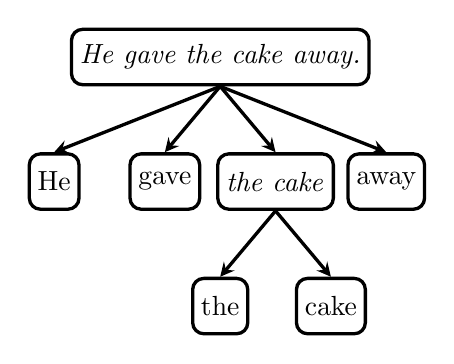
\begin{tikzpicture}[tree-style,level 1/.style={sibling distance=4em},
    level 2/.style={sibling distance=4em}, level distance=4.5em]
    \node (cla) [pattern-node] {\textit{He gave the cake away.}}
    child { node (sub)[pattern-node] {He}}		
    child { node (mv)[pattern-node] {gave}}
    child { node (com)[pattern-node] {\textit{the cake}}
        child { node (det)[pattern-node]{the}}
        child { node (nou)[pattern-node]{cake}}}
    child {node[pattern-node](adjunct)
        {away}
    };
    \end{tikzpicture}
    \caption{Representation of the Example \ref{ex:1} as constituency tree}
    \label{fig:mcg-graph-example-simple-structure}
\end{figure}

Figure \ref{fig:mcg-graph-example-simple-structure} depicts the constituency division of the clause \ref{ex:1}% which is identical to the bracket notation in Example \ref{ex:2}. 
The nodes represent grammatical constituents and the edges stand for the \textit{structure-substructure composition}. 
Next we can move on to assign constituent class and a grammatical function. Table \ref{tab:sfg-constituency-analisys} provides a constituency analysis in SFL tradition. Here the sentence is formed of a single clause which has four constituting functional parts: a Subject, a Main Verb (also known as Predicate), a Complement and an Adjunct. Each of these functional parts is filled correspondingly by a pronoun, a verb, a nominal group and an adverb as assigned in the table below.

\begin{table}[!ht]
    \centering
    \begin{tabular}{cc|c|c|c}
        \hline
        \multicolumn{1}{|c|}{\textit{He}} & \textit{gave} & \textit{the}     & \textit{cake}   & \multicolumn{1}{c|}{\textit{away.}} \\ \hline
        \multicolumn{5}{|c|}{clause}                                                                                                 \\ \hline
        \multicolumn{1}{|c|}{Subject}     & Main Verb     & \multicolumn{2}{c|}{Complement}    & \multicolumn{1}{c|}{Adjunct}        \\ \hline
        \multicolumn{1}{|c|}{pronoun}      & verb          & \multicolumn{2}{c|}{nominal group} & \multicolumn{1}{c|}{adverb}         \\ \hline
        &               & Deictic          & Thing           &                                     \\ \cline{3-4}
        &               & determiner       & noun            &                                     \\ \cline{3-4}
    \end{tabular}
    \caption{Constituency analysis with unit classes and grammatical functions}
    \label{tab:sfg-constituency-analisys}
\end{table}

Next each constituent can be assigned a set of relevant linguistic features. For example The subject ``He'' is a pronoun that has features known in traditional grammar: \textit{singular}, \textit{masculine}, and \textit{3^{rd} person}. These features are well differentiated in traditional grammar. For example \textit{singular} means \textit{non-plural}, \textit{masculine} means \textit{non-feminine} and \textit{3^{rd} person} means \textit{non-1^{st}} and \textit{non-2^{nd}}. These are closed classes meaning that there is no \textit{4^{th} person} or that there is no \textit{neutral} grammatical gender in English as other languages have. These features can be systematised (see Figure \ref{fig:traditional-pronoun}) as three systems of mutually exclusive choices that can be assigned to pronominal units. Note that the gender is enabled for 3^{rd} person singular pronouns which can be expressed as is the figure below representing a \textit{system network} (which is properly introduced in Chapter \ref{ch:sfg}).

\begin{figure}[!ht]
    \centering      
    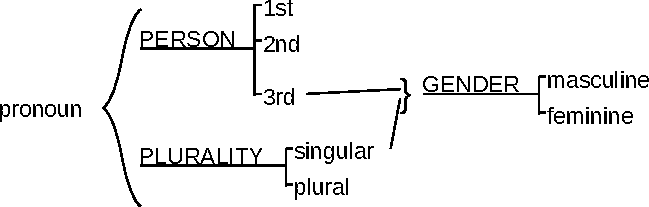
\includegraphics[width=.56\textwidth]{Figures/Example/traditional-pronoun.pdf}      
    \caption{The systematisation of three pronominal features in traditional grammar}
    \label{fig:traditional-pronoun}
\end{figure}

In SFG the pronouns are systematised in the system network of Person from \textit{Introduction to Functional Grammar} \citep[366]{Halliday2013} that is depicted in Figure \ref{fig:person-system-network}. The red rectangles from the figure represent the selections that are applicable to the Subject constituent ``He'' in example above.

\begin{figure}[!ht]
    \centering      
    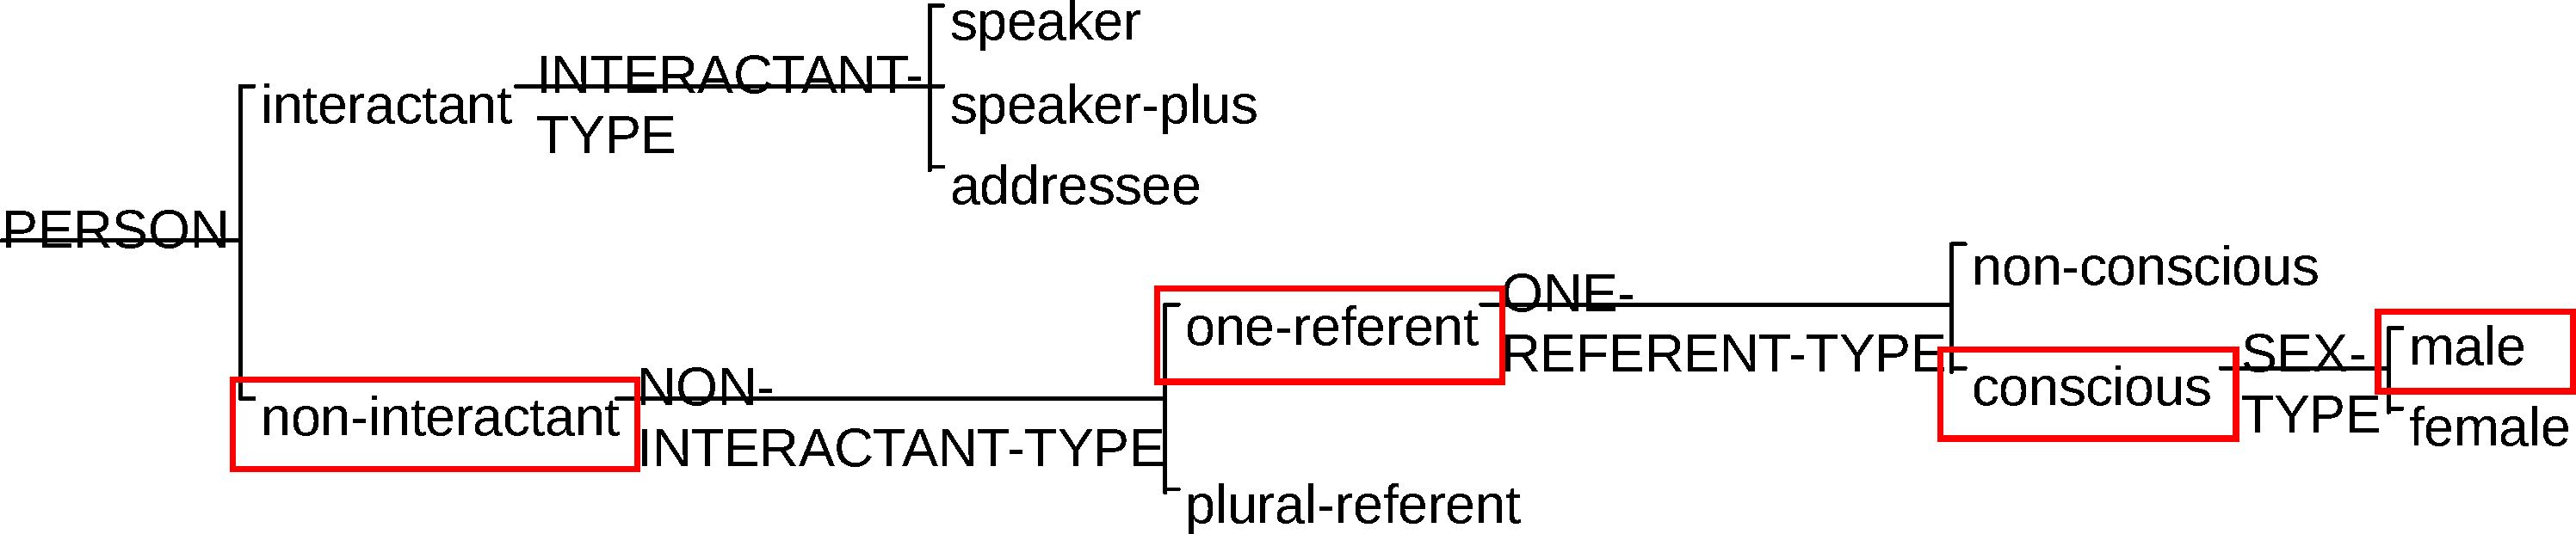
\includegraphics[width=.90\textwidth]{Figures/Example/person-selections.pdf}      
    \caption{The selections in Person system network from \citet[366]{Halliday2013} }
    \label{fig:person-system-network}
\end{figure}

Lets take now the clause constituent that is the root of the constituency tree and see how SFL features can be applied to it. If in in terms of traditional grammar the clause can be ascribed relatively few features i.e. as having \textit{passive voice}, \textit{positive polarity} and \textit{simple past tense} then in terms of SFL grammar the features are many more i.e. \textit{major, positive, active, effective, receptive, agentive, free, finite, temporal, past, non-progressive, non-perfect, declarative, indicative, mood-non-assessed, comment-non-assessed}. Figure \ref{fig:mood-selections} depicts the selections applicable to clause constituent in Example \ref{ex:1} from Mood system network that is an adaptation of Mood network proposed in \citet[162]{Halliday2013}. 

\begin{figure}[!ht]
    \centering      
    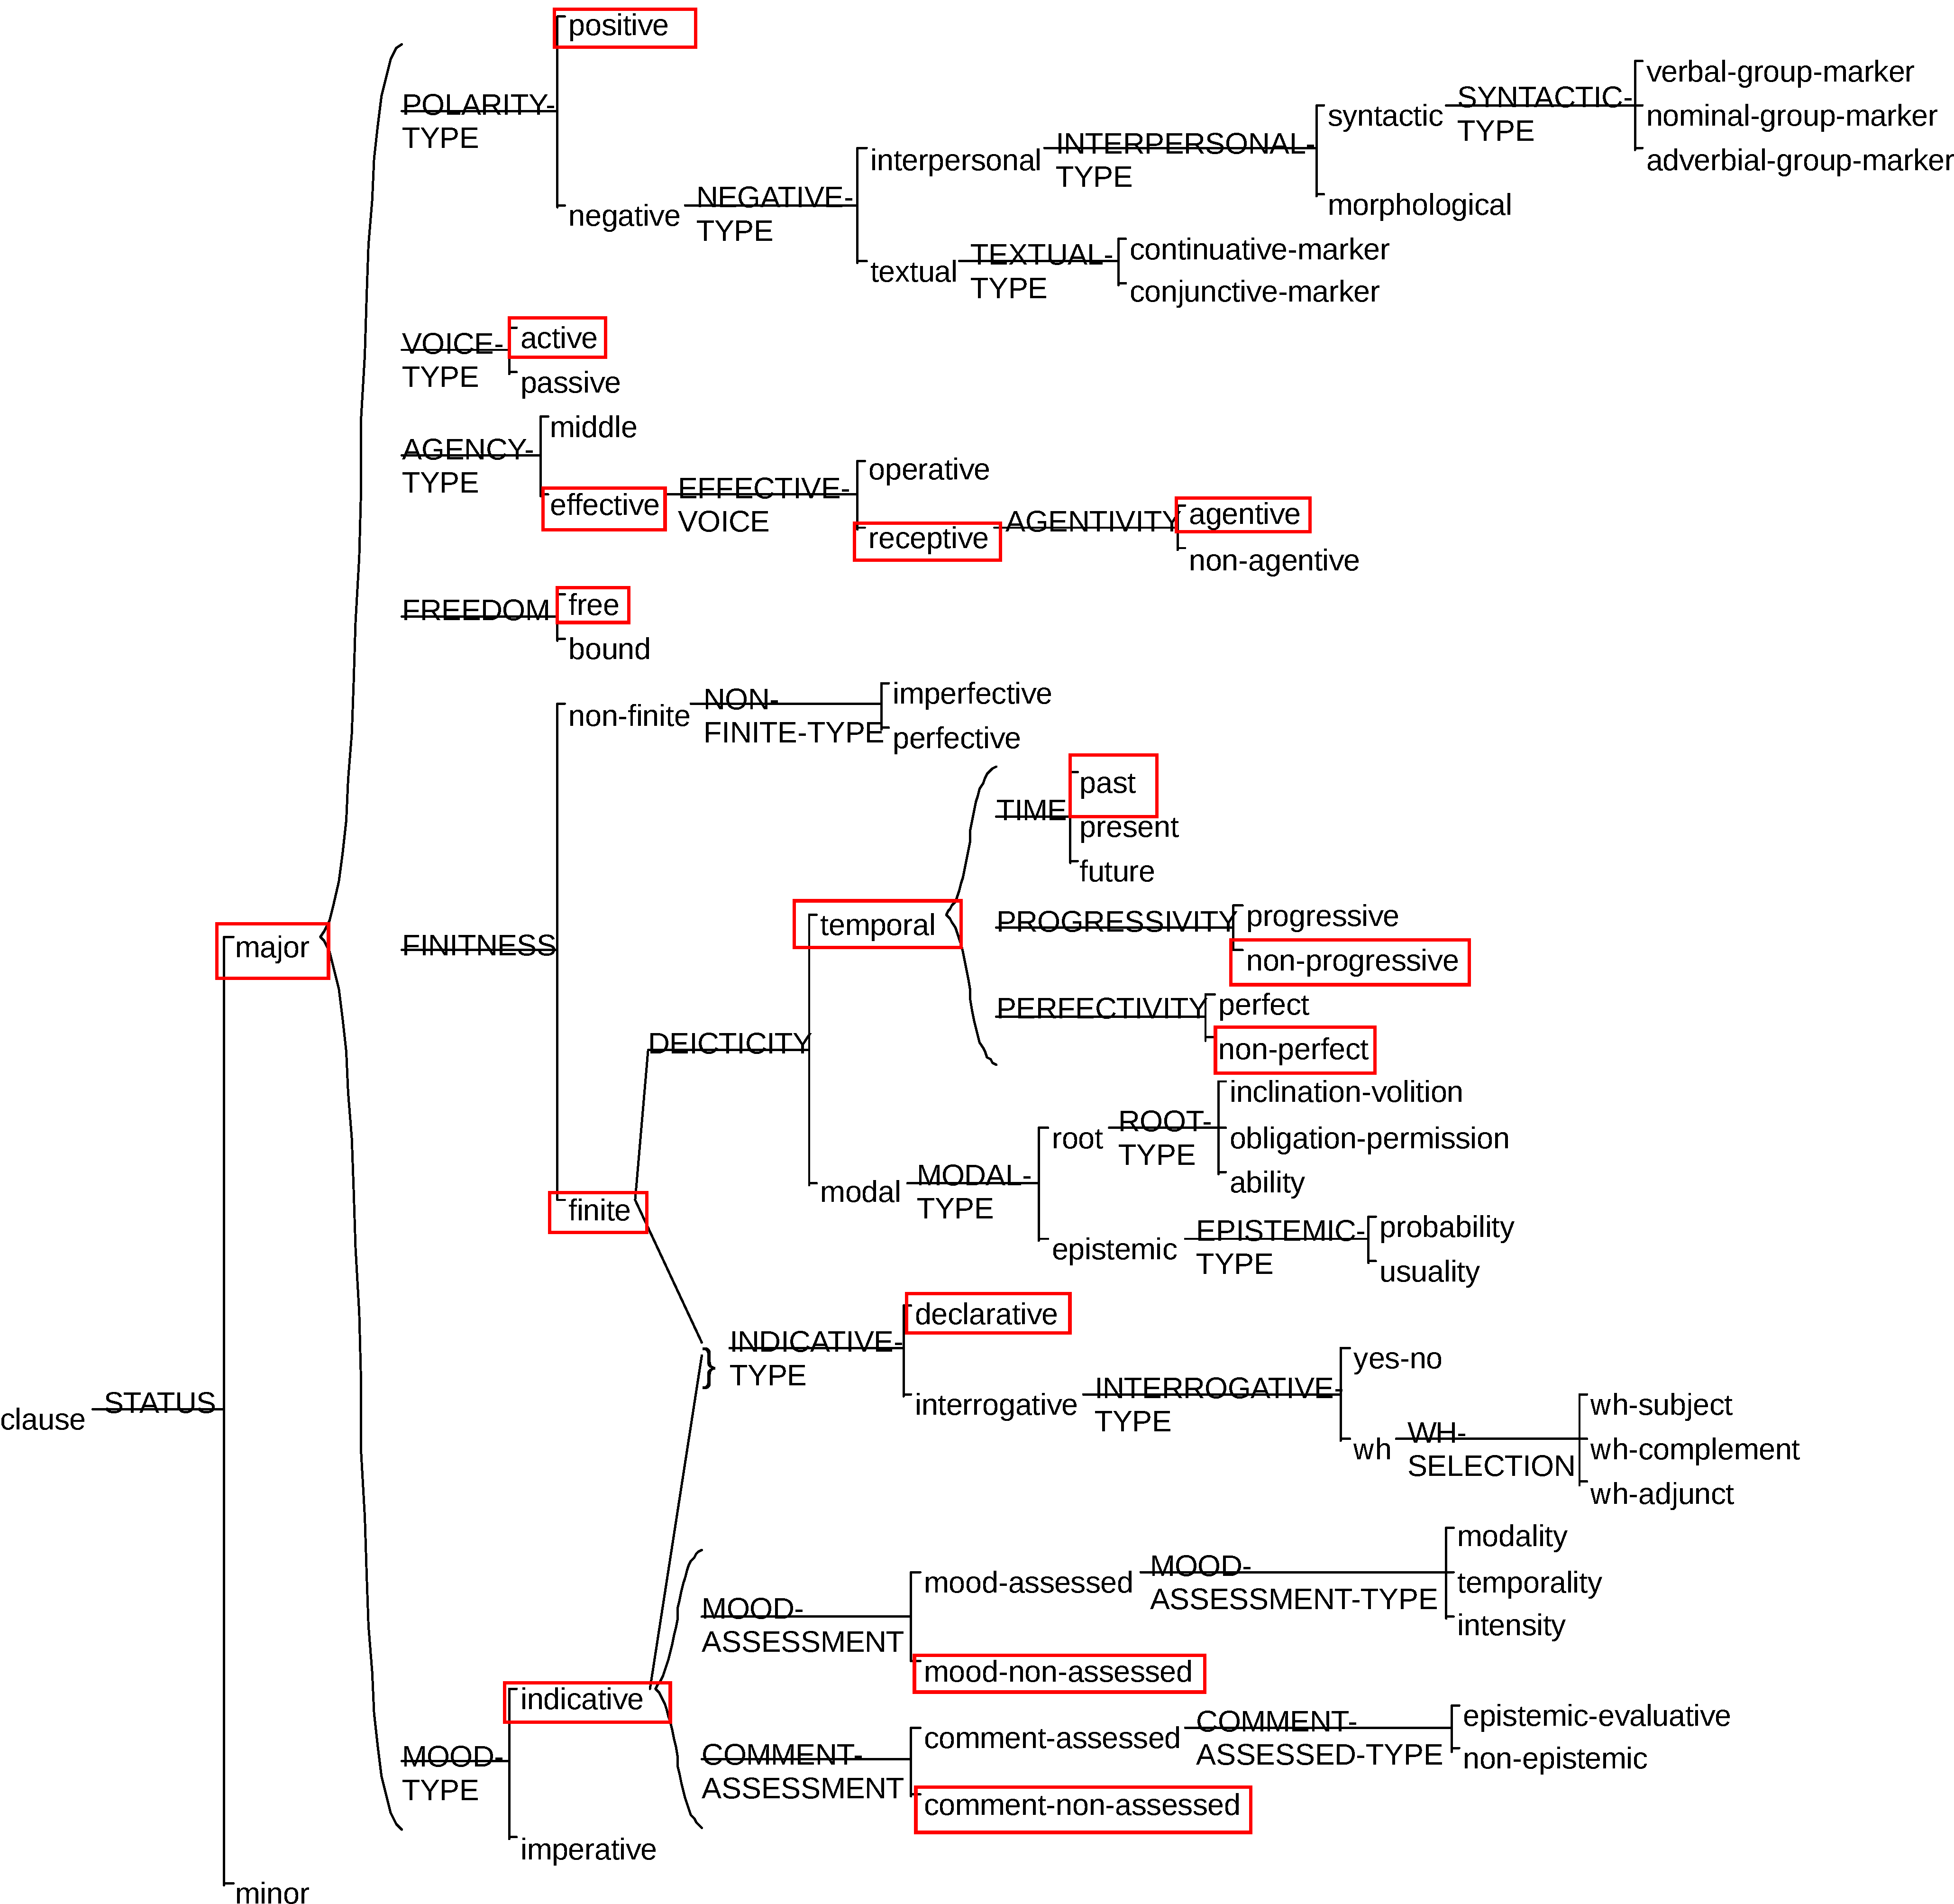
\includegraphics[width=0.91\textwidth]{Figures/Example/mood-selections.pdf}      
    \caption{The feature selections in the Mood system network for Example \ref{ex:1}}
    \label{fig:mood-selections}
\end{figure}

So far you have seen constituents assigned syntactic functions such as Subject, Complement, Adjunct etc. SFL covers a wider range of functions depending on the kind of meaning it aims at describing. For example what in other grammars is known as \textit{semantic labels}, \textit{thematic} or \textit{$\theta$ roles} SFL systematises as Transitivity system network (which will be introduced in Chapter \ref{sfg} below). Transitivity aims at providing domain independent \textit{semantic frames} called in SFL \textit{process configurations} which describe semantic actions and relationships, along with \textit{semantic roles} ascribed to their \textit{participants}. These semantic frames generally are governed by verbs and more specifically each verb meaning has a dedicated semantic frame. 

For example \ref{ex:1} corresponds to a Possessive semantic frame where ``He'' is the Agent and Carrier whereas ``the cake'' is the Possessed thing as marked in Example \ref{ex:3}. These configurations and participant roles correspond to Transitivity system network proposed in \citep{Neale2002}.

\begin{exe}
    \ex\label{ex:3} [_{Agent-Carrier} He] gave [_{Possessed} the cake] away. 
\end{exe}

There are more functions and features that can be assigned to the constituents in the Example \ref{ex:1} but I stop here. The analysis provided so far highlights that SFG grammar has a variety of functions serving to express different meanings. The traditional grammar distinguishes them as syntactic and semantic functions but, as we will see in Chapter \ref{ch:sfg} below, SFL does not make such a distinction. Another aim of the current section was to provide a glance of the feature rich grammar and I hope the example with Mood feature selection in Figure \ref{fig:mood-selections} fulfils this goal.

\begin{figure}[!ht]
    \centering
    \begin{tikzpicture}[scale=0.8, transform shape, tree-style, 
    level 1/.style={sibling distance=11em, level distance=14em},
    level 2/.style={sibling distance=10em, level distance=12em}, 
    anchor=north
    growth parent anchor = north,]
    
    \node (cla) [pattern-node, split-node, text width = 42em,]  
    {clause 
        \nodepart{two} Configuration
        \nodepart{three} major, positive, active, effective, receptive, agentive, free, finite, temporal, past, non-progressive, non-perfect, declarative, indicative, mood-non-assessed, comment-non-assessed, posessive};
    
    \node (sub) [pattern-node, split-node, below=3em of cla, xshift=-16em,] 
    {pronoun
        \nodepart{two} Subject, Participant,\\ 
        Agent \& Carrier 
        \nodepart{three} 3^{rd} person, singular,\\ 
        male, non-interactant,\\ 
        one-referent, conscious};
    
    \node (mv)[pattern-node, split-node, below=3em of cla, xshift=-5em] 
    {verb
        \nodepart{two} Main Verb, Finite, \\Process 
        \nodepart{three} possessive };
    
    \node (com)[pattern-node,split-node, below=3em of cla, xshift=6em] 
    {nominal group
        \nodepart{two} Complement, Participant, 
        \\ Affected \& Possessed
        \nodepart{three} };
    
    \node (det)[pattern-node,split-node, below=3em of com, xshift=-6em]
    {determiner
        \nodepart{two} Deictic, Modifier
        \nodepart{three} specific, demonstrative,\\ 
        determinative, non-selective};
    
    \node (nou)[pattern-node,split-node, below=3em of com, xshift=6em]
    {noun
        \nodepart{two} Thing, Head
        \nodepart{three} inanimate, singular,\\ 
        countable };
    
    \node[pattern-node,split-node, below=3em of cla, xshift=17em](adjunct)
    {adverb
        \nodepart{two} Adjunct,
        \\Circumstance,
        \\Location
        \nodepart{three} };
    
    \draw[sequence,-,edge-style] (cla.south) -- ++(0,-1em) -| (sub.north);
    \draw[sequence,-,edge-style] (cla.south) -- ++(0,-1em) -| (mv.north);
    \draw[sequence,-,edge-style] (cla.south) -- ++(0,-1em) -| (com.north);
    \draw[sequence,-,edge-style] (cla.south) -- ++(0,-1em) -| (adjunct.north);
    \draw[sequence,-,edge-style] (com.south) -- ++(0,-1em) -| (det.north);
    \draw[sequence,-,edge-style] (com.south) -- ++(0,-1em) -| (nou.north);	
    \end{tikzpicture}
    \caption{Representation of Example \ref{ex:1} as feature rich constituency graph}
    \label{fig:mcg-graph-example}
\end{figure}


Next, Figure \ref{fig:mcg-graph-example} summarises everything discussed above into a partially filled constituency tree. The constituents that were not discussed are assigned only few high level functions and features. As you can see, every node is richly decorated with syntactic and semantic features. The blue part of each node denotes grammatical class, the red part carries functions some of  which are important to establishing a valid constituency structure (that are Mood functions) and the the Transitivity functions; and the green part some grammatical features selected from system networks. In practice, the feature set is much richer than what nodes in Figure \ref{fig:mcg-graph-example} carry here the restriction aims simply to avoid an over-crowded example. 


%Generating automatically feature rich constituency structure such as the one in Figure \ref{fig:mcg-graph-example} is the general aim in the current work.

Next I describe what opportunities and limitations exist in automatically generating rich SFL analyses as until now it has not been possible to use these detailed analysis in computational contexts. This makes them unavailable for corpus work, for training data in machine learning and other end-user application scenarios provided as motivation in the Sections \ref{sec:motivation} and \ref{sec:motivation-business} above.

\section{The problem of parsing with SFGs}
\label{sec:problem}

%\todo[inline]{
%    But, until now it has not been possible to use these
%    detailed analysis in computational contexts: this makes
%    them unavailable for corpus work, for training data in
%    machine learning, etc. etc. (add as many points as occur
%    to you).
%}

%\todo[inline]{
%    There have been attempts to make this work (which you
%    will come back to and describe in Chapter X in detail), however,
%    but these have not worked. As you you say you will describe in detail
%    in Chapter X, }

%\todo[inline]{
%    there is however a strong diagnostic as to
%    just why these attempts have not been successful: i.e., the
%    lack of structural detail that SFG descriptions typically
%    provide. This is argued in general in Bateman (2008)
%    and Teich (1999) [and any other references you can find].
%}

%The problem of parsing with SFG has been well laid out in \citet{Bateman2008} as being one of computational complexity due to exponential explosion of possible combinations of features. 

SFL since it has been established has been primarily concerned with the paradigmatic axis of language. Accounts of the syntagmatic axis of language, for example syntactic structure, have been put in the background. The structure has been placed on the theoretical map and defined in terms of \textit{rank}, \textit{unit}, \textit{class} and \textit{function}, as we will see in detail in Chapter \ref{ch:sfg} but afterwards it received minimal attention as most of the focus was on the paradigmatic organisation in language (in fact this is is the feature that sets SFL apart from other approaches to study language). This has led to progress in accounting how language works at all strata but little was said about the language constituency. And this can be considered ``unsolved'' within SFL accounts leaving a ``gap in what must be one the central areas of any characterisation of language'' \citep[25]{Bateman2008}. 

%As we will see below, some accounts of constituency are provided within SFL grammars, enough even to make them applicable in computational domains such as automatic \textit{natural language generation}. But such descriptions are by far not satisfiable with respect to what would a proper syntagmatic account of language would be. 

This may be surprising as the syntagmatic dimension is implicit and present everywhere in the SFL literature. For instance all example analyses in the \textit{Introduction to Functional Grammar} \citep{Halliday2013} are predominantly syntagmatic. Moreover, Robin Fawcett for decades promotes the motto \textit{no system network without realisation statements} \citep[9]{Fawcett88-good}. \citet{Bateman2008} presents in detail why there is a severe imbalance between syntagmatic and paradigmatic axes in SFL, how it came to be this way and how it is especially damaging to the task of automatic text analysis. Next I describe the main problems and hint at how potential solutions may look like (described Section \ref{sec:solution}). 

\citet{ODonnell2005} offer a detailed description to the long history of SFL being applied in computational contexts yielding with productive outcomes on language theorising, description and processing. The transfer between SFL and computation typically involved a delay between the theoretical formulation and the computational instantiation of that formulation \citep[139]{BatemanMatthiessen88} \citep[19]{MatthiessenBateman91}. The theoretically formulated ideas contain hidden pitfalls that are revealed only upon explicit formulations required by in computation \citep[27]{Bateman2008}. 

The active exchange between the SFL theory and computation has been almost entirely oriented towards automatic \textit{natural language generation}. Such systems would use abstract semantic specifications and communicative goals to produce grammatically correct and well connected texts achieving those goals. This area has been shown to be successful in part due to decomposition of language along the paradigmatic axis using functionally motivated sets of choices between functionally motivated alternatives \citep{McDonald80}.

The computational processes driving the natural language generation relied heavily on the notion of \textit{search}. A well defined search problem is defined in terms of a precise description of the search space which then helps navigation process effectively to find solutions. The paradigmatic organization of the \textit{lexicogrammar} as system networks assumed within SFL turns out to organise the search space for possible grammatical units appropriate for communicative goals in almost ideal manner \citep[28]{Bateman2008}.

The \textit{automatic analysis} or \textit{parsing} can be seen as a reverse problem of finding appropriate analysis within a search space of possible solutions. That is identify the exact meaning, systematised in the grammar, of a given natural language sentence. As seen in Section \ref{sec:example} above, an account of the sentence meaning would have to provide both, in terms of a formal structure of the sentence revealing the constituents plus their syntactic relations to each other, and in terms of a complete set of features (detailed to the extent that grammar permits) applicable to each constituent of structure. If, in the generation process, the abstract semantic specifications are increasingly materialised through choice making by traversing the system network towards finally generated text, then, in the parsing process, the reverse is the case. The process starts from a given sentence aiming to derive/search the feature choices in the system network afferent to each of the constituents. But if the paradigmatically organised lexicogrammatical resource is effective for generation it turns out, as we will see next, to be by far unsuitable for the analysis task because of the \textit{size problem}. Halliday himself mentions this problem when he asks \textit{how big is a grammar?}.

\begin{quotation}
    Given any system network it should in principle be possible to count the number of alternatives shown to be available. In practice, it is quite difficult to calculate the number of different selection expressions that are generated by a network of any considerable complexity \citep[10]{Halliday96-grammatics}.
\end{quotation}

The issue emerges from the way connections and (cross-)classifications are organised in a system network. In addition to that, the orientation of systemic grammars towards choice means that the grammar full of disjunctions leading to the problem of search complexity. Also the abstract nature of systemic features leads to a structural richness that adds logical complexity to the task \citep{ODonnell1993}. So estimating the size of the grammar would in fact mean estimating the potential number of feature combinations. For example, a hypothetical network of 40 systems the ``size of the grammar it generates lies somewhere between 41 and 2^{40} (which is somewhere around 10^{12})'' \citep[28]{Bateman2008}. However it is not easy to predict where would the upper limit of the grammar would fall even when the configuration of relations of a particular system network is known.

For the generation task, that size, is not a problem at all as the number of choice points is actually rather small. Such a paradigmatic organisation is, in fact, an incredibly concise and efficient way to express the linguistic choices where the possible feature selections are relevant only when they are enabled by prior paradigmatic choices and it is only those alternatives that need to be considered \citep[12--13]{Halliday96-grammatics} .

In the analysis task, the paradigmatic context of choice, that helps navigation during the generation process, is no longer available. It is not known
any longer which features of a systemic network are relevant and which are not. This leads to a radical asymmetry between the two tasks. That
is: in generation, the simple traversal of the network finds only the compatible choices
because that is what the network leads to; whereas in analysis it is not evident in
advance which path to follow therefore the task is virtually to explore entire search
space in order to discover which features apply to the text. This means that any path is potentially relevant and shall be passed and checked leading to evaluation of the system network as a whole; and that there is no way to restricting the search space, as in the case of generation, to a a set of familiar paradigmatic lines \citep[29]{Bateman2008}. 

One of the grammars successfully used in generation tasks is Nigel grammar developed within Penman generation project \citep{Mann83}. It contains 767 grammatical systems defined over 1381 grammatical features which Bateman evaluates as ``a very large computational grammar by current standards, although nowadays by no means the broadest when considered in terms of raw grammatical coverage'' \citep[29]{Bateman2008}. To parse with such a grammar would means exploring an incredibly vast search space $ 3 \times 10^{18} $ to be more precise. A more detailed break down the complexity by rank or primary class as provided in Table \ref{tab:size} below.

\begin{table}[!ht]
    \centering
    \begin{tabular}{|l|r|}
        \hline
        \textit{rank or primary class} & \textit{size}                             \\ \hline
        adverbial-group                & 18                                        \\ \hline
        words                          & 253                                       \\ \hline
        quantity-group                 & 356                                       \\ \hline
        prepositional-phrase           & 744                                       \\ \hline
        adjectival-group               & 1045                                      \\ \hline
        nominal-group                  & \textgreater $ 2\times 10^{9} $  \\ \hline
        clause                         & \textgreater $ 3\times 10^{18} $ \\ \hline
    \end{tabular}
    \caption{Size of major components of the Nigel grammar expressed in terms of the number of selection expressions generated \citep[35]{Bateman2008}}
    \label{tab:size}
\end{table}

%difficulty SLR
Another difficulty in parsing with SFGs lays in the fact that, as the analysis moves away from directly observable grammatical variations towards more abstract semantic variations, the difficulty of generating an accurate account increases drastically. Transitivity system network for example consists of such semantic features and it is comparable to what is called in computational linguistics (shallow) \textit{semantic parsing} or \textit{Semantic Role Labelling} (SRL) \citep{Carreras2005}.

The main challenge of SRL (well explained in \citep[245--250]{gildea2002automatic}) remain the same since \citet{Winograd1972}: moving away from the domain specific, hand-crafted semantic specifications towards domain independent and robust set of semantic specifications. This goal was undertaken in several projects to build large broad-scope lexico-semantic databases such as WordNet \citep{Fellbaum98-wn}, FrameNet \citep{Baker1998, Johnson2000, fillmore2003background} and VerbNet \citep{schuler2005verbnet, Kipper2008}. A similar database exists for Transitivity system network as described in \citet{Fawcett2009} called Process Type Database \citep{Neale2002}. 

Such databases describe domain independent \textit{semantic frames} \citep{Fillmore1985} (know in SFL as \textit{configurations} or \textit{figures}) which describe semantic actions and relationships, along with \textit{semantic roles} ascribed to their \textit{participants}. The semantic frames generally are governed by verbs and more specifically each verb meaning has a dedicated semantic frame. For instance the perception frame contains \textit{Perceiver} and \textit{Phenomenon} roles as can be seen in Example \ref{ex:glance1}. 

\begin{exe}
    \ex\label{ex:glance1} [_{Agent-Perceiver} Jaqueline] glanced [_{Phenomenon} at her new watch].
\end{exe}

The tendency is to identify frames that are generic enough to cover classes of verb meanings (for example Action, Cognition, Perception, Possession frames) and the same applies to participant roles where the tendency is to reuse roles across semantic frames (for example agent role from Action frame is reused in Perception or Possession frames, or Phenomenon is reused in Cognition and Perception frames).

%example of covert constituents
Besides the challenge of pinning them down in text, the problem with semantic features goes one step further. Sometimes the semantic roles correspond to constituents that are displaced or not even realised in the text. This increases the challenge of identifying and assigning them correctly. Consider Example \ref{ex:glance2}. It is a sentence that has three non-auxiliary verbs: seem, worry and arrive. According to Cardiff grammar, which will be introduced in Chapter \ref{ch:sfg}, this corresponds to three clauses \textit{embedded} into each other as represented in Table \ref{tab:glance-analsys}.

\begin{exe}
    \ex\label{ex:glance2} She seemed to worry about missing the river boat.
%    \ex\label{ex:glance3} She seemed [to worry [about missing the river boat]].
\end{exe}

\begin{table}[!ht]
    \centering
    \resizebox{\columnwidth}{!}{%
    \begin{tabular}{cccc|c|c|c|c|c|}
        \hline
        \multicolumn{1}{|c|}{\textit{She}} & \multicolumn{1}{c|}{\textit{seemed}} & \multicolumn{1}{c|}{\textit{to}}        & \textit{worry} & \textit{about} & \textit{missing} & \textit{the} & \textit{river} & \textit{boat.} \\ \hline
        \multicolumn{9}{|c|}{clause}                                                                                                                                                                                              \\ \hline
        \multicolumn{1}{|c|}{Subject}      & \multicolumn{1}{c|}{Main Verb}       & \multicolumn{7}{c|}{Complement}                                                                                                               \\ \hline
        & \multicolumn{1}{c|}{}                & \multicolumn{7}{c|}{clause}                                                                                                                   \\ \cline{3-9} 
        & \multicolumn{1}{c|}{}                & \multicolumn{1}{c|}{Infinitive Element} & Main Verb      & \multicolumn{5}{c|}{Complement}                                                    \\ \cline{3-9} 
        &                                      &                                         &                & \multicolumn{5}{c|}{clause}                                                        \\ \cline{5-9} 
        &                                      &                                         &                & Binder         & Main Verb        & \multicolumn{3}{c|}{Complement}                \\ \cline{5-9} 
    \end{tabular}%
    }
    \caption{SF constituency analysis in Cardiff grammar style}
    \label{tab:glance-analsys}
\end{table}

The participant role configurations (or the semantic frames) these verbs bring about are provided in the Table \ref{tab:semantic-role-distro}. For the sake of this example lets say that the first role corresponds to the Subject constituent and the second to the Complement constituent. This way the verb meaning seem_{1} corresponds to an Attributive configuration that distributes Carrier and Attribute roles to the Subject ``She'' and the Complement ``to worry about missing the river boat''. In the case of worry about_1 and miss_1 the first roles provided by Cardiff grammar are \textit{compound} (i.e. composed of two simple ones) while the second ones are simple. So, in the example above, the verb meaning worry about_1 distributes the Phenomenon to the Complement ``about missing the river boat'' and the Agent \& Cognizant role to an empty Subject that is said to be \textit{non-realised}, \textit{covert} or \textit{null element}. A similar situation is for miss_1 that assigns an Affected \& Carrier role to the empty Subject and the Possessed role to the Complement ``the river boat''. 

\begin{table}[!ht]
    \centering
    \begin{tabular}{|l|l|l|}
        \hline
        \textit{verb meaning} & \textit{semantic configuration} & \textit{participant role mandatory distribution}  \\ \hline
        seem_{1}           & Attributive                     & Carrier + Attribute                     \\ \hline
        worry about_{1}   & Two Role Cognition              & Agent \& Cognizant + Phenomenon         \\ \hline
        miss_{1}           & Possessive                      & Affected \& Carrier + Possessed (thing) \\ \hline
    \end{tabular}
    \caption{Semantic role configurations according to \citet{Neale2002,Fawcett2009}}
    \label{tab:semantic-role-distro}
\end{table}

Those unrealised Subjects in the embedded clauses are recoverable from the immediate syntactic context (no need for discourse) and correspond, in this case, to the Subject in the higher clause. This is easy to see in Examples \ref{ex:glance3} and \ref{ex:glance4} therefore we can just mark the places of the null Subjects in the embedded clause in order to be able to assign the semantic labels (otherwise the frame cannot be assigned to the constituents). Notice that I have provided also an index \textit{i} to highlight that the null elements correspond to the higher clause Subject ``She''. 

\begin{exe}
    \ex\label{ex:glance3} \textit{She} worried about missing the river boat.
    \ex\label{ex:glance4} \textit{She} missed the river boat.
    \ex\label{ex:glance5} She_i seemed [\textit{null-Subject}_i to worry [about \textit{null-Subject}_i missing the river boat]].
\end{exe}

Now that the places of covert constituents are explicitly marked and the recoverable constituent coindexed we can see the distribution of semantic roles realised for this sentence in the Table \ref{tab:glance-analsys-semantic} below. 

\begin{table}[!ht]
    \centering
    \resizebox{\textwidth}{!}{%
        \begin{tabular}{cccccc|c|c|c|c|c|}
            \hline
            \multicolumn{1}{|c|}{\textit{She_i}}   & \multicolumn{1}{c|}{\textit{seemed}} & \multicolumn{1}{c|}{\textit{null_i}}   & \multicolumn{1}{c|}{\textit{to}} & \multicolumn{1}{c|}{\textit{worry}} & \textit{about} & \textit{null_i}    & \textit{missing} & \textit{the} & \textit{river} & \textit{boat.} \\ \hline
            \multicolumn{11}{|c|}{Attributive configuration}                                                                                                                                                                                                                         \\ \hline
            \multicolumn{1}{|c|}{Agent} & \multicolumn{1}{c|}{}       & \multicolumn{9}{c|}{Attribute}                                                                                                                                                                               \\ \cline{1-1} \cline{3-11} 
            & \multicolumn{1}{c|}{}       & \multicolumn{9}{c|}{Two Role Cognition configuration}                                                                                                                                                        \\ \cline{3-11} 
            & \multicolumn{1}{c|}{}       & \multicolumn{1}{c|}{Agent \& Cognizant} &                         & \multicolumn{1}{c|}{}               & \multicolumn{6}{c|}{Phenomenon}                                                                       \\ \cline{3-3} \cline{6-11} 
            &                             &                                      &                         & \multicolumn{1}{c|}{}               & \multicolumn{6}{c|}{Possessive configuration}                                                         \\ \cline{6-11} 
            &                             &                                      &                         &                                     &                & Affected \& Carrier &                  & \multicolumn{3}{c|}{Possessed}                 \\ \cline{7-7} \cline{9-11} 
        \end{tabular}%
    }
    \caption{Transitivity analysis in Cardiff grammar style \citep{Neale2002,Fawcett2009}}
    \label{tab:glance-analsys-semantic}
\end{table}

In language there are many cases where constituents are empty but recoverable from the immediate vicinity relying in most cases on syntactic means and in a few cases additional lexical-semantic resources are required. The mechanisms of detecting and resolving the empty constituents are captured in the Government and Binding Theory (GBT) developed in \citep{Chomsky81, Chomsky1982, Chomsky1986} and based on the phrase structure grammar. GBT explains how some constituents can \textit{move} from one place to another, where are the places of \textit{non-overt constituents} and what constituents do they refer to i.e. what are their \textit{antecedents}. Such accounts of empty elements are missing from any SFG grammar yet they are useful in determining the correct distribution of participant roles to the clause constituents. Translating the mechanisms from GBT into SFG could contribute to decreasing the complexity of the parsing problem mentioned above.

% concluding problem

To conclude, I have drown attention to a few issues related to parsing with SFG. First, the parsing task cannot be treated as a reversible generation task because the methods that have been shown to work for generation are not usable for parsing as such due to a high computational complexity. Second, the parsing task, regardless of the grammar, should first and foremost account for the sentence structure on the syntagmatic axis and only afterwards for the (semantic) features selected on the paradigmatic axis. Such syntagmatic account in SFL is insufficient for the parsing task. Third, syntagmatic account alone does not provide enough clues for assignment of semantic features and require a lexical-semantic account within the grammar or as external semantic databases. Moreover it can be aided by identification of places where covert constituents are said to exist. Identifying such the null elements is not the only method of assigning semantic features and some approaches do without them but having access to such information is considered valuable in the present thesis.

Considering the problems above how could the vast search space of grammars such as Nigel be restricted to a reasonable size and how can be compensated the lack of proper syntagmatic description in SFGs? The first part of the question has already been addressed in \citet{ODonnell1993} but the lack for an answer to the second part and probably for other hidden reasons the results are not usable in real world applications. There have been, in fact, multiple attempts such as \citet{Kasper1988}, \citet{Kay1985}, \citet{ODonoghue1991a}, \citet{ODonnell1993} and \citet{Day2007}, to mention just a few, none of which managed to parse broad coverage English with full SFG without aid of some sort. Each had to accept limitations either in grammar or language size and eventually used simpler syntactic trees as a starting point of the parsing process. A detailed account of the current state of the art in parsing with SFGs is provided in Chapter \ref{ch:sota}. 

Some linguistic frameworks, other than SFL, have been shown to work well in computational contexts solving problems similar to the ones identified above. Instead of attempting to find novel solutions within the current framework an alternative approach, I argue in the next section, would be to establish cross-theoretical and inter-grammatical links to enable integration of the ready solutions.

\section{On theoretical compatibility and reuse}
\label{sec:reuse}
% reuse motivation, context to parsing 
In the past decades many significant progresses have been made in natural language parsing framed in one or another linguistic theory each adopting a distinct perspective and set of assumptions about language. The theoretical layout and the available resources influence directly what is implemented into the parser and each implementation approach encounters challenges that may or may not be common to other approaches in the same or other theories. 

Parsers implementing one theoretical framework may face common or different challenges to those implementing other frameworks. The converse can be said of the solutions. When a solution is achieved using one framework it is potentially reusable in other ones. The successes and achievements in any school of thought can be regarded as valuable cross theoretical results to the degree links and correspondences can be established. Therefore reusing components that have been shown to work and yield ``good enough results'' is a strong pragmatic motivation in the present work.

%
This thesis employs three linguistic frameworks namely the \textit{Systemic Functional Linguistics}, \textit{Dependency Grammar} and \textit{Governance \& Binding Theory}. SFL has already been motivated as target analysis framework in Section \ref{sec:framework} which is in detail introduced in Chapter \ref{ch:sfg}. The other two frameworks are employed because some of the accomplishments in those domains I attempt at reusing in this thesis as motivated below. 

%The compatibility
%It demonstrates how selected grammatical frameworks namely \textit{Systemic Functional Grammar}, \textit{Dependency Grammar} and \textit{Governance \& Binding Theory} relate to each other and to which degree they are compatible to undergo a conversion process and to show that simple patterns carrying grammatical information can be used to enrich syntactically and semantically the parse structures. And here is a brief motivation for selecting these frameworks.   

%
In the last years \textit{Dependency Grammar} \citep{Tesniere2015} became quite popular in natural language processing world favoured in many projects and systems. The grammatical lightness and the  modern algorithms implemented into dependency parsers such as Stanford Dependency Parser \citep{Marneffe2006}, MaltParser \citep{Nivre2006}, MSTParser \citep{McDonald2006} and Enju \citep{Miyao2005} are increasingly efficient and highly accurate. Among the variety of dependency parsing algorithms, a special contribution bring the \textit{machine learning} methods such as those described in \citet{mcdonald2005online, mcdonald2006online, carreras2007experiments, zhang2011transition, pei2015effective} to name just a few. 

As the dependency parse structures provide information about functional dependencies between words and grants direct access to the predicate-argument relations and can be used off the shelf for real world applications. 
This information alone makes the dependency grammar a suitable candidate to supplement the syntagmatic account missing in SFGs and provide some functional hooks for reducing complexity in parsing with SFGs. One of the goals in this work is to investigate to which degree the dependency grammar is structurally and functionally compatible with SFGs to undergo a cross theoretic transformation. This hypothesis is investigated at the theoretical level in Chapter \ref{ch:dependecy-grammar} and then indirectly evaluated empirically in Chapter \ref{ch:evaluation} based on Stanford Dependencies parser version 3.5 \citep{Marneffe2008a,Marneffe2008, Marneffe2014}. 

The problem of accounting for the \textit{null elements}, mentioned above, is not addressed neither in SFL nor in Dependency Grammar. It is, however, in detail addressed in the Government and Binding Theory (GBT) \citep{Chomsky81,Haegeman1991} which is one of Chomsky's Transformational Grammars \citep{Chomsky1957}. One other goal in this thesis is to investigate to which degree GBT accounts of null elements can be reused as DG or SFG structures to undergo a cross-theoretic transformation enabling those accounts in DG or SFG contexts. In Chapter \ref{ch:gbt} I introduce GBT and investigate this hypothesis providing some of the cross-theoretic and inter-grammatical links to Dependency and SFL grammars that as we will see in Chapter \ref{ch:semantic-parsing} benefits the Transitivity analysis.

%Chapter \ref{ch:dependecy-grappamr} and \ref{ch:gbt} besides introducing the Dependency grammar and correspondingly Government and Binding Theory show how these frameworks relate to each other and to which degree they are compatible to undergo a conversion process for the purpose of reuse.

\section{Thesis Goals and Proposed Solution}
\label{sec:solution}

This thesis aims at a reliable modular method for parsing unrestricted English text into a feature rich constituency structure using Systemic Functional Grammar (SFG).

As will be described in Chapter \ref{sec:sota}, some parsing approaches use a syntactic backbone which is then flashed out with an SFG description. Others use a reduced set or a single layer of SFG representation; and the third group use an annotated corpus as the source of a probabilistic grammar. Regardless of approach, each limits the SFG in one way or another, balancing the depth of description with language coverage: that is either \textit{deep description but a restricted language} or \textit{shallow description but broad language coverage} is attempted. The current thesis tilts towards the latter: while keeping the language coverage as broad as possible the aim is to provide, in the parse result, as many systemic features as possible.

The process developed in this thesis can be viewed as a pipeline architecture (see Section \ref{sec:architecture}) comprising of two major phases: the \textit{structure creation} and the \textit{structure enrichment}. The structure creation phase aims to account for the syntagmatic dimension of language. 

The structure enrichment phase aims at discovering and assigning systemic features (accounting for the paradigmatic dimension of language) afferent to each of the nodes constituting the structure. In this phase, two kinds of feature enrichments can be distinguished by the kinds of clues used for feature identification. The first kind of clues are syntagmatic (constituency tree, unit class, unit function, linear order, position) and can be detected using, what I call, the \textit{structural patterns} while the second kind of clues are lexical-semantic requires lexical-semantic and potentially more kinds of resources in addition to the structural patterns.

\subsection{Towards the syntagmatic account}
\label{sec:syntagmatic-account}
%solution to syntagmatic deficit
The problem in using SFGs for parsing, as we have seen in Section \ref{sec:problem} above, manifests when the grammar is instantiated computationally with a primary focus on paradigmatic organisation (prevalent in SFL) at the cost of syntagmatics which leads to the first difficulty that needs to be addressed: discovering from a sequence of words what possible groups are combinable into grammatical groups, phrases or clauses. This is a task of bridging a sequence of words as input and the grammatical description of how they can combine to form a (syntactic) constituency tree structure (known in SFL as \textit{syntagmatic organizations} which will be addressed in Section \ref{sec:structure-sydney}). 

This challenge can be addressed by filling the gap of the syntagmatic account within the SFL grammar directly. It involves, first, providing information about which grammatical functions operate at each rank, second, which grammatical functions can be filled by which classes of units and, third, providing relative and absolute description of the element order for each unit class. This information in the grammar can guide the process of building the constituency structure. 

Alternatively the problem of structure construction can be outsourced as parsing with other grammars. This is done in the works of Kasper \citet{Kasper1988} and \citet{Honnibal2004a, Honnibal2007} and is knows in SFL literature as \textit{parsing with a syntactic backbone}. In this case, the problem changes into creating a transformation mechanism to obtain the SFL constituency structure rather than build it from scratch. 

%Starting the SFG parsing process from a syntactic tree produced with other grammars reduces the computational complexity and the search space discussed in Section \ref{sec:problem} above. 

This thesis addresses the problem of building the constituency structure by the latter approach: parsing the text with Stanford Dependencies parser version 3.5 \citep{Marneffe2008a,Marneffe2008, Marneffe2014} and then transforming the parse result into SFG constituency tree. The transformation mechanisms from one grammar into the other one requires also a theoretical discussion in terms of what is being transformed. Such account of linguistic primitives or configurations of primitives in the source grammar corresponds to SFG primitives is provided in Chapter \ref{ch:dependecy-grammar}. 

The SFG constituency structures is generated through a process that involves: traversing the source (dependency) parse tree and, at each traversal step, executing a constructive operation on a parallel tree following a predefined rule set of operations and mapping relations. The detailed description of the structure generation process is provided in the Chapter \ref{ch:parsing-algorithm}. 

%todo provide example

\subsection{Towards the paradigmatic account}
\label{sec:paradigmatic-account}
Once the constituency structure is in place it can inform the following feature derivation process. The configurations of units of specific classes and carrying grammatical functions can operate as ``hooks'' on system network to guide the traversal in the same way the paradigmatic context available in the generation process. Such configurations resemble the SFG \textit{realization rules} which, in the generation process, instantiate the (abstract) features into text. 

\begin{figure}[!ht]
    \centering      
    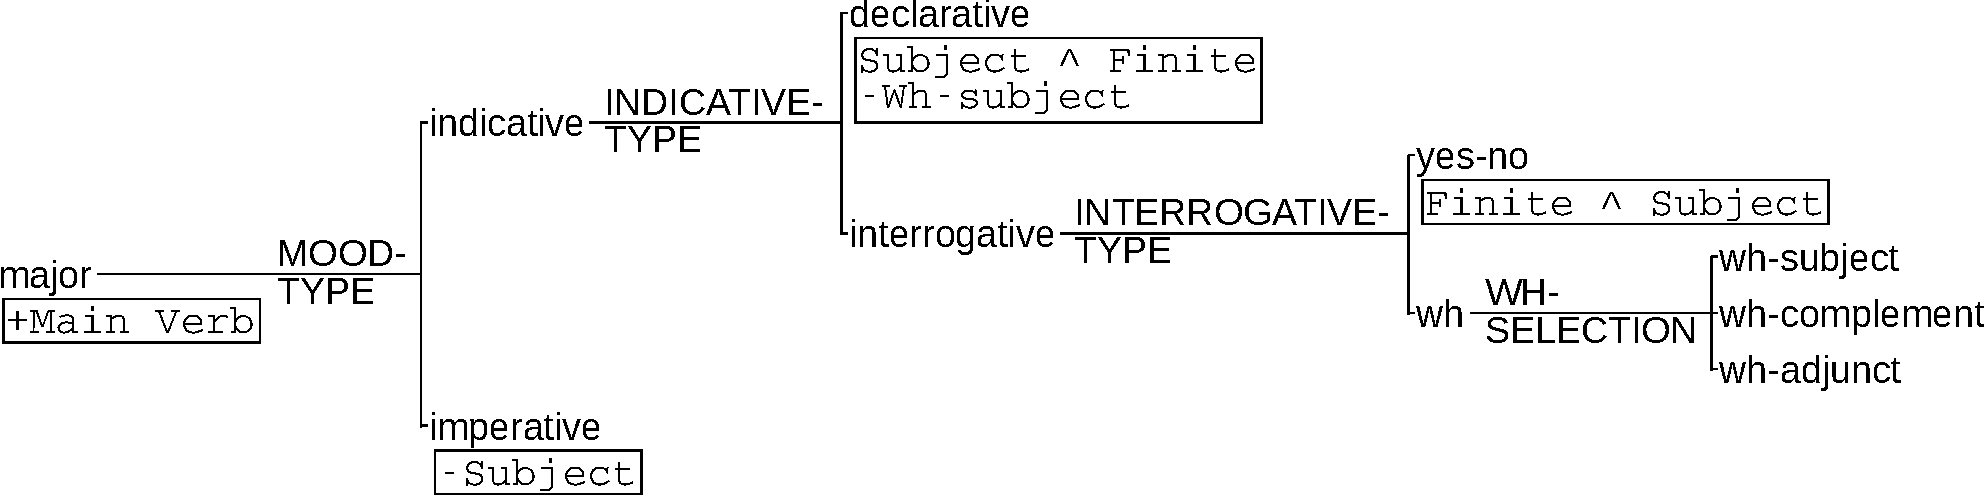
\includegraphics[width=0.91\textwidth]{Figures/Example/just-mood.pdf}      
    \caption{A fragment of mood system from \citet[366]{Halliday2013}}
    \label{fig:just-mood}
\end{figure}

The system network fragment in Figure \ref{fig:just-mood} contains the realisation rules positioned in rectangles below a few features. These realisation rules indicate what shall be reflected in the structure when a feature is selected (discussed already in Section \ref{sec:problem}). The converse is also true: if structure contains a certain pattern then it is a (potential) manifestation of a given feature.

For example the structure of a \textit{major} clause needs to have a predicate or Main Verb element realised. In the parsing process, testing whether there is a unit functioning as Main Verb below in the clause node suffices to assign the \textit{major} feature to that clause. Next, if the clause has no unit functioning as Subject then it shall be assigned \textit{imperative} feature otherwise the \textit{indicative} one. Further the INDICATIVE-TYPE system is enabled. Here the test is whether a Subject node is positioned in front of the Finite node and whether the Subject contain the preposition ``who''. This sort of queries on the structure can be formulated as \textit{structure patterns} (see Section \ref{sec:pattern-graphs}) and associated to features in the system network in the same manner the realisation rules are. 

The pattern recognition plays an essential role in current parsing method for fleshing out the constituent backbone with systemic selections. In the parsing process the structural patterns are tested whether they \textit{match} (see Section \ref{sec:pattern-graph-matching}) anywhere in the constituency structure and if so then the matched nodes are enriched with the features proved in the pattern (described in Section \ref{sec:pattern-based-operations}). 

The structural patterns in this work are expressed as \textit{graph patterns} (described in Section \ref{sec:pattern-graphs}). Note that I employ graph and not tree patterns because the tree patterns are too restrictive for the purpose of the current work. While most of the time they are hierarchically structured as a tree there are few patterns that involve sibling connections or nodes with more than one parent. In both cases the tree structure is broken. The graph approach allows a wide range of structures which also includes the trees. 

The enrichment stage of the parsing process comprises of a series of graph pattern matching operations that in case of success leads to the enrichment of the constituency structure with the features given in the graph pattern. This mechanism is described in detail in the Section \ref{sec:enrichment-stage}. 

In this work most of the graph patterns have been manually created. Because this is laborious exercise only a few system networks have been covered in the implementation of the parser. Nonetheless they suffice for deriving some conclusions regarding the parsing approach. The future work may investigate how can graph patterns be generated automatically from the realisation rules of large grammars such as Nigel grammar. 

The two main system networks targeted in this are MOOD and TRANSITIVITY (both briefly described in Chapter \ref{ch:sfg}). The MOOD network is composed of features which can be identified through graph patterns involving only the unit classes and functions provided in the constituency structure (described in Chapter \ref{ch:parsing-algorithm}). The TRANSITIVITY network requires a lexical-semantic database in order to derive graph patterns. This work employs the Process Type Database (PTDB) \citep{Neale2002} to aid enrichment with TRANSITIVITY features described in Chapter \ref{ch:semantic-parsing}.  



%Moreover if the syntagmatic account is available then they can serve as paradigmatic context (similar to the one available during generation task) for traversing the system network and extend to the full set of systemic features. This sort of description can restrict the search space to applicable network parts and provide to an extent traversal context during analysis task.


%...

%solution to feature enrichment. Transitivity


%The second stage of constituent enrichment by network traversal can be further aided by checking an arbitrary set of patterns for preselecting even more features recoverable via lexico-syntactic patterns. 


%\todo[inline]{I Reuse the structural account from other theories}
%\todo[inline]{
%    Your proposed solution to this problem, and the goal of the thesis,
%    is therefore to add some more structural information to a
%    complete augmented SFG account by drawing on frameworks which
%    have demonstrated coverage of structural detail and which
%    also have supported computational instantiation. This will
%    be shown and evaluated in the thesis.}
%
%\todo[inline]{
%    Reuse structural accounts from other theories that have shown to work well computationally.
%Could use famous Chomskyan approach but will use it latter for a more specific problem, that of finding covert constituents (give example of null subject in embedded clause). Instead I turn to Dependency Grammar that increasingly gained popularity in the last 15 years. It has been shown to be computationally fast and it is compatible in many ways with SFG which I will show latter how (mapping DG to SFG). }
%
%\todo[inline]{how: (1) by aligning the primitives and drawing cross-theoretical bridges (see section X), (2) then by mapping grammars (see section Y), (3) implemented using graph transformations (see section Z)}
%
%\todo[inline]{II Enrich the constituency structure with features (since the original goal is to have rich language analysis), that in traditional sense are spanning from purely syntactic (such as tense, voice, case, gender, number etc.) or more semantic or even pragmatic (such as semantic role labels, speech acts, sentiment and appraisal and others) }
%
%\todo[inline]{how: (1) by mapping structure to features (SFL Mood) (see section X), (2) by mapping lexical-semantic resources to fragments of syntactic structure and lexis (lexis contextualised by syntactic structure) (SFL Transitivity) (see section Y), (3) implemented by graph pattern matching (see section Z)}
%
%\todo[inline]{
%    So, the thesis goal and outline will be to (and you list them
%    explicitly like this too):\newline
%    - characterise SFL in its two major variants\newline
%    - characterise the previous attempts to parse with SFL and their problems\newline
%    - set out two further linguistic frameworks which (a) have\newline
%    strong accounts of structural relationships, (b) have shown
%    themselves supportive of computational instantiation, and (c) can
%    be shown to exhibit suggestive theoretical/descriptive
%    links with SFG: in particular, DG and GB.
%    
%    Chapter X does this for DG
%    Chapter Y does this for GB.}

\subsection{The Implementation Architecture}
\label{sec:architecture}
The current thesis is accompanied by a software implementation called Parsimonious Vole parser. It is written using Python programming language and is available as open source distribution (\url{https://bitbucket.org/lps/parsimonious-vole}).

The parser follows a pipeline architecture depicted in Figure \ref{fig:pipeline-overview} where, starting from an input text, a rich systemic functional constituency structure is progressively built. This section provides an overview to the construction process. 

The figure provides three types of boxes. The rounded rectangles represent the parsing steps. 
%The trapezoid bodes represent data of various kinds. 
The parsing steps linearly flow from one to the next via green trapezoid boxes on the left-hand side, which represent input-output data data intermediating the processes. On the right-hand side are positioned double edged orange trapezoids representing fixed resources used as additional input for some steps. For example, the \textit{constituency graph creation} step takes a normalised dependency graph for input and produces a constituency graph as output.

On the right-hand side a series of green vertical arrows are provided naming phases in parsing process (spanning one ore more process steps) where the first thee  i.e. Bootstrapping, Pre-processing and Graph Building accomplish construction of the constituency backbone (corresponding to the syntagmatic account described in Section \ref{sec:syntagmatic-account} above) and the last phase \textit{Graph Enrichment} (spanning three process steps) flashes out the backbone with features (described in Section \ref{sec:paradigmatic-account}). 

\begin{figure}[!ht]
    \begin{tikzpicture}[node distance=1.2em, scale=0.85, transform shape]
    % aLVL 0
    \node[](data) {}; % invisible node
    \node[right=12em of data](process) {}; % invisible node
    \node[right=12em of process](resource) {}; % invisible node 
    \node[right=9.5em of resource](flow) {}; % invisible node 
    
    % aLVL 1
    \node[data,anchor=center, below=-2em of data] (text) {Input Text};
    \node[task,anchor=center, below=-2em of process] (dep-parse) { Dependecy Parsing};
    \draw[sequence,->] (text) -- (dep-parse);
    
    % aLVL 2
    \node[data,anchor=center, below=6.5em of data] (dep-graph) {Dependecy Graph};
    \node[task,anchor=center, below=6em of process] (correction) {Error Correction \& \\ Graph Normalization};
    \draw[sequence,->] (dep-graph) -- (correction);
    \draw[sequence,->] (dep-parse.south) -- ++(0,-1.5em)  -| (dep-graph.north);
    
    % resources
    \node[persistent-data,anchor=center, below=4em of resource] (error-graph) {Common Error \\ Graph Patterns};
    \node[persistent-data,anchor=center, below=8em of resource] (norm-graph) {Normalization \\ Graph Patterns};
    
    \draw[sequence,->] (error-graph.west) -- ++(-1.5em,0)  |- (correction.east);
    \draw[sequence,->] (norm-graph.west) -- ++(-1.5em,0)  |- (correction.east);
    
    % aLVL 3
    \node[data,anchor=center, below=14em of data] (norm-dep-graph) {Normalised \\ Dependency Graph };
    \node[task,anchor=center, below=14em of process] (const-cr) {Constituency Graph \\ Creation};
    \draw[sequence,->] (norm-dep-graph) -- (const-cr);
    \draw[sequence,->] (correction.south) -- ++(0,-1.5em)  -| (norm-dep-graph.north);
    
    % resources
    \node[persistent-data,anchor=center, below=14.43em of resource] (rule-table) {Rule Table}; % 12.425
    \draw[sequence,->] (rule-table.west) --  (const-cr.east);
    
    % aLVL 4
    \node[data,anchor=center, below=24em of data] (const-gr) {Constituency Graph };
    \node[task,anchor=center, below=23.5em of process] (const-gr-enr) {Constituency Graph \\ Enrichment};
    \draw[sequence,->] (const-gr) -- (const-gr-enr);
    \draw[sequence,->] (const-cr.south) -- ++(0,-1.5em)  -| (const-gr.north);
    
    %resources
    \node[persistent-data,anchor=center, below=21em of resource] (sys-net) {System Network};
    \node[persistent-data,anchor=center, below=23.5em of resource] (feat-dict) {Feature-rich \\ Dictionaries};
    \node[persistent-data,anchor=center, below=27em of resource] (sys-feat-gm) {Systemic Feature \\ Graph Patterns};
    \draw[sequence,->] (feat-dict.west) --  (const-gr-enr.east);
    \draw[sequence,->] (sys-net.west) -- ++(-.79em,0)  |- (const-gr-enr.east);
    \draw[sequence,->] (sys-feat-gm.west) -- ++(-1.5em,0)  |- (const-gr-enr.east);
    
    % aLVL 5
    \node[data,anchor=center, below=31.5em of data] (enriched-gr) {Feature Enriched \\ Constituency Graph };
    \node[task,anchor=center, below=31.5em of process] (null-cr) {Null Element \\ Creation};
    \draw[sequence,->] (enriched-gr) -- (null-cr);
    \draw[sequence,->] (const-gr-enr.south) -- ++(0,-1.5em)  -| (enriched-gr.north);
    
    %resources
    \node[persistent-data,anchor=center, below=31.5em of resource] (null-gr) {Null Element \\ Graph Patterns};
    \draw[sequence,->] (null-gr) -- (null-cr);
    
    %aLVL 6
    \node[data,anchor=center, below=38.5em of data] (null-enr-gr) {Null Enriched \\ Constituency Graph };
    \node[task,anchor=center, below=38.5em of process] (sem-enr) {Semantic \\ Enrichment};
    \draw[sequence,->] (null-enr-gr) -- (sem-enr);
    \draw[sequence,->] (null-cr.south) -- ++(0,-1.5em)  -| (null-enr-gr.north);
    
    %resources 
    \node[persistent-data,anchor=center, below=36em of resource] (sys-net1) {System Network};
    \node[persistent-data,anchor=center, below=38.5em of resource] (ptdb) {Process Type \\ Database};
    \node[persistent-data,anchor=center, below=42em of resource] (pc-gp) {Process Configuration \\ Graph Patterns};
    \draw[sequence,->] (sys-net1.west) -- ++(-1.35em,0)  |- (sem-enr.east);
    \draw[sequence,->] (pc-gp.west) -- ++(-1em,0)  |- (sem-enr.east);
    \draw[sequence,->] (ptdb.west) -- (sem-enr.east);
    
    %aLVL 7
    
    \node[data,anchor=center, below=45em of data] (final) {Rich Constituency Graph};
    \draw[sequence,->] (sem-enr.south) -- ++(0,-1.5em)  -| (final.north);
    
    % vertical arrows
    
    \node[flow-arrow, below=-2em of flow] (bootstrapping) {Bootstrapping};
    \node[flow-arrow, below=7em of flow] (pre-processing) {Pre-processing};
    \node[flow-arrow, below=15em of flow] (creation) {Graph \\ Building};
    \node[flow-arrow, below=32.5em of flow, minimum width=28em] (enrichment) {(Increasingly Semantic) Graph Enrichment};
    \end{tikzpicture}
    \caption[]{The parsing process pipeline}
    \label{fig:pipeline-overview}
\end{figure}


The parsing process starts with an input English text and ends with production of a Rich Constituency Graph. Input Text is first parsed with the Stanford dependency parser version 3.5 resulting in a Dependency Graph.

The dependency graphs often contain errors, however. Some of these errors are predictable, and so easy to identify and correct. Also, in addition, some linguistic phenomena are treated in a slightly different manner than that proposed in the current thesis. Therefore the dependency graph produced by the Stanford parser is Corrected and Normalised using pattern matching against collections of known errors and a set of normalization rules.

Once normalised the dependency graph is ready to guide the \textit{building process} of the systemic functional constituency graph. Through a traversal of the dependency graph the constituency graph is constructed using a mapping rule set. The mappings indicate what operation to perform on the newly emerging graph given the visited dependency node and the incoming and outgoing dependency relations. 
So the constituency graph is, in a way, a transformation of the dependency graph, and serves later as a syntactic backbone on which the subsequent enrichment phases are performed.

Next follow two phases where the syntactic backbone is \textit{enriched} with features, some of which are of a \textit{syntactic} and others of a \textit{semantic} nature. In between these enrichment phases there is a construction process which produces structural changes to the backbone adding some \textit{empty constituents} that play a role in semantic enrichment. The enrichment phases use additional resources such as \textit{system networks}, \textit{feature rich lexicons}, \textit{graph patterns} and \textit{semantic databases}. The \textit{null element creation} process also needs a collection of graph patterns for identifying where and what kind of null elements occur as motivated in Section \ref{sec:problem} and explained in detail in Chapter \ref{ch:gbt}. The final result of the process is a \textit{Rich Constituency Graph} of the original text comprising a substantial set of systemic feature selections associated with constituting units of structure. The next section provides an  

\subsection{Research questions and contributions} % In a nutshell 
This thesis addresses the following questions:
\begin{itemize}
%    \item What is a computationally feasible method to parse with systemic functional grammars using a syntactic backbone?
    \item To what extent techniques from other areas of computational linguistics can be reused for the SFL parsing? 
    \item To what degree the syntactic structures of the Dependency Grammar and Systemic Functional Grammar are compatible to undergo a transformation from one into the other?
    \item Is Stanford dependency grammar suitable as a syntactic backbone for Systemic Functional Grammar parsing?
%     along with an implemented method to transform from one structure to another.
    
%    \item If so
    %	\item what degree of delicacy in paradigmatic choices can be provided from the systemic networks of SF grammars?
    %	\item How to approach semantic parsing with SFGs provided the PTDB resource?
    %	\item How to approach Transitivity parsing with Process Type Database and how suitable it is for the task?
    \item Can the Process Type Database be used as a resource for SFG Transitivity parsing?
    \item How can Government and Binding Theory be used for detecting places of null elements in the context of SFL constituency structure?
%    of external predicates in the context of SFG Transitivity parsing with PTDB?
    
\end{itemize}

Also it brings the following theoretical and practical contributions:
\begin{itemize}

%    \item A fast engine for graph pattern matching which can also update and insert new nodes.
    \item A set of theoretical principles and generalizations establishing cross-theory links between Dependency Grammar and SFL. 
%    \item A set of theoretical principles and generalizations establishing cross-theory links between Dependency Grammar and SFL. 
    \item A set of mapping rules between Stanford Dependency v3.5 to SFG constituency structure.
    \item A parallel graph construction process for creating SF syntactic backbone.
    
    \item A flexible and expressive method to represent systemic features as graph patterns and a strategy for choice propagation in the systemic networks.
    \item A set of pattern graphs covering Mood, Transitivity and a few other small system networks.
    \item A clean machine readable version of the PTDB. 
    \item A method to transform PTDB into Transitivity graph patterns. 

    \item Several principles for detecting null elements in the sentence which were translated from the Government and Binding Theory (GBT) into Dependency and SFL terms. 
    \item Implementation of the translated GBT principles as graph patterns corresponding usable to identify the null elements in a sentence.
%    and represented them as graph patterns used  These generalizations serve for semantic parsing where is very helpful to identify the external arguments of verbs.
    \item A small test corpus to evaluate the Parsimonious Vole parser.
\end{itemize}

\section{Provisional Thesis Structure}
\todo[inline]{
    1: introduction \\
    2: SFG parsing problem (simple explanation) and SOTA \\
    3: Architecture presentation, introducing challenges of every step and make future references, also the structure of the thesis. \\
    4: SFL grammar \\
    5: Dep Grammar \\
    5: GBT (has to stay here somehow) \\
%    6: the data structures + operations \\ no more data structures, dictribute where needed
    7: the structure creation (introducing basic computer scientific definitions of data structures and other needs) (introducing the exact SFG grammar constituents) \\
    8: the syntactic feature enrichment (introducing basic computer scientific definitions of data structures and other needs) (introducing exact Mood features) \\

    9: the semantic feature enrichment (introducing basic computer scientific definitions of data structures and other needs) (introducing exact Cardiff Transitivity features) \\


    10: Empirical Evaluation \\
    11: Conclusions (what has been achieved and outlook) \\
    
}


%\section{References}
%todo [JB] useful references in introduction
%[Butler2003] Structure and Function 
%[Hjelmslev1953] - Prolegomena-to-a-Theory-of-Language-by-Luis-Hjmeslev
%[Elke Teich 1999 ] - Systemic Functional Grammar \& Natural Language Generation - Ch5


%\begin{Verbatim}
%
%
%% feedback Chapter 1 + 2
%Dear Eugene,
%
%thanks for file; attached are the detailed comments and corrections and
%suggestions for Chapters 1 + 2. I suggest some reorganisation of the
%introduction and how the materials in the current chapter 2 are described, you will need to work through the comments to get the
%sense of this. But, in short, I think an organisation along the
%lines:
%
%Chapter 1: introduction, reasons and goals
%Chapter 2: SFG
%Chapter 3: State of the Art in approaches to Parsing with SFG and complexity
%Chapter 4: DepGrammar
%Chapter 5: GBT (perhaps, haven't read these yet)
%
%would get the thesis off to a better start. Also you need to think
%about whether all the detail of the SFG variants is important enough
%for your task. You will need to provide some more detail of the
%organisation of the actual grammars as well in any case, as otherwise
%you can't talk about Mood and Transitivity and the like. This is
%all clarified in the comments. Alternatively you say very little about
%these and introduce them when you get to the later chapters: that
%might make sense; I'll see when I get that far. If one went that
%road, it would mean not including comments about Mood and Transitivity
%in the current chapter 2 though, which might be awkward.
%
%I'll proceed with the other chapters, but as you will see, you have
%a fair bit to get going with in any case.
%
%I will not be able to work on the thesis after the end of March. 
%
%theses don't really work like that; so we'll see how far you get.
%You (and I) don't want a repeat of the Daniel situation.
%
%Let me know if anything is unclear.
%
%Best,
%John.
%
%%feedback Chapter 1 + 2
%
%Dear Eugene,
%
%Comments/corrections for chapters 3 + 4 attached.
%
%Now I'm getting more of a view of the thesis, I'd say that
%at present, systemicists will get confused because they'd
%wonder why alien things like GB and dependency grammar
%appear, and formal/computational linguists would get
%confused because they wouldn't be clear why one would
%want to take something like SFL. This can be managed
%fairly straightforwardly I suspect by setting up the
%argument in the Introduction in a clear way, so that
%everyone knows just why these things are coming together.
%I'd suggest the following kind of outline for the
%introduction to make that work, let me know if you
%have any problems or questions about this as it
%would seem (to me) to be a good way of making all
%the bits fits together in a reasonably convincing
%fashion. This would also help avoid a reoccurring problem
%in your text at the moment, where you frequently want
%to talk about things that you have not yet introduced - this
%just makes the text confused and impossible to follow (many
%examples of this are picked out explicitly in the comments).
%
%So...
%
%Structure the Intro to the thesis more like this:
%
%First, point to the increasing and increasingly recognized
%need for deeper, richer semantic/pragmatic analyses across
%a broad range of applications: corpora, human-machine
%interaction, intelligent interfaces and assistance robotics,
%whatever you can find with references supporting the
%claim.
%
%Second, a large amount of description of this kind has
%traditionally been done, and done a lot, in SFL. Here again
%you need to find a good collection of example 'applications'
%in SFL (not computational) where the deeper analysis
%has been found useful and give references: education,
%text/discourse analysis (critical), whatever plus references.
%
%But, until now it has not been possible to use these
%detailed analysis in computational contexts: this makes
%them unavailable for corpus work, for training data in
%machine learning, etc. etc. (add as many points as occur
%to you).
%
%There have been attempts to make this work (which you
%will come back to and describe in Chapter X in detail), however,
%but these have not worked. As you you say you will describe in detail
%in Chapter X, there is however a strong diagnostic as to
%just why these attempts have not been successful: i.e., the
%lack of structural detail that SFG descriptions typically
%provide. This is argued in general in Bateman (2008)
%and Teich (1999) [and any other references you can find].
%
%You then give EXAMPLES of some difficult cases, where
%you illustrate what an SFG analysis would like look and
%you point out the lack of structural detail, informally
%so that it can be understood directly without further
%technical detail. Preferably bringing out some
%cases where it is evident that there is no information,
%e.g., about raising and control (Teich) and anything
%else which would make interpretation difficult.
%
%Your proposed solution to this problem, and the goal of the thesis,
%is therefore to add some more structural information to a
%complete augmented SFG account by drawing on frameworks which
%have demonstrated coverage of structural detail and which
%also have supported computational instantiation. This will
%be shown and evaluated in the thesis.
%
%So, the thesis goal and outline will be to (and you list them
%explicitly like this too):
%- characterise SFL in its two major variants
%- characterise the previous attempts to parse with SFL and their problems
%- set out two further linguistic frameworks which (a) have
%strong accounts of structural relationships, (b) have shown
%themselves supportive of computational instantiation, and (c) can
%be shown to exhibit suggestive theoretical/descriptive
%links with SFG: in particular, DG and GB.
%
%Chapter X does this for DG
%Chapter Y does this for GB.
%
%- Following this, Chapter Y+1 brings these altogether in a single
%architecture (can be short: material from the current introduction
%about the system architecture goes here, or can be longer, if
%you take the material about merging GB and DG and then with SFG
%here too: this might be best).
%
%- rest of chapters go into details.
%
%- Chapter $-1 Evaluation
%- Chapter $ What has been achieved and outlook.
%
%
%I think this kind of explicit form in the Introduction of
%the thesis would tell a convincing story that
%would make the most of what you currently have and simply wrap
%this in a structure that readers can follow and accept. Then
%you strengthen the existing bits of text to explicitly draw
%attention to these goals as you go so that the reader
%remembers where they are and what you are trying to do (and why).
%I think this is a fair bit of work still, but relatively
%straightforward as it is more about imposing structure and
%getting things in the right order. Definitely a thesis in
%there struggling to get out! :-)
%
%Best,
%John.
%
%%feedback Chapter 5
%
%Hi Eugen,
%
%here is chapter 5 commented. In this one, there are many more
%comments about content that will need fixing up, so not just
%style of presentation. Many of the problems though come, I suspect,
%because you have not yet introduced the algorithm and pipeline
%and its datastructures sufficiently that the reader has any
%idea what your formalisations here are attempting to do. I think
%many of them can just disappear, since you certainly won't
%be able to use them anywhere. To define a data structure, you
%don't need a full first-order theory, that is overkill. You
%do not get any points for formalisation; you'd only get points
%for appropriate, necessary and well motivated formalisation,
%and many of the definitions in this chapter do not meet
%this requirement. You only need as much formalism as necessary
%to get the job done. And the job is the task that you need
%to have described as the pipeline of the system: probably best
%immediately after the discussion of GB. There are many
%interesting decisions made in this chapter, but they are
%just lost in the mass of probably hardly relevant detail.
%So introducing the pipeline and its data structures first,
%would give you a better way of picking out just that which
%is a crucial contribution of your thesis, i.e., the stuff
%that makes parsing work. Providing definitions of
%morphisms between graphs does *not* do that; and it is
%hardly your job and has been done more or less completely
%before in appropriate formal texts in any case.
%
%In short, you need to provide the new architecture and pipeline
%chapter and rewrite this one accordingly.
%
%Let me know when that has happened, as that will be the next
%major version that it would be sensible for me to comment on
%I think. The actual details of the parsing algorithm that
%occurs in subsequent chapters will I hope be more straightforward,
%once the groundwork is out of the way.
%
%Best,
%John.
%
%---
%Am 08.03.18 um 22:00 schrieb Eugen Costezki:
%> I wanted to say that this chapter 5 represented a special kind of struggle  as I was tempted to define entire computer science.
%
%yes, I noticed! :-) Fortunately, you do not need to do this...
%so simplifications are ahead!
%
%Best,
%John
%
%\end{Verbatim}
% \chapter{An overview of selected work on parsing with SFG}
\label{ch:sota}

%\section{Previous works on parsing with Systemic Functional Grammars}
\label{sec:sota}
There have been various attempts to parse with SFGs and this chapter covers the most significant attempts. The first attempt was made by Winograd \citep{Winograd1972} which was more than a parser, it was an interactive a natural language understanding system for manipulating geometric objects in a virtual world.

Then, starting from early 1980s onwards, Kay, Kasper, O'Donnell and Bateman tried to parse with the Nigel Grammar \citep{Matthiessen1985}, a large and complex natural language generation (NLG) grammar for English used in the Penman generation project. Other attempts by \citet{ODonoghue1991a}, \citet{Weerasinghe1994}, \citet{Souter1996} and \citet{Day2007} aimed for corpus-based probability driven parsing within the framework of the COMMUNAL project, starting from the late 1980s.

In a very different style, \citet{Honnibal2004a} and \citet{Honnibal2007} constructed a system to convert Penn Treebank structures into a corresponding SFGBank. This managed to provide a good conversion from phrase structure trees into systemic functional constituency trees covering sentence Mood and Theme structure. No systemic feature selections were assigned to any of the constituents. Also no Transitivity account was provided in their attempts. The current work follows a similar approach of converting parse structures and, in addition, providing a set of feature selections from system networks. The sections following provide more details on previous attempts to parse with SFGs. 

\section{Winograd's SHRDLU}

SHRDLU is an interactive program for understanding (if limited) natural language written by Terry Winograd at MIT between 1968-1970. It supported a simple dialogue about a world of geometric objects in a virtual world. The human could ask the system to manipulate objects of different colours and shapes and ask questions about what has been done or the new state of the world. 

SHRDLU is recognised as a landmark in natural language understanding demonstrating that a connection with artificial intelligence is possible if not solved. However, its success was not due to the use of SFG syntax but rather to the small size of every system component to achieve a fully functional dialogue system. Not only was it parsing the input but it was developing an interpretation of it, reasoning about it and generating appropriate natural language responses. 

Winograd combined the parsing and interpretation processes such that the semantic interpreter was actually guiding the parsing process. The knowledge of syntax was encoded in the procedures of the interpretation program. He also implemented an ingenious backtracking mechanism where the program does not simply go back, like other parsers, to try the next possible combination choice but actually takes a decision on what shall be tried next.  

Having data embedded into the program procedures, as Winograd did, makes it non-scalable for example in accommodation of larger grammars and knowledge bodies and unmaintainable in the long term as it becomes increasingly difficult to make changes \citep{Weerasinghe1994}.

\section{Kasper}
Bob Kasper was involved in the Penman text generation project and in 1985 embarked embarked on the mission of testing if the Nigel grammar, then the largest available generation grammar, was suitable for natural language parsing. Being familiar with Functional Unification Grammar (FUG), a formalism developed by Kay and tested in parsing \citep{Kay1985} which caught on popularity in computational linguistics regardless of Kay's dissatisfaction with results, Kasper decided to re-represent Nigel grammar into FUG. 

Faced with tremendous computational complexity, \citet{Kasper1988} decided to manually create the phrase-structure of the sentences with hand-written rules which were mapped onto a parallel systemic tree structure. Kasper was the first one to parse with a context-free backbone \citep{Kasper1988}. He first parsed each sentence with a Phrase Structure Grammar (PSG), typical to Chomsky's Generative Transformational Linguistics \citep{Chomsky1957}. He created a set of rules for mapping the phrase structure (PS) into a parallel systemic tree like the one depicted in Figure \ref{fig:kasper-example}. When all possible systemic trees were created they were further enriched using information from the Nigel grammar \citep{Matthiessen1985}.

\begin{figure}
	\begin{tikzpicture}[scale=0.9, transform shape]
	%
	\Tree [.\node (ng) {NG}; 
	[.\node (ngps) {NGPS} ;
	[.\node (ngps1) {NGPS}; 
	[.\node (ngpre) {NGPRE} ;
	[.\node (dn) {DN} ; ]
	[.\node (classif) {CLASSIF} ;]
	]
	[.\node (nghead) {NGHEAD} ;]
	]
	[.\node (pp) {PP}; ]
	]
	]
	
	\node [right=1em of pp, single arrow, draw, black, text width=1em] (arrow) {   };
	
	\node[xshift=17em, yshift=-3em, align=center] (n) {nominal-group-simplex};
	\node[below=3em of n, align=center, xshift=-7em] (d) {DEICTIC \\ deictic};
	\node[below=3em of n, align=center, xshift=-2em] (c) {CLASSF \\ noun};
	\node[below=3em of n, align=center, xshift=2em] (t) {THING \\ };
	\node[below=3em of n, align=center, xshift=9em] (q) {QUALIFIER \\ accompanying-process};
	
	
	\draw[sequence,-] (n.south) -- ++(0,-2em) -| (d.north);
	\draw[sequence,-] (n.south) -- ++(0,-2em) -| (c.north);
	\draw[sequence,-] (n.south) -- ++(0,-2em) -| (q.north);
	\draw[sequence,-] (n.south) -- ++(0,-2em) -| (t.north);
	
	\end{tikzpicture}
	\caption{Transformation from phrase structure into systemic constituency structure. Rule example from \cite{ODonnell2005}.}
	\label{fig:kasper-example}
\end{figure}

Once the context-free phrase-structure was created using a bottom-up chart parser it was further enriched from the FUG representation of the Nigel grammar. This approach to parsing is called \textit{parsing with a context-free backbone} as phrase-structure is conveyed as simplistic skeletal analysis, fleshed out by the detail-rich systemic functional grammar. 

Even though Kasper's system represents the first attempt to parse with a full Hallidayan grammar, its importance is lowered, as \citet{ODonnell2005} point out, by the reliance on a hand built phrase structure grammar.

\section{O'Donnell}
Since 1990, Mick  O'Donnell experimented with several parsers for small Systemic grammars,  but found difficulty when scaling up to larger grammars. While working in the EDA project, funded by Fujitsu, he recompiled a subset of the Nigel grammar into two resources: the set of possible function bundles allowed by the grammar (along with the bundles of preselections) and a resource detailing which functions can follow a particular function \citep{ODonnell1993,ODonnell1994}.

This parser was operating without a syntactic backbone directly from a reasonable scale SFG. However when scaled to the whole Nigel grammar, the system became very slow because of the sheer size of the grammar and the inherent complexity introduced by multiple parallel classifications and functional combinations - a problem well described by \citet{Bateman2008}. Then O'Donnell wrote his own grammar of Mood that was more suitable for the parsing process but less complex than the recompiled Nigel.

In 2001, while working in a Belgian company, O'Donnell came to the conclusion that dependency grammars are very efficient for parsing. Together with two colleagues, he developed a simplified systemic grammar where elements were connected through a single function hence avoiding (functional) conflation. Also the ordering of elements was specified relative to the head of phrase rather than relative to each other.

More recently, O'Donnell in the UAM Corpus Tool embedded a systemic chart parser \citep{ODonnell2005a} with a reduced systemic formalism. He classifies his parser as a left to right and bottom up with a custom lexicon where verbs are attributed features similar to Hallidayan process types and nouns a unique semantic category like thing-noun, event-noun, location-noun etc.

Because of previously reported complexity problems \citep{ODonnell1993} with systemic grammars, the grammatical formalism is reduced to a singular functional layer of Mood-based syntactic structure (Subject, Predicate, Object etc.) ignoring the Transitivity (Actor/Goal, Sensor/Phenomenon etc.) and  Textual (Theme/Rheme) analyses. %Unificationally, 
O'Donnell removes conflation except for the verbal group system network. He also employs a slot based ordering, where elements do not relate to each other but rather to the group head,  simplifying the number of rules and calculation complexity.   

\citet{ODonnell2005a} does not provide a parser evaluation so its accuracy is still unknown. The lexicon that was created is claimed to deal with word semantic classes but is strongly syntactically based, assigning a single sense to nouns and verbs ignoring language polysemy. Moreover it is not very clear the framework within which the semantic classes have been generated. 

\section{O'Donoghue} 
O'Donoghue proposes a corpus based approach to parsing using \textit{Vertical Strips} \citep{ODonoghue1991a}. Strips are defined as a vertical path of nodes in a parse tree starting from the root down to the lexical items but not including those. He extracted the set of vertical strips from a corpus called the Prototype Grammar Corpus together with their frequencies and probability of occurrence. This approach differs from the traditional one with respect to the kind of generalisation it concerned: specifically, traditional approaches are oriented towards horizontal order while the vertical strip approach is concerned with vertical order in the parse tree. 

To solve the order problem O'Donoghue uses a set of probabilistic collocation rules extracted from the same corpus indicating which strips can follow a particular strip. He also created a lexical resource indicating for each word which elements can expand it.

The parsing procedure is a simple lookup of words in the lexical resource selecting all possible elements it can expound and then selecting possible strips starting with the elements expounded by the word. Advancing from left to right, for each sentence word more strips compatible with the previously selected ones are selected within the collocation network constrains. The parser finds all possible combinations of strips composing parse trees representing possible output parses. 

The corpus from which the vertical strips were extracted consists of 100,000 sentences large and was generated with Fawcett's natural language generation system and was tested on the same corpus leaving unclear how the parser would behave on a real corpus. In 98\% of cases the parser returns a set of trees (between 0 and 56) that included the correct one with an average of 6.6 trees per parse. 

Actually, using a larger corpus could potentially lead to a combinatorial explosion in the step that looks for vertical strips. It would then decrease the accuracy of the parse because of the higher number of possible trees per parse.

\section{Honnibal}
Honnibal \citeyearpar{Honnibal2004a,Honnibal2007} describes how the Penn Treebank can be converted into a SFG Treebank. Before assigning to parse tree nodes synthetic features such as mood, tense, voice and negation he first transforms the parse trees into a form that facilitates the feature extraction. 

The scope of the SFG corpus was limited to a few Mood and Textual systems leaving aside Transitivity because of its inherently lexico-semantic nature. He briefly describes how he structurally deals with verb groups, complexes and ellipses as functional structures are much flatter than those exhibited in the original Treebank. Then he describes how some of the MOOD systemic features (such as mood type, clause status, polarity, tense, voice etc.) are identified.

The drawback of his approach is that the Python script performing the transformation does not derive any grammar but rather implements directly these transformations as functions and so falls into the same class of problems as Winograd's SHRDLU. By doing so the program is non-scalable for accommodation of larger grammars and knowledge bodies and is unmaintainable in the long term as it becomes increasingly difficult to make changes. 

\section{Summary}
In this chapter several relevant attempts to parse with Systemic Functional Grammars were presented. All of them needed to reduce the grammar size or use toy grammars in order to compute results in a reasonable amount of time. The main problem in using SFGs for parsing is that they are much more complex than post-Chomskian grammars: the grammar contains both paradigmatic and syntagmatic aspects of language, the system networks represent large numbers of simultaneous combinations of features, and multiple layers of function structure are conflated together. 

Some parsing approaches use a syntactic backbone which is then fleshed out with SFG descriptions. Others use a reduced set or a single layer of SFG representation or an annotated corpus as the source of a probabilistic grammar. Regardless of approach, each limits the SFG in one way or another, balancing the depth of description with language coverage: that is either deep description but a domain specific language or shallow description but broad language coverage. 

The current approach is aligned with the works of Honnibal, Kasper and O'Donnell with respect to using a backbone structure and enriching it with syntactic and semantic features. The current method employs rules for graph traversal in order to build a parallel backbone constituency tree and rules for graph matching to enrich it with systemic features. 

Parsing with the Transitivity system is a task similar to Semantic Role Labelling and requires a large lexico-grammatical resource describing verb meanings in terms of their process type and participant roles, which were introduced in Sections \ref{sec:example} and \ref{sec:paradigmatic-account}. O'Donnell approaches this by providing possible process types directly for the verb by employing a self constructed lexicon where each word has syntactic and semantic features. The current approach uses the PTDB \citep{Neale2002}, which provides entire process configurations (semantic frames) for each verb sense and the feature assignment is simultaneous, if matched, to the entire configuration of process and its participants.
One major advantage, as compared to Honnibal's approach is that the grammar and the program are carefully disconnected so that the code is maintainable and scalable with respect to the size of the grammar. 

% Two approaches are in particular relevant to the current work: that of parsing with a syntactic backbone \citep{Kasper1988} and that of transforming the parse structures from one formalism into another one \citep{Honnibal2004a,Honnibal2007}. The former one is relevant because it offers a leverage in parsing task by using simpler grammars. The latter highlights the practicality to reuse work done with other formalisms by developing methods and rule of converting it into a target formalism, in our case SFG.

The next chapter will introduce the structure of Systemic Functional Grammars and draw some parallels between the Sydney and Cardiff schools. 

 

% \chapter{The systemic functional theory of grammar} %The systemic functional grammar}
\label{ch:sfg}

Any description of language requires a theory that provides the frame, scope and the necessary concepts. 
%used to describe a grammar i.e. structure, categories, functions, relations and how they relate to one another. 
Having a solid theory of grammar contributes to explaining what language is and how it works. It also frames how language is ought yo be analysed by either human or machines. 
%A grammar, as a description of linguistic rules, is thus framed by a theory of grammar expressing what language is, how it functions and in which ways it shall be describes.

In his seminal paper \citet{Halliday61} addresses the ardent need of the time for a general theory of language and partially answers the proposal for a universal theory of language. He sets out what was known at the time as Scale and Category Grammar. 
In such a model \textit{units} are set up to account for for pieces of language which carry grammatical patterns. They are seen as arranged on a hierarchical \textit{rank} scale of words, groups and clauses. These and other foundational concepts are covered in the first part of this Chapter. 

There are two variants of Systemic Functional Grammars: the \textit{Sydney Grammar} started in 1961 by \citet{Halliday2002} and the \textit{Cardiff Grammar} proposed by \citet{Fawcett2008} which is a simplification and an extension of the Sydney Grammar. To understand the underlying common motives and how they are different we shall start looking at their theories of grammar. They also have quite different historical developments. 

%Sydney theory of grammar originates with \citet{Halliday61-orig} defining the categories of the theory of grammar. It has been then  further refined in \citep{Halliday2003-systemic-theory} and in highly influential ``Introduction to Functional Grammar'' \citep{ifg}. Sydney grammar developed by \citet{Matthiessen-lexcartog-book} had been computationally implemented as part of a large scale natural language generation project called PENMAN \citep{PenmanOverview,Penman89}. It is worth noting that one of the well known SFG implementations for English, Nigel grammar \citep{intronigel}, was part of the same project.  
%Cardiff theory of grammar crystallised in ``A theory of syntax for Systemic Functional Linguistics'' \citep{Fawcett2000} which represents a large body of research part of the COMMUNAL project \citep{Fawcett90-communal,Fawcett93-ewnlg4} performed at Cardiff University.

Sydney and Cardiff grammars have been formalised to the point where they could be computationally applied to natural language generation. They have been implemented in PENMAN \citep{PenmanOverview,Penman89} and respectively COMMUNAL projects \citep{Fawcett90-communal}. Both versions of SF grammars have been used predominantly for English and implementations of for other languages are also available. The major component of PENMAN is a computer model of Halliday's SF grammar described by \citet{gazebo}, \citet{MatthiessenBateman91}, \citep{Matthiessen-lexcartog-book} and others. COMMUNAL is the computer implementation of Cardiff grammar described by \citet{Fawcett:1988}, \citet{Fawcett93-ewnlg4} and others. 

This chapter first sets out the basic organisational dimensions for each of the theories and then discusses comparatively Halliday's \citep{Halliday2002} and Fawcett's \citep{Fawcett2000} versions of SFL.

%Because SFL grammar works with more complex structures than simply word dependencies like Dependency Grammars therefore the pragmatics of this chapter is at large oriented towards describing what constituents and functions can be derived from dependency structure and word classes and what is beyond that of a more semantic nature.

\section{A word on wording}
Before going into deeper discussion I first make terminological clarifications on the terms: grammar, grammatics, syntax, semantics and lexicogrammar. I start with a definitions adopted in ``mainstream'' generative linguistics and then present how the same terms are discussed in systemic functional linguistics.

%Radford1997: A minimalist introiduction to syntax
Radford, a generative linguist, in the ``Minimalist Introduction to Syntax'' (\citeyear{Radford1997}), starts with a description of grammar as a field of study, which, in his words, is traditionally subdivided into two inter-related areas of study: syntax and morphology. %\citep[1]{Radford1997}.

\begin{definition}[Morphology (Radford)]\label{def:morphology-min}
Morphology is the study of how words are formed out of smaller units (traditionally called morphemes) \citep[1]{Radford1997}.
\end{definition}

\begin{definition}[Syntax (Radford)]\label{def:syntax-min}
Syntax is the study of how words can be combined together to form phrases and sentences. \citep[1]{Radford1997}
\end{definition}

%In London school of linguistics this distinction is perceived as unnecessary. %Halliday (on grammar) 2002 
%He take this position to motivate the proposed SFG architecture.
Halliday, in the context of \textit{rank} scale discussion (see Definition \ref{def:constituency-principles} and \ref{def:rank-skale-constraints}), refers to the traditional meaning of syntax as the \textit{grammar above the word} and to morphology as \textit{grammar below the word} \citep[ 51]{Halliday2002}. Such a distinction, he states, has no theoretical status and is deemed as unnecessary distinction. Halliday adopts this position to motivate the architecture of grammar he was developing and is inherited from his precursor, Firth, as he puts it: 
\begin{quote}
	\dots the distinction between morphology and syntax is no longer useful or convenient in descriptive linguistics. \citep[14]{Firth1957}
\end{quote}

%[JB] if you say that this is Halliday's position and was used to motivate the architecture of SFG, then no one can complain or disagree, because that is simply a statement of fact.
%[JB] Morphology works with very different principles to syntax (that is why in our versions of many grammar, we have such different realisation rules for morphology and for syntax). 

Radford adds that, traditionally, grammar is not only concerned with the principles governing formation of words, phrases and sentences but also with principles governing their interpretation. Therefore \textit{structural aspects of meaning} are said to be also a part of grammar. 

\begin{definition}[Grammar (Radford)]\label{def:grammar-min}
[Grammar is] the study of the principles which govern the formation and interpretation of words, phrases and sentences. \citep[1]{Radford1997}
\end{definition}

Interestingly enough, the Definition \ref{def:grammar-min} makes no mention at all to the lexicon. This is because the formal grammars focus primarily on unit classes and how they are accommodated in various structures and so in formal linguistics the lexicon is often disconnected from the grammar. The systemic grammar, on the other hand, along with formal descriptions of grammatical categories and structures, includes the lexicon as part of grammar to form a \textit{lexicogrammar}. At this point I have to mention that systemic functional grammar is not the only lexicalised one and there are others taking the same approach such as 
%TODO: references needed
Lexical Functional Grammar (LFG), Head Phrase Structure Grammar (HPSG), Combinatory Categorial Grammar (CCG) and others. 

Another important aspect to notice is that the grammar is defined as a field of study rather than a set of rules. De divergence in perspective on the subject led Halliday, since his early papers, to become conscious the difference between a study of a phenomenon with the phenomenon itself. By analogy to language as phenomenon and linguistics as the study of the phenomenon, discussed in  \citep{Halliday1997-linguistics}, Halliday adopts the same wording for \textit{grammar} as phenomenon and \textit{grammatics} as the study of grammar; the same distinction holds for \textit{syntax} and \textit{syntactics}.

\begin{definition}[Grammatics (Halliday)]\label{def:grammatics-halliday}
	Grammatics is a theory for explaining grammar \citep[369]{Halliday2002}
\end{definition}

%E. Moravcsik
Moravcsik, another generative linguist, stresses the same distinction, in her ``An introduction to syntax'' \citep{Moravcsik2006}, and presents two ways in which the word \textit{syntax} is used in the literature: (a) in reference to a particular aspect of grammatical structure and (b) in reference to a sub-field of descriptive linguistics that describes this aspect of grammar. 
In her words: 

\begin{quote}
	\dots
	syntax describes the selection and order of words that make well-formed sentences and it does so in as general a manner as possible so as to bring out similarities among different sentences of the same language and different languages and render them explainable. \dots syntax rules also need to account for the relationship between string of word meanings and the entire sentence meaning, on one hand, and relationship between strings of word forms and the entire sentential phonetic form, on the other hand. \citep[25]{Moravcsik2006}	
\end{quote}

In her definition of grammar she includes the lexicon and semantics which is a somewhat more explicit statement than Radford's \textit{interpretation}. She is also getting, in Definition \ref{def:grammar-moravcsik}, somewhat closer to what grammar stands for in SFL - Definition \ref{def:grammar-halliday}. 

\begin{definition}[Grammar (Moravcsik)]\label{def:grammar-moravcsik}
... maximally general analytic descriptions, provided by descriptive linguistics, [are] called grammars. A grammar has five components: phonology (or, depending on the medium, its correspondent e.g. morphology), lexicon, syntax and semantics\citep[24--25]{Moravcsik2006}. 
\end{definition}

%Halliday and Matthiessen 1999 - Construing experience through meaning

%Halliday (on grammar) 2002
\begin{definition}[Grammar (Halliday)]\label{def:grammar-halliday}
	To Halliday, lexico-grammar, or for short,simply grammar is a part of language and it means the wording system - the ``lexical-grammatical stratum of natural language as traditionally understood, comprising its syntax, vocabulary together with any morphology the language may display [...]'' \citep[369]{Halliday2002}.
\end{definition}

%Another important aspect to note about the generative linguistics is the focus on the formal aspects of language where even the semantics (also referred to as interpretation) refers only to the ``formal aspect of meaning''. 

The last point I want to mention is the approach to semantics. Formal grammars aim to account for the realisation variations, that is formation of words, phrases and sentences along with their arrangements and mention of semantics is often restricted to what may be termed the \textit{formal aspect of meaning}. 

By contrast, a systemic grammar is a functional grammar, which means (among other things) that it is semantically motivated, i.e. ``natural''. 
%TODO: [JB] note that most contemporary theories of grammar assume a close morphism betwene grammar and semantics - this is then also 'natural' (even more generally, this is the long acknowledged operation of iconicity in grammar), so be careful what you state as being about grammar and what is meant to be specific about 'SFG'.
So the fundamental distinctions between formal and functional grammars is the semantic basis for explanations of structure. 
%TODO: [JB] Here you might be better going back to Butler's definitions and distinctions btween formal and functional grammars, as the boundary is by no means clearcut. The way you have it, most modern formal linguists would be alienated: think of CCG, there the relation between semantics and grammar is enforced even more strongly than in SFG: each and every grammar rule is at the same time a semantic rule. This is also in Montague grammar and so is not new. I would phrase these things by placing the basic assumptions of SFG as running alongside these assumptions, not as a distinction that separates SFG from them.

Also, in SFL, the meaning is being approached from a semiotic perspective, placing the linguistic semantics in perspective with the linguistic expression and the real world situation. 
In this respect, \citet{Lemke93} offers a well formulated theoretical foundation that ``human communities are eco-social systems that persist in time through ongoing exchange with their environment; and the same holds true for any of their sub-subsystems [...]'' including language. The social practices constituting such systems are both material and semiotic, with a constant dynamic interplay between the two. \citep[387]{Halliday2002}

To Halliday, the term \textit{semiotic} accounts for an orientation towards meaning rather than sign. In other words, the interaction is between \textit{the practice of doing and the practice of meaning}. As the two sets of practices are strongly coupled, Lemke points out that there is a high degree of redundancy between the \textit{material-semiotic interplay}. And it perfectly resonates with Firth's idea of \textit{mutual expectancy} between the text and the situation. This idea of interplay is incorporated in SFL as \textit{language stratification} and is graphically represented in Figure \ref{fig:stratification-sfl}.

\begin{figure}[h]
	\centering
	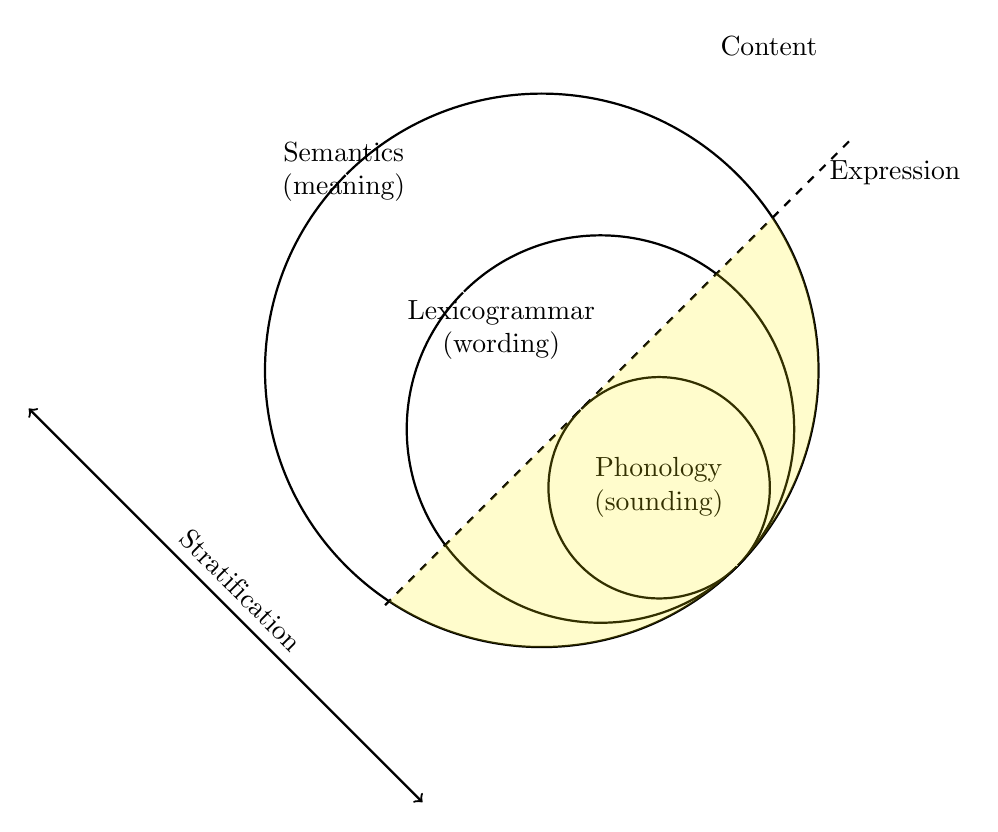
\begin{tikzpicture}
		\coordinate (o) at (0,0);
		\coordinate (o-11) at (-16em,16em);
		
		\coordinate (A) at (-9,2);
		\coordinate (C) at (-6,6);
		\coordinate (D) at (-1,1);
		
		\draw[thick, name path = mn] (o) arc(315:-360:4em);
		\draw[thick, name path = me](o) arc(315:-360:7em);
		\draw[thick, name path = mx] (o) arc(315:-360:10em);
		
		\draw[thin, white, name path = ref](o)--(o-11);
		
		\path[name intersections={of = ref and mn, name = tgt} ];
		\draw[thick, dashed, name path = plane] ($(tgt-2)!10em!90:(C)$) -- ($(tgt-2)!14em!-90:(C)$);
		\path[name intersections={of = plane and mx, name = tgt2} ];
		
		\draw[thick, <->, postaction={ decorate ,decoration = {text along path, raise=1ex, text align=center,text={Stratification}}}](A) -- +($(D)-(C)$);  % the stratification axis line
		
		\node[align = center] at (-1,1) {Phonology \\ (sounding)};
		\node[align = center] at (-3,3) {Lexicogrammar \\ (wording)};
		\node[align = center] at (-5,5) {Semantics \\ (meaning)};
		
		\node[align = center] at (2,5) {Expression};
		\node[align = center] at (0.4,6.6) {Content};
		
		\coordinate (ec) at (-0.6,2) ;
		
%		\draw[red, fill = red](tgt-1) circle(0.1em);
%		\draw[red, fill = red](tgt-2) circle(0.1em);
%		\draw[red, fill = red](tgt2-1) circle(0.1em);
%		\draw[red, fill = red](tgt2-2) circle(0.1em);
		
		%\fill[yellow, fill opacity=.4] (o) arc(315:393.5:10em) -- (tgt-2) arc (135:300:4em);
		\fill[yellow, fill opacity=.2] (o) arc(315:393.5:10em) -- (tgt2-1) arc (236.5:315:10em);
		
	\end{tikzpicture}
	\caption{The levels of abstraction along the realisation axis}
	\label{fig:stratification-sfl}
\end{figure}
 

Having that said, the stratification axis is a useful dimension to relate the formal and the systemic functional grammars. This is also an instrument employed by Hjelmslev \citep{Taverniers2011}. %TODO: eventually expand here

The SFL model defines language as a resource organised into three strata: phonology (sounding), lexicogrammar (wording) and semantics (meaning). Each is defined according to its level of abstraction on the realisation axis. The realisation axis is divided into two planes: the expression and the content planes. 
Although debate about the precise division continues, for current purpose it is sufficient to see the first stratum (i.e. phonology/morphology) belongs to the \textit{expression plane} and the last two (lexicogrammar and semantics) belong to the \textit{content plane}.
%But the division is not so clear because some parts of semantics and lexicogrammar transcend from content into expression plane. 
In this context, the formal grammar could be localised entirely within the expression plane, including the phonology/morphology, syntax, lexicon while formal semantics, stripped of any explanations in terms of the meaning potential, belongs in the content plane.

\section{Sydney theory of grammar}
\label{sec:sydney-theory-of-grammar}
I start introducing the terms of SFL theory with the Sydney grammar as this is in accordance with the historical development originating with \citet{Halliday2002} defining the categories of the theory fo grammar. He proposes four fundamental categories: \textit{unit}, \textit{structure}, \textit{class} and \textit{system}. Each of these categories is logically derivable from and related to the other ones in a way that they mutually define each other. These categories relate to each other on three scales of abstraction: \textit{rank}, \textit{exponence}, \textit{delicacy}. Halliday also uses three scale types: \textit{hierarchy}, \textit{taxonomy} and \textit{cline}.

\begin{definition}[Hierarchy]\label{def:hierarchy}
	Hierarchy [is] a system of terms related along a single dimension which involves some sort of logical precedence. 
	\citep[42]{Halliday2002}. 
\end{definition}

\begin{definition}[Taxonomy]\label{def:taxonomy}
	Taxonomy [is] a type of hierarchy with two characteristics:
	\begin{enumerate}
		\item the relation between terms and the immediately following and preceding one is constant
		\item the degree is significant and is defined by the place in the order of a term relative to following and preceding terms. \citep[42]{Halliday2002}
	\end{enumerate}
\end{definition} 

\begin{definition}[Cline]\label{def:cline}
	Cline [is] a hierarchy that instead of being made of a number of discrete terms, is a continuum carrying potentially infinite gradations.
	\citep[42]{Halliday2002}. 
\end{definition}

The concept of cline may not necessarily originate in SFL but it is used quite extensively in the domain literature.
Next I define and introduce each category of \textit{grammatics} and the related concepts that constitute the theoretical foundation for the Sydney Theory of grammar.
%TODO [JB] note how you've already lost the other three terms you had above: rank, exponence and delicacy. Either define them immediately or say where they are going to be defined.

\subsection{Unit}
\label{sec:unit-sydney}
Language is a patterned activity of meaningful organization. The patterned organization of substance (\textit{graphic} or \textit{phonic}) along a linear progression is called \textit{syntagmatic order} (or simply \textit{order}). 

\begin{definition}[Unit]\label{def:unit}
	The unit is a grammatical category that accounts for the stretches that carry grammatical patterns \citep[42]{Halliday2002}.
	The units carry a fundamental \textit{class} distinction and should be fully identifiable in description \citep[45]{Halliday2002}.
\end{definition}

\begin{generalization}[Constituency principles]\label{def:constituency-principles}
	The five principles of constituency in lexicogrammar are:
	\begin{enumerate}
		\item There is a scale or rank in the grammar of every language. That of English (typical of many) can be represented as: clause, group/phrase, word, morpheme.
		\item Each unit consists of \textit{one or more} units of rank next below.
		\item Units of every rank may form complexes.
		\item\label{item:downrank} There is potential for rank shift, whereby a unit of one rank my be down-ranked to function in a structure of a unit of its own rank or of a rank below.
		\item\label{item:unit-split} Under certain circumstances it is possible for one unit to be enclosed within another, not as a constituent but simply in such a way as to split the other into two discrete parts \citep[9--10]{Halliday2013}.
	\end{enumerate}
\end{generalization}

For example, the down-ranking (Point \ref{item:downrank}) can be observed in nominal groups that incorporate a relative clause functioning as qualifier. In example \ref{ex:downranking} \textit{that I got for Christmas} is a relative clause specifying which books are being referred. The unit split (Point \ref{item:unit-split}) can be encountered in the instances of Wh-interrogative clauses containing a preposition at the end which in fact belongs to the Wh-group. In example \ref{ex:unit-split2} the prepositional phrase \textit{Who \dots about} is gapped and has an inverted order of constituents. 

%TODO: write 2 examples here

\begin{exe}
	\ex\label{ex:downranking} I haven't read any books \textit{that I got for Christmas}.
	\ex\label{ex:unit-split2} \textit{Who} are you talking \textit{about}?
	\ex\label{ex:unit-split1} I am talking about George.
\end{exe}

The relation between units is that of consistency for which we say that a unit \textit{consists of} other units. The scale on which the units are ranged is the \textit{rank scale}. The rank scale is a levelling system of units supporting unit composition regulating how units are organised at different granularity levels from clause, to groups/phrases to words and the units of a higher rank scale consist of units of the rank next below. Table \ref{tab:rank-scale} presents a schematic representation of the rank scale and its derived complexes.

\begin{table}[h]
	\centering
	\begin{tabular}{|l|l|}
		\hline
		{\bf Rank scale $\downarrow$} & {\bf Complexing} \\ \hline
		& Clause complex           \\ \hline
		Clause           &                          \\ \hline
		& Group(/phrase) complex   \\ \hline
		Group(/phrase)   &                          \\ \hline
		& Word complex             \\ \hline
		Word             &                          \\ \hline
		& (Morpheme complex)       \\ \hline
		(Morpheme)       &                          \\ \hline
	\end{tabular}
	\caption{Rank scale of the (English) lexicogrammatical constituency}
	\label{tab:rank-scale}
\end{table}

\begin{generalization}[Rank scale constraints]\label{def:rank-skale-constraints}
	The rank relations are constrained as follows:
	\begin{enumerate}
        \item in general elements of clauses are filled by groups,the elements of groups by words and the elements of words by morphemes.
		\item downward \textit{rankshift} is allowed i.e. the transfer of a given unit to a lower rank. 
		\item upward rankshift is not allowed.
		\item only whole units can enter into higher units \citep[44]{Halliday2002}.
	\end{enumerate}
\end{generalization}

The Generalization \ref{def:rank-skale-constraints} taken as a whole means that a unit can include, in what it consists of, a unit of rank higher than or equal to itself but not a unit of rank more than one degree lower than itself; and not in any case a part of any unit \citep[42]{Halliday2002}. 

Following the rank scale constraints above the concept of embedding can be defined as follows. 

\begin{definition}[Embedding]\label{def:embedding0}
    Embedding is the mechanism whereby a clause or phrase comes to function as a constituent within the structure of a group, which is itself a constituent of a clause. \citep[242]{Halliday2013}
\end{definition}

Halliday states that embedding is a phenomena that occurs only when a phrase/group or clause function within the structure of a group which is itself a constituent of a clause \citep[242]{ifg2}. The above definition of embedding permits the only for a clause and groups that function as elements of groups which means that a clause cannot fill the elements of another clause \citep[237]{Fawcett2000}.

\subsection{Structure}
%TODO: Top down is good for generation and bottom up for parsing
%TODO: agnation as a clive vs instanciation as a cline | subclassification rel vs class-instance rel
%TODO: Rebekah Wegener PhD SFL thesis online [Parameters of context]: Chapter in SFL theory 

\begin{definition}[Structure]\label{def:structure}
	The structure (of a given unit) is the arrangement of \textit{elements} that take places distinguished by the order relationship \citep[46]{Halliday2002}.
\end{definition}

\begin{definition}[Element]\label{def:element}
	Element is defined by the place stated as absolute or relative position in sequence and with reference to the unit next below \citep[47]{Halliday2002}. 
\end{definition}


\begin{figure}[h]
	\begin{tikzpicture}
		\tikzset{
			rect/.style n args={4}{
				draw=none,
				rectangle,
				append after command={
					\pgfextra{%
						\pgfkeysgetvalue{/pgf/outer xsep}{\oxsep}
						\pgfkeysgetvalue{/pgf/outer ysep}{\oysep}
						\def\arg@one{#1}
						\def\arg@two{#2}
						\def\arg@three{#3}
						\def\arg@four{#4}
						\begin{pgfinterruptpath}
						\ifx\\#1\\\else
						\draw[draw,#1] ([xshift=-\oxsep,yshift=+\pgflinewidth]\tikzlastnode.south east) edge ([xshift=-\oxsep,yshift=0\ifx\arg@two\@empty-\pgflinewidth\fi]\tikzlastnode.north east);
						\fi\ifx\\#2\\\else
						\draw[draw,#2] ([xshift=-\pgflinewidth,yshift=-\oysep]\tikzlastnode.north east) edge ([xshift=0\ifx\arg@three\@empty+\pgflinewidth\fi,yshift=-\oysep]\tikzlastnode.north west);
						\fi\ifx\\#3\\\else
						\draw[draw,#3] ([xshift=\oxsep,yshift=0-\pgflinewidth]\tikzlastnode.north west) edge ([xshift=\oxsep,yshift=0\ifx\arg@four\@empty+\pgflinewidth\fi]\tikzlastnode.south west);
						\fi\ifx\\#4\\\else
						\draw[draw,#4] ([xshift=0+\pgflinewidth,yshift=\oysep]\tikzlastnode.south west) edge ([xshift=0\ifx\arg@one\@empty-\pgflinewidth\fi,yshift=\oysep]\tikzlastnode.south east);
						\fi
						\end{pgfinterruptpath}
					}
				}
			}, 
			unit/.style={rect={draw=black, thick}{draw=black, thick}{draw=black, thick}{}},
			place/.style = {rect={draw=black, thick}{}{draw=black, thick}{draw=black, thick}, text width=5.5em,},
			}
		
		\node[unit, text width=\textwidth,align=center](unit-line){};
		\node[above = 0.1em of unit-line](unit-label){Unit};
		%place lines
		{[start chain=l going left,node distance=1em]
			\node[on chain=l,place, below =3em of unit-line](p1){};
			\node[on chain=l,place](p2){};
			\node[on chain=l,place](p3){};
		}
		%place lines to the right
		{[start chain=r going right, node distance=1em,]
			\node[on chain=r,place, right = 1em of p1.east](p4){};
			\node[on chain=r,place](p5){};
			}
		%place labels
		\node[below=0.1em of p1](l3){place_{3}};
		\node[below=0.1em of p2](l2){place_{2}};
		\node[below=0.1em of p3](l1){place_{1}};
		\node[below=0.1em of p4](l4){place_{4}};
		\node[below=0.1em of p5](l5){place_{5}};
		%functional elements
		\node[above = 0.4em of p1, align=center, rectangle, draw, thick,dashed](element1){functional\\element_{3}};
		\node[above = 0.4em of p2, align=center, rectangle, draw, thick,dashed](element2){functional\\element_{2}};
		\node[above = 0.4em of p3, align=center, rectangle, draw, thick,dashed](element3){functional\\element_{1}};
		\node[above = 0.4em of p4, align=center, rectangle, draw, thick,dashed](element4){functional\\element_{4}};
		\node[above = 0.4em of p5, align=center, rectangle, draw, thick,dashed](element5){functional\\element_{5}};
		%order relations
		\draw[bend right,<->,dashed]  (l1) to node [below] {order} (l2);
		\draw[bend right,<->,dashed]  (l2) to node [below] {order} (l3);
		\draw[bend right,<->,dashed]  (l3) to node [below] {order} (l4);
		\draw[bend right,<->,dashed]  (l4) to node [below] {order} (l5);
	\end{tikzpicture}
	\caption{The graphic representation of (unit) structure}
	\label{fig:structure-representation}
\end{figure}

We say that a unit is composed of elements located in places and that its internal structure is accounted for elements in terms of functions and places taken by the lower (constituting) units or lexical items. The graphic representation of the unit structure is depicted in Figure \ref{fig:structure-representation}. The unit structure is referred in linguistic terminology as \textit{constituency} (whose principles are enumerated in Generalization \ref{def:constituency-principles}). In the unit structure, the elements resemble an array of empty slots that are \textit{filled} by other units or lexical items.

For example to account for the English clause structure four elements are needed: \textit{subject}, \textit{predicator}, \textit{complement} and \textit{adjunct}. They yield the distinct symbols, so that S, P, C, A is the inventory of elements. They then can be arranged in various orders falling in particular places, say SPC, SAPA, ASPCC etc. The places of elements are important with respect to the structure of the whole unit but also with respect to the relative ordering between these elements. For example S always fronts P, C is fronted by P unless the clause realises a Wh-interrogative whereas A is quite free and can occur anywhere in the unit structure. 

\subsection{Class}

To one place in the structure corresponds one occurrence of the unit next below. This means that there will be a certain grouping of members identified by the functional element they take in the structure. Patterning such groupings leads to emergence of \textit{classes} of units.

In the clause structure example, elements in the unit are occupied by units of lower rank and of a particular class. The relation between the element and the class is mutually determined. In each of these elements is placed a lower rank unit and of an expected class. For instance in the S position can be placed a \textit{noun}, \textit{nominal group}, \textit{pronoun} or another \textit{clause} (that will be a down-ranking situation defined above).

\begin{definition}[Class]\label{def:class}
	The class is that grouping of members of a given unit which is defined by the operation (i.e. functional element) in the structure of the unit next above \citep[49]{Halliday2002}.
\end{definition}

Halliday defines class (Definition \ref{def:class}) as likeness of the same rank \textit{phenomena} to occur together in the structure. He adopts a top-down approach stating that the class of a unit is determined by the \textit{function} (Definition \ref{def:function}) it plays in the unit above and not by its internal structure of elements. In SFG the structure of each class is well accounted in terms of syntactic variation recognizing six unit classes: \textit{clause}, \textit{nominal}, \textit{verbal}, \textit{adverbial} and \textit{conjunction} groups and \textit{prepositional phrase}. The Sydney grammar unit structure model is briefly summarised in the Appendix \ref{ch:syntax-overview}.

\subsection{System}
\label{sec:system}
As described above, structure is a syntagmatic ordering in language capturing regularities and patterns which can be paraphrased as \textit{what goes together with what}. However in SFG most of the descriptive work is carried not syntagmatically but paradigmatically via \textit{system networks} (Definition \ref{def:system}) describing \textit{what could go instead of what} \citep[22]{Halliday2013}. Note that the paradigmatic-syntagmatic axes date back to the works of \citet{Saussure15}. Both are important for completing a linguistic description. Here lies one of the main differences between SFL and other approaches which is is taking the paradigmatic path whereas many others take the syntagmatic path to language representing it as an inventory of structures. 
%An essential assumption of systemicists is that the language is best represented in the form of system networks and not as an inventory of structures. 
The structure of course is a part of language description but it is only a syntagmatic manifestation of the systemic choices and one needs to account for both \citep[23]{Halliday2013}.

\begin{definition}[System]\label{def:system}
	A system is a set of mutually exclusive set of terms referring to meaning potentials in language and are mutually defining. The system is considered self-contained, closed and complete with the following characteristics:
	\begin{enumerate}
		\item the number of terms is finite,
		\item each term is exclusive of all others,
		\item if a new term is added to the system it changes the meaning of all the other terms \citet[41]{Halliday2002}.
	\end{enumerate}
\end{definition}

The concept of a system as presented in Definition \ref{def:system} has its roots in the works of \citet{Saussure15} and \citet{Hjelmslev53} and Halliday only cements it in SFL architecture of grammar.

Going back to the notion of class previously defined as a grouping of items identified by functions in the structure, it needs stressed here that class is not a list of formal items but an abstraction from them. By increase in \textit{delicacy} a class is broken into secondary classes. 

\begin{definition}[Delicacy]\label{def:delicacy-sydney}
	Delicacy is the scale of differentiation or depth of detail whose limit at one end is the primary degree of categories of structure  and class and on the other end, theoretically, is the point beyond which no further grammatical relations obtain. \citet[58]{Halliday2002}  
\end{definition}

We say that a category is refined into more subtle distinctions of subcategories which form a system as define above. Subsequently those distinctions fo subcategories can be further refined in other systems. This relationship between these two systems is one of delicacy where the second one is more delicate than the first one and together they form a \textit{system network}. As a side note, the delicacy in a system network is akin to sub-classification relation, which was originally the intended one and the predominant one. In practice, however, a few kinds of abstraction relations can be encountered as there are multiple kinds of abstraction (e.g abstraction as information reduction, or as approximation, or as idealisation etc.) that are extensively treated by \citet{Saitta2013}. This discussion however is not in the scope of the current work.

%%%
The graphical notations introduced by \citet{Halliday2013} are useful in reading and writing system networks in this thesis. Below is a system network with a simple \textit{entry condition} (Figure \ref{fig:system-network-notation1}), a \textit{system network grouping} that share the same entry condition (Figure \ref{fig:system-network-notation2}), a system network with a \textit{disjunctive} and \textit{conjunctive} entry conditions (Figure \ref{fig:system-network-notation3} and \ref{fig:system-network-notation4}). 
%%%%%%%%%%%%%%%%%%%%%%%%%%%%%%%%%
\begin{figure}[H]
    \centering
    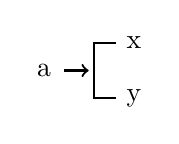
\begin{tikzpicture}[]
    \node (prec) [system-name] {a};
    \node (f1) [system-name, right = 2em of prec, yshift=1em] {x};
    \node (f2) [system-name, right = 2em of prec, yshift=-1em] {y};
    %\draw [decorate,decoration={brace,amplitude=3em},xshift=-4pt,yshift=0pt] ([xshift=0.0em] f1.west) -- (f2.west) node [black,midway,xshift=-0.6cm] {qwe}; 
    \draw [thick] ([xshift=-0.0em] f1.west) to [square right brace ] ([xshift=-0.0em] f2.west);
    \draw[precondition] ([xshift=0.1em] prec.east) -- ([xshift=1.0em,yshift=0em] prec.east);
    \end{tikzpicture}
    \caption{A system with a single entry condition: if \textit{a} then either \textit{x} or \textit{y}}
    \label{fig:system-network-notation1}
\end{figure}

\begin{figure}[H]
    \centering
    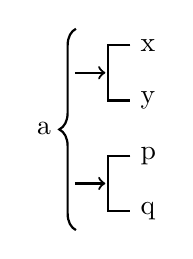
\begin{tikzpicture}[]
    \node (prec) [system-name] {a};
    \node (f1) [system-name, right = 2.5em of prec, yshift=3em] {x};
    \node (f2) [system-name, right = 2.5em of prec, yshift=1em] {y};
    
    \node (f3) [system-name, right = 2.5em of prec, yshift=-1em] {p};
    \node (f4) [system-name, right = 2.5em of prec, yshift=-3em] {q};
    
    \draw [thick] ([xshift=-0.0em] f1.west) to [square right brace ] ([xshift=-0.0em] f2.west);
    \draw [thick] ([xshift=-0.0em] f3.west) to [square right brace ] ([xshift=-0.0em] f4.west);
    
    \draw [decorate,thick, decoration={brace, amplitude=0.6em},xshift=0pt,yshift=0pt] ([xshift=-2.6em] f4.south) -- ([xshift=-2.6em] f1.north);
    
    \draw[precondition] ([xshift=0.5em, yshift=2em] prec.east) -- ([xshift=1.6em, yshift=2em] prec.east);
    \draw[precondition] ([xshift=0.5em, yshift=-2em] prec.east) -- ([xshift=1.6em, yshift=-2em] prec.east);
    \end{tikzpicture}
    \caption{Two systems grouped under the same entry condition: if \textit{a} then both either \textit{x} or \textit{y} and, independently, either \textit{p} or \textit{q}}
    \label{fig:system-network-notation2}
\end{figure}

\begin{figure}[H]
    \centering
    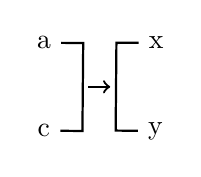
\begin{tikzpicture}[]
    \node (prec1) [system-name] {a};
    \node (prec2) [system-name, below=2em of prec1] {c};
    
    \draw [thick] ([xshift=-0.0em] prec1.east) to [square left brace ] ([xshift=-0.0em] prec2.east);
    \draw[precondition] ([xshift=1.6em, yshift=-1em] prec1.south) -- ([xshift=2.4em, yshift=-1em] prec1.south);
    
    \node (f1) [system-name, right =2.8em of prec1] {x};
    \node (f2) [system-name, right =2.8em of prec2] {y};
    
    \draw [thick] ([xshift=-0.0em] f1.west) to [square right brace ] ([xshift=-0.0em] f2.west);
    
    \end{tikzpicture}
    \caption{A system network with a disjunctive entry condition: if either \textit{a} or \textit{c} (or both), then either \textit{x} or \textit{y}}
    \label{fig:system-network-notation3}
\end{figure}

\begin{figure}[H]
    \centering
    \begin{tikzpicture}[]
    \node (prec1) [system-name] {a};
    \node (prec2) [system-name, below=4em of prec1] {b};
    
    \node (f1) [system-name, right =5em of prec1, yshift=-1em] {x};
    \node (f2) [system-name, right =5em of prec2, yshift=1em] {y};
    
    \draw [thick] ([xshift=-0.0em] f1.west) to [square right brace ] ([xshift=-0.0em] f2.west);
    
    \draw [decorate,thick, decoration={brace, amplitude=0.6em},xshift=0pt,yshift=0pt] ([xshift=-4.0em, yshift=-0.6em] f1.north) -- ([xshift=-4.0em, yshift=0.6em] f2.south);
    
    \draw[precondition] ([xshift=3.2em, yshift=-2.1em] prec1.south) -- ([xshift=4.1em,yshift=-2.1em] prec.south);
    
    \draw[thick] (prec1.south east) -- ([xshift=1.5em, yshift=-1.8em] prec1.east);
    \draw[thick] (prec2.north east) -- ([xshift=1.5em, yshift=1.8em] prec2.east);
    
    \end{tikzpicture}
    \caption{A system with a conjunctive entry condition: if both \textit{a} and \textit{b} then, either \textit{x} or \textit{y}}
    \label{fig:system-network-notation4}
\end{figure}
%%%%%%%%%%%%%%%%%%%%%%%%%%%%%%%%%

%TODO example of polarity system from IFG4 p23

It is worth noting that when a piece of language is analysed, it can be approached at various levels of delicacy. We say that delicacy is variable in description, and one may choose to provide coarse grained analysis without going beyond primary grammatical categories or it can dive into fine grained categorial distinctions, still being comprehensive with regards to the rank, \textit{exponence} and grammatical categories. 

\begin{definition}[Exponence]\label{def:exponence-sydney}
    Exponence is the scale which relates the categories of theory which are with high degree of abstraction to formal items on its low end. Each exponent can be linked directly to the formal item or by taking successive steps on the exponence scale and changing rank where necessary. \citet[57]{Halliday2002}
\end{definition}

And in relation to the previous section, the class stand in the relation of exponence to an element of primary structure of the unit next above. This breakdown gives a system of classes that constitute choices implied by the nature of the class \citep[41]{Halliday2002}. 



\subsection{Functions and metafunction}
Above, when talking about structure, I described a unit as being composed of elements accounted in terms of \textit{functions} and places taken by the lower (constituting) units or lexical items.

\begin{definition}[Function]\label{def:function}
	The functional categories or functions provide an interpretation of grammatical structure in terms of the overall meaning potential of the language. \citep[76]{Halliday2013}.
\end{definition}

Most constituents of clause structure, however, have more than one function, which is called a \textit{conflation of elements}. For example in the sentence ``Bill gave Dolly a rose'', ``Bill'' is the Actor doing the act of giving but also the Subject of the sentence. So we say that Actor and Subject functions are conflated in the constituent ``Bill''. This is the concept of \textit{metafunction} or \textit{strand of meaning} comes into the picture. The Subject function is said to belong to the \textit{interpersonal metafunction} while the Actor function belongs to the \textit{experiential metafunction}. 

Halliday identifies three fundamental dimensions of structure in the clause, each meaning: \textit{experiential}, \textit{interpersonal} and \textit{textual}. He refers to them as \textit{metafunctions} and they account for the functions that language units take on in communication. Table \ref{tab:metafucntions} presents the metafunctions and their reflexes in grammar as proposed by  \citet[85]{Halliday2013}.

\begin{table}[H]
	\centering
	\begin{tabulary}{\textwidth}{|l|L|L|L|}
		\hline
		{\bf Metafunction} & {\bf Definition(kind of meaning)} & {\bf Corresponding status in clause} & {\bf Favored type of structure}   \\ \hline
		experiential       & construing a model of experience  & clause as representation             & segmental (based on constituency) \\ \hline
		interpresonal      & enacting social relationship      & clause as exchange                   & prosodic                          \\ \hline
		textual            & creating relevance to context     & clause as message                    & culminative                       \\ \hline
		logical            & constructing logical relations    & complexes (taxis \& logico-semantic type) & iterative                         \\ \hline
	\end{tabulary}
	\caption{Metafunctions and their reflexes in the grammar}
	\label{tab:metafucntions}
\end{table}

Across the rank scale, with respect to structure and metafunctions, Halliday formulates the general principle of \textit{exhaustiveness} (Generalization \ref{def:exhaustiveness}) saying that clause constituents have at least one and may have multiple functions in different strands of meaning; however this does not mean that it must have a function in each of them. For example interpersonal Adjuncts such as ``perhaps'' ot textual Adjuncts such as ``however'' play no role in the clause as representation. 

\begin{generalization}[Exhaustiveness principle]\label{def:exhaustiveness}
    Everything in the wording has some function at every rank but not everything has a function in every dimension of structure \citep{Halliday2002,Halliday2013}.
\end{generalization}

This principle implicitly relates to the property of language meaning that 
%it naturally evolves towards the shortest and most effective way of expressing a meaning. 
there is nothing meaningless and thus every piece of language must be explained and accounted for in the lexicogrammar. 

At the very top of the rank scale, clauses form complex structures. Halliday employs systematically the concepts of \textit{taxis} and \textit{logico-semantic relations} to account for inter-clausal relations. 

\begin{definition}[Taxis]\label{def:taxis}
    \textit{Taxis} represents the degree of interdependency between units systematically arranged in a linear sequence where \textit{parataxis} means equal and \textit{hypotaxis} means unequal status of units forming a \textit{nexus} together.
\end{definition}

Of importance here is the concept of taxis which is very useful at describing unit relations not only at the group and clause ranks but all the way down to smallest linguistic unit such as morphemes and phonemes. I will also refer to it when describing the Cardiff theory of grammar and also briefly in the discussion of dependency relations in Section \ref{sec:cross-theoretical-bridge}. 

\subsection{Lexis and lexicogrammar}
In SFL the terms \textit{word} and \textit{lexical item} are not really synonymous. They are related but they refer to different things. The term \textit{word} is reserved (in early Halliday) for the grammatical unit of the lowest rank whose \textit{exponents} are lexical items. %While word refers to the unit of structure below the group/phrase rank and above the morphemes, the lexical item is defies as follows. 

\begin{definition}[Lexical Item]\label{def:lexical-item}
	In English, a lexical item may be a \textit{morpheme}, \textit{word} (in traditional sense) or \textit{group (of words)} and it is assigned to no rank \citep[60]{Halliday2002}.
\end{definition}

Examples of lexical items are the following: ``'s'' (the possessive morpheme), ``house'', ``walk'', ``on'' (words in traditional sense) and ``in front of'', ``according to'', ``ask around'', ``add up to'', ``break down'' (multi word prepositions and phrasal verbs).

If some theories treat grammar and lexis as discrete phenomena, Halliday brings them together as opposite poles of the same cline. He refers to this merge as \textit{lexicogrammar} where they are paradigmatically related through delicacy relation.
% and he expressed his dream that one day linguists will be able to turn whole linguistic form into (lexico)grammar showing that lexis is the most delicate grammar. 
\citet{Hasan2014}, explores the feasibility of what would it mean to turn the ``whole linguistic form into grammar''. This then implies a assumption that lexis is not form and that its relation to semantics is unique which  in turn is challenging the problems of polysemy. 


%%%%%%%%%%%%%%%%%%%%%%%%%%%%%%%%%%%%%%%%%%%%%%%%%%%%%%%%%%%%%%%%%
\section{The Cardiff theory of grammar}
\label{sec:cardiff-theory-grammar}
As presented in the introduction and explained by \citet{Bateman2008}, the accounts along the syntagmatic axis had gone missing in the Sydney grammar leaving unresolved how to best represent the structure of language at the level of form. This section present the theory of systemic functional grammar as conceived by Robin Fawcett at the University of Cardiff. His book ``A theory of syntax for Systemic Functional Linguistics'' \citep{Fawcett2000} presented a proposal for a \textit{unified syntactic model} for SFL that contrasts several aspects of Hallidayan grammar but share the same set of fundamental assumptions about the language; it is an extension and a simplification in a way.

Fawcett questions the status of multiple structures in the theory and whether they can finally be integrated into a simpler sole representation. A big difference to Hallidayan theory is renouncing the concept of rank scale which has an impact on the whole theory. Another is the bottom-up approach to unit definition as opposed to top-down one advocated by Halliday. These two and a few other differences have important implications for the overall theory of grammar and consequently for the grammar itself. As a consequence, to accommodate the lack of rank-scale, Fawcett adapts the definitions of the fundamental concepts and changes his choice of words (for example ``class'' and ``unit'' turn into ``class of unit'' treated as one concept rather than two distinct ones).

\citet{Fawcett2000} proposes three fundamental categories in the theory of grammar: \textit{class of unit}, \textit{element of structure} and \textit{item}. Constituency is a relation accounting for the prominent compositional dimension of language. However a unit does not function directly as a constituent of another unit but via a specialised relation which Fawcett breaks down into three sub-relations: \textit{componence}, \textit{filling} and \textit{exponence}. Informally it is said that a unit is composed of elements which are either filled by another unit or expounded by an item. He also proposes three secondary relations of \textit{coordination}, \textit{embedding} and \textit{reiteration} to account for a more complete range of syntactic phenomena.

\subsection{Class of units}
Fawcett's theory of language assumes a model with two levels of \textit{meaning} and \textit{form} corresponding to \textit{semantic units} and \textit{syntactic units} which are mutually determined (which is the case for any sign in a Saussurean approach to language). 

\begin{definition}[Class of Unit]\label{def:class2}
	The class of unit [...] expresses a specific array of meanings that are associated with each one of the major classes of entity in semantics [...and] are to be identified by the elements of their internal structure \citep[195]{Fawcett2000}. 
\end{definition}

For English Fawcett proposes four main kinds of semantic entities: situations, things, qualities (of both situations and things) and quantities. Each of these semantic units corresponds to five major classes of syntactic units: \textit{clause}, \textit{nominal group}, \textit{prepositional group}, \textit{quality group} and \textit{quantity group}. In addition he recognises two more minor classes i.e. the \textit{genitive cluster} and the \textit{proper name cluster} \citep[193--194]{Fawcett2000}. 

%He proposes that in English there are four major semantic classes of entities: situations, things, qualities (of situations and things) and quantities (typically of things but also of situations and qualities) corresponding to major syntactic units of \textit{clause}, \textit{nominal group}, \textit{prepositional group}, \textit{quality group} and \textit{quantity group} along with a set of minor classes such as \textit{genitive cluster} and \textit{proper name cluster}  \citep[193--194]{Fawcett2000}. 

Fawcett's classification is based on the idea that the syntactic and semantic units are mutually determined and supported by grammatical patterns. However those patterns lie beyond the syntactic variations of the grammar and so blend into lexical semantics.

In Sydney theory the class is determined by the function it plays in the unit above. By contrast, in Cardiff theory, the class of unit is determined based on its internal structure i.e. by its \textit{elements of structure} (and not by the function it plays in the parent unit).  

\subsection{Element of structure}
\label{sec:elements-of-structure}

The terms \textit{element} and \textit{structure} have roughly the same meaning as defined in Sydney theory of grammar (defined in Section \ref{sec:sydney-theory-of-grammar}) but with two additional stipulations presented below.

\begin{definition}[Element of Structure]\label{def:elementStructure}
	Elements of structure are immediate components of classes of units and are defined in terms of their \textit{function} in expressing meaning and not in terms of their absolute or relative position in the unit. \citep[213--214]{Fawcett2000}. 
\end{definition}

The definition above leads as a consequences to two important properties of elements formulated as follows.

\begin{generalization}[Element functional uniqueness]
Every element in a given class of unit serves a function in that unit different from the function of the sibling elements \citep[214]{Fawcett2000}. 
\end{generalization} 

Even if for example, different types of \textit{modifiers} in English nominal group seem to have very slight differences in functions, they are still there.

\begin{generalization}[Element descriptive uniqueness]
    Every element in every class of unit will be different from every element in every other class of unit \citep[214]{Fawcett2000}. 
\end{generalization} 

Thus the terms of modifier and head shall not be used for more than one class of unit. In English grammar the head and modifier are used for nominal group only. And in other groups the elements of structure may seem similar to modifier and head, they still receive different names such as \textit{apex} and \textit{temperer} in the quality group.

The elements (of structure) are functional slots which define the internal structure of a unit but still they are \textit{located} in \textit{places}. One more category that intervenes between element and unit is the concept of \textit{place} which become essential for the generative versions of grammar.

There are two ways to approach place definition. The first is to treat places as positions of elements relative to each other (usually previous). This leads to the need for an \textit{anchor} or a \textit{pivotal element} which may not always be present/realised.

The second is to treat places as a linear sequence of locations at which elements may be located, identified by numbers ``place 1'', ``place 2'' etc. This place assignment approach is absolute within the unit structure and makes elements independent of each other. This approach has been used in COMMUNAL \citep{Fawcett90-communal} and PENMAN \citep{PenmanOverview} projects. 

\subsection{Item}
\begin{definition}[Item]\label{def:item}
	The item is a lexical manifestation of meaning outside syntax corresponding to both words (in the traditional sense), morphemes and either intonation or punctuation (depending whether the text is spoken or written). \citep[226--232]{Fawcett2000}. 
\end{definition}

Items correspond to the leaves of syntactic trees and constitute the raw \textit{phonetic} or \textit{graphic} manifestation of language. The collection of items of a language is generally referred to as \textit{lexis}.

Since items and units are of different natures, the relationship between an element and a (lexical) item must be different from that to a unit. We say that items \textit{expound} elements and not that they \textit{fill} elements as units do. 

\begin{definition}[Exponence (restricted)]\label{def:exponence}
    Exponence is the relation by which an element of structure is realised by a (lexical) item \citep[254]{Fawcett2000}. 
\end{definition}

If in Sydney model exponence (Definition \ref{def:exponence-sydney}) is a relation that links abstract grammatical categorise to the data In Cardiff model it has a restricted meaning referring to relation between items and elements only. 

\subsection{Componence and obscured dependency}
\label{sec:componence}
\begin{definition}[Componence]\label{def:componence}
    Componence is the part-whole relationship between a unit and the elements it is composed of \citep[244]{Fawcett2000}. 
\end{definition}

Note that componence is not a relationship between a unit and its places; the latter, as discussed in Section \ref{sec:elements-of-structure}, simply locationally relate elements of a unit to each other.

Componence intuitively implies a part-whole constituency relationship between the unit and its elements. But this is not the only view. Another perspective is the concept of \textit{dependency} (which I will address in Chapter \ref{ch:dependecy-grappamr}) or strictly speaking the \textit{sister} or \textit{sibling dependency} (not parent-daughter). 
It is suitable for describing relations between elements of structure within a unit. 

\begin{exe}
    \ex\label{ex:the-man-with-a-stick} the man with a stick
\end{exe}

For example the componence of nominal group in Example \ref{ex:the-man-with-a-stick} is (\textit{dd h q}) which are symbols for (\textit{determiner head qualifier}). The same can be expressed in terms of sibling dependency relations depicted in Figure \ref{fig:dep-example-man-with-a-stick}. The relations from \textit{stick} to \textit{with a} are not depicted because they belong in description of prepositional group \textit{with a stick}.

\begin{figure}[!ht]
    \centering
    \begin{dependency}[dep-style]
        \begin{deptext}[column sep=1em]
            (the \& man \& ( with \& a \& stick )) \\
        \end{deptext}
        \deproot{2}{ROOT}
        \depedge[edge unit distance =1em]{2}{1}{dd}
        \depedge[edge unit distance =0.333em]{2}{5}{q}
    \end{dependency}
	\caption{Sibling dependency representation for ``the man with a stick''}
    \label{fig:dep-example-man-with-a-stick}
\end{figure}

In both SFL theories, the sister dependency relations is considered a by-product or second order concept that can be deduced from the constituency structure thus unnecessary in the grammar model. I will come back to this point because current work relies on this dual view on elements of structure and relation to the whole unit. 

The (supposed) dependency relation between a modifier and the head, in the framework of SFG is, not a direct one. 
% that form-centred linguists consider to be
Simply assume that what modifier modifies is the head. Here, however, the general function of the modifiers is to contribute to the meaning of the whole unit which is anchored by the head. 
%TODO Introduce the concept of pivotal element

In the nominal group from Example \ref{ex:the-man-with-a-stick}, the \textit{determiner} and \textit{qualifier} are modifiers that contributes to the description of the referent stated by the \textit{head}. So the head realises one type of meaning that relates the \textit{referent} while modifier realises another one. Both of them describe the referent via different kinds of meaning, therefore, according to Fawcett, they are related indirectly to each other because the modifier does not modify the head but the referent denoted by the head From this point of view, whether the element is dependent on a sibling element such as the head or on the parent unit is beside the point because in syntax we can observe its realization in system networks \citep[216--217]{Fawcett2000}.
Next I move towards last concept in Cardiff model, that of \textit{filling}, which is a relation between the elements of structure and the units below.

\subsection{Filling and the role of probabilities}
\begin{definition}[Filling]\label{def:filling}
    Filling is the probabilistic relationship between a element and the unit lower in the tree that operates at that element \citep[238, 251]{Fawcett2000}. 
\end{definition}

Fawcett replaces the rank scale with the concept of \textit{filling probabilities}. The probabilistic predictions are made in terms of filling relationship between a unit and an element of structure in a higher unit in the tree rather than being a relationship between units of different ranks. This moves focus away from the fact that a unit is for example a group, and towards what group class it is. 

In this line of thought, some elements of a clause are frequently filled by groups, but some other elements are rather \textit{expounded} by items. The frequency varies greatly and is an important factor for predicting or recognizing either the unit class or the element type in the filling relationship. 

Filling may add a \textit{single unit} to the element of structure or it can introduce \textit{multiple coordinated units}. Coordination (Example \ref{ex:coordination}) is usually marked by an overt \textit{Linker} such as \textit{and}, \textit{or}, \textit{but}, etc. and sometimes is enforced by another linker that introduces the first unit such as \textit{both}.

\begin{definition}[Coordination]\label{def:coordination}
    Coordination is the relation between units that fill the same element of structure \citep[263]{Fawcett2000}. 
\end{definition}

\begin{exe}
    \ex\label{ex:coordination} she is (friendly, nice and polite)
    \ex\label{ex:reiteration} she is (very very) nice!
\end{exe}

Coordination is through by Fawcett as being not between syntactic units but between mental referents. It always introduces more than one unit which are syntactically and semantically in similar (somehow) resulting in a \textit{syntactic parallelism} which often leads to \textit{ellipsis}. 

\begin{definition}[Reiteration]\label{def:reiteration}
    Reiteration is the relation between successive occurrences of the same item expounding the same element of structure  \citep[271]{Fawcett2000}. 
\end{definition}

Reiteration (Example \ref{ex:reiteration}) often is used to create the effect of emphasis. Like coordination, reiteration is a relation between entities that fill the same element of the unit structure which is problematic in my opinion and I further discuss it in Section \ref{sec:coordination}.

Filling also makes possible the embedding relation  which Fawcett treats as a general principle in contrast to more specific Definition \ref{def:embedding0} from Sydney model.

\begin{definition}[Embedding (generic)]\label{def:embedding}
    Embedding is the relation that occurs when a unit fills (directly or indirectly) an element of the same class of units; that is when a unit of the same class occurs (immediately) above it in the tree structure \citep[264]{Fawcett2000}. 
\end{definition}

\begin{exe}
    \ex\label{ex:embedding-direct} (To become an opera singer) takes years of training.
    \ex\label{ex:embedding-indirect} The girl (whom he is talking to) is an opera singer.
\end{exe}

In Example \ref{ex:embedding-direct} we can see an occurrence of direct embedding where an infinite clause acts as the subject of another clause. In Example \ref{ex:embedding-indirect} the embedding is indirect as the relative clause is part of the nominal group which functions as the subject in the parent clause. In both cases we say that a lower clause is embedded (directly or indirectly) in higher or parent clause. I will further discuss this in the context of rank-scale concept in Section \ref{sec:rank-system}.

A situation converse to reiteration and coordination where a element is filled by more than one unit, is known as \textit{conflation} where a unit can take more than one function within another. 

\begin{definition}[Conflation]\label{def:conflation}
    Conflation is the relationship between two elements that are filled by the same unit having the meaning of ``immediately after and fused with'' and function as one element \citep[249--250]{Fawcett2000}. 
\end{definition}

Conflation is useful in expressing multi-faceted nature of language when for example syntactic and semantic elements/functions are realised by the same unit. For example the Subject ``the girl whom he is talking to'' is also a \textit{Carrier} while the Complement ``an opera singer'' is also an \textit{Attribute}. Also conflation relations frequently occur between syntactic elements as well such as for example the \textit{Main Verb} and \textit{Operator} or \textit{Operator} and \textit{Auxiliary Verb}.

% taxis
Both, coordination and embedding relations make it possible to deal without inter-clausal \textit{hypotaxis} and \textit{parataxis} relations described in Sydney Grammar.

%
Note also that filling and componence are two complementary relations that occur in the syntactic tree down to the level when the analysis moves out of abstract syntactic categories to more concrete category of items via the relationship of exponence.

%\section{Critical discussion on the categories of the theory of grammar: a conciliation of the two theories}
\section{Critical discussion on both theories}

The two sections above cover the definitions and fundamental concepts from each of the two systemic functional theories of grammar. The work in this thesis uses a mix of concepts from both theories and this section discusses in detail what is being adopted and why attempting a rather pragmatic reconciliation for the purposes of achieving a parsing system than a theoretical debate. Next I draw parallels and highlight correspondences between the Sydney and Cardiff theories of grammar and where alter and present my position on the matter. 

\subsection{Relaxing the rank scale}
\label{sec:rank-system}
%TODO: it is problemantic the fact that when switching metafunction we get a switch in the rank scale for a primary unit of analisys
%TODO: diconnect syntax and metafunctions.
%TODO: metafunctional dimesion breaks down when we look at the context

The \textit{rank scale} proposed by \citet{Halliday2002} became over time a highly controversial concept in linguistics. The discussion whether it is suitable for grammatical description or not still continues. The historic development of this debate is documented in some detail \cite[309--338]{Fawcett2000}. %Some strong opponents of the rank scale are Hudson, Huddleston and Fawcett.

%The hierarchy of scale varies across languages and for English there are only three levels: clause, group and word. At each rank level of the scale each unit shall be unambiguously described so that it can be identified and distinguished from others. This is the \textit{``total accountability''} principle seems attainable from the descriptive perspective however is quite difficult to fulfil in generative terms.

%%TODO[JB] No: say what the problems are and how you fix them. If it is too rigid, *show* that it is too rigid. If that is what you are going to do now, *say* that you are going to show/argue this: do not simply state that it is 'too rigid' before having done the work (of discussing).
%I consider rank scale a very useful dimension for unit classification and placement but the definition laid by the Sydney school is too rigid and thus I propose to relax it into a weaker version of it. The relaxation consists of dropping completely the \textit{rank scale constraints} as enunciated in Generalization \ref{def:rank-skale-constraints}. An immediate consequence is that the \textit{embedding} relation can be broadly defined as a naturally occurring phenomena in language at all ranks and not only for clauses as initially proposed.

In this section I present a few cases that highlighting when the rank scale as defined by Sydney is too rigid. As a consequence for the purpose of thesis I drop the \textit{rank scale constraints} as enunciated in Generalization \ref{def:rank-skale-constraints}. Also the \textit{rankshift} operation, exceptionally employed to accommodate special cases, is overridden by a broad definition of \textit{embedding}  operation (Definition \ref{def:embedding}) treated as naturally occurring phenomena in language at all ranks. I do not entirely dismiss the concept of rank scale as proposed in Cardiff school as I still find it useful in classification of units.

% The three principles of the rank scale: 
%\begin{enumerate}
%	\item[(a)] that the units of a higher rank can be rank-shifted downwards,
%	\item[(b)] upwards rank-shift is not possible and
%	\item[(c)] only whole units can enter into higher units 
%\end{enumerate}

%TODO Nominal group example
\begin{exe}
    \ex \label{ex:small-wooden} some very small wooden ones
\end{exe}

Consider the nominal group \ref{ex:small-wooden}. Here the modifying element, the Epithet ``very small'', is not a single word but a group \citep[390--396]{Halliday2013}. As the rank scale constraints mentioned above state that the group elements need to be filled by words. To account for this phenomena, Halliday, introduces a \textit{substructure} of modifiers and heads leading to a logical structure analysis as the one in Table \ref{tab:example-substructure-analisys-logical}. In such a structure the modifier is further broken down into a Sub-Head and Sub-Modifiers. 

\begin{table}[!ht]
    \centering
    \begin{tabular}{c|c|c|cc}
        \hline
        \multicolumn{1}{|c|}{\textit{some}} & \textit{very} & \textit{small} & \multicolumn{1}{c|}{\textit{wooden}} & \multicolumn{1}{c|}{\textit{ones}} \\ \hline
        \multicolumn{4}{|c|}{Modifier}                                                                              & \multicolumn{1}{c|}{Head}          \\ \hline
        \multicolumn{1}{|c|}{$\delta$}             & \multicolumn{2}{c|}{$\gamma$}         & \multicolumn{1}{c|}{$\beta$}               & \multicolumn{1}{c|}{$\alpha$}             \\ \hline
        & Sub-Modifier  & Sub-Head       &                                      &                                    \\ \cline{2-3}    
        \multicolumn{1}{l|}{}               & \multicolumn{1}{c|}{$\gamma\beta$} & \multicolumn{1}{c|}{$\gamma\alpha$} & \multicolumn{1}{l}{}                 & \multicolumn{1}{l}{}               \\ \cline{2-3}
    \end{tabular}
    \caption{Sydney logical structure analysis of Example \ref{ex:small-wooden}}
    \label{tab:example-substructure-analisys-logical}
\end{table}

The corresponding experiential structure analysis is provided in the Table \ref{tab:example-substructure-analisys}. Accordingly, the Epithet ``very small'' is composed of a quality adjective ``small'' and an enhancer modifier ``very''. 
 
\begin{table}[!ht]
    \centering
    \begin{tabular}{c|c|c|cc}
        \hline
        \multicolumn{1}{|c|}{\textit{some}}    & \textit{very}            & \textit{small}      & \multicolumn{1}{c|}{\textit{wooden}}     & \multicolumn{1}{c|}{ones}  \\ \hline
        \multicolumn{1}{|c|}{Deictic} & \multicolumn{2}{c|}{Epithet} & \multicolumn{1}{c|}{Classifier} & \multicolumn{1}{c|}{Thing} \\ \hline
        & Sub-Modifier  & Sub-Head   & \multicolumn{2}{c}{}                                         \\ \cline{2-3}
    \end{tabular}
    \caption{Sydney experiential analysis of Example \ref{ex:small-wooden}}
    \label{tab:example-substructure-analisys}
\end{table}

As you can see the elements are further broken down into sub-elements composing in a way a structure of their own. This is possible because of the poly-structural and multi functional approach to text analysis which in this case leads to a complex structure of a nominal group. This kind of intricate cases can be simplified through the permission that elements of a group to be filled by other groups or expounded by words. This way, instead of having a sub-modifier construction simply consider that the Epithet is filled by an adjectival or nominal group which in turn has its own structure. Please note that I mention adjectival or nominal group because in Sydney grammar the adjectival group is considered as a nominal group with covert Thing where the Epithet acts as Head; this however is a discussion beyond the point I make here. 

The same example analysed with Cardiff grammar would look like in Table \ref{tab:example-substructure-analisys-cardiff}. It follows precisely the above suggestion of filling the Epithet with another unit, in this case a Quality Group which in turn has its own internal structure. 

\begin{table}[H]
    \centering
    \begin{tabular}{c|c|c|cc}
        \hline
        \multicolumn{1}{|c|}{\textit{some}}          & \textit{very}     & \textit{small} & \multicolumn{1}{c|}{\textit{wooden}} & \multicolumn{1}{c|}{\textit{ones}} \\ \hline
        \multicolumn{1}{|c|}{Quantifying Determiner} & \multicolumn{2}{c|}{Modifier}      & \multicolumn{1}{c|}{Modifier}        & \multicolumn{1}{c|}{Head}          \\ \hline
        & \multicolumn{2}{c|}{Quality Group} &                                      &                                    \\ \cline{2-3}
        & Degree Tamperer & Apex           &                                      &                                    \\ \cline{2-3}
    \end{tabular}
    \caption{Cardiff analysis of Example \ref{ex:small-wooden}}
    \label{tab:example-substructure-analisys-cardiff}
\end{table}

%TODO clause finite element example

\begin{exe}
    \ex \label{ex:indians-planned} Indians had originally planned to present the document to President Fernando Henrique Cardoso.
\end{exe}


\begin{table}[!ht]
    \centering
    \resizebox{\textwidth}{!}{%
        \begin{tabular}{|c|c|c|c|c|c|}
            \hline
            \textit{Indians}               & \textit{had} & \textit{originally} & \textit{planned to present} & \textit{the document}          & \textit{to President Fernando Henrique Cardoso} \\ \hline
            \multicolumn{2}{|c|}{Mood}                    & \multicolumn{4}{c|}{Residue}                                                                                                         \\ \hline
            Subject                        & Finite       & Adjunct             & Predicator                  & Complement                     & Adjunct                                         \\ \hline
            \multirow{2}{*}{nominal group} &              & adverbial group     &                             & \multirow{2}{*}{nominal group} & \multirow{2}{*}{prepositional phrase}           \\ \cline{3-3}
            & \multicolumn{3}{c|}{verbal group}                                &                                &                                                 \\ \hline
        \end{tabular}%
    }
    \caption{Sydney grammar Mood analysis of Example \ref{ex:indians-planned}}
    \label{tab:indians-planned-sydney}
\end{table}

Another case that deems the rank scale constraints too strict for the present work is in the case of Finite element in the Clause. Consider example \ref{ex:indians-planned} where the Finite and Predicator elements are filled by a single unit which is the verbal group which is against the constituency principles which restricts the composition relation to engage only with whole units. 

Alternatively, if the unit filling the Finite element is considered separate from the verbal group filling the Predicator then it is always a single word, a modal verb, and never a verbal group. This again is a breach in the rank scale constraints which postulates that a unit may be composed of units of equal rank or a rank higher and cannot be composed of units that are more than one rank lower thus it is not permitted to have clause elements expounded by words directly. 

%In Cardiff grammar the construct of verbal group is abandoned and all the elements are merged into the clause constituency structure. This topic is discussed in detail in Section \ref{sec:verbal-grpoup-and-clause-division} and \ref{sec:cardiff-clause}.

The two cases above I use to demonstrate how the ranks scale construct as defined by Sydney grammar is too rigid and thus unsuitable for the current work. 
I drop the constituency constraints hence allowing the flexibility for elements to be filled by other units or, in other words, allow unit \textit{embedding}. This approach removes the need of sub-structures in the unit elements reducing thus the structural complexity as seen in Table \ref{tab:example-substructure-analisys-cardiff}.

%The rank system constraints had consequences on the phenomena of \textbf{embedding} defined by Halliday in Definition \ref{def:embedding0}.

The weakening of constituency constraints makes embedding a normal (broadly defined in Definition \ref{def:embedding}) rather than an exceptional phenomena (strictly defined in Definition \ref{def:embedding0}). 

An approach to describe units outside the rank-scale was suggested by \cite{Fawcett2000} and \cite{Butler1985}. Fawcett proposes replacing it with the filling probabilities to guide the unit composition simply mapping elements to a set of legal unit classes that may fill it. Units are carriers of a grammatical pattern, they can be described in terms of their internal structure instead of their potential for operation in the unit above. Nonetheless I do not abandon the rank scale completely and I use it as the top level classifier of grammatical units (see Figure \ref{fig:group-classes}) falling in line with more traditional syntactic classes.

%TODO: continue here
\subsection{The (unit) classes}
\label{sec:unit-classes}
%Fawcett drops the concept of rank system (discussed in Section \ref{sec:rank-system}) and through a bottom-up approach redefining the class as a ``class of unit'' as in \ref{def:class2}.

In SFL at large there is the consensus that linguistic forms and meanings are intertwined and mutually determined just like for any sign in a Saussurean approach to language. Both Halliday (quote below) and Fawcett (Definition \ref{def:class2}) adopt this position. 

\begin{quotation}
    something that is distinctly non-arbitrary [in language] is the way different kinds of meaning in language are expressed by different kinds of grammatical structure, as appears when linguistic structure is interpreted in functional terms \citep{Halliday2003-Ideas-about-language}.
\end{quotation}

When it comes to establishing the lexicogrammatical classes the two schools diverge. Halliday adopts the traditional grammar \textit{word classes} or \textit{parts of speech}: noun, verb, adjective etc. He then derives a set of groups (e.g. nominal group, verbal group, adverbial group etc.) that share properties of the word classes. In fact the class, in Halliday's words, ``indicates the in a general way its potential range of grammatical functions'' \citep[76]{Halliday2013}. For example the nominal group is a formation that functions as a noun may do and expresses same kind of meaning. 

Following the idea that major semantic classes of entities (situations, things, qualities and quantities) correspond to the major syntactic units, Fawcett decided to mirror them into the lexicogrammar. This lead to a semantically based classification of syntactic units: clause, nominal group, prepositional group, quality group and quantity group \citep[193--194]{Fawcett2000} along with a set of minor classes such as genitive and proper name clusters. This is, in a way, a tight coupling of the grammatical units with an ontology which may be subject to change in the future. 

The converse may also be stated that the traditional part of speech are disconnected from the semantics in the sense that there is no one to one correspondence (as Fawcett attempts) but rather complex set of mappings. Establishing the exact interface of syntax and semantics is a hot ongoing theoretical exploration across the entire linguistic discipline a difficult task in practice. This discussion however is beyond the scope here.   

In the current work I side with the Sydney classification of syntactic units that is close in line with traditional syntactic classifications \citep{Quirk1985}. I adopt the clause as a unit plus the four group classes of the Sidney grammar depicted in Figure \ref{fig:group-classes}. 

\begin{figure}[H]
	\centering
	\begin{subfigure}{.5\textwidth}
		\centering
		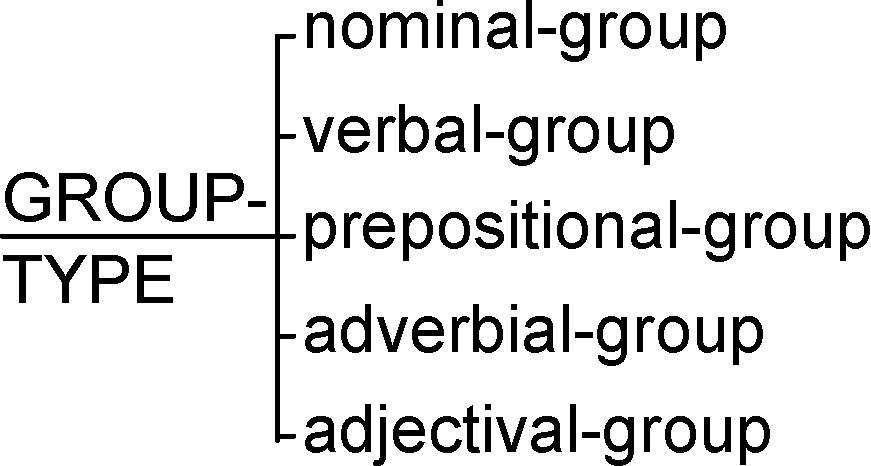
\includegraphics[width=0.57\linewidth]{Figures/SFL-grammar/group-classes.pdf}
		\caption{The group classes}
		\label{fig:group-classes-sub1}
	\end{subfigure}%
	\begin{subfigure}{.5\textwidth}
		\centering
		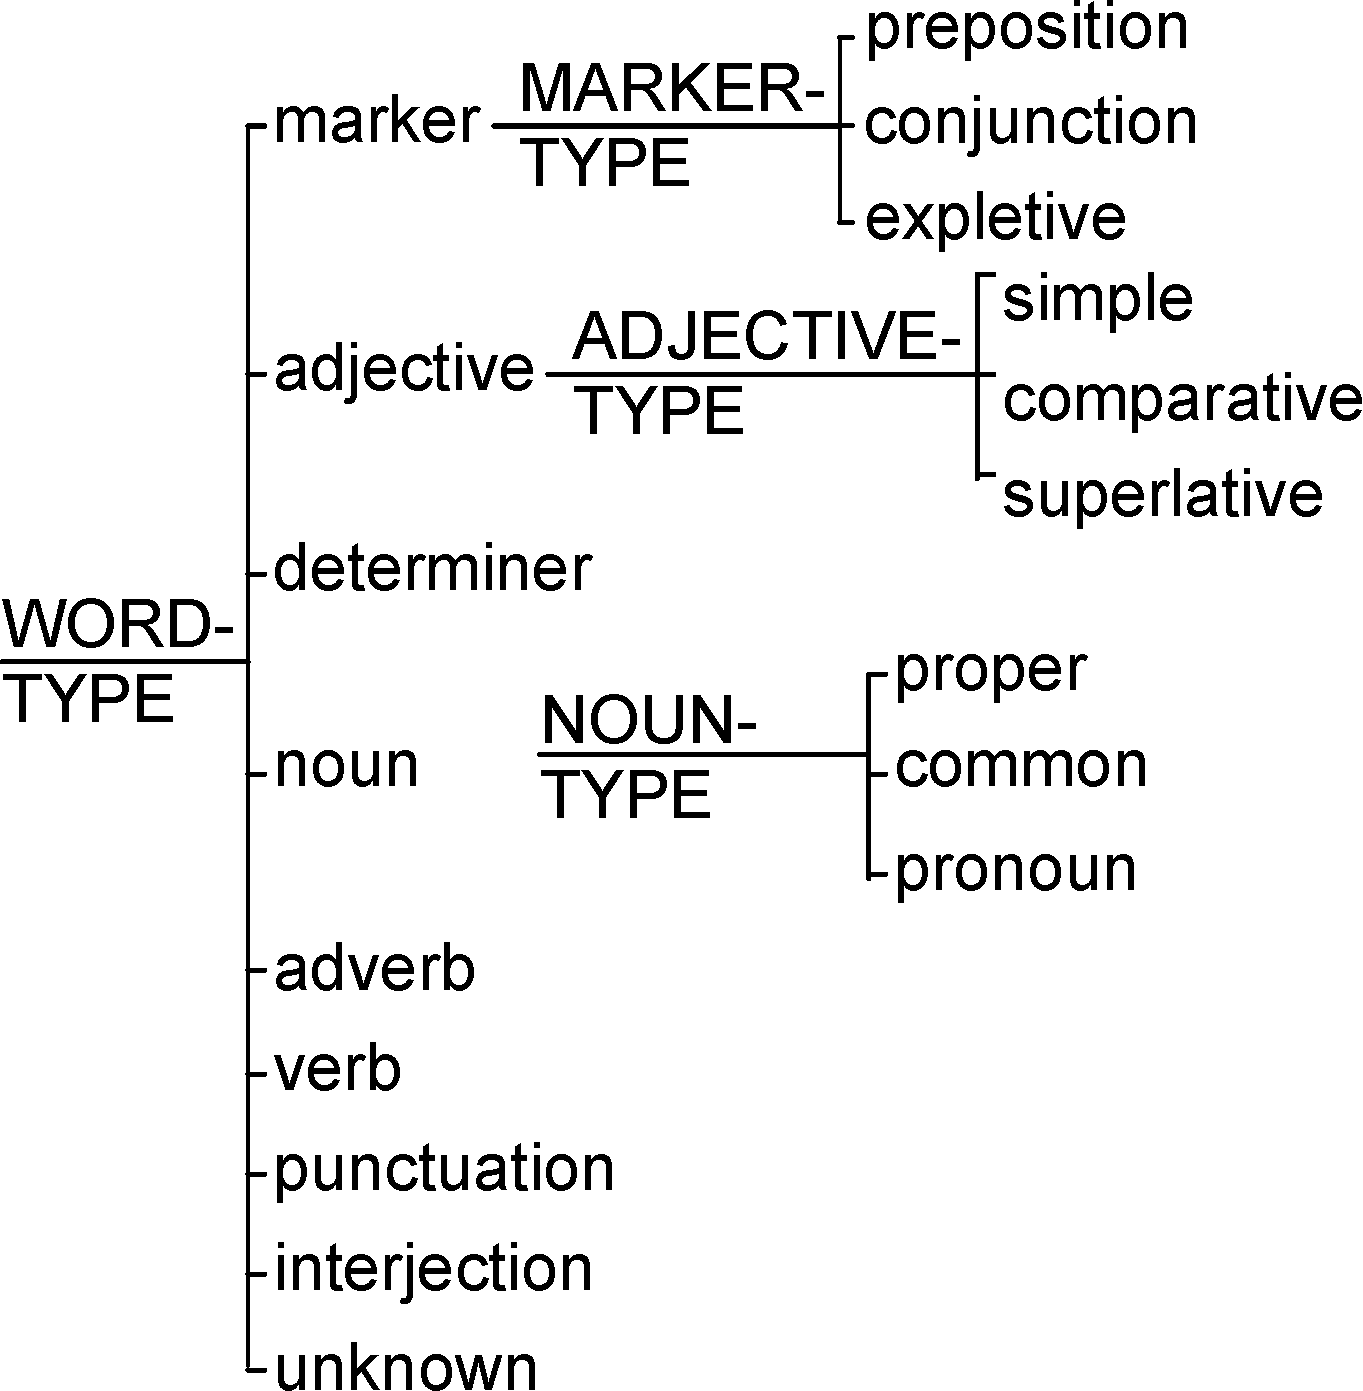
\includegraphics[width=0.9\linewidth]{Figures/SFL-grammar/word-classes.pdf}
		\caption{The word classes}
		\label{fig:group-classes-sub2}
	\end{subfigure}
	\caption{The group and word classes}
	\label{fig:group-classes}
\end{figure}

%The main reason is that Cardiff classes are beyond the syntactic variations of the grammar and blend into lexical semantics which makes it difficult to apply to parsing, at least nowadays with current state of word classification.

The word classes or part of speech tags that I adopt here are the ones employed to annotate Penn Treebank corpora called the Penn tag set \citep{Marcus1993} which, like Sidney unit classes, are also in line with the traditional grammar. This tag set has become a widely accepted standard in mainstream computational linguistics and there are multiple implementation of the part of speech taggers. The Stanford Parser which plays an important role in the software implementation of this thesis and is described in the Chapter \ref{ch:dependecy-grappamr}, employs precisely the Penn tag set.

The Penn tag set was developed to annotate the Penn Treebank corpora \citep{Marcus1993}. It is a large, richly articulated tag set that provides distinct codings for classes of words that have distinct grammatical behaviour.

The Penn tag set is based on the Brown Corpus tag set \citep{Kucera1968} but differs in several ways. First, the authors reduced the lexical and syntactic redundancy. In the Brown corpus there are many unique tags to a lexical item. In the Penn tag set the intention is to reduce this phenomenon to a minimum. Also distinctions that are recoverable from lexical variation of the same word such as verb or adjective forms or distinctions recoverable from syntactic structure are reduced to a single tag. 

Second the Penn Corpus takes into consideration the syntactic context. Thus the Penn tags, to a degree, encodes syntactic functions when possible. For example, \textit{one} is tagged as NN (singular common noun) when it is the head of the noun phrases rather than CD (cardinal number). 

Third, Penn POS set allows multiple tags per word, meaning that the annotators may be unsure of which one to choose in certain cases. There are 36 main POS and 12 other tags in the Penn tag set. A detailed description of the schema, the design principles and annotation guidelines are described in \citep{Santorini1990}. Figure \ref{fig:group-classes} depicts a classification summarising the Penn tag set. 

\subsection{The structure}
The \textit{unit} and \textit{structure} are two out of the four fundamental categories in the systemic theories of grammar. Sydney and Cardiff theories vary in their perspectives on \textit{unit} and \textit{structure} influencing how units are defined and identified.

For Halliday, the \textit{structure} (Definition \ref{def:structure}) characterises each unit as a carrier of a pattern of a particular order of \textit{elements}. The order is not necessarily linear realisation sequence but a theoretical relation of relative or absolute placement. This perspective has been proved useful in generation exercises where unit placement evolves in the realisation process.

The Cardiff School take a bottom up approach and defines class in terms of its internal structure describing a relative or absolute order of elements. This sort of syntagmatic account is precisely what is deemed useful in parsing and is the one adopted in this thesis. It is well established algorithmically how to recognise classes and construct them bottom up. So in our case easier to let the unit class emerge from recognition of constituent part-of-speech (word classes) and dependency relations between words or sequence of lower unit classes. In other words the unit class is defined by the unit structure and not by it's function in the parent unit, as Sydney school predicates, and this is precisely the reason why creation of constituency structure is computationally accessible. 


\subsection{Syntactic and semantic Heads}
%TODO: should this discussion of semantic and syntactic heads be here?
%TODO: provide Hallidayan analysis, my analisys and Cardiff analysis
%\todo{Should this discussion of semantic and syntactic heads be moved somewhere else?}
In SFG the heads may be semantic or syntactic. In most cases they coincide but there are exceptions when they differ or even miss. This is especially an important topic in the discussions of the nominal group structure on which \citet{Halliday2013} offer a thorough examination but \citet{Fawcett2000} offers us a more generic perspective on this issue.

Consider the example of nominal group ``a cup of tea'' analysed in three different ways in the Table \ref{tab:the-head-differences}. The Sydney Grammar offers two analyses in which the semantic and the syntactic heads differ. In the \textit{experiential} analysis the head is ``tea'' which functions as \textit{Thing}, while in the \textit{interpersonal} analysis the head is ``cup'' which functions as \textit{Head}. 

Cardiff Grammar does not make the Head/Thing distinction because the functional elements are already established based on semantic criteria.  discussed in subsection \ref{sec:nominal-group}. Nevertheless the logical analysis of SG resonates closely with the traditional ``semantically blinded'' grammars because it always provides a syntactic Head even if differs from the ``pivotal element'' of the group.

\begin{table}[h]
	\centering
	\begin{tabular}{|c|c|c|c|c|c|}
		\hline
		\multicolumn{2}{|c|}{} & \textbf{a} & \textbf{cup} & \textbf{of} & \textbf{tea} \\ \hline
		\multirow{2}{*}{Sidney Grammar} & experiential & \multicolumn{3}{c|}{\textit{Numerative}} & \textit{Thing} \\ \cline{2-6} 
		& interpersonal & \textit{Modifier} & \textit{Head} & \multicolumn{2}{c|}{\textit{Qualifier}} \\ \hline
		\multicolumn{2}{|l|}{Cardiff Grammar} & \multicolumn{2}{c|}{\textit{Quantifying Determiner}} & \textit{Selector} & \textit{Head} \\ \hline
	\end{tabular}
	\caption{Example of dispersed semantic and syntactic heads}
	\label{tab:the-head-differences}
\end{table}

Fawcett argues that none of the constituting elements of the unit is mandatory realised even the so called \textit{``pivotal element''} which is the group defining element. The logical structure heads are always realised and correspond dependency relations established in the DG. Depending on the unit class logical structure heads are conflated with specific functions, for instance in nominal group the Head is usually conflated with the Thing, in quality group with the Apex, in quantity group with the Amount, in clause with the Main Verb and so on. But in language it is not unusual to have nominal groups with the Thing missing or elliptic clauses with missing the Main verb so no rigid correspondence can be established between the Head, unit class and the corresponding pivotal element of the group. So because the unit class depends on its internal structure leading to a circular interdependency between the unit class and the unit structure. To solve this issue Fawcett argues for bototm-up approach where head-modifier relations are identified between lexical items and then between units (i.e. groups and clauses) serving as cues to identify elements of the higher unit and therefore it's class. Usually the class membership of head is raised to the unit class although sometimes the presence or absence of certain elements (during the reconstruction process) may alter the unit class to a different from the logical head. 

\begin{exe}
	\ex\label{ex:the-old-example} The old shall pass first.
\end{exe}

Consider the nominal group ``The old'' which is the subject in example \ref{ex:the-old-example}. The head of the nominal group is the adjective ``old'' and not a noun as it would normally be expected. The noun modified by the adjective ``old'' is left covert and it shall be recoverable from the context. We can insert a generic noun ``one'' to form a canonical noun group:``the old one''. In such cases when the head noun is missing, the logical head is conflated with other element in this case the Epithet. The group class is not raised from the word class to quality group but is identified by internal structure  of the whole group and in this case the presence of determiner signals a nominal class. I point out through this example that the class of the head is not always is raised to establish the group class but the whole underlying structure determines the group class.

\subsection{Systems and systemic networks}
%\label{sec:system}
% exemplification of system
%TODO: Margaret Berry on Systems/Networks, David Butt on Systems, see citations in Rebekas's Thesis
%TODO: write email to Rebekah and ask about theory comparison literature

Fore example consider polarity system represented in figure \ref{fig:polarity}. It contains two choices either positive or negative. And when one says it is positive one means not negative which is obvious and self evident how the two choices are mutually exclusive.

\begin{figure}[H]
	\centering
	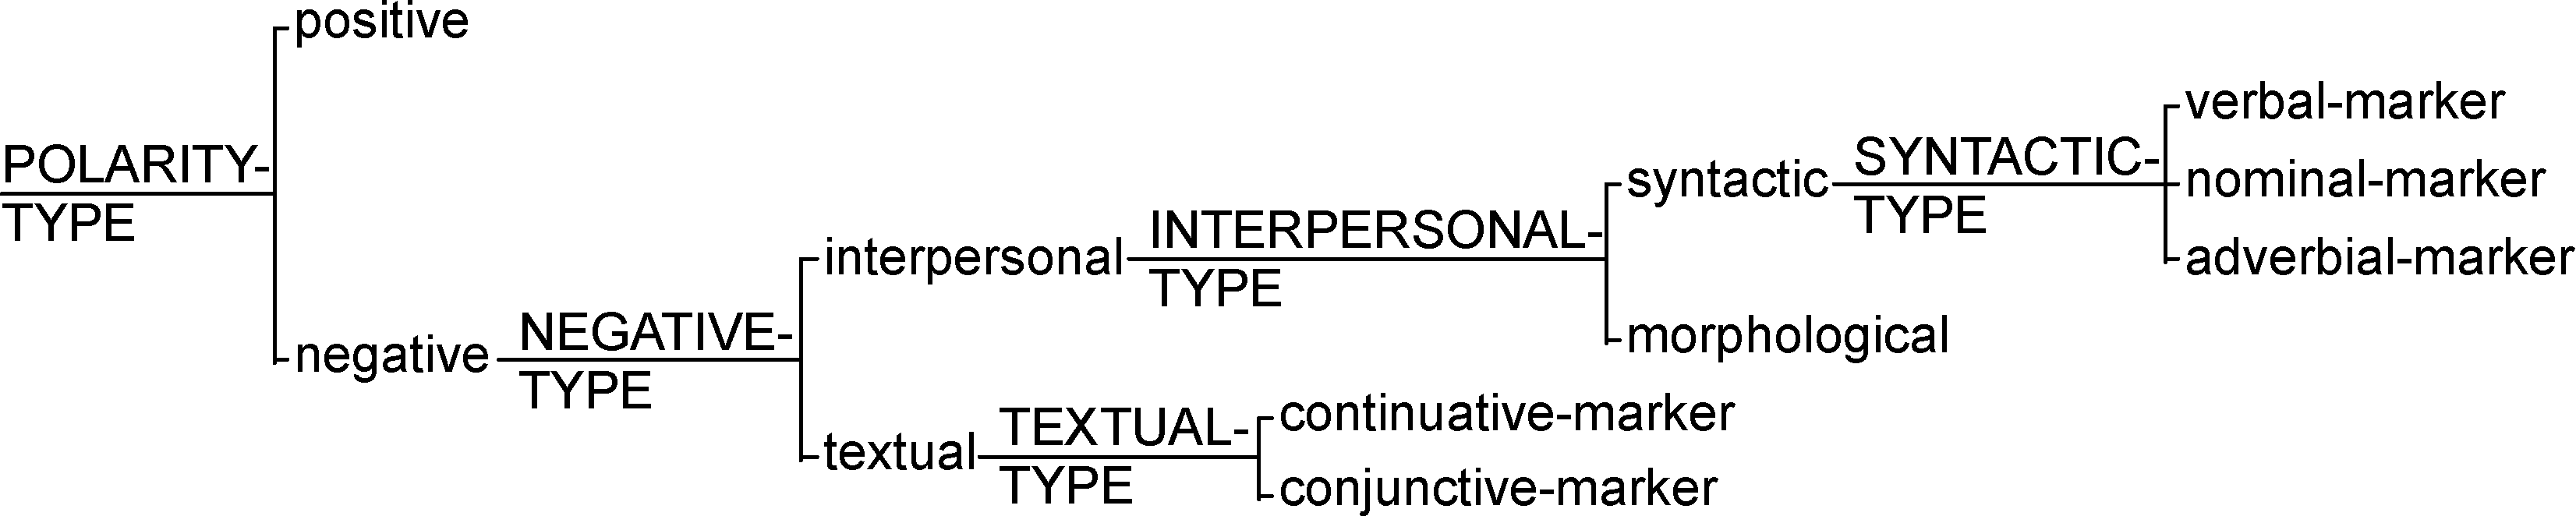
\includegraphics[width=\textwidth]{Figures/SFL-grammar/polarity-system.pdf}
	\caption{System network of POLARITY}
	\label{fig:polarity}
\end{figure}

In language it may be often the case that a choice in a system may lead to re-entering the same system again to make another choice again forming this way recursive systems. Alternatively, we can say that a system allows multiple choices for the same unit. These perspectives are the sides of the same coin where the recursion perspective is useful for natural language generation while multiple choice perspective suits better the parsing task and next I explain why by continuing the discussion on polarity system. 

The negative polarity in English clauses can be realised in several ways: via a noun group with intrinsic negative polarity feature like \textit{``nobody''} (\ref{ex:neg1}), negation particle of the verb \textit{``n't''} (\ref{ex:neg2}) or adverb with intrinsic negative polarity (\ref{ex:neg3}). 

\begin{exe}
	\ex\label{ex:neg1} Nobody with any sense is going. 
	\ex\label{ex:neg2} I don't have to mow my lawn.
	\ex\label{ex:neg3} Never expect her to come back.
\end{exe}

Consider now, the cases of double negation from the example \ref{ex:double-negatives1} where two kinds of negations are realised in the same clause: the negation by verb particle \textit{``n't''} and the pronoun \textit{``nobody''}. 

\begin{exe}
	\ex \label{ex:double-negatives1}
	Nobody with any sense isn't going. 
	\ex \label{ex:double-negatives2} I don’t have nobody to mow my lawn.
\end{exe}

The systems can be recursive and thus choices are not always mutually exclusive. Even though the system network  clearly distinguishes one type of negation from another multiple negations can still occurring simultaneously. Note that this more delicate distinctions in kind of negation, still is a negation and for any of them it is impossible to co-occur with positive polarity. 
The issue here is not semantic about whether the clause is positive or negative but what kinds of grammatical choices can be identified within the clause. The problem of whether the double negation shall be interpreted as positive is not necessarily as relevant as the task of identifying the two instances of negation. 

Halliday states that the speaker makes only one choice from a system. If this rule is interpreted as two choices from the same system at a time being impossible then it clearly does not cover the recursive systems and needs weakening to accommodate border cases. I propose relaxing the constraint of \textit{mutual exclusivity} to \textit{disjunction}. Correspondingly, two types of systemic networks emerge differing by \textit{the relation among choices}: the original Hallidayan XOR systems (such as POLARITY TYPE in figure \ref{fig:polarity}) and the OR systems for accommodating cases of multiple feature selections (such as SYSTEMIC TYPE in the same figure).

% entry condition relationship types
As system is expanded in delicacy to forms a systemic network of choices. Choice of a feature in one system becomes the entry condition for choices in more delicate systems below. I turn now to discuss the relationship types of relationships forming entry conditions to more delicate systems. For instance, an increase in delicacy can be seen as a taxonomic ``is a'' relationship between features of higher systems and lower systems like in the case of POLARITY TYPE and NEGATIVE TYPE in figure \ref{fig:polarity}. 

\begin{figure}[hbtp]
	\centering
	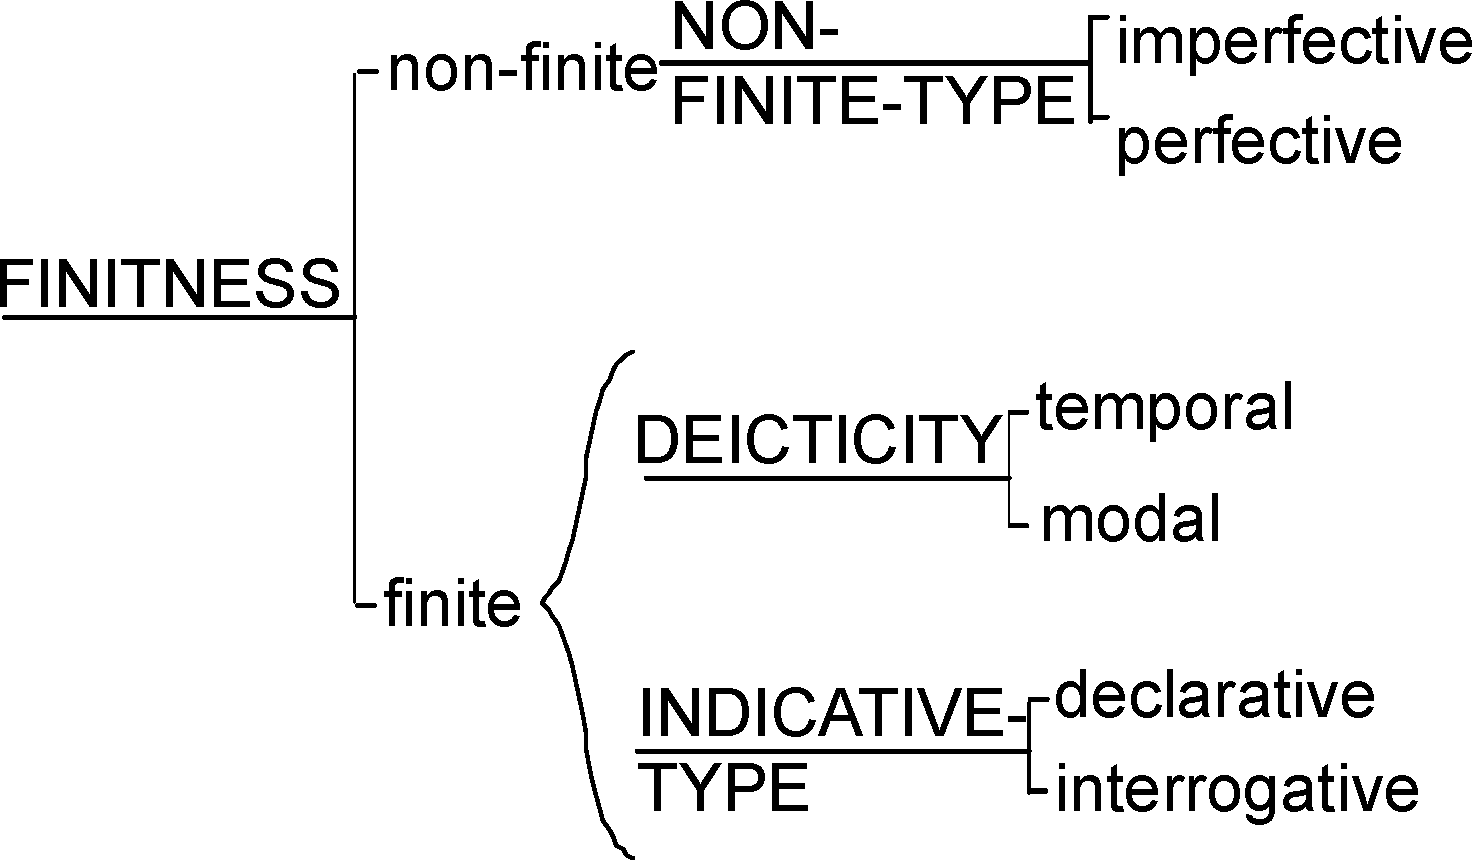
\includegraphics[width=0.5\textwidth]{Figures/SFL-grammar/finitness-system.pdf}
	\caption{A fraction of the finiteness system where increase of delicacy is not ``is a'' relation}
	\label{fig:finitness-fraction}
\end{figure}

The activation relation among systems in the cline of delicacy is not always taxonomic. Another relation is ``enables selection of'' without a any sub-categorisation implied. For example see FINITENESS system in figure \ref{fig:finitness-fraction} where in case that the finite option is selected then what this choice enables are not subtypes of finite but merely other options that become available i.e. DEIXIS and INDICATIVE TYPE. The latter is there because selection of finite implies also selection of indicative feature in a FINITNES's sibling system MOOD-TYPE comprised of options indicative vs. imperative. 

In this subsection I defined the system and systemic network, presented two system types by the relationship between their choices and distinguished two kinds of activation relations between systems on the cline of delicacy.

\subsection{coordination as unit complexing}
%TODO: the complex class is semantic and not grammatical
%TODO: sometimes the second element is more representative of the complex or the first one maybe, maybe just take the class of the first unit and then ingnore teh class of the rest, or the last one and ingnore classes of the first ones

\label{sec:coordination}
In SG unit complexes fill an important part of the grammar along with the \textit{taxis relations} which express the interdependency relations in unit complexes. \textit{Parataxis} relations bind units of equal status while the \textit{Hypotaxis} ones bind the dominant and  the dependant units. Fawcett bypasses the taxis relations replacing them with coordination and embedding \citep[271]{Fawcett2000} seemingly an oversimplified approach leading to abandonment of unit complexing as well. While embedding accounts for the depth and complexity of syntax his approach to coordination is problematic. I further discuss and argue for utility of unit-complexes for the coordination but this idea can be further extended to other phenomena which involve fixed idiomatic structures such as comparatives or conditionals.

Coordination is challenge not only for SFL but for other linguistic theories as well. CG treats this phenomena as two or more units filling or expounding the same element. For example, in table \ref{ex:Cardiff-example-analisys} ``his shirt'' and ``and his jeans'' are two nominal groups that are siblings and both of them fill the same complement. 

\begin{table}[h]
	\centering
	\begin{tabular}{|c|c|c|c|c|c|c|}
		\hline
		\textit{Ike} & \textit{washed} & \textit{his} & \textit{shirt} & \textit{and} & \textit{his} & \textit{jeans} \\ \hline
		Subject         & Main Verb               & \multicolumn{5}{c|}{Complement}                                                    \\ \hline
		&                 & \multicolumn{2}{c|}{Nominal Group}      & \multicolumn{3}{c|}{Nominal Group}                     \\ \hline
		&                 & Deictic Determiner           & Head              & \&           & Deictic Determiner           & Head              \\ \hline
	\end{tabular}
	\caption{Coordination analysis in Cardiff Grammar}
	\label{ex:Cardiff-example-analisys}
\end{table}

In SG the coordination is analised as a \textit{complex unit} held together through paratactic relations ensuring that only one unit fills an element of the parent constituent in our example the complement of the clause. The table \ref{ex:Sydeny-example-analisys} illustrates an example analysis involving the complex unit approach. 

\begin{table}[h]
	\centering
	\begin{tabular}{|c|c|c|c|c|c|c|}
		\hline
		\textit{Ike}     & \textit{washed}      & \textit{his} & \textit{shirt} & \textit{and} & \textit{his} & \textit{jeans} \\ \hline
		Subject          & Predicate/Finite     & \multicolumn{5}{c|}{Complement}                                              \\ \hline
		\multicolumn{2}{|c|}{\multirow{3}{*}{}} & \multicolumn{5}{c|}{nominal group complex}                                   \\ \cline{3-7} 
		\multicolumn{2}{|c|}{}                  & \multicolumn{2}{c|}{1}        & \multicolumn{3}{c|}{+2}                      \\ \cline{3-7} 
		\multicolumn{2}{|c|}{}                  & Deictic      & Thing          & \&           & Deictic      & Thing          \\ \hline
	\end{tabular}
	\caption{Coordination analysis in Sydney Grammar}
	\label{ex:Sydeny-example-analisys}
\end{table}

The opinions are divided by whether to invite the notion of a complex unit to handle coordination or not. If we dismiss the unit complex then an element could be filled by more than one units and if we adopt it then the complexing relations need to be accounted along with unit class and what is its structure.

I would argue for adoption of such unit type for two reasons. First, only units are accounted for structure while the elements can only be filled by an unit. Allowing multiple units to fill an element requires accounting at least for order if not also for the relation between the units. The structure as it is described in theories of grammar by Halliday \citep{Halliday2002} and Fawcett \citep{Fawcett2000} is defined in the unit and not the element. A unit has a specific possible structure in terms of places of elements however if an element is filled by two units simultaneously it constitutes a violation of the above principle as the order of those units is not accounted for but it matters.
\begin{exe}
	\ex\label{ex:conj2-extra-marker1}
	(Both my wife and her friend) arrived late.  
	\ex\label{ex:conj2-extra-marker11} * (And her friend both my wife) arrived late.
	\ex\label{ex:conj2-extra-marker2}
	I want the front wall (either in blue or in green). 
	\ex\label{ex:conj2-extra-marker21}
	* I want the front wall (or in green either in blue). 
\end{exe}

If the order would not have mattered then we could say that the conjunctions from the example \ref{ex:conj2-extra-marker1} can be reformulated into \ref{ex:conj2-extra-marker11} and the one from \ref{ex:conj2-extra-marker2} into \ref{ex:conj2-extra-marker21}. But such reformulations are grammatically incorrect. Obviously the places do matter and they need to be described in the unit structure. 

Secondly, the lexical items that signal the conjunction are not a part of the conjuncted units. This is contrary to what is being described in Cardiff and Sydney grammars. Fawcett present the Linker elements (\&) which are filled by conjunctions as parts of virtually any unit class placed in the first position of the unit. Halliday omits to discuss in IFG \citep{Halliday2013} the place of Linkers but implicitly proposes the same as Fawcett through his examples of paratactic relations at various rank levels where the lexical items signalling conjunction are included in the units they precede.

For example in the ``or in green'' the presence of ``or'' signalls the presence at least of one more unit of the same nature and does not contribute to the meaning of the prepositional group but to the meaning outside the group requiring presence of a sibling. Even more, the lack of a sibling most of the time would constitute an ungrammatical formulation. I say sometimes because it is perfectly acceptable to start a clause/sentence with a conjunction most often ``but''. But even in those cases it still invites the presence of a sibling clause/sentence preceding the current one to be resolved at the discourse level. 

So conjunctions and pre-conjunctions shall not be placed as elements of the conjuncted units because they do not contribute to their meaning.

Adopting the unit complex and in particular coordination unit requires two clarifications (1) does the unit complex carry a syntactic class, and if so according to which criteria is it established? (2) Does it have any intrinsic features or not?

Zhang states in her thesis that the coordinating constructions do not have any categorial features thus there is no need to provide a new unit type. Instead the categorial properties of the conjuncts are transferred upwards \citep{NinaZhang2010}. For example if two nominal groups are conjuncted then the complex receives the nominal class. This principle holds for most of the cases however there are rare cases when the units are of different classes. Consider the example \ref{ex:conj3-different-unit-types} where the conjuncts are a nominal group ``last Monday'' and a prepositional group ``during the previous weekend''.
\begin{exe}
	\ex\label{ex:conj3-different-unit-types}
	I lost it (either last Monday or during the previous weekend). 
\end{exe}

%In unit types are of different classes: a nominal group and a prepositional phrase.
In this case there are two unit types that can be raised and it is not clear how to resolve this case. Options are to leave the class unspecified, transfer the class of the first unit upwards, or semantically resolve the class as both represent temporal circumstances even if they are realised through two different syntactic categories. Another option is to leave the class generic and assign the conjunction unit the class of \textit{``coordination complex''} without sub-classifying it according to the constituent units below, i.e. without upward unit class transfer. 

I address the second question regarding the intrinsic features of the complex unit. The coordination complex can have categorial features which none of the constituting units has. In the example \ref{ex:conj-plural-right} the conjunction of two singular noun groups requires plural agreement with the verb. Even though semantic interpretation that only one item is selected at a time, syntactically both items are listed in the clause and attempting third person singular verb forms like in \ref{ex:conj-plural-wrong} is grammatically incorrect.
\begin{exe}
	\ex\label{ex:conj-plural-right}
	A pencil or a pen \textbf{are} equally good as a smart-phone.
	%\ex\label{ex:conj-plural-right1} A fork and knife \textit{have} to be placed on the sides of each plate.
	\ex\label{ex:conj-plural-wrong} * A pencil or a pen \textbf{is} equally good as a smart-phone.
	%\ex\label{ex:conj-plural-wrong1} * A fork and knife \textit{has} to be placed on the sides of each plate.
\end{exe}
\begin{figure}[hbtp]
	\centering
	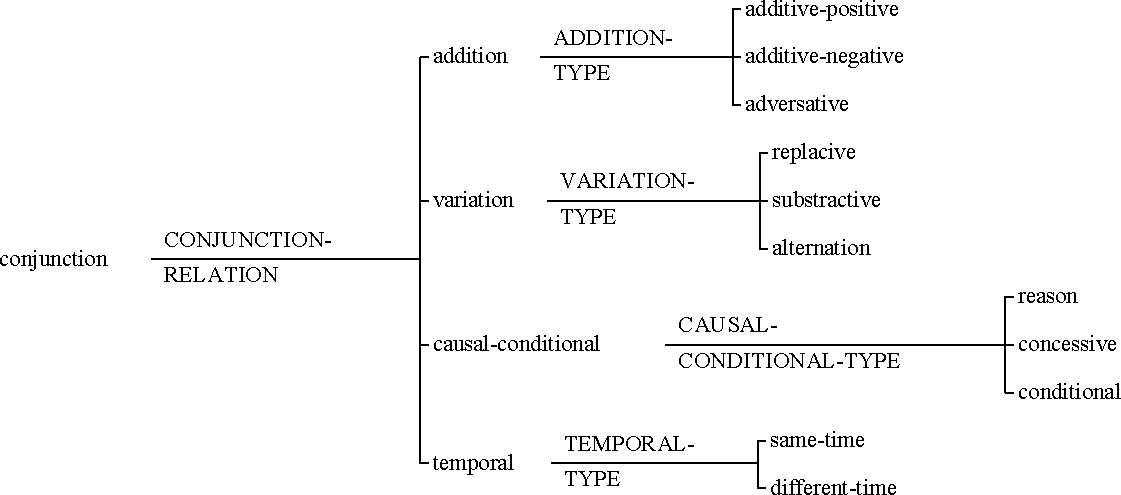
\includegraphics[width=\textwidth]{Figures/SFL-grammar/conjunction-system.pdf}
	\caption{Systemic network of coordination types}
	\label{fig:conj-rel-types}
\end{figure}

In the case of nominal group conjunction we can see that the plural feature emerges even if each individual unit is singular. For other unit classes it is not so obvious whether there are any linguistic features that emerge to the conjunction level. The meaning variation is rather semantic as for example conjunction of two verbs or clauses might mean very different things like consecutive actions, concomitant actions or presence of two states at the same time and so on. This brings us to another feature of the coordination complex - the type of the relationship it constructs. The lexical choice of head conjunct is the indicator of relationship among the conjuncts. Either \textit{and}, \textit{or}, \textit{but}, \textit{yet}, \textit{for}, \textit{nor} or \textit{so} they express different meanings which are well representable as a  relationship types systemic network in figure \ref{fig:conj-rel-types}.


%The coordination complex has a structure as depicted in figure \ref{fig:coord-complex-elements}. The lexical item signalling the coordination complex is the head of the construction. The Conjunct elements are the ones being related to each other and they can be filled or expounded by virtually any unit type. The Enumerator element substitutes the head and delimits the Conjuncts when there are more than two of them. The Enumerator is almost always a comma in written texts. 

Adopting the unit complexing enables various kinds of constructions and coordination is only one of them. Below we discuss taxis relations and their role in unit complexing.

\section{Critical discussion of the grammatical units}
\label{sec:discussion-unit-classes}

Now that the important theoretical details have been covered I would like focus on the grammars of the two schools. They have common parts and also differ in large parts on their paradigmatic and syntagmatic descriptions. This section discusses the main units considered in each of the grammars. Like in the previous section I argue on pragmatic grounds for adoption of unit structures from either grammar. This may seem like an inconsistency add below I try to convince you of the opposite below. The argument runs along the line that some unit structures are closer to the syntactic analysis and thus are easier to detect and parse and the other ones may be a level of abstraction higher falling more on the semantic grounds thus becoming more difficult to capture in structural variance and requiring lexico-semantic resources.

For the reasons of limited space I skipped introducing the Sydney and Cardiff grammars and in turn assume that the reader is familiar with the details fo both of them. And for a general overview of the unit structure in each of the grammars please refer to Appendix \ref{ch:syntax-overview}. Nevertheless, as it is a parallel contrastive discussion, even if the reader is familiar with one grammar only I hope it becomes clear how does certain phenomena are dealt with in the other one. 

\subsection{The verbal group and clause division}
\label{sec:verbal-grpoup-and-clause-division}
In SG the verbal group is described as an expansion of a verb just like the nominal group is the expansion of the noun\citep[396]{Halliday2013}. There are certainly words that are closely related and syntactically dependent on the verb all together forming a unit that functions as a whole. For example the auxiliary verbs, adverbs or the negation particles are words that are directly linked to a lexical verb. The verb group functions as Finite + Predicator elements of the clause in mood structure and as Process in Transitivity structure. 

In CG the verb group is dissolved moving the Main Verb as the pivotal element of the Clause unit. All the elements that form the clause structure and those that form the verb group structure are brought up together to the same level as elements of a clause. The clause structure in CG comprises elements with clause related functions(like Subject, Adjunct, Complement etc.) and other elements with Main Verb related functions(Auxiliary, Negation particle, Finite operator etc.).

Regarding from the Hallidayan rank scale perspective, merging the elements of the verb group into clause structure is not permitted because the units are of different rank scales. However it is not a problem for the relaxed rank scale version presented in subsection \ref{sec:rank-system}. The reason for adopting such an approach is best illustrated via complex verb groups with more than one non-auxiliary verb such as in examples \ref{ex:complex-verb-groups1}--\ref{ex:complex-verb-groups3}. 

Next I address the impact of this merger on (a) the clause structure (b) the clause boundaries and (c) semantic role distribution within the clause.

\begin{exe}
	\ex\label{ex:complex-verb-groups1}
	(The commission \textbf{started to investigate} two cases of overfishing in Norway.)  
	\ex\label{ex:complex-verb-groups2}
	(The commission \textbf{started} (\textbf{to investigate} two cases of overfishing in Norway.))
	\ex\label{ex:complex-verb-groups3}
	(The commission \textbf{started} (\textbf{to finish} (\textbf{investigating} two cases of overfishing in Norway.)))
\end{exe}

%Then answers to the above questions boil down to whether we allow for more than one lexical verb per predicate or not. 
In SG ``started to investigate'' (example \ref{ex:complex-verb-groups1}) is considered a single predicate of investigation which has specified the aspect of event incipiency despite the fact that there are two lexical verbs within the same verbal group. The ``starting'' doesn't constitute any kind of process in semantic terms but rather specifies aspectual information about the investigation process. The boundaries of the clause governed by this predicate stretch to entire sentence.

Semantically it is a sound approach because despite the presence of two lexical verbs there is only one event. However allowing such compositions leads to unwanted syntactic analysis for multiple lexical verb cases like in example \ref{ex:complex-verb-groups3}.To solve this kind of problems Fawcett dismisses the verb groups and merges their elements into clause structure. He proposes the syntactically elegant principle of \textit{``one main verb per clause''} \citep{Fawcett2008}. Apply this principle to the same sentence yields a structure of two clauses illustrated in example \ref{ex:complex-verb-groups2} where the main clause is governed by the verb ``to start'' and the embedded one by the verb ``to investigate''. Note the conflict between ``one main verb per clause'' with Halliday's principle that only whole units form the constituency of others (the (c) principle of rank scale described in subsection \ref{sec:rank-system}). So allowing incomplete groups into the constituency structure would breach entire idea of unit based constituency. 

Semantically the clause in SFL is a description of an event or situation as a figure with a process, participants and eventually circumstances where the process is realised through a lexical verb. Looking back to our examples, does the verb ``to start'' really describes a process or merely an aspect of it? Halliday treats such verbs as aspectual and when co-occurring with other lexical verbs are considered to form a single predicate. Accommodating Fawcett's stance, mentioned above and contradicting Halliday's approach, requires weakening the semantic requirement and allowing aspectual verbs to form clauses that contribute \textit{aspectually or modally} to the embedded ones. I mention also the modal contribution because some verbs like \textit{want, wish, hope}, etc. behave syntactically exactly like the aspectual ones. Moreover, Fawcett introduces into CG Transitivity network ``influential'' process type including all categories of meanings that semantically function as process modifiers: tentative, failing, starting, ending etc.

Fawcett's ``one main verb per clause'' principle changes the way clauses are partitioned, leads to abolition of the verbal group and introduces the ``influential'' process type.

\subsection{The Clause}
\label{sec:cardiff-clause}
It is commonly agreed in linguistic communities that the unit of clause is one of the core elements in human language. It is consider the syntactic unit that expresses semantic units of a situation referring to a potentially rich array of meanings. The clause structure has been studied for long time and the main clause constituents are roughly the same in SFL as the ones in the traditional grammar \citep{Quirk1985}, transformational grammar \citep{Chomsky1957} an indirectly in dependency grammar \citep{Hudson2010}.

In current work I adopt the CG Clause structure with the \textit{Main Verb} as pivotal element. Though there is no element that is obligatorily realised in English language, the Main Verb is realised with a reliably high degree of probability. Exceptions are the minor clauses (exclamations, calls, greetings and alarms) that occur in conversational contexts and elliptical clauses \citet{Halliday2013} such as the one in example \ref{ex:elipted-clause} which are not currently covered.

\begin{exe}
	\ex\label{ex:elipted-clause} They were in the bar, \textit{Dave in the restroom and Sarah by the bar}.
\end{exe}

As mentioned before \ref{structure} the elements of a structure are defined in terms of their function contributing to the formation of the whole unit. The elements of an English clause are \textit{Subject}, \textit{Finite}, \textit{Main Verb}(a part of the Predicator), up to two \textit{Complements} and a various number of \textit{Adjuncts}. All the elements of the assumed verbal group are part of the clause as well such as Auxiliary Verbs, Main Verb Extensions, Negators etc. (see Appendix \ref{ch:syntax-overview} for a complete list). 

%\todo*{}{TODO continue, maybe mention about the clause complexing}
%SFG accounts for how clauses form nexuses of tactic relations (see Definition \ref{def:taxis}).


\subsection{The Nominal Group}
\label{sec:nominal-group}
The nominal group expresses things, classes of things or a selection of instances in that class. In the table \ref{tab:example-ng} is presented an example analysis of the nominal group proposed in Sydney grammar \citep[364--369]{Halliday2013}. 
\begin{table}[!ht]
	\begin{tabular}{|c|c|c|c|c|c|}
		\hline
		\textit{those} & \textit{two} & \textit{old} & \textit{electric} & \textit{trains} & \textit{from Luxembourg} \\ \hline
		\multicolumn{4}{|c|}{pre-modifier}                               & head            & post-modifier            \\ \hline
		Deictic        & Numerative   & Epithet      & Classifier        & Thing           & Qualifyier               \\ \hline
		determiner     & numeral      & adjective    & adjective         & noun            & prepositional phrase     \\ \hline
	\end{tabular}
	\caption{The example of a nominal group in Sydeny Grammar}
	\label{tab:example-ng}
\end{table}

In SG it is constituted by a head nominal item modified by descriptors or selectors such as: \textit{Deictic}, \textit{Numerative}, \textit{Epithet}, \textit{Classifier}, \textit{Thing} and \textit{Qualifier}. Each element has a fairly stable correspondence to the word classes, expected to be expounded by lexical items. The table \ref{tab:function-pos-mapping} presents the mappings between the functions and the word classes.

\begin{table}[h]
	\begin{tabular}{|c|c|}
		\hline
		\textbf{Experiential function in noun group} & \textbf{class (of word or unit)} \\ \hline
		Deictic                             & determiner, predeterminer, pronoun \\ \hline
		Epithet                             & adjective                    \\ \hline
		Numerative                          & numeral(ordinal,cardinal)    \\ \hline
		Classifier                          & adjective, noun              \\ \hline
		Thing                               & noun                         \\ \hline
		Qualifier                           & prepositional phrase, clause \\ \hline
	\end{tabular}
	\caption{The mapping of noun group elements to classes}
	\label{tab:function-pos-mapping}
\end{table}

%There is little variation in how these functions are linked to the word classes. However the variation is not provided in the Sydney Grammar as it is in Cardiff Grammar. The latter provides data driven filling probabilities for each functional element to a set of possible unit classes \citep{Fawcett2000}.

The elements in CG differ from those of SG. The table \ref{tab:carfiff-ng} exemplifies a noun group analysed with CG covering all the possible elements. The table \ref{tab:cg-mappings} provides a legend for CG acronyms along with mappings to unit and word classes that can fill each element.

\begin{table}[H]
	\resizebox{\linewidth}{!}{
		\begin{tabular}{|c|c|c|c|c|c|c|c|c|c|c|c|c|c|c|}
			\hline
			\textit{or} & \textit{a photo} & \textit{of} & \textit{part} & \textit{of} & \textit{one} & \textit{of} & \textit{the best} & \textit{of} & \textit{the} & \textit{fine} & \textit{new} & \textit{taxis} & \textit{in Kew} & \textit{,} \\ \hline
			\multicolumn{12}{|c|}{pre-modifiers} & head & \multicolumn{2}{c|}{post-modifiers} \\ \hline
			\& & rd & v & pd & v & qd & v & sd or od & v & dd & m & m & h & q & e \\ \hline
		\end{tabular}}
		\caption{The example of a nominal group in Cardiff Grammar}
		\label{tab:carfiff-ng}
	\end{table}
	%
	\begin{table}[h]
		\begin{tabular}{|c|c|c|}
			\hline
			\textbf{symbol} & \textbf{function meaning} & \textbf{class (of word or unit)} \\ \hline
			rd & representational determiner & noun, noun group \\ \hline
			v & selector ``of'' & preposition \\ \hline
			pd & partitive determiner & noun, noun group \\ \hline
			fd & fractional determiner & noun, noun group, quantity group \\ \hline
			qd & quantifying determiner & noun, noun group, quantity group \\ \hline
			sd & superlative determiner & noun, noun group, quality group, quantity group \\ \hline
			od & ordinative determiner & noun, noun group, quality group \\ \hline
			td & tipic determiner & noun, noun group \\ \hline
			dd & deictic determiner & determiner, pronoun, genitive cluster \\ \hline
			m & modifier & adjective, noun, quality group, genitive cluster \\ \hline
			h & head & noun, genitive cluster \\ \hline
			q & qualifier & prepositional phrase, clause \\ \hline
			\& & linker & conjunction \\ \hline
			e & ender & punctuation mark \\ \hline
		\end{tabular}
		\caption{The mapping of noun group elements to classes in Cardiff grammar}
		\label{tab:cg-mappings}
	\end{table}
	%
	
	The elements in CG have are based on semantic criteria supported by lexical and syntactic choices. Consequently some elements cannot be derived based on solely syntactic criteria requiring semantically motivated lexical resources. Semantically bound elements are predominantly determiners \textit{Representational, Partitive, Fractional, Superlative, Typic Determiners} while the rest of the elements: \textit{Head, Qualifier, Selector, Modifier and Deictic, Ordinative and Quantifying Determiners} can be determined solely on the syntactic criteria. The latter correspond fairly well to Sydney version of nominal group which is adopted in present work with the  benefits of relaxed rank system replacing the sub-structures with embedded units and simplifying the syntactic structures. 
	
	%3. introduction of negation element, linker, punctuation
	%``No'' as determiner. negative pronoun noone.
	%\citep[62,109,185]{Quirk1985}, \citep[365--374]{Halliday2013}, 
	%
	%The negation element is in Cardiff Grammar in clause structure so that it is separated from the finite. It's adoption in noun structure might or might not be a good idea. It is useful for complex groups. 
	%
	%\begin{exe}
	%\ex \label{ex:example-of-no}
	%No breathing man or animal can escape that forest alive.
	%\end{exe} 
	
	Another simplification is renouncing to distinction between the Head and Thing \citep[390--396]{Halliday2013} for the semantic ambiguity reasons as the determiners in CG. Thus if the logical Head of the nominal group is a noun then it is labelled as the Thing leaving the semantic discernment as a secondary process and out of the current scope. Otherwise, in cases of nominal groups without the Thing element, if the Head is pronoun(other than personal), numeral or adjective (mainly superlatives) then they function as Deictic, Numerative or Epithet. So I propose to parse the nominal groups in two steps: first determine the main constituting chunks and assign functions to the unambiguous ones and second perform a semantically driven evaluation for the less certain units.
	
%	\todo*{probably remove: discussion of Head/Thing and CG determiners distinction}{
		In other cases the Thing is present but it is different from the Head. Consider example \ref{ex:dectic-ngs}. In Sydney grammar they're treated as a nominal groups with qualifiers introduced by the \textit{``of''} preposition. But these nominal groups are not really about the ``cup'', ``some'' or ``another one'' but rather about ``tea'', ``youngsters'' and ``eruptions''. 
		\begin{exe}
			\ex \label{ex:dectic-ngs} (a cup) of (tea)
			\ex (some) of (those youngsters)
			\ex (another one) of (those periodic eruptions)
		\end{exe}
		So then the syntactic Head still remains the first noun in the nominal group, but then by a semantic evaluation the Thing is shifted into the Qualifier introduced by ``of'' preposition. Cardiff Grammar weakens the assumption that every prepositional phrase acts as Qualifier in a nominal group and it the special case of the preposition ``of''. It is allowed to act not as the element introducing a prepositional phrase but as a end mark of a determiner-like selector. Thus making the former noun group a determiner in the latter one. This approach shifts the noun group head into the position of semantically based Thing and erases the discrepancy problem between them. Nonetheless this is not straight forward solution as it requires lexical-semantic informed decision.
        % However this is not straight forward solution. There is a lot of space for variations the syntactic structure. 
        For example in \ref{ex:of-qualifiers} (Head/Thing marked in bold) the preposition ``of'' introduces Qualifiers. 
		\begin{exe}
			\ex \label{ex:of-qualifiers}
			He was the \textbf{confidant} of the prime minister.
			\ex It was the \textbf{clash} of two cultures.
		\end{exe}
		
		The distinction between cases when the proposition ``of'' introduces a Qualifier or ends a Selector/Deictic requires a semantic evaluation answering the questions ``what is the Thing that this nominal group is about?''. While it is easy to just assume that the first noun in the nominal group is the head. 
        
        Therefore, I propose to parse the nominal groups in two steps: first determine the main constituting chunks and assign functions to the unambiguous ones and then in the second step to perform a semantically driven evaluation for the less certain units. This evaluation can be performed by further capturing the structure of nominal groups that act as Dyslectics through their lexico-syntactic realisation patterns.
%	}
	
	\subsection{The Adjectival and Adverbial Groups}
	\label{sec:advectival-adverbial-groups}
%	\todo{Revise the whole subsection}
	Following the rationale of head-modifier like in the case of nominal groups, the adjectives and adverbs function as pivotal elements to form groups. The structure of adverbial and adjectival constructions is briefly covered in Sydney grammar in terms of head-modifier logical structures without an elaborated experiential structure like in the case of nominal groups. While the adverbial group is recognised as a distinct syntactic unit the adjectival group is treated as a special case of nominal group specifically as a sub-structure of Epithet or Classifier elements.
	
	\begin{exe}
		\ex\label{ex:lucky} He is \textit{very lucky}.
	\end{exe}
	
	For example ``very lucky'' in \ref{ex:lucky} is analysed as a short form of the nominal group ``very lucky one'' where ``lucky'' is the head of the nominal group with a missing Thing element ``one''. In this example ``very'' is not nominal modifier, it does not modify the missing nominal head but the adjective ``lucky'' so they constitute a head-modifier structure filling the Epithet element and as the rank scale system does not allow groups to fill elements of groups then it is described as a substructure of the nominal group.
	
	In SG ``The adverbial group has an adverb as Head which may or may not be accompanied by modifying elements''\citep[419]{Halliday2013}. The adverbial groups may fill modal and circumstantial adjunct elements in a clause corresponding to eight semantic classes of: time, place, four types of manner and two types of assessment. The adverbial pre-modifiers express polarity, comparison and intensification along with only one comparison post-modifier \citep[420-421]{Halliday2013}. 
	
	
	A thorough systemic functional examination has been provided for the first time by Tucker \citet{Tucker1997,Tucker1998} materialised into a lexical-grammatical systematization of adjectives and the structure of Quality Group in CG. Fawcett uses the quality group structure for Adverbials as well as they follow similar grammatical behaviour. He avoids calling the group according to the word class but rather refers to the semantic meaning of what both groups express, i.e. the quality of things, situations or qualities themselves. The qualities of things have adjectives as their head while the qualities of situations an adverb. 
	
	In Cardiff Grammar, the head of the quality group is called \textit{Apex} while the set of modifying elements: \textit{Quality Group Deictic, Quality Group Quantifier, Emphasizing Temperer, Degree Temperer, Adjunctival Temperer, Scope} and \textit{Finisher}. The quality group most frequently fills complements and adjuncts in clauses and fill modifiers and superlative determiners in nominal groups but there are also other cases found in the data. 
	
	Just like in the case of nominal group the adverbial and adjectival groups in Cardiff grammar are semantically motivated. To automatically identify elements of the quality group requires lexico-semantic resources.
    
    Some adverbs are different from others at least because not all of them can be heads of the adverbial group like for example \textit{very, much, less, pretty} also being able to act as adjectival modifiers whereas others cannot. So a naive attempt is to use a list of words to identify the Emphasizing and Degree Temperers. 
    
    Other elements of the quality group like the \textit{Scoper} or \textit{Finisher} are more difficult to identify and localize as part of the group only by syntactic cues and/or lists of words because of their inherent semantic nature. The problem is similar to detecting whether a prepositional phrase is filling a qualifier element in the preceding nominal group or it is filling a complement or adjunct in the clause. Not surprisingly the Scopers and Finishers are most of the time prepositional phrases. 
	
	Another issue is continuity. The question is whether a grammar shall allow at least at syntactic level for discontinuous constituents or not. And then if so how to detect all the parts of the group even if they do not stand in proximity of each other. For example, comparatives, a complex case of a quality group, could be realised in a continuous or discontinuous forms. Compare the analyses presented in \ref{tab:csgq1} and \ref{tab:csgq2}. In the first case the comparative structure is a continuous quality group. In the second case the comparative is dissociated and analysed as separate adjuncts. 
	
	On one hand it is not a problem treating them as two adjuncts, because that is what they are from the syntactic point of view. However, semantically as Fawcett proposes, there is only one quality group with a discontinuous realisation whose Scope element is placed in a thematic position before the subject. 
	%
	\begin{table}[h]
		\centering
		\begin{tabular}{|c|c|c|c|l|c|c|}
			\hline
			\textit{I} & \textit{am} & \textit{much} & \textit{smarter} & \textit{today} & \textit{than} & \textit{yesterday} \\ \hline
			Subject & Main Verb & \multicolumn{5}{c|}{Adjunct} \\ \hline
			pronoun & verb & \multicolumn{5}{c|}{quality group} \\ \hline
			&  & Emphasizing Temperer & Apex & Scope & \multicolumn{2}{c|}{Finisher} \\ \hline
		\end{tabular}
		\caption{Comparative structure as one quality group adjunct}
		\label{tab:csgq1}
	\end{table}
	%
	\begin{table}[h]
		\centering
		\begin{tabular}{|c|c|c|c|c|c|c|}
			\hline
			\textit{Today} & \textit{I} & \textit{am} & \textit{much} & \textit{smarter} & \textit{than} & \textit{yesterday} \\ \hline
			Adjunct & Subject & Main Verb & \multicolumn{4}{c|}{Adjunct} \\ \hline
			adverb & pronoun & verb & \multicolumn{4}{c|}{quality group} \\ \hline
			&  &  & Emphasizing Temperer & Apex & \multicolumn{2}{c|}{Finisher} \\ \hline
		\end{tabular}
		\caption{Comparative structure split among two adjuncts}
		\label{tab:csgq2}
	\end{table}
	%
	For an automatic process to identify a complex quality group is a difficult task. It needs to pick up queues like a comparative form of the adjective followed by the preposition ``than'' and then look for two terms being compared. Given some initial syntactic structure such patterns could be modelled and applied but only as a secondary semantically oriented process.
	
	Since both the adverbial and adjectival groups have similar structures, it is syntactically feasible to automatically analyse them in terms of head-modifier structures in a first phase followed by a complementary process which assigns functional roles to the quality group components. 

\section{Discussion}

    This chapter introduces the fundamentals of systemic functional linguistics and presents an adaptation of Sydney and Cardiff theories of grammar to the task of parsing.
    
    Because of bottom up approach to unit structure, rank scale relaxation and accommodation of embedding as a general principle Cardiff systemic functional theory is more suitable for parsing than Sydney one. Nonetheless the unit definitions in Cardiff grammar are deeply semantic in nature. Parsing with such units requires most of the time lexical-semantic informed decisions beyond merely syntactic variations. This is one of the reasons why the parsing attempts by \citet{ODonoghue1991a} and others in COMMUNAL project were all based on a corpus.
    
    As there was no corpus available and because the parsing approach is based on syntactic backbone none of the theories could be fully used as such. The second part of the chapter attempts to merge and adapt the grammars and theories of grammar to this parsing approach.
    
    Next chapter lays the theoretical foundations of Dependency Grammar and introduces the Stanford dependency parser used as a departing point in current parsing pipeline. Because there is a transformation step from dependency to systemic functional consistency structure, next chapter also covers a theoretical compatibility analysis and how such a transformation should in principle look like. 


% \chapter{Parsimonious Vole grammar}
\label{ch:the-grammar}

Now that the main theoretical foundations have been covered, I describe the structure of grammatical units and system networks adopted in this thesis and implemented in Parsimonious Vole parser. Some of them are from Sydney and others from Cardiff grammars. There are many common parts but also differences in parts of their paradigmatic and syntagmatic descriptions. %Just like in the previous chapter I base my discussion on pragmatic grounds.

First I discuss on the structural differences between main units in Sydney and Cardiff grammars: the clause, the verbal group, nominal group, the adjectival and adverbial groups. Then focus on two important system networks: TRANSITIVITY  and MOOD. The first is adopted from Cardiff grammar and the second belongs to Sydney grammar.

\section{Grammatical units}
\label{sec:discussion-unit-classes}

%I turn now to discuss the structure of the units implemented in the Parsimonious Vole parser. I provide arguments and reasoning for choosing one over the other unit structure. 
The general principle for selection is that some unit structures are closer to the traditional syntactic analysis and thus possible to connect the elements of the Dependecy grammar. There are some units in both Sydney and Cardiff grammars that fit this purpose and some others that are semantically grounded and are more difficult to capture in structural variance and require additional lexical-semantic resources. This section discusses choices made for the current work. 

%For the reasons of limited space I skipped introducing the Sydney and Cardiff grammars and in turn assume that the reader is familiar with the details fo both of them. And for a general overview of the unit structure in each of the grammars please refer to Appendix \ref{ch:syntax-overview}. 
%Nevertheless, as it is a parallel contrastive discussion, even if the reader is familiar with one grammar only I hope it becomes clear how does certain phenomena are dealt with in the other one. 

\subsection{Verbal group and clause boundaries}
\label{sec:verbal-grpoup-and-clause-division}
In Sydney Grammar the verbal group is described as an expansion of a verb just like the nominal group is the expansion of the noun \citep[396]{Halliday2013}. There are certainly words that are closely related and syntactically dependent on the verb all together forming a unit that functions as a whole. For example the auxiliary verbs, adverbs or the negation particles are words that are directly linked to a lexical verb. The verb group functions as Finite + Predicator elements of the clause in Mood structure and as Process in Transitivity structure. 

In Cardiff Grammar the verb group is dissolved moving the Main Verb as the pivotal element of the Clause unit. All the elements that form the clause structure and those that form the verb group structure are brought up together to the same level as elements of a clause. The clause structure in Cardiff Grammar comprises elements with clause related functions (like Subject, Adjunct, Complement etc.) and other elements with Main Verb related functions(Auxiliary, Negation particle, Finite operator etc.).

Regarded from the Hallidayan rank scale perspective, merging the elements of the verb group into clause structure is not permitted because the units are at different ranks. However it is not a problem for the relaxed rank scale version presented in Section \ref{sec:rank-system}. The reason for adopting such an approach is best illustrated via complex verb groups with more than one non-auxiliary verb such as in Example \ref{ex:complex-verb-groups1}--\ref{ex:complex-verb-groups3}. 

I begin by addressing the impact of this merger on (a) the clause structure (b) the clause boundaries and (c) semantic role distribution within the clause.

\begin{exe}
	\ex\label{ex:complex-verb-groups1}
	(The commission \textbf{started to investigate} two cases of overfishing in Norway.)  
	\ex\label{ex:complex-verb-groups2}
	(The commission \textbf{started} (\textbf{to investigate} two cases of overfishing in Norway.))
	\ex\label{ex:complex-verb-groups3}
	(The commission \textbf{started} (\textbf{to finish} (\textbf{investigating} two cases of overfishing in Norway.)))
\end{exe}

%Then answers to the above questions boil down to whether we allow for more than one lexical verb per predicate or not. 
In Sydney Grammar ``started to investigate'' (in Example \ref{ex:complex-verb-groups1}) is considered a single predicate of investigation which has specified the aspect of event incipiency despite the fact that there are two lexical verbs within the same verbal group. The ``starting'' doesn't constitute any kind of process in semantic terms but rather specifies aspectual information about the investigation process. 
This is argued by looking at the conditions on participants and it is equivalent in a formal approach to looking at where the selection restrictions for complements come from. The boundaries of the clause governed by this predicate stretch to the entire sentence.

Semantically it is a sound approach. Despite the presence of two lexical verbs there is only one event. However, allowing such compositions leads to unwanted syntactic analysis for multiple lexical verb cases in examples such as \ref{ex:complex-verb-groups3}. To solve this kind of problem Fawcett dismisses the verb groups and merges their elements into clause structure. He proposes the syntactically elegant principle of \textit{one main verb per clause} \citep{Fawcett2008}. Applying this principle to the same sentence yields a structure of two clauses illustrated in example \ref{ex:complex-verb-groups2} where the main clause is governed by the verb ``to start'' and the embedded one by the verb ``to investigate''. Note the conflict between ``one main verb per clause'' with Halliday's principle that only whole units form the constituency of others (the (c) principle of rank scale described in subsection \ref{sec:rank-system}). So allowing incomplete groups into the constituency structure would breach the entire idea of unit based constituency. 

Semantically the clause in SFL is a description of an event or situation as a figure with a process, participants and eventually circumstances where the process is realised through a lexical verb. Looking back to our examples, does the verb ``to start'' really describes a process or merely an aspect of it? Halliday treats such verbs as aspectual and when co-occurring with other lexical verbs they are considered to form a single predicate. Accommodating Fawcett's stance, mentioned above and contradicting Halliday's approach, requires weakening the semantic requirement and allowing aspectual verbs to form clauses that contribute \textit{aspectually or modally} to the embedded ones. I mention also the modal contribution because some verbs like \textit{want, wish, hope} and others behave syntactically like the aspectual ones. Moreover, Fawcett introduces into the Cardiff Grammar Transitivity network an \textit{influential} process type including all categories of meanings that semantically function as process modifiers: tentative, failing, starting, ending etc.

I adopt here Fawcett's ``one main verb per clause'' principle which as a consequence changes the way clauses are partitioned, leads to abolition of the verbal group and introduces the ``influential'' process type. Next is discussed the impact of verb group abolition on the structure of clause units. 

\subsection{Clause}
\label{sec:cardiff-clause}
It is commonly agreed in linguistic communities that the unit of the clause is one of the core elements in human language. 
%It is considered the syntactic unit that expresses semantic units of a situation referring to a potentially rich array of meanings. The clause structure has been studied for long time and 
The main clause constituents are roughly the same in SFL as the ones in the traditional grammar \citep{Quirk1985}, transformational grammar \citep{Chomsky1957} an indirectly in dependency grammar \citep{Hudson2010}.



\begin{exe}
	\ex\label{ex:elipted-clause} They were in the bar, \textit{Dave in the restroom and Sarah by the bar}.
\end{exe}

%As mentioned before in Definition \ref{def:structure} the elements of a structure are defined in terms of their function contributing to the formation of the whole unit.
I adopt Cardiff Grammar clause structure where \textit{Main Verb} is the pivotal element of the unit. It is formed of the \textit{Subject}, \textit{Finite}, \textit{Main Verb}, up to two \textit{Complements} and a various number of \textit{Adjuncts}. All the elements that in Sydney grammar are part of the verbal group, such as Auxiliary Verbs, Main Verb Extensions, Negators etc. are considered part of the clause structure. For a complete list please see Appendix \ref{ch:syntax-overview}.

%In current work the Cardiff Grammar clause structure is adopted where the \textit{Main Verb} is the pivotal element. 
Though there is no element that is obligatorily realised in English, I consider in the current work that every non-auxiliary lexical verb is a Main Verb and thus flags presence of clause unit. There are clauses, in SFL, without a main verb such as minor clauses (exclamations, calls, greetings and alarms) that occur in conversational contexts and elliptical clauses \citet{Halliday2013} such as the one in example \ref{ex:elipted-clause}, none of which are covered in the present work.

%%TODO insert the complete list as done for nominal group below

%\todo*{}{TODO continue, maybe mention about the clause complexing}
%SFG accounts for how clauses form nexuses of tactic relations (see Definition \ref{def:taxis}).


\subsection{Nominal Group}
\label{sec:nominal-group}

The nominal group expresses things, classes of things or a selection of instances in that class. This section argues for adoption of the Sydney grammar noun group structure with a slight modification. The elements of the nominal group can be filled, in addition to word units, by group units as well. This possibility is opened by the rank scale relaxation (Section \ref{sec:rank-system}) and Cardiff embedding principle (Definition \ref{def:embedding}). Cardiff's nominal units would be more difficult to process because of their semantic nature and are left out of the current implementation for further work. Nonetheless, I argue below for working towards semantic and syntactic heads in two steps. First create the structure with the syntactic one (the Head) and then derive the semantic one (the Thing) eventually switching to the Cardiff nominal structure.

\begin{table}[!ht]
    \centering
	\begin{tabular}{|c|c|c|c|c|c|}
		\hline
		\textit{those} & \textit{two} & \textit{old} & \textit{electric} & \textit{trains} & \textit{from Luxembourg} \\ \hline
		\multicolumn{4}{|c|}{Pre-Modifier}                               & Head            & Post-Modifier            \\ \hline
		Deictic        & Numerative   & Epithet      & Classifier        & Thing           & Qualifyier               \\ \hline
		determiner     & numeral      & adjective    & adjective         & noun            & prepositional phrase     \\ \hline
	\end{tabular}
	\caption{An example of a nominal group in the Sydney Grammar \citep[264]{Halliday2013}}
	\label{tab:example-ng}
\end{table}

In  Table \ref{tab:example-ng} an example analysis is presented of the nominal group proposed in the Sydney grammar \citep[364--369]{Halliday2013}. The Sydney nominal group is constituted by a head nominal item modified by descriptors or selectors such as: \textit{Deictic}, \textit{Numerative}, \textit{Epithet}, \textit{Classifier}, \textit{Thing} and \textit{Qualifier}. Each element has a fairly stable correspondence to the word classes, expected to be expounded by lexical items. Table \ref{tab:function-pos-mapping} presents the mappings between the elements of nominal group and the word classes. 

\begin{table}[h]
        \centering
	\begin{tabulary}{0.9\linewidth}{|C|C|}
		\hline
		\textbf{Experiential function in noun group} & \textbf{class (of word or unit)} \\ \hline
		Deictic                             & determiner, predeterminer, pronoun, adjective \\ \hline
		Numerative                          & numeral(ordinal or cardinal) \\ \hline
		Epithet                             & adjective \\ \hline
		Classifier                          & adjective, noun \\ \hline
		Thing                               & noun                         \\ \hline
		Qualifier                           & prepositional phrase, clause \\ \hline
	\end{tabulary}
	\caption{Mapping of noun group elements to classes \citep[379]{Halliday2013}}
	\label{tab:function-pos-mapping}
\end{table}

Inspired from Cardiff grammar, in addition to word classes, the elements of the nominal group can also be filled by the group classes corresponding to each word class above. This way the Numerative, in addition to words, can be filled by a noun group, Epithet by an adjectival group, Classifier by an adjective or noun group and finally each of the elements can be filled by a coordination group discussed in Section \ref{sec:coordination}.

%There is little variation in how these functions are linked to the word classes. However the variation is not provided in the Sydney Grammar as it is in Cardiff Grammar. The latter provides data driven filling probabilities for each functional element to a set of possible unit classes \citep{Fawcett2000}.

The elements in Cardiff Grammar differ from those of Sydney Grammar. Table \ref{tab:carfiff-ng} exemplifies a noun group analysed with Cardiff Grammar covering all the possible elements. Table \ref{tab:cg-mappings} provides a legend for the Cardiff Grammar acronyms along with mappings to unit and word classes that can fill each element.

\begin{table}[H]
	\resizebox{\linewidth}{!}{
		\begin{tabular}{|c|c|c|c|c|c|c|c|c|c|c|c|c|c|c|}
			\hline
			\textit{or} & \textit{a photo} & \textit{of} & \textit{part} & \textit{of} & \textit{one} & \textit{of} & \textit{the best} & \textit{of} & \textit{the} & \textit{fine} & \textit{new} & \textit{taxis} & \textit{in Kew} & \textit{,} \\ \hline
			\multicolumn{12}{|c|}{pre-modifiers} & head & \multicolumn{2}{c|}{post-modifiers} \\ \hline
			\& & rd & v & pd & v & qd & v & sd or od & v & dd & m & m & h & q & e \\ \hline
		\end{tabular}}
		\caption{The example of a nominal group in Cardiff Grammar}
		\label{tab:carfiff-ng}
	\end{table}
	%
	\begin{table}[h]
		\begin{tabulary}{\textwidth}{|C|C|C|}
			\hline
			\textbf{symbol} & \textbf{function meaning} & \textbf{class (of word or unit)} \\ \hline
			rd & representational determiner & noun, noun group \\ \hline
			v & selector ``of'' & preposition \\ \hline
			pd & partitive determiner & noun, noun group \\ \hline
			fd & fractional determiner & noun, noun group, quantity group \\ \hline
			qd & quantifying determiner & noun, noun group, quantity group \\ \hline
			sd & superlative determiner & noun, noun group, quality group, quantity group \\ \hline
			od & ordinative determiner & noun, noun group, quality group \\ \hline
			td & tipic determiner & noun, noun group \\ \hline
			dd & deictic determiner & determiner, pronoun, genitive cluster \\ \hline
			m & modifier & adjective, noun, quality group, genitive cluster \\ \hline
			h & head & noun, genitive cluster \\ \hline
			q & qualifier & prepositional phrase, clause \\ \hline
			\& & linker & conjunction \\ \hline
			e & ender & punctuation mark \\ \hline
		\end{tabulary}
		\caption{The mapping of noun group elements to classes in Cardiff grammar}
		\label{tab:cg-mappings}
	\end{table}
	%
	
The elements in Cardiff Grammar are based on semantic criteria supported by lexical and syntactic choices. Consequently some elements cannot be derived based on solely syntactic criteria, requiring semantically motivated lexical resources. Semantically bound elements which are a challenge are predominantly determiners \textit{Representational, Partitive, Fractional, Superlative, Typic Determiners} while the rest of the elements: \textit{Head, Qualifier, Selector, Modifier and Deictic, Ordinative and Quantifying Determiners} can be determined solely on the syntactic criteria. The latter correspond fairly well to the Sydney version of nominal group which is adopted in the present work with the benefits of the relaxed rank system replacing the sub-structures with embedded units and simplifying the syntactic structures. 
	
	%3. introduction of negation element, linker, punctuation
	%``No'' as determiner. negative pronoun noone.
	%\citep[62,109,185]{Quirk1985}, \citep[365--374]{Halliday2013}, 
	%
	%The negation element is in Cardiff Grammar in clause structure so that it is separated from the finite. It's adoption in noun structure might or might not be a good idea. It is useful for complex groups. 
	%
	%\begin{exe}
	%\ex \label{ex:example-of-no}
	%No breathing man or animal can escape that forest alive.
	%\end{exe} 
	
Another simplification is renouncing to distinction between the Head and Thing \citep[390--396]{Halliday2013} discussed in Section \ref{sec:heads}. Thus if the logical Head of the nominal group is a noun then it is labelled as the Thing leaving the semantic discernment as a secondary process and out of the current scope. Otherwise, in cases of nominal groups without the Thing element, if the Head is a pronoun (other than personal), numeral or adjective (mainly superlatives) then they function as Deictic, Numerative or Epithet. So, as will be described in Chapter \ref{ch:parsing-algorithm}, I propose to parse the nominal groups in two steps: first determine the main constituting chunks and assign functions to the unambiguous ones and second perform a semantically driven evaluation for the less certain units. 
%However, in the present work the second step has not been covered. 
	
%	\todo*{probably remove: discussion of Head/Thing and Cardiff Grammar determiners distinction}{
Next I explain the two step process using for illustration cases when the Thing is present but it is different from the Head such as in examples \ref{ex:dectic-ngs}--\ref{ex:dectic-ngs2}. 
\begin{exe}
    \ex \label{ex:dectic-ngs} (a cup) of (tea)
    \ex \label{ex:dectic-ngs1}(some) of (those youngsters)
    \ex \label{ex:dectic-ngs2}(another one) of (those periodic eruptions)
\end{exe}

These nominal groups can be analysed in two ways. Either  being about the ``cup'', ``some'' or ``another one'' leading to a structure where the first noun is the head succeeded by a prepositional phrase Qualifier; or rather about ``tea'', ``youngsters'' and ``eruptions'' where the second noun is the head and so adopting a structure with complex determiners.

Table \ref{tab:exmaple-analisys-parsing-syn-sem-heads} shows on the first row an analysis with syntactic head i.e. the Head defined in Sydney grammar and on the second row an analysis with semantic head i.e. the Head defined in Cardiff grammar that also coincides with the Thing from Sydney grammar.

The syntactic Head is always the first noun in the nominal group. 
In the semantic evaluation phase special attention is given to Qualifiers filled by prepositional phrases starting with ``of'' preposition and whether the nominal group may function as qualifying, quantifying, ordination or other type of determiner. 

Cardiff Grammar weakens the assumption that every prepositional phrase acts as Qualifier in a nominal group and it the special case of the preposition ``of''. It is allowed to act not as the element introducing a prepositional phrase but as a end mark of a determiner-like selector. Thus making the former noun group a determiner in the latter one. 

If the above conditions are satisfied, in the semantic evaluation phase, then the prepositional phrase Qualifyier is disassembled, the the preposition ``of'' is ascribed as a Selector element of the nominal group (in a way an upwards transfer) and the former nominal group (syntactically headed) becomes one of the determiners. This approach shifts the noun group head into the position of semantically based Thing and erases the discrepancy problem between them. 

\begin{table}[!ht]
    \centering
    \begin{tabular}{|c|c|c|c|}
        \hline
        \textit{a} & \textit{cup} & \textit{of} & \textit{tea} \\ \hline
        Determiner & Head & \multicolumn{2}{c|}{Qualifier} \\ \hline
        \multicolumn{2}{|c|}{Quantifying Determiner} & Selector & Head/Thing \\ \hline
    \end{tabular}
    \caption{Example analysis with syntactic and semantic heads}
    \label{tab:exmaple-analisys-parsing-syn-sem-heads}
\end{table}

\begin{exe}
    \ex \label{ex:of-qualifiers}He was the \textbf{confidant} of the prime minister.
    \ex It was the \textbf{clash} of two cultures.
\end{exe}

The above explanation is not a straight forward solution. The distinction between cases when the proposition ``of'' introduces a Qualifier or ends a Selector/Deictic requires lexical-semantic informed decision answering the question ``what is the Thing that this nominal group is about?''. And there is a lot of space for variations the syntactic structure. For example in \ref{ex:of-qualifiers} (Head/Thing marked in bold) the preposition ``of'' introduces Qualifiers.
 
This section discussed the problem of semantic and syntactic heads (started in Section \ref{sec:heads}) applied to nominal groups in particular and how to approach parsing them. I conclude that it is fairly unambiguous and straight forward to determine the structure of nominal groups according to Sydney grammar yielding a syntactically found structure. Once such a structure is available it serves as basis for deriving the semantic structure in terms of Cardiff grammar. The current implementation of the parser considers only the generation of syntactic structure leaving the semantically motivated noun groups for the future works. 

%While it is easy to just assume that the first noun in the nominal group is the head. 
%
%Therefore, I propose to parse the nominal groups in two steps: first determine the main constituting chunks and assign functions to the unambiguous ones and then in the second step to perform a semantically driven evaluation for the less certain units. 
%This evaluation can be performed by further capturing the structure of nominal groups that act as Dyslectics through their lexico-syntactic realisation patterns.
%	}
	
\subsection{Adjectival and Adverbial Groups}
	\label{sec:advectival-adverbial-groups}
%	\todo{Revise the whole subsection}

    This section introduces how the adverbial and adjectival groups are handled by the Sydney grammar and then how their equivalent quality group is structured in the Cardiff grammar. As the structure of the quality group is semantically motivated some elements may be identified still at the syntactic level whereas some other ones require a more sophisticated lexical-semantic resources. In the last part of the section I estimate the complexity of parsing some the quality group elements. 

	Following the rationale of head-modifier similar to the case of nominal groups, the adjectives and adverbs function as pivotal elements to form groups. The structure of adverbial and adjectival constructions is briefly covered in the Sydney grammar in terms of head-modifier logical structures without an elaborated experiential structure like in the case of nominal groups. While the adverbial group is recognised as a distinct syntactic unit, the adjectival group is treated as a special case of nominal group. %specifically as a sub-structure of Epithet or Classifier elements.
	
	\begin{exe}
		\ex\label{ex:lucky} You're \textit{a very lucky boy}.
        \ex\label{ex:lucky1} You're \textit{very lucky}.
        \ex\label{ex:lucky2} \textit{The very lucky (one)} is you.
%        \ex\label{ex:the-veryu-old} The extremely old shall pass first.
	\end{exe}
	
    
%    Recall the example analysis of \textit{some very small wooden ones} in Table \ref{tab:example-substructure-analisys-logical} and \ref{tab:example-substructure-analisys} from Section \ref{sec:rank-system}. There the Epithet \textit{very small} has a logical sub structure.

    In the environments where nominal group functions as Attribute, typically in the attributive clauses such as Example \ref{ex:lucky}, it can take also more contracted forms without the Thing and Deictic where the Head moves left onto the Epithet such as in example \ref{ex:lucky1}. One particularity of these nominal groups which here are distinguished as \textit{adjectival group} units is that they cannot function as subject. For the Example \ref{ex:lucky2} to be grammatical, where the Attribute is in the Subject position, I had to add a determiner and eventually an unspecified nominal Head. 

    
%    For example the nominal group \textit{a very lucky boy} with non-specific Deictic and 
    
%	For example ``very lucky'' in \ref{ex:lucky1} is analysed as a short form of the nominal group ``a very lucky boy'' in \ref{ex:lucky}. Here the Epithet is the Head of the group while the non-specific Determiner together with the Thing are missing. In example ``very'' is not nominal modifier, it does not modify the missing nominal head but the adjective ``lucky'' so they constitute a head-modifier structure filling the Epithet element and as the rank scale system does not allow groups to fill elements of groups then it is described as a substructure of the nominal group.
	
	The adverbial group, in Sydney Grammar, has an adverb as Head which may or may not be accompanied by modifying elements \citep[419]{Halliday2013}. The adverbial groups may fill modal and circumstantial adjunct elements in a clause corresponding to eight semantic classes of: time, place, four types of manner and two types of assessment. The adverbial pre-modifiers express polarity, comparison and intensification along with only one comparison post-modifier \citep[420--421]{Halliday2013}. The adjectival and adverbial group are covered by the \textit{quality group} unit in Cardiff grammar.
    
	A thorough systemic functional examination in terms of lexis has been provided for the first time by Tucker \citet{Tucker1997,Tucker1998} materialised into a lexical-grammatical systematization of adjectives and the fine grained structure of quality group. He avoids calling the group according to the word class (adjective or adverb) but rather refers to the semantic meaning of what both groups express, i.e. the quality of things, situations or qualities themselves. The qualities of things have adjectives as their head while the qualities of situations an adverb.       
	
	In Cardiff Grammar, the head of the quality group is called \textit{Apex} while the set of modifying elements: \textit{Quality Group Deictic, Quality Group Quantifier, Emphasizing Temperer, Degree Temperer, Adjunctival Temperer, Scope} and \textit{Finisher}. The quality group most frequently fills complements and adjuncts in clauses and fill modifiers and superlative determiners in nominal groups but there are other cases found in the data. 
	
	Just like in the case of nominal group the adverbial and adjectival groups in Cardiff grammar are semantically motivated. To automatically identify elements of the quality group would according to this scheme therefore require lexico-semantic resources.
    
    I turn now to discuss some relevant affinities concerning the adverbial groups. Some adverbs are different from others at least because not all of them can be heads of the adverbial group. Usually the adverbs that cannot act as heads, such as for example \textit{very, much, less, pretty}, function as Emphasizing and Degree Temperers. The same ones also act as adjectival modifiers. A naive attempt to identify these Temperers would be to use a list of frequent words found in these functions.
    
    Other elements of the quality group like the \textit{Scoper} or \textit{Finisher} are more difficult to identify and localize as part of the group only by syntactic cues and/or lists of words because of their inherent semantic nature. The problem is similar to detecting whether a prepositional phrase is filling a qualifier element in the preceding nominal group or is filling a complement or adjunct in the clause. Not surprisingly the Scopers and Finishers are most of the time prepositional phrases. 
	
	Another issue is continuity. The question is whether a grammar shall allow at least at a syntactic level discontinuous constituents or not. And then if so how to detect all the parts of the group even if they do not stand in proximity to each other. For example, comparatives, a complex case of a quality group, could be realised in a continuous or discontinuous forms. Compare the analyses presented in Table \ref{tab:csgq1} and \ref{tab:csgq2}. In the first case the comparative structure is a continuous quality group. In the second case the comparative is dissociated and analysed as separate adjuncts. 
	
	On one hand it is not a problem treating them as two adjuncts, because that is what they are from the syntactic point of view. However, semantically as Fawcett proposes, there is only one quality group with a discontinuous realisation whose Scope element is placed in a thematic position before the Subject. 
    
	%
	\begin{table}[H]
		\centering
		\begin{tabular}{|c|c|c|c|l|c|c|}
			\hline
			\textit{I} & \textit{am} & \textit{much} & \textit{smarter} & \textit{today} & \textit{than} & \textit{yesterday} \\ \hline
			Subject & Main Verb & \multicolumn{5}{c|}{Adjunct} \\ \hline
			pronoun & verb & \multicolumn{5}{c|}{quality group} \\ \hline
			&  & Emphasizing Temperer & Apex & Scope & \multicolumn{2}{c|}{Finisher} \\ \hline
		\end{tabular}
		\caption{Comparative structure as one quality group adjunct}
		\label{tab:csgq1}
	\end{table}
	%
	\begin{table}[H]
		\centering
		\begin{tabular}{|c|c|c|c|c|c|c|}
			\hline
			\textit{Today} & \textit{I} & \textit{am} & \textit{much} & \textit{smarter} & \textit{than} & \textit{yesterday} \\ \hline
			Adjunct & Subject & Main Verb & \multicolumn{4}{c|}{Adjunct} \\ \hline
			adverb & pronoun & verb & \multicolumn{4}{c|}{quality group} \\ \hline
			&  &  & Emphasizing Temperer & Apex & \multicolumn{2}{c|}{Finisher} \\ \hline
		\end{tabular}
		\caption{Comparative structure split among two adjuncts}
		\label{tab:csgq2}
	\end{table}
	%
    
	For an automatic process to identify a complex quality group is a difficult task. It needs to pick up cues like a comparative form of the adjective followed by the preposition ``than'' and then look for two terms being compared. Given some initial syntactic structure such patterns could be modelled and applied but only as a secondary semantically oriented process.
	
	Since both the adverbial and adjectival groups have similar structures, it is syntactically feasible to automatically analyse them in terms of head-modifier structures in a first phase followed by a complementary process which assigns functional roles to the quality group components.

\section{System networks}
    The previous section described the units of structure adopted in the current work. I turn now to describe two system networks selected for this work. MOOD is close to terms and concepts of syntactic structure in traditional grammar (role and definition of Subject, Complement and other functional elements) and is quite close to what is considered grammatical feature in the traditional grammar e.g. feminine, positive, singular etc. TRANSITIVITY is a semantically motivated system network and constitutes a good challenge in the current work. More details are presented below.
%    relevant to selected units that are fairly low in delicacy  

    %The system networks organise the grammatical features realised in structure
    
%    It is close to terms and concepts of syntactic structure in traditional grammar (role and definition of Subject, Complement and other functional elements) and the . 
    
\subsection{MOOD}
\label{sec:mood}

    One of the first system networks presented in the Introduction to Functional Grammar \citep{Halliday2013} is that of MOOD (reduced version is depicted in Figure \ref{fig:clause-mood}). 
    This system is introduced in the discussion of interpersonal metafunction of language. In this view a clause is conceptualised as message exchanged between dialogue interactants. A range of grammatical features from traditional grammar such as \textit{mood}, \textit{modality}, \textit{aspect}, \textit{mode}, \textit{polarity}, \textit{tense} etc. are conveyed to this system network. 
    
    The terms in SFL literature sometimes are capitalised to distinguish system names, functions and features. Note that here the \textit{MOOD} (all capital) refers here to the name of the system network; the \textit{Mood} (first capital) is an element of clause structure formed of the Subject and Finite elements which, in fact, is not used in this work because of a general orientation towards Cardiff approach to structure; and the \textit{mood} (no capital) is a type of feature carried by finite clauses (e.g. imperative, indicative, interrogative etc.)

    Figure \ref{fig:clause-mood} presents the MOOD system network employed in the current implementation of the Parsimonious Vole parser. This MOOD system is to a large extent similar to the one from \citet[162]{Halliday2013}. It has a few adaptations that were introduced during development the test corpus described in Chapter \ref{ch:evaluation}. The adaptations consist of the adoption of a few traditional grammar features such as \textit{tense} and \textit{voice} and simplification of the Hallidayan modality.
    %the \textit{agency} system \citep{Halliday2013}[350] which belongs to TRANSITIVITY system network in Sydney grammar. 
        
    \begin{figure}[!ht]
        \centering
        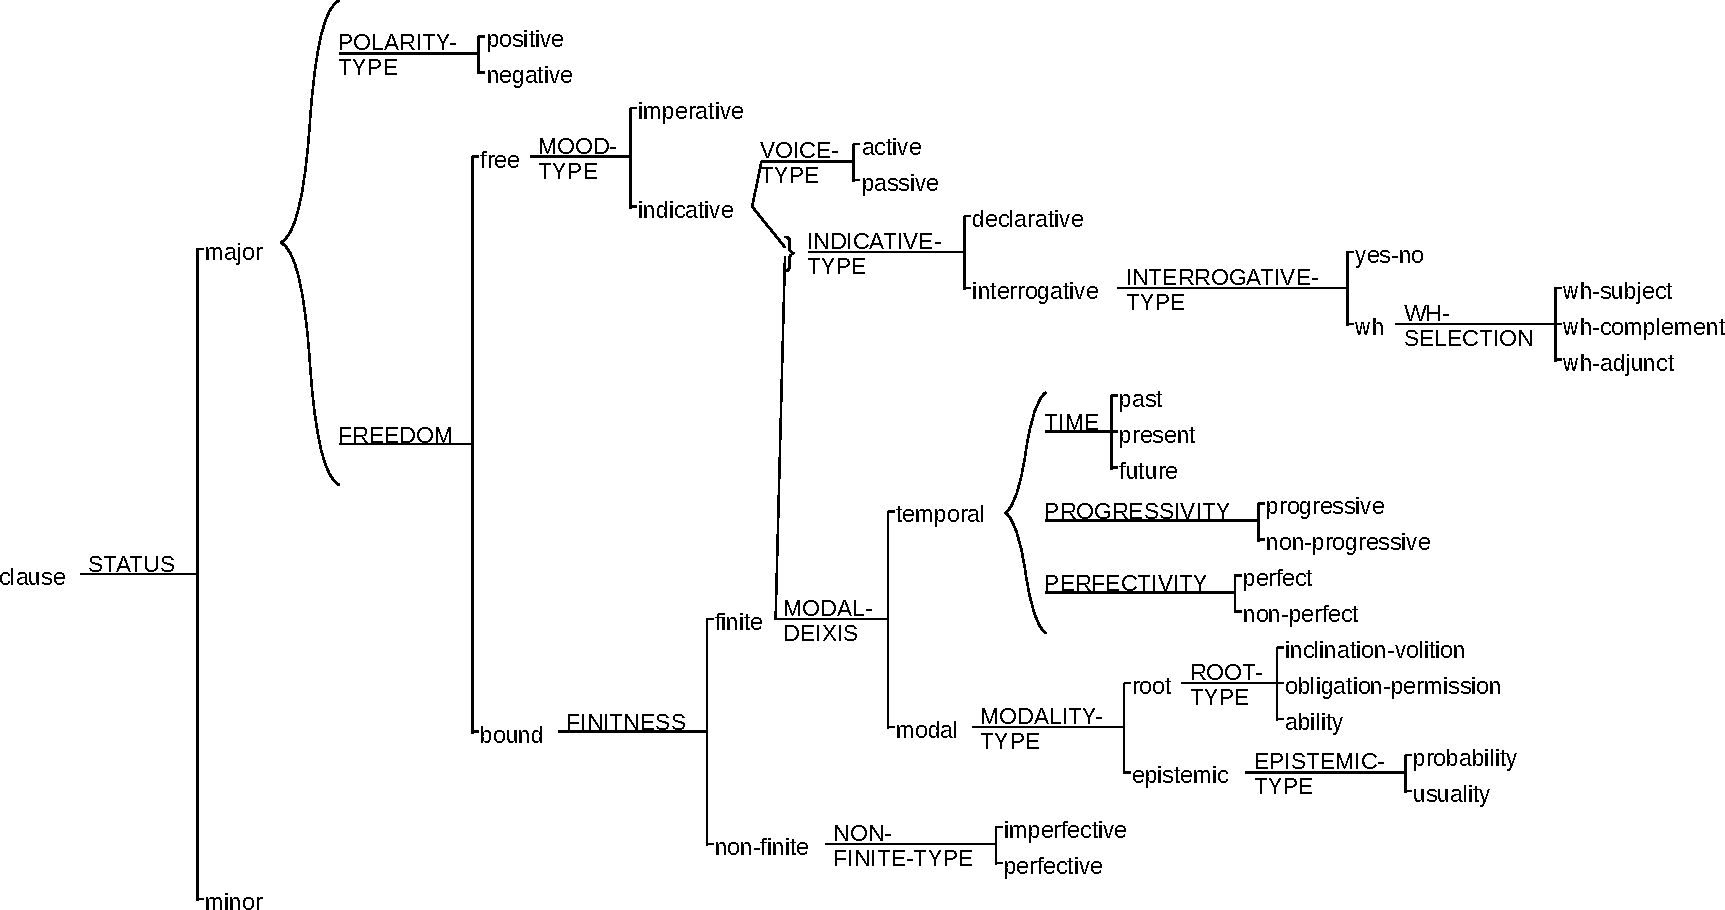
\includegraphics[width=\linewidth]{Figures/SFL-grammar/mood-simplified.pdf}
        \caption{An adaptation of the MOOD system network \citep[162]{Halliday2013}}
        \label{fig:clause-mood}
    \end{figure}

    The features of this feature network apply to units of clause class only. Even if some features may be intuitive or I iterate briefly over each of them providing hints for identifying it. 
    
    The POLARITY system indicates whether the clause is affirmed or negated. The negative polarity is indicated, in English, by the presence of a clausal particle \textit{not} or \textit{n't}. It can also be signalled by similar negative markers in other clause elements such as the subject (e.g. ``None of the kids came to play.''), adjunct (e.g. ``He is never coming back.'') or complement (e.g. ``She loves no one.''). In present work I consider the clausal negative marker only. 
    
    VOICE in the traditional grammar indicates, for transitive verbs, whether subject acts (\textit{active} voice) or is acted upon (\textit{passive} voice). In passive voice the subject and complement change position and the former is introduced by the preposition \textit{by}. 
    
    The semantics of FREEDOM system is to indicate whether the clause is \textit{free} and realises a proposition or proposal and serves to develop exchange in a dialogue either by initiating or responding to a speech act. On the other hand the \textit{bound} clauses are not open to negotiation and serve as supporting information to be taken for granted. Structurally, the bound clauses usually depend on a dominant one that is free.
    
    FINITENESS system indicates whether the clause is \textit{finite}, i.e. something that can be argued about. The way to make it arguable is by providing a point of reference into here and now (\textit{temporal}) or into the speaker's judgement (\textit{modal}). The latter two features constitute the MODAL-DEIXIS system. 
    
    The MODALITY-TYPE system is an adaptation from \citep[689--692]{Halliday2013} that focuses on the usage of the modal verbs only and is organised into ROOT and EPISTEMIC modalities. The former one comprises \textit{inclination-volition}, \textit{obligation-permission} and \textit{ability} while the latter of \textit{usuality} and \textit{probability} features.
    
    Temporal feature indicates that the clause has a tense. For simplicity, I replaced the Sydney account for tense with   that of traditional grammar of English. The systematisation is on three systems, that of TIME (past, present or future), PROGRESSIVITY (progressive or non-progressive) and PERFECTIVITY (perfect or non-perfect).    
    
    In addition to MOOD system network I include into the parsing process the DEIXIS system network for the nominal groups determination depicted in Figure \ref{fig:ng-determination}. The nominal DEIXIS system network is described in detail in IFG4 at the nominal group section \citep[364--396]{Halliday2013}. 
    
    \begin{figure}[!ht]
        \centering
        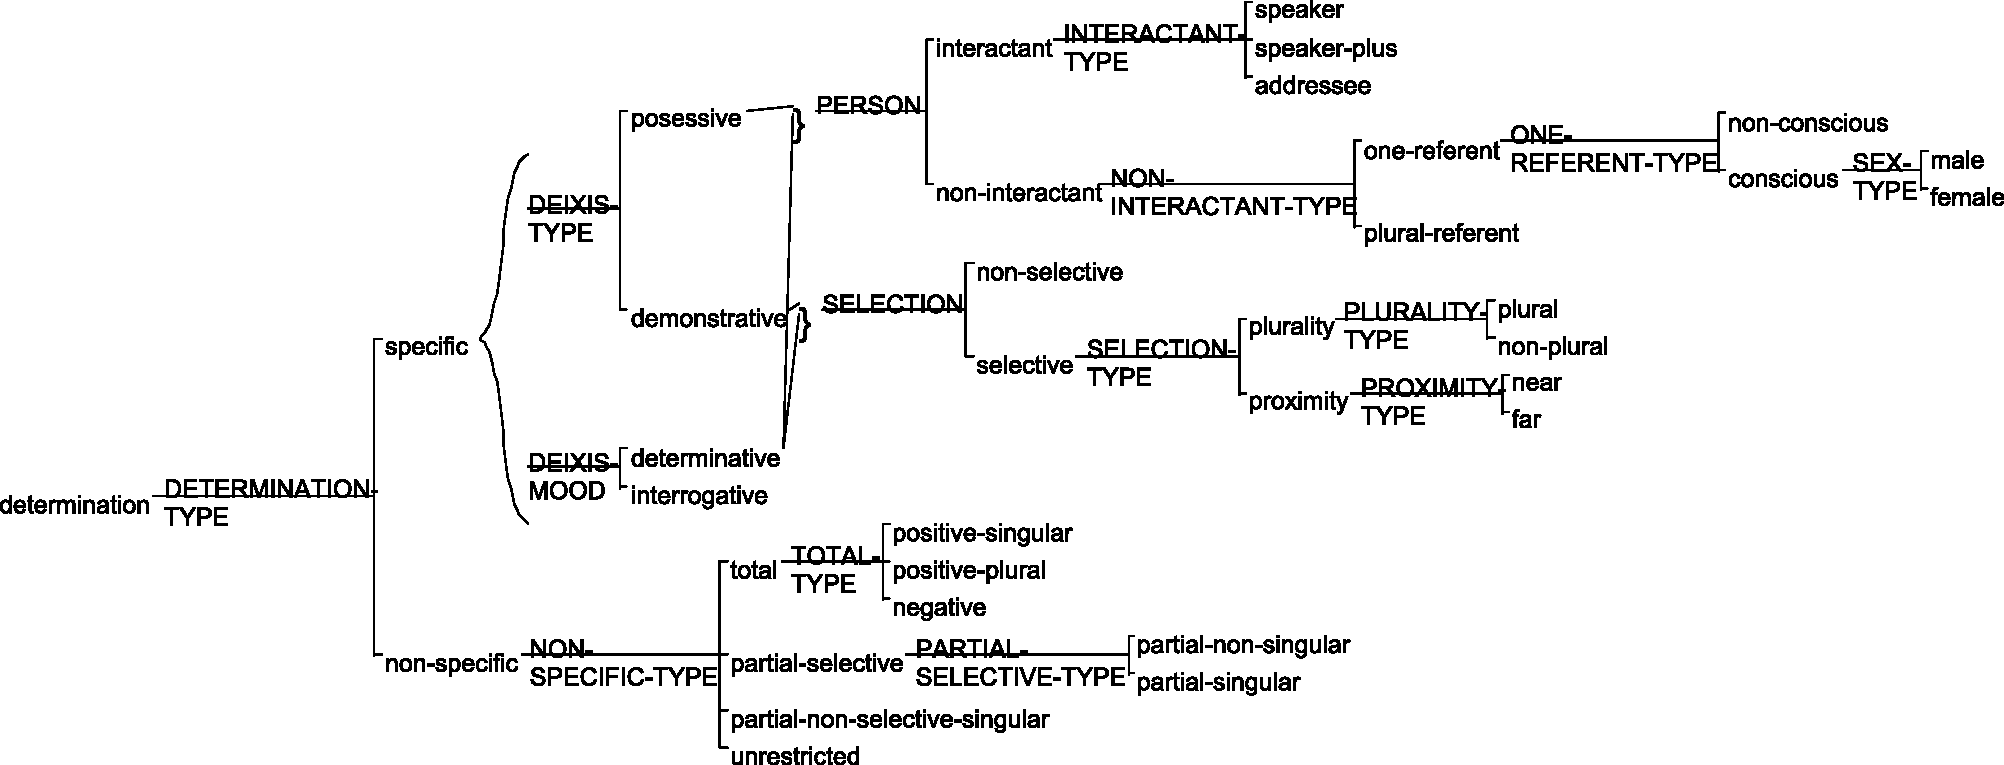
\includegraphics[width=\linewidth]{Figures/SFL-grammar/determination-system.pdf}
        \caption{The DEIXIS system network for the nominal group determination \citep[366]{Halliday2013}}
        \label{fig:ng-determination}
    \end{figure}

    This system network is relevant for the current work because determining the systemic selections for the entire network can be unambiguously done based on lexical information only. In Section \ref{sec:enrichment-stage}, we will see a dictionary lookup method in addition to graph pattern matching to determine systemic selections. Next is briefly described the system network of TRANSITIVITY. 
      
\subsection{TRANSITIVITY}
\label{sec:transitivity}
In Section \ref{sec:functions-metafunctions}, I explained that SFL organises the lexicogrammar in three metafunctions conflated with each other. This section briefly reminds of the experiential metafunction and introduces the TRANSITIVITY system network that systematizes it.

In this perspective, ``the clause construes a quantum of change in a flow of events as a \textit{figure}, or a configuration of a \textit{process}, \textit{participants} involved in it and any attendant \textit{circumstance}`` \citep[212]{Halliday2013}. 

In traditional grammar the term \textit{transitivity} refers to the property of verbs according to which they are classified into transitive and intransitive. In SFL the term transitivity is primarily concerned with clauses. It is most insightful to refer to Halliday's TRANSITIVITY \citep{Halliday67-parts1+2,Halliday68-part3,Halliday68} that deals with Predicate, Subject, Complement, and Adjunct all of which are elements of the clause and are usually conflated with the Process, Participants and Circumstances. 

Sydney grammar makes a distinction between two types of experience: ``inner'' as experience inside ourselves and ``outer'' as experience in the world around us. The prototypical outer experience is that of actions and events. The inner experience is more difficult to sort but it is a kind of reply of the outer, recording it, reflecting on it, reacting on it etc. Two grammatical categories that realize these sort of experiences are the \textit{material} process and \textit{mental} process.

In addition to material and mental there is a third kind of process used in identifying, classifying and relating various kinds of experience. The grammatical category realizing this type of links is the \textit{relational} process. Then using the combinations of the three main processes above, Halliday defines \textit{behavioural}, \textit{verbal} and \textit{existential} processes. 

\begin{figure}[!ht]
    \centering
    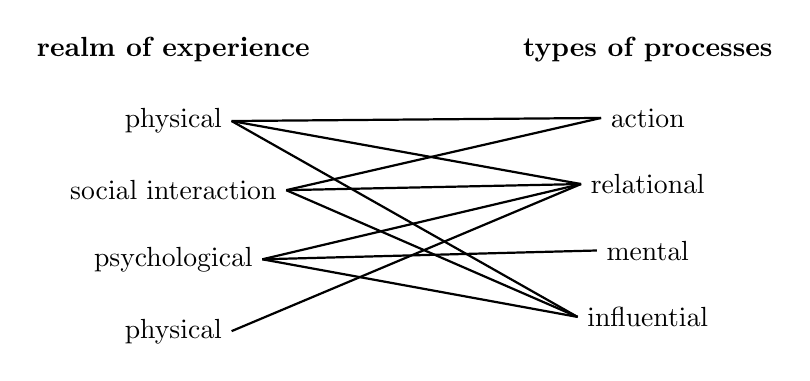
\begin{tikzpicture}[]
    \node (re) [font=\bf] {realm of experience};
    \node (ph) [below=1em of re] {physical};
    \node (si) [below=1em of ph] {social interaction};
    \node (ps) [below=1em of si] {psychological};
    \node (ab) [below=1em of ps] {physical};

    \node (pt) [font=\bf, right=7em of re] {types of processes};
    \node (ac) [below=1em of pt] {action};
    \node (re) [below=1em of ac] {relational};
    \node (me) [below=1em of re] {mental};
    \node (in) [below=1em of me] {influential};        
    
    \draw [thick] (ph.east) -- (ac.west);
    \draw [thick] (ph.east) -- (re.west);
    \draw [thick] (ph.east) -- (in.west);
    
    \draw [thick] (si.east) -- (ac.west);
    \draw [thick] (si.east) -- (re.west);
    \draw [thick] (si.east) -- (in.west);
    
    \draw [thick] (ps.east) -- (me.west);
    \draw [thick] (ps.east) -- (re.west);
    \draw [thick] (ps.east) -- (in.west);
    
    \draw [thick] (ab.east) -- (re.west);

    \end{tikzpicture}
    \caption{The connections in Cardiff grammar between realms of experience and the process types}
    \label{fig:cardiff-realm-processtype}
\end{figure}

\begin{figure}[!ht]
    \centering
    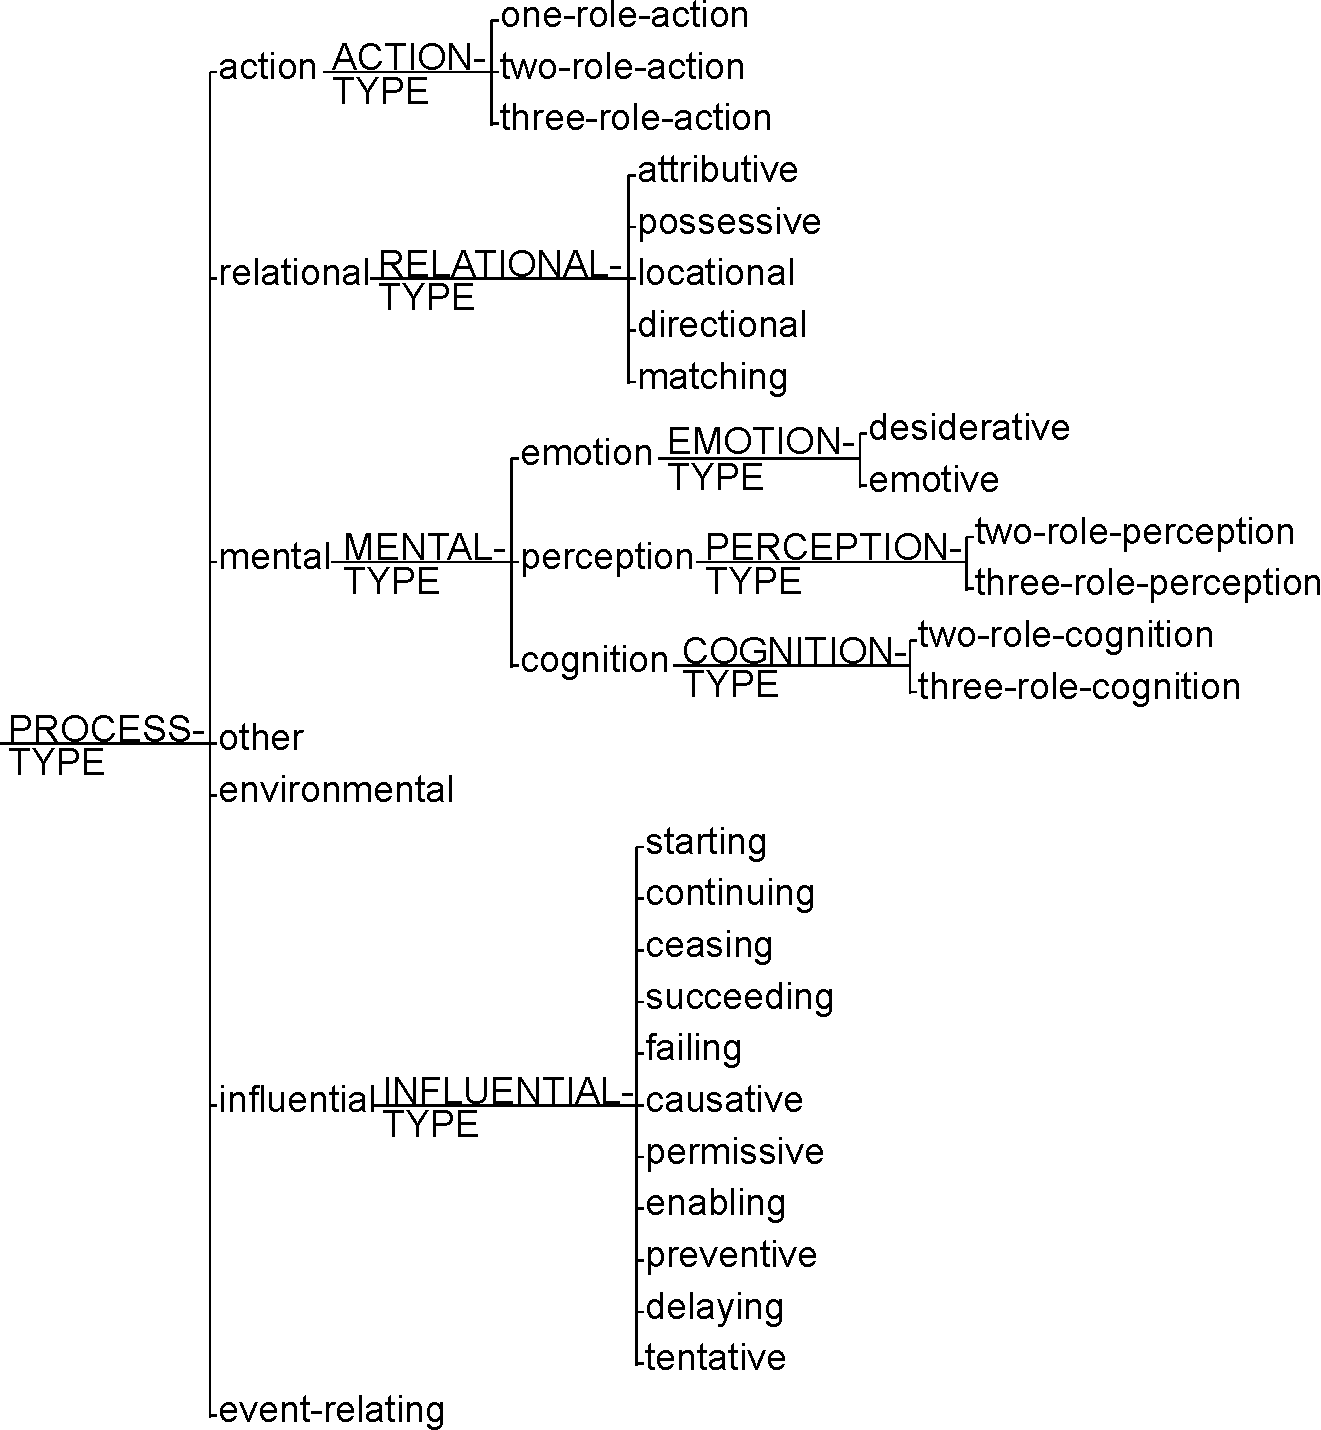
\includegraphics[width=0.8\linewidth]{Figures/SFL-grammar/Transitivity.pdf}
    \caption{Cardiff TRANSITIVITY system network}
    \label{fig:cardiff-transitivity}
\end{figure}

Cardiff grammar employs similar process types, that of \textit{action}, \textit{relational}, \textit{mental} and \textit{influential}. In addition, it links these process types to realms of experience: \textit{physical}, \textit{social interaction}, \textit{psychological} and \textit{abstract}.
Figure \ref{fig:cardiff-realm-processtype} provides the schematic connection between realms of experience and various process types that can realise that kind of experience \citep[37]{Fawcett2009}. 

\citet{Fawcett1973,Fawcett87-relational,Fawcett96} wrote the most on the TRANSITIVITY of Cardiff grammar. It is a model that evolved over time and is depicted in Figure \ref{fig:cardiff-transitivity} in its latest form. The first main process type is the \textit{action}. It has been called ``material process'' in the past, but Fawcett returned to use the term ``action'' because there are many actions that are non material, social for instance. The second main process is the \textit{relational} one that is subdivided into \textit{attributive}, \textit{posessive}, \textit{locational}, \textit{directional} and \textit{matching}.

The third main distinctions is the \textit{mental} process that if fine-grained into \textit{emotion}, \textit{perception} and \textit{cognition} distinctions. \textit{Environmental} processes, even if very rare, are recognised as another main process type. \textit{Influential} processes are unique to Cardiff grammar and not accounted elsewhere in the TRANSITIVITY system. All these processes have a structural similarity, that of having an embedded event into the matrix process and which is somehow influenced. The last process type is that of \textit{event-relating} which is also very new and specific to Cardiff grammar. All the linguistic phenomena covered by this process are treated by Halliday as grammatical metaphors, but Fawcett considered that they shall be analysed as a distinct process type.

The TRANSITIVITY system is highly dependent on the lexical semantics of the verbs. Therefore a vast account of verb senses and the participant configuration structure they command has to be provided in the grammar. \citet{Neale2002} has pioneered such work in her thesis which I introduce in the next Section. 

\subsection{Process Type Database}
\label{sec:ptdb-description-technical}

The Process Type Database (PTDB) \citep{Neale2002} is the key resource in the automatic Transitivity analysis developed in this work and described in Chapter \ref{ch:enrichment-stage}. It is also the source for creating the graph patterns used to enrich the constituency graph as described in the same chapter. PTDB provides information on what possible process types and participants can correspond to a particular verb meaning. The PTDB is a dictionary-like dataset of verbs bound to an exhaustive list of verb senses and the corresponding Process Configuration for each of them.

In her work on PTDB \citet{Neale2002} improved the TRANSITIVITY system of the Cardiff Grammar by systematizing over 5400 senses (and process configurations) for  2750 most popular English verbs. Table \ref{tab:example-ptdb} presents a simplified sample of PTDB content.

\begin{table}[!ht]
    \centering
    \resizebox{0.995\textwidth}{!}{%    
    \begin{tabulary}{1.2\textwidth}{|c|C|c|c|}
        \hline
        \textbf{verb form} & \textbf{informal meaning} & \textbf{process type} & \textbf{configuration} \\ \hline
        calculate & work out by mathematics (commission will then,calculate the number of casted votes) & cognition & Ag-Cog + Ph \\ \hline
        & plan (newspaper articles were calculated to sway reader's opinions) & two role action & Ag + Cre \\ \hline
        catch & run after and seize (a leopard unable to catch its normal prey) & possessive & Ag-Ca + Af-Pos \\ \hline
        & fall ill (did you catch a cold?) & possessive & Ag-Ca + Af-Pos \\ \hline
        catch (up with) & reach (Simon tried to catch up with others) & two role action & Ag + Ra \\ \hline
    \end{tabulary}
    }
    \caption{An example of records ins PTDB}
    \label{tab:example-ptdb}
\end{table}

The internal structure of the PTDB is detailed in Neale's PhD thesis \citep[193--231]{Neale2002}. In this thesis only three columns are of interest for the parsing purpose: the \textit{verb form} (1^{st}), the Cardiff grammar \textit{process type} (6^{th}) and the participant role \textit{configuration} (8^{th}). The content of these columns is not uniform and unsuitable for parsing purposes in its original form available on Neale's personal page\footnote{see \url{http://www.itri.brighton.ac.uk/~Amy.Neale/}}. The work on normalising and cleaning up the PTDB is described in Section \ref{sec:claning-ptdb}.


\section{Concluding remarks}
This chapter has described the grammatical units and the two system networks adopted in this work. They constitute a selection from from Sydney and Cardiff grammar implemented in the Parsimonious Vole parser.

Because of its bottom up approach to unit structure, rank scale relaxation and accommodation of embedding as a general principle, Cardiff systemic functional theory is more suitable for parsing than the Sydney one. Nonetheless the unit definitions in the Cardiff grammar are deeply semantic in nature. Parsing with such units requires most of the time lexical-semantically informed decisions beyond merely syntactic variations. This is one of the reasons why the parsing attempts by \citet{ODonoghue1991a} and others in the COMMUNAL project were all based on a corpus. It is also the reason to adapt in this thesis Sydney unit structures as they are closer to traditional grammar syntax \citep{Quirk1985}.

Next chapter lays the theoretical foundations of Dependency Grammar and introduces the Stanford dependency parser used as a departing point in current parsing pipeline (see Section \ref{sec:architecture}). Because there is a transformation step from dependency to systemic functional consistency structure, the next chapter also covers a theoretical compatibility analysis and how such a transformation should in principle look like. 


% \chapter{Dependency grammar (DG)}
\label{ch:dependecy-grammar}

The Stanford dependency analysis of a given text constitutes the input for the algorithm developed in the current work. It provides the foundation to build the syntactic backbone used adopted here. This chapter offers an overview of the grammar and the parser developed at the Stanford university. In the last part of the chapter is discussed the cross theoretical connection between the dependency and systemic functional grammars. 

\section{Origins of the dependency theory}
\label{sec:origins}
%In this section I outline the theory of dependency grammar. I will make references sometimes to concepts in SFG. 
For the first time a complete linguistic theory based on the dependency concept was elaborated by the French linguist Lucien Tesniere in his seminal work \textit{``Elements de syntaxe strusturale''} published in \citeyear{Tesniere59} after his death. He devoted much effort to argue for the adequacy of \textit{dependency} as the organizational principle underlying numerous phenomena and in fact attempting to demonstrate the universality of his syntactic analysis method for human languages. In doing so he introduced a series of concepts and ideas among which the \textit{verb centrality}, \textit{stratification}, \textit{language typology}, \textit{nuclei}, \textit{valency}, \textit{metataxis}, \textit{junction} and \textit{transfer} are the most important ones which I introduce following the connections.

%His work, originally in French, has been translated in multiple languages German, Russina, Spanish, Japanese, Italian and recently in English \citep{Tesniere2015}.

\begin{quotation}
    The sentence is an \textit{organized set}, the constituent elements of which are the words. Each word in a sentence is not isolated as it is in the dictionary. The mind perceives \textit{connections} between a word and its neighbours. The totality of these connections forms the scaffold of the sentence. These connections are not indicated by anything. But it is absolutely crucial that they be perceived by the mind; without them the sentence would not be intelligible \citep[3]{Tesniere2015}.
\end{quotation}

Tesniere holds the view that the connection, what is know today as \textit{dependencies}, are the foundations of the \textit{structural syntax} known as \textit{dependency grammar} today. According to him ``to construct a sentence is to breathe life into an amorphous mass of words, establishing a set of connections between them. Conversely, understanding a sentence involves seizing upon the set of connections that unite the various words'' \citep[4]{Tesniere2015}. He introduces the hierarchy of connections as follows. 

\begin{quotation}
    Structural connections establish \textit{dependency} relations between words. In principle, each connection unites a superior term and an inferior term. The superior term is called the \textit{governor}, and the inferior term the \textit{subordinate}. We say that the subordinate depends on the governor and that the governor governs the subordinate. [\dots] A word can be both subordinate to a superior word and governor of an inferior word. [\dots] The set of words of a sentence constitutes a veritable \textit{hierarchy} \citep[5--6]{Tesniere2015}.
\end{quotation}

Introduction of hierarchy and governor-subordinate dependencies permeates to define now what is a \textit{node} and the \textit{stemma} resembling what is now known as \textit{dependency tree} (although the stemmas do not include labels on the tree edges). 

\begin{quotation}
    [\dots] In principle, a subordinate can only depend on a sole governor. A governor, in contrast, can govern multiple subordinates [\dots] Every governor that governs one or more subordinates forms what we call a node. [\dots] it follows that \textit{each subordinate shares the fate of its governor} \citep[6]{Tesniere2015}.
\end{quotation}

\begin{figure}[!ht]
    \centering
    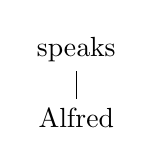
\begin{tikzpicture}
    \node[] (speaks) {speaks};
    \node[below=1em of speaks] (alfred) {Alfred};
    \draw[] (speaks) -- (alfred);
    \end{tikzpicture}
    \caption{Stemma for ``Alfred speaks''}
    \label{fig:stemma1}
\end{figure}

This asymmetry of connection permits construction of a tree-like structure. The diagram of the two word sentence ``Alfred speaks'' is provided in the Figure \ref{fig:stemma1}. The word ``speaks'' is the governor of the word ``Alfred''. The connection is depicted bu the vertical line connecting the two. But to make it complete it is important to decide on the root node. 

\begin{quotation}
    The node formed by the governor that governs all the subordinates of a sentence is the \textit{node of nodes}, or the central node. It is at the centre of the sentence and ensures its structural unity by tying the diverse elements into a single bundle. It can be identified with a sentence. \textit{The node of nodes is generally verbal} [\dots] \citep[7]{Tesniere2015}
\end{quotation}

% the verb centrality
The fundamental insight presented above about the nature of the syntactic structure concerns the grouping of words at the clause level. Tesniere rejects the subject-predicate formation that was the de facto syntactic understanding of his time. He argued that this division is belongs to Aristotelian logic and is not associated to linguistics. Instead of the subject-predicate division Tesniere positions the verb at the root of the clause structure making the subject and the object subordinated seedlings. Figure \ref{fig:stemma2} depicts the clause structure ``Alfred speaks slowly'' where both the subject and the object are subordinated to the central verb speaks. 

\begin{figure}[!ht]
    \centering
    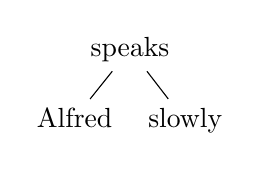
\begin{tikzpicture}
    \node[] (speaks) {speaks};
    \node[below=1em of speaks, xshift=-2em] (alfred) {Alfred};
    \node[below=1em of speaks, xshift=2em] (slowly) {slowly};
    \draw[] (speaks) -- (alfred);
    \draw[] (speaks) -- (slowly);
    \end{tikzpicture}
    \caption{Stemma for ``Alfred speaks slowly''}
    \label{fig:stemma2}
\end{figure}

% stratification
Tesniere is among pioneer linguists recognising that the language is organised at different levels thus advocating a \textit{stratified model of language}. He recognises the to dimensional syntactic representation and the one dimensional chain of spoken language. 

\begin{quotation}
    \textit{speaking} a language involves transforming structural order to linear order, and conversely, \textit{understanding} a language involves transforming linear order to structural order. The fundamental principle of transforming structural order to linear order involves changing the connections of structural order into the sequences of linear order. This transformation occurs in such a manner that the elements connected in structural order become immediate neighbours in the spoken chain \citep[12]{Tesniere2015}.
\end{quotation}

% syntax semantix difference
In the structural realm Tesniere goes even deeper and describes the separation between syntax and semantics. To argue for that, he uses an example similar to the famous Chomskian \textit{colourless green ideas sleep furiously} \citep{Chomsky57} (that occurred three years after Tesniere's death). He employed the sentence \textit{the vertebral silence antagonizes the lawful sail}.

\begin{quotation}
    Syntax is distinct from morphology, and it is no less distinct from semantics. The structure of a sentence is one thing, and the idea that it expresses and that constitutes its meaning is another. It is therefore necessary to distinguish between the structural plane and the semantic plane.
    [\dots]
    The structural plane and the semantic plane are therefore entirely independent of each other from a theoretic point of view. The best proof is that a sentence can be ­semantically absurd and at the same time syntactically perfectly correct \citep[33]{Tesniere2015}.
\end{quotation}

% nodes and nuclei
Tesniere distinguishes between \textit{nodes} and \textit{nuclei}. Initially he defines the node in a way that resembles the phrase or a constituent but after that he changes his mind.  

\begin{quotation}
    we define a \textit{node} as a set consisting of a governor and all of the subordinates that are directly or indirectly dependent on the governor and that the governor in a sense links together into a bundle \citep[6]{Tesniere2015}.
\end{quotation}

Latter in the book, he uses the term node to mean merely a vertex and even redefines it saying that ``The node is nothing more than a geometric point whereas the nucleus is a collection of multiple points \dots'' \cite[39]{Tesniere2015}. It is perhaps the inconsistent use of the terminology that lead to the assumption that the dependency grammar does not recognises phrases (i.e. that is the complete subtree of a vertex). In fact he defines nucleus as playing the role of both a semantic and syntactic unit.

\begin{quotation}
    We define the nucleus as the set which joins together, in addition to the structural node itself, all the other elements for which the node is the structural support, starting with the semantic elements \citep[38]{Tesniere2015}.
\end{quotation}

%valency
A notable contribution to the field of syntax is the concept of \textit{valency}. It is the notion used in other linguistic schools as \textit{transitivity} to express combinatorial properties of verbs and other lexical items. Inspired from natural sciences, Tesniere compares the relationship between verbs and the so called \textit{actants} (a.k.a. \textit{arguments}) to atom's bonds. 

\begin{quotation}
    The verb may therefore be compared to a sort of atom, susceptible to attracting a greater or lesser number of actants, according to the number of bonds the verb has available to keep them as dependents. The number of bonds a verb has constitutes what we call the verb’s \textit{valency} \citep[241]{Tesniere2015}.
\end{quotation}

%He distinguishes \textit{avalent}, \textit{monovalent}, \textit{bivalent} and \textit{trivalent} verbs. 
Atoms are not the only metaphor he uses and next I present another one regarding the \textit{verbal node} that is especially important for showing the syntax-semantics interplay. 

\begin{quotation}
     The verbal node, found at the centre of the majority of European languages, is a theatrical performance. Like a drama, it obligatorily involves a \textit{process} and most often \textit{actors} and \textit{circumstances}. [\dots] Transferred from the theatre to structural syntax, the process, the actors, and the circumstances become respectively the \textit{verb}, the \textit{actants}, and the \textit{circumstants} \citep[97]{Tesniere2015}.
\end{quotation}

Comparison of the verb to an atom seems to emphasize connection to the syntactic aspect of valency while comparing it to a theatrical performance seems to emphasize the semantic properties of valency. Therefore his theory of valency has semantic and syntactic properties. He believed that the first actant is the agent of the action, identified as the subject in traditional grammar, and the second actant is the one that bears the action, identified as the syntactic object. Tesniere regards both of them as complements to complete the governor verb making, in this sense, the subject indistinguishable from other complements. 

%junction
There are some phenomena that are deemed quite problematic, namely they are the \textit{coordination} or \textit{apposition}. They constitute a challenge because they are not governor-subordinate relations but are rather orthogonal relations among siblings. Tesniere analyses the coordination, or as he calls it \textit{junction}, as a phenomena used in language to express (semantic) content efficiently. 

He viewed the junction as fundamentally different from the subordination  and represented it with horizontal lines. Subordination is a principle of organization on the vertical axis whereas the coordination (i.e. junction) on the horizontal axis. Figure \ref{fig:stemma3} depicts two example representations for the sentence ``Young boys and girls played'' and ``Alfred adores cookies and detests punishments''. 

\begin{figure}[!ht]
    \centering
    \begin{subfigure}{.35\textwidth}
        \centering
        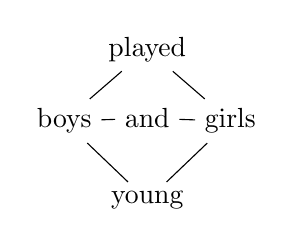
\begin{tikzpicture}
        \node[] (played) {played};
        \node[below=1em of played, xshift=-3em] (boys) {boys};
        \node[below=1em of played, xshift=0em] (and) {and};
        \node[below=1em of played, xshift=3em] (girls) {girls};
        \node[below=4em of played, xshift=0em] (young) {young};
        \draw[] (played) -- (boys);
        \draw[] (played) -- (girls);
        \draw[] (and) -- (girls);
        \draw[] (and) -- (boys);    
        \draw[] (young) -- (boys);
        \draw[] (young) -- (girls);
        \end{tikzpicture}
        \caption{Young boys and girls played}
        \label{fig:stemma3-sub1}
    \end{subfigure}%
    \begin{subfigure}{.65\textwidth}
        \centering
        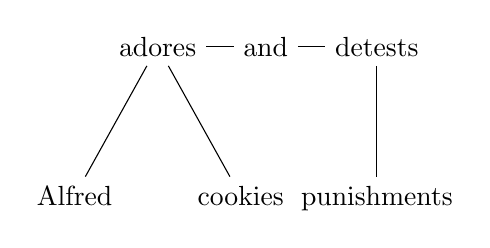
\begin{tikzpicture}
        \node[] (adores) {adores};
        \node[right=1em of adores] (and) {and};
        \node[right=1em of and] (detests) {detests};
        \node[below=4em of adores, xshift=-3em] (alfred) {Alfred};
        \node[below=4em of adores, xshift=3em] (cookies) {cookies};
        \node[below=4em of detests, xshift=0em] (pun) {punishments};
        \draw[] (adores) -- (alfred);
        \draw[] (adores) -- (cookies);
        \draw[] (and) -- (adores);
        \draw[] (and) -- (detests);    
        \draw[] (detests) -- (pun);
        \end{tikzpicture}
        \caption{Alfred adores cookies and detests punishments}
        \label{fig:stemma3-sub2}
    \end{subfigure}
    \caption{Sample stemmas with \textit{junction} representation}
    \label{fig:stemma3}
\end{figure}

%The junction is total when the conjuncts shared their heads and/or dependents and partial when some are not shared. For the total junction Tesniere used terms of heraldry: \textit{coped} (upwards triangle formed by two conjuncts sharing a dependant), \textit{shod} (downwards triangle formed by a head governing two conjuncts) and \textit{dressed} (diamond formed by conjuncts with one shared head and one shared dependant). The partial structures are called \textit{bifid} are asymmetric one way or another and are classified as \textit{anadidymic}, \textit{catadidymic}, \textit{anacatadidymic}

%transfer
A big part of the Tesniere's \textit{Elements} \citep{Tesniere59} is dedicated to the theory of \textit{transfer}. It describes the phenomena when one class of a syntactic unit occupies a position usually devoted to another one. In SFL it is called the grammatical metaphor defined in \ref{def:gramatical-metaphor}. For example the noun can be transferred to an adjective by preposition ``of'', as for example \textit{a linguist of France} where the source \textit{France} is transferred to target \textit{of France} which modify \textit{linguist} that is typically an adjectival function. Transfer is a tool that explains how for example a clause can be embedded into another one or how a verb can be subordinate to another one. 

Tesniere splits the words into \textit{function words} or \textit{translatives} (i.e. prepositions, conjunctions, auxiliary verbs and articles) and four basic categories of \textit{content words} (i.e. verbs (I), nouns (O), adverbs (E) and adjectives (A) ). The former are empty of content marker transfer of content words from one syntactic category to another one. That is, allowing one word to occupy a position that is generally associated with a word of another category. 

One distinguishing trait of the transfer is that the words transferred from source to target category continue to behave as the source category with respect to their dependants and as source category to its governor.

The transfer theory is controversial for the translators of the Elements. They write \citep[liv-lx]{Tesniere2015} that while the transfer schema can not be interpreted in terms of pure dependency it is debatable whether it can be interpreted in terms of constituency. The main distinction is in the number of nodes that one assumes to be in the syntactic structure i.e. whether there are intermediary virtual nodes. 

\begin{figure}[!ht]
    \centering
    \begin{subfigure}{.33\textwidth}
        \centering
        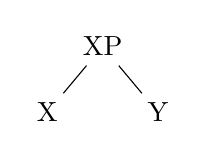
\begin{tikzpicture}
        \node[] (XP) {XP};
        \node[below=1em of XP, xshift=-2em] (X) {X};
        \node[below=1em of XP, xshift=2em] (Y) {Y};
        \draw[] (XP) -- (X);
        \draw[] (XP) -- (Y);
        \end{tikzpicture}
        \caption{Headed endocentric}
        \label{fig:stemma4-sub1}
    \end{subfigure}%
    \begin{subfigure}{.33\textwidth}
        \centering
         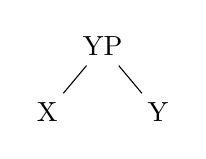
\begin{tikzpicture}
        \node[] (YP) {YP};
        \node[below=1em of YP, xshift=-2em] (X) {X};
        \node[below=1em of YP, xshift=2em] (Y) {Y};
        \draw[] (YP) -- (X);
        \draw[] (YP) -- (Y);
        \end{tikzpicture}
        \caption{Headed endocentric}
        \label{fig:stemma4-sub2}
    \end{subfigure}
    \begin{subfigure}{.33\textwidth}
        \centering
     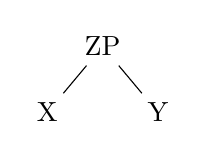
\begin{tikzpicture}
        \node[] (XP) {ZP};
        \node[below=1em of XP, xshift=-2em] (X) {X};
        \node[below=1em of XP, xshift=2em] (Y) {Y};
        \draw[] (XP) -- (X);
        \draw[] (XP) -- (Y);
    \end{tikzpicture}
    \caption{Non-headed exocentric}
    \label{fig:stemma4-sub3}    
    \end{subfigure}
    \caption{Constituency structure}
    \label{fig:stemma4}
\end{figure}

\begin{figure}[!ht]
    \centering
    \begin{subfigure}{.33\textwidth}
        \centering
        \begin{tikzpicture}
        \node[] (X) {X};
        \node[below=1em of X, xshift=2em] (Y) {Y};
        \draw[] (X) -- (Y);
        \end{tikzpicture}
        \caption{Headed endocentric}
        \label{fig:stemma5-sub1}
    \end{subfigure}%
    \begin{subfigure}{.33\textwidth}
        \centering
        \begin{tikzpicture}
        \node[] (X) {Y};
        \node[below=1em of X, xshift=-2em] (Y) {X};
        \draw[] (X) -- (Y);
        \end{tikzpicture}
        \caption{Headed endocentric}
        \label{fig:stemma5-sub2}
    \end{subfigure}
    \begin{subfigure}{.33\textwidth}
        \centering
        \begin{tikzpicture}
        \node[] (XP) {$\emptyset$};
        \node[below=1.2em of XP, xshift=-2em] (Y) { };
        \end{tikzpicture}
        \caption{Non-headed exocentric}
        \label{fig:stemma5-sub3}
    \end{subfigure}
    \caption{Dependency structure}
    \label{fig:stemma5}
\end{figure}


Figure \ref{fig:stemma4} shows how a sequence of two elements X and Y can be represented in terms of constituency where the Figure \ref{fig:stemma4-sub1} and \ref{fig:stemma4-sub2} represent that one element governs the other called \textit{endocentric} structures and in Figure \ref{fig:stemma4-sub3} a non-headed structure called \textit{exocentric}. Dependency structure depicted below in Figure \ref{fig:stemma5}, in contrast, cannot represent non-headed structures. Hence there is no correspondent dependency representation to Figure \ref{fig:stemma4-sub3} in Figure \ref{fig:stemma5-sub3}. 

Bringing back the discussion on the number of nodes, the constituency structure requires three nodes each time whereas dependency structure only two. In this sense the transfer schemas provided by Tesniere in his Elements \citep{Tesniere59} resembles constituency structure more than dependency structure simply because it assumes more nodes than words. 

%TODO compare transformation to the gramatical metaphor, see the definitiopn of the grammatical metaphor https://www.thoughtco.com/grammatical-metaphor-or-gm-1690913
%Elements - transaltors ppt - http://depling.org/depling2015/Tesniere.pdf
%Elements - transaltors intro - https://kahanedotfr.files.wordpress.com/2017/01/tesniere-introduction-benjamins2015.pdf


\section{Evolution into the modern dependency theory}
Nowadays the dependency theory differs from the original one presented by Tesniere. At the time the original text was written there was no such distinction as dependency and constituency structures and that Tesniere's Elements \citep{Tesniere59} in fact contains descriptions of and references to what may nowadays be considered constituency. 
Next I present which of the initial ideas did not take hold, were not addressed or merely assumed and instead have evolved into the modern dependency theory of grammar.

\subsection{Definition of dependency}
Tesniere's definition of dependency is not satisfiable. His mentalist approach that ``the mind perceives connections between the word and it's neighbours''\citep[3]{Tesniere2015} makes it impossible to falsify his choices hence leaving no means to validate one choice over the other ones.

One way to define dependency relations and structure is by employing the constituency concept. There are efforts by \citep{Bloomfield33,Hockett58,harris1951methods} in constituency grammar to identify constituents using tests that shed light on which segments should hold together as phrases or whether they should be considered constituents at all. One needs to decide within each constituent which word it is being headed by which means deciding which word controls the distribution of that constituent \citep{Bloomfield33,Zwicky85-heads} . A word \textit{y} depends of a word \textit{x} if and only if \textit{y} heads the a phrase which is an immediate constituent of the phrase headed by \textit{x} \citep{Lecerf1961}. 

Another way to define dependencies, avoiding constituency, is by using combinations of two words as proposed by \citet{Garde1977} and \citet{melcuk88}. To discern which governs the other one needs to determine which determined the distribution of the two together. This way the governor is the word that determines the environment in which the two together can appear \citep[lxi]{Tesniere2015}. In fact the word notion is not necessary to define dependency, it can be abstracted away to the notion of syntactic units. As soon as two units combine one can posit dependency between them whereby the dependency structure is the set of dependencies between the most granular syntactic units \citep{gerdes2013defining}.

In addition Tesniere did not make distinctions between the dependency types. As discussed in the previous section, he had noticed that there is a difference between syntactic and semantic dependencies and that the former generally corresponds to the latter but not as a strict rule and even some other times the correspondence is in the opposite direction e.g. ``the stone frees'' vs. ``the frozen stone''. The dependency based semantic representations have been around since '60s named \textit{semantic networks} \citep{ZolkovskijMelcuk67,melcuk88} and \textit{conceptual graphs} \citep{schank1969, Sowa1976}.

\subsection{Grammatical function} 
In the modern linguistics the notion of grammatical functions e.g. subject, object, determiner etc. are attached to the notion of syntactic dependency. They are in fact an essential account in the modern dependency-based approaches because they are the only way to distinguish between various roles the dependents play in relation to their governors. The grammatical functions attached to the dependency relations are primitives of the dependency grammars. This is not the case for Chomskian phrase structure constituency where the functions are derived from the structural configurations. Nevertheless in latter constituency models such as \textit{Lexical Functional Grammars} \citep{Brensan2000} and \textit{Head-Driven Phrase Structure} \citep{PollardSag1994} have introduces the grammatical functions as grammatical primitives.

The grammatical functions were not important in Tesniere's theory. He mentioned only, in the context of valency theory, three \textit{actant functions} called \textit{first}, \textit{second} and \textit{third} the other verb dependants being \textit{circumstantial}. Most dependecy grammars assume dozens of functions to offer a fine-grained syntactic characterization of language based on distinguishable syntactic properties. This way two elements have the same grammatical function if and only if they have the same \textit{markers,} \textit{order} (linear position), \textit{agreement properties} and \textit{distribution}. Several grammatical function sets have been developed in the fields of formal dependency grammars, parsers and tree-banks. The most important ones for English Language are the ones of \citet{MelcukPertsov86}, of \citet{Johnson2000} and of \citet{Marneffe2008, Marneffe2008a}. In this work is employed the latter as it is part of the Stanford dependency parser described latter in this Chapter. 

\subsection{Projectivity}
Central to how the word order is accounted for in dependency grammar is \textit{projectivity}. It is not present in the Elements but it is the basis for identifying \textit{long-distance dependencies} also known as \textit{discontinuities} or \textit{gapping}. The concept is introduced by \citet{Lecerf1961} following publication of the Elements \citep{Tesniere59}. It is defined in terms of crossing lines when drawing dependency trees where the ones without containing crossing lines are called \textit{projective} and the ones with crossing lines are called \textit{non-projective} i.e. violating projection principle. 

\begin{figure}[!ht]
    \centering
    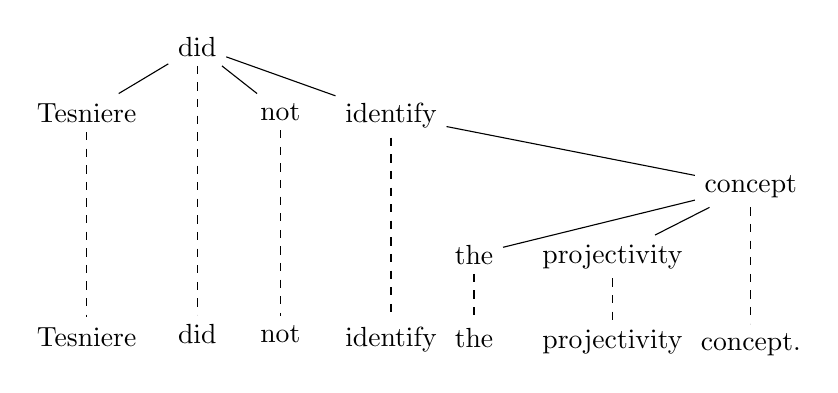
\begin{tikzpicture}
    \node[] (did) {did};
    \node[below=1em of did, xshift=-4em] (tesniere) {Tesniere};
    \node[below=1em of did, xshift=3em] (not) {not}; 
    \node[below=1em of did, xshift=7em] (identify) {identify}; 
    \node[below=1em of identify, xshift=13em] (concept) {concept}; 
    \node[below=1em of concept, xshift=-10em] (the) {the}; 
    \node[below=1em of concept, xshift=-5em] (projectivity) {projectivity}; 
    
    \node[below=9em of did] (did1) {did};
    \node[below=6.7em of tesniere] (tesniere1) {Tesniere};
    \node[below=6.7em of not] (not1) {not};
    \node[below=6.5em of identify] (identify1) {identify};
    \node[below=4.2em of concept] (concept1) {concept.};
    \node[below=1.6em of the] (the1) {the};
    \node[below=1.5em of projectivity] (projectivity1) {projectivity};
    
    \draw[] (did) -- (tesniere);
    \draw[] (did) -- (not);
    \draw[] (did) -- (identify);
    \draw[] (identify) -- (concept);
    \draw[] (concept) -- (the);
    \draw[] (concept) -- (projectivity);
    
    \draw[dashed] (did) -- (did1);
    \draw[dashed] (not) -- (not1);
    \draw[dashed] (tesniere) -- (tesniere1);
    \draw[dashed] (the) -- (the1);
    \draw[dashed] (concept) -- (concept1);
    \draw[dashed] (projectivity) -- (projectivity1);
    \draw[dashed] (identify) -- (identify1);
    
    \end{tikzpicture}
    \caption{Projective tree}
    \label{fig:stemma6}
\end{figure}

\begin{figure}[!ht]
    \centering
    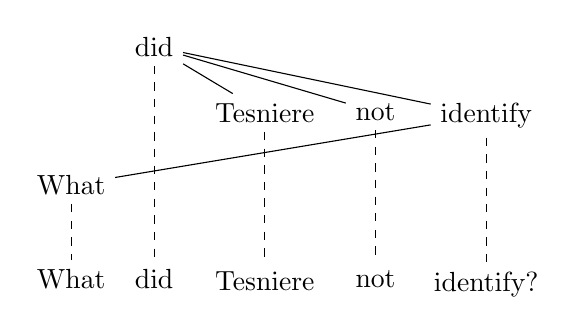
\begin{tikzpicture}
    \node[] (did) {did};
    \node[below=1em of did, xshift=4em] (tesniere) {Tesniere};
    \node[below=1em of did, xshift=8em] (not) {not}; 
    \node[below=1em of did, xshift=12em] (identify) {identify}; 
    \node[below=1em of identify, xshift=-15em] (what) {What};
    
    \node[below=7em of did] (did1) {did};
    \node[below=4.7em of tesniere] (tesniere1) {Tesniere};
    \node[below=4.7em of not] (not1) {not};
    \node[below=4.5em of identify] (identify1) {identify?};
    \node[below=2em of what] (what1) {What};
    
    \draw[] (did) -- (tesniere);
    \draw[] (did) -- (not);
    \draw[] (did) -- (identify);
    \draw[] (identify) -- (what);
    
    \draw[dashed] (did) -- (did1);
    \draw[dashed] (not) -- (not1);
    \draw[dashed] (tesniere) -- (tesniere1);
    \draw[dashed] (identify) -- (identify1);
    \draw[dashed] (what) -- (what1);    
    \end{tikzpicture}
    \caption{Non-projective tree}
    \label{fig:stemma7}
\end{figure}

To illustrate this principle consider Figure \ref{fig:stemma6} where there are no crossing lines whereas Figure \ref{fig:stemma7} contains projectivity violation because the word ``what'' is connected to it's governor ``identify'' crossing three dashed projection lines. Linguistic phenomena involving non-projecting are: wh-fronting, topicalization, scrambling, and extrapolation. 

\subsection{Function words}
Tesniere's transfer theory, despite it's insightfulness, has little if any at all application in modern dependency grammar. The main reason is the implications it has on the hierarchical structure because it does not provide the \textit{translatives} (prepositions, auxiliary verbs, sub-ordinators and conjunctions) with autonomy but a kind of secondary status and thus cannot be constitutive of a nucleus. The issue is reduced to the hierarchical status of such translatives whether they gain node status or not. 

\begin{figure}[!ht]
    \centering
    \begin{subfigure}{.33\textwidth}
        \centering
        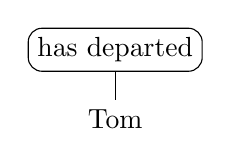
\begin{tikzpicture}
            \node[rounded corners=0.5em, draw] (has) {has departed};
            \node[below=1em of has] (tom) {Tom};
            \draw[] (tom) -- (has);
        \end{tikzpicture}
        \caption{}
        \label{fig:stemma8-sub1}
    \end{subfigure}%
    \begin{subfigure}{.33\textwidth}
        \centering
        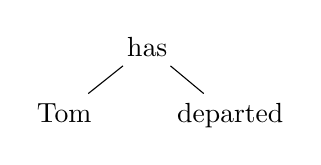
\begin{tikzpicture}
            \node[] (has) {has};
            \node[below=1em of has, xshift=-3em] (tom) {Tom};
            \node[below=1em of has, xshift=3em] (departed) {departed};
            \draw[] (tom) -- (has);
            \draw[] (departed) -- (has);
        \end{tikzpicture}
        \caption{}
        \label{fig:stemma8-sub2}
    \end{subfigure}
    \begin{subfigure}{.33\textwidth}
        \centering
        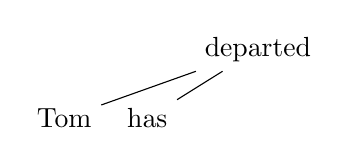
\begin{tikzpicture}
            \node[] (has) {departed};
            \node[below=1em of has, xshift=-7em] (tom) {Tom};
            \node[below=1em of has, xshift=-4em] (departed) {has};
            \draw[] (tom) -- (has);
            \draw[] (departed) -- (has);
        \end{tikzpicture}
        \caption{}
        \label{fig:stemma8-sub3}
    \end{subfigure}
    \caption{Possible analysis representation for ``Tom has departed''}
    \label{fig:stemma8}
\end{figure}

Figure \ref{fig:stemma8} represents three possible ways to analyse the word has in ``Tom has departed''. In Figure \ref{fig:stemma8-sub1} is represented the original approach Tesniere proposed using transfer schema where the word ``has'' is enclosed within the full verb node ``departed''. The two together are granted the status of a dissociated nucleus which means that neither alone can form a nucleus. In contrast the Figure \ref{fig:stemma8-sub2} and \ref{fig:stemma8-sub3} the auxiliary has is granted autonomy and corresponds to the modern analysis varying from one model to the other. 

As we will see in the next Section, the Stanford dependency schema \citep{Marneffe2008,Marneffe2008a} adopts the content words as governors of the function words. This corresponds to the representation in Figure \ref{fig:stemma8-sub3}. Moreover it provides a collapsed schema where the function words are suffixed to the grammatical functions. For example in ``Bob and Jacob'' there is a ``conj'' dependency relation between Jacob and Bob and a ``cc'' relation between ``and'' and ``Bob''. In the collapsed form the relation becomes ``conj:and'' between between Jacob and Bob integrating the conjunction into the relation name. This is the case for prepositions and conjunctives whereas auxiliary verbs remain nodes in the collapsed form. 

\section{Dependency grammar in automated text processing}
Tesniere had no intention in providing a computational theory of grammar and he was neither aware that ideas he was proposing have such potential. Shortly after his death, inspired by Chomsky's Syntactic Structure \citep{Chomsky57}, \citet{Hays1960,Hays1964} makes the first attempts to formalise the dependency grammar with intention to apply it to automated text processing. A year latter his colleague \citet{Gaifman1965} proofs that the \textit{dependency grammar} formalism proposed by Hays is equivalent to Chomsky's \textit{context free grammar} and to \textit{categorial grammars} proposed by \citet{BarHillel53}.

Outshined by Chomskyan grammars, the serious developments in parsing with dependency grammars did not come into being until mid '90s. First efficient parser with the dependency-based model called \textit{Link Grammar} was created by \citet{sleator1995parsing} and ten year latter the dependency parsing gain in popularity yielding remarkable results such as the MaltParser \citep{Nivre2006,Nivre2007parser}, MATE parser \citep{Bohnet2010} and early Stanford parser \citep{Marneffe2006} that was generating the dependency trees from phrase structure trees. A summary of dependency parsing techniques is provided by \citet{kubler2009dependency}.

In parallel to parsers, large annotated corpses and treebanks have been developed for parser training and testing and suitable as well for theoretical applications. A treebank is a collection of records consisting of natural language sentences associated with corresponding syntax tree (using a specific grammatical model) and optionally additional annotations such as part of speech tags, named entities, and other annotations. The first treebank was Penn Treebank \citep{Santorini1990,Marcus1993} which is a constituency-base treebank. A well known dependency treebank is the Prague Dependency Treebank \citep{hajic2001prague,Bohmova2003} originally created for Czech but now containing English as well. Recently started an initiative to create a Universal Dependency model \citep{nivre2015} and correspondingly with extended efforts was also created a multilingual treebank applying the scheme \citep{Nivre2016ud} which continues growing today.

%TODO introduce GR and PARK schemes

Before arriving to the broadly accepted Universal Dependency, early dependency grammars were quite dispersed. The schemes more often were developed in the context of corpus annotation. An early work \citep{carroll1998parser} towards unification was within the Grammar Evaluation Interest Group \citep{Harrison1991} also know as \textit{PARSEVAL} initiative that was originally destined for constituency parsers. \citet{Carroll1999} proposed an application independent corpus annotations scheme (see Figure \ref{fig:grEarly}) specifying the syntactic dependency which holds between each head and its dependent(s) that took into account language phenomena in English, Italian, French and German. 

\begin{figure}[!ht]
    \centering
    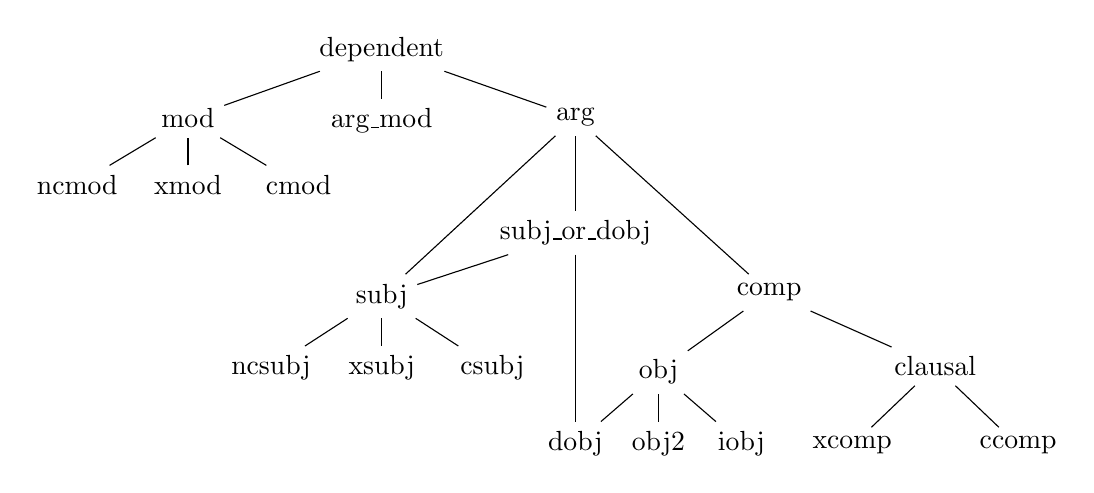
\begin{tikzpicture}
        \node[] (dependent){dependent};
        \node[below=1em of dependent, xshift=-7em] (mod){mod};
        \node[below=1em of dependent, xshift=0em] (argmod){arg\_mod};
        \node[below=1em of dependent, xshift=7em] (arg){arg};
        
        \node[below=1em of mod, xshift=-4em] (ncmod){ncmod};
        \node[below=1em of mod, xshift=-0em] (xmod){xmod};
        \node[below=1em of mod, xshift=4em] (cmod){cmod};
        
        \node[below=5em of arg, xshift=-7em] (subj){subj};
        \node[below=2.7em of arg, xshift=0em] (sodo){subj\_or\_dobj};
        \node[below=5em of arg, xshift=7em] (comp){comp};
        
        \node[below=1em of subj, xshift=-4em] (ncsubj){ncsubj};
        \node[below=1em of subj, xshift=0em] (xsubj){xsubj};
        \node[below=1em of subj, xshift=4em] (csubj){csubj};
        
        \node[below=1.4em of comp, xshift=-4em] (obj){obj};
        \node[below=1.3em of comp, xshift=6em] (clausal){clausal};
        
        \node[below=1em of obj, xshift=-3em] (dobj){dobj};
        \node[below=1em of obj, xshift=0em] (obj2){obj2};
        \node[below=1em of obj, xshift=3em] (iobj){iobj};
        
        \node[below=1.5em of clausal, xshift=-3em] (xcomp){xcomp};
        \node[below=1.5em of clausal, xshift=3em] (ccomp){ccomp};
        
        \draw[] (dependent) -- (mod);
        \draw[] (dependent) -- (arg);
        \draw[] (dependent) -- (argmod);
        
        \draw[] (ncmod) -- (mod);
        \draw[] (xmod) -- (mod);
        \draw[] (cmod) -- (mod);
        
        \draw[] (sodo) -- (arg);
        \draw[] (subj) -- (arg);
        \draw[] (comp) -- (arg);
        
        \draw[] (subj) -- (ncsubj);
        \draw[] (subj) -- (xsubj);
        \draw[] (subj) -- (csubj);
        
        \draw[] (subj) -- (sodo);
        \draw[] (sodo) -- (dobj);
        
        \draw[] (comp) -- (obj);
        \draw[] (comp) -- (clausal);
        
        \draw[] (dobj) -- (obj);
        \draw[] (obj2) -- (obj);
        \draw[] (iobj) -- (obj);
        
        \draw[] (xcomp) -- (clausal);
        \draw[] (ccomp) -- (clausal);
    \end{tikzpicture}
    \caption{The grammatical relations (GR) hierarchy from \citet{Carroll1999}}
    \label{fig:grEarly}
\end{figure}

In early 2000 the existing treebanks were still inadequate for evaluating the predicate-argument structure of English clauses. To address this problem, PARC 700 treebank \citep{King2003} was created by randomly extracting 700 sentences from Penn treebank, parsed with a Lexical Functional Grammar (LFG), converted into dependency relations and manually corrected by human validators. This scheme has played role in creation of Stanford dependency model that I describe in detail latter. 

%CoNLL
One advantage of dependency representations is that they can be encoded in a tabular format such as CoNLL \citep{nivre2007conll} which now is adopted as the standard representation. It is employed in a recurring open competition called ``CoNLL shared task'' launched for improving and innovating the dependency parsing methods. The most notable are the ones from 2006 on dependency parsing \citep{Buchholz2006} followed in 2007 that included a track for multilingual and one for domain specific dependency parsing. Fast forward to 2017 \citep{zeman2017conll} the task was for parsing from raw text (as previous ones were lemmatised and annotated with part of speech) into universal dependency.

\section{Stanford dependency model}
The functional dependency descriptions is precisely the aspect which makes possible the beneficial link between the Stanford Dependency Grammar and the Systemic Functional structures targeted in the current thesis. 

Stanford parser is one of the leaders in the domain of dependency parsing. Since 2006 \citep{Marneffe2006} for ten years Stanford parser implemented the Stanford dependency model for English (and a few other languages). Then in 2015 \citet{Nivre2016ud} proposes the language independent Universal Dependency scheme. In this section I present the Stanford dependency model (prior to Universal Dependency) that is used in the current parser. 

The design of the Stanford dependency set \citep{Marneffe2006, Marneffe2008,  Marneffe2014, Silveira2014} bears a strong intellectual debt to the framework of Lexical Functional Grammars \citep{Brensan2000} from which many relations  were adopted. \citet{Marneffe2006} departs from the relation typology described in \citep{Carroll1999} which was employed in PAREVAL initiative \citep{Harrison1991} and from the grammatical relations of PARC 700 \citep{King2003} scheme following a style of Lexical Functional Grammar. Marneffe arranges the grammatical relations into a hierarchy rooted in a generic relation \textit{dependent}. This is then classified into a more fine-grained set of relations thet may hold between a head and its dependent following the set of principles \citep{Marneffe2008a} stipulated in Generalization \ref{def:design-principles}.

\begin{generalization}[Design principles for Stanford dependency set]\label{def:design-principles}\leavevmode
    \begin{enumerate}
        \item Everything is represented uniformly as binary relation pairs of words.
        \item Relations should be semantically contentful and useful to NLP applications.
        \item Where possible, relations should use the notions of traditional grammar \citep{Quirk1985} for easier comprehension by users.
        \item To deal with text complexities underspecified relations should be available.
        \item When possible content words shall be connected directly, not indirectly mediated by function words (prepositions, conjunctions, auxiliaries, etc.).
    \end{enumerate}
\end{generalization}

When motivating the approach to schema development, \citet{Marneffe2006} insists on practical rather than theoretical concerns proposing that structural configurations be defined as grammatical roles (to be read as grammatical functions)\citep{Marneffe2006}. In the Chomsky tradition \citet{Chomsky1981} the grammatical relations are defined structurally as configurations of phrase structure. Other theories such as Lexical-Functional Grammar reject the adequacy of such an approach \citep{Brensan2000} and advocate a functional representation for syntax at the atomic level. Following the latter approach, she insists that information about functional dependencies between words is very important and shall be explicitly available in the dependency tree. 

The advantage of explicit relations is that the predicate-argument relations are readily available as edge labels in the dependency structure and can be used off the shelf for real world applications which was an important goal in the schema design. The grammar had to be suitable for parsing within the context of syntactic pattern learning \citep{snow2005learning}, relation extraction, machine translation, question answering and inference rule discovering \citep{lin2001discovery}, domain specific parsing \citep{clegg2007benchmarking}, and others. The complete set of dependency relations is Appendix \ref{ch:stanfordDepRel}.

\section{Stanford dependency representation}
\label{sec:collapsed-cc-output}
% describing the cc-collapsed
The Stanford Dependency Parser generates four types of dependency representations. It produces parse trees with \textit{basic dependencies}, \textit{collapsed dependencies} and \textit{collapsed dependencies with propagation of conjunct} that are not necessarily a tree structure and finally the \textit{collapsed dependencies that preserve a tree structure}. The variant employed in the current work is the collapsed dependencies with propagation of conjunct. This structure concerns preposition, conjunction and relative clause referent nodes, and is generated by a series of transformations after the initial basic dependency parse is ready.

For example, consider fragment ``based in Luxembourg''. In basic dependency representation, such as is shown in Figure \ref{fig:prep-transf1}, the function words are governing the content words and thus there is a preposition (prep) edge from ``based'' to a dependent preposition ``in'' from from which continues a preposition object edge (pobj) to ``Luxembourg''. In collapsed dependency representation the relation sequences of the type ``prep-pobj'' are replaced by a direct edge between the two content words labelled with ``prep'' function concatenated with the intermediary preposition as can be seen in Figure \ref{fig:prep-transf2}. There is a single relation between ``based'' and ``Luxembourg'' labelled ``prep\_in''. Similar transformations are done for conjunctions.

\begin{figure}[!ht]
	\centering
	\begin{subfigure}{.45\textwidth}
        \centering
        \begin{dependency}[dep-style]
            \begin{deptext}[]
                based \& in \& Luxembourg\\
            \end{deptext}
            \depedge{1}{2}{prep}
            \depedge{2}{3}{pobj}
        \end{dependency}
        \caption{Basic (uncollapsed) preposition dependency}
        \label{fig:prep-transf1}
    \end{subfigure}
	\quad
	\begin{subfigure}{.45\textwidth}
        \centering
        \begin{dependency}[dep-style]
            \begin{deptext}[]
                based \& in \& Luxembourg\\
            \end{deptext}
            \depedge{1}{3}{prep\_in}
        \end{dependency}
        \caption{Collapsed preposition dependency}
        \label{fig:prep-transf2}
    \end{subfigure}
    \caption{Function words in Stanford dependency model}
    \label{fig:prep-transf}
\end{figure}

Besides collapsing prepositions and conjunctions the dependency structure is further processed to introduce more relations even if they break the tree structure. The relative clauses is such a case where the tree structure is broken. Consider Figure \ref{fig:rel-transf1} where the relative clause is introduced by a relative clause modifier relation (rcmod) from the noun ``Nina'' to the main verb of the relative clause ``coming''. The clause contains an interrogative pronoun ``who''  functioning as passive subject (subjpass) and which anaphorically resolves to the clause governor ``Nina''. This sort of information about the antecedent of the relative clause is also introduced in the collapsed dependency representation. And thus, as depicted in Figure \ref{fig:rel-transf2}, a new referent relation is added connecting ``Nina'' to the subordinate subject ``who'' of the relative clause.

\begin{figure}[!ht]
	\centering
	\begin{subfigure}{.45\textwidth}
        \begin{dependency}[dep-style-narrow]
            \begin{deptext}[]
                Nina, \& who \& is \& coming \& tomorrow\\ % \& , \& makes \& ... \\
            \end{deptext}
            \depedge[edge unit distance =1.3em]{1}{4}{rcmod}
            \depedge{4}{2}{nsubjpass}
            \depedge{4}{3}{auxpass}
            \depedge{4}{5}{tmod}
        \end{dependency}
        \caption{Basic (uncollapsed) relative clause}
        \label{fig:rel-transf1}
    \end{subfigure}
	\quad
    \begin{subfigure}{.45\textwidth}
    \centering
    \begin{dependency}[dep-style-narrow]
        \begin{deptext}[]
            Nina, \& who \& is \& coming \& tomorrow\\ % \& , \& makes \& ... \\
        \end{deptext}
        \depedge[edge unit distance =1.3em]{1}{4}{rcmod}
        \depedge{1}{2}{ref}
        \depedge{4}{2}{nsubjpass}
        \depedge{4}{3}{auxpass}
        \depedge{4}{5}{tmod}
    \end{dependency}
    \caption{Collapsed relative clause}
    \label{fig:rel-transf2}
\end{subfigure}
    \caption{Relative clause in Stanford dependency model}
    \label{fig:rel-transf}
\end{figure}

There are other language phenomena such as relative clauses that break the tree structure in the collapsed dependency representation by introducing either cycles or nodes with multiple governors. 
This is the reason why often in this thesis the references ar to dependency graphs and not trees. In fact the fundamental assumption here is that the dependency structures are graphs with a root node. I further develop this assumption in Chapter \ref{ch:data-structures}. Nevertheless additional or direct relations between content words (moving accounts of the function words into the graph edges) increase the usability of the dependency graphs for various purposes including the present parse method which is detailed in Chapter \ref{ch:parsing-algorithm}. 

%\section{Penn part-of-speech tag set}
%%NOTE: this section is transfered into SFL grammar chapter
%%In traditional grammar \textit{word classes} or \textit{parts of speech} are a commonly accepted concept. However in SFL, it plays rather an orientation or an approximation role, precisely because the part of speech do not have one to one correspondence to the elements they expound. So terms such as \textit{noun} or \textit{adjective} are useful to denote a class of words that expound a certain element of the structure, but such word class to element correspondences shall by no means treated as definite rules. 
%%This is in fact the approach taken in current work and correspondence mappings had between established between part of speech to the set of elements they may expound in various units. %TODO[JB] give examples
%
%Stanford dependency parser starts creation of the parse structure process from the list of tokens annotated with Penn part-op-speech tags. Embedded into the dependency graph, these tags are the part of the syntactic context from which SFG constituency graph is built. 

\section{Cross theoretical bridge from DG to SFG}
\label{sec:cross-theoretical-bridge}
\label{sec:dependecy-relations-sfl}

%%TODO section structure:
%%%%1. introduce why it is here
%%%%2. restate what dep is in DG and what it is in SFG
%%%%3. provide a parallel example of two structures and reduce that to bare dependecies
%%%%4. describe the above example what shall reader see 
%%%%5. state that dep rel in DG is unpacked intu multiple ones in SFG
%%%%6. what exactly is the unpacking  principle
%%%%7. anotehr example applying the principle 
%%%%8. conclude that this will be used latter in an algotithm 


%
%%%%1. introduce why it is here
This section aims at establishing cross theoretical links between Dependency theory of grammar and the Systemic Functional theory of grammar. This cross theoretical bridge is necessary as a fundamental principle for further deriving transformation rules from dependency representation into systemic functional one. Such rules are then enacted in the parsing pipeline for creating the systemic constituency structure which is the aim of this thesis detailed in Chapter \ref{ch:parsing-algorithm}.

%%TODO conceptualise the dependecy as taxis relations between units
%The concept of dependency between pairs of words is long acknowledged in linguistic communities. In SFL terms dependencies can be conceptualised as \textit{hypotactic expansions} (see Definition \ref{def:taxis}) of word classes (or parts of speech) where the expanded word acts as \textit{heads} and expanding ones as \textit{dependent} establishing parent-daughter structural relations illustrated in Figure \ref{fig:dependecy-dg}.
%and the description of \citet[pp. 438 -- 443]{Halliday2013}

%%%%2. restate what dep is in DG and what it is in SFG
Lets recap what dependency relations are in the Dependency theory and in Systemic Functional theory of grammar. In the Dependency theory of grammar, as we saw in Section \ref{sec:origins}, the dependency relations are conceptualised as connections between neighbouring words that stand in a governor (superior) and subordinate (inferior) relations to each other, also referred here as \textit{parent-daughter} relations. 

In SFL the concept of dependency is less salient than the foundational role it plays in the Dependency theory. They are regarded as orthogonal relations between sibling elements of a unit (Figure \ref{fig:dependecy-sfg}) and link the \textit{heads} to their \textit{modifiers} in Hallidayan \textit{logical structure}\citep[388]{Halliday2013} (discussed in Section \ref{sec:rank-system}). The reason why the elements are siblings and \textit{not} subordinated is due to \textit{componence} based conceptualisation of the unit structure (see Section \ref{sec:componence}) as a part-whole linearly ordered set of elements. In SFL, componence, together with filling, embedding and expounding are constituency relations. In this view the subordination is replaced by the componence relation between the element and the unit it is part of and hence making the elements siblings of equal status. Yet one element, the head, plays a special pivotal role to the unit (definer in Section \ref{sec:elements-of-structure} and discussed in Section \ref{sec:heads}) that, in Sydney grammar, is the Head/Thing in Sydney grammar or Head, Apex, Main Verb, etc. in Cardiff grammar.

%TODO good place to continue with taxis relations, hook on the orthogonality not being same as junction in DG and neitehr parataxis

%%%%3. provide a parallel example of two structures and reduce that to bare dependecies
\begin{exe}
    \ex\label{ex:witness} The witness seemed quite convincing. 
\end{exe}

Consider the example \ref{ex:witness} whose representation as dependency structure is depicted in Figure \ref{fig:dependecy-dg-ex} and as Systemic Functional constituency structure in Table \ref{tab:dependecy-sfg-ex}. In Figure \ref{fig:dependecy-dg-ex} the structure starts with a root node ``seemed'' from which span two relations: subject (nsubj) to ``witness'' and an open clausal complement (xcomp) to ``convincing''.

\begin{figure}[!ht]
    \centering
    \begin{dependency}[dep-style-narrow]
        \begin{deptext}[]
            The \& witness \& seemed \& quite \& convincing\\ 
        \end{deptext}
        \depedge[]{3}{2}{nsubj}
        \depedge{2}{1}{det}
        \depedge{3}{5}{xcomp}
        \depedge{5}{4}{advmod}
    \end{dependency}
    \caption{Dependency representation } %Example of parent-daughter hierarchical dependency
    \label{fig:dependecy-dg-ex}
\end{figure}

\begin{table}[!ht]
    \centering
    \begin{tabular}{|c|c|c|c|c|}
        \hline
        \textit{The}   & \textit{witness}   & \textit{seemed} & \textit{quite}  & \textit{convincing} \\ \hline
        \multicolumn{5}{|c|}{clause}                                                                  \\ \hline
        \multicolumn{2}{|c|}{Subject}       & Main Verb       & \multicolumn{2}{c|}{Complement}       \\ \hline
        \multicolumn{2}{|c|}{nominal group} & verb            & \multicolumn{2}{c|}{adjectival group} \\ \hline
        Deictic        & Head              &                 & Temperer        & Apex                \\ \cline{1-2} \cline{4-5} 
        determiner     & noun               &                 & adverb          & adjective           \\ \cline{1-2} \cline{4-5} 
    \end{tabular}
    \caption{Example of head-modifier sibling dependency}
    \label{tab:dependecy-sfg-ex}
\end{table}

In Table \ref{tab:dependecy-sfg-ex}, the corresponding structure, is a root clause unit composed of three elements: a Subject a Main Verb and a Complement. The Main Verb is the pivotal element heading the clause unit which means that the inconspicuous dependency relations hold from the Main Verb to the Subject and to the Complement. The Subject and Complement are filled by a nominal and, correspondingly, an adjectival group whereas the Main Verb Element is expounded with a verb item ``seemed''.
This observation is expressed in generic terms but the Generalization \ref{gen:correspondence1}. 

Next, in Figure \ref{fig:dependecy-dg-ex}, the determiner relation (det) between ``witness'' and ``the'' is of similar as the ``subj'' holding between a governor and a subordinate. The corresponding constituency structure is that of a nominal group unit with a Head and a Deictic elements. One exception, though, is that the governor also functions as subordinate in another relation and thus has an incoming edge. This dual role of a node has far reaching consequences in the constituency structure. Having an incoming dependency relation corresponds, in constituency structure, to the filling relation between an element of a unit and the unit of the rank right below. Here, the node ``witness'', acting as a subordinate to the ``seemed'' node, fills the Subject element of the clause. In fact the dependency node ``seemed'' projects into constituency structure the expounding relation between the lexical item and the element of the clause.

In a nutshell we see is that the parent-daughter dependency relations in Dependency structure unpacks into multiple relations in the Systemic Functional structure: the componence relation between unit and element, the filling relation between elements and units of the lower rank, the identification of the head of unit element (a.k.a. the pivotal element) and, the (indirect) sibling head-modifier relation.

On the other hand, if we focus on the underlying plain dependency relations between head and dependent we will notice a perfect isomorphism between the two structures. To illustrate that lets reduce the node labels to ``head'' and ``dep'' which will correspond, in the dependency representation, to parent (governor) and daughter (subordinate), whereas in constituency representation, to head and modifier siblings. 
%Performing the substitutions yields the representation depicted in Figure \ref{fig:dependecy-dg} and in Figure \ref{fig:dependecy-sfg}

\begin{figure}[hbtp]
    \centering
    \begin{subfigure}{.5\textwidth}
        \centering
        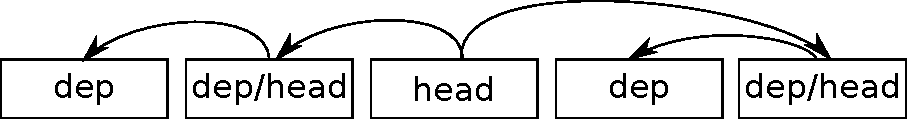
\includegraphics[width=0.9\textwidth]{Figures/SFL-grammar/dependency-dg.pdf}
        \vspace{+22pt}
        \caption{Parent-daughter relations}
        \label{fig:dependecy-dg}
    \end{subfigure}%
    \begin{subfigure}{.5\textwidth}
        \centering
        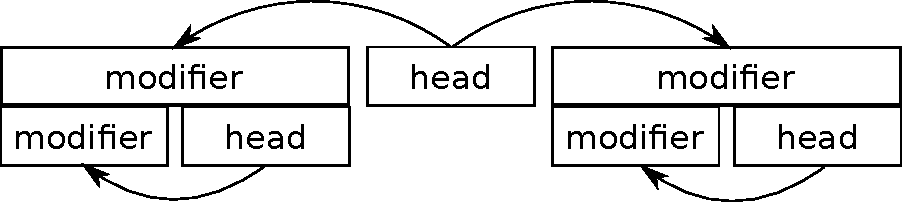
\includegraphics[width=0.9\textwidth]{Figures/SFL-grammar/dependency-sfg.pdf}
        \caption{Sibling head-modifier relations}
        \label{fig:dependecy-sfg}
    \end{subfigure}
    \caption{Plain dependency relations in Dependency and Systemic Functional representation}
    \label{fig:dependency-relations}
\end{figure}

Figure \ref{fig:dependency-relations} illustrates side by side the parent-daughter and sibling dependency relations in a simplified form. In Figure \ref{fig:dependecy-dg} dependencies are the only relations between the units of structure whereas in Figure \ref{fig:dependecy-sfg} are two levels (ranks) of units where the dependency relations are relevant only between sibling elements at the same level within the structure of a unit. As we have seen in Chapter \ref{ch:sfg} knowing only the unit elements is not enough to construct the constituency structure, but it is informative enough for deducing the missing parts. What the Figure \ref{fig:dependency-relations} illustrates is that the two structures resemble each other in a suggestive fashion that will be used below to construct a bridge between descriptions.  

%%%%6. what exactly is the unpacking  principle

The intuitions from the above examples can be laid out by and large in Generalizations \ref{gen:correspondence1}--\ref{gen:correspondence3}. Here I use the term \textit{projection} to refer specifically to the correspondences between theoretical primitives of the two grammars. I say that a primitive in in theory A is projected as another primitive in theory B. The first generalisation is on maximally accounting for the dependency nodes in constituency structure.

\begin{generalization}[Structural Completeness]\label{gen:correspondence1} %maximal accounting
 Each node of the dependency representation is projected, in constituency representation, into one or more units and one or more elements at different rank scales.
\end{generalization}

When translated to a constituency unit, the dependency node, stands for a unit as a whole, the head element of that unit and the word expounding that element. 
For example, the root verb ``seemed'' in a dependency graph corresponds to the clause node and, the Main Verb element and the lexical item which fills the Main Verb of the clause. By analogy, the node ``witness'' stands for the nominal group, the head noun of a Nominal Group and fills the head element of the group.
Even the functional words such as prepositions that in collapsed dependency representation remain orphaned (see Figure \ref{fig:prep-transf2}) have to be accounted in the constituency structure. 

\begin{generalization}[Functional Projection]\label{gen:correspondence2}
    Each dependency relation (alone or contextualised by the word classes of the bridged nodes) is projected into the element of the unit corresponding to the subordinate node. 
\end{generalization}

The dependency relation is primarily responsible for determining the element. For example the ``nsubj'' dependency relation will be projected into a Subject element of a clause unit. Sometimes however, as stated in Generalisation \ref{gen:correspondence2}, the dependency relation alone is not enough and the context given by the governor and subordinate nodes is needed to choose the element. For example the adverbial modifier (advmod) relation alone is not enough to determine into which element to project the subordinate. If the word class context is considered then the verb-to-adverb ``advmod'' relation (VB-advmod-RB) is projected into an Adjunct while the noun-to-adverb ``advmod'' relation (NN-advmod-RB) into is projected Predeictic.  

\begin{generalization}[Substantial Projection]\label{gen:correspondence3}
    Each dependency node projects either the filling or expounding of an element, by a unit of the rank below or by the lexical item of the node. 
\end{generalization}

Generalisation \ref{gen:correspondence3} provides the link between the projected unit with the element of the rank above. For example the subordinate ``witness'' receiving  nominal subject edge from ``seemed'' is responsible for projecting that the Subject element of the clause if filled by the nominal group (headed by the ``witness'' because it is also the governor in the next relation that projects it is the head). The governor ``seemed'', as the root of the tree, is projected into a lexical item which expounds the Main Verb Element (the head of the clause group). In a similar manner, the governor ``witness'' of the determiner (det) relation to ``the'' is projected into a lexical item expounding the Head element (of the nominal group). 

% anotehr example 

\begin{table}[ht]
	\centering
	\begin{tabular}{c|c|c|cc}
        \hline
        \multicolumn{1}{|c|}{\textit{some}}          & \textit{very}   & \textit{small}   & \multicolumn{1}{c|}{\textit{wooden}} & \multicolumn{1}{c|}{\textit{ones}} \\ \hline
        \multicolumn{5}{|c|}{nominal group}                                                                                                                           \\ \hline
        \multicolumn{1}{|c|}{Quantifying Determiner} & \multicolumn{2}{c|}{Epithet}       & \multicolumn{1}{c|}{Classifier}      & \multicolumn{1}{c|}{Head}          \\ \hline
        & \multicolumn{2}{c|}{quality group} &                                      &                                    \\ \cline{2-3}
        & Temperer        & Apex             &                                      &                                    \\ \cline{2-3}
    \end{tabular}
	\caption{SF analysis of Example \ref{ex:small-wooden} (reproduced from Table \ref{tab:example-substructure-analisys-cardiff} )}
	\label{tab:example-substructure-analisys-cardiff-repeated}
\end{table}

\begin{figure}[ht]
	\centering
	\begin{dependency}[dep-style-narrow]
		\begin{deptext}[]
			some/DT \& very/RB \& small/JJ \& wooden/JJ \& ones/NNS \\
		\end{deptext}
		\depedge[edge unit distance =2.2ex]{5}{1}{det}
		\depedge{3}{2}{advmod}
		\depedge{5}{3}{amod}
		\depedge{5}{4}{amod}
	\end{dependency}
	\caption{Dependency analysis for Table \ref{tab:example-substructure-analisys-cardiff-repeated} }
	\label{fig:small-wooden-dependecy}
\end{figure}

%The dependency structure is overloaded with two kinds of meaning

Figure \ref{fig:small-wooden-dependecy} and Table \ref{tab:example-substructure-analisys-cardiff-repeated} represent the analysis of a nominal group from Example \ref{ex:small-wooden} (``some small very small wooden ones'') in the SFG and the Stanford dependency grammar contrasting the two structures. Consider the dependency relation ``det'' acting as a link between the noun ``ones'' and the determiner ``some''. When translated into the SF variant the dependency relation stands within the nominal group between the Head element (filled by word ``ones'') and the Quantifying Determiner element (filled by the word ``some''). As mentioned earlier all the elements in a unit are equal in the structure so the Head and Quantifying Determiner are siblings. So the items (words) filling those elements are also siblings. How then is the dependency relation established? 

% going again on explaining the SFL dependecy

%In SFL there is the concept of Head and Modifier. There is no direct relationship between them, the Modifier and Head stand for two different kinds of meaning and what the Modifier modifies is not the Head per se but the referent denoted by the head (and thus what is construed by the entire unit). It is precisely this modification of the head that is called a (sibling) dependency relation and is seldom mentioned in the SFL literature because it is considered implicit and recoverable from the SF constituency structure.

%strange paragraph, avoid refering to unit anchors
%The Head also is the element that acts as an anchor for the entire unit. In this sense the word ``ones'' realizes not only the Head function (sided with Determiner ``some'') but also anchors the entire unit. The relation between the group and it's elements is one of \textit{componence} (Definition \ref{def:componence}) described in Section \ref{sec:componence}. Yet in the role of unit anchor we cannot say that there is a componence relation between ``one'' and ``some'' because it is merely a proxy to the referent rather than the entire unit. So in this role ``one'' can be said to be standing in a parent-daughter dependency relation to ``some'' incorporating the filling and componence relations.

% example of the relation being unpacked
Lets look at a second example of the two relations ``advmod'' from ``small'' to ``very'' and ``amod'' from ``ones'' to ``small'' in Figure \ref{fig:small-wooden-dependecy}. The interesting case here is the item ``small'' which is the head (Apex) of the quality group. I it anchors the meaning of the whole group and the quality group fills the Modifier/Epithet element within the nominal group. What is not covered in previous example is that the Apex ``small'' not only is a representative of the entire group but it also suitable filler on its own for the Modifier element within nominal group. Using the similar translation mechanism as above, this means that, the incoming dependency needs to be unpacked into three levels: the element within the current group (Modifier), the unit class that element is filling (Quality Group) and finally the head of the filler group (Apex). In fact, to be absolutely correct there is one more level. The elements of a unit are expounded by lexical items, so a fourth relation to unpack is the expounding of the Apex by the word ``small''.

%concluding
I just showed how the dependency relation in dependency structure (Figure \ref{fig:dependecy-dg}) can be unpacked into compounding elements of a unit (Figure \ref{fig:dependecy-sfg}) corresponding to the the sibling dependency considered an indirect relation between the Head and the Modifier (in the Logical metafunction); and then from that using Generalisations \ref{gen:correspondence1}--\ref{gen:correspondence3} deduce the rest of the constituency structure such as the componence relation between unit head and the compounding elements and the filling/expounding relation between the element and the unit right below. 


%do not mention algorithm yet
%TODO[JB] I don't get the impression that we have seen an algorithm yet: just a pointer to the kinds of considerations and differences. So it might help to present a summary which looks more explicitly like an algorithm if you really want to say this here, which would be fine. Do you need to have more information explained before presenting the algorithm? if not, why not put here. If you do, then say very clearly that it will come later, because you don't really mention an algorithm explicitly up to this point. You just say that "the algorithm" will require something... which is not yet very clear.
%In this section I laid the theoretical principle for transforming the dependency structure into systemic functional structure. 

In practice to achieve this level of unpacking two traversals are needed a bottom-up and a top one. This is because the traversal sequence also creates a context that deals with either instantiation a new unit and establishing its elements or with filling an element of a unit above. But more on how to enact the cross theoretical links from this chapter is provided in Section \ref{sec:creation-constituency-graph}.

%TODO [JB] as I mentioned in the previous round of comments, you are going to have to say something more about this. Many many linguists think that null elements are a figment of Chomsky's madness and they are completely unnecessary within a linguistic treatment. So you certainly cannot just assume that they need to be treated. You will have to motivate just why you are going to go this path. You will not be able to prove it is the right path but you should be able to say why it is considered a beneficial or productive kind of solution to your goals in the current thesis.

As motivated elsewhere, I present an account for the unrealised, covert (Null) elements in syntactic structure, using the Governance and Binding Theory. It is also an opportunity to perform a similar cross-theoretical projection exercise.

%
%\todo{close the chapter}
%
%\explain{the problem of bottom up and top down view on the tree structure, due to the fact that head elements plays two roles: of the unit-class(from above) and head-element(from below)}
%\explain{how it is solved with two traversals in the syntactic parsing chapter}
%
%\section{Discussion}
%todo
% \chapter{Government and binding theory}
\label{ch:gbt}


%The rich Systemic Functional constituency structures resulting from the parsing 

Transitivity analysis in SFL is similar to what \textit{semantic role labelling}, \textit{thematic}  or  \textit{$\theta$ role analysis} means in other theories. This thesis provides, in Chapter \ref{ch:semantic-parsing}, an account of how to perform SF Transitivity parsing resulting in a configuration of a process, participants and circumstances. For an illustration take Example \ref{ex:demo-trans1} whose Transitivity analysis is available in Table \ref{tab:demo-trans1}. Here the entire clause is analysed as a Possessive configuration governed by the verb ``receive'' where ``Albert'' plays the \textit{role} of the Affected-Carrier and ``a phone call'' is the thing being Possessed.

\begin{exe}
    \ex\label{ex:demo-trans1} Albert received a phone call.
    \ex\label{ex:demo-trans2} He asked to go home immediately.
%    \ex\label{ex:demo-trans3} He asked [\textit{empty-subject} to go home immediately].
\end{exe}

\begin{table}[!ht]
    \centering
    \begin{tabular}{|c|c|c|c|c|}
        \hline
        \textit{Albert}  & \textit{received} & \textit{a} & \textit{phone} & \textit{call} \\ \hline
        \multicolumn{5}{|c|}{Possessive configuration}                                     \\ \hline
        Affected Carrier & Process           & \multicolumn{3}{c|}{Posessed}               \\ \hline
    \end{tabular}
    \caption{Transitivity analysis with Cardiff grammar of Example \ref{ex:demo-trans1}}
    \label{tab:demo-trans1}
\end{table}

Example \ref{ex:demo-trans2} is slightly more complex and illustrates the main motivation behind the current chapter. It is analysed in Table \ref{tab:demo-trans2}, according to Cardiff grammar, as a Three Role Cognition configuration with ``ask'' being the process, ``he'' the Agent and ``to go home immediately'' the cognised Phenomenon. The Phenomenon is filled by a non-finite clause ``to go home immediately'' which is, in Transitivity account, a Directional configuration governed by the verb ``go'' and has as participants the Destination ``home'' and the Agent Carrier in an empty Subject position that is said to be \textit{non-realised}, \textit{empty}, or \textit{covert}. This is a case when the empty constituent is recoverable from the clause above and corresponds to the Subject ``He''. This way, the constituent ``He'' plays two roles: first as Agent in the Cognition process of the top clause and second as Agent Carrier in the Directional process of the embedded clause. In this work, the way to assign a second role coming from the lower clause, is by detecting and making explicit the empty constituents and resolving them locally with a link to the corresponding constituent.

%TODO: perhaps argue more for the need of having in the structure of something that is not visible; 
%TODO: perhaps use the configuration definitions as an argument, that there are mandatory arguments and optional ones, and sometimes the mandatory ones are not found in the clause and that has to be somehow handled. 

\begin{table}[!ht]
    \centering
    \begin{tabular}{cc|c|c|c|c|c}
        \hline
        \multicolumn{1}{|c|}{\textit{He}} & \textit{asked} & \textit{{[}empty subject{]}} & \textit{to} & \textit{go} & \textit{home} & \multicolumn{1}{c|}{\textit{immediately}} \\ \hline
        \multicolumn{7}{|c|}{Three Role Cognition configuration}                                                                                                                      \\ \hline
        \multicolumn{1}{|c|}{Agent}           & Process        & \multicolumn{5}{c|}{Phenomena}                                                                                       \\ \hline
        &                & \multicolumn{5}{c|}{Directional Configuration}                                                                       \\ \cline{3-7} 
        &                & Agent-Carrier                &             & Process     & Destination   &                                           \\ \cline{3-3} \cline{5-6}
    \end{tabular}
    \caption{Transitivity analysis with Cardiff grammar of Example \ref{ex:demo-trans2}}
    \label{tab:demo-trans2}
\end{table}

In language there are many cases where constituents are empty but recoverable from the immediate vicinity relying in most cases on syntactic means and in a few cases additional lexical-semantic resources are required. The mechanisms of detecting and resolving the empty constituents are captured in the Government and Binding Theory (GBT) developed in \citep{Chomsky81, Chomsky1982, Chomsky1986} and based on the phrase structure grammar. GBT explains how some constituents can \textit{move} from one place to another, where are the places of \textit{non-overt constituents} and what constituents do they refer to i.e. what are their \textit{antecedents}. 

The GBT approach explains grammatical phenomena using \textit{phrase structures} (PS). This is more distant from SFG than the approach taken by the dependency grammar. Section \ref{sec:null-elements-gbt} briefly introduces the theoretical context of GBT and then formulates the principles and generalisations relevant for current work. Then Section \ref{sec:placing-null-elements} translates the introduced principles and generalisations into Dependency Grammar rules and patterns. To lay the ground for the two sections, I first place GBT into the context of transformational grammar and introduce the basic concepts.

\section{Introduction to GBT}
\label{sec:phrase-structure}

This section is set as introduction to the fundamental concepts from Government and Binding Theory. It belongs to the family of Transformational grammars (TG) or transformational-generative grammars (TGG). It is part of the theory of generative grammar that considers grammar to be a system of rules that generate exactly those combinations of words which form grammatical sentences in a given language \citep{Chomsky65}. TG involves the use of defined operations called transformations to produce new sentences from existing ones.

Chomsky developed a formal theory of grammar \citep{Chomsky56} where transformations manipulated not just the surface strings, but the parse tree associated with them, making transformational grammar a system of tree automata \citep{Stockwell1973}.

A transformational-generative (or simply transformational) grammar thus involved two types of productive rules: \textit{phrase structure rules}, such as ``S -> NP VP'' (meaning that a sentence may consist of a noun phrase followed by a verb phrase) etc., which could be used to generate grammatical sentences with associated parse trees (phrase markers, or P markers); and \textit{transformational rules}, such as rules for converting statements to questions or active to passive voice, which acted on the phrase markers to produce further grammatically correct sentences \citep[59-66]{Bach1966}. This notion of transformation proved adequate for subsequent versions including the ``extended'', ``revised extended'' and Government-Binding (GB) versions of generative grammar, but may no longer be sufficient for the latest ``minimalist'' grammar \citep{Chomsky93}. It require a formal definition that goes beyond the tree manipulation. For the purpose of the current work, however, the GBT employing the idea of transformations is perfectly suitable. I selected it because of clear and extensive descriptions of the mechanisms for identification of \textit{null elements} (also known as \textit{empty categories}) and how to provide them with an interpretation. 

\subsection{Phrase structure}
The notion of structure in a generative grammar refers to the way words are combined together to form phrases and sentences. \textit{Merging} is the technical term used in GBT for the operation of bringing two words together into a phrase. In this operation one word will always be more prominent and is therefore called the \textit{head} of the phrase. The resulting combination is a new constituent and is called a \textit{projection} of the head. This is known as \textit{X-bar theory} (often denoted as X' or $\bar{X}$) and embodies two primary claims: (a) that the phrases may contain intermediary constituents projected from a head X and (b) that this system of projected constituency may be common to more than one category (such as N, V, A, P etc.).

These combinations of words and projections can be represented using the \textit{labelled bracketing notation} where the labels denote constituent categories. The bracketed notation is a representation equivalent to a hierarchical tree of constituent parts or \textit{parse tree} (also known as \textit{syntactic tree}, \textit{phrase structure}, \textit{derivation tree}). The parse tree represents the syntactic structure of a string according to some grammar. The equivalence between a bracketed notation and parse tree is exemplified in the following two representations of \ref{ex:example-sent} from \citep[83]{Haegeman1991}.

\begin{exe}
    \ex\label{ex:example-sent} Poirot will abandon the investigation.
    \ex\label{ex:bracketed}
    $
    \Bigg[_S
    \Big[_{NP}
    \big[_NPoirot\big]
    \Big]
    \big[_{AUX}will\big]
    \bigg[_{VP}
    \big[_Vabandon\big]
    \Big[_{NP}
    \big[_{Det}the\big]
    \big[_Ninvestigation\big]
    \Big]
    \bigg]
    \Bigg]
    $
\end{exe}

\begin{figure}[!ht]
    \centering
    \Tree [.S [.NP [.N Poirot ] ] [.AUX will ] [.VP [.V abandon ] [.NP [.Det the ] [.N investigation ]]]]
    \caption{The parse tree of Example \ref{ex:example-sent} from \citep[83]{Haegeman1991} }
    \label{fig:exaple-parse-tree}
\end{figure}

A node is said to be \textit{non-branching} if there is a single line starting below and it is called  \textit{branching} if there are more than one line going downwards. The children of a branching node are said to be bound by a \textit{sisterhood} relation and in relation to a \textit{parent} or \textit{mother} node. In a phrase structure the vertical relations are referred as \textit{dominance} relations defined below. 

\begin{definition}[Dominance]\label{def:dominance}
    Node A dominates node B if and only if A is higher up in the tree than B and if you can trace a line from A to B going only downwards \citep[85]{Haegeman1991}.
\end{definition}

Looking at the tree diagram along the horizontal axis, GBT describes left-to-right ordering of constituents using the \textit{precedence} relation. 

\begin{definition}[Precedence]\label{def:predecence}
    Node A precedes node B if and only if A is to the left of B and neither A dominates B nor B dominates A \citep[85]{Haegeman1991}.
\end{definition}

In Figure \ref{fig:exaple-parse-tree} NP, AUX and VP nodes are sisters, they precede each other and are dominated by S parent node. A more specific type of dominance, that will be employed latter in this chapter, is the \textit{immediate dominance} which is when there is no intermediary node between A and B. In this case, the node ``Poirot'' is also dominated by S but only the grandparent NP is immediately dominated by S. 
The same holds for precedence: the \textit{immediate precedence} is when a node A precedes a node B and there is no intervening node in between. Node NP precedes VP but only AUX is immediately preceded. 

\begin{generalization}[Projection principle]\label{gen:pp}
    Lexical information is syntactically represented. 
\end{generalization}

\begin{figure}[!ht]
    \centering
    \Tree [.S  
            [.NP {Miss Marple} ] 
            [.AUX will ] 
            [.VP 
                [.$\bar{V}$ 
                    [.$\bar{V}$  
                        [.V read ] 
                        [.NP {the letters} ] 
                    ]  
                    [.PP {in the garden shed} ] 
                ] 
                [.NP {this afternoon} ] 
            ] 
        ]
%    \Tree [.VP [.V read ] [.NP {Miss Marple} ] ]
    \caption{Example of projections from \citep[90]{Haegeman1991} }
    \label{fig:maximal-projection}
\end{figure}

An important principle in GBT is that of \textit{projection} formulated in Generalisation \ref{gen:pp}. For example in Figure \ref{fig:maximal-projection}, projections of V that are dominated by more comprehensive projections of V are called \textit{intermediate projections} while the node labelled VP is the \textit{maximal projection} of V. Maximal projections are also barrier to government (see Definition \ref{def:government1} below). The role of lexicon in syntax from to GBT perspective is discussed at large in \citet{stowell1992syntax}. 

\subsection{Theta theory}
This section introduces which constituents are minimally required to form a sentence and why. Traditionally three types of verbs are recognised: \textit{transitive}, \textit{di-transitive} and \textit{intransitive}. This distinction is based on how many complements a verb requires to form a minimal complete sentence. If a verb is transitive then one NP direct object is required. If the verb is di-transitive then two NP or one NP and one PP direct and indirect objects are required. Finally, if it is intransitive then no NP complement is allowed. 

Logicians for a long time have been concerned with formulating representations corresponding to semantic structure of sentences or \textit{propositions}. Like Tesniere \citep[97]{Tesniere2015} discussed in Section \ref{sec:origins}, Haegeman employs the metaphor of a theatre play when discussing the argument structure of predicates. A play not only describes the number of participants but also what corresponding roles they play. The specific semantic relations between the verb and its arguments is comparable with the identification of characters in a play script \citep[49]{Haegeman1991}.
 
In logical notation such as in Example \ref{ex:argument} a proposition comprises of a predicate (P) that takes a certain number of \textit{arguments} (here a and b). By analogy to the logical tradition, in GBT, the verb is said to be like the predicate while the Subject together with complements are like the arguments that the predicate requires. 

In Example \ref{ex:kill1} Maigret, taking Subject position, is the Agent in the process of killing while Poirot in the complement position is the Patient that receives the effects of the process of killing. The generic argument structure for the verb ``to kill'' can be expressed as in Example \ref{ex:kill2}. The first argument is of NP category and takes the role of an Agent while the second argument is also an NP but it takes the Patient role. The transitivity of a verb dictates how many arguments there should be.

\begin{exe}
    \ex\label{ex:argument} P(a, b)
    \ex\label{ex:kill1} Maigret killed Poirot.
    \ex\label{ex:kill2} V kill: 1 (NP:Agent), 2 (NP:Patient)
\end{exe}

In literature these relations between the verb and the arguments are called \textit{thematic roles} or theta-roles ($\theta$-roles). It is said that the verb \textit{theta marks} its arguments. The component of the grammar that regulates the assignment of thematic roles is called \textit{theta theory}. 

In GBT the theory of thematic roles is very sketchy and does not go beyond distinction of several thematic roles (Agent/Actor, Patient, Theme, Experiencer, Beneficiary, Goal, Source, Location and the controversial Theme) \citep[50]{Haegeman1991}. The theta theory has a central criterion that is stipulated in Generalisation \ref{gen:theta-criterion}.

\begin{generalization}[Theta criterion]\label{gen:theta-criterion}
    Theta criterion requires that: 
    \begin{itemize}
        \item each argument is associated one and only one theta role
        \item each theta role is assigned to one and only one argument \citep[54]{Haegeman1991}
    \end{itemize} 
\end{generalization}

\begin{exe}
    \ex\label{ex:expletive1} \textit{It} surprised Jeeves that the pig had been stolen.
\end{exe}

In English, however, there is a special case, that of \textit{expletives}, when the Subject argument is filled by the pronoun \textit{it} that receives no thematic role and acts rather as a dummy slot filler without any semantic contribution to the meaning of the sentence \citep[62]{Haegeman1991}. Worth noticing is also the fact that \textit{auxiliary verbs} and \textit{copula verbs} do not assign thematic roles \citep{pollock1989verb}. 

The verb that assigns a theta role does not need to specify which syntactic category it shall be realised by. In more technical it means that the categorial selection (\textit{c-selection}) follows from semantic relation (\textit{s-selection}). When a theta role can be assigned to an argument it is said that it is saturated. In order to identify the assignment of respective role the arguments are identified by the means of an index provided as subscript in the sentence. 

\begin{exe}
    \ex\label{ex:indexing1} Maigret_i killed the burglar_j.
    \ex\label{ex:indexing2} Maigret_i said that he_i was ill.
\end{exe}

In the Example \ref{ex:indexing1} Maigret has the index \textit{i} and the burglar \textit{j} meaning they are distinct referents. On contrary, in Example \ref{ex:indexing2}, ``he'' receives the same index as Maigret because they are interpreted as referring to the same entity. We say that the two are \textit{coindexed}.

%This is a sufficient foundation for introducing next the \textit{government theory}.
\subsection{Government and Binding}
%Government is a structural property involved in syntactic processes such as theta-marking \ref{} and case-marking \ref{} that is introduced below.

Using the terminology from the traditional grammar it is said that a verb governs its object. This is generalised in GBT as a rule that the head of a phrase, called \textit{governor}, \textit{governs} its complement, called the \textit{governee}. This relation is loosely defined in Definition \ref{def:government-i} below and formally in Definition \ref{def:government1}. 

\begin{definition}[government i]\label{def:government-i}
     A governs B if 
     \begin{itemize}
         \item A is a governor;
         \item A and B are sisters
     \end{itemize}
     Governors are heads \citep[86]{Haegeman1991}.
\end{definition}

In Figure \ref{fig:exaple-parse-tree} the verb ``abandon'' is the head of the verb phrase (VP) and governs the direct object - nominal phrase (NP) ``the investigation''. V does not govern the subject NP ``Poirot''. All the constituents governed by a node constitute the \textit{governing domain} of that node. In this case VP is the governing domain of V.

Before providing the next definition of government, I first introduce the notion of C-command which provides a general pattern of how the agreeing elements relate to each other in the parse tree. C-command is formally defined in Definition \ref{def:c-command}. When considering the geometrical relation between the agreeing elements, one always is higher in the tree than the other one in a manner depicted in Figure \ref{fig:agreement2}. In Figure \ref{fig:agreement1} the co-subscripted nodes indicate agreement. Here the [Spec, NP] c-commands all the nodes dominated by the NP. These nodes constitute the \textit{c-command domain} of Spec element \citep[134]{Haegeman1991}. 

\begin{figure}[!ht]
    \centering
    \begin{subfigure}{0.45\linewidth}
        \centering
        \Tree [.NP [.Spec_i le ] [.$\bar{N}$ [.N_i livre ] [.PP sur Chomsky ]]]
        \caption{Example of agreement in French \citep[132]{Haegeman1991} }
        \label{fig:agreement1}
    \end{subfigure}
    \begin{subfigure}{0.45\linewidth}
     \centering
    \Tree [.X [.A_i ] [.{\ldots} [.B_i ] {\ldots} ]]
    \caption{Schematic representation of the c-command \citep[133]{Haegeman1991} }
    \label{fig:agreement2}
\end{subfigure}
    \caption{Agreement example and schematic representation }
    \label{fig:agreement}
\end{figure}

\begin{definition}[c-command]\label{def:c-command}
    A node A c-commands a node B if and only if
    \begin{itemize}
        \item A does not dominate B;
        \item B does not dominate A;
        \item the first branching node dominating A also dominates B \citep[212]{Haegeman1991}.
    \end{itemize}
\end{definition}

\begin{definition}[Government]\label{def:government1}
    X governs Y if and only if
    \begin{itemize}
        \item X is either of the category A, N, V, P, I; \\
            or \\
            X and Y are coindexed
        \item X c-commands Y;
        \item no barrier intervenes between X and Y;
        \item there is no Z such that Z satisfies the points above and X c-commands Z \citep[557]{Haegeman1991}.
    \end{itemize}
\end{definition}

%After having introduced government I turn next to the binding theory. 
%np definitions
IN GBT three types of NP are distinguished: \textit{full noun phrases} (e.g. Maigret, the doctor,  etc.), \textit{pronouns} (e.g. he, me, us, etc.), and \textit{anaphors} comprised of reflexives (e.g. myself, herself, etc.) plus reciprocals (e.g. each other, one another,). 
Pronouns and anaphors (reflexives and referential) lack inherent reference. Anaphors need an antecedent for their interpretations whereas pronouns do not. Pronoun indicate some inherent features of the referent so that they can be identified from the contextual information. The full noun phrases called Referential expressions or \textit{R-expression}, for short, are inherently referential and do not need an antecedent, moreover they do not tolerate an antecedent \citep[226]{Haegeman1991}. The NP types can be defined in terms of features Anaphor and Pronominal (systematised together with the empty categories in the Table \ref{tab:null-types} below). This way the Pronouns have features [+Pronominal,-Anaphor], the Anaphors [+Pronominal,-Anaphor] and the R-expressions [-Pronominal,-Anaphor]. The last combination [+Pronominal,+Anaphor] corresponds to \textit{PRO empty category} which will be discussed in the Section \ref{sec:pro-mcg} coming up next. 

The module of the grammar regulating interpretation of the noun phrase (NP) interpretation is referred, in GBT, as the \textit{binding theory}. It is formally defined in terms of c-command in Definition \ref{def:binding}. And because the BT is essentially concerned with binding of NPs in argument positions (\textit{A-position}) then it is rather the \textbf{A-binding} (see Definition \ref{def:a-binding}) of interest here. An A-position is a position in the tree to which a theta role can (but not necessarily) be assigned \citep[115]{Haegeman1991}.

\begin{definition}[Binding]\label{def:binding}
    A binds B if and only if
    \begin{itemize}
        \item A c-commands B;
        \item A and B are coindexed \citep[212]{Haegeman1991}.
    \end{itemize}
\end{definition}

\begin{definition}[A-Binding]\label{def:a-binding}
    A A-binds B if and only if
    \begin{itemize}
        \item A is in A-position;
        \item A c-commands B;
        \item A and B are coindexed \citep[240]{Haegeman1991}.
    \end{itemize}
\end{definition}

Each of these NP types have an associated binding principle (ways in which to interpret, if needed, the reference of the NP) provided in Generalisations \ref{gen:binding-theory-a}, \ref{gen:binding-theory-b} and \ref{gen:binding-theory-c} below. These principle use the idea of \textit{governing category} which for a node A is the minimal domain containing it, its governor and an accessible subject. A subject A is said to be accessible for B if the co-indexation of A and B does not violate any grammatical principle \citep[241]{Haegeman1991}.

\begin{generalization}[Principle A of binding theory]\label{gen:binding-theory-a}
    An anaphor (i.e. a NP with the feature [+Anaphor] covering reflexives and reciprocals) must be bound in its governing category \citep[224]{Haegeman1991}.
\end{generalization}

\begin{generalization}[Principle B of binding theory]\label{gen:binding-theory-b}
    The pronoun (i.e. a NP with feature [+Pronominal]) must be free in its governing category \citep[225]{Haegeman1991}.
\end{generalization}

\begin{generalization}[Principle C of binding theory]\label{gen:binding-theory-c}
    An R-expression (i.e. a NP with independent reference) must be free everywhere \citep[227]{Haegeman1991}.
\end{generalization}


\section{On Null Elements}
\label{sec:null-elements-gbt}
In certain schools of linguistics, in the study of syntax, an \textit{empty category} is a nominal element that does not have any phonological content and is therefore unpronounced. Empty categories may also be referred to as \textit{covert nouns}, in contrast to overt nouns which are pronounced \citep{Chomsky1993lectures}. Some empty categories are governed by the \textit{empty category principle} (see Definition \ref{def:ecp}). When representing empty categories in trees, linguists use a null symbol to depict the idea that there is a mental category at the level being represented, even if the word(s) are being left out of overt speech. 
%GBT recognizes four main types of empty categories: NP-trace, Wh-trace, PRO, and pro.

GBT recognises four main types of empty categories: \textit{NP-trace}, \textit{WH-trace}, \textit{PRO}, and \textit{pro}. They are subject to Principles A, B and C of the binding theory provided above and differentiated, like the over NPs, by two binding features: the anaphoric feature [a] and the pronominal feature [p]. The four possible combinations of plus (+) or minus (-) values for these features yield four types of empty categories. 

\begin{table}[!ht]
	\centering
	%\resizebox{\textwidth}{!h}{%
		\begin{tabulary}{\linewidth}{|c|c|c|C|C|}
			\hline
			\textbf{{[}a{]}} & \textbf{{[}p{]}} & \textbf{Symbol} & \textbf{Name of the empty category} & \textbf{Corresponding overt NP type} \\ \hline
			-                & -                & t               & WH-trace                        & R-expression                           \\ \hline
			-                & +                & pro             & little Pro                      & pronoun                                \\ \hline
			+                & -                & t               & NP-trace                        & anaphor                                \\ \hline
			+                & +                & PRO             & big Pro                         & none                                   \\ \hline
		\end{tabulary}%
	%}
	\caption{Four types of empty categories 
%        according to their binding features 
(adaptation from \citep[436]{Haegeman1991})}
	\label{tab:null-types}
\end{table}

In Table \ref{tab:null-types}, [+a] refers to the anaphoric feature, meaning that the particular element must be bound within its governing category whereas [+p] refers to the pronominal feature which shows that the empty category is taking the place of an overt pronoun.

%todo, is this definition well positioned here? 

\begin{definition}[Empty Category Principle (ECP)]\label{def:ecp}
    % solution taken from https://tex.stackexchange.com/questions/307141/itemizing-theorem-body
    \leavevmode
    \makeatletter
    \@nobreaktrue
    \makeatother
    %    
    \begin{itemize}
        \item Traces must eb properly governed.
        \item A properly governs B if and only if A theta-governs B or A antecedent-governs B \citep[17]{Chomsky1986}.
        \item A theta-governs B if and only if  A governs B and A theta-marks B.
        \item A antecedent-governs B if and only if A governs B and A is coindexed with B \citep[442]{Haegeman1991}.
    \end{itemize}
\end{definition}

%todo some more dineitions mby?


Next I describe in detail each empty category and the properties of corresponding overt noun type. 


\subsection{PRO Subjects and control theory}
\label{sec:pro-mcg}
\textit{PRO} stands for the non-overt NP that is the subject in non-finite (complement, adjunct or subject) clause and is accounted by the \textit{control theory} (CT).

\begin{definition}[Control]\label{def:control}
	Control is a term used to refer to a relation of referential dependency between an unexpressed subject (the control element) and an expressed or unexpressed constituent (controller). The referential properties of the controlled element are determined by those of the controller \citep{Bresnan1982}.
\end{definition}

Control can be \textit{optional} or \textit{obligatory}. While \textit{Obligatory control} has a single interpretation, that of PRO being bound to its controller, the \textit{optional control} allows for two interpretations: \textit{bound} or \textit{free}. In Example \ref{ex:pro4} the PRO is controlled, thus bound, by the subject ``John'' of the matrix clause (i.e. higher clause) whereas in \ref{ex:pro5} it is an arbitrary interpretation where PRO refers to ``oneself'' or ``himself''. In \ref{ex:pro6} and \ref{ex:pro7} PRO must be controlled by the subject of the higher clause and does not allow for the arbitrary interpretation.

\begin{exe}
	\ex\label{ex:pro4}John asked how [PRO to behave himself/oneself].
	\ex\label{ex:pro5}John and Bill discussed [PRO behaving oneself/themselves in public].
	\ex\label{ex:pro6}John tried [PRO to behave himself/*oneself].
	\ex\label{ex:pro7}John told Mary [PRO to behave herself/*himself/*oneself].
\end{exe}

Sometimes the controller is the subject (as in Examples \ref{ex:pro4}, \ref{ex:pro5}, \ref{ex:pro6}) and sometimes it is the object (Example \ref{ex:pro7}) of the higher clause. \citet[278]{Haegeman1991} proposes that there are two types of verbs, verbs of \textit{subject} and of \textit{object control}. The following set of generalizations from \cite{Haegeman1991} are instrumental in identifying places where a PRO constituent can be said to occur and identifies its corresponding binding element.

\begin{generalization}\label{gen:1}
	Each clause has a subject. If a clause doesn't have an overt subject then it is covertly (non-overtly) represented as PRO
     \citep[263]{Haegeman1991}.
\end{generalization}
\begin{generalization}\label{gen:2}
	A PRO subject can be bound, i.e. it takes a specific referent or can be arbitrary (equivalent to pronoun ``one'') \citep[263]{Haegeman1991}. In case of obligatory control, a PRO subject is bound to a NP and must be c-commanded by its controller \citep[278]{Haegeman1991}.
\end{generalization}

\begin{generalization}\label{gen:3}
	PRO must be in ungoverned position. This means that (a) PRO does not occur in object position (b) PRO cannot be subject of a finite clause \citep[279]{Haegeman1991}. 
\end{generalization}
\begin{generalization}\label{gen:4}
	PRO does not occur in the non-finite clauses introduced by \textit{if} and \textit{for} complementizers, but it can occur in those introduced by \textit{whether} \citep[279]{Haegeman1991}.  
\end{generalization}
Examples \ref{ex:pro8} and \ref{ex:pro9} illustrate Generalisation \ref{gen:4}
\begin{exe}
	\ex\label{ex:pro8} John doesn't know [whether [PRO to leave].
	\ex\label{ex:pro9} * John doesn’t know [if PRO to leave].
\end{exe}

\begin{generalization}\label{gen:5}
	PRO can be subject of complement, subject and adjunct clauses \citep[278]{Haegeman1991}.
\end{generalization}
\begin{generalization}\label{gen:6}
	When PRO is the subject of a declarative complement clause it must be controlled by an NP, i.e. arbitrary interpretation is excluded \citep[280]{Haegeman1991}.
\end{generalization}
\begin{generalization}\label{gen:7}
	The object of active clause becomes subject when it is passivized and also controls the PRO element in complement clause \citep[281]{Haegeman1991}.
\end{generalization}
\begin{generalization}\label{gen:8}
	PRO is obligatorily controlled in adjunct clauses that are not introduced by a marker \citep[283]{Haegeman1991}.
\end{generalization}

Adjuncts (clauses or phrases) often are introduced via prepositions. Nonetheless there are rare cases of adjunct clauses free of preposition. Examples \ref{ex:pro10} and \ref{ex:pro11} illustrate such marker-free adjunct clauses.

\begin{exe}
	\ex\label{ex:pro10} John hired Mary [PRO to fire Bill].
	\ex\label{ex:pro11} John abandoned the investigation [PRO to save money].
\end{exe}

\begin{generalization}\label{gen:9}
	PRO in a subject clause is optionally controlled; thus by default it takes arbitrary interpretation \citep[283]{Haegeman1991}.  
\end{generalization}

\begin{exe}
    \ex\label{ex:pro12} PRO_i smoking is bad for the health_j.
    \ex\label{ex:pro13} PRO_i smoking is bad for your_i health_j.
    \ex\label{ex:pro14} PRO_i smoking is bad for you_i.
    \ex\label{ex:pro15} PRO_i lying to your_i friends decreases your_i trustworthiness_j.
\end{exe}

A default assumption is to assign arbitrary ``one'' interpretation to each PRO subject in subject clauses. However, there are cases when it may be bound (resolved) to a pronominal NP in the complement of the higher clause. The binding element can be either the entire complement or a \textit{pronominal} part of it like the qualifier or the possessor. Example \ref{ex:pro12} illustrates that PRO has only arbitrary interpretation since it cannot be bound to the complement ``health''. 
Moreover PRO can also be bound to (a) the possessive element of a higher clause - example \ref{ex:pro13}, (b) the complement of the higher clause - example \ref{ex:pro14} and (c) either the possessives in lower or higher clause, Example \ref{ex:pro15}.

\subsection{NP-traces} 
\label{sec:np-gbt}

In GBT, \textit{movement} is a kind of transformation used to explain discontinuity or displacement phenomena in language. It is based on the idea that some constituents appear to have been displaced from the position where they receive important features of interpretation. 

GBT distinguishes three types of movement: (a) \textit{head-movement} - the movement of auxiliaries from I to C , \textit{Wh-movement} - when the wh-constituent lands in Spec position of a CP (i.e. [Spec, CP]) and (c) NP-movement when a NP is moved into an empty subject position. 
NP-movement in GB theory is used to explain \textit{passivization}, \textit{subject movement} (in interrogatives) and \textit{raising}. The raising phenomenon (Definition \ref{def:raising}) is the one that is of interest for us here as it is the one involving an empty constituent. 

When an NP moves it is said to leave \textit{traces} (Definition \ref{def:trace}). The moved constituent is called \textit{antecedent} of a trace. Both the trace(s) and the antecedent are coindexed and form what is called a \textit{chain} \citep[309]{Haegeman1991}.
 

\begin{definition}[Trace]\label{def:trace}
    A trace is an empty category which encodes the base position of a moved constituent and is indicated as \textit{t} \citep[309]{Haegeman1991}. 
\end{definition}

\begin{definition}[NP-raising]\label{def:raising}
	NP-raising is the NP-movement of a subject of a lower clause into subject position of a higher clause \citep[306]{Haegeman1991}. 
\end{definition}

Consider Examples \ref{ex:np1} to \ref{ex:np4} where I used square brackets to indicate boundaries of an embedded clause. There are two cases of expletives (\ref{ex:np1} and \ref{ex:np3}) and their non-expletive counterparts (\ref{ex:np2} and \ref{ex:np4}) where the subject of the lower clause is moved to the subject position of the matrix clause by replacing the expletive. The movement of NPs are described in GB as leaving traces which here are marked as \textit{t}. This phenomena is called \textit{raising} (Definition \ref{def:raising}) or as \citet{Postal1974} calls it the \textit{subject-to-subject raising}.

\begin{exe}
	\ex\label{ex:np1} It was believed [Poirot to have destroyed the evidence].
	\ex\label{ex:np2} Poirot_{i} was believed [t_{i} to have destroyed the evidence].
	\ex\label{ex:np3} It seems [that Poirot has destroyed the evidence].
	\ex\label{ex:np4} Poirot_{i} seems [t_{i} to have destroyed the evidence].
\end{exe}

The subjects ``It'' and ``Poirot'' in none of the examples \ref{ex:np1}--\ref{ex:np4} receive a semantic role from the main clause. ``It'' is an expletive and never receives a thematic role while ``Poirot'' in \ref{ex:np2} and \ref{ex:np4} takes an Agent role from ``destroy'' and is not the Experiencer neither of ``believe'' nor of ``seem''. So verbs ``believe'' and ``seem'' do not theta mark their subjects in these examples.

Raising is very similar to obligatory subject control with a difference in thematic role distribution. In the case of subject control, both the PRO element and it's binder (the subject of higher clause) receive thematic roles in both clauses. However in the case of raising, the NP is moved and it leaves a trace which is theta marked but not to the antecedent \citep[314]{Haegeman1991}. This is expressed in generalization \ref{gen:np1}. 

\begin{generalization}\label{gen:np1} 
	The landing site for a moved NP is an empty A-position. The chain formed by a NP-movement is assigned only one theta role and it is assigned on the foot of the chain, i.e. the lowest trace \citep[314]{Haegeman1991}.
\end{generalization} 

So, in case of raising, the landing sites for a moved NP are empty subject positions or the ones for expletives. As a result of movement, these positions are filled or expletives are replaced with the moved NP. The last type of movement is the one of NPs that have a \textit{Wh-word} described in the next section.

\subsection{WH-traces}
\label{sec:wh-gbt}
\textit{Wh-movement} is involved in formation of Wh-interrogatives and in formulation of relative clauses. We are interested in both cases as both of them leave traces of empty elements that are relevant for transitivity analysis.  

\begin{exe}
	\ex\label{ex:wh1} [What] will Poirot eat?
	\ex\label{ex:wh2} [Which detective] will Lord Emsworth invite?
	\ex\label{ex:wh3} [Whose pigs] must Wooster feed?
	\ex\label{ex:wh4} [When] will detective arrive at the castle?
	\ex\label{ex:wh5} [In which folder] does Margaret keep the letter?
	\ex\label{ex:wh6} [How] will Jeeves feed the pigs? 
	\ex\label{ex:wh7} [How big] will the reward be?
\end{exe}

\citet[375]{Haegeman1991} offers the Examples \ref{ex:wh1} -- \ref{ex:wh7} of \textit{Wh-constituents} which are any NPs or PPs that contain a \textit{Wh-word} in their componence. A Wh-word is any of the following words or their morphological derivations (by adding suffixes \textit{-ever}, \textit{-soever}): \textit{who, whom, whose, what, which, why, where, when} and \textit{how}. Thus the wh-constituent can be a single word or a \textit{Wh-phrase}. The Wh-phrase, in GBT, is then the NP or PP which is the maximal projection from a Wh-word. Haegeman treats each Wh-word as the head of the Wh-phrase. This is not quite the case . Below, in Section \ref{sec:wh-traces}, I provide a different definition of Wh-group such that it is congruent with the Systemic Functional Grammars.

In GBT the \textit{case} occupies an important place in the grammar. The rules governing the case are known as \textit{case theory}. Verbs dictate the case of their arguments, a property called \textit{case marking}. The Subjects are marked with Nominative case while the Complements of the verb are marked with Accusative case. 

In English, however, case system is very rudimentary as compared to other languages. Hence, \textit{who}, \textit{whom} and their derivatives \textit{whoever} and \textit{whomever} are the only Wh-words with overt case differentiation. The other Wh-words \textit{what, when, where} and \textit{how} do not change their form based on the case. 

Example \ref{ex:wh30} shows that the Accusative (\textit{whom}) is disallowed when its trace is in Subject position since this requires Nominative (\textit{who}). In example \ref{ex:wh31} the reverse holds and the Nominative form is disallowed as the Wh-word moved from Complement position requires Accusative case. 

\begin{exe}
	\ex\label{ex:wh30} Who_{i}/*Whom_{i} do you think [t_{i} will arrive first?]
	\ex\label{ex:wh31} Whom_{i}/*Who_{i} do you think [Lord Emsworth will invite t_{i}?]
\end{exe}

Another important distinction to be made among English Wh-words is the \textit{theta-marking}, i.e. the argument and non-argument distinction. Some wh-constituents will be in A-positions (i.e. functioning as subject or complement) such as in Example \ref{ex:wh1} -- \ref{ex:wh3} or in non A-position (i.e. functioning as adjunct) such as in Example \ref{ex:w4} and \ref{ex:wh6}. 

When the Wh-constituent moves, There are two places where it can land: (a) either in the subject position of the matrix clause changing its mood to interrogative (example \ref{ex:wh8}) or (b) subject position of the embedded clause creating embedded questions (example \ref{ex:wh9}). However regardless of the landing site, the movement principle is subject to what Haegeman describes as \textit{that-trace filter} expressed in Generalisation \ref{gen:wh1} and the \textit{Subjacency condition} (Generalisation \ref{gen:wh2}). Note that the matrix or embedded clauses correspond to the category of inflectional phrase (IP).

\begin{exe}
\ex\label{ex:wh8} Whom_{i} do [you believe [that Lord Emsworth will invite t_{i}]]?
\ex\label{ex:wh9} I wonder [whom_{i} you believe [that Lord Emsworth will invite t_{i}]].
\end{exe}

\begin{generalization}[That-trace filter]\label{gen:wh1}
	The sequence of an overt complementizer ``that'' followed by a trace is ungrammatical \citep[399]{Haegeman1991}.
\end{generalization}

The examples in \ref{ex:wh10} to \ref{ex:wh13} provided by \citet[398]{Haegeman1991} illustrate how the above generalization applies. 
\begin{exe}
	\ex\label{ex:wh10} * Whom do you think that Lord Emsworth will invite?
	\ex\label{ex:wh11} Whom do you think Lord Emsworth will invite?
	\ex\label{ex:wh12} * Who do you think that will arrive first?
	\ex\label{ex:wh13} Who do you think will arrive first?
\end{exe}

\begin{generalization}[Subjacency condition]\label{gen:wh2}
	Movement cannot cross more than one bounding node, where bounding nodes are IP and NP \citep[402]{Haegeman1991}.
\end{generalization}

The Subjacency condition captures the grammaticality of NP-movement and exposes two properties of the movement, namely as being \textit{successive} and \textit{cyclic}. Consider the chain creation resulting from Wh-movement in Examples \ref{ex:wh14} -- \ref{ex:wh16} provided by \citet[403--406]{Haegeman1991}. The Wh-movement leaves (intermediate) traces successively jumping each bounding node. 

\begin{exe}
	\ex\label{ex:wh14} Who_{i} did [he see t_{i} last week?]
	\ex\label{ex:wh15} Who_{i} did [Poirot claim [t_{i} that he saw t_{i} last week?]]
	\ex\label{ex:wh16} Who_{i} did [Poirot say [t_{i} that he thinks [t_{i} he saw t_{i} last week?]]]
\end{exe}

What Generalisation \ref{gen:wh2} states is that a Wh-constituent cannot move further than subject position of the clause forming an interrogative form. Or also it can move outside into the subject position of the clause higher above leaving a WH-trace as can be seen in the Example \ref{ex:wh15} and \ref{ex:wh16}.

Now that the kinds of null elements have been concisely described laying out the main rules governing their behaviour, I turn next to discuss what how these elements can be identified in terms of Dependency grammar. 

\section{Placing Null Elements into the Stanford dependency grammar}
\label{sec:placing-null-elements}
%todo[jb] It would be worthwhile to consider moving this to the short chapter which describes overall system architecture which should follow (see email). This would be the cleanest place for doing the integration first at a theoretical level, drawing connections, and then implementationally, in terms of a system architecture. 

This section provides a selective translation of principles, rules and generalisations captured in GB theory into the context of dependency grammar. The selections mainly address the identification of places where (and by which relations) the null elements should be injected into dependency structure that will later help the semantic parsing process described in Chapter \ref{ch:semantic-parsing}. 

In this section the grammatical accounts will often overlap. To make a clear distinction I will mark the dependency grammar relations with small caps italic. When the syntactic functions are marked with capital letter (e.g. Subject, Complement, Deictic) then they mean SFG functions and if they are in lower case (e.g. direct and indirect object) then the GBT reading applies. When the (unit/word) classes are mentioned using full word small caps (nominal group, clause, ) then the SFL reading shall be applied and when they are all caps acronyms (NN, PP, WH-trace, etc.) the reader shall apply GBT reading .

\subsection{PRO subject}
% % % % % % % % % % % % % % % % % % % % % % % %
Coming back to definition of PRO element in Section \ref{sec:pro-mcg}, it is strictly framed by the non-finite subordinate clauses. In dependency grammar the non-finite complement clauses are typically linked to their parent via \textit{xcomp} relation which is defined in \cite{Marneffe2008} as introducing an open clausal complement of a VP or ADJP without its own subject, whose reference is determined by an external reference as can be seen in Figure \ref{fig:xcomp-ex}.

%%todo , interrogatives with we element in embedded clause have PRO subjects
%ex:pro4
%John decided to behave himself.
%ex:pro7
%John told Mary to behave herself.

\begin{figure}[!ht]
    \centering
    \begin{subfigure}[t]{0.45\linewidth}
%        \centering
%        \scalebox{1}{
        \begin{dependency}[dep-style]
            \begin{deptext}[]
                John_i \& decided \& PRO_i \& to \& behave.\\
            \end{deptext}
            \deproot{2}{root}
            \depedge{2}{1}{nsubj}
            \depedge{2}{5}{xcomp}
            \depedge{5}{3}{nsubj}
            \depedge{5}{4}{mark}
        \end{dependency}
%    }
        \caption{}
        \label{fig:xcomp-ex1}
    \end{subfigure}

    \begin{subfigure}[t]{0.45\linewidth}
%        \centering
%        \scalebox{1}{
        \begin{dependency}[dep-style]
            \begin{deptext}[]
                John_i \& told \& Mary_j \& PRO_j \& to \& behave \& herself_j. \\
            \end{deptext}
            \deproot{2}{root}
            \depedge{2}{1}{nsubj}
            \depedge{2}{6}{xcomp}
            \depedge{2}{3}{dobj}
            \depedge{6}{4}{nsubj}
            \depedge{6}{5}{mark}
            \depedge{6}{7}{dobj}
        \end{dependency}
%    }
        \caption{}
        \label{fig:xcomp-ex2}
    \end{subfigure}
    \caption{Dependency structure with a PRO subject}
    \label{fig:xcomp-ex}
\end{figure}

These complements are always non-finite. Following the principles stated in Generalisation \ref{gen:1} and \ref{gen:3} the non-finite complement clause introduced by \textit{xcomp} relation would receive by default a PRO subject (controlled or arbitrary).

The markers (conjunctions, prepositions or Wh-words) at the beginning of the embedded clause are no longer connected via \textit{xcomp} relation but instead via either \textit{prepc}, \textit{rcmod}, \textit{partmod} and \textit{infmod} and a slight variation in clause features and constituency. Those cases are no longer treated under the PRO null element considerations and will be discussed later in this chapter since they correspond to other types of empty elements. The only exception, however, is the \textit{prepc} relation only with the preposition ``whether'' which also introduces a complement clause with PRO element.

%\begin{figure}[H]
%	\centering
%	\begin{tikzpicture}[tree-style] 
%	\node[pattern-node, anchor=center] (vb1){class:clause}
%	%child {node[pattern-node] (subj1) {class:nominal,\\element:subject,\\id:subj1}}
%	child {node[pattern-node,below = 2em of vb1,] (vb2) {element:complement,\\class:clause,\\finiteness:non-finite}
%		child {node[pattern-node-negative] (marker) {element:marker,\\words:[if,for]}}
%		child {node[pattern-node-negative] (subj2) {element:subject,\\operation:insert}}
%	};
%	\end{tikzpicture}
%	\caption{CG pattern for detecting PRO subjects}
%	\label{fig:arb-control}
%\end{figure}

I have explained earlier how to identify the place where a PRO element should be created. Before creating it we need to find out (1) whether PRO is arbitrary (equivalent to pronoun ``one'') or it is bound to another constituent. And if it is bound then decide (2) whether it is bound to (and coindexed with) subject or object (case in which we say that PRO is subject or object controlled) as can be seen in Figure \ref{fig:xcomp-ex}.

%%todo[jb] again, this will be clearer if all placed together perhaps in a chapter. Otherwise you have to remind the reader here what the mood selection is, reference back to where you have introduced this, etc. You cannot just use it with a reference to IFG as this does not give enough information to understand the argument at this point in the thesis. You cannot write anything which, in effect, says: go away and read this, then come back and you will understand what I'm saying!

Generalisation \ref{gen:6} above introduced test whether the complement clause is interrogative or declarative (which resembles mood determination in SFG). Many grammars, including SFG, do not consider that the non-finite clauses can have interrogative/declarative variation (called by \citet[107-167]{Halliday2004} \textit{mood} feature). Nonetheless, in GBT, even if a clause is non-finite such a distinction is useful. The complement clauses can have structural variation resembling a declarative or interrogative mood for the reason that a complement clause can start with a Wh-constituent which turns it into an interrogative one. Thus the test is whether there is a Wh-marker (who, whom, why, when, how) or the preposition ``whether''. The presence of any marker like in example \ref{ex:pro16} at the beginning of the complement clause will change the dependency relation from \textit{xcomp} to another one and sometimes the structure of the dependent clause as well. The only case when the complement clause remains subjectless non-finite is the case it is introduced via \textit{prepc} relation and the preposition ``whether''. However if any such marker is missing then the clause is declarative and thus it must be controlled by a NP, so the arbitrary PRO is excluded. The cases of Wh-marked non-finite clauses will be treated in the Section \ref{sec:wh-traces} about the Wh-word movement.

\begin{exe}
	\ex \label{ex:pro16}Albert asked [whether/how/when/ PRO to go].
\end{exe}

Based on the above I propose Generalisation \ref{gen:10} enforcing obligatory control for \textit{xcomp} clauses.

%%todo[jb] now it is very unclear what we are dealing with: is the xcomp relation in a DG? in which case you cannot just use the phrase structures (and note: one of the motivations for DG is not to have empty elements!! ...). So if you are merging here, you need to explicitly say what the resulting structure is *first*. Do we have a DG with additional elements following GB. Do we have a phrase structure with additional relations, or what? Say this first and then use this in your merged examples. This would also suggest having a clean chapter separation I think.

\begin{generalization}\label{gen:10}
	If a clause is introduced by \textit{xcomp} relation then it must have a PRO element which is bound to either subject or object of parent clause.
\end{generalization}

\begin{exe}
	\ex\label{ex:pro17} Albert_i asked [PRO_i to go alone].
	\ex\label{ex:pro18} Albert_i was asked [PRO_i to go alone].
	\ex\label{ex:pro19} Albert_i asked Wendy_j [PRO_j to go alone].
	\ex\label{ex:pro20} Albert_i was asked by Wendy_j [PRO_i to go alone].
\end{exe}

%%todo[jb] remember that if you have gone over to a DG structure, there is no c-command anymore, so again you have to be clear about what structures are being dealt with when. This may require a more detailed description of your assumed translation architecture.

The generalization \ref{gen:7} required a test for passivization (also know in dependency grammar and SFL as \textit{voice}). Knowing the voice of the parent clause is necessary in order to determine what NP is controlling the PRO element in the complement clause. Consider Example \ref{ex:pro17} and it's passive form \ref{ex:pro18}. In both cases there is only one NP that can command PRO and it is the subject of the parent clause ``Albert''. So we can generalise that the voice does not play any role in controller selection in one argument clauses (i.e. clauses without a nominal complement). In Examples \ref{ex:pro19} and \ref{ex:pro20} the parent clause takes two semantic arguments. Second part of principle \ref{gen:2} states that in case of obligatory control PRO must be \textit{c-commanded} by an NP. In \ref{ex:pro19} both NPs(``Albert'' and `Wendy'') c-command PRO element, however according to Minimality Condition\citep[479]{Haegeman1991} ``Albert'' is excluded as the commander of PRO because there is a closer NP that c-commands PRO. In case of \ref{ex:pro20} the only NP that c-commands PRO is the subject ``Albert'' because ``by Mary'' is a PP (prepositional phrase) and also only NPs can control a PRO as stated in principle \ref{gen:6}. In the process of passivization the complement becomes subject and the subject becomes a prepositional (PP-by) complement then the latter is automatically excluded from control candidates, thus conforming to Generalisation \ref{gen:7} \citep[281]{Haegeman1991}. 

The above can be synthesised into Generalisation \ref{gen:11} appealing to linear proximity of the words. But the linear order dimension is beyond the borders of dependency grammar in the sense that the word order is not being accounted explicitly as a relation. Rather, the solution is technical: each word receives an index for the position it occupies within a sentence which suffices to implement Generalisation \ref{gen:11} presented in \mbox{Chapter \ref{ch:semantic-parsing}}.

\begin{generalization}\label{gen:11}
	The controller of PRO element in a lower clause is the closest nominal constituent of the higher clause.
\end{generalization}

%Based on the previous argumentation, I propose generalization \ref{gen:11} for selecting the controller of PRO based on its proximity in the higher clause. The schematic representation of the pattern for obligatory and subject object control is depicted in Figure \ref{fig:obj-control} and respectively \ref{fig:subj-control}. Please note that in case of Figure \ref{fig:subj-control} the prepositional complements do not affect subject control in any way since it specifies only the nominal complements this making it complementary to \ref{fig:obj-control} with respect to prepositional complements. 
%
%\begin{figure}[H]
%	\centering
%	\begin{tikzpicture}[tree-style] 
%	\node[pattern-node, anchor=center] (vb1){class:clause}
%	child {node[pattern-node] (subj1) {class:nominal,\\element:subject}}
%	child {node[pattern-node] (subj1) {class:nominal,\\element:complement,\\id:compl1}}
%	child {node[pattern-node] (vb2) {class:clause,\\element:complement,\\finiteness:non-finite}
%		child {node[pattern-node-negative] (marker) {element:marker,\\words:[if,for]}}
%		child {node[pattern-node-negative] (subj2) {element:subject,\\operation:insert,\\arg:\{id:compl1\}}}
%	};
%	\end{tikzpicture}
%	\caption{CG pattern for obligatory object control in complement clauses}
%	\label{fig:obj-control}
%\end{figure}
%
%\begin{figure}[H]
%	\centering
%	\begin{tikzpicture}[tree-style] 
%	\node[pattern-node, anchor=center] (vb1){class:clause}
%	child {node[pattern-node] (subj1) {class:nominal,\\element:subject,\\id:subj1}}
%	child {node[pattern-node-negative] (subj1) {class:nominal,\\element:complement}}
%	child {node[pattern-node] (vb2) {class:clause,\\element:complement,\\finiteness:non-finite}
%		child {node[pattern-node-negative] (marker) {element:marker,\\words:[if,for]}}
%		child {node[pattern-node-negative] (subj2) {element:subject,\\operation:insert,\\arg:\{id:subj1\}}}
%	};
%	\end{tikzpicture}
%	\caption{CG pattern for obligatory subject control in complement clauses}
%	\label{fig:subj-control}
%\end{figure}

The adjunct non-finite clauses such as the ones in Example \ref{ex:pro10} (``John hired Mery [PRO to fire Bill]'') and \ref{ex:pro11} (``John abandoned the investigation [PRO to save money]'') shall be treated exactly as the non-finite complement clauses are. Generalisation \ref{gen:8} emphasises obligatory control for them. The only difference between the adjunct and complement clauses is dictated by the verb of the higher clause and whether it theta marks or not the lower clause. In dependency grammar the adjunct clauses are also introduced via \textit{xcomp} and \textit{prepc} relations, so syntactically there is no distinction between the two patterns.

%%todo[jb] exactly: you have got the descriptions out of order. This makes it clear that you need to have discussed this first, otherwise you have to rely on stuff that you have not introduced to make your argument here. Changing the order of presentation would solve this and make things much clearer.

The \textit{prepc} relation in dependency grammar introduces a prepositional clausal modifier for a verb (VN), noun (NN) or adjective (JJ). Adjective and noun modification are cases of copulative clauses. Such configuration are not relevant to the context of this work  because, as we will see in Section \ref{sec:preprocessing1}, the dependency graphs are normalised. This process involves, among others, transforming the copulas into verb predicated clauses instead of adjective or noun predicated clauses. 

%\begin{figure}
%    %        \centering
%    %        \scalebox{1}{
%    \begin{dependency}[dep-style]
%        \begin{deptext}[]
%            PRO \& smoking \& is \& bad \& for \& the \& health. \\
%        \end{deptext}
%        \deproot{2}{root}
%        \depedge{2}{1}{nsubj}
%        \depedge{2}{6}{xcomp}
%        \depedge{2}{3}{dobj}
%        \depedge{6}{4}{nsubj}
%        \depedge{6}{5}{mark}
%        \depedge{6}{7}{dobj}
%    \end{dependency}
%\end{figure}

%The non-finite subject clause are a special case
The last subordinate type concerned with the PRO element is the subject clause such as the one in Example \ref{ex:pro12} (``PRO_i smoking is bad for the health_j''). In dependency structure, the subject non-finite clauses are introduced via \textit{csubj} relation. They are quite different from complement and adjunct clauses because, according to generalization \ref{gen:9} the PRO is optionally controlled. Since in this case it is not possible to bind PRO solely on syntactic grounds, the generalization \ref{gen:9} proposes arbitrary interpretation discussed in Section \ref{sec:pro-mcg}. Next I turn to identifying the second type of null elements (NP-traces) in the dependency structure of a sentence.

\subsection{NP-traces}
\label{sec:np-traces}
%todo, say that here we would need more than dependecy grammar, and a bit of PTDB 
% % % % % % % % % % % % % % % % %
Syntactically, NP raising can occur only when there is a complement clause by moving the subject of a lower clause into a position of a higher clause. The subject of the higher clause c-commands the subject of the lower clause. This is exactly the same syntactic configuration as in the case of PRO subjects (explained in Section \ref{sec:pro-mcg}). In dependency grammar the complement clause without own subject called \textit{open clausal complement} and is introduced via \textit{xcomp} relation.

\begin{figure}[!ht]
	\centering
	\begin{dependency}[dep-style]
		\begin{deptext}[]
			Poirot_i \& was \& believed \& \textit{t}_i \& to \& have \& destroyed \& the \& evidence \\
		\end{deptext}
		\deproot{3}{root}
		\depedge{3}{1}{nsubjpass}
		\depedge{3}{2}{auxpass}
        \depedge{7}{4}{nsubj}
		\depedge{7}{5}{aux}
		\depedge{7}{6}{aux}
		\depedge{3}{7}{xcomp}
		\depedge{9}{8}{det}
		\depedge{7}{9}{dobj}
	\end{dependency}
	\caption{Dependency parse for Example \ref{ex:np2}}
	\label{fig:np-mcg1}
\end{figure}

\begin{figure}[!ht]
    \centering
    \begin{dependency}[dep-style]
        \begin{deptext}[]
            Poirot_i \& seems \& \textit{t}_i \& to \& have \& destroyed \& the \& evidence \\
        \end{deptext}
        \deproot{2}{root}
        \depedge{2}{1}{nsub}
        \depedge{6}{3}{nsubj}
        \depedge{5}{4}{aux}
        \depedge{6}{5}{aux}
        \depedge{2}{6}{xcomp}
        \depedge{8}{7}{det}
        \depedge{6}{8}{dobj}
    \end{dependency}
    \caption{Dependency parse for Example \ref{ex:np4}}
    \label{fig:np-mcg2} 
\end{figure}

Figures \ref{fig:np-mcg1} and \ref{fig:np-mcg2} represent a dependency parses for Examples \ref{ex:np2} and \ref{ex:np4}. In these examples the subject position of the embedded clause is a NP-trace that is coindexed with the subject position in the  clause immediately higher. That subject can be either another NP-trace, in which case they form a chain, or an overt subject. 

There are also few exceptions to the above. First, the \textit{xcomp} complement clause, of course, shall not have a subject of its own. Second, it shall not be introduced with the conditional marker ``if'' or with preposition ``for''. Third, the higher clause must have no nominal complement between the subject and the embedded complement clause. 

%To identify the place of the empty category is enough to apply the subject control pattern depicted in \ref{fig:subj-control}. 
Next, if the above conditions are satisfied and the embedded clause follows the \textit{obligatory subject control} pattern, the it is important to distinguish whether the empty subject is a PRO or a NP-trace \textit{t}. Deciding that is not possible using only pure syntactic criteria. The distinction is dictated by the distribution of semantic (participant) roles of each verb (sense) which I discuss next.

%TODO SFG account of examples, what do do? taken from NP traces

Table \ref{tab:srl-for-example} represents the semantic role distribution for the verbs ``believe'', ``seem'' and ``destroy'' employed in the examples above. In the second column is provided the configuration type and the last column indicates the distribution of semantic roles. The role order is normalised such that in a declarative active voice clause the first role is given to the Subject, the second to the complement (direct object) and the last to the next complement (indirect object). The symbol ``V'' is there to indicate the position of the verb. 

\begin{table}[h]
    \centering
    \begin{tabular}{|l|l|l|}
        \hline
        \textit{Verb} & \textit{Process type} & \textit{canonical distribution of semantic roles} \\ \hline
        Believe & Cognition & Cognizant + V + Phenomenon \\ \hline
        Seem & Cognition & It + V + Cognizant + Phenomenon \\ \hline
        Destroy & Action & Agent + V + Affected \\ \hline
    \end{tabular}
    \caption{Semantic role distribution for verbs ``believe'' and ``seem''}
    \label{tab:srl-for-example}
\end{table}

Example \ref{ex:np2} is a passive clause with an embedded complement clause. The subjects and complements switch places in passive clauses and so do the semantic roles. In this example, the Cognizant role distributed by the verb believe to Subject position goes to the embedded/complement clause position. However Phenomena is the only semantic role that can be filled by a clause, all other roles take nominal, prepositional or adjectival groups. This leads us to conclusion that the passive subject Poirot does not receive the Cognizant role from the ``believe'' frame and in fact, as we will see latter, it may receive  semantic role(s) from ``somewhere'' else. 

In Example \ref{ex:np4} the verb ``seem'' assigns roles, as seen in Table \ref{tab:srl-for-example}, only to fist and second complements while the subject is left unassigned as indicated by the expletive ``it''. The embedded clauses, which is the only complement, can fill only the Phenomenon role. This means that the Cognizant role, just like in the previous example, is left unassigned and the Subject ``Poirot'' does not receive any semantic role from the verb ``seem''. 
%and so does not assign any thematic role to the subject which then can be filled either by an expletive or a moved NP. 

The embedded clause in both cases is governed by the verb ``destroy'' which assigns the Agent role to the Subject and Affected role to the complement. The Subject however has moved from the embedded clause into the Subject position of the higher clause leaving an NP-trace and. The distributed semantic role moves upwards on the chain as well such that the Subject in the higher clause (the antecedent) receives the Agent role from the embedded clause. 

%TODO end of SFG account example

%First of all, knowing whether the null element in the embedded clause is PRO or NP-trace, is crucial for assignment of thematic roles to the constituents. 
Here the problem is to decide what the type of relationship holds between the empty constituent and it's antecedent (subject in the matrix clause) to which it is bound. In the case of \textit{PRO} constituent, the thematic roles are assigned to both the empty constituent and to its antecedent locally in the clause they are located. So the PRO constituent receives a thematic label dictated by the verb of the embedded clause and the antecedent by the verb of the matrix clause. In the \textit{t}-trace case the thematic role is assigned only to the empty constituent by the verb of the embedded clause and this role is propagated to its antecedent. 

But this distinction requires analysis of the role distribution of upper and lower clause predicates and deciding the type of relationship between the empty category and its antecedent. 
%Hence, an operation on the constituency structure requires to be semantically informed. 
If a semantically informed decision shall be made at this stage of parsing or postponed to Transitivity analysis (i.e. semantic role labelling) is debatable because each approach introduces different problem. 

Generalization \ref{gen:trace-detection} presents the conditions that need to be verified in order to distinguish the t-trace from the PRO element. I employ here the traditional grammar syntactic features and categories and semantic configurations together with participant roles from Cardiff grammar. 

\begin{generalization}\label{gen:trace-detection}
    To identify the \textit{t}-traces check the following conditions:
    \begin{itemize}
        \item the subject control pattern matches the case AND
        \item the process type of the higher clause is two or three role cognition, perception or emotion process (considering constraints on Cognizant and Phenomenon roles). AND
        \item among the configurations of higher clause there is one with:
        \begin{itemize}
            \item an expletive subject OR
            \item the Phenomenon role in subject position OR
            \item Cognizant in subject position AND the clause has passive voice or interrogative mood (cases of movement).
        \end{itemize}
    \end{itemize}
\end{generalization}


\subsection{Wh-traces}
\label{sec:wh-traces}
% % % % % % % % % % % % %
I now turn to how Wh-movement and relative clauses are represented and behave in dependency grammar and SF grammars. Figures \ref{fig:e18} and \ref{fig:e19} present dependency parses for Wh-movement from Subject and Complement positions of lower clause while \ref{fig:e22} from adjunct position.

\begin{figure}[!ht]
	\centering
	\begin{dependency}[dep-style]
		\begin{deptext}[]
			Whom \& do \& you \& believe \& that \& Lord \& Emsworth \& will \& invite \& first \& ?\\
		\end{deptext}
		\deproot{4}{root}
		\depedge{4}{1}{dobj}
		\depedge{4}{2}{aux}
		\depedge{4}{3}{nsubj}
		\depedge{9}{5}{mark}
		\depedge{7}{6}{nn}
		\depedge{9}{8}{aux}
		\depedge{9}{7}{nsubj}
		\depedge{4}{9}{ccomp}
		\depedge{9}{10}{advmod}
	\end{dependency}
	\caption{Dependency parse for Example \ref{ex:wh31}}
	\label{fig:e18}
\end{figure}

\begin{figure}[!ht]
	\centering
	\begin{dependency}[dep-style]
		\begin{deptext}[]
			Who \& do \& you \& think \& will \& arrive \& first \& ?\\
		\end{deptext}
		\deproot{4}{root}
		\depedge{4}{1}{dobj}
		\depedge{4}{2}{aux}
		\depedge{4}{3}{nsubj}
		\depedge{6}{5}{aux}
		\depedge{4}{6}{ccomp}
		\depedge{6}{7}{advmod}
	\end{dependency}
	\caption{Dependency parse for Example \ref{ex:wh30}}
	\label{fig:e19}
\end{figure}

%definition of the Wh-group and element
% % todo[jb] give examples that make your point clear; you can't really just say that you disagree and will do something different without backup.

\citet[375]{Haegeman1991} treats each Wh-word as the head of the Wh-phrase. This is not the case in SFG. In some cases, the Wh-words, function as heads but there are other cases when they act as determiners, possessors or adjectival modifiers. This issue is extensively discussed by \citet{Abney1987,Quirk1985,Halliday2013}. From these discussions, I have systematised the functional distribution for Wh-words and Wh-groups in Table \ref{tab:wh-functions} below. This systematisation follows a systemic functional approach as it is more appropriate in discussions about groups, constituents, their features and functions. This systematisation is useful for scoping the Wh-movement phenomena in SFL terms.

For clarity the Wh-group in Definition \ref{def:wh-group}. Note that Wh-group is not a new unit class in the grammar but a constituent feature possibly assigned to any of the three unit classes.

\begin{definition}[Wh-group]\label{def:wh-group}
    \textit{Wh-group} is a nominal, prepositional or adverbial group that contains Wh-word either as head or as modifier. 
\end{definition}

%todo end of SFG account example disucssion?

%todo move systematisation from wh-traces

\begin{table}[!ht]
    \begin{tabulary}{\textwidth}{|C|C|C|C|}
        \hline 
        \textbf{Features} & \multicolumn{2}{c|}{\textbf{Clause functions of the Wh-group}} & \textbf{Group functions of Wh-word} \\ 
        \hline 
        & \textbf{Subject} & \textbf{Complement} &   \\ 
        \hline 
        person & who, whoever & whom, whomever, whomsoever & head/thing \\ 
        \hline 
        person, possessive & \multicolumn{2}{c|}{whose} & possessor \\ 
        \hline 
        person/non-person & \multicolumn{2}{c|}{which} & determiner \\ 
        \hline 
        non-person & \multicolumn{2}{c|}{what, whatever} & head/thing \\ 
        \hline 
        & \multicolumn{2}{c|}{\textbf{Adjunct}} &   \\ 
        \hline 
        various  & \multicolumn{2}{c|}{when, where, why, how} & head/modifier \\ 
        circumstantial & \multicolumn{2}{c|}{(whether, whence, whereby, wherein)} &   \\ 
        features & \multicolumn{2}{c|}{(and their \textit{-ever} derivations)} &   \\ 
        \hline 
    \end{tabulary}
    \caption{Functions and features of Wh-words and groups}
    \label{tab:wh-functions}
\end{table}

%* Wh traces in interrogative complex clauses: Wh-movemen in embedded questions and Wh-movement in interrogative matrix clause.

%todo end move 

Just like in cases of NP-movement, the Wh-groups move only into two and three role cognition, perception and emotion semantic configuration. As mentioned above, the NP-antecedents land in expletive or passive subject position, the Wh-antecedents, by contrast, land in subject or subject preceding position functioning as subject, complement or adjunct depending on the Wh-word (or Wh-group).

The essential features for capturing Wh-movement in dependency graphs are (a) the finite complement clause identified by \textit{ccomp} relation between the matrix and embedded clause (b) the Wh-word/group plays a complement function in higher clause which is identifiable by \textit{dobj}, \textit{prep} or \textit{advmod} relations to the main verb (c) the function of the WH-trace in lower clause is either Subject (e.g. \ref{ex:wh31}), Complement (e.g. \ref{ex:wh30}) or Adjunct. 
\textit{ccomp} relation is defined in \cite{Marneffe2008} to introduce complement clauses with an internal subject which are usually finite. %I must emphasize the fact that the lower clause must be embedded into the higher one and receive a thematic role in higher clause.

Regardless whether the syntactic function of the traces in the lower clause is Subject or Complement, in the higher clause the Wh-group takes Complement function and is bound to the Main Verb via \textit{dobj} relation but is positioned before the main verb and the Subject (a structure corresponding to Wh-interrogatives). Wh-group can take also Subject function in the higher clause, but then it is not a case of Wh-movement and is irrelevant for us at this point because there is no empty element involved. The attribution of clause function to the WH-trace is based on either the case of the Wh-group or the missing functional constituent in the lower clause. 

\begin{figure}[!ht]
	\centering
	\begin{dependency}[dep-style]
		\begin{deptext}[]
			When \& do \& you \& think \& Lord \& Emsworth \& will \& invite \& the \& detective \& ?\\
		\end{deptext}
		\deproot{4}{root}
		\depedge{4}{1}{advmod}
		\depedge{4}{2}{aux}
		\depedge{4}{3}{nsubj}
%		\depedge{9}{5}{mark}
		\depedge{4}{6}{ccomp}
		\depedge{7}{6}{nn}
		\depedge{9}{7}{nsubj}
		\depedge{9}{8}{aux}
		\depedge{4}{9}{ccomp}
		\depedge{11}{10}{det}
		\depedge{9}{11}{dobj}
	\end{dependency}
	\caption{Example dependency parse with Adjunct Wh-word}
	\label{fig:e22}
\end{figure}

In case of WH-traces with Adjunct function in the lower clause, as shown in Figure \ref{fig:e22}, their antecedents also receive Adjunct functions in the higher clause. One peculiar finding about Adjunct Wh-trace is that it cannot bind, at least in English, to the clause with a (generic) present simple tense. The clause must be bound in some other tense or modality than present simple. The reader can experiment with changing tense in the above example to test this. 

\begin{exe}
	\ex\label{ex:wh20} Who_{i} believes that Lord Emsworth will invite a detective?
	\ex\label{ex:wh21} To whom_{i} did Poirot say t_{i} that Lord Emsworth will invite a detective?
\end{exe}

Not always are the Wh-groups movements from a lower clause. It is possible that the trace of the moved element resides in the higher clause (complement) or even to have a case of no movement when a Wh-word takes the Subject function in the higher clause. Examples \ref{ex:wh20} and \ref{ex:wh21} are good examples of a \textit{short} movement (in clause) of this kind (similar to relative clause Wh-traces described in Section \ref{sec:wh-traces-relative} below). However the short movement cannot be grasped in terms of dependency grammar because order is the only factor that counts and dependency grammar is order free and does not (explicitly) account for it. The functions are already assigned accordingly so short movement is not a subject of interest for the current section.

%\subsection{Chaining of Wh-traces}
%\label{sec:wh-traces}
% chaining
\begin{figure}[H]
	\centering
	\begin{dependency}[dep-style]
		\begin{deptext}[]
			Who \& did \& Poirot \& say \& that \& he \& saw \& last \& week \& ?\\
		\end{deptext}
		\deproot{4}{root}
		\depedge{4}{1}{dobj}
		\depedge{4}{2}{aux}
		\depedge{4}{3}{nsubj}
		\depedge{9}{5}{mark}
		\depedge{7}{5}{nsubj}
		\depedge{4}{7}{ccomp}
		\depedge{9}{8}{nsubj}
		\depedge{7}{9}{ccomp}
		\depedge{11}{10}{amod}
		\depedge{9}{11}{tmod}
	\end{dependency}
	\caption{Dependency parse for Example \ref{ex:wh16}}
	\label{fig:e17}
\end{figure}

Recall the \textit{cyclic} and \textit{successive} properties of Wh-movement from the previous section underlined by Example \ref{ex:wh16} and its dependency parse in Figure \ref{fig:e17}. GBT suggests that the Wh-movement leaves traces in all the intermediary clauses. In dependency grammar these properties are treated instrumentally for determining intermediary wh-traces in the search for the foot of the chain and none of the intermediary traces shall be created as null elements. There is no further purpose for them as they do not receive a thematic role in the intermediary clauses. 

\subsection{Wh-traces in relative clauses}
% relative clauses
\label{sec:wh-traces-relative}
In GB theory the Wh-words that form relative clauses (\textit{who, whom, which, whose}) are considered moved. In dependency grammar such movement is redundant since the Wh-word and its trace are collapsed and take the same place and function. The Wh-words function either as Subject or complement. When the relative clause is introduced by a Wh-group there is no empty element to be detected, rather there is an anaphoric indexing relation to a noun it refers to. Focusing now on the relative clauses, there are three more possible constructions that introduce them: (a) a prepositional group that contains a Wh-word, (b) ``that'' complementizer which behaves like a relative pronoun and (c) the \textit{Zero Wh-word} which is a Wh-trace empty element and which functions the same way as an overt Wh-word. Table \ref{tab:wh2} lists possible elements that introduce a relative clause, their features and the functions they can take. 
Next I discuss how to identify, create and bind the traces of Wh-words to their antecedents. 

\begin{table}[!ht]
	\begin{tabulary}{\textwidth}{|L|L|L|L|}
		\hline 
		\textbf{Relativizing element} & \textbf{Feature} & \textbf{(Clause) Function} & \textbf{Examples} \\ 
		\hline 
		who & person & Subject & ... the woman who lives next door. \\ 
		\hline 
		whom & person & complement (non defining clause) & ... the doctor whom I have seen today. \\ 
		\hline 
		which & non-person & Subject/ complement & ... the apple which is lying on the table.\newline... the apple which George put on the table.  \\ 
		\hline 
		whose & possessive, person & possessor in Subject & ... the boy whose mother is a nurse. \\ 
		\hline
		(\textit{any of the above in prepositional group}) &  person/ non-person & thing/possessor in Subject &  ... the boy to whom I gave advice.\newline... the cause for which we fight. \\
		\hline
		that & person/ non-person & Subject & ... the apple that lies on the table. \\
		\hline
		Zero Wh-word & person/ non-person & Subject & ... the sword sent by gods. \\
		\hline
	\end{tabulary} 
	\caption{The Wh-words introducing a relative clause.}
	\label{tab:wh2}
\end{table}


%Compare the dependency parse with an overt Wh-word in Figure \ref{fig:e20} and the covert one shown in Figure \ref{fig:e21}.
%\begin{figure}[!ht]
%	\centering
%	\begin{dependency}[dep-style]
%		\begin{deptext}[]
%			Arthur \& took \& the \& sword \& which \& was \& sent \& to \& him \& by \& gods \&. \\
%		\end{deptext}
%		\deproot{2}{root}
%		\depedge{2}{1}{nsubj}
%		\depedge{4}{3}{det}
%		\depedge{2}{4}{dobj}
%		\depedge{7}{5}{nsubjpass}
%		\depedge{7}{6}{auxpass}
%		\depedge{4}{7}{rcmod}
%		\depedge{7}{9}{prep\_to}
%		\depedge{7}{11}{agent}
%%        \depedge{12}{11}{det}
%	\end{dependency}
%	\caption{Dependency parse for ``Arthur took the sword which was sent to him by gods.''}
%	\label{fig:e20}
%\end{figure}
%\begin{figure}[!ht]
%	\centering
%	\begin{dependency}[dep-style]
%		\begin{deptext}[]
%			Arthur \& took \& the \& sword \& sent \& to \& him \& by \& gods \&. \\
%		\end{deptext}
%		\deproot{2}{root}
%		\depedge{2}{1}{nsubj}
%		\depedge{4}{3}{det}
%		\depedge{2}{4}{dobj}
%		\depedge{4}{5}{vmod}
%		\depedge{5}{7}{prep\_to}
%		\depedge{5}{9}{agent}
%	\end{dependency}
%	\caption{Dependency parse for ``Arthur took the sword sent to him by gods.''}
%	\label{fig:e21}
%\end{figure}

Relative clauses in dependency graphs are introduced by \textit{rcmod} and \textit{vmod} relations. The \textit{rcmod} introduces relative clauses containing a Wh-group while the \textit{vmod} introduce finite and non-finite relative clauses with Zero Wh-word. So the \textit{vmod} dependency relation suffices to signal the empty element. 

The Zero Wh-word behaves exactly like the \textit{PRO element} in the case of non finite complement clauses discussed in Section \ref{sec:pro-mcg}. It receives thematic roles in both the higher clause and in the lower clause and is not a part of a chain like the cases of NP/Wh-movement.

\section{Conclusion}
This chapter has treated the identification of the \textit{null elements} in syntactic structures as this was identified as one of the major places where a mismatch between SFG and the structural requirements for Transitivity analysis. Section \ref{sec:null-elements-gbt} presented how GBT theory handles null elements and then Section \ref{sec:placing-null-elements} showed how the same principles translate into Stanford dependency graphs involving also, for guidance, a few references to SFL constituency structure.

This chapter also contributes to establishing cross-theoretical connections that are among primary objectives of the current thesis. Specifically it provides translations of necessary principles and generalizations from GB theory into the context of dependency grammar. These results will be used directly in the parser implementation described in Section \ref{sec:creation-empty-elements}.

Identification of null elements will be important below for the semantic role labelling process described in Chapter \ref{ch:semantic-parsing} because usually the missing elements are participant roles (theta roles) shaping the semantic configuration. Therefore to increase the accuracy of semantic parsing, spotting null elements is a prerequisite.
% \chapter{On Graphs, Feature Structures and Systemic Networks}
\label{ch:data-structures}
%graphs, graph patterns, attribute-value matrices etc.\\ what can they do?

%\section{Introduction}
%\menote*{Rewrite}{
%In this section I present a method to generate mood constituency graph together with more general graph properties and operations over them. The Stanford Dependency Schema proposed by \citet{Marneffe2006} and re-motivated latter in \citeyearpar{Marneffe2008} constitutes the departing point of the current approach in building a  Mood Constituency Graph (CG). CG is the structure reflecting mood analysis(described in chapter \ref{}) and serves as the backbone for performing transitivity analysis(described \ref{}) via Graph Matching operations. The method involves three types of graph structures: (1) Dependency Graphs, (2) Mood Constituency Graphs and (3) Pattern Graphs. 
%
%In the following I first introduce the specifics of a generic graph structure and the operations that these graphs support and then we present the parsing algorithms. 
%}
%{\tiny }
%The parsing algorithm does not operate on free text but uses a dependency parser (in this case Stanford Dependency Parser \cite{}) bootstrapping the process with a DG backbone.

The parsing algorithm, whose pipeline architecture we have seen in Section \ref{sec:architecture}, operates mainly with operations on graphs, attribute-value matrices and ordered lists with logical operators. This chapter defines the main types of graphs, their structure and how they are used in the following chapters which detail on the parsing process. This chapter also covers the operations relevant to the parsing algorithm: \textit{conditional traversal and querying} of nodes and edges, \textit{graph matching}, \textit{pattern-graph matching} and \textit{pattern-based node selection, insertion and update}.

While developing the Parsimonious Vole parser a set of representational requirements arose that can be summarised as follows:

\begin{itemize}
	\item graphic representation 
    \item arbitrary relations (i.e. typed and untyped edges)
	\item description rich (i.e. features of nodes and edges)
	\item linear ordering and configurations (i.e. syntagmatic and compositional)
	\item hierarchical tree-like structure (with a root node) but also orthogonal relations among siblings and non-siblings
	\item statements of absence of a node or edge (i.e. negative statements in pattern graphs)
	\item disjunctive descriptions (handling uncertainty)
	\item conjunctive descriptions (handling multiple feature selections)
	\item (conditional) pattern specifications (i.e. define patterns of graphs)
	\item operational pattern specifications (i.e. a functional description to be executed in pattern graphs)
\end{itemize}

The general approach to construct an SFG parse structure revolves around the graph pattern matching and graph traversal. In the following sections I present the instruments used for building such structures, starting from a generic computer science definition of graphs and moving towards specific graph types covering also the feature structures and conditional sets. 

\section{On sets, feature structures and graphs}
\label{sec:graphs}

In the field of computational linguistics trees has been taken as the de facto data representation. In Section \ref{sec:paradigmatic-account} I have mentioned already that I employ graph and not tree structures. 

Firstly, the trees are a special kind of graphs. Anything expressed as a tree is as well a tree. Secondly, we gain a higher degree of expressiveness even if at the expense of computational complexity, a point to which we will come back latter in Section \ref{sec:graph-matching}. This expressiveness is needed when dealing with interconnection of various linguistic theories which in practice is done by mapping the nodes of one tree structure onto the nodes of another one. In addition, the structures are not always trees. There are situations when a node has more than one parent or when a node is connected to its siblings which break the tree structure. 

\begin{definition}[Graph]\label{def:graph}
	A \textit{graph} $G=(V,E)$ is a data structure consisting of non-empty set $V$ of nodes and a set $E\subseteq V \times V$ of edges connecting nodes.
\end{definition}

\begin{definition}[Digraph]\label{def:digraph}
	A \textit{digraph} is a graph with directed edges. A directed edge $(u,v)\in E$ is an ordered pair that has a start node $u$ and an end node $v$ (with $u, v \in V$)
\end{definition}

%A directed graph is a set of objects called nodes some of which are connected in pairs by directed links called edges. The nodes are feature structures or are objects described by a feature structure while the edges are represented as triples \textit{(x,y,f)} where \textit{x} and \textit{y} are the connected nodes and \textit{f} is the feature structure of the edge.

In this thesis the graph nodes are considered to be \textit{feature structures} forming \textit{Feature Rich Graphs} (see Definition \ref{def:feature-rich-graph}). Before formally defining these graphs, I need to address first the notion of feature structure and a few kinds of sets. 

In SFL the concept of \textit{feature} takes up an important role. Also features are said to form systems of choices that are structured in relation to one another and are suitable for describing linguistic objects and phenomena.

\citet{Pollard1987} have formally described useful concepts for grammatical representations in the context of Head-Driven Phrase Structure Grammar (HPSG). He adopts the \textit{typed feature structure theory} and extends it in ingenious ways applicable in computational linguistics. Among others, he provides formal definitions for the concepts of \textit{feature structure}, \textit{hierarchy}, \textit{logical evaluation}, \textit{composition} and \textit{unification}, the latter, being key operations in parsing using feature structured grammars. 

In this thesis, feature structures are important but only in a simplified version serving as graph node descriptions. The main reason is the difference in approach as the main parsing operations, here, are based on graph pattern matching (introduced in the sections below).

In a broad computer science sense, including Pollard's definition, feature structures are equivalent to graph structures. So any feature structure can be expressed as a graph and any graph can be expressed as a feature structure. But in a narrow sense, as adopted in this thesis, it is useful to employ both concepts but each for a given purpose. The feature structure is reduced to an attribute-value matrix (see Definition \ref{def:fs}) and the graphs to a network of feature structure nodes (see Definition \ref{def:feature-rich-graph}) i.e. no atomic nodes.

\begin{figure}[!ht]
    \centering
    \begin{subfigure}[b]{0.5\textwidth}
        \centering
        \begin{tikzpicture}[node distance=1.2em, scale=0.85, transform shape]
        \node[pattern-node, anchor=center,] (n1) {Node 1 \\ $\begin{Bmatrix}
            f_1: & v_1 \\
            f_2: & v_2 \\
            f_3: & v_3 \\
            \end{Bmatrix}$};
        \node[pattern-node, anchor=center, below=6em of n1] (n2) {Node 2 \\ $ \begin{Bmatrix}
            f_5: & v_5 \\
            f_6: & v_6 \\
            f_7: & v_7 \\
            \end{Bmatrix}$};
        \draw[sequence,->] (n1) -- (n2);
        \end{tikzpicture}
        \caption{The graph with feature structure nodes}
        \label{fig:example-graph-compact1}
    \end{subfigure}%
    \begin{subfigure}[b]{0.5\textwidth}
        \centering
        \begin{tikzpicture}[node distance=1.2em, scale=0.85, transform shape]
        \node[pattern-node, anchor=center,] (n1) {Node 1};
        \node[pattern-node, anchor=center, below=2.7em of n1] (n2) {Node 2};
        
        \node[pattern-node, anchor=center, above=3em of n1,xshift = -3em ] (n1f1) {$v_1$};
        \node[pattern-node, anchor=center, above=3em of n1,xshift = 0em ] (n1f2) {$v_2$};
        \node[pattern-node, anchor=center, above=3em of n1,xshift = 3em] (n1f3) {$v_3$};
        
        \node[pattern-node, anchor=center, below=3em of n2,xshift = -3em] (n2f4) {$v_4$};
        \node[pattern-node, anchor=center, below=3em of n2,xshift = 0em] (n2f5) {$v_5$};
        \node[pattern-node, anchor=center, below=3em of n2,xshift = 3em] (n2f6) {$v_6$};
        
        
        \draw[sequence,->] (n1) -- (n2);
        \draw[sequence,->] (n1) -- (n1f1) node [midway, right=0em, ]{$f_1$};
        \draw[sequence,->] (n1) -- (n1f2) node [midway, right=0em, ]{$f_2$};
        \draw[sequence,->] (n1) -- (n1f3) node [midway, right=0em, ]{$f_3$};
        
        \draw[sequence,->] (n2) -- (n2f4) node [midway, right=0em, ]{$f_4$};
        \draw[sequence,->] (n2) -- (n2f5) node [midway, right=0em, ]{$f_5$};
        \draw[sequence,->] (n2) -- (n2f6) node [midway, right=0em, ]{$f_6$};
        
        \end{tikzpicture}
        \caption{The graph with atomic nodes}
        \label{fig:example-graph-compact2}
    \end{subfigure}%
    \caption{Graphs with atomic nodes and feature structure nodes}
    \label{fig:example-graph-compact}
\end{figure}

The main reasons in this separation are efficiency and practicality. First, it is about handling the atomic values (strings or integers) and (ordered) arrays only as values of feature structures and never as graph nodes. Second, the graphs remain limited in size, close to the conceptualised linguistic structures, i.e. dependency or constituency. Otherwise, the graphs would grow in complexity (a) by at least one more round of nodes for each dependency or constituency node and (b) by adoption of an additional node classification.

For example lets imagine a constituency graph fragment of two nodes \textit{Node 1} and \textit{Node 2} where each has three associated features as it can be seen in Figure \ref{fig:example-graph-compact1}. If we would insist to dispose of the feature structure within the node and express the features as atomic graph nodes then the result would be a graph structure such as the one in Figure \ref{fig:example-graph-compact2}.

\begin{definition}[Feature Structure (FS)]\label{def:fs}
	A \textit{feature structure} $F$ is a finite set of attribute-value tuples $f_{i} \in F$. A \textit{feature} $f=(a,v)$ is an association between an identifier $a$ (a symbol) and a value $v$ which is either an atomic value (symbol, number, string), a set or another feature structure. 
\end{definition}

The values of feature structures may be other feature structures allowing, if needed, to construct hierarchical descriptions. In the current implementation, however, the values of the feature structure are restricted to atomic values or sets of values.

For convenience I define two functions to access the identifier and value in a feature structure. The function $name:F \rightarrow symbol$ returns the feature symbol (identifier) $name(f)=a$ and the function $val:F \rightarrow \{atomic, Set, FS\}$ is a function returning the ascribed value of a feature $val(f)=v$. 

Definition \ref{def:fs} stipulates that the value of a feature may be also a set (besides an atomic value). The sets used in this thesis need to carry additional properties required for their interpretation. Specifically, it is the order need to be addressed here and the capacity to specify that set elements stand in a certain logical relation one to another (e.g. conjunction, disjunction, negation, etc.). These two properties are covered in Definition \ref{def:set} and \ref{def:conj-set}.
For convenience I will assume from now on that sets (see Definition \ref{def:set}) preserve order even when it is not really required.  

\begin{definition}[Set]\label{def:set}
	An (ordered) \textit{set} $S=\{o_1,o_2,...,o_n\}$ is a finite well defined collection of distinct objects $o_{i}$. A set is said to be ordered if the objects are arranged in a sequence such that $\forall o_{i-1},o_{i} \in S: o_{i-1}<o{i}$.
\end{definition}

\begin{definition}[Conjunction Set]\label{def:conj-set}
	A \textit{conjunction set} $S_{conj}=(S,conj)$ is a set $S$ whose interpretation is given by the logical operand $conj$ (also denoting the type of the set) such that $\forall o_{i},o_{j} \in S: conj(o_{i}, o_{j})$ holds.
\end{definition}

The conjunction sets used in current work are \textit{AND-set} ($S_{AND}$), \textit{OR-set} ($S_{OR}$), \textit{XOR-set} ($S_{XOR}$) and \textit{NAND-set} ($S_{NAND}$). The assigned logical operands play a role in the functional interpretation of conjunction sets. % such that for example a $S_{AND}$ set $T_1={a,b,c}$ is interpreted as the logical conjunction $a \wedge b \wedge c$. 
Formally these sets are defined as follows.

\begin{definition}[Conjunctive set]\label{def:and-set}
  Conjunctive set (also called \textit{AND-set}) is a conjunction set $S_{AND}=\{a,b,c...\}$ that is interpreted as a logical conjunction of its elements $a \wedge b \wedge c \wedge ...$ 
\end{definition}

\begin{definition}[Negative conjunctive set]\label{def:nand-set}
	Negative conjunctive set (also called NAND-set) is a conjunction set $S_{NAND}=\{a,b,c...\}$ that is interpreted as a negation of the logical conjunction of its elements $a \uparrow b \uparrow c \uparrow ...$ equivalent to $ \neg(a \wedge b \wedge c \wedge ...)$ 
\end{definition}

\begin{definition}[Disjunctive set]\label{def:or-set}
	Disjunctive set (also called OR-set) is a conjunction set $S_{OR}=\{a,b,c...\}$ that is interpreted as a logical disjunction of its elements $a \vee b \vee c \vee ...$
\end{definition}

\begin{definition}[Exclusive disjunctive set]\label{def:xor-set}
	Exclusive disjunctive set (also called XOR-set) is a conjunction set $S_{XOR}=\{a,b,c...\}$ that is interpreted as a logical exclusive disjunction of its elements $a \bigoplus b \bigoplus c \bigoplus ...$ equivalent to $ (a \wedge \neg (b \wedge c \wedge ... )) \vee (b \wedge \neg (a \wedge c \wedge ...)) \vee (c \wedge \neg (a \wedge b \wedge ...)) $
\end{definition}

When conjunction sets are used as values in FSs then the logical operand dictates the interpretation of the FS. When the set type is $S_{AND}$ then all the set elements hold simultaneously as feature values. If it is a $S_{OR}$ then one or more of the set elements hold as values. If is $S_{XOR}$ then one and only one of set elements holds and finally if it is a $S_{NAND}$ set then none of elements hold as feature values.

The function $\tau(S)$, defined $\tau:S \rightarrow \{S_{AND},S_{OR},S_{XOR},S_{NAND} \}$, returns the type of the conjunction set and the function $size(S)$, defined $size:S \rightarrow \mathbb{N}$, returns the number of elements in the set. The size function is also denoted as $|S|$.
 
Now that all the necessary basic notions nave been formally defined I now define the feature rich graph and provide a couple of examples afterwards. 
 
\begin{definition}[Feature Rich Graph (FRG)]\label{def:feature-rich-graph}
	A \textit{feature rich graph} is a digraph whose nodes $V$ are feature structures and whose edges $(u,v,f) \in E$ are three valued tuples with $ u,v \in V$ and $f \in F$ an arbitrary feature structure.
\end{definition}

Further on, for convenience, when I refer to a graph I will refer to a feature rich digraph unless otherwise stated. The parsing algorithm operates with such graph and they are further distinguished, based on purpose as: \textit{Dependency Graphs} (DG) (example figure \ref{fig:dep-graph}), \textit{Constituency Graphs} (CG) (Figure \ref{fig:cg-graph}) and Pattern Graphs (PG) also referred as \textit{Query Graphs} (QG).

Please note that the edges are defined to carry feature structures. This capacity will not be employed, for example, in the case of constituency graphs; only minimally employed in the case of dependency graphs, where the dependency relation is specified; and fully employed in pattern graphs. Nonetheless, treating all of them as feature rich graphs simplifies the implementation.

\begin{definition}[Dependency Graph]\label{def:dep-graph}
	A \textit{dependency graph} is a feature rich digraph whose nodes $V$ correspond to words, morphemes or punctuation marks in the text and carry at least the following features: \textit{word}, \textit{lemma}, part of speech (\textit{pos}) and, when appropriate, the named entity type (\textit{net}); the edges $E$ describe the dependency relation (\textit{rel}).
\end{definition}

\begin{figure}[!ht]
\centering
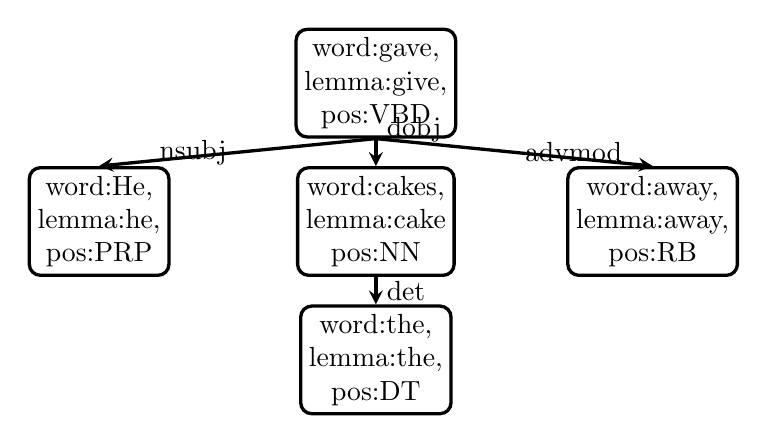
\begin{tikzpicture}[tree-style,level distance=5em,]
\node[pattern-node] {word:gave,\\lemma:give,\\pos:VBD}
 child {node[pattern-node] {word:He,\\lemma:he,\\pos:PRP} edge from parent node[left] {nsubj} }
 child {node[pattern-node]{word:cakes,\\lemma:cake\\pos:NN} 
 	child { node[pattern-node]{word:the,\\lemma:the,\\pos:DT} edge from parent node[right] {det}} 
 	edge from parent node[above right] {dobj} }
 child {node[pattern-node] {word:away,\\lemma:away,\\pos:RB} edge from parent node[right] {advmod}};
\end{tikzpicture}
\caption{Dependency graph example with FS nodes and edges}
\label{fig:dep-graph}
\end{figure}


\begin{definition}[Constituency Graph]\label{def:constituency-graph}
	A \textit{constituency graph} is a feature rich digraph whose nodes $V$ correspond to SFL \textit{units} and carry the \textit{unit class} and the element function within the parent unit (except for the root node); while the edges $E$ represent constituency relations between constituents. 
    %carry mainly the constituency relation between parent and daughter nodes but also potentially other relation types. 
\end{definition}

The basic features of a constituent node are the \textit{unit class} and the function(s) it takes, which is to say the \textit{element(s)} it fills in the parent unit (as described in the discussion of theoretical aspects of SFL in Chapter \ref{ch:sfg}). The root node (usually a clause) is an exception and it does not act as a functional element because it does not have a parent unit. The leaf nodes carry the same features as the DG nodes plus the word class feature which correspond to the traditional part of speech tags. 


\begin{figure}[!ht]
\centering
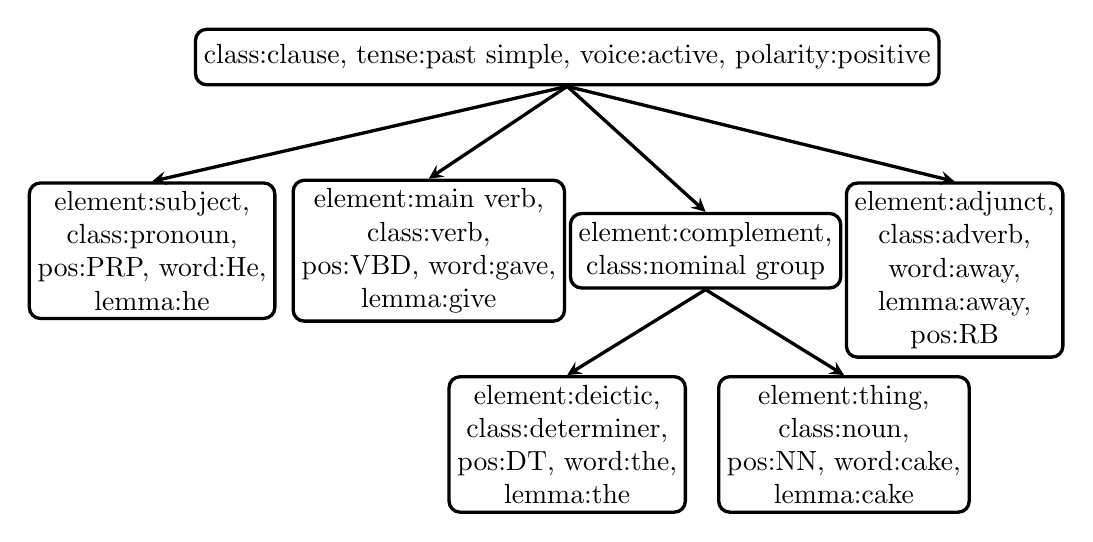
\begin{tikzpicture}[tree-style,]
\node (cla) [pattern-node] {class:clause, tense:past simple, voice:active, polarity:positive}
	child { node (sub)[pattern-node] {element:subject,\\class:pronoun,\\pos:PRP, word:He,\\lemma:he}}		
	child { node (mv)[pattern-node] {element:main verb,\\class:verb,\\pos:VBD, word:gave,\\lemma:give}}
	child { node (com)[pattern-node] {element:complement,\\class:nominal group}
	      child { node (det)[pattern-node]{element:deictic,\\class:determiner,\\pos:DT, word:the,\\lemma:the}}
	      child { node (nou)[pattern-node]{element:thing,\\class:noun,\\pos:NN, word:cake,\\lemma:cake}}}
	child {node[pattern-node,xshift=-1em,yshift=-0.7em](adjunct)
			{element:adjunct,\\class:adverb,\\word:away,\\lemma:away,\\pos:RB}
};
\end{tikzpicture}
\caption{Constituency graph example}
\label{fig:cg-graph}
\end{figure}

Apart from the essential features of class and function, the CG nodes carry additional class specific features selected from the relevant system network. The features considered in this thesis are described in Chapter \ref{ch:the-grammar}. In addition, the leaf CG nodes contain the features of dependency graph nodes enumerated in Definition \ref{def:dep-graph}. The way CG is enriched with features is described in the next chapter. Below in Figure \ref{fig:cg-graph}, is an example CG that carries tense, modality and polarity features on the clause node in addition to class and element function.
%Next section describes simple graph queries and two types of special graph traversal: the conditional and the generative ones. 

\section{Graph traversal}
From the general set of operations on graphs defined in graph theory \citep{bondy1976graph, west2001graph} graph traversal in particular is of importance for the current work. It is used for the constituency graph creation step presented in the parsing pipeline from Figure \ref{fig:pipeline-overview} (in Section \ref{sec:architecture}). The constituency graph is created throughout the traversal of a dependency graph. Traversal is used in this thesis for dependency graphs only.  Next I address this operations in detail.

\tikzset{
    cir1/.style={
        circle,
        draw=black, very thick,
        minimum height=2em,
        inner sep=0.3em,
        text centered,
        align=center,
        anchor=center
    },
    cir2/.style={
        circle,
        draw=black, very thick, dashed,
        minimum height=2em,
        inner sep=0.3em,
        text centered,
        align=center,
        anchor=center
    }
}

\begin{figure}[!ht]
    \centering
    \begin{tikzpicture}[level distance=4em,sibling distance=4em,]
    
    \node (a1) [cir1] {1}
    child { node (a2)[cir1] {2}
        child { node (a5)[cir2] {5} } 
        child { node (a6)[cir1] {6} }
    }
    child { node (a3)[cir2] {3}}		
    child { node (a4)[cir1] {4}
        child { node [cir2] {7} } 
        child { node [cir2] {8} }
    };
    \end{tikzpicture}
    \caption{Sample graph with numbered node of two types}
    \label{fig:example-traversal1}
\end{figure}


%Another important notion that needs to be addressed is the comparison of graph nodes to each other and deciding whether two of them are the ``same'' in some sense or \textit{congruent}. 
%Latter in this chapter we will see that the important operations such as pattern matching depend on comparing nodes to derive whether they are ``the same''. 

%%%%
%% todo remove congruence; good congruence; good
%%%%
%Lets start with node comparison. The simplest form of equivalence, in the labelled graphs such as the one in Figure \ref{fig:example-traversal1}, is the equality of label values. In this example there are no two nodes that are the same because each of them have a unique label. But if we extend the notion of ``sameness'' from the equality of value to some other condition (or rule) then the mathematical term that captures this concept best is that of \textit{congruence} defined in Definition \ref{def:congreunce}. Lets take for example a simple arithmetic rule such as division by 2 which distinguishes odd and even nodes. Under this rule, two nodes are congruent if both are either even or both are odd. In Figure \ref{fig:example-traversal1} the nodes \{2, 4, 6, 8\} are congruent to each other because they are even and conversely the nodes \{1, 3, 5, 7\} are congruent as well. Another example of congruence rule is the node type distinction into continuous line circles and dashed line circles. Under this rule, in Figure \ref{fig:example-traversal1}, the nodes \{3, 5, 7, 8\} are congruent because they are dashed and the rest are congruent because they are in continuous line circles. 
%
%\begin{definition}[Congruence]\label{def:congreunce}
%    A \textit{congruence relation} (or congruence), denoted $\equiv$, is an equivalence relation on a structure that is compatible with the structure. Every congruence relation has a corresponding \textit{quotient} rule (or condition) forming an \textit{equivalence class} (or congruence class) for the relation \citep[26-27]{hungerford1980algebra}.
%\end{definition}
%
%In the case of sets or feature structures the congruence quotient rule needs to be defined corresponding to the structure. An example rule for set congruency can be the threshold of 2 elements on size of the set. Given three sets A=\{0, 1, 2\}, B=\{1, 2\}, C=\{5\}, D=\{6\}, under the above quotient rule, $A \equiv B$ and $C \equiv D$ forming the equivalence classes \{A, B\} and \{C, D\}. In Section \ref{sec:graph-matching} I will return to congruence relation between feature structures and will provide specific (quotient) rules that define equivalence between sets and feature structures. 

%%%%
%% end of congruence; good congruence; good
%%%%

%Lets turn now to queries over the graph nodes and edges. The notion of a query, defied in Definition \ref{def:query}, is tightly linked to the notion of congruence. The query is an operation that selects all the nodes or entities corresponding to a congruence class given by a quotient rule (or constraint) on a graph structure. For example in Figure \ref{fig:example-traversal1} a potential query is to return the equivalence class of the dashed nodes \{3, 5, 7, 8\}. The query operation can be extended to the the graph edges. 
%%In a given dependency graph, similar operation can be used to select all the determiner nodes. In that case we query the nodes with the condition that the part of speech has DT value i.e. \textit{pos=DT}. The same can be achieved by selecting all the edges connecting a noun to its determiner, then the query is formulated for all edges whose relation type is \textit{rel=det}.
%
%\begin{definition}[Graph query]\label{def:query}
%    %Given a graph $G=(V,E)$ to query nodes or edges is to select a set of nodes or a set of edges that satisfy the query constraint condition on feature structure.
%    Given a graph $G(V,E)$ and a query structure $F$, querying $q_{V}(F,G)$ or $q_{E}(F,G)$ over the nodes $V$ or edges $E$ of a graph $G$ is an operation that returns a set of nodes or edges equivalent to the query structure, $ \forall v \in V,  v \equiv F$. 
%\end{definition}

The \textit{graph traversal} defined in \ref{def:traversal} and especially its conditional and generative extensions defined in Definition \ref{def:conditional-traversal} and \ref{def:generative-traversal} are  important operations in this work. They are employed in the first phase of the algorithm, for copying the dependency graph as constituency graph described in Chapter \ref{ch:parsing-algorithm}. 

\begin{definition}[Traversal]\label{def:traversal}
    Traversal $t(V_S,G)$ of a graph $G$ starting from node $V_S$ is a recursive operation that returns a set of sequentially visited nodes neighbouring each other in either \textit{breadth first} ($t_{BF}$) or \textit{width first} ($t_{WF}$) orders.
\end{definition}

The graph traversal is employed either for searching for a node or an edge or finding a sub-graph that fulfils certain conditions on its nodes and edges if it is a conditional traversal. For example in the semantic enrichment phase (that will be described in Section \ref{sec:enrichment-stage}), to ensure that the semantic patterns are applied iteratively to each clause, from a multi-clause CG graphs are selected all clause sub-graphs without including the embedded (dependent) clauses. 

%Using sub-graphs for performing the pattern matching, like in the case of semantic enrichment, decreases drastically the complexity of the graph isomorphism problem (described in Section \ref{sec:graph-matching}) thus increasing the overall performance. 

\begin{definition}[Conditional Traversal]\label{def:conditional-traversal}
    Conditional traversal $t(F_V,F_E,V_S,G)$ of the graph $G$ starting from node $V_S$ under node conditions $F_V$ and edge conditions $F_E$ is a traversal operation where a node is visited if and only if its feature structure conditionally fulfils the $F_V$ and the edge that leads to this node conditionally fulfils the $F_E$.
\end{definition}

One of the potential complete traversals for the graph from Figure \ref{fig:example-traversal1} starting from the node 1 is \{1, 2, 3, 4, 5, 6, 7, 8\} using breadth first strategy or \{1, 2, 5, 6, 3, 4, 7, 8\} for depth first strategy. On the other hand, a conditional traversal of non-dashed nodes staring from the node 1 results in \{1, 2, 4, 6\}, \{1, 4, 2, 6\} or \{1, 2, 6, 4\}. The first two traversals corresponding to the width first strategy and the third one to the depth first strategy. 

I also use the graph traversal to execute generative operations on a parallel graph, which is a special case of \textit{graph rewriting}. For example DG traversal is employed for bootstrapping (i.e. creating in parallel) the CG as it was previously motivated in Section \ref{sec:architecture}.

\begin{definition}[Generative Traversal]\label{def:generative-traversal}
    Generative traversal $g(M,G)$ of a source graph $G$ via a operation matrix $M$ is an operation resulting in the creation of the target graph $H$ by contextually applying generative operations to bring the latter into existence. The operation matrix $M$ is a set of tuples $(ctx,o,p)$ that link the visited source node context $ctx$ (as features of the node, the edge and previously visited neighbour) to a certain operation $o$ that shall is executed on the target graph $H$ with parameters $p$.
\end{definition}

\tikzset{
    sqr1/.style={
        rectangle,
        draw=black, very thick,
        minimum height=0.5em,
        inner sep=0.5em,
        text centered,
        align=center,
        anchor=center
    }
}

\begin{figure}[!ht]
    \centering
    \begin{subfigure}[t]{0.28\textwidth}
        \centering
        \begin{tikzpicture}[scale=1]
        \node (a1) [cir1] { };
        \node (a11) [right =0.1em of a1] {= create};
        \node (a2) [cir2, below =2em of a1] { };
        \node (a21) [right =0.1em of a2] {= extend};
        \end{tikzpicture}
        \caption{The rule set}
        \label{fig:example-traversal00}
    \end{subfigure}
    \begin{subfigure}[t]{0.3\textwidth}
        \centering
        \begin{tikzpicture}[scale=1][level distance=4em,sibling distance=4em,]
        \node (a1) [sqr1] {a}
        child { node (a2)[sqr1] {b}
            child { node (a5)[sqr1] {d} } 
        }
        child { node (a3)[sqr1] {c}};
        \end{tikzpicture}
        \caption{The target}
        \label{fig:example-traversal21}
    \end{subfigure}
    \begin{subfigure}[t]{0.4\textwidth}
        \centering
        \begin{tikzpicture}[scale=1][level distance=4em,sibling distance=8em,]
        \node (a1) [sqr1] {a: \{1, 3\}}
        child { node (a2)[sqr1] {b: \{2, 5\}}
            child { node (a5)[sqr1] {d: \{6\}} } 
        }
        child { node (a3)[sqr1, right=1em of a2] {c: \{4, 7, 8\}}};
        \end{tikzpicture}
        \caption{The explained target}
        \label{fig:example-traversal22}
    \end{subfigure} 
    \caption{The generative traversal result for Figure \ref{fig:example-traversal1} using create and extend operations}
    \label{fig:example-traversal2}
\end{figure}

Next I provide an rough description of what happens when a generative traversal is executed and the exact algorithm will be described in detail in Section \ref{sec:creation-constituency-graph}. For example lets assume that only two types of operation are needed for our task at hand. First is to create a new node on the target graph once a non-dashed node is visited on the source graph. And, second, is to pass without doing anything the dashed nodes. This is schematically represented in Figure \ref{fig:example-traversal00}. Lets now apply these operations on traversing the example graph using breadth first strategy following the order provided above \{1, 2, 3, 4, 5, 6, 7, 8\}. The traversal graph is considered source graph and the target graph is empty at the beginning of the process. Upon visiting the node 1 a first node is created on the target graph which is labelled \textit{a}. When traversing nodes 2 and 4 then each of them signal creation of the nodes \textit{b} and \textit{c} as children of \textit{a} in the target graph and correspondingly node 6 signals creation of node \textit{d}. The final target graph is depicted in Figure \ref{fig:example-traversal21} and in Figure \ref{fig:example-traversal22} the source nodes are embedded into the target node to make explicit that the non-dashed nodes (i.e. 3, 5, 7, 8) are simply passed over without any generative operation. 

Now that generative traversal is defined, by analogy, \textit{update}, \textit{insert} and \textit{delete} traversals can be defined on the source or target graph by using the same mechanism of \textit{operation matrices} mapping contexts of visited nodes and edges to update, insert and delete operations. In this work, however, these operations are not used and therefore omitted here.

In Section \ref{sec:graphs} the last two definitions were for the constituency and dependency graphs. They are used in this thesis to represent grammatical analysis of of a sentence. Next we will look at a special type of graph which represents fragments of structure repeatable across multiple analysis. They represent generalisations or patterns that usually are associated with grammatical features or a set of features which I explain in Chapter \ref{ch:parsing-algorithm}. These graphs are called \textit{pattern graphs} and the next section is dedicated to them.  

\section{Pattern graphs}
\label{sec:pattern-graphs}
Regardless of the type, constituency or dependency, the parsing process (which will be described in Chapter \ref{ch:parsing-algorithm}) relies on identifying patterns in graphs. The patterning is described as both graph structure and feature presence (or absence) in the nodes or edges. The \textit{pattern graphs} (defined in \ref{def:graph-pattern}) are special kinds of graphs meant to represent small (repeatable) parts of parse graphs that, in the context of the current work, are used to identify grammatical features. 

The pattern graphs contrast with the \textit{parse} (or \textit{instance}) graphs which are either constituency or dependency graphs. The parse graphs express what is an actual analysis of a text, i.e. representing what is the case, whereas the pattern graph expresses a potential that could be the case in the instance graph. This way the pattern graphs have a prescriptive interpretation whereas the instance ones taken a factual interpretation. 

%Pattern graphs can also specify operations that shall be executed when the pattern is successfully matched (for example add a new feature on a given node). This kinds of graphs need last four requirements listed in the beginning of this section.

\begin{definition}[Pattern Graph]\label{def:graph-pattern}
    A \textit{pattern graph} (PG) is a feature rich graph for expressing regularities in the node and edge structure.
\end{definition}

%part of the definition: or edge configuration and feature structure including descriptions of \textit{negated nodes or edges} (i.e. absence of), logical operators over feature sets (AND, OR, XOR and NAND) and operations once the pattern is identified in a target graph (select, insert, delete and update).

%The feature structure of a PG are always \textit{underspecified} as compared to the dependency or constituency graph in the sense that irrelevant attribute-value pairs are omitted sometimes down to an empty FS. However often it is useful to specify more than one value for the same feature as a list of disjunctive values allowing the pattern to cover larger set of possible cases. I will call these FS as being \textit{over-specified}. 

%An example of PG is depicted in figure \ref{fig:gp1} in the Section \ref{sec:pattern-graph-matching}. It deals with pattern graph matching and other operations with in detail. But before that I will first briefly cover generic operations on graphs and the problem of graph matching also known in computer science as the \textit{graph isomorphism} problem.

%Before I dive into characterising pattern graph matching and operations with pattern graphs, I 
Next I discuss two example of pattern graphs. One example shows a pattern graph encoding the present perfect continuous tense, which traditional grammar defines as in Table \ref{tab:ppc-pattern}. Afterwards, the second example will show how the notion of linear succession among nodes is accounted for in the pattern graphs for declarative and interrogative mood.

\begin{table}[!ht]
	\centering
	\begin{tabular}{|clclc|}
		\hline
		\textit{has/have}       & + & \textit{been}          & + & \textit{Vb-ing}          \\
		to have, present simple &   & to be, past participle &   & verb, present participle \\ \hline
	\end{tabular}
	\caption{Present perfect continuous tense}
	\label{tab:ppc-pattern}
\end{table}

Examples \ref{ex:ppc1}--\ref{ex:ppc3} show variations of present perfect continuous tense in a simple clause according to declarative and interrogative mood and the ``has'' contraction. Of course there are more variations possible for example according to voice (active and passive) but they are omitted here because they adds combinatorially to the number of examples and the ones provided already serve their purpose here. The Figures \ref{fig:ppc1}-\ref{fig:ppc3} represent corresponding dependency parses for these examples (generated with Stanford dependency parser).

\begin{exe}
	\ex\label{ex:ppc1} He has been reading a text.
	\ex\label{ex:ppc2} He's been reading a text.
	\ex\label{ex:ppc3} Has he been reading a text?
\end{exe}

%\begin{figure}[!ht]
%	\centering
	\begin{figure}[!ht]
		\centering
		\begin{dependency}[dep-style-narrow]
			\begin{deptext}[]
				PRP \& VBZ \& VBN \& VBG \& DT \& NN \\
				He \& has \& been \& reading \& a \& text \\
			\end{deptext}
			\deproot{4}{root}
			\depedge{4}{1}{nsubj}
			\depedge{4}{2}{aux}
			\depedge{4}{3}{aux}
			\depedge{4}{6}{dobj}
			\depedge{6}{5}{det}
		\end{dependency}
		\caption{Present perfect continuous: indicative mood, un-contracted ``has''}
		\label{fig:ppc1}
	\end{figure}

	\begin{figure}[!ht]
        \centering
		\begin{dependency}[dep-style-narrow]
			\begin{deptext}[]
				PRP \& VBZ \& VBN \& VBG \& DT \& NN \\
				He \& 's \& been \& reading \& a \& text \\
			\end{deptext}
			\deproot{4}{root}
			\depedge{4}{1}{nsubj}
			\depedge{4}{2}{aux}
			\depedge{4}{3}{aux}
			\depedge{4}{6}{dobj}
			\depedge{6}{5}{det}
		\end{dependency}
		\caption{Present perfect continuous: indicative mood, contracted ``has'' }
		\label{fig:ppc2}
	\end{figure}
%\end{figure}
%
\begin{figure}[!ht]
	\centering
	\begin{dependency}[dep-style]
		\begin{deptext}[]
			VBZ \& PRP \& VBN \& VBG \& DT \& NN \\
			Has \& he \& been \& reading \& a \& text \\
		\end{deptext}
		\deproot{4}{root}
		\depedge{4}{2}{nsubj}
		\depedge{4}{1}{aux}
		\depedge{4}{3}{aux}
		\depedge{4}{6}{dobj}
		\depedge{6}{5}{det}
		%\depedge[collage]{5}{6}{dobj}
	\end{dependency}
	\caption{Present perfect continuous: interrogative mood, un-contracted ``has''}
	\label{fig:ppc3}
\end{figure}


The present perfect continuous tense can be formulated as a pattern graph (including voice) over the dependency structure as illustrated in Figure \ref{fig:gp1}.
In this pattern the main lexical verb is \textit{present participle} indicated via the \textit{VBG} part of speech. It is accompanied by two auxiliary verbs: \textit{to be} in \textit{past participle} (\textit{VBN}) form and \textit{to have} in \textit{present simple} form specified by either \textit{VBZ} for 3rd person or \textit{VBP} for non-3rd person. Also the \textit{to be} can be either connected by the \textit{aux} relation or in case of passive form by the \textit{auxpass} relation. Note that the pattern in Figure \ref{fig:gp1} constraints the edge type (using an OR-set) to the verb \textit{to be} which can be either \textit{aux} or \textit{auxpass} and the part of speech of the verb \textit{to have} which can be \textit{VBZ} or \textit{VBP}.

\begin{figure}[!ht]
    \centering
    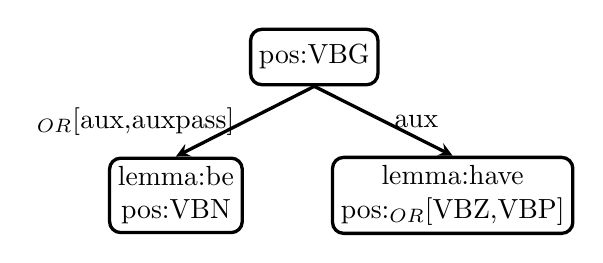
\begin{tikzpicture}[tree-style,level distance=5em,]
    \node[pattern-node, anchor=center] (vb1){pos:VBG}
    child {node[pattern-node] {lemma:be\\pos:VBN} edge from parent node[left] {$_{OR}$[aux,auxpass]} }
    child {node[pattern-node] {lemma:have\\pos:$_{OR}$[VBZ,VBP]} edge from parent node[right] {aux}};
    \end{tikzpicture}
    \caption{The graph pattern capturing features of the present perfect continuous tense}
    \label{fig:gp1}
\end{figure}

One of the fundamental features of language is its sequentiality and directionality. This aspect is not inherent in graphs. In the simplest form, they just describe connections between nodes and are agnostic to any meaning or interpretation. Next, I introduce the way I deal with linear order in the pattern graphs. 

%To demonstrate how the order will specified in the graph patterns, 
Lets consider the clause mood and encode the distinction between \textit{declarative} and \textit{Yes/No interrogative} moods. In SFG this features is described in terms of the relative order of clause elements. If the finite is before the subject then the mood is Yes/No-interrogative, whereas when the finite succeeds subject then the mood is declarative. Example \ref{ex:ppc3} contrasts in mood with \ref{ex:ppc1} and \ref{ex:ppc2}. 

Order can be specified in absolute or relative terms and partially or exhaustively. In order to cover these three kinds of constraints, I introduce three special features: the node \textit{id}, \textit{precede} and \textit{position}. Node id takes a token to uniquely identify a node in the graph, the precede feature takes an ordered set to indicate the (partial) linear precedence to other node ids, and the position feature indicates the absolute position of a node.

One way to introduce order among nodes is then by marking them with an absolute position. This is a good method applicable to parse graphs. The DGs and CGs, are automatically assigned at creation time the absolute position of the node in the sentence text via the feature \textit{position}. This feature is present in the leaf nodes only and corresponds to the order number in which they occur in the sentence text while the non-leaf node's position is considered to be the lowest position of its constituent nodes. The absolute position description is rarely used in the PGs. The only cases are to state that the constituent is first or last position in a sentence.  %In the 

Another way to specify node order is through relative precedence, for which the node id and the precedence features are introduced above. This is the preferred method to provide linear precedence dimension in pattern graphs. It is also relative so the specification can be partial. With this method a node specifies that it precedes a set of other nodes. 

	\begin{figure}[!ht]%{0.4\textwidth}
		\centering
		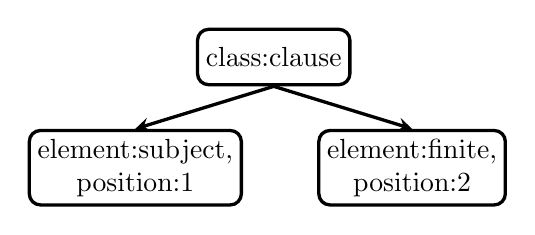
\begin{tikzpicture}[tree-style,,level distance=4em,]
		\node (cla) [pattern-node] {class:clause}
		child { node (sub)[pattern-node] {element:subject,\\position:1}}		
		child { node (f)[pattern-node] {element:finite,\\position:2}};
		\end{tikzpicture}
		\caption{Declarative mood pattern graph with absolute element order}
		\label{fig:pg-declarative}
	\end{figure}
	\begin{figure}[!ht]%{0.4\textwidth}
		\centering
		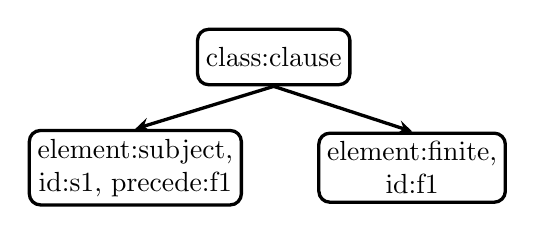
\begin{tikzpicture}[tree-style,,level distance=4em,]
		\node (cla) [pattern-node] {class:clause}
		child { node (sub)[pattern-node] {element:subject,\\id:s1, precede:f1}}		
		child { node (f)[pattern-node] {element:finite,\\id:f1}};
		\end{tikzpicture}
		\caption{Declarative mood pattern graph with relative element order}
		\label{fig:pg-declarative2}
	\end{figure}
    \begin{figure}[!ht]
    	\centering
    	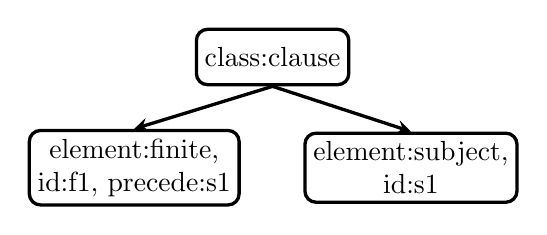
\begin{tikzpicture}[tree-style,,level distance=4em,]
    	\node (cla) [pattern-node] {class:clause}
    	child { node (f)[pattern-node] {element:finite,\\id:f1, precede:s1}}
    	child { node (sub)[pattern-node] {element:subject,\\id:s1}}	;	
    %	child { node (mv)[pattern-node] {element:main verb,\\id:mv1}};
    	\end{tikzpicture}
    	\caption{Pattern graph for Yes/No interrogative mood}
    	\label{fig:pg-interrogative}
    \end{figure}

To continue the example of mood features, I illustrate in Figures \ref{fig:pg-declarative} and \ref{fig:pg-declarative2} the use of relative and absolute node ordering constraints for declarative mood; and in 
Figure \ref{fig:pg-interrogative}, I depict the PG for the Yes/No interrogative mood. In both cases I use the relative node ordering.

%todo: explain what negative nodes are

%From the usability point of view there are few technicalities I shall emphasize. First, the precedence feature can be used on any node. When matched, the precedence declarations are collected from all nodes into a single set before being checked. However I recommend as a good practice to specify the order of nodes on the parent constituent. 
%
%Second, the notation in Figure \ref{fig:pg-interrogative} follows the Python bracketing meaning i.e. the round brakes signify tuples while the square ones lists (ordered sets). So the main verb element is redundant and is introduced to demonstrate multiple order specifications. However the order can be either specified as a set of binary tuples or as an ordered set (i.e. a Python list). So precedence:[(f1,s1),(s1,mv1)] is equivalent to precedence:[f1,s1,mv1]. 
%
%Thirdly the ordering can be defined in absolute terms via position or in relative terms. Note that in the case of PGs the absolute ordering of nodes is interpreted relatively so PG in figure \ref{fig:pg-declarative} is identical to \ref{fig:pg-declarative2}.


Patterns like the ones explained above can be created for a wide range of grammatical features. Once the grammatical feature is encoded as a pattern graph it can be identified in parse graphs (DG or CG) via \textit{graph pattern matching} operation described in Section \ref{sec:graph-matching}. Moreover, once the pattern is identified it can act as a triggering condition for the node update operation. When the pattern is matched then additional features can be added to the nodes of the parse graph thus the mechanism of enriching the parse graph. Coming back to out tense example above, once the pattern \ref{fig:gp1} is identified then the clause can be marked with the tense feature. In the next section I address the graph matching operation and then show how it works using pattern graphs. 

% skip:complicated, unclear, compressed
%But such traversal operations cannot be easily defined. While traversal context may be sufficient for generative operations on a new structure, it is insufficient for executing affecting operations on the traversed graph. To overcome this limitation, instead of using traversal context I take a different approach: the \textit{pattern graphs}, defined in previous section combined with generic graph matching algorithm. This mechanism offers a similar algorithmic independence of mapping structural context to operation(s) triggered by it. 

\section{Graph matching}
\label{sec:graph-matching}

So far we have discussed about constituency and dependency graphs and, in the last section, I introduced pattern graphs. The intuition behind pattern graphs is that they are meant to be matched against or found in other graphs. The patterns graphs can be viewed as small reusable modules and as generalizations consisting of structural patterns. I will address next what does it mean for two graphs to be the same, i.e. \textit{isomorphic} and how this sameness checking is used in the current work. 

In \textit{mathematics} the structure-preserving mappings $f:X \rightarrow Y$ (from one object $X$ to the other $Y$) of the same type is called \textit{morphism}. The morphism $f:X \rightarrow Y$ is called \textit{isomorphism} if there exists an inverse morphism $g:Y \rightarrow X$ such that $f \circ g = id_{X}$ and $ g \circ f = id_{X}$.

%\begin{definition}[Morphism]\label{def:morphism}
%    A morphism $f:X \rightarrow Y$ is a structure preserving map from one object $X$ to the other $Y$ where the objects are complex structures such as sets, feature structures or graphs.
%\end{definition}
%
%
%\begin{definition}[Isomorphism]\label{def:isomorphism}
%    The morphism $f:X \rightarrow Y$ is called \textit{isomorphism} if there exists an inverse morphism $g:Y \rightarrow X$ such that $f \circ g = id_{X}$ and $ g \circ f = id_{X}$.
%\end{definition}

In computer science, the \textit{graph matching} operation is known (sub-)graph isomorphism. Two graphs $G=(V_G,E_G)$ and $H=(V_H,E_H)$ are isomorphic if there exists a mapping from the nodes of graph $G$ to the nodes of graph $H$, such that the edge neighbourhood is preserved. In such context the nodes are unique atomic symbols functioning as node identifiers. 
 

\begin{definition}[Graph matching]\label{def:gmatching}
    For two graphs $G$ and $H$, where $G \leq H$, \textit{graph matching} is the operation of finding an isomorphism between $G$ and $H$.
\end{definition}

\begin{definition}[Graph isomorphism]\label{def:gisomorphism}
    An isomorphism of graph $G=(V_G,E_G)$ and $H=(V_H,E_H)$ is a bijective function $f:V_G \rightarrow V_H$ such that if any two nodes  $u,v \in V_G$ from $G$ are adjacent $(u,v) \in E_G$ then $f(u), f(v)$ are adjacent in $H$ as well $(f(u), f(v)) \in E_H $.
\end{definition}

%\begin{definition}[Graph matching]\label{def:gmatching0}
%    For two given graphs $G$ and $H$ \textit{graph matching} is the operation of testing whether $G$ is structurally isomorphic to $H$.
%\end{definition}

Graphs do not always have the same number of nodes (or edges). We say that a graph is smaller than another one, denoted $G \leq H$, when its number of nodes is less than that of the other graph. In such cases, for two graphs $G$ and $H$ where $G<H$, the (sub-)graph matching task is redefined to establishing isomorphism(s) from $G$ to a sub-graph of $H$. 
%In this case, the mapping function is relaxed from bijective (perfect mapping from first to second graph) to an injective one (each node from first has a correspondent in the second one).

\begin{definition}[Sub-graph isomorphism]\label{def:sgisomorphism}
       Given two feature rich graphs $G=(V_G,E_G)$ and $H=(V_H,E_H)$, $G$ is sub-graph isomorphic to $G$ (denoted $G \subseteq H$) if there is an injective function $f:V_G \rightarrow V_H$ such that
   \begin{itemize}
       \item $\forall v \in V_G, f(v) \in V_H$ and
       \item any two nodes adjacent in $G$, $(u,v) \in E_G$, are also adjacent in $H$, $(f(u), f(v)) \in E_H $
   \end{itemize}
\end{definition}


\begin{figure}[!ht]
    \centering
    \begin{subfigure}[t]{0.48\textwidth}
        \centering
        \begin{tikzpicture}[scale=1]
        \node (a1) [cir1] {1};
        \node (a2) [cir1, right =3em of a1] {2};
        \node (a3) [cir1, below =3em of a1] {3};
        
         \draw[sequence,->] (a1) -- (a2);
         \draw[sequence,->] (a2) -- (a3);
         \draw[sequence,->] (a3) -- (a1);
        
        \end{tikzpicture}
        \caption{The pattern graph}
        \label{fig:example-matching1}
    \end{subfigure}
    \begin{subfigure}[t]{0.48\textwidth}
        \centering
        \begin{tikzpicture}[scale=1][level distance=4em, sibling distance=4em,]
        \node (a1) [cir1] {a};
        \node (a2) [cir1, right =3em of a1] {b};
        \node (a3) [cir1, below =3em of a1] {c};
        \node (a4) [cir1, below =3em of a2] {d};
        
        \draw[sequence,->] (a1) -- (a2);
        \draw[sequence,->] (a2) -- (a3);
        \draw[sequence,->] (a3) -- (a1);
        \draw[sequence,->] (a2) -- (a4);
        
        \end{tikzpicture}
        \caption{The target graph}
        \label{fig:example-matching2}
    \end{subfigure}
    \caption{Sub-graph isomorphism \{1=a, 2=b, 3=c\}}
    \label{fig:example-matching}
\end{figure}

In Figure \ref{fig:example-matching1} is depicted a labelled graph that is isomorphic to a sub-graph in Figure \ref{fig:example-matching2}. The example graphs presented in Figure \ref{fig:example-matching} have atomic labels as nodes and the isomorphism is established as a mapping between labels. Section \ref{sec:graphs} above mentions that the graph considered in this thesis have feature structures as their nodes and not atomic nodes. But in case of feature rich graphs additional rules how to establish the isomorphism need to be provided because there are multiple ways to approaching it. 

\begin{figure}[!ht]
    \centering
    \begin{subfigure}[t]{0.38\textwidth}
        \centering
        \begin{tikzpicture}[scale=1]
        \node (a1) [pattern-node] {f_1: 1 \\ f_2: scissors};
        \node (a2) [pattern-node, right =3em of a1] {f_1: 2 \\ f_2: paper};
        \node (a3) [pattern-node, below =3em of a1] {f_1: 3 \\ f_2: rock};
        
        \draw[sequence,->] (a1) -- (a2);
        \draw[sequence,->] (a2) -- (a3);
        \draw[sequence,->] (a3) -- (a1);
        
        \end{tikzpicture}
        \caption{The pattern graph}
        \label{fig:example-r-matching1}
    \end{subfigure}
    \begin{subfigure}[t]{0.58\textwidth}
        \centering
        \begin{tikzpicture}[scale=1][level distance=4em, sibling distance=4em,]
        \node (a1) [pattern-node] {f_1: a \\ f_2: scissors};
        \node (a2) [pattern-node, right =3em of a1] {f_1: b \\ f_2: paper};
        \node (a3) [pattern-node, below =3em of a1] {f_1: c \\ f_2: rock};
        \node (a4) [pattern-node, below =3em of a2] {f_1: d \\ f_2: scissors};
        \node (a5) [pattern-node, right =3em of a4] {f_1: e \\ f_2: rock};
        
        \draw[sequence,->] (a1) -- (a2);
        \draw[sequence,->] (a2) -- (a3);
        \draw[sequence,->] (a3) -- (a1);

        \draw[sequence,->] (a2) -- (a4);
        \draw[sequence,->] (a4) -- (a5);
        \draw[sequence,->] (a5) -- (a2);
        
        \end{tikzpicture}
        \caption{The target graph}
        \label{fig:example-r-matching2}
    \end{subfigure}
    \caption{An example of rich sub-graph isomorphism}
    \label{fig:example-r-matching}
\end{figure}

Lets look at Figure \ref{fig:example-r-matching} where the graph nodes are feature structures using features: f_1 and f_2. One way to approach isomorphism in this scenario is by the value of one feature, for example f_1. Then we can identify two sub-graph isomorphisms: \{1=a, 2=b, 3=c\} and \{1=b, 2=d, 3=e\}. This approach, besides additional specification what values to compare, i.e. f_1s, is the same as providing a sub-graph isomorphism on the labelled graphs from Figure \ref{fig:example-matching}. 

In addition to the rule above, lets add a constraint that the isomorphism is not only a mapping between the feature values (numbers to letters) but also that the mapped values are identical (strict value equality). 
If we consider the strict equality rule applied on f_1 feature, there is no isomorphism between the two graphs because first one uses numbers  \{1, 2, 3\} and the second uses letters\{a, b, c, d\}. Now if we turn to the values of f_2 and apply the same rule then there is one isomorphism possible \{paper=paper, rock=rock, scissors=scissors\}. The second one, even if it is a cycle, \{paper=paper, rock=scissors, scissors=rock\} is no longer acceptable because the ``scissors'' and ``rock'' switched places in the target graph and it would have been acceptable as a mapping, but not as strict value equality. Formally, the additional equality constraint can be expressed on the graph isomorphism $f$ as $u=f(u)$.

This brings us to the idea that, in the feature rich (sub-)graph isomorphism, we need to introduce a \textit{matching} operator (denoted $\match$) for nodes. This means that we no longer can use atomic symbol mapping but have to employ the matching operator. The node matching operation is defined on feature structures. We say that a feature structure may match once, several times or not at all another feature structure, $FS_1 \match FS_2$. This intuition is expressed in Definition \ref{def:fs-match}. The sub-graph isomorphism over the feature rich graphs is captured in Definition \ref{def:rsgisomorphism} below.

%For graph matching definition this implies that the node label equality operation is replaced with matching criteria is the method to impose an additional set of constraints on the graph isomorphism and allow comparison of complex nodes such as those in feature rich graphs. 
 
%The rich graph matching operation can be also seen as a search for rich sub-graph isomorphism. 

\begin{definition}[Rich sub-graph isomorphism]\label{def:rsgisomorphism}
    Given two feature rich graphs $G=(V_G,E_G)$ and $H=(V_H,E_H)$ and a matching relation $\match$, $G$ is sub-graph isomorphic to $H$ if there is an injective mapping $f:V_G \rightarrow V_H$ such that
    \begin{itemize}
        \item each node in $V$ is mapped to exactly one node in $H$, $\forall v \in V_G, f(v) \in V_H$ and
        \item each node in $G$ matches with its correspondent in $H$, $\forall v \in V_G, v \gtrdot f(v)$ and
        \item any two nodes which are adjacent in $G$, are also adjacent in $H$, $\forall (u,v) \in E_G, \exists \big(f(u), f(v)\big) \in E_H $
    \end{itemize}
\end{definition}

%\begin{definition}[Rich Graph Matching]\label{def:rgmatching}
%    For two feature rich graphs $G$ and $H$ where $H \leq G$ and an \textit{identity settling function} $idx_{V}$, the \textit{rich graph matching} is the function that finds a structural isomorphism between $H$ and $G_{1} \subseteq G$ provided that for all nodes $V_{i} \in H$ their \textit{morphism function} $V_{j} \in G_{1}$ 
%    
%    satisfies the identity function $f_{V}(V_{i})=V_{j}$ 
%\end{definition}

%The congruency rules (also referred in the implementation as \textit{identity} or \textit{equivalence functions}) used in this work will be provided in the Section \ref{sec:pattern-graph-matching} below. They are contextualised to the graph matching operation between pattern graphs and dependency and constituency graphs. 
%
%\section{Pattern graph matching}
%\label{sec:pattern-graph-matching}

We already mentioned in the introduction of this section that pattern graphs are considered as generalizations over parse graphs (constituency or dependency). The pattern graphs are smaller and their nodes have fewer features specified. The parse graphs have more nodes and features. We say that a parse graph \textit{instantiates} a pattern graph if there exists a rich sub-graph isomorphism. This operation is called \textit{pattern graph matching} and is defined in Definition \ref{def:fs-match} below. 

\begin{definition}[Pattern graph matching]\label{def:pgmatching}
    Given a pattern graph $G$ and an instance (parse) graph $H$ (either dependency or constituency), \textit{pattern graph matching} is the operation of finding a rich sub-graph isomorphism from $G$ to $H$ such that each pattern node matches its corresponded instance node each $H$, $\forall v \in V_G, v \gtrdot f(v)$.
\end{definition}

%The pattern and parse graphs are feature rich graphs. This means that the nodes are feature structures. In the previous section the rich graph matching require definition of congruence rules and in this case it is between two feature structures. 

As mentioned before, nodes of the parse and the pattern graphs are feature structures. I approach the matching between them in two steps: first, matching the feature names in Definition \ref{def:fs-match}, and second,  matching the feature values in Table \ref{tab:strict}. 
In order to simplify and make explanations clear, I will further refer to the feature structures that constitute nodes in the pattern graphs as \textit{pattern feature structures} and the feature structures that constitute nodes in the instance graphs as \textit{instance feature structure}.

\begin{definition}[Feature structure matching]\label{def:fs-match}
    A pattern feature structure $V$ matches an instance feature structure $U$ if and only if every feature in $V$ has a corresponding feature $U$ and their values match; that is $ \forall f_V \in V, \exists f_U$ such that $name(f_V) = name(f_U)$ and $ val(f_V) \match val(f_U)$.
\end{definition}

%Next is defined matching of the feature values. 
According to the Definition \ref{def:fs}, the values of feature structures can be either atomic (numbers, strings, symbols, etc.), denoted $atomic$, or one of the conjunction sets: $S_{AND}$, $S_{OR}$, $S_{XOR}$ and $S_{NAND}$. For simplicity, the option of nested feature structures is excluded in the current work even though it is perfectly viable configuration. Consequently, the matching relation takes into consideration the \textit{type} of the compared elements in addition to how they relate to each other, including comparisons between set and atomic values. 
Please note that this relation is \textit{not symmetric} i.e. \textit{not commutative} because the subsequent relations used in the definition i.e. set inclusion and set subsumption are not symmetric. This means that $A \match B \neq B \match A $. 
%Finally, these definitions create equivalence sets \textit{relative} to one of the compared elements and not absolute equivalence sets. For example the division by 2, is an absolute condition for two numeric elements to belong to the same equivalence class either of odd or that of even numbers. By contrast, if we consider set inclusion between two sets $A \subseteq B$ as a condition for set element equivalence then it generates two possible equivalence sets. First, all sets $X$ that are subsets of $B$, $\forall X, X \subseteq B$ and second, all sets Y that include $A$,  $ \forall Y, A \subseteq Y $. 

I will remind here that, the function $\tau(S)$, defined in Section \ref{sec:graphs}, returns the \textit{type} of the feature value. I extend its definition here to handle also atomic data types as follows $\tau:x \rightarrow \{atomic, S_{AND}, S_{OR}, S_{XOR}, S_{NAND} \}$. The matching rules have to be defined for each possible pair of types returned by the function $\tau$ yielding 25 possibilities. Table \ref{tab:strict} provides matching relations for each pair of types where the rows represent value types of the pattern features, denoted $\tau(v)$, and the columns represent value types of the instance features, denoted $\tau(u)$. Each table cell contains a comparison expression returning a truth value. Cells with a bottom sign $\bot$ mean that there can be no match between these types no matter the values. 
%I use set theoretic notations such as set inclusion $\subseteq$, intersection $\cup$ and set membership $\in$. 

\begin{table}[!ht]
    \centering
    \begin{tabular}{|c|c|c|c|c|c|}
        \hline
        \textit{$\tau(v)$\textbackslash $\tau(u)$} & \textit{atomic} & \textit{S_{AND}}                 & \textit{S_{OR}}              & \textit{S_{XOR}}             & \textit{S_{NAND}}            \\ \hline
        \textit{atomic}             & $v=u$             & $v \in u$                         & $\bot$                          & $\bot$                          & $v \notin u$                   \\ \hline
        \textit{S_{AND}}              & $\bot$               & $v \subseteq u$                     & $\bot$                          & $\bot$                          & $\bot$ \\ \hline
        \textit{S_{OR}}               & $v \ni u$          & $ v \cap u \neq \varnothing $ &                        $v \supseteq u $              & $v \supseteq u $   & $\bot$ \\ \hline
        \textit{S_{XOR}}              & $v \ni u$          & $\bot$                              & $\bot$                        & $v \supseteq u$             & $\bot$ \\ \hline
        \textit{S_{NAND}}             & $v \not\ni u$      & $v \cap u = \varnothing$     & $v \cap u = \varnothing$ & $v \cap u = \varnothing$ & $ v \subseteq u $                          \\ \hline
    \end{tabular}
    \caption{Strict matching between pattern and instance feature values organised by value type}
    \label{tab:strict}
\end{table}

For example, if both values are of atomic type then in order to match they have to equal. If the $\tau(v)$ is atomic and the $\tau(u)$ is an AND set then $v$ needs to be among the set of values constituting $u$; whereas if the $\tau(u)$ is an OR or XOR set then these values do not match, designated by the bottom sign $\bot$. The same reading applies to the rest of the table for each pair of value types. 

A more permissive matching is defined in Table \ref{tab:permissive}. Here, on the instance feature values, the two types of disjunction (OR and XOR) and the negated conjunction (NAND) are interpreted as possibly matching and provided with the corresponding relation whereas in the previous definition these cases were completely excluded. The permissive match is rarely used in this work but it is nevertheless useful cases of instance graphs where the feature values could not be are assigned with a certainty but as a disjunction of either one or the other. 

\begin{table}[!ht]
    \centering
    \begin{tabular}{|c|c|c|c|c|c|}
        \hline
        \textit{$\tau(v)$\textbackslash $\tau(u)$} & \textit{atomic} & \textit{S_{AND}}                 & \textit{S_{OR}}              & \textit{S_{XOR}}             & \textit{S_{NAND}}            \\ \hline
        \textit{atomic}             & $v=u$             & $v \in u$                         & $v \in u$                          & $v \in u$                          & $v \notin u$                   \\ \hline
        \textit{S_{AND}}              & $\bot$               & $v \subseteq u$                     & $v \subseteq u$                          & $v \subseteq u$                          & $v \cap u = \varnothing$ \\ \hline
        \textit{S_{OR}}               & $v \ni u$          & $ v \cap u \neq \varnothing $ &                        $v \supseteq u $              & $v \supseteq u $   & $v \backslash u \neq \varnothing$ \\ \hline
        \textit{S_{XOR}}              & $v \ni u$          & $\bot$                              & $\bot$                        & $v \supseteq u$             & $ |v \backslash u| = 1$ \\ \hline
        \textit{S_{NAND}}             & $v \not\ni u$      & $v \cap u = \varnothing$     & $v \cap u = \varnothing$ & $v \cap u = \varnothing$ & $ v \subseteq u $                          \\ \hline
    \end{tabular}
    \caption{Permissive matching between pattern and instance feature values organised by value type}
    \label{tab:permissive}
\end{table}


%the old taxt no longer needed
%
%
%When checking the equivalence of two feature values, three cases can be asserted: $x=y$ i.e. $x$ is definitely equal to $y$, $x\neq y$ i.e. $x$ is definitely different from $y$ and $x\sim y$ i.e. $x$ is maybe (or could be) equal to $y$. 
%
%I define below two identity morphisms: (a) \textit{permissive} $I_{permissive}$ (defined by Equation \ref{eq:permissive}) which includes the uncertain cases and (b) \textit{strict} $I_{strict}$ (defined by Equation \ref{eq:strict}) which excludes the uncertain cases. The main difference between the two morphism functions is whether on the right side (the instance graph) any uncertainty is accepted. This is to say any of the disjunctive sets $s_{OR}$ and $S_{XOR}$. 
%
%\begin{definition}[Strict Pattern Graph Matching]\label{def:strict-matching}
%	\textit{Strict pattern graph matching} is a rich graph matching where a morphism for the pattern graph $H$ is found in the target graph $G$ given that $H \leq G$ and that for any node $p \in H$ there is a node $r \in G$ satisfying the strict identity morphism $I_{strict}:p \rightarrow r$
%\end{definition}
%
%
%\begin{equation} \label{eq:strict}
%	I_{strict}:p \rightarrow r \models
%	\begin{cases}
%	p = r, & \text{if}\ T(p) = simple \wedge T(r) = simple \\
%	p \in r, & \text{if}\ T(p) = simple \wedge T(r) = S_{AND} \\
%	p \subseteq r, & \text{if}\ T(p) = S_{AND} \wedge T(r)= S_{AND} \\
%	p \cap r \neq \varnothing, & \text{if}\ T(p) = S_{OR} \wedge T(r) = S_{AND}\\
%	r \in p, & \text{if}\ T(p) = S_{OR} \wedge T(r) = simple \\
%	%p \cap r \neq \varnothing, & \text{if}\ T(p) = S_{XOR} \wedge T(r) \in \{S_{OR}, S_{XOR}\} \\
%	r \in p, & \text{if}\ T(p) = S_{XOR} \wedge T(r) = simple \\
%	p \cap r = \varnothing, & \text{if}\ T(p) = S_{NAND} \wedge T(r) \in \{S_{AND}, S_{OR}, S_{XOR}\} \\
%	r \notin p, & \text{if}\ T(p) = S_{NAND} \wedge T(r) = simple \\
%	\top, & \text{if}\ T(p) = S_{NAND} \wedge T(r) = S_{NAND}
%	\end{cases}
%\end{equation}
%
%\begin{definition}[Permissive Pattern Graph Matching]\label{def:permissive-matching}
%	\textit{Permissive pattern graph matching} is a rich graph matching where a morphism for the pattern graph $H$ is found in the target graph $G$ given that $H \leq G$ and that for any node $p \in H$ there is a node $r \in G$ satisfying the permissive identity morphism $I_{permissive}:p \rightarrow r$
%\end{definition}
%
%\begin{equation} \label{eq:permissive}
%	I_{permissive}:p \rightarrow r \models
%	\begin{cases}
%	p = r, & \text{if}\ T(p) = simple \wedge T(r) = simple \\
%	p \in r, & \text{if}\ T(p) = simple \wedge T(r) \in \{S_{AND}, S_{OR}, S_{XOR}\} \\
%	p \subseteq r, & \text{if}\ T(p) = S_{AND} \wedge T(r) = S_{AND} \\
%	p \cap r \neq \varnothing, & \text{if}\ T(p) = S_{OR} \wedge T(r) \in \{S_{AND}, S_{OR}, S_{XOR}\}\\
%	r \in p, & \text{if}\ T(p) = S_{OR} \wedge T(r) = simple \\
%	p \cap r \neq \varnothing, & \text{if}\ T(p) = S_{XOR} \wedge T(r) \in \{S_{OR}, S_{XOR}\} \\
%	r \in p, & \text{if}\ T(p) = S_{XOR} \wedge T(r) = simple \\
%	p \cap r = \varnothing, & \text{if}\ T(p) = S_{NAND} \wedge T(r) \in \{S_{AND}, S_{OR}, S_{XOR}\} \\
%	r \notin p, & \text{if}\ T(p) = S_{NAND} \wedge T(r) = simple \\
%	\top, & \text{if}\ T(p) = S_{NAND} \wedge T(r) = S_{NAND}
%	\end{cases}
%\end{equation}

%The matching rules proposed in Definition \ref{def:fs-match} and Table \ref{tab:strict} are not the only one that can be defined for the pattern matching. 
%A more permissive forms are possible, for example checking subset set inclusion for OR and XOR sets which currently is excluded.   
%To handle this possible variation, in the parser implementation, the pattern matching function takes as parameter the FS matching function. The only constraints are to return a truth value and to take two parameters. The implementation also supports identity function for edges as well. In this work, all the pattern matching is performed entirely on constituent graphs (whose edges have no labels) and none on the dependency graphs (whose edges have labels), therefore I skip entirely the discussion about the edge matching in a sub-graph isomorphism. Nonetheless, the matching definitions above apply to matching edge features feature values too. 

The permissive FS matching has been developed together with the strict FS matching as it was not clear in the beginning which one is suitable for the current work. After conducting several tests it became clear that strict matching is the one yielding the better results because it yields fewer matches. This is especially visible in the cases of Transitivity enrichment when too many incorrect patterns are qualified by the permissive operator. Now that pattern graph matching is explained, lets take a look next at how it is used to perform operation on instance graphs.

\section{Pattern based operations}
\label{sec:pattern-based-operations}

The patterns are searched for in a graph always for a purpose. Graph isomorphism is only a precondition for another operation, be it a simple selection (i.e. non-affecting operation) or an affecting operation such as feature structure enrichment (on either nodes or edges), inserting or deleting a node or drawing a new connection between nodes. It seems only natural that the end goal is embedded into the pattern, so that when it is identified, also the desired operation(s) is(are) triggered. I call such graph patterns \textit{operational pattern graphs} (Definition \ref{def:operational-pattern}). Next I explain how to embed the operations into the graph pattern and how they are used in the algorithm. 

\begin{definition}[Operational graph pattern]\label{def:operational-pattern}
    An \textit{operative graph pattern} is a pattern graph that has least on one node \textit{operation} and \textit{arg} features.
\end{definition}

The operational aspect of the pattern graph is specified in the node FS via three special features: \textit{id}, \textit{operation} and \textit{arg}. The \textit{id} feature (the same as for relative node ordering) is used to mark the node for further referencing as an argument of an operation, the \textit{operation} feature names the function to be executed once the pattern is identified and the \textit{arg} feature specifies the function arguments if any required and they are tightly coupled with function implementation. If a node has the feature operation then it is called \textit{operational node}. Also, in the current implementation, the special features such as operation, arg, id, precede etc. are excluded from the pattern matching operation because they have functional role linked to the implementation and do not describe the linguistic properties of a graph node.

So far the implemented operations are \textit{insert}, which is used for creation of empty nodes, \textit{delete}, which is used for corrections of predictable errors in dependency graphs and \textit{update} operation, which is the main mechanism behind graph enrichment. These operations are depicted in Figure \ref{fig:pipeline-overview} of the parser pipeline architecture from Section \ref{sec:architecture}.

Operative patterns are enacted once they are matched to an instance graph. 
An operative pattern graph $G$ is \textit{enacted} on an instance graph $H$, in two steps. First, the pattern graph is strictly matched to instance graph. If an isomorphism $f$ is found then, second, for every operational node $v \in G, \exists att(v)=operation$, the specified operation $op = val(v.operation)$ and the corresponding node of the instance graph $u \in H$, the operation is executed on the node of the instance graph $op(u)$. If the arg feature is provided then the operation is executed with that additional argument. 

\subsection{Pattern based node update} 

As mentioned above the pattern based node update is used for adding onto the constituency graph new features. Lets consider Example \ref{ex:transitivity1} whose constituency graph is provided in Figure \ref{fig:cg-transitive1} and the task to assign \textit{agent} feature to the subject node and \textit{affected-possessed} feature to the complement. This can be done using the pattern graph matching with a feature update operation indicated on subject and complement nodes. The PG depicted in Figure \ref{fig:pg-transitive1} fulfils this purpose because it matches constituency graph from Figure \ref{fig:cg-transitive1} and has the corresponding update operations indicated.

\begin{exe}
    \ex\label{ex:transitivity1} He gave the cake away.
    \ex\label{ex:transitivity2} He gave her the cake.
\end{exe}

%\begin{table}[!ht]
%    \centering
%    \begin{tabular}{|c|c|c|c|c|}
%        \hline
%        \multicolumn{5}{|c|}{clause}                                                               \\ \hline
%        subject & main verb & \multicolumn{2}{c|}{complement} & adjunct \\ \hline
%        He              & gave               & the               & cake               & away.            \\ \hline
%    \end{tabular}
%    \caption{CG with a transitive verb}
%    \label{tab:transitive1}
%\end{table}

%The constituency graph representation for the clause analysis from Table \ref{tab:transitive1} is depicted in Figure \ref{fig:cg-transitive1}. 

\begin{figure}[!ht]
    \centering
    \scalebox{0.7}{
    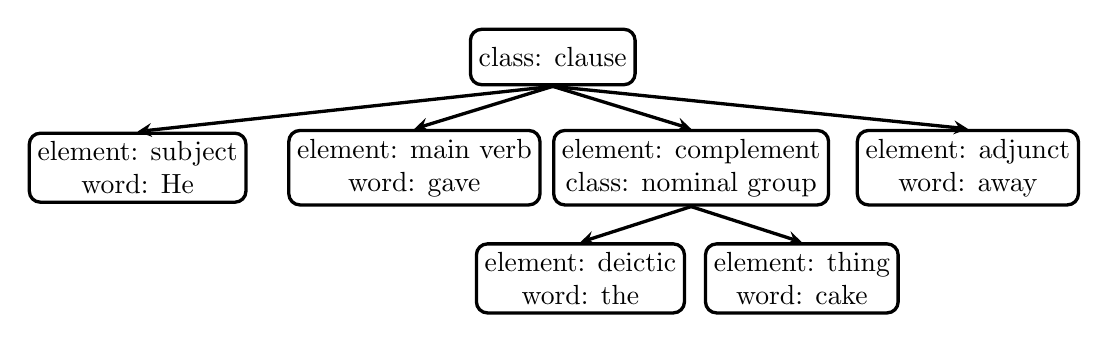
\begin{tikzpicture}[
    tree-style, 
%    edge-style,
    level 1/.style={sibling distance=10em},
    level 2/.style={sibling distance=8em},
    level distance = 4em
    ]
    \node[pattern-node]{class: clause}
    child {node[pattern-node]{element: subject\\word: He} }
    child {node[pattern-node]{element: main verb\\word: gave} }
    child {node[pattern-node]{element: complement\\class: nominal group}  {}
        child {node[pattern-node]{element: deictic\\word: the} }
        child {node[pattern-node]{element: thing\\word: cake} }
    }
    child {node[pattern-node]{element: adjunct\\word: away}  }
    ;
    \end{tikzpicture}
}
    \caption{Constituency graph corresponding to Example \ref{ex:transitivity1}}
    \label{fig:cg-transitive1}
\end{figure}
\begin{figure}[!ht]
\centering
\scalebox{0.7}{
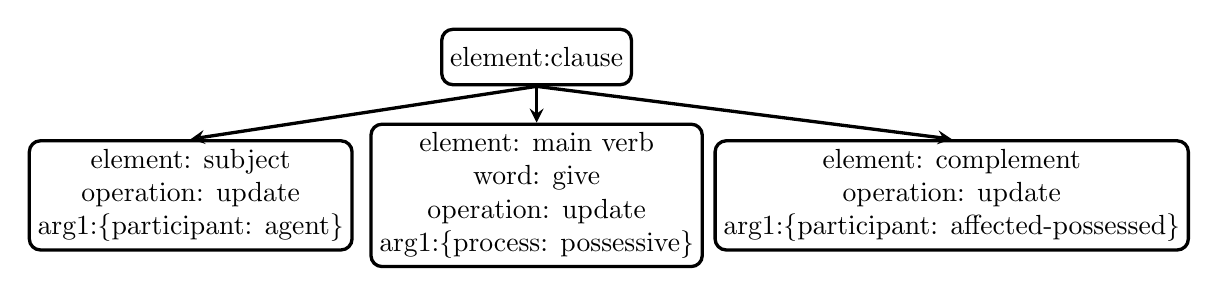
\begin{tikzpicture}[tree-style, level 1/.style={sibling distance=14em}, level distance = 5em]
\node[pattern-node]{element:clause}
	child {node[pattern-node, xshift=1.5em]{element: subject\\operation: update\\arg1:\{participant: agent\}} }
   	child {node[pattern-node]{element: main verb\\word: give\\operation: update\\arg1:\{process: possessive\}} }
    child {node[pattern-node, xshift=1em]{element: complement\\operation: update\\arg1:\{participant: affected-possessed\}}};
\end{tikzpicture}
}
\caption{A graph pattern for inserting agent and affected-possessed participant roles}
\label{fig:pg-transitive1}
\end{figure}
\begin{figure}[!ht]
    \centering
    \scalebox{0.7}{
        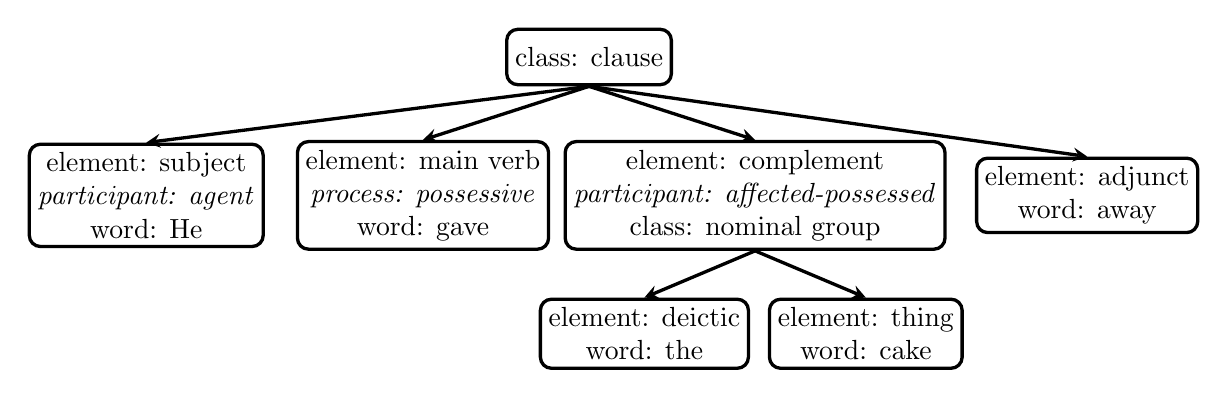
\begin{tikzpicture}[
        tree-style, 
        %    edge-style,
        level 1/.style={sibling distance=12em},
        level 2/.style={sibling distance=8em},
        level distance = 5em
        ]
        \node[pattern-node]{class: clause}
        child {node[pattern-node, xshift=2em]{element: subject\\\textit{participant: agent}\\word: He} }
        child {node[pattern-node]{element: main verb\\\textit{process: possessive}\\word: gave} }
        child {node[pattern-node]{element: complement\\\textit{participant: affected-possessed}\\class: nominal group}  {}
            child {node[pattern-node]{element: deictic\\word: the} }
            child {node[pattern-node]{element: thing\\word: cake} }
        }
        child {node[pattern-node]{element: adjunct\\word: away}  }
        ;
        \end{tikzpicture}
    }
    \caption{The resulting constituency graph enriched with participant roles}
    \label{fig:cgg-transitive1}
\end{figure}


Consider the same pattern, but applied to a sentence in the Table \ref{tab:di-transitive1}. 
The clause has two complements and they are by no means distinguished in the pattern graph. When such cases are encountered the PG yields two matches, (each with another complement) and the update operation is executed to both of the complements. To overcome such cases from happening PG allow defining \textit{negative nodes}, meaning that those are nodes that shall be missing in the target graph.

For example to solve previous case I define the PG depicted in figure \ref{fig:gp4} whose second complement is a negative node and it is marked with dashed line. This pattern is matched only against clauses with exactly one complement leaving aside the di-transitive ones because of the second complement.

\begin{table}[ht]
\centering
\begin{tabular}{|c|c|c|c|c|}
\hline
\multicolumn{5}{|c|}{class:clause}                                                                  \\ \hline
element:subject & element: main verb & element:complement & \multicolumn{2}{c|}{element:complement} \\ \hline
He              & gave               & her                & the               & cake.               \\ \hline
\end{tabular}
\caption{CG with a di-transitive verb}
\label{tab:di-transitive1}
\end{table}

\begin{figure}[hbtp]
\centering
\scalebox{0.8}{
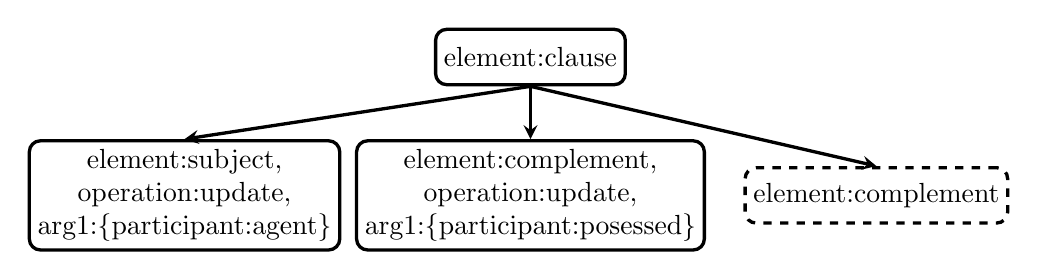
\begin{tikzpicture}[tree-style,level distance=5em, level 1/.style={sibling distance=12.5em},]
\node[pattern-node, anchor=center](vb1){element:clause}
	child {node[pattern-node,xshift=0em] {element:subject,\\operation:update,\\ arg1:\{participant:agent\}} edge from parent node[above] {}}
	child {node[pattern-node,xshift=0em] {element:complement,\\operation:update,\\ arg1:\{participant:posessed\}} edge from parent node[below right] {}}
	child {node[pattern-node-negative, xshift=0em] {element:complement} edge from parent node[above] {}};
\end{tikzpicture}
}
\caption{PG for inserting agent and possessed participant roles to subject and complement nodes only if there is no second complement.}
\label{fig:gp4}
\end{figure}

The current implementation of matching the patterns that contain negative nodes is performed in two steps. First the matching is performed with the PG without the negative nodes and in case of success another matching is attempted with the negative nodes included. If the second time the matching yields success then the whole matching process is unsuccessful but if the second phase fails then the whole matching process is successful because no configuration with negative nodes is detected.

For the sake of explanation I call the pattern graph with all the nodes (turned positive) \textit{big} and the pattern graph without the nodes marked negative \textit{small}. So then, matching a pattern with negative nodes means that matching the \textit{big} pattern (with negative nodes turned into positive) shall fail while matching the \textit{small} one (without the negative nodes) shall yield success.

%
\subsection{Pattern based node insertion} 
In English language there are cases when an constituent is missing because it is implied by the (grammatical) context. These are the cases of Null Elements treated in the Chapter \ref{ch:gbt}. 

\begin{exe}
	\ex\label{ex:albert} Albert asked [$\varnothing$ to go alone].
\end{exe}

Consider the Example \ref{ex:albert}. There are two clauses: first in which Albert asks something and the second where he goes alone. So it is Albert that goes alone, however it is not made explicit through a subject constituent in the second clause. Such implied elements are called \textit{null or empty constituents} discussed in detail in the Section \ref{sec:null-elements-gbt}. The table \ref{tab:Albert-example} provides a constituency analysis for the example and the null elements (in italic) are appended for the explicit grammatical account. In the Section \ref{sec:placing-null-elements} I offer the grammatical account of the graph patterns that insert these null elements into the parse graphs (so in fact extensively using the pattern based node insertion treated here).

\begin{table}[ht]
\centering
\begin{tabulary}{0.84\textwidth}{|C|C|C|C|C|C|}
\hline
\multicolumn{6}{|c|}{class:clause}                                                                                          \\ \hline
element: subject & element: main verb & \multicolumn{4}{c|}{element: complement, class:clause}                                \\ \cline{3-6} 
                &                    & \textit{element: subject}  & \multicolumn{2}{c|}{element: main verb} & element: adjunct \\ \hline
Albert          & asked              & \textit{Albert}           & to                 & go                & alone.          \\ \hline
\end{tabulary}
\caption{The constituency analysis that takes null elements into consideration}
\label{tab:Albert-example}
\end{table}

%\begin{figure}[hbtp]
%\centering
%%\includegraphics[width=0.8\textwidth]{figures/data-structures/dep-str-e11.png}
%\begin{dependency}[dep-style]
%	\begin{deptext}[]
%	NNP \& VBD \& TO \& VB \& RB \& . \\
%	Albert \& asked \& to \& go \& alone \& . \\
%	\end{deptext}
%\deproot{2}{root}
%\depedge{2}{1}{nsubj}
%\depedge{2}{4}{xcomp}
%\depedge{4}{3}{aux}
%\depedge{4}{5}{advmod}
%%\depedge[collage]{5}{6}{dobj}
%\end{dependency}
%\caption{Dependecy parse for ``Albert asked to go alone.''}
%\label{fig:ge3}
%\end{figure}

\begin{figure}[H]
\centering
\begin{tikzpicture}[tree-style,level distance=5em,] 
\node[pattern-node, anchor=center] (vb1){class:clause}
	child {node[pattern-node] (subj1) {element:subject,\\id:subj1}}
	child {node[pattern-node] (vb2) {element:complement,\\class:clause}
		child {node[pattern-node-negative] (subj2) {element:subject,\\operation:insert,\\arg1:\{id:subj1\}}}
	};
\end{tikzpicture}
\caption{A graph pattern to insert a reference node}
\label{fig:gp5}
\end{figure}

%explain the negated node
%explain the reference/clone vs brand new 

%The pattern that enables creation of reference node in subject position is illustrated in figure \ref{fig:gp5}. Note that the created node appears negated(or marked to be non-existent), this is to ensure that a subject does not already exist and avoid creating a clause with two subjects. 
To insert a new node the, PG needs to specify that (1) the inserted node does not already exist, so it is marked as negative node, (2) specify \textit{operation:insert} in the FS of the same and (3) provide id of the referenced node as FS argument (arg1) if one shall be taken.

In operational terms, the insertion operation means that the whole pattern will first go through a matching process. If there is a match then the new node is created. A peculiar thing about the created node is that it may keep a reference to another node or not. In our example it does keep a reference to the subject of dominant clause. If so, then all the features of the referee node are inherited by the new node. And if any are additionally provided then the new node overrides the inherited ones.

This section concludes our journey in the world of graph patterns, isomorphisms and graph based operations. Leaving only one more important data structure to cover: the system networks. 

\section{Systems and Systemic Networks}
\label{sec:system-networks-cs}
In the Section \ref{sec:system} I presented the basic definition of \textit{system} and \textit{system network} and the notations as formulated in the SF theory of grammar. In this work the system networks are simplified to hierarchies of disjoint features maintaining the entry conditions. This corresponds to the type logic component  described in \citep{ODonnell1993} where the syntagmatic organisation is restricted to a single functional layer. The reason behind this simplification is because the hierarchy of disjoint feature structures are perfectly suitable to correctly derive the complete set of parent features from a one or several manual selections. Moreover the systemic networks are not interconnected into an uniform grammar but separate modules describing selected aspects of language. Once the complete set of features is derived then it is associated with a graph pattern. This pattern graph is then used in the parse graph enrichment process described in Section \ref{sec:architecture}. Next I define the necessary concepts serving the current work.  

First I would like to introduce abstract concept of \textit{hierarchy} defined in a computer science fashion by \citet[30]{Pollard1987}  which is a formal rephrasing of Definition \ref{def:hierarchy} stating that the hierarchy is a sort of logical precedence among the terms of a system. 

\begin{definition}[Hierarchy]\label{def:hierarchy-cs}
	A hierarchy is finite bounded complete partial order $(\varDelta,\prec)$. 
\end{definition}

The next concept that requires closer formalization is that of a system first established in Definition \ref{def:system}. For precision purposes, this has a narrower scope without considering the system networks or precondition constraints; these are introduced shortly afterwards building upon current one.

\begin{definition}[System]\label{def:formal-system}
A \textit{system} $\Sigma=(l,P,C)$ labelled $l$ is defined by a finite disjoint set of distinct and mutually defining terms called a \textit{choice set} $C$ (of type $S_{XOR}$) and an \textit{entry condition set} $P$ (of type $S_{OR}$, $S_{XOR}$ or $S_{AND}$) establishing the delicacy relations within a system network.
%\begin{enumerate}
%	\item the choice set is a $S_{XOR}$ conjunction set.
%	\item the entry condition is a $S_{OR}$, $S_{XOR}$ or $S_{AND}$ conjunction set.
%%	\item \begin{equation*}
%%    \infty > size(C) \geq
%%	\begin{cases}
%%	2, & \text{if}\ T(C) = S_{XOR} \\
%%	3, & \text{if}\ T(C) = S_{OR} \\
%%	\end{cases}
%%	\end{equation*}
%\end{enumerate} 
\end{definition}

There is a set of functions defined that apply to systems: $label(\Sigma)=l$ is a function returning the system name, $choices(\Sigma)=C$ is a function returning the choice set, $precondition(\Sigma)=P$ is a function returning the set of entry condition features, and the $size(\Sigma)$ return the number of elements in the system choice set.  

\begin{definition}[Systemic delicacy]\label{def:delicacy-hierarchy}
	We say that a system $S_{1}$ is more delicate than $S_{2}$ denoted as $S_{1} \prec S_{2}$ if 
	\begin{enumerate}
		\item both system belong to the same system network: $S_{1}, S_{2} \in SN$ 
		\item there is at least a feature but not all of $S_{1}$ which belong to the entry condition of $S_{2}$ i.e. $choices(S_{1}) \in precondition(S_{2})$ or
        \item there is another system $S_{3}$ that has a among the entry conditions a feature of $S_1$ and whose features are among the entry conditions of $S_{2}$ i.e. $ \exists S'_{1} \in SN$ such that $ choices(S_{1}) \in precondition(S_{3}) \land choices(S'_{1}) \in precondition(S_{2})$
	\end{enumerate} 
\end{definition}

Systems are never used in isolation. SF grammars often are vast networks of interconnected systems defined as follows. 

%\begin{definition}[System Network]\label{def:system-network}
%	A \textit{system network} $SN=(r,SS)$ is defined as a hierarchy over a set of systems $SS$ where the order is that of systemic delicacy where:
%	\begin{enumerate}
%		\item $S_{i}$ is an arbitrary system within the hierarchy $S_{i} \in SS $
%		\item $r \in S_{i}$ is the unique root of the system network with empty precondition $precondition(r)=\varnothing $
%		\item $p_{i} = precondition(S_{i})$ the entry condition of system $S_{i}$.
%		\item $\tau: f \times S_{i} \rightarrow S_{j}$ a transition function from a feature $f \in precondition(S_{i})$ to a less delicate system $S_{j}, f \in choices(S_{j})$. We say that $S_{j} \prec S_{i}$
%	\end{enumerate}
%	subject to the following conditions:
%	\begin{enumerate}
%		\item $\forall x \in \cup \{ P_{i}| \forall P_{i} \in SN \}, \exists y \in \cup \{ choices(S_{i})| \forall S_{i} \in SN \}: x=y$ every precondition value is among the choice values
%		\item $\forall x \in \cup \{ P_{i}| \forall P_{i} \in SN \}$ there is a path $\pi$ (i.e. a sequence of systems) such that $\tau(x,\pi)=r$ (ensuring the connectedness of entire systemic network and a unique root)
%		\item $\nexists x \in \cup \{ P_{i}| \forall P_{i} \in SN \}$ and $\nexists \pi$ such that $\exists S_{j}=\tau(x,\pi)$ and that $ S_{j} \in \pi \vee x \in values(S_{j}) $ (ensuring the system network is no cyclical)
%	\end{enumerate}
%\end{definition}

\begin{definition}[System Network]\label{def:system-network}
    A \textit{system network} $SN=(r,\Gamma)$ is defined as a hierarchy over a set of systems $\Gamma$ where the order is that of systemic delicacy starting from a root feature $r$ such that for any system in the network either there is another less delicate system or its entry condition is the root feature i.e. \mbox{$\forall S_{i} \in \Gamma, \exists S_{j} \in \Gamma | S_{j} \prec S_{i} \lor precondition(S_{i})=r$}. 
\end{definition}

%%TODO: define realisation statements
%So far we have defined what system networks are but an important element has been omitted - the realisation statements. Robin Fawcett always stated that there are ``no system networks without realisation statements''. They are associated with system features and indicate what operations need to be executed in order to instantiate that feature. The current work does not deal with the generation task but with parsing and a part of this task is recognition whether the premises of the feature are already in structure and if so then assign the feature to the structure. By the premisses of a feature I mean the graph pattern that is necessary and sufficient to realise a feature.    In this work the equivalent of the realisation statement are pattern graphs. These aspects are further discussed in Section \ref{sec:system-network-execution} dealing with the execution of system networks.  

%Now you may ask a pertinent question: what is the basis on which is the systemic selection made? To answer it I must first introduce two types of constraints. First, The systems are interconnected with each other by a set of preselection (entry) conditions forming systemic networks (Definition \ref{def:system-network}). Second, is an aspect not always mentioned in the SFL literature, the systemic \textit{realisation statements} which are shaping the context where the system is applied. These aspects are covered in Section \ref{sec:system-network-execution} talking about execution of system networks.  

%The graphical notation of system networks has been introduced in Section \ref{sec:system}. The notation for writing system networks from \citep{Halliday2013} is more appropriate for explaining concepts such as \textit{selection path} and \textit{feature network} that follows next. This compressed notation for writing system networks uses colon (:) to symbolize entry condition leading to terms in systems, slash (/) for systemic contrast (disjunction) and ampersand (\&) for systemic combination (conjunction). So a sample network will be written as follows:
%
%\begin{exe}
%	\ex\label{ex:system10} $\varnothing: i_1 / i_2/i_3 $
%	\ex\label{ex:system11} $i_1: i_4 / i_5 $
%	\ex\label{ex:system12} $i_2$ \& $i_4: i_6 / i_7 $
%\end{exe}
%
%However in this thesis we need to account for the disjunction type and system name. So we adopt a slightly different notation of three slots separated by colon (:) where the first slot signifies the system name, second the set of system features and the third is the entry condition. Examples \ref{ex:system1} to \ref{ex:system3} show three systems definitions (without selection functions i.e. no realization statements). 
%\begin{exe}
%	\ex\label{ex:system1} $S_1:OR(i_1,i_2,i_3):\varnothing$
%	\ex\label{ex:system2} $S_2:XOR(i_4,i_5):OR(i_1)$
%	\ex\label{ex:system3} $S_3:XOR(i_6,i_7):AND(i_2,i_4)$
%\end{exe}

In a systemic network $SN$ where a system $S_l$ depends on the choices in another system $S_e$ (i.e. the preconditions of $S_l$ are features of $S_e$) we call the $S_e$ an \textit{early(older) system} and the $S_l$ a \textit{late(younger) system}. This is just another way to refer to order systems according to their delicacy but applying this ordering to execution of systemic selection. 

The graphical notation of system networks has been introduced in Section \ref{sec:system}. Considering the above definitions, the system network can be represented as a graph where each node is a system features and edges represent precondition dependencies. Figure \ref{fig:system-network-example0} depicts examples of a system network with three systems. In Figure \ref{fig:system-network-example1} the entry conditions are $S_AND$ sets only and in Figure \ref{fig:system-network-example2} the entry condition for $S_3$ is $OR(f_2,f_4)$ depicted with dashed lines. In such a graph, all system features must be unique i.e. ${\forall S_1, S_2 \in SN: choices(S_1) \cap choices(S_2) = \varnothing}$ and there must be no dependency loops.

\begin{figure}[!ht]
	\centering
    \begin{subfigure}[t]{0.47\textwidth}
        \centering
        \scalebox{0.7}{
            \begin{tikzpicture}[scale=0.8]
            \tikzstyle{system-features}=[rectangle, draw=black, rounded corners, text centered, anchor=west, rectangle split, thick]
            \tikzstyle{system-name}=[rectangle, draw=none, thick, text centered]
            \tikzstyle{precondition} = [->, thick, black]
            
            \node (s1n) [system-name] {$S_1$};
            \node (s1b) [system-features, rectangle split parts=4, right =0em of s1n.north east, anchor=north west]
            {XOR  
                \nodepart{second}
                $f_1$ \nodepart{third}
                $f_2$ \nodepart{fourth}
                $f_3$};
            \node (es) [system-name, left = 2em of s1n] {$\varnothing$};
            \draw[precondition] (s1n.west) -- (es.east);
            
            \node (s2n) [system-name, above right = 4em of s1b.north,xshift = 1em] {$S_2$};
            \node (s2b) [system-features, rectangle split parts=3, right=0em of s2n.north east, anchor=north west]
            {XOR  
                \nodepart{second}$f_4$
                \nodepart{third}$f_5$};
            %	\draw[black, thick] (s2n.south) -- (s2b.west);
            
            \node (s3n) [system-name, below right = 4em of s2b.south, xshift = 2em] {$S_3$};
            \node (s3b) [system-features, rectangle split parts=3, right =0em of s3n.north east, anchor=north west]
            {XOR  
                \nodepart{second}$f_6$
                \nodepart{third}$f_7$};
            %	\draw[black, thick] (s3n.south) -- (s3b.west);
            
            \draw[precondition] (s3n.west) -- ([xshift=0em,yshift=0em] s2b.east);
            \draw[precondition] (s3n.west) -- ([xshift=0em,yshift=-0.8em] s1b.east);
            \draw[precondition] (s2n.south) -- ([xshift=0em,yshift=0.5em] s1b.east);
            
            \end{tikzpicture}
        }
        \caption{System Network with conjunctive entry conditions}
        \label{fig:system-network-example1}
    \end{subfigure} 
    \begin{subfigure}[t]{0.47\textwidth}
    \centering
    \scalebox{0.7}{
        \begin{tikzpicture}[scale=0.8]
        \tikzstyle{system-features}=[rectangle, draw=black, rounded corners, text centered, anchor=west, rectangle split, thick]
        \tikzstyle{system-name}=[rectangle, draw=none, thick, text centered]
        \tikzstyle{precondition} = [->, thick, black]
        
        \node (s1n) [system-name] {$S_1$};
        \node (s1b) [system-features, rectangle split parts=4, right =0em of s1n.north east, anchor=north west]
        {XOR  
            \nodepart{second}
            $f_1$ \nodepart{third}
            $f_2$ \nodepart{fourth}
            $f_3$};
        \node (es) [system-name, left = 2em of s1n] {$\varnothing$};
        \draw[precondition] (s1n.west) -- (es.east);
        
        \node (s2n) [system-name, above right = 4em of s1b.north,xshift = 1em] {$S_2$};
        \node (s2b) [system-features, rectangle split parts=3, right=0em of s2n.north east, anchor=north west]
        {XOR  
            \nodepart{second}$f_4$
            \nodepart{third}$f_5$};
        %	\draw[black, thick] (s2n.south) -- (s2b.west);
        
        \node (s3n) [system-name, below right = 4em of s2b.south, xshift = 2em] {$S_3$};
        \node (s3b) [system-features, rectangle split parts=3, right =0em of s3n.north east, anchor=north west]
        {XOR  
            \nodepart{second}$f_6$
            \nodepart{third}$f_7$};
        %	\draw[black, thick] (s3n.south) -- (s3b.west);
        
        \draw[precondition, dashed] (s3n.west) -- ([xshift=0em,yshift=0em] s2b.east);
        \draw[precondition, dashed] (s3n.west) -- ([xshift=0em,yshift=-0.8em] s1b.east);
        \draw[precondition] (s2n.south) -- ([xshift=0em,yshift=0.5em] s1b.east);
        \end{tikzpicture}
    }
    \caption{System Network with disjunctive entry condition for $S_3$}
    \label{fig:system-network-example2}
\end{subfigure}

	\caption{Example System Network presented as graphs}
    \label{fig:system-network-example0}
\end{figure}

%%TODO introduce a realistic example 

For a chosen feature in the system network it is possible to trace a path to the root feature by traversing systems through their preconditions. Generating such a path is equivalent to preselecting the features in all earlier systems. This is needed for assigning a complete set of feature selections to a pattern graph before it is used in the parse graph enrichment. Conversely, in the verification process it is necessary to check whether a set of arbitrary features belong to a \textit{consistent} and \textit{complete selection path}. Next are addressed the concepts needed for addressing this task and how it is executed.

The system networks from Figure \ref{fig:system-network-example0} can be unpacked into a \textit{feature network} (Definition \ref{def:maximal-selection-graph} which is referred to as \textit{maximal selection graph}) interconnected by system entry conditions. In Figure \ref{fig:feature-network-example0} are depicted two feature networks corresponding to the system networks above. The dashed lines mean disjunction and continuous ones mean conjunction of entry features. 

\begin{figure}[!ht]
    \centering
    \begin{subfigure}[t]{0.47\textwidth}
        \centering
        \scalebox{0.95}{
            \begin{tikzpicture}[scale=1]
               	\tikzstyle{system-features}=[rectangle, draw=black, rounded corners, text centered, thick]
                \tikzstyle{system-name}=[rectangle, draw=none, thick, text centered]
                \tikzstyle{precondition} = [->, thick, black]
                
                \node (i1) [system-features] {$i_1$};
                \node (i2) [system-features, below =1em of i1] {$i_2$};
                \node (i3) [system-features, below =1em of i2] {$i_3$};
                
                \node (i4) [system-features, above right =5em of i2] {$i_5$};
                \node (i5) [system-features, below =1em of i4] {$i_4$};
                
                \node (i6) [system-features, below right=5em of i4] {$i_6$};
                \node (i7) [system-features, below =1em of i6] {$i_7$};
                
                \draw[precondition] ([xshift=-0.1em] i5.west) -- ([xshift=0.3em,yshift=-0.2em] i1.east);
                \draw[precondition] ([xshift=-0.1em] i4.west) -- ([xshift=0.3em,yshift=0.1em] i1.east);
                \draw[precondition] ([xshift=-0.1em] i6.west) -- ([xshift=0.3em,yshift=0.1em] i5.east);
                \draw[precondition] ([xshift=-0.1em] i7.west) -- ([xshift=0.3em,yshift=-0.3em] i5.east);
                \draw[precondition] ([xshift=-0.1em] i6.west) -- ([xshift=0.3em,yshift=0.2em] i2.east);
                \draw[precondition] ([xshift=-0.1em] i7.west) -- ([xshift=0.3em,yshift=-0.2em] i2.east);
            \end{tikzpicture}
        }
        \caption{Feature Network graph with conjunctive entry conditions only}
        \label{fig:feature-network-example1}
    \end{subfigure} 
    \begin{subfigure}[t]{0.47\textwidth}
        \centering
        \scalebox{0.95}{
            \begin{tikzpicture}[scale=1]
               	\tikzstyle{system-features}=[rectangle, draw=black, rounded corners, text centered, thick]
                \tikzstyle{system-name}=[rectangle, draw=none, thick, text centered]
                \tikzstyle{precondition} = [->, thick, black]
                
                \node (i1) [system-features] {$i_1$};
                \node (i2) [system-features, below =1em of i1] {$i_2$};
                \node (i3) [system-features, below =1em of i2] {$i_3$};
                
                \node (i4) [system-features, above right =5em of i2] {$i_5$};
                \node (i5) [system-features, below =1em of i4] {$i_4$};
                
                \node (i6) [system-features, below right=5em of i4] {$i_6$};
                \node (i7) [system-features, below =1em of i6] {$i_7$};
                
                \draw[precondition] ([xshift=-0.1em] i5.west) -- ([xshift=0.3em,yshift=-0.2em] i1.east);
                \draw[precondition] ([xshift=-0.1em] i4.west) -- ([xshift=0.3em,yshift=0.1em] i1.east);
                \draw[precondition, dashed] ([xshift=-0.1em] i6.west) -- ([xshift=0.3em,yshift=0.1em] i5.east);
                \draw[precondition, dashed] ([xshift=-0.1em] i7.west) -- ([xshift=0.3em,yshift=-0.3em] i5.east);
                \draw[precondition, dashed] ([xshift=-0.1em] i6.west) -- ([xshift=0.3em,yshift=0.2em] i2.east);
                \draw[precondition, dashed] ([xshift=-0.1em] i7.west) -- ([xshift=0.3em,yshift=-0.2em] i2.east);
            \end{tikzpicture}
        }
        \caption{Feature Network graph with some disjunctive entry condition}
        \label{fig:feature-network-example2}
    \end{subfigure}
    
    \caption{Example Feature Network graphs}
    \label{fig:feature-network-example0}
\end{figure}

The feature network can be defined in relation to the system network as follows.

\begin{definition}[Feature Network]\label{def:maximal-selection-graph}
For a given system network $SN=(r,\Gamma)$, a \textit{Feature Network} $FN(N,E)$ is a directed graph whose nodes $N$ are the union of choice sets of the systems $\Gamma$ and the edges $E$ connect choice features with the entry condition (precondition) features of the systems $\Gamma$. 
%Formally it can be expressed as follows: 
%\begin{enumerate}
%	\item $N = \bigcup choices(\Sigma_{i})$ where $\Sigma_{i} \in SN$ for $0 < i size(SN)$
%	\item $E = \{(f_{m},f_{n})\}$ where $f_{m} \in  choices(\Sigma_{i}), f_{n} \in precondition(\Sigma_{i})$
%\end{enumerate}
\end{definition}
%eventually offer a formal description of edges and nodes

%The Feature Network in fact is an expansion of the System Network. The former is a network of interconnected features while the latter a network of systems. 

%\begin{definition}[Selection Path]\label{def:selection-path}
Given a feature network $FN(N,E)$ and a feature the network $f \in N$ a \textit{selection path} $SP(N,E)$ is a connected sub-graph of traversal paths between the root of the feature network and the feature $f$. A \textit{complete selection path} is a selection path from one of the leaf nodes up to the network root. 
%\end{definition}

\begin{figure}[!ht]
    \centering
    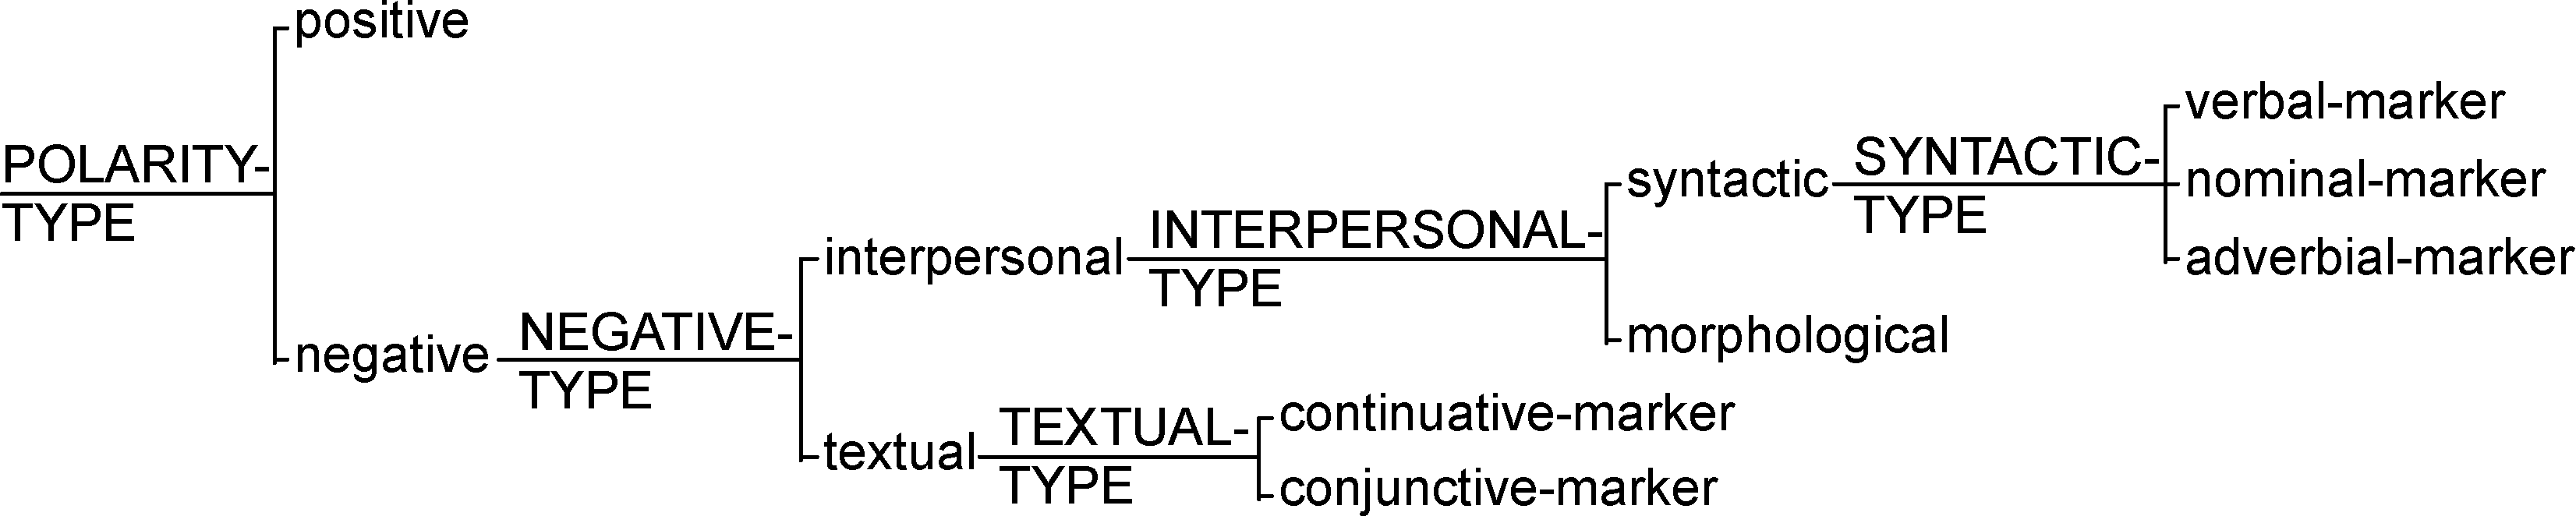
\includegraphics[width=\textwidth]{Figures/SFL-grammar/polarity-system.pdf}
    \caption{Polarity System}
    \label{fig:polarity1}
\end{figure}

%The process of creating selection path is sometimes called \textit{system network instantiation}. 
The selection path is generated by traversal of the feature network from a given feature node towards the rood node. If the node has no incoming edge then the result traversal it is a leaf node and the resulting selection path is a complete one. For example if \textit{verbal-marker} feature is selected in the system network depicted in Figure \ref{fig:polarity1} the traversal of the corresponding feature network towards root feature yields the selection path \textit{negative -- interpersonal -- syntactic -- verbal-marker}. This path is also complete with respect to the network because there are no systems younger than the SYNTACTIC-TYPE system.

When the system networks define more than one feature in the precondition it leads to split paths it means that there is more than one feature needs to or can be preselected. If the edge is a continuous line (depicted  in Figure \ref{fig:feature-network-example1}) the both variants are part of the same selection path. In case the edge is a dashed line (depicted  in Figure \ref{fig:feature-network-example2}) the paths are considered alternative and further decision making mechanism shall be employed to reduce the disjunction to a single variant. In the current work no such mechanism is employed and the parse result is presented with both alternatives. In most cases the entry condition is constituted of a single feature, when there are multiple ones, usually they are conjuncted and only in a small minority of cases entry condition is a disjunction of features.

\begin{algorithm}[!ht]
    \Input {\feature, \snet}
    \Begin {
        add \feature to empty selection path \;
        \For{\systemm \KwTo traversal path to the root of \snet}
        {
            get entry condition features of \systemm \;
            add entry condition features to the selection path \;
        }
        \Return{selection path}
    }
    \caption{Naive backwards induction of a selection path}
    \label{alg:backward-induction-naive}
\end{algorithm}

The pseudo code for creating a selection path as described above is outlined in Algorithm \ref{alg:backward-induction-naive}. Given a system network a random non root feature belonging to the network, it traverses the networks, one by one, towards the root and collects the entry conditions of each system into a selection path.

\section{On realisation rules}
\label{sec:realisation-reules}
The previous section explains that in the current work systemic networks are simplified to a taxonomy of features and no realisation rules are considered. This section explains how the pattern graphs are a substitute to the realisation rules and how they relate to each other.

The \textit{realisation rule} of a systemic feature specifies how that feature is realised as a syntagmatic structure down to a text form using operations such as insert or expand constituent, order two constituent, preselect another feature, lexicalise etc. They are the essential ingredient binding the paradigmatic description into a syntagmatic structure.
Robin Fawcett recurrently emphasises the role of realization rules in the composition of system networks. He often stresses ``no system networks without realization rules''.  
It is the \textit{instantiation} process that in Halliday's words ``is the relation between a semiotic system and the \textit{observable} events or `acts' of meaning'' \citep[emphasis added]{Halliday2003-systemic-theory}. The realisation rules for a systemic feature are the statement of operations through which that feature contributes to the structural configuration (that is being either generated or recognised) \citep[p.86]{Fawcett2000}.

It is not easy however for linguists and grammarians to provide such statements for the systemic features. Doing so means an explicit formalisation of grammar on top of charting the systemic composition and dependencies which is already a challenging task in its own. Not to mention that writing a good grammar is already a very difficult task. The realisation rules most of the time remain in the minds of the interpreters who can recognise a feature when it occurs. Adding the formal specification of the realisation rule requires tools for consistency checking with respect to the rest of the grammar and large corpus query tool to test various rule hypotheses which are not really available yet. 

%The graph patterns described in this chapter can be a suitable approach to address the problem of missing realisation rules.

In this work the graph patterns can be considered as bundles of realisation rules and feature selections and therefore an approach to replace the realisation rules. This idea is implicitly covered in Section \ref{sec:pattern-graphs} and here I explicitly describe it through an example. Consider the fragment of the Mood system network from \citet[162]{Halliday2013} depicted in Figure \ref{fig:mood-fragment}. This example aims at three feature selections: major, indicative and declarative. The root feature in the system network is realised through a constituent \textit{clause}, any of the selected fratures is ascribed directly to it, and the selection of any subsequent features impacts the elements below through the associated realisation rules. The pattern graph that captures selection of major feature is depicted in Figure \ref{fig:mood-fragment-major}. 

\begin{figure}[!ht]
    \centering
    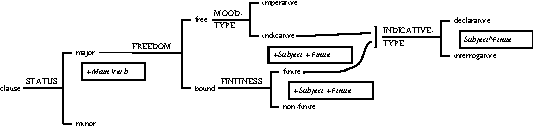
\includegraphics[width=\textwidth]{Figures/Example/mood-fragment.pdf}
    \caption{An adapted fragment of a Mood system from \citep[162]{Halliday2013} }
    \label{fig:mood-fragment}
\end{figure}

\begin{figure}[!ht]
    \centering
    \scalebox{0.7}{
    \begin{tikzpicture}[tree-style,level distance=5em,] 
    \node[pattern-node, anchor=center] (c) {class:clause, STATUS:major}
    child {node[pattern-node] (subj1) {element:Main Verb}};
    \end{tikzpicture}
    }
    \caption{A graph pattern for \textit{major} feature selection in Figure \ref{fig:mood-fragment}}
    \label{fig:mood-fragment-major}
\end{figure}

In Figure \ref{fig:mood-fragment-indicative} is depicted the pattern graph corresponding to the selection of indicative feature. Here the clause constituent receives the whole selection path up to the root feature \textit{clause -- major -- free -- indicative} and in addition two more constituents are required: Subject and Finite. Almost same pattern graph is valid in case of selecting bound feature instead of indicative.

\begin{figure}[!ht]
    \centering
    \scalebox{0.7}{
    \begin{tikzpicture}[tree-style,level distance=5em,] 
    \node[pattern-node, anchor=center] (c) {class:clause, STATUS:major, FREEDOM:free,\\MOOD-TYPE:indicative }
    child {node[pattern-node] (subj1) {element:Main Verb}}
    child {node[pattern-node] (subj1) {element:Subject}}
    child {node[pattern-node] (subj1) {element:Finite}}
    ;
    \end{tikzpicture}
    }
    \caption{A graph pattern for \textit{indicative} feature selection in Figure \ref{fig:mood-fragment}}
    \label{fig:mood-fragment-indicative}
\end{figure}

\begin{figure}[!ht]
    \centering
    \scalebox{0.7}{
    \begin{tikzpicture}[tree-style,level distance=5em,] 
    \node[pattern-node, anchor=center] (c) {class:clause, STATUS:major, FREEDOM:free,\\ MOOD-TYPE:indicative, INDICATIVE-TYPE:declarative }
    child {node[pattern-node] (subj1) {element:Main Verb}}
    child {node[pattern-node] (subj1) {element:Subject,\\precede:fnt}}
    child {node[pattern-node] (subj1) {id:fnt,\\element:Finite}}
    ;
    \end{tikzpicture}
    }
    \caption{A graph pattern for \textit{declarative} feature selection in Figure \ref{fig:mood-fragment}}
    \label{fig:mood-fragment-declarative}
\end{figure}

In Figure \ref{fig:mood-fragment-declarative} the selection is taken one step further to the declarative feature. The associated realisation rule is ordering the Subject and Finite elements. This is captured via the ``precede:fnt'' where ``fnt'' is the id of the Finite constituent. 

\begin{figure}[!ht]
    \centering
    \scalebox{0.7}{
    \begin{tikzpicture}[tree-style,level distance=5em,] 
    \node[pattern-node, anchor=center] (c) {MOOD-TYPE:indicative, INDICATIVE-TYPE:declarative }
    child {node[pattern-node] (subj1) {element:Subject,\\precede:fnt}}
    child {node[pattern-node] (subj1) {id:fnt,\\element:Finite}}
    ;
    \end{tikzpicture}
    }
    \caption{A graph pattern for the selection if \textit{indicative} and \textit{declarative} features in Figure \ref{fig:mood-fragment}}
    \label{fig:mood-fragment-declarative-indicative-isolated}
\end{figure}

The pattern does not need to refer to the complete selection path but can be limited to the context of a few related features. For example to represent selection of indicative and declarative features in isolation is depicted in Figure \ref{fig:mood-fragment-declarative-indicative-isolated}. In this case the class of the parent constituent (that in the above cases is the clause) is no longer specified because the restricted selection path and thus the root of the network is not reached. Also none of the preselected features major and free are specified either.  

One limitation, however, of the graph patterns is dealing with conflation phenomena. For example, the cases of the Main Verb conflated with Finite elements have to be accounted by with pattern graphs where one constituent has two functions instead of pattern graphs with two separate constituent each with the corresponding function. This limitation can be addressed in the future by manipulating the definition of the feature structure matcher described in Section \ref{sec:graph-matching}.

\section{Discussion}
This chapter described from a computer science perspective the SFL concepts introduced in Chapter \ref{ch:sfg} and prepares the ground for the following chapters that address the implementation details of the Parsimonious Vole parser.  

A central theme covered here are the graphs and graph patterns. They play the key role in identifying grammatical features in dependency and constituency structures. They are also an excellent candidate for expressing \textit{systemic realizations} which have not been considered in the current work as being associated to the systemic features.  

In Section \ref{sec:realisation-reules} I mentioned that authoring realisation rules is a difficult task and requires a proper tool support. The same is the case for graph patterns and even more so when they need to be related to systemic networks or network parts. The system network authoring tool, such as the one available in UAM Corpus Tool \citep{ODonnell2008a}, should provide also a graph pattern editor allowing association of graph patterns to systemic features. Unfortunately building such an editor is out of the scope of the current work and is among the priorities in the future developments. Also employing a mature specialised technology for manipulating large amounts of graph data available in the Semantic Web suite of tools is another direction for the future described in the Section \ref{sec:future-work}.

In the next chapter I describe the parsing pipeline and how each step is implemented starting from Stanford dependency graph all the way down to a rich constituency systemic functional parse structure.

%copied
%Robin Fawcett recurrently emphasises the role of realization rules in the composition of system networks. He often stresses ``no system networks without realization rules''. They are important because they formally express ways in which a feature is identified or realised. It is the \textit{instantiation} process that in Halliday's words ``is the relation between a semiotic system and the \textit{observable} events or `acts' of meaning'' \citep[emphasis added]{Halliday2003-systemic-theory}. The realisation rules for a systemic feature are the statement of operations through which that feature contributes to the structural configuration (that is being either generated or recognised) \citep[p.86]{Fawcett2000}.

%It is not easy however for linguists and grammarians to provide such statements for the systemic features. Doing so means an explicit formalisation of grammar on top of charting the systemic composition and dependencies which is already a challenging task in its own. The realisation rules most of the time remain in the minds of the interpreters who can recognise a feature when it occurs. Adding the formal specification of the realisation rule requires tools for consistency checking with respect to the rest of the grammar and large corpus query tool to test various rule hypotheses. 

%Moreover the expression of rules is proposed in terms of atomic operations such as lexify, preselect, insert, order, etc. Which may not always be fully transparent to the grammarian. Expressing realization rules as operations contextualised in fragments of parse structure is a promising way to ease the grammar authoring process. They could then be used directly by the parser to recognise such structures making the corpus annotation and grammar construction an in-parallel evolving process.

%The data structures and operations with them described in this chapter can be a suitable approach to address the problem of missing realisation rules from the system networks.
%To do so however requires creation of a system network authoring tool (such as the one available in UAM Corpus Tool \citep{ODonnell2008a}) which besides systemic network editor should contain also a graph pattern editor allowing association of graph patterns to systemic features. 

%In current parser the pattern graphs are represented as compositions of Python dictionaries and lists such as the one below.
%%* The Patterns are written as python data structures thus not very user friendly, an editor would be much more helpful
%\begin{Verbatim}[fontsize=\relsize{-2}]
%{
%    NODES: {  
%        "cl": [
%            {C_TYPE: 'clause', 
%             VOICE: ACTIVE},
%            {CONFIGURATION: ['two-role-action', ['Ag', 'Ra', 'Cre']], }],
%        'pred': [
%            {C_TYPE: [PREDICATOR, PREDICATOR_FINITE], }, 
%            {VERB_TYPE: "main", PROCESS_TYPE: 'two-role-action'} ],
%        'subj': [
%            {C_TYPE: SUBJECT, }, 
%            {PARTICIPANT_ROLE: 'Ag'}],
%        'compl1': [
%            {C_TYPE: [COMPLEMENT, COMPLEMENT_DATIVE], },
%            {PARTICIPANT_ROLE: 'Ra'}],
%        'compl2': [
%            {C_TYPE: [COMPLEMENT, COMPLEMENT_ADJUNCT, ], },
%            {PARTICIPANT_ROLE: 'Cre'}],
%    },
%    EDGES: [
%    ['cl', 'pred', None], 
%    ['cl', 'subj', None], 
%    ['cl', 'compl1', None], 
%    ['cl', 'compl2', None],]
%}
%\end{Verbatim}
%
%This Python dictionary contains two top keys: NODES defined as  with node identifiers each associated with a set of systemic features and EDGES defined as a list with three tuples of source, target and eventually a dictionary of features. The nodes contain a list of two dictionaries. The first dictionary enlists the features that the backbone structure should already carry, and against which the pattern matching is performed. The second dictionary contains the set of features that the node shall receive in case of a successful match of the entire pattern. 

%Writing such structures is cumbersome and requires in depth knowledge of the parser and employed system networks therefore the need for an editor is even higher. 
%Unfortunately building such an editor is out of the scope of the current work and is among the priorities in the future developments just as switching to better technology for working with graphs such as Semantic Web suite of tools. This and other future work are described in the Section \ref{sec:future-work}.
%
%In the next chapter I describe the parsing pipeline and how each step is implemented starting from Stanford dependency graph all the way down to a rich constituency systemic functional parse structure.
% \chapter{Creating the systemic functional constituency structure}
\label{ch:parsing-algorithm}

    The previous chapter introduced the building blocks for the parser pipeline algorithm depicted in Figure \ref{fig:pipeline-overview}. This chapter covers the entire first phase of the algorithm called ``graph building''. The input for the parsing pipeline is made up of Stanford dependency parse graphs. The dependency graphs are sometimes erroneous or treat certain linguistic phenomena in a way incompatible with current approach. Therefore a preprocessing stage is needed to correct and canonicalise the dependency graphs; this is covered in Sections \ref{sec:preprocessing1} and \ref{sec:preprocessing2}. Then these graphs are rewritten into systemic constituency graphs. The process by which this happens is covered in Section \ref{sec:creation-constituency-graph}.

\section{Canonicalisation of dependency graphs}
\label{sec:preprocessing1}
    Beside stable errors, there are two other phenomena that are modified in the preprocessing phase: \textit{copula} and \textit{coordination}. They are not errors per se but represent simply an incompatibility between how the Stanford parser represents them and how they need to be represented for processing by the current algorithm and grammar.

    In this section I describe a set of transformation operations on the dependency graph before it is transformed into a systemic constituency graph. The role of the preprocessing phase is to bring in line aspects of the dependency parse to a form compatible with the systemic constituency graph creation process by (a) correcting known errors in DG, (b) cutting down some DG edges to form a tree, and (c) changing the Stanford parser's standard handling of copulas, coordination and few other phenomena. This is achieved via three transformation types: (a) \textit{relabelling of edge relations}, (b) relabelling node POS, and (c) reattachment of nodes to a different parent. 

\subsection{Loosening conjunction edges}
    The Stanford parser employs an extra edge for each of the conjuncts such that there is one indicating the syntactic relationship to the child or parent nodes (just like for any other nodes) and additionally one that shows the conjunction relationship to its sibling nodes. In this step, the parent or child relations except for the first conjunct are removed leaving only the sibling relations. 

    Some common patterns occurring between noun, verb and adjective conjuncts are depicted in Figures \ref{fig:conj-noun} - \ref{fig:conj-verb-subj}.

    \begin{figure}[!ht]
    \centering
        \begin{subfigure}[b]{0.45\textwidth}
        \centering
        \resizebox{0.97\textwidth}{!}{%
        	\begin{dependency}[dep-style]
        		\begin{deptext}[]
        	Cats \& and \& dogs \& can \& be \& friends \& . \\ 
        		\end{deptext}
        	%	\deproot{3}{root}
        	%	\depedge{3}{1}{aux}
        	%	\depedge{3}{2}{nsubj}
        	%	\depedge{3}{4}{iobj}
        	%	\depedge{6}{5}{det}
        		\depedge{6}{1}{nsubj}
        		\depedge{6}{3}{nsubj}	
        		\depedge{1}{3}{conj\_and}
        	\end{dependency}
        	}
            \caption{Composite subject}
            \label{fig:conj-noun-subj}
        \end{subfigure}%
        \quad
        \begin{subfigure}[b]{0.45\textwidth}
            \centering
            \resizebox{0.97\textwidth}{!}{%
        	\begin{dependency}[dep-style]
        		\begin{deptext}[]
        	Please \& give \& me \& a \& fork \& and \& a \& knife \\ 
        		\end{deptext}
        	%	\deproot{3}{root}
        	%	\depedge{3}{1}{aux}
        	%	\depedge{3}{2}{nsubj}
        	%	\depedge{3}{4}{iobj}
        	%	\depedge{6}{5}{det}
        		\depedge{3}{6}{dobj}
        		\depedge{3}{8}{dobj}	
        		\depedge{6}{8}{conj\_and}
        	\end{dependency}
        	}
            \caption{Composite object}
            \label{fig:conj-noun-obj}
        \end{subfigure}
        \caption{Conjunction of nouns in subject and object positions}
        \label{fig:conj-noun}
    \end{figure}


    \begin{figure}
    \centering
    \begin{dependency}[dep-style]
    		\begin{deptext}[]
    	It \& is \& hard \& for \& both \& me \& and \& you \& . \\ % \& , \& makes \& ... \\
    		\end{deptext}
    		%\deproot{3}{root}
    		%\depedge{3}{1}{expl}
    		%\depedge{3}{2}{cop}
    		%\depedge{6}{5}{preconj}
    		\depedge{3}{6}{prep\_for}
    		\depedge{3}{8}{prep\_for}
    		\depedge{6}{8}{conj\_and}
    	\end{dependency}
    \caption{Conjunction of prepositional phrases}
    \label{fig:conj-preps}
    \end{figure}

    \begin{figure}[!ht]
    \centering
    	\begin{dependency}[dep-style]
    		\begin{deptext}[]
    	He \& is \& strong \& and \& brave \& . \\
    		\end{deptext}
    		%\deproot{3}{root}
    		\depedge{3}{1}{nsubj}
    		\depedge{5}{1}{nsubj}
    		%\depedge{3}{2}{cop}
    		\depedge{3}{5}{conj\_and}
    	\end{dependency}
    \caption{Conjunction of copulatives sharing the subject}
    \label{fig:conj-copula-subj}
    \end{figure}


    \begin{figure}[!ht]
    \centering
    	\begin{dependency}[dep-style]
    		\begin{deptext}[]
    	He \& came \& home \& and \& immediately \& washed \& his \& hands \& . \\ 
    		\end{deptext}
    		%\deproot{2}{root}
    		\depedge{2}{1}{nsubj}
    		\depedge{6}{1}{nsubj}
    		%\depedge{2}{3}{dobj}
    		\depedge{2}{6}{conj\_and}
    		%\depedge{6}{5}{advmod}
    		%\depedge{8}{7}{poss}
    		%\depedge{6}{8}{dobj}
    	\end{dependency}
    \caption{Conjunction of verbs sharing the same subject}
    \label{fig:conj-verb-subj}
    \end{figure}

    The main reason these extra edges need to be removed is to avoid traversal of the same node via different paths. This, in the current algorithm, has as consequence execution of the same operation multiple times such as for example creation of multiple constituents from the same DG node, which is of course undesirable. For example, if multiple subject relations occur in the DG then multiple subjects are going to be instantiated in CG and this is grammatically incorrect. Rather only one complex unit needs to be created with the subject role composed of two noun phrases; this was discussed in Section \ref{sec:coordination}. 

    The way I resolve this problem is by removing functional edges to/from each conjunct except the first one. There are two generic patterns in Figures \ref{fig:conj-inc-tight} and \ref{fig:conj-out-tight} correspondingly with incoming and outgoing edges that are transformed into the forms depicted in \ref{fig:conj-inc-loose} and \ref{fig:conj-out-loose}. 

    I split the cases into two: patterns with incoming dependency edges and outgoing ones. First, see the pattern of conjuncts with \textit{incoming dependency} relations represented in Figure \ref{fig:conj-inc-tight} and exemplified in Figures \ref{fig:conj-noun-subj} - \ref{fig:conj-preps}. In SFG terms it corresponds to cases when the functional element of a parent constituent is filled by a complex unit below.

    \begin{figure}[!ht]
    \begin{subfigure}{0.45\linewidth}
    	\begin{tikzpicture}[]
    	\node[pattern-node, anchor=center] (e){X};
    	\node[pattern-node, anchor=center, below left =5em of e] (c1){Conj_0};
    	\node[pattern-node, anchor=center, below  =3.5em of e] (c){Conj_{...}};
    	\node[pattern-node, anchor=center, below right =5em of e] (c2){Conj_n};
    	\path (e) edge[edge-style] node[left] {rel_1} (c1);
    	\path (e) edge[edge-style] node[left] {rel_1} (c);
    	\path (e) edge[edge-style] node[right] {rel_1} (c2);
    	\path (c1) edge[edge-style] node[above] {conj} (c);
    	\path (c) edge[edge-style] node[above] {conj} (c2);
    	\end{tikzpicture}
    \caption{Conjuncted elements with incoming tightly connected dependencies}
    \label{fig:conj-inc-tight}
    \end{subfigure}
    \quad
    \begin{subfigure}{0.45\linewidth}
    	\begin{tikzpicture}[]
    	\node[pattern-node, anchor=center] (e){X};
    	\node[pattern-node, anchor=center, below left =5em of e] (c1){Conj_0};
    	\node[pattern-node, anchor=center, below  =3.5em of e] (c){Conj_{...}};
    	\node[pattern-node, anchor=center, below right =5em of e] (c2){Conj_n};
    	\path (e) edge[edge-style] node[left] {rel_1} (c1);
    	%\path (e) edge[edge-style] node[left] {rel_1} (c);
    	%\path (e) edge[edge-style] node[right] {rel_1} (c2);
    	\path (c1) edge[edge-style] node[above] {conj} (c);
    	\path (c) edge[edge-style] node[above] {conj} (c2);
    	\end{tikzpicture}
    	\caption{Conjuncted elements with incoming loosely connected dependencies}
    	\label{fig:conj-inc-loose}
    \end{subfigure}
    \caption{From tightly to loosely connected incoming conjuncted elements}
    \label{fig:conj-inc-tight-loose}
    \end{figure}

    The second is the pattern of conjuncts with \textit{outgoing dependency relations} depicted in Figure \ref{fig:conj-out-tight}. In SFG terms it correspond to cases when a unit is sharing an element with another conjunct unit. These are mainly the cases of conjuncted verbs or copulas and are further discussed in the Chapter \ref{ch:gbt} about null elements. In GBT terms, the second to last conjuncts may omit, for example, the subject constituent if the conjuncts are verbs or copulas as in Figures  \ref{fig:conj-copula-subj} - \ref{fig:conj-verb-subj}. 

    \begin{figure}[!ht]
    \begin{subfigure}{0.45\linewidth}
    	\begin{tikzpicture}[]
    	\node[pattern-node, anchor=center] (e){X};
    	\node[pattern-node, anchor=center, below left =5em of e] (c1){Conj_0};
    	\node[pattern-node, anchor=center, below  =3.5em of e] (c){Conj_{...}};
    	\node[pattern-node, anchor=center, below right =5em of e] (c2){Conj_n};
    	\path (c1) edge[edge-style] node[left] {rel_1} (e);
    	\path (c) edge[edge-style] node[left] {rel_1} (e);
    	\path (c2) edge[edge-style] node[right] {rel_1} (e);
    	\path (c1) edge[edge-style] node[above] {conj} (c);
    	\path (c) edge[edge-style] node[above] {conj} (c2);
    	\end{tikzpicture}
    \caption{Conjuncted elements with outgoing tightly connected dependencies}
    \label{fig:conj-out-tight}
    \end{subfigure}
    \quad
    \begin{subfigure}{0.45\linewidth}
    	\begin{tikzpicture}[]
    	\node[pattern-node, anchor=center] (e){X};
    	\node[pattern-node, anchor=center, below left =5em of e] (c1){Conj_0};
    	\node[pattern-node, anchor=center, below  =3.5em of e] (c){Conj_{...}};
    	\node[pattern-node, anchor=center, below right =5em of e] (c2){Conj_n};
    	\path (c1) edge[edge-style] node[left] {rel_1} (e);
    	%\path (e) edge[edge-style] node[left] {rel_1} (c);
    	%\path (e) edge[edge-style] node[right] {rel_1} (c2);
    	\path (c1) edge[edge-style] node[above] {conj} (c);
    	\path (c) edge[edge-style] node[above] {conj} (c2);
    	\end{tikzpicture}
    	\caption{Conjuncted elements with outgoing loosely connected dependencies}
    	\label{fig:conj-out-loose}
    \end{subfigure}
    \caption{From tightly to loosely connected outgoing conjuncted elements}
	\label{fig:conj-out-tight-loose}
    \end{figure}

\subsection{Transforming copulas into verb centred clauses}
\label{sec:copulas}
    In the Stanford dependency grammar \textit{copular verbs} are treated as dependants of their complements (see Figures \ref{fig:copula-simple} and \ref{fig:copula-conj}) because of the intention to maximise connections between content words. This configuration breaks the rule of the main verb being the head of clause discussed in Sections \ref{sec:verbal-grpoup-and-clause-division} and \ref{sec:cardiff-clause}. 

    \begin{figure}
    \centering
        \begin{subfigure}[b]{0.4\textwidth}
        \centering
        \begin{dependency}[dep-style]
        		\begin{deptext}[]
        	She \& is \& beautiful \& . \\%\& in \& the \& moonlight \&. \\
        		\end{deptext}
        		\deproot{3}{root}
        		\depedge{3}{2}{cop}
        		\depedge{3}{1}{nsubj}
        		%\depedge{3}{6}{prep\_in}
        		%\depedge{6}{5}{det}
        	\end{dependency}
        \caption{Simple copulative}
        \label{fig:copula-simple}
        \end{subfigure}
        \quad
        \begin{subfigure}[b]{0.55\textwidth}
        \centering
        	\begin{dependency}[dep-style]
        		\begin{deptext}[]
        	He \& is \& strong \& and \& brave \& . \\
        		\end{deptext}
        		\deproot{3}{root}
        		\depedge{3}{1}{nsubj}
        		\depedge{5}{1}{nsubj}
        		\depedge{3}{2}{cop}
        		\depedge{3}{5}{conj\_and}
        	\end{dependency}
        \caption{Conjunction of copulatives sharing the subject}
        \label{fig:copula-conj}
        \end{subfigure}
         \caption{Simple and conjuncted copula in dependecy graphs}
         \label{fig:copula-in-dg}
    \end{figure}
    
    Moreover, despite that a variety of verbs are recognised as copulative e.g. \textit{act, keep, sound}, etc. the Stanford parser provides copula configurations only for the verb \textit{to be} leading to unequal treatment of copular verbs. 

    This case is sometimes accompanied by two relations that create cycles in the DG. They are the \textit{xsubj}, the relation to a controlling subject and \textit{ref}, the relation to a referent. The two relations are removed in this parsing phase and their resolution is transferred to the semantic analysis stage of the algorithm.

    To make the copulative verb the root of its clause, the following rules are implemented. First, some relations are transferred from the copula complement (adjective JJ or noun NN) to the copulative verb. The transferred relations are listed in Table \ref{tab:rependent-relations} which distinguishes them based on the part of speech of the \textit{copula complement}.

    \begin{table}[!ht]
    \centering
    \begin{tabulary}{\textwidth}{|c|C|}
    \hline \textit{part of speech} & \textit{dominated relation} \\ 
    \hline NN & dep, poss, possesive,
                     amod, appos, conj,
                     mwe, infmod, nn, num,
                     number, partmod, preconj,
                     predet, quantmod, rcmod,ref, det\\ 
    \hline JJ & advmod, amod, conj \\ 
    \hline 
    \end{tabulary}
    \caption{Relations dependent on the POS of the dominant node}
    \label{tab:rependent-relations}
    \end{table}

    Second, all the outgoing connections from the copula complement are transferred to the verb except those listed in the second column of Table \ref{tab:rependent-relations}; these relations must stay linked to the NN or JJ nodes. Third the \textit{cop} relation is deleted. Fourth, all the incoming relations to the copula complement are transferred indistinguishably to the verb because these are all clause related and should be linked to the clause dominant node. Finally the \textit{dobj} link is created from the verb to the complement noun/adjective.

    Figure \ref{fig:copula-initial} represents the generic pattern of copulas in Stanford DGs. The outgoing relations are distinguished between those in the filter as \textit{rel\_dep} and the rest simply as \textit{rel} while the incoming relations are not discriminated. Figure \ref{fig:copula-final} captures the final state of the transformation where the filtered outgoing relations stay attached to the complement node while the rest incoming and outgoing relations are moved to the verb.  

    \begin{figure}[!ht]
    \centering
        \begin{subfigure}{0.47\linewidth}
            \centering
            \resizebox{0.97\textwidth}{!}{%
        	\begin{tikzpicture}[]
        	\node[pattern-node, anchor=center] (cop){VB};
        	\node[pattern-node, anchor=center, right =5em of cop] (compl){JJ/NN};
        	\node[, anchor=center, above left=5em of cop,xshift=3.5em] (c1){};
        	\node[, anchor=center, above right=5em of cop,xshift=-3.5em] (c2){};
        	\node[, anchor=center, above left=5em of compl,xshift=3.5em] (c3){};
        	\node[, anchor=center, above =3.5em of compl,] (c4){};
        	\node[, anchor=center, above right=5em of compl,xshift=-3.5em] (c5){};
        	\path (compl) edge[edge-style] node[above] {cop} (cop);
        	\path (compl) edge[edge-style] node[right] {rel\_dep_{0..n}} (c5);
        	\path (compl) edge[edge-style] node[left] {rel_{0..n}} (c2);
        	\path (c4) edge[edge-style] node[above left] {rel_{0..n}} (compl);
        	\end{tikzpicture}
        	}
        \caption{Generic pattern for copulas in Stanford parser.}
        \label{fig:copula-initial}
        \end{subfigure}
        \quad
        \begin{subfigure}{0.47\linewidth}
            \centering
            \resizebox{0.97\textwidth}{!}{%
        	\begin{tikzpicture}[]
        	\node[pattern-node, anchor=center] (cop){VB};
        	\node[pattern-node, anchor=center, right =5em of cop] (compl){JJ/NN};
        	\node[, anchor=center, above left=5em of cop,xshift=3.5em] (c1){};
        	\node[, anchor=center, above right=5em of cop,xshift=-3.5em] (c2){};
        	\node[, anchor=center, above left=5em of compl,xshift=3.5em] (c3){};
        	\node[, anchor=center, above =3.5em of compl,] (c4){};
        	\node[, anchor=center, above right=5em of compl,xshift=-3.5em] (c5){};
        	\path (cop) edge[edge-style] node[above] {dobj} (compl);
        	\path (compl) edge[edge-style] node[right] {rel\_dep_{0..n}} (c5);
        	\path (cop) edge[edge-style] node[right] {rel_{0..n}} (c2);
        	\path (c1) edge[edge-style] node[left] {rel_{0..n}} (cop);
        	\end{tikzpicture}
        	}
        	\caption{Generic pattern for copulas after the transformation (the same as non-copular verbs).}
        	\label{fig:copula-final}
        \end{subfigure}
        \caption{Generic patterns for dealing with copulas in dependecy graphs}
        \label{fig:copula-final-final}
    \end{figure}

    In case of conjuncted copulas as in the example in Figure \ref{fig:copula-conj}, the approach is slightly complicated by the fact that the copula resolution algorithm should be executed for each copula conjunct, however because of the previous step which is loosening the conjunction and removing graph cycles, only the first copula conjunct is concerned.

\subsection{Non-finite clausal complements with adjectival predicates (a pseudo-copula pattern)}
\label{sec:nonfinite-clausal-complement}
    Figure \ref{fig:clausal-complement-jj} represents a dependency parse exemplifying a clausal complement with an adjectival predicate. In this analysis there is a main clause governed by the verb \textit{to paint} and a second one by the adjective \textit{white}. In SFL simple clause, such as the one depicted in Figure \ref{fig:clausal-complement-jj}, receives a different analysis as is represented in Table \ref{tab:adjectival-complement}.

    \begin{figure}[!ht]
    	\centering
    	\begin{dependency}[dep-style]
    		\begin{deptext}[]
    			Perhaps \&Sarah \&painted \&the \&wall \&white \&. \\
    		\end{deptext}
    		\deproot{3}{root}
    		\depedge{3}{1}{advmod}
    		\depedge{3}{2}{nsubj}
    		\depedge{5}{4}{det}
    		\depedge{6}{5}{nsubj}
    		\depedge{3}{6}{xcomp}
    	\end{dependency}
    	\caption{Dependency parse for clausal complement with adjectival predicate}
    	\label{fig:clausal-complement-jj}
    \end{figure} 

    \begin{table}[!ht]
    	\centering
    	\begin{tabular}{|c|c|c|c|c|c|}
    		\hline
    		\textit{Perhaps} & \textit{Sarah} & \textit{painted} & \textit{the}   & \textit{wall}  & \textit{white.} \\ \hline
    		Adjunct          & Subject        & Finite/Main Verb & \multicolumn{2}{c|}{Complement} & Complement      \\ \hline
    		& Agent          & Material Action  & \multicolumn{2}{c|}{Affected}   & Attribute       \\ \hline
    	\end{tabular}
    	\caption{SFG analysis with attributive adjectival complement}
    	\label{tab:adjectival-complement}
\end{table}

    The \textit{xcomp} relation is defined in \citet{Marneffe2008} to introduce non-finite clausal complement without a subject. Dependency grammar allows adjectives (JJ) and nouns (NN) to be heads of clauses, but only when they are a part of a copulative construction. In Figure \ref{fig:clausal-complement-jj} it is not the case, there is no copulative verb \textit{to be} and also \textit{the wall} receives the subject role in the complement clause which should be absent. So I treat this as a misuse of the \textit{xcomp} relation and the adjective should not be treated as governing a new clause but rather non-clausally complementing the verb \textit{to paint}. This si in line with SF grammars where adjectival predicates are not allowed.

    Certainly, depending on the linguistic school, opinions may diverge on the syntactic analysis comprising one or two clauses. But when analysed from a semantic perspective it is hard to deny that there is a Material Process with an Agent and Affected thing which is specifying also the resultant (or goal) Attribute of the Affected thing. 

    To accommodate such cases the dependency graph is changed from the pattern in Figure \ref{fig:xcomp-jj-init} to form Figure \ref{fig:xcomp-jj-final}. The \textit{xcomp} relation is transformed into \textit{dobj} and the subject of the embedded clause (if any) becomes the direct object (\textit{dobj}) in the main clause. This is not a correct treatment from the dependency grammar point of view but it suits the purpose of the current work. As the \textit{dobj} relation is projected later into a Complement element in the constituency structure, it fits well the case of adjectival Complements in the Cardiff grammar.

    \begin{figure}[!ht]
    	\begin{subfigure}{0.45\linewidth}
    		\centering
    		\begin{tikzpicture}[]
    		\node[pattern-node, anchor=center] (vb){VB};
    		\node[pattern-node, anchor=center, below right=2em of vb] (nsubj){NN};
    		\node[pattern-node, anchor=center, right =3em of nsubj] (xcomp){JJ};
    		
    		\path (vb) edge[edge-style] node[above] {xcomp} (xcomp);
    		\path (xcomp) edge[edge-style] node[below] {nsubj} (nsubj);
    		\end{tikzpicture}
    		\caption{Adjectival clausal complement}
    		\label{fig:xcomp-jj-init}
    	\end{subfigure}
    	\quad
    	\begin{subfigure}{0.45\linewidth}
    		\centering
    		\begin{tikzpicture}[]
    			\node[pattern-node, anchor=center] (vb){VB};
    			\node[pattern-node, anchor=center, below right=2em of vb] (nsubj){NN};
    			\node[pattern-node, anchor=center, right =3em of nsubj] (xcomp){JJ};
    		\path (vb) edge[edge-style] node[right] {dobj} (xcomp);
    		\path (vb) edge[edge-style] node[below left] {dobj} (nsubj);
    		\end{tikzpicture}
    		\caption{Adjectival clausal complement as secondary direct object}
    		\label{fig:xcomp-jj-final}
    	\end{subfigure}
    	\caption{From adjectival clausal complement to two clausal complements}
		\label{fig:xcomp-jj-final}
    \end{figure}

\section{Correction of errors in dependency graphs}
\label{sec:preprocessing2}
%%TODO group errors by operation type

    The Stanford Parser applies various machine learning (ML) techniques to parsing. Its accuracy was increased over time to $\approx92\%$ for unlabelled attachments and $\approx89\%$ for labelled ones (in version 3.5.1). This section addresses known error classes of wrongly attached nodes or wrongly labelled edges and nodes. These errors have been discovered during the development of the Parsimonious Vole parser and are corrected to increase the result accuracy. 

    As the Stanford parser evolved, some error classes changed from one version to another (v2.0.3 -- v3.2.0 -- 3.5.1). Also the set of dependency labels for English initially described in \citet{Marneffe2008, Marneffe2008a} changed to a cross-linguistic one (starting from v3.3.0) described in \citet{Marneffe2014}.

    As noted by \citet{Cer2010a} the most frequent errors are related to structures that are hard to attach, i.e. prepositional phrases and relative clauses. During the implementation of the current parser were discovered a set of errors, the most frequent of which are described in this section along with how are they treated. These errors are specific to Stanford parser versions v2.0.3 -- 3.2.0. This section may constitute a valuable error analysis feedback for the authors of Stanford dependency parser. 

\subsection{Free prepositions and \textit{prep} relation}
    As noted before, only the collapsed version of the DGs are taken as input. This means that no pure \textit{prep} relations should occur but their expanded version with the specific preposition appended to the relation name, i.e. \textit{prep\_xxx}, are used.

    This is not always the case, especially with phrasal verbs, where the \textit{prt} relations are mislabelled as \textit{prep}. The correction consists in changing the \textit{prep} (Figure \ref{fig:prep-init}) into \textit{prt} (Figure \ref{fig:prep-final}) if the preposition node has no children, e.g. \textit{pobj}. 

    \begin{figure}[!ht]
        \centering
        \begin{subfigure}[t]{0.45\linewidth}
        \centering
        	\begin{tikzpicture}[]
        	\node[pattern-node, anchor=center] (vb){VB};
        	\node[pattern-node, anchor=center, right =5em of cop] (pr){IN};
        	\path (vb) edge[edge-style] node[above] {prep} (pr);
        	\end{tikzpicture}
        \caption{Mislabelled relation to free preposition.}
        \label{fig:prep-init}
        \end{subfigure}
        \quad
        \begin{subfigure}[t]{0.45\linewidth}
        \centering
        	\begin{tikzpicture}[]
        	\node[pattern-node, anchor=center] (vb){VB};
        	\node[pattern-node, anchor=center, right =5em of cop] (pr){IN};
        	\path (vb) edge[edge-style] node[above] {prt} (pr);
        	\end{tikzpicture}
        	\caption{Corrected relation to free preposition as verbal particle}
        	\label{fig:prep-final}
        \end{subfigure}
        \caption{Treatment of free preposition connected to a verb as verbal particles}
    	\label{fig:prep-final-final}
    \end{figure}

\subsection{Non-finite clausal complements with internal subjects}
    The \textit{xcomp} relation stands for open clausal complements of either a verb(VB) or adjective (JJ/ADJP). The latter is actually transformed as discussed in Section \ref{sec:nonfinite-clausal-complement}. The open clausal complement defined in Lexical Functional Grammar \cite[p270--275]{Bresnan2001} is always non-finite and does not have its own subject. However sometimes the \textit{xcomp} relation appears either (a) with finite verbs or (b) with its own local subjects; both cases correspond to the definition of the \textit{ccomp} relation. 

    To address this I transform all the instances of \textit{xcomp} relation to \textit{ccomp} if the dependent verb has a local subject (nsubj) or a finite verb as depicted in Figures \ref{fig:xcomp-init} - \ref{fig:xcomp-final}.

    \begin{figure}[!ht]
        \centering
        \begin{subfigure}[t]{0.45\linewidth}
        \centering
        	\begin{tikzpicture}
        	\node[pattern-node, anchor=center] (vb){VB1};
        	\node[pattern-node, anchor=center, below =3.5em of vb] (subj){NN};
        	\node[pattern-node, anchor=center, below right=5em of vb] (comp){VB2};
        	\path (comp) edge[edge-style] node[above] {nsubj} (subj);
        	\path (vb) edge[edge-style] node[above right] {xcomp} (comp);
        	\end{tikzpicture}
        \caption{Mislabelled clausal complement}
        \label{fig:xcomp-init}
        \end{subfigure}
        \quad
        \begin{subfigure}[t]{0.45\linewidth}
        \centering
        	\begin{tikzpicture}
        	\node[pattern-node, anchor=center] (vb){VB1};
        		\node[pattern-node, anchor=center, below =3.5em of vb] (subj){NN};
        		\node[pattern-node, anchor=center, below right=5em of vb] (comp){VB2};
        		\path (comp) edge[edge-style] node[above] {nsubj} (subj);
        		\path (vb) edge[edge-style] node[above right] {ccomp} (comp);
        	\end{tikzpicture}
        	\caption{Corrected clausal complement}
        	\label{fig:xcomp-final}
        \end{subfigure}
        \caption{Treatment of the non finite clausal complements with internal subjects}
        \label{fig:xcomp-final-final}
    \end{figure}
    
    %2. xcomp with subject  # if (VB-xcomp-VB1, VB1-[csubj,nsubj,nsubjpass]) then transform into VB-ccompl-VB1 
    %	it seems possible in SD but we don't want it. 
    %	    for a clause to be xcomped and have a subject. 
    %	     even if the xcomped clause is usually nonfinite, it still has subject.
    %	     ccomped clauses are expected to be finite and have subject.
    %	     we rurn the xcomps with subj into ccomps with subj, even if they 
    %	     are nonfinite
        
\subsection{First auxiliary of non-finite POS}
    %4. correct_pos_of_1st_auxiliary(result):
    %    """ if the predicate has several aux verbs, the 1st one is finite, 
    %    hence shall have correct POS ["VBD"] = past, ["VBP","VBZ"]= present, ["MD"]- modal 
    Sometimes the first auxiliary in a clause is mistakenly labelled as a non-finite verb. For some words the exact POS is less important as it has no large impact on the CG graph and features. But, in the case of first auxiliary verb of a clause, it makes a substantial difference. It has an impact on determining the finiteness of the clause in a later stage of the algorithm. The algorithm therefore checks the POS of the first auxiliary according to the mapping defined in Table \ref{tab:aux-pos}.

    \begin{table}[!ht]
    \centering
    	\begin{tabulary}{0.99\textwidth}{|L|L|L|}
    	\hline \textit{word} & \textit{POS} & \textit{notes} \\ 
    	\hline shall, should, must, may, might, can, could, will, would & MD & modals \\ 
    	\hline do, have, am, are & VBP & present \\ 
    	\hline has, is, does & VBZ & present 3rd person \\ 
    	\hline did, had, was, were & VBD & past \\ 
    	\hline 
    	\end{tabulary}
    \caption{Mapping lexical forms of auxiliaries to their POS}
    \label{tab:aux-pos}
    \end{table}
    
    In this stage the part of speech of the first verb in a clause is checked whether it is found in the list of words mentioned in Table \ref{tab:aux-pos}. If it is present then the part of speech is verified to coincide with the expected POS provided in the table. When they do not coincide the POS is replaces according to the value in the table.  
    
\subsection{Prepositional phrases as false prepositional clauses}
    %5. correct_pepc_without_verb(result):
    %    """ 
    %        assuming that the copulas are already changed,
    %      the successor node of the prepc link shall be a verb,
    %       otherwise it is not a prepc but a prep link
    %    """

    \textit{prepc} is a relation that introduces, via a preposition, a clausal modifier for a verb, adjective or noun. Assuming that the copulas had been changed as described in subsection \ref{sec:copulas} then the head and the tail of the relation can only be a verb. However when the relation head is not a verb (only nouns encountered so far) then the relation needs to be corrected from \textit{prepc} to \textit{prep} introducing a prepositional phrase rather than a subordinate clause. 

    \begin{figure}[!ht]
    \centering
    \begin{subfigure}[t]{0.45\linewidth}
        \centering
        	\begin{tikzpicture}[]
        	\node[pattern-node, anchor=center] (vb1){VB1};
        	\node[pattern-node, anchor=center, right=3em of vb1, yshift=-2em] (in){IN};
        	\node[pattern-node, anchor=center, right=3em of in, yshift=2em] (vb2){NN};
        	\path (vb1) edge[edge-style] node[above] {prepc\_xxx} (vb2);
        	\end{tikzpicture}
        \caption{Mislabelled prepositional phrase as clausal modifier}
        \label{fig:prepc-init}
        \end{subfigure}
        \quad
        \begin{subfigure}[t]{0.45\linewidth}
        \centering
        	\begin{tikzpicture}[]
        	\node[pattern-node, anchor=center] (vb1){VB1};
        	\node[pattern-node, anchor=center, right=3em of vb1, yshift=-2em] (in){IN};
        	\node[pattern-node, anchor=center, right=3em of in, yshift=2em] (vb2){NN};
        	\path (vb1) edge[edge-style] node[above] {prep\_xxx} (vb2);
        	\end{tikzpicture}
        	\caption{Corrected prepositional phrase}
        	\label{fig:prepc-final}
        \end{subfigure}
    \caption{Treating prepositional phrase links}
	\label{fig:prepc-final}
    \end{figure}

\subsection{Mislabelled infinitives}
%6. correct_imperative_non_infinitives(result):
%    """ 
%    if there is a VB pos that does not have an 'aux' dependency  to preposition 'to'
%     then it is rather present simple than infinitive so the verb POs is VBP 
%    """
    In English, the base form of the verb often coincides with present simple form (non $3^{rd}$ person). Therefore the POS tagger sometimes mislabels infinitive (VB) as present simple (VBP). 

    The algorithm checks the presence of the preposition \textit{to} linked via \textit{aux} dependency relation positioned in front of the verb. If the preposition is present then the verb POS is changed to VB which is the correct POS for an infinitive form. Conversely, if the auxiliary preposition is not present the verb POS is changed into VBP, which corresponds to the present simple form of the verb. 

    \begin{figure}[!ht]
    \centering
        \begin{subfigure}[t]{0.45\linewidth}
        \centering
        	\begin{tikzpicture}[]
        	\node[pattern-node, anchor=center] (vb1){VBP};
        	\node[pattern-node, anchor=center, left=3em of vb1, ] (in){TO};
        	\path (vb1) edge[edge-style] node[above] {aux} (in);
        	\end{tikzpicture}
        \caption{Infinitive mislabelled as present simple}
        \label{fig:infinitive-init}
        \end{subfigure}
        \quad
        \begin{subfigure}[t]{0.45\linewidth}
        \centering
        	\begin{tikzpicture}[]
        	\node[pattern-node, anchor=center] (vb1){VB};
        	\node[pattern-node, anchor=center, left=3em of vb1, ] (in){TO};
        	\path (vb1) edge[edge-style] node[above] {aux} (in);
        	\end{tikzpicture}
        	\caption{Correct infinitive}
        	\label{fig:infinitive-final}
        \end{subfigure}
        \caption{Treating infinitives}
    	\label{fig:infinitive-final-final}
    \end{figure}

    \begin{figure}[!ht]
    \centering
        \begin{subfigure}[t]{0.45\linewidth}
        \centering
        	\begin{tikzpicture}[]
        	\node[pattern-node, anchor=center] (vb1){VB};
        	\node[pattern-node-negative, anchor=center, left=3em of vb1] (in){TO};
        	\path (vb1) edge[edge-style] node[above] {aux} (in);
        	\end{tikzpicture}
        \caption{Present simple mislabelled as infinitive}
        \label{fig:present-simple-init}
        \end{subfigure}
        \quad
        \begin{subfigure}[t]{0.45\linewidth}
        \centering
        	\begin{tikzpicture}[]
        	\node[pattern-node, anchor=center] (vb1){VBP};
        	\node[pattern-node-negative, anchor=center, left=3em of vb1] (in){TO};
        	\path (vb1) edge[edge-style] node[above] {aux} (in);
        	\end{tikzpicture}
        	\caption{Correct present simple}
        	\label{fig:present-simple-final}
        \end{subfigure}
        \caption{Treating present simple}
        \label{fig:present-simple-final-final}
    \end{figure}
    
\subsection{Attributive verbs mislabelled as adjectives}
    %7. correct_pos_of_predicate(dg):
    %    """
    %        if a node has a subject then it is a verb
    %        eg: That    movie    upset/JJ    Ivy    .
    %    """
    In English, \textit{attributive verbs} often have the same lexical form as their corresponding adjectives. This is a reason for the POS being mislabelled as adjective (JJ) instead of verb (VB) leading to situations when an adjective (JJ) has an outgoing subject relation which means that its POS should actually be VB. The algorithm checks for such cases and corrects the JJ POS into VBP (non $3^{rd}$ person present simple).

    \begin{figure}[!ht]
        \centering
        \begin{subfigure}[t]{0.45\linewidth}
        \centering
        	\begin{tikzpicture}[]
        	\node[pattern-node, anchor=center] (vb1){JJ};
        	\node[pattern-node, anchor=center, left=5em of vb1] (in){X};
        	\path (vb1) edge[edge-style] node[above] {nsubj,\\ nsubjpass} (in);
        	\end{tikzpicture}
        \caption{Mislabelled attributive verb}
        \label{fig:attributive-verb-init}
        \end{subfigure}
        \quad
        \begin{subfigure}[t]{0.45\linewidth}
        \centering
        	\begin{tikzpicture}[]
        	\node[pattern-node, anchor=center] (vb1){VBP};
        	\node[pattern-node, anchor=center, left=5em of vb1] (in){X};
        	\path (vb1) edge[edge-style] node[text centered, align=center] {nsubj,\\ nsubjpass} (in);
        	\end{tikzpicture}
        	\caption{Corrected attributive verb}
        	\label{fig:attributive-verb-final}
        \end{subfigure}
        \caption{Treating adjectives with subject as verbs}
    	\label{fig:attributive-verb-final-final}
    \end{figure}

\subsection{Non-finite verbal modifiers with clausal complements}
    %8. correct_misplaced_ccomp_on_partmod_node(dep_graph):
    %    """
    %        IF the partmod child node contains a ccomp link, then 
    %        the ccomp link shall be placed on the parent  
    %        
    %        Eg: Tell the boy playing the piano that he is good. 
    %    """
    The early version of Stanford Dependencies \citep{Marneffe2008} proposes two relations for non-finite verbal modifiers \textit{partmod} for participial and \textit{infmod} for infinitival forms exemplified in Example \ref{ex:boy1}. % and \ref{ex:anything1}. 
    Later in \citet{Marneffe2014} both relations are merged into \textit{vmod}.

    \begin{exe}
    \ex\label{ex:boy1} Tell the boy playing the piano that he is good.
    %\ex\label{ex:anything1} I don't have anything to say to you. 
    \end{exe}

    Clauses such as ``(that) he is good'' following immediately after the qualifier clause (``playing the piano'' in the example \ref{ex:boy1}) are problematic with respect to where they shall be attached: to the main clause or to the modifying one. This problem is similar to the prepositional phrase attachment problem. 

    In this case, of course, attachment would depend on whether the verb accepts a clausal complement or not. In Example \ref{ex:boy1} the verb \textit{to play} does not take clausal complements and so the clause ``that he is good'' is complementing ``tell the boy''. The Stanford parser does not take into consideration such constraints and sometimes provides an incorrect attachment.

    This type of error can be captured as the graph pattern in Figure \ref{fig:ccomp-vmod-init} which is transformed by the algorithm into the form represented in Figure \ref{fig:ccomp-vmod-final}.
    
    \begin{figure}[!ht]
        \centering
        \begin{subfigure}[t]{0.45\linewidth}
        \centering
        	\begin{tikzpicture}[]
        	\node[pattern-node, anchor=center] (vb1){VB1};
        	\node[pattern-node, anchor=center, below = 3em of vb1](nn){NN};
        	\node[pattern-node, anchor=center, right=3.6em of nn](vb2){VB2};
        	\node[pattern-node, anchor=center, right=3.5em of vb2](vb3){VB3};
        	\path (vb1) edge[edge-style] node[right] {rel_{...}} (nn);
        	\path (nn) edge[edge-style] node[above, text centered, align=center] {vmod} (vb2);
        	\path (vb2) edge[edge-style] node[above, text centered, align=center] {ccomp} (vb3);
        	\end{tikzpicture}
        \caption{Clausal complement attached to the modifier clause}
        \label{fig:ccomp-vmod-init}
        \end{subfigure}
        \quad
        \begin{subfigure}[t]{0.45\linewidth}
        \centering
        	\begin{tikzpicture}[]
        		\node[pattern-node, anchor=center] (vb1){VB1};
        		\node[pattern-node, anchor=center, below = 3em of vb1](nn){NN};
        		\node[pattern-node, anchor=center, right=3.6em of nn](vb2){VB2};
        		\node[pattern-node, anchor=center, right=2em of vb2](vb3){VB3};
        		\path (vb1) edge[edge-style] node[right] {rel_{...}} (nn);
        		\path (nn) edge[edge-style] node[above, text centered, align=center] {vmod} (vb2);
        		\path (vb1) edge[edge-style] node[above, text centered, align=center] {ccomp} (vb3);
        		\end{tikzpicture}
        	\caption{Clausal complement attached to the main clause}
        	\label{fig:ccomp-vmod-final}
        \end{subfigure}
        \caption{Treating clausal complements of the verbal modifiers}
        \label{fig:ccomp-vmod-final-final}
    \end{figure}

    Syntactic structure is not enough to capture this error because it originates in the semantic influences on the syntax. To grasp them an extra constraint check is the possible lexico-semantic type of the verb. As only verbal and cognition process types can take clausal complements as phenomena, the verb in the higher clause $VB_1$ heeds to be capable of accepting clausal complement $VB_2$ before performing the reattachment. In other words, if $VB_1$ is capable of accepting two complements (i.e. di-transitive) then most likely $VB_2$ is a complement, otherwise it is certainly not.

    %\begin{figure}[!ht]
    %\centering
    %\begin{dependency}[dep-style]
    %		\begin{deptext}[]
    %	Tell \& the \& boy \& playing \& the \& piano \& that \& he \& is \& good \& . \\
    %		\end{deptext}
    %		\depedge{3}{4}{partmod}
    %	\end{dependency}
    %\caption{Participial verbal modifier}
    %\label{fig:partmod1}
    %\end{figure}
    %\begin{figure}[!ht]
    %\centering
    %	\begin{dependency}[dep-style]
    %		\begin{deptext}[]
    %	I \& don \& 't \& have \& anything \& to \& say \& to \& you. \\
    %		\end{deptext}
    %		\depedge{5}{7}{infmod}
    %	\end{dependency}
    %\caption{infinitival verbal modifier}
    %\label{fig:infmod1}
    %\end{figure}


\subsection{Demonstratives with a qualifier}
    %9. correct_DT_prep_NN(dep_graph):
    %    """
    %     if there is a DT(determiner) connected 
    %     to a NN via preposition, then the NN is 
    %     part of a PP that is a sibling of DT
    %     
    %     EG: ... and put that[DT] in the pan[NN]
    %     NN shall de compl/adjunct of "put" and not a qualifier of DT
    %    """
    Demonstratives (\textit{this, that, these, those}) occur as both determiners and as pronouns. In English, when demonstratives are used as determiners, they function as a Deictic element of a nominal group, i.e. modifying the head of the nominal group. When used as pronouns, demonstratives never form phrases but occur as single words filling a clause element. Translated into dependency grammar, demonstratives may have as parent either a noun (NN) or a verb (VB*). 
    
    Examples below show uses of demonstratives in both cases. The word (thing/things) enclosed between round brackets should not be read as part of the sentence. These examples show that having those generic nouns in the sentence is grammatically correct but if they are missing the meaning is not changing because they implied by the demonstrative pronouns.

    \begin{exe}
        \ex\label{ex:demonstrative1} Bill moved those beyond the counter.
        \ex\label{ex:demonstrative2} Put that in our plan.
        \ex\label{ex:demonstrative3} Look at those (things) beyond the counter.
        \ex\label{ex:demonstrative4} What is that (thing) next to the screen?
        \ex\label{ex:demonstrative5} I thought those (things) about him as well.
        \ex\label{ex:demonstrative6} He felt that (thing) as a part of him. 
    \end{exe}

    When a demonstrative is followed by a prepositional phrase the question arises whether the prepositional phrase shall be attached to the verb and take a role in the clause or it should be attached as post-modifier to the demonstrative. I shall note that demonstratives cannot take by themselves a post-modifier in either case as determiner or pronoun. 

    However there are cases when apparently the post-modifier (prepositional phrase) pertains to the demonstrative as in Examples \ref{ex:demonstrative3} and \ref{ex:demonstrative4} and in cases such as Examples \ref{ex:demonstrative5} and \ref{ex:demonstrative6} when the post-modifier pertains to the clause. 

    In fact the only acceptable analysis for apparently a demonstrative with a Qualifier (i.e. post-modifier) is as noun phrases with the Thing missing and the Deictic taking the role of the Head. The implied missing head is the generic noun ``thing(s)'' or any noun anaphorically binding the demonstrative.

    The verb argument structure and syntactic constraints on the arguments described in the Transitivity classification of process types enable precise distinctions of such cases. However at this stage the algorithm does not employ this type of information. Therefore as a rule of thumb, the prepositional phrase following the demonstrative shall be attached to the verb in the case of non-projective\footnote{Projective verbs express cognitive and verbal processes like saying, thinking or imagining and often they verbs are di-transitive.} di-transitive verbs which are \textit{three role actions} and \textit{directional} processes.

    In Examples \ref{ex:demonstrative1} and \ref{ex:demonstrative2}, attaching the prepositional phrase to the demonstratives (depicted in Figure \ref{fig:demonstrative-init}) is incorrect. It should be attached to the verb (as in the Figure \ref{fig:demonstrative-final}) because the prepositional phrase can function as Destination or Location in each case i.e take semantic roles. 

    The algorithm detects cases of demonstratives that have attached a prepositional phrase. If the parent verb is a three role action or a directional process then the prepositional phrase is reattached to the verb.

    \begin{figure}[!ht]
        \centering
        \begin{subfigure}[t]{0.45\linewidth}
        \centering
            \resizebox{0.97\textwidth}{!}{%
        	\begin{tikzpicture}[]
        	\node[pattern-node, anchor=center] (vb1){VB\\(three role action, directional)};
        	\node[pattern-node, anchor=center, below =2.5em of vb1,xshift=1em] (dt){DT \\ (demonstrative)};
        	\node[pattern-node, anchor=center, below right =2.3em of dt,xshift=-2em] (in){IN};
        	\node[pattern-node, anchor=center, right =1em of in] (nn){NN};
        	\path (vb1) edge[edge-style] node[left] {dobj} (dt);
        	\path (dt) edge[edge-style] node[above right] {prep\_xxx} (nn);
        	\end{tikzpicture}
        	}
        \caption{Prepositional phrase attached to the demonstrative determiner which is the head of a nominal group}
        \label{fig:demonstrative-init}
        \end{subfigure}
        \quad
        \begin{subfigure}[t]{0.45\linewidth}
        \centering
            \resizebox{0.97\textwidth}{!}{%
        	\begin{tikzpicture}[]
        	\node[pattern-node, anchor=center] (vb1){VB\\(three role action, directional)};
        	\node[pattern-node, anchor=center, below =2.5em of vb1,xshift=1em] (dt){DT};
        	\node[pattern-node, anchor=center, right =1em of dt] (in){IN};
        	\node[pattern-node, anchor=center, right =1.5em of in] (nn){NN};
        	\path (vb1) edge[edge-style] node[left] {dobj} (dt);
        	\path (vb1) edge[edge-style] node[above right] {prep\_xxx} (nn);
        	\end{tikzpicture}
        	}
        	\caption{Prepositional Phrase attached to the verb with a demonstrative pronoun in between}
        	\label{fig:demonstrative-final}
        \end{subfigure}
        \caption{Treating the attachment of prepositional phrases preceded by the demonstratives}
        \label{fig:demonstrative-final-final}
    \end{figure}

    Ideally, the algorithm should also change the POS of the demonstrative into pronoun but unfortunately, Penn tag-set only contains personal and possessive pronouns. The demonstratives are always labelled as determiners so no POS change is made to the dependency graph but it is properly represented when converted into the constituency graph.

\subsection{Topicalised complements labelled as second subjects}   
    %10. correct_two_subjects(dep_graph):
    %    """
    %        If there are two subjects then:
    %        * give priority to the one closer to the verb 
    %        * give priority to PR ovr NN OR
    %        
    %        current implementation takes only proximity to the verb into consideration 
    %        
    %        Ex: Any vitamins I could be lacking ?
    %        det(vitamin-2, any-1)
    %        nsubj(lack-6, vitamin-2)
    %        nsubj(lack-6, I-3)
    %        aux(lack-6, could-4)
    %        aux(lack-6, be-5)
    %        root(ROOT-0, lack-6)
    %    """ 
    %In generative grammars 
    The topicalisation (or thematic fronting) of complements is described in \textit{Trace Theory} as \textit{WH/NP/PP-movement}. Examples \ref{ex:thematic-compl1}--\ref{ex:thematic-compl5} from \citet[pp.~412-413]{Quirk1985} present this phenomena. It is used in informal speech where it is quite common for an element to be fronted with nuclear stress thus being informationally and thematically stressed. Alternatively this phenomena is used as a rhetorical style to point at parallelism between two units and occurs in adjacent clauses as in Examples \ref{ex:thematic-compl4}--\ref{ex:thematic-compl5}.

    \begin{exe}
    \ex\label{ex:thematic-compl1} Joe(,) his name is. 
    \ex\label{ex:thematic-compl2} Relaxation(,) you call it. 
    % \ex\label{ex:thematic-compl3} Really good(,) cocktails they make at the hotel. 
    \ex\label{ex:thematic-compl3.5} Any vitamins(,) I could be lacking? 
    \ex\label{ex:thematic-compl4} His face(,) I'm not found of but his character I despise.
    \ex\label{ex:thematic-compl5} Rich(,) I may be (but that does not mean I'm happy).
    \end{exe}

    These are difficult cases for the Stanford parser (tested with versions up to 3.5.1). None of the above examples are parsed correctly. However, if the comma is present between topicalised complement and the subject, then it produces parses that are closest to the correct one where the topicalised complement is labelled as second subject but still not a complement. So having a comma present helps. 

    \begin{figure}[!ht]
    \centering
    
        \begin{subfigure}[t]{0.47\linewidth}
        \centering
            \resizebox{0.97\textwidth}{!}{%
        	\begin{tikzpicture}[]
        	\node[pattern-node, anchor=center] (vb1){VB\\(ditransitive)};
        	\node[pattern-node, anchor=center, below left=4.3em of vb1,xshift=4em] (s1){NN};
        	\node[pattern-node, anchor=center, left =1.3em of s1,xshift=0em] (s2){NN(,)};
        	\node[pattern-node, anchor=center, below right =4.3em of vb1,xshift=-4em] (c1){NN/PP/VB};
        	\path (vb1) edge[edge-style] node[right] {nsubj} (s1);
        	\path (vb1) edge[edge-style] node[above left] {nsubj} (s2);
        	\path (vb1) edge[edge-style] node[above right, xshift=0.5em, yshift=-1em] {dobj/iobj/ \\ prep/prepc} (c1);
        	\end{tikzpicture}
        	}
        \caption{Two consecutive nominal groups before the verb labelled as subjects}
        \label{fig:topic-complement-init}
        \end{subfigure}
        \quad
        \begin{subfigure}[t]{0.47\linewidth}
        \centering
            \resizebox{0.97\textwidth}{!}{%
        	\begin{tikzpicture}[]
        	\node[pattern-node, anchor=center] (vb1){VB\\(ditransitive)};
        	\node[pattern-node, anchor=center, below left=4.3em of vb1,xshift=4em] (s1){NN};
        	\node[pattern-node, anchor=center, left =1.3em of s1,xshift=0em] (s2){NN(,)};
        	\node[pattern-node, anchor=center, below right =4.3em of vb1,xshift=-4em] (c1){NN/PP/VB};
        	\path (vb1) edge[edge-style] node[right] {nsubj} (s1);
        	\path (vb1) edge[edge-style] node[above left] {dobj} (s2);
        	\path (vb1) edge[edge-style] node[above right, xshift=0.5em, yshift=-1em] {dobj/iobj/ \\ prep/prepc} (c1);
        	\end{tikzpicture}
        	}
        	\caption{Topicalized Direct Object -- moved to pre-subject position}
        	\label{fig:topic-complement-final}
        \end{subfigure}
    \caption{Treating consecutive nominal groups before the verb as topicalised Complement and Subject}
	\label{fig:topic-complement-final-final}
    \end{figure}

    The algorithm is looking for the cases of multiple subjects (represented in figure \ref{fig:topic-complement-init}) and gives priority to the one that is closest to the verb. The other one is relabelled as a complement (Figure \ref{fig:topic-complement-final}). The rule is generalized in the algorithm for multiple subjects even if so far only cases of two subjects have been observed.  

\subsection{Misinterpreted clausal complement of the auxiliary verb in interrogative clauses}
    %3. correct_interrogative_ccomp_to_aux(result):
    %    """ VB1-ccomp-VB2, VB2-[nsubj,csubj]-[PR,NN]; 
    %        VB1<[PR,NN]<VB2; VB1 is modal-VB or aux-VB;
    %        VB1 has no children 
    %        then ccomp->aux
    %    """
    %%TODO: explain
    Sometimes the auxiliary verb in the interrogative clauses (Examples \ref{ex:inter1} and \ref{ex:inter2}) is mistakenly used as a clause main verb. Instead of an \textit{aux} relation from the main verb to the auxiliary there is a clausal complement relation from the auxiliary to the main verb.

    \begin{exe}
    	\ex\label{ex:inter1} Do you walk alone?
    	\ex\label{ex:inter2} Has Jane fed the cat?
    \end{exe}

    The algorithm searches for the pattern depicted in Figure \ref{fig:aux-init} and transforms it into the form Figure \ref{fig:aux-final}. 

    \begin{figure}[!ht]
    \centering
        \begin{subfigure}[b]{0.45\linewidth}
        \centering
        	\begin{tikzpicture}[]
        	\node[pattern-node, anchor=center] (vb1){VB1};
        	\node[pattern-node, anchor=center, below right=3em of vb1,xshift=-2em] (s){NN};
        	\node[pattern-node, anchor=center, right=3em of s] (vb2){VB2};
        	\path (vb2) edge[edge-style] node[below] {nsubj} (s);
        	\path (vb1) edge[edge-style] node[above right] {ccomp} (vb2);
        	\end{tikzpicture}
        \caption{Mislabelled clausal complement}
        \label{fig:aux-init}
        \end{subfigure}
        \quad
        \begin{subfigure}[b]{0.45\linewidth}
        \centering
        	\begin{tikzpicture}[]
        	\node[pattern-node, anchor=center] (vb2){VB2};
        	\node[pattern-node, anchor=center, below left=3em of vb2,xshift=0em] (s){NN};
        	\node[pattern-node, anchor=center, left=1em of s] (vb1){VB1};
        	\path (vb2) edge[edge-style] node[below right] {nsubj} (s);
        	\path (vb2) edge[edge-style] node[above left] {aux} (vb1);
        	\end{tikzpicture}
        	\caption{Corrected clausal complement}
        	\label{fig:aux-final}
        \end{subfigure}
    \caption{Treating clausal complements in interrogative clauses}
    \label{fig:aux-final-final}
    \end{figure}

\section{Creation of systemic constituency graphs from dependency graphs}
\label{sec:creation-constituency-graph}
    This section describes how the systemic constituency structure is generated from the dependency graph. This is treated in computer science as \textit{graph/tree rewriting}. This is treated by \citet{barendregt1987term}, \citet{courcelle1990graph}, \citet{plasmeijer1993functional} and \citet{grzegorz1999handbook}, to name just a few. At the time of developing the Parsimonious Vole parser I was not aware of this work and have implemented my own method of graph rewriting. Because in the prototype implementation no pre-existing algorithm has been used, future work could integrate the state of the art methods in graph rewriting. This section explains the algorithms employed for rewriting dependency graphs into systemic functional constituency graphs. The focus here is directed towards understanding what is needed for transforming from dependency into systemic constituency graphs.  
 
    The currently implemented process consists of DG traversal and execution of generative operations on a parallel structure, progressively building the CG. The choice of the generative operation is based on a rule table described in Section \ref{sec:rule-table} The DGs and CGs resemble each other but they are not isomorphic. The CG is created in two phases presented in Algorithm \ref{alg:creation-of-cg}. The first phase, through a top-down breadth-first traversal of a DG, generates, using a rule-set, an incomplete CG that omits the heads and a few other elements for each CG unit. Also, no unit classes are specified, except if that unit is a clause. The second phase, through a bottom-up DG traversal, complements the first one ensuring creation of all CG constituents corresponding to missing unit elements and assigns the unit class. 

    \begin{algorithm}[!ht]
    	\Input{ \dg (the dependency graph), \rt }
    	\Output{ \cg (the constituency graph)}
    	\Begin{
    		create the partial \cg by top-down traversal \;
    		complete the \cg by bottom-up traversal \; 
    	}
    	\caption{Creation of the constituency graph}
    	\label{alg:creation-of-cg}
    \end{algorithm}

    Before presenting the two stages of graph creation, I will first reiterate over the difference in the dependency nature in the constituency and dependency graphs. Then I will also talk about the tight coupling of the two graphs and the rule tables used in traversal. 

%dependency difference - justification for 1st phase skipping heads
\subsection{Dependency nature and implication on head creation}
\label{sec:dep-implications}
    Section \ref{sec:dependency-relations-sfl} explained the different dependency relation nature in dependency graphs and in systemic functional constituency graphs. The DG uses a \textit{parent-child dependency} while in Constituency Graphs there is a \textit{sibling dependency}. This difference implies that, when mapped into CG, a DG node stands for both a unit and that unit's head. In other words a DG node corresponds to two functions and unit classes at different rank scales. For example, the root verb in DG corresponds to the clause node and the lexical item which fills the Main Verb of the clause. 

    The two functions at different rank scales are the main reason why the creation algorithm is separated into two phases with a traversal top-down and another bottom-up. In the current approach, the top-down perspective considers the DG node functioning in the upper rank. The result of the top-down phase is a constituency graph without head (and sometimes a few other) elements/nodes.

    The bottom-up perspective considers the DG nodes functioning in the lower rank and aims at creating the remaining nodes, mainly heads. The bottom-up phase is performed by traversing the constituency graph and not the dependency graph. As the dependency nature in CG is among siblings, the traversal task seeks to spot and locally resolve the missing elements. The local resolution is performed based on the syntagmatic unit structure with the aid of the tight coupling between the dependency and constituency graphs that is explained in the section below.

\subsection{Tight coupling of dependency and constituency graphs}
\label{sec:tight-coupling}
    At the creation stage, the CG is tightly coupled with the original DG. This means that each CG node has associated a corresponding DG node in the DG together with the set of immediate child nodes. This coupling allows navigating easily from one graph to the other via stored references. We say that a graph node is \textit{aware} of its ascription in another graph if it carries information to which nodes it is linked within the second graph.

    %The DG nodes carry a stack of CG nodes resembling the rank scale order of units to which it belongs. 

    Through a stack of CG nodes, the DG nodes are made aware of which CG nodes they correspond to and in which order they subsume them. An example of tight coupling is depicted in Figure \ref{fig:aware-dg}. On the other hand, the CG nodes are also made aware through a list of DG nodes, over which DG nodes they span, which is in Figure \ref{fig:aware-cg}. This way the positioning information is available bidirectionally about CG an DG structures.

    \begin{figure}[!ht]
        \centering
        
    	\begin{subfigure}[b]{0.47\linewidth}
    		\centering
    		\resizebox{\textwidth}{!}{%
    		\begin{tikzpicture}[]
    		\node[pattern-node, ] (vb1){\textit{smiled}\\(clause1,\\ mainVerb1)\\};
    		\node[pattern-node, left=0.2em of vb1] (s){\textit{girl}\\(clause1,\\subject1,\\thing1)};
    		\node[pattern-node, left=0.2em of s] (det){\textit{The}\\(clause1,\\subject1,\\determiner1)};
    		\path (vb1) edge[edge-style, in=80,out=100] node[above] {nsubj} (s);
    		\path (s) edge[edge-style,in=80,out=100] node[above] {det} (det);
    		\end{tikzpicture}
    		}
    		\caption{Constituency aware DG nodes}
    		\label{fig:aware-dg}
    	\end{subfigure}
    	\quad
    	\begin{subfigure}[b]{0.47\linewidth}
    		\centering
    		\resizebox{\textwidth}{!}{%
    		\begin{tikzpicture}[]
    		\node[pattern-node, anchor=center, text width=18em] (cl){clause1\\(\textit{The, girl, smiled})}
    		child { node[pattern-node, text width=11em, below =4em of cl.west, anchor=west] (s){subject1\\(\textit{The, girl})} 
    			child { node[pattern-node,below =4em of s.west, anchor=west](d) {determiner1\\(\textit{The})} }
    			child { node[pattern-node, text width=4em, below =4em of s.east, anchor=east](h) {thing1\\(\textit{girl})} } }
    		child {node[pattern-node,text width=5em, below =4em of cl.east, anchor=east] {mainVerb1\\(\textit{smiled})}};
    		\end{tikzpicture}
    		}
    		\caption{Dependency aware CG nodes}
    		\label{fig:aware-cg}
    	\end{subfigure}
    	\caption{Graph nodes aware of their correspondents in another graph}
    	\label{fig:aware-nodes-final}
    \end{figure}

    Figure \ref{fig:aware-dg} depicts a dependency graph. Each node has a stack of ids corresponding to constituents in the CG (Figure \ref{fig:aware-cg}). Conversely, Figure \ref{fig:aware-cg}, depicts a constituency graph where the constituent nodes carry a set of tokens corresponding to DG nodes. This way the nodes of DG in Figure \ref{fig:aware-dg} and the nodes of CG in \ref{fig:aware-cg} are aware of each other's correspondents. 

    This node awareness has two interesting properties worth exploring. First, the DG nodes receive a vertical constituency strip. Each strip is a direct path from the root to the bottom of the constituency graph where the word of the DG is found. These strips are the very same ones explored in the parsing method explored by \citet{Day2007}. Second, the CG nodes receive a horizontal span over DG nodes enabling exploration of elements in linear order. These two properties could eventually be explored in future work to inform or verify the correctness of the constituency graph. In the present work the application of node awareness is limited to the complete construction of the CG.

% graphs are created according to rule tables
\subsection{Rule tables}
\label{sec:rule-table}
    Constituency Graphs are created through a top-down breadth-first walk of the dependency graph. During the top-down breadth-first walk of the DG each visited node triggers execution of a \textit{generative operation} on the growing CG. To know what operation to execute a rule table is used where the edge, head and tail nodes are mapped to a generative operation and possibly a parameter (specifying the element type if a constituent is to be created).

    A simplified example of the rule table is presented in Table \ref{tab:rule-table}. The full table is provided in Appendix \ref{ch:rule-table-transformation}. It can be regarded as an attribute value matrix (implemented as a Python dictionary) where the left column, the \textit{key}, contains a unique \textit{dependency graph context} serving as a rule trigger; while the left side column, the \textit{value}, contains the operation to be executed within the given context. 

    \begin{table}[!ht]
    	\centering
    	\begin{tabular}{|l|c|l|l|}
    		\hline
    		\multirow{2}{*}{} & \multirow{2}{*}{\textbf{Key}} & \multicolumn{2}{c|}{\textbf{Value}}                                                                 \\ \cline{3-4} 
    		&                               & \multicolumn{1}{c|}{\textit{\textbf{Operation}}} & \multicolumn{1}{c|}{\textit{\textbf{Parameter}}} \\ \hline
    		1                 & nsubj                         & new constituent                                 & Subject                                          \\ \hline
    		2                 & csubj                         & new constituent                         & Subject \& clause                                          \\ \hline
    		3                 & prepc                         & new constituent                         & Complement, Adjunct \& clause                             \\ \hline
    		4                 & VB-prep-NN                    & new constituent                                 & Complement, Adjunct                              \\ \hline
    		5                 & NN-prep-NN                    & new constituent                                 & Qualifier                                        \\ \hline
    		6                 & VB-advmod-WR                  & new constituent                                 & Complement                                       \\ \hline
    		7                 & VB-advmod-RB                  & new constituent                                 & Adjunct                                          \\ \hline
    		8                 & mwe                           & extend current                                  &                                                  \\ \hline
    		9                 & nn                            & extend current                                  &                                                  \\ \hline
    	\end{tabular}
    	\caption{Example of rule table mapping specific and generic dependency context to generative operations}
    	\label{tab:rule-table}
    \end{table}

    The current implementation uses three operation types: (a) \textit{creating a new constituent} under a given  one (b) \textit{creating a new sibling} to the given one (c) \textit{extending} a constituent with more dependency nodes. 

    The parameter is used only for operations (a) and (b) and specifies which element the new constituent is filling as described in Sections \ref{sec:sydney-theory-of-grammar} and \ref{sec:cardiff-theory-grammar}. Most of the time there is only one element provided but in the case of prepositional phrases and clauses it is impossible to specify purely on syntactic grounds the exact functional role and thus multiple options are provided (Adjunct or Complement) and then in later parsing phases, when the verb semantic configurations are verified, these options are reduced to one.  

    There are two types of keys in the rule table: the \textit{generic} ones where the key consist of the (non-extended) dependency relation and the \textit{specific} ones surrounded by the POS of head and tail edge nodes taking the form \mbox{\textit{Tail--relation--Head}}. For example, \textit{nsubj} relation (row 1) always leads to creation of a Subject nominal constituent regardless if it is headed by a noun, pronoun or adjective. Since all individual cases lead to the same outcome it suffices to map the dependency relation to the creation of a new constituent with Subject role ignoring the POS context of head and tail nodes. The same holds for the \textit{prepc} relation (row 3) as it always leads to creation of a subordinate clause constituent with Complement or Adjunct roles. So the generic relations can be viewed as equal to the form \mbox{\textit{Any--relation--Any}} only that the nodes are omitted due to redundancy.

    In the case of \textit{prep} relations (rows 4 and 5) the story is different. Their interpretation is highly dependent on the context given by the parent/tail and child/head nodes. If it is connecting a verb and a noun then the constituent prepositional phrase takes the role of either Complement or Adjunct in the clause. But if the prep relation is from a noun to another noun, then it is a prepositional phrase with Qualifier function in the nominal group.

    Some dependency relations are not mapped to an operation of creating a new but rather extend the existing constituent with all nodes succeeding the current in the DG. This operation is used for two reasons: either (a) the constituent truly consists of more than one word, for example the cases of multi-word expressions (e.g. ice-cream) marked via an \textit{mwe} relation (row 8) or (b) the relation (with or without its POS context) is insufficiently informative for instantiating a constituent node and is postponed for the second phase of the CG creation.

    Note that the contextualised relations provided in the rule table represent ``slight'' generalisations over what may be found in the dependency graphs. The generalisation consists in using only the first two letters of the POS (which, in PENN tag set can be up to four letters long). For example nouns generically are marked as NN but they may be further specified as NNP, NNPS and NNS; or verbs (VB) may be marked as VBD, VBG, VBN, VBP, and VBZ depending on their form. 

    Now that I covered the rule table structure I briefly present the algorithm for making rule selections based on simple or contextualised keys.  

    \begin{algorithm}[!ht]
        \Input{ \rt, \edge}
        \Output{ \rrule}
        \Begin{
            %	\tcp{simple key is the first segment of DG relation}
            \simpleKey $\leftarrow$ the simplified label on the \edge   \;
            \headPos $\leftarrow$ the POS of the \edge head node \;
            \tailPos $\leftarrow$ the POS of the \edge tail node \;
            %	\tcp{specific/contextualised key is the simple key surrounded by the edge 
            %					nodes part of speech trimmed to their first two characters}
            \ctxKey $\leftarrow$ concatenate (\tailPos + \simpleKey + \headPos) \;
            \If{\ctxKey index \KwTo \rt}
            {
                \rrule $\leftarrow$ value for \ctxKey from \rt \;
            }
            \ElseIf {\simpleKey index \KwTo \rt}
            {
                \rrule $\leftarrow$ value for \simpleKey from \rt \;
            }
            \Else
            {
                \rrule $\leftarrow$ None \;
            }
            \Return{\rrule}
        }
        \caption{Operation selection in the rule table based on the edge type}
        \label{alg:look-up}
    \end{algorithm}

    Algorithm \ref{alg:look-up} is based on two dictionary lookups: one for specific key (contextualised by the edge relation and its nodes) and another one for generic key based on the edge relation alone. The \rt is conceived as a Python dictionary with string keys and two-tuple containing the \operation and the \elementType parameter. If the key is found (either specific or generic) in the \rt then the operation and parameter are returned otherwise None is returned. 

    Next I explain the top-down traversal phase which is the cornerstone of the constituency graph creation. 

\subsection{Creating partial constituency graph through top-down traversal}
\label{sec:first-phase}
    The goal of this first phase is to bootstrap a partial constituency graph starting from a given dependency graph and a rule table. The CG is created as a parallel graph structure through the process of breadth-first traversal on DG edges as described in Algorithm \ref{alg:phase-one}. The rewriting of the DG graph into a partial CG is performed as follows. DG nodes, starting from the root, are traversed top-down breadth-first and for each visited node apply the creation or extension operation as provided in the rule table. 

    % phase one
    \begin{algorithm}[!ht]
    	\Input{ \dg (the dependency graph), \rt }
    	\Output{ \cg (the constituency graph)}
    	\Begin{
    		create the \cg with a root node\;
    		make the \cg root node aware of the \dg root node\;
    		\For{ \edge \KwTo list of \dg edges in BFS order}
    		{
    			\rrule $\leftarrow$ find in \rt the rule for current edge context \label{line:choose-oper} \;
    			\operation $\leftarrow$ get operation from the rule table\;
    			\elementType $\leftarrow$ get the parameter from the rule table\label{line:param} \;
    			%\tcp{\cg and \dg nodes are aware of each and we can navigate between them}
    			\stack $\leftarrow$ get the constituency stack from the tail node of the current \dg edge \;
    			\cgPointer $\leftarrow$ get the CG node from the \stack \;
    			\Children $\leftarrow$ all child nodes for the current dg edge \label{line:children}\;
    			\tcp{ constructing or extending the \cg with a new node}
    			execute the \operation on \cg given \elementType, \cgPointer and \Children \label{line:execute-oper}\;
    		}
    		\Return{\cg} \;
    	}
    	\caption{Partial constituency graph creation by top-down traversal}
    	\label{alg:phase-one}
    \end{algorithm}

    First the CG is instantiated and an empty root node is created. Also, the root node is made aware of the root node in DG as described in Section \ref{sec:tight-coupling}. Then the DG is traversed in breadth first order (BFS) starting from the root node and as each DG edge is visited an operation is chosen based on the edge type and POS of the connected nodes (Lines \ref{line:param} - \ref{line:children}). Line \ref{line:choose-oper} of the algorithm is responsible for looking up and selecting the \operation from the \rt as described in Algorithm \ref{alg:look-up}. Then the creative operation is executed with the established parameters: dependency successors (\Children), a constituent node parenting the newly created one (\cgPointer), and \elementType which is chosen from the rule-table together with the \operation. %Note that the head nodes are not created in current but the next phase. 
 
    In Python, functions are first class objects allowing objects to be called (executed) if they are of type ``callable''. This duality allows storing the functions directly in the \rt and then, upon lookup, they are returned as objects but because they are also callable these objects are executed with the expected set of parameters based on their function aspect. The possible operations have been already explained in Section \ref{sec:rule-table}: \textit{extend current} and \textit{new (sibling) constituent}. Next I present the pseudo-code for each of the operations. Note that these operations do not return anything because their effect is on the input \cg and \dg. 

    % extend oper
    \paragraph{Extend constituent.} Algorithm \ref{alg:extend-current} outlines the functionality for extending the current \cgPointer. It does two main things. It increases the span of an already existing CG node over more DG nodes and makes them, concomitantly, aware of each other. 

    \begin{algorithm}[!ht]
    \Input { \cgPointer, \Children, \elementType, \edge, \dg, \cg}
    \Begin{
    	\tcp{handling special relations \textit{prep} and \textit{conj}}
    	\If{$prep \vee conj$ \KwTo \edge relation }
    		{
    			\fn $\leftarrow$ find in \dg the free nodes refereed in the \edge relation \label{line:free-node} \;
    			create new node with \textit{marker} function under the \cgPointer with \fn as children \label{line:new-marker} \;
    			\Children $\leftarrow$ \Children \& \fn \;
    		}
    		\tcp{making the \Children and \cgPointer aware of each other}
    		\For {\node \KwTo \Children}
    			{
    				\stack $\leftarrow$ the constituency stack of the \node \;
    				push the \cgPointer to the \stack \;
    				\sspan $\leftarrow$ constituent span of the \cgPointer \;
    				extend the \sspan with current \node \;
    			}
    	}
    	\caption{Extend a constituent with DG nodes}
    	\label{alg:extend-current}
    \end{algorithm}

    If, however, the \edge relation is a conjunction or a preposition then the children list is extended with the free nodes that stand for the preposition or conjunction in place and potentially neighbouring punctuation marks (line \ref{line:free-node}). %The reason why preposition or conjunction nodes are free in DG si because Stanford scheme integrates them as edge labels, described in Sections \ref{sec:collapsed-cc-output}.

    This exceptional treatment is due to the fact that \textit{prep} and \textit{conj} relations are always specialised by the preposition or conjunction in place. For details on this aspect of the Stanford Dependency Grammar refer to Section \ref{sec:collapsed-cc-output}.

    \begin{figure}[!ht]
    \centering
    \begin{minipage}[b]{0.35\textwidth}
    \centering
    	\begin{dependency}[dep-style]
    		\begin{deptext}[]
    	He \& went \& on \& vacantion \& . \\
    		\end{deptext}
    		\deproot{2}{root}
    		\depedge{2}{1}{nsubj}
    		\depedge{2}{4}{prep\_on}
    	\end{dependency}
    \end{minipage}
    \begin{minipage}[b]{0.55\textwidth}
    	\begin{dependency}[dep-style]
    		\begin{deptext}[]
    	He \& went \& on \& vacation \& on \& a \& camel \& . \\
    		\end{deptext}
    		\deproot{2}{root}
    		\depedge{2}{1}{nsubj}
    		\depedge{2}{4}{prep\_on}
    		\depedge{2}{7}{prep\_on}
    		\depedge{7}{6}{det}
    	\end{dependency}
    \end{minipage}
    \caption{Examples of challenging free nodes}
    \label{fig:challenging-free-nodes}
    \end{figure}

    Figure \ref{fig:challenging-free-nodes} exemplifies easy (on the left) and more difficult (on the right) cases of free node occurrence. The challenge in the second graph comes from the fact that there may be two suitable free nodes for the edge \textit{went-\mbox{prep\_on}-camel}. Another challenge type in resolving free nodes is when the preposition is a multi-word construction. 

    Once all the free DG nodes are found, a new \cg node is created with \textit{Marker} \elementType spanning over them (line \ref{line:new-marker}). Then the free nodes are included in the list of \Children and all together are made aware of the current \cgPointer and vice versa. 

    % Create new
    \paragraph{Create new constituent.} Algorithm \ref{alg:create-new} is an operation that inserts into CG a new node/constituent (line \ref{line:add-to-graph}). The new constituent is created as a child of a pointed CG node with the \elementType extracted from the \rt together with the \operation. Once the \cg node is created, it is extended with the \Children nodes as described in Algorithm \ref{alg:extend-current} above.

    Note that only the functional element is assigned to the freshly created constituent. Its class is added in the second phase of the creation algorithm. This is due to the fact that a function can be filled by units of several classes. The bottom-up traversal provides a holistic view on the constituency of each unit giving the possibility to assign a class accordingly. For details see Chapter \ref{ch:sfg}.

    \begin{algorithm}[!ht]
    \Input { \cgPointer, \Children, \elementType, \edge, \dg, \cg}
    \Begin{
    	\node $\leftarrow$ new Constituent \;
    	type(\node) $\leftarrow$ \elementType \;
    	%\node parent $\leftarrow$ \cgPointer \;
    	add to \cg new edge (\cgPointer, \node) \label{line:add-to-graph} \;
    	\tcp{invoking Algorithm \ref{alg:extend-current}}
    	extend \cgPointer with \Children of \edge \;
    	}
    	\caption{Creating new child constituent}
    	\label{alg:create-new}
    \end{algorithm}

    A variation of the \textit{create new} is \textit{create sibling} outlined in Algorithm \ref{alg:create-new-sibling}. It sets the newly created constituent as a sibling of the current one and not as a child. This makes the new constituent a child of the current \cgPointer's parent.

    \begin{algorithm}[!ht]
    	\Input { \cgPointer, \Children, \elementType, \edge, \dg, \cg}
    	\Begin{
    		\cgPointer $\leftarrow$ get the parent of \cgPointer \;
    		\tcp{invoking Algorithm \ref{alg:create-new}}
    		create new constituent to an updated \cgPointer \;
    	}
    	\caption{Creating new sibling constituent}
    	\label{alg:create-new-sibling}
    \end{algorithm}
    % create sibling 

\subsection{Completing the constituency graph through bottom-up traversal}
    Chapter \ref{ch:sfg} explained that each constituent must specify the unit class and the element it is filling within its parent unit. The first phase of the algorithm achieves creating most of the constituents and assigns each unit functional elements derived from the dependency graph. The constituency graph misses, however, the unit classes and the syntactic head nodes. The second phase complements the first one by fulfilling two goals: (a) creation of constituents skipped in the first phase and (b) class assignment to the constituent units.

    \begin{figure}[!ht]
    	\centering
    	\begin{dependency}[dep-style]
    		\begin{deptext}[]
    			He \& could \& have \& tried \& to \& unlock \& the \& door \&. \\
    		\end{deptext}
    		\deproot{4}{root}
    		\depedge{4}{1}{nsubj}
    		\depedge{4}{2}{aux}
    		\depedge{4}{3}{aux}
    		\depedge{6}{5}{aux}
    		\depedge{4}{6}{xcomp}
    		\depedge{8}{7}{det}
    		\depedge{6}{8}{dobj}
    	\end{dependency}
    	\caption{The dependency graph before the first phase}
    	\label{fig:dep-example1}
    \end{figure}

    Figure \ref{fig:post-1st-phase-cg} depicts an example CG generated in the first phase with dotted lines representing places of the missing constituents. 

    \begin{figure}[!ht]
    	\centering
        \scalebox{0.8}{
    	\begin{tikzpicture}[]
    	\node[pattern-node, anchor=center, text width=27em] (cl){Clause\\(\textit{He could have tried to unlock the door.})}
    		child { node[pattern-node, text width=5em, below =4em of cl.west, anchor = west] (s){Subject\\(\textit{He})} }
    	  	child {node[pattern-node,text width = 14em, below =4em of cl.east, anchor = east](c1) {Complement\\(\textit{to unlock the door.})} 
    			  	child { node[pattern-node,text width = 8em, below =4em of c1.east, anchor = east](c2) {Complement\\(\textit{the door.})} 
    			  		child { node[pattern-node,below =4em of c2.west, anchor = west](d) {Deictic\\(\textit{the})} }
    	  			 }
    	  		};
    	\coordinate[right=1em of s.east] (cor1);
    	\coordinate[left=1em of c1.west] (cor2);
    	\coordinate[left=5em of c2.west] (cor3);
    	\coordinate[left=1em of c2.west] (cor4);
    	\coordinate[right=1em of d.east] (cor5);
    	\coordinate[right=4em of d.east] (cor6);
    	
    	\draw[dashed] (cor1) -- (cor2);
    	\draw[dashed] (cor3) -- (cor4);
    	\draw[dashed] (cor5) -- (cor6);
    	
    	\end{tikzpicture}
        }
    	\caption{Constituency graph after the top-down traversal missing the head nodes}
    	\label{fig:post-1st-phase-cg}
    \end{figure}

    The missing constituents are the syntactic heads for all units. The clause, besides the Main Verb element which is the syntactic head of the unit, also misses the Finite, Auxiliary elements. Determining these functions strongly depends on the place within a unit and syntagmatic order in which units occur. %As the first phase is performed as graph traversal, the order dimension is not available so they have to be created in the second phase. 

    The class membership of constituent units is decided based on three pieces of information available within each constituent: (a) part of speech of the head dependency node, (b) element type of the constituent, and (c) presence or absence of child constituents and their element types. The corresponding constraints are listed in Table \ref{tab:class-constitions}. The first column shows the unit class (to be assigned), the second and third columns enumerate part of speech and element types that constituents might fill. The second and third column enumerations are exclusive disjunctive sets ($S_{XOR}$) because only one may be selected at a time, while the list in the last column is an open disjunction ($S_{OR}$) because any of child elements may be present. The last column is an enumeration of what child constituents might the current one have. The \textit{n/a} means that information is unavailable. 

    \begin{table}[!ht]
    \centering
    \begin{tabulary}{\textwidth}{|L|L|L|L|}
    \hline
    \textit{Class} & \textit{POS of the Head DG Node (XOR)} & \textit{Element Type (XOR)} & \textit{Child Constituents (OR)} \\ \hline
    Clause              & VB* & Subject, Complement, Qualifier, n/a & Subject, Complement, Adjunct, n/a \\ \hline
    Prepositional Group & CD, NN*, PR*,WP*, DT, WD* & Complement, Qualifier, Adjunct  & Marker, n/a \\ \hline
    Nominal Group       & CD, NN*, PR*,WP*, DT, WD*, JJ, JJS & Subject, Complement & Deictic, Numeral, Epithet, Classifier, Qualifier, n/a \\ \hline
    Adjectival Group    & JJ* & Complement, Epithet, Classifier & Modifier, n/a \\ \hline
    Adverbial Group     & RB*, WRB & Adjunct & Modifier, n/a \\ \hline
    \end{tabulary}
    \caption{Constraints for unit class assignment}
    \label{tab:class-constitions}
    \end{table}

    Algorithm \ref{alg:phase-two} traverses the CG (not the DG) bottom-up with \textit{post-order depth-first} order (line \ref{line:iterate-leafs}). This order means that first the child nodes are visited recursively before the node is visited, as compared for example with \textit{pre-order dept-first} order, when first the node is visited and then its child nodes. During this traversal algorithm assigns to every visited constituent node a unit class and creates the missing child constituents.

    \begin{algorithm}[!ht]
        \Input {\cg, \dg}
        \Begin{
            \For {\label{line:iterate-leafs}\node \KwTo list of \cg nodes in DFS post-order}
            {
                \headPos $\leftarrow$ get POS of the corresponding \dg node \;
                \elementType $\leftarrow$ get assigned function from \node \;
                \Children $\leftarrow$ get \node children \;
                \tcp{assigning classes}
                class $\leftarrow$ find class based on \headPos, \elementType and \Children \label{line:start-class-assignment}\;
                assign \node the class \label{line:end-class-assignment}\;
                %			\If {\label{line:start-class-assignment}\headPos \KwTo main verb POSs}
                %				{
                %					assign \node \textit{Clause} class \;
                %				}
                %			\ElseIf {\headPos \KwTo nominal POSs $\wedge$ \elementType \KwTo prepositional element types $\wedge$ Marker \KwTo \Children}
                %				{
                %					assign \node \textit{Prepositional Group} class \;
                %				}
                %			\ElseIf {\headPos \KwTo nominal POSs $\wedge$ \elementType \KwTo nominal elemement types}
                %				{
                %					assign \node \textit{Nominal Group} class \;
                %				}
                %			\ElseIf {\headPos \KwTo adverbial POSs $\wedge$ \elementType \KwTo adverbial element type}
                %				{
                %					assign \node \textit{Adverbial Group} class \;
                %				}
                %			\ElseIf {\headPos \KwTo adjectival POSs $\wedge$ \elementType \KwTo adjectival element type}
                %				{
                %					assign \node \textit{Adjectival Group} class \label{line:end-class-assignment} \;
                %				}
                
                \tcp{creating the rest of the units}
                \If{\label{line:is-cg-leaf} \node is not a leaf}
                {
                    \label{line:create-remaining-element-node} create the remaining elements under the \node \;
                    %					\eIf{\node is a Clause}
                    %						{	
                    %							\label{line:create-clause-nodes} create the clause elements for \node \;
                    %						}
                    %						{
                    %							\label{line:create-head-node} create the head for the \node \; 
                    %						}
                }
            }
        }
        \caption{Creating the head units and assigning classes}
        \label{alg:phase-two}
    \end{algorithm}

    As mentioned above in Section \ref{sec:tight-coupling}, CG and DG are tightly coupled which means that each CG node spans over a set of DG nodes. In this stage, traversal over the CG nodes is equal to traversing groups of DG nodes at each step. This creates a focused mini-context suitable for resolving the unit class and the missing elements out of the DG chunks. 

    When assigning unit class, the following information is considered: (a) part of speech of the head DG node that triggered node creation in the first phase (\headPos), (b) the assigned element type (\elementType) and (c) element type of each direct child (\Children of \node). Lines \ref{line:start-class-assignment} to \ref{line:end-class-assignment} assign classes according to conditions provided in Table \ref{tab:class-constitions}. 

    The CG nodes corresponding to non-modal verb DG nodes are assigned clause class. This rule corresponds to the one-main-verb-per-clause principle discussed in Section \ref{sec:verbal-grpoup-and-clause-division}. This approach however does not take into consideration elliptic clauses and they need additional resolution that is considered for future works and can be overcome by an \textit{ellipsis resolution mechanism}, similar to the one for \textit{null elements} described in Chapter \ref{ch:gbt}.

    The second part of the algorithm creates head nodes for every non-leaf constituent and in case the node is a clause then it also creates the clause elements: Finite, Auxiliary, Main Verb, Negator and Extension.

    After the second stage, all the DG nodes must be covered by CG nodes. Moreover the CG nodes build up to a constituency graph that at this stage is always a tree. If the the class and element type information is available, the created nodes are then ready to be enriched with choices from systemic networks as will be described in the next chapter. 

\section{Discussion}

    In this chapter a set of transformations of DGs from the Stanford parser is described in detail, followed by explanation of algorithms rewriting DGs into CGs. The DG transformations are there to correct known errors in Stanford parser version 3.5.1 and to adjust treatment of certain linguistic features such as copulas, conjunction and others. The final section of the chapter described how the DG is rewritten into a CG using create and extend operations upon graph traversal and tight coupling between the CG and DG nodes.

    There are state of the art algorithms for graph rewriting with proven efficiency. The current work intends to be neither generic nor an efficient rewriting algorithm but rather to explore the process by which a DG can be rewritten into a SFL CG. In the future, to increase the speed and performance, the current algorithm and be rewritten using for example a graph programming language or a graph rewriting formalism building. 

    Now that it was described how to construct the systemic functional constituency graph, representing the syntactic backbone for parsing, we turn our attention to fleshing out this backbone with systemic features selected from system networks. The feature enrichment is performed by employing graph matching and pattern based operations, explained in Sections \ref{sec:graph-matching} and \ref{sec:pattern-based-operations}. How this process works is explained in the next chapter.
    
    % Or, as we will see, preselected and bundled into graph patterns in order to be attached in batches once the graph pattern has been matched. 

%%todo, write the conclussions
%%todo, * replace hard coded selector functions with constraint checking 
%%todo, assign feature with a certain probability and allow assignments of mutually exclusive features; this would require the next step of more general constraint checking employing many more other sources such as semantic, phonetics, situation etc.  
%%todo, use of logical notations (OR, XOR, AND sets)


% \chapter{Enrichment of the constituency graph with systemic features}
%\label{ch:semantic-parsing}
\label{ch:enrichment-stage}

    The previous chapter described how to create the systemic functional constituency structure which is the syntagmatic organisation aimed at in this work. This chapter presents the mechanisms by which the paradigmatic account is provided through selection of systemic features at the level of each constituent. I present how the constituency graph is enriched with features from two main system networks MOOD, introduced in Section \ref{sec:mood}, and TRANSITIVITY, introduced in Section \ref{sec:transitivity}.

    In the parsing process pipeline depicted in Figure \ref{fig:pipeline-overview} there is a phase called \textit{increasingly semantic graph enrichment}. The present chapter covers this phase entirely starting from Mood enrichment, to Null Element creation and finally Transitivity enrichment.

    The main method of enrichment is by execution of update graph patterns (presented in Section \ref{sec:pattern-based-operations}) on the constituency graph. The MOOD graph patterns have been manually designed across various levels of delicacy. The patterns usually cover from one to four systemic selections from sibling or chained systems. Then the graph patterns are employed in the MOOD enrichment process provided  in Section \ref{sec:enrichment-stage}. 

    % todo: do smth 
    In SFL, Transitivity analysis roughly corresponds to what is known in mainstream computational linguistics as semantic analysis of text or \textit{semantic role labelling} (SRL), a well established task in mainstream computational linguistics \citep{Carreras2005, Pradhan2007}. In this task the clause is assigned a semantic frame in which the predicate functions as the process and the participant constituents take frame dependent roles (or functions). The nodes that do not receive any participant role are adjuncts which act as circumstances and are currently outside the scope of this thesis.

    Sometimes not all constituents are realised in the clause. Usually these constituents play semantic roles in the process configuration realised by the clause. This happens for one of two reasons: the participant is implicit and resolvable from discourse structure or it is implicit and resolvable by a lookup outside the clause borders within the same sentence. The resolution from the discourse structure is outside the scope of the current work; the second resolution type, however, is implemented as it is based only on the sentence structure. In this work the account of empty constituents a prerequisite for performing Transitivity analysis and is implemented as described in Government and Binding Theory (GBT) \citep{Haegeman1991} introduced in Chapter \ref{ch:gbt}.

    Because the Transitivity analysis goes beyond the syntactic structure it needs to rely on additional external semantic resources. One such resource is the Process Type Database (PTDB) created by \citet{Neale2002} introduced in Section \ref{sec:ptdb-description-technical}. This is a table which lists possible configurations of semantic roles for each verb sense for over five thousand common verbs in English. This resource is integrated into the current parser pipeline to automatically assign semantic configurations and participant roles.

    %The current approach to TRANSITIVITY parsing is to first account for covert syntactic constituents and after assign process types and participant roles according to lexical-semantic database. In current case the account for empty constituents is implemented as described in Government and Binding Theory (GBT) \citep{Haegeman1991} introduced in Chapter \ref{ch:gbt} and the employed verb database is called Process Type Database (PTDB) \citep{Neale2002} introduced in Section \ref{sec:ptdb-description-technical}. 

    The majority of implementations for the SRL task use probabilistic models trained on an annotated corpus whose outcome is a single most probable assignment of semantic roles; the selection is based on the maximum likelihood. In the current work I monstly employ a lexical data base containing sets of configurations for each verb sense. These configurations are interpreted as what may be the case, i.e. what are the possible semantic roles, and the result is a small set of possible semantic roles rather than the best single guess. In order to reduce the number of possible assignments taking the analysis close to the goal of a single ``correct'' configuration, I use the preparatory step of identifying covert constituents (i.e. Null Elements).

    In the following sections I explain the practical steps of enriching the CG with TRANSITIVITY features starting from how the PTDB has been normalised and made machine readable, then how the graph patterns have been generated from the PTDB and finally how the patterns are matched onto the structural backbone enriching it with systemic features.



\section{Creation of MOOD graph patterns}
\label{sec:mood-patterns}
    In this section I describe a set of graph patterns that have been manually created and included into the parsing process of the MOOD system. All of the MOOD features can be recovered from the constituency and dependency elements. Therefore the graph patterns provided below rely on constituency information, i.e. class and element and on dependency information such as POS, lemma, incoming and outgoing relation for the anchor node, order, etc. 

    This section describes how the patterns look and how they were created. An extended representation of all the patterns is provided in the Appendix \ref{ch:graph-patterns-some}.

    The first two patterns depicted in Figure \ref{fig:polarity-pattern7} are used to determine POLARITY choices. The clause polarity in this work is considered to depend solely on the presence of a negation particle (this limitation is addressed in Section \ref{sec:mood}), which, in DG is represented by the \textit{neg} edge label and in CG is signalled by the presence of a negator element. The pattern in Figure \ref{fig:neg-pattern5} specifies that the root node is a clause and has a negator constituent. If this pattern is identified then the negative POLARITY feature selection is added to the clause node. Conversely, if the pattern from Figure \ref{fig:neg-pattern6}, where the negator element is marked to be missing, is successfully matched then the clause node is updated with positive POLARITY.

    \begin{figure}[!ht]
        \centering
        \begin{subfigure}[t]{0.47\textwidth}
            \centering
            \begin{tikzpicture}[tree-style,level distance=3em,]
            \node[pattern-node] {class:clause\\op:update\\
                                arg:\{POLARITY:negative\}}
            child {node[pattern-node] {element:negator} edge from parent node[right] {} }
            ;
            \end{tikzpicture}
            \caption{Negative POLARITY}
            \label{fig:neg-pattern5}
        \end{subfigure}
        \begin{subfigure}[t]{0.47\textwidth}
            \centering
            \begin{tikzpicture}[tree-style,level distance=3em,]
            \node[pattern-node] {class:clause\\op:update\\
                                arg:\{POLARITY:positive\}}
            child {node[pattern-node-negative] {element:negator} edge from parent node[right] {} }
            ;
            \end{tikzpicture}
            \caption{Positive POLARITY}
            \label{fig:neg-pattern6}
        \end{subfigure}
        \caption{POLARITY detection graph patterns}
        \label{fig:polarity-pattern7}
        \end{figure}

    A similar case holds for VOICE. The graph pattern in Figure \ref{fig:voice-pattern7} corresponds to the selection of passive voice. In DG it is captured by any of the four relations outgoing from a verb to another node. The dependency relations are: \textit{auxpass}, \textit{nsubjpass}, \textit{csubjpass}, \textit{agent} introducing either a passive auxiliary verb, a nominal subject, clausal subject or the agent in complement position. If the pattern is matched in a dependency graph then it reflects passive voice, otherwise the voice is selected active. As the CG nodes have full awareness (described in Section \ref{sec:tight-coupling}) of DG nodes and edges the patterns can be written using the incoming relation (in-rel) special feature that represents all the incoming edges to the DG node corresponding to the current constituent. 

    \begin{figure}[!ht]
        \centering
        \begin{subfigure}[t]{0.47\textwidth}
            \centering
            \begin{tikzpicture}[tree-style,level distance=4em,level 1/.style={sibling distance=9em},]
            \node[pattern-node] {class:clause\\op:update\\
                arg:\{VOICE:passive\}}
            child {node[pattern-node] {in-rel:$_{OR}$[auxpass, nsubjpass,\\csubjpass, agent]} edge from parent node[right] {} }
            ;
            \end{tikzpicture}
            \caption{Passive voice}
            \label{fig:voice-pattern5}
        \end{subfigure}
        \begin{subfigure}[t]{0.47\textwidth}
            \centering
            \begin{tikzpicture}[tree-style,level distance=4em,level 1/.style={sibling distance=9em},]
            \node[pattern-node] {class:clause\\op:update\\
                arg:\{VOICE:active\}}
            child {node[pattern-node-negative] {in-rel:$_{OR}$[auxpass, nsubjpass,\\csubjpass, agent]} edge from parent node[right] {} }
            ;
            \end{tikzpicture}
            \caption{Active voice}
            \label{fig:voice-pattern6}
        \end{subfigure}
        \caption{Voice detection graph patterns}
        \label{fig:voice-pattern7}
    \end{figure}

    The story is very similar for the rest of the patterns. There is a mixture of positive and negated nodes (in dashed boxes) described by constituency or (still) dependency special features. The reason for using dependency graph information is that they already cover rich syntactic variations that can be exploited. As we move towards patterns with more semantic information the DG features are no longer used.
    
    \begin{figure}[!ht]
        \centering
        \begin{subfigure}[t]{0.47\textwidth}
            \centering
            \begin{tikzpicture}[tree-style,level distance=3em,]
            \node[pattern-node] {pos:VBD, class:clause, op:update\\
                arg:\{TIME:past,\\PROGRESSIVITY:non-progressive,\\PERFECTIVITY:non-perfect\}}
            child {node[pattern-node, pattern-node-negative] {pos:$_{OR}$[MD,VB*]} edge from parent node[right] {} }
            ;
            \end{tikzpicture}
            \caption{Simple past tense pattern}
            \label{fig:past-tense-pattern1}
        \end{subfigure}
        \begin{subfigure}[t]{0.47\textwidth}
            \centering
            \begin{tikzpicture}[tree-style,level distance=3em,]
            \node[pattern-node] {pos:VBD, class:clause, op:update\\
                arg:\{TIME:present,\\PROGRESSIVITY:non-progressive,\\PERFECTIVITY:non-perfect\}}
            child {node[pattern-node, pattern-node-negative] {pos:$_{OR}$[MD,VB*]} edge from parent node[right] {} }
            ;
            \end{tikzpicture}
            \caption{Simple present tense pattern}
            \label{fig:present-tense-pattern1}
        \end{subfigure}
        \begin{subfigure}[t]{0.47\textwidth}
            \centering
            \begin{tikzpicture}[tree-style,level distance=3em,level 1/.style={sibling distance=7em},]
            \node[pattern-node] {pos:VBD, class:clause, op:update\\
                arg:\{TIME:future,\\PROGRESSIVITY:non-progressive,\\PERFECTIVITY:non-perfect\}}
            child {node[pattern-node] {lemma:will} edge from parent node[right] {} }
            child {node[pattern-node, pattern-node-negative] {pos:$_{OR}$[MD,VB*]} edge from parent node[right] {} }
            ;
            \end{tikzpicture}
            \caption{Simple future tense pattern}
            \label{fig:future-tense-pattern1}
        \end{subfigure}
        \caption{Simple past, present and future tense patterns}
        \label{fig:simple-tense-pattern1}
    \end{figure}

    Figure \ref{fig:simple-tense-pattern1} depicts a set of patterns for enriching the simple present, past and future tenses. They are presented as an additional example of graph patterns. They are mutually exclusive by design, but in principle no one can prevent a mistake in grammar so that more than one graph pattern yields a positive outcome. This is, in fact, one of the limitations of the current parsing method. So, for example, if the negated described by pos:$_{OR}$[MD,VB*] is omitted from the pattern, then it will yield matches with situations when there is an auxiliary modal verb involved, which is not correct because the intention is to capture clauses with a single verb.  

\section{Enrichment with MOOD features}
\label{sec:enrichment-stage}

    In this stage the CG nodes are assigned system network features from graph patterns and a lexical-semantic dictionary. This is achieved by visiting each CG node in a bottom-up order and executing the enrichment functions. 

    The enrichment functions are provided via two rule tables. The first rule table (activation table) offers a pairing between element class and/or element (also called here the trigger) and an ordered set of system names. The second rule table is an association between a system name, an enrichment function (either matching or dictionary lookup) and a parameter that is either a set of graph patterns or a dictionary. Both tables have been manually created following the MOOD system network along with  a few simple systems for nominal phrases created for illustration. The graph patterns and dictionaries have also been manually complied following either traditional grammar sources, mainly \citet{Quirk1985}, or SFL sources, mainly IFG4 \citep{Halliday2013}. 


    The systems are provided in Table \ref{tab:systemic-selection-activations},in the right column, as ordered associations with the node class or function, in the left column. The list of systems from the MOOD network is partial because, as we will see next, the set of associated patterns usually cover several systems at once, therefore the least delicate one serves as a marker for a portion of the system network. 
    %The left column represents activation triggers and the right column represents an ordered list of systems.

    \begin{table}[!ht]
        \centering
        \begin{tabulary}{\textwidth}{|l|L|}
            \hline
            \textit{Key} & \textit{System activation order}                                                \\ \hline
            clause       & POLARITY, FINITNESS, MOOD TYPE, VOICE, TENSE, MODALITY TYPE\\ \hline
            nominal      & PERSON, ANIMACY, GENDER, NUMBER                                                 \\ \hline
            deictic, pre-deictic      & DETERMINATION                                                   				\\ 
            \hline
            %pre-deictic  & DETERMINATION                                                                   \\ \hline
            thing, possessor        & PERSON, ANIMACY, GENDER, NUMBER                                                 \\ \hline
            %possessor    & PERSON, ANIMACY, GENDER, NUMBER                                                 \\ \hline
        \end{tabulary}
        \caption{System activation table by unit class or element type}
        \label{tab:systemic-selection-activations}
    \end{table}

    Table \ref{tab:system-to-function-mapping} associates systems with the enrichment functions and a parameter. Currently there are two enrichment functions: one based on matching graph patterns (as described in Section \ref{sec:pattern-based-operations}) and the other one based on a dictionary of lexical items paired to a set of features. %Most of these associations have been first implemented as hard-coded Python functions and latter transformed into the graph patterns with update operations.

    \begin{table}[!ht]
        \centering
        \begin{tabulary}{\textwidth}{|L|L|L|}
            \hline
            \textit{System Name} & \textit{Function}   & \textit{Parameter} \\ \hline
            POLARITY             & match all patterns& polarity set                  \\ \hline
            VOICE                & match all patterns& voice set                   \\ \hline
            FINITENESS            & match all patterns& finiteness set                 \\ \hline
            MOOD TYPE            & match all patterns& mood set                      \\ \hline
            %INDICATIVE TYPE      & check deicticity   &                               \\ \hline
            TENSE                & match all patterns& tense set                     \\ \hline
            MODALITY TYPE        & match all patterns& modality set                  \\ \hline
            DETERMINATION        & dictionary lookup & determination dictionary           \\ \hline
            PERSON               & dictionary lookup & person dictionary                  \\ \hline
            ANIMACY              & dictionary lookup & animacy dictionary                 \\ \hline
            GENDER               & dictionary lookup & gender dictionary                  \\ \hline
            NUMBER               & match all patterns& plurality set                 \\ \hline
            %MOOD ADJUNCT TYPE    & dictionary lookup & mood adjunct dictionary           \\ \hline
        \end{tabulary}
        \caption{Association of systemic networks to functions}
        \label{tab:system-to-function-mapping}
    \end{table}

    \begin{algorithm}[!ht]
        \Input {\cg} %, \dg
        \Begin {
            \For{\node \KwTo list of  \cg nodes in DFS postorder}
            {
                \For{\network \KwTo activated networks for the \node class or element} 
                {
                    \function $\leftarrow$ get associated function and parameter  \; % to the \network
                    %\elementType $\leftarrow$ if any get the \function parameter \;
                    \label{line:selector-function}run \function knowing \node, \cg and parameter\; 
                    %\label{line:enrich-function}add the \choices to the \node \;
                }
            }
        }
        \caption{Enriching CG with systemic features}
        \label{alg:enrich-cg}
    \end{algorithm}

    Algorithm \ref{alg:enrich-cg} presents the pseudo-code for enriching CG nodes with systemic choices using enrichment functions based on the two rule tables presented above. There is one loop nested in another. The outer one is a bottom-up iteration over the CG nodes in depth first (DFS) post-order. The inner loop iterates over the provided systems for the focus \node. Then a lookup in Table \ref{tab:system-to-function-mapping} returns the enrichment function to be executed for that system network. This technique of using a mapping table from system networks to functions is similar to the one employed in CG creation phase (Algorithm \ref{alg:phase-one}) presented in the previous chapter. 

    %Once the system is activated its selector function (Table \ref{tab:system-to-function-mapping}) returns the set of choices.

    \begin{algorithm}[!ht]
        \Input {\node, \cg, \patterns}
        \Begin {
            \For{\pattern \KwTo \patterns}
            {
                execute \pattern based node update in \cg given \node context \;
            }
        }
        \caption{Match-all-patterns enrichment function}
        \label{alg:match-all-patterns}
    \end{algorithm}

    Algorithm \ref{alg:match-all-patterns} takes a focus \node, the \cg it belongs to, and a \patterns and executes for each \pattern the pattern based node update operation as described in Section \ref{sec:pattern-based-operations}. If multiple patterns match then multiple updates are performed consecutively. The second enrichment function is based on associations between lexical items and feature selections described below. 

    \begin{algorithm}[!ht]
        \Input {\node, \cg, \dict}
        \Begin {
            \lexicalItem $\leftarrow$ get lexical item from the \node \;
            find \lexicalItem in \dict \;
            \choices $\leftarrow$ get the associated features + implied preselected features\;
            add \choices to the \node \;
        }
        \caption{Dictionary-lookup enrichment function}
        \label{alg:dictionary-loockup}
    \end{algorithm}

    \begin{figure}[!ht]
        \centering
        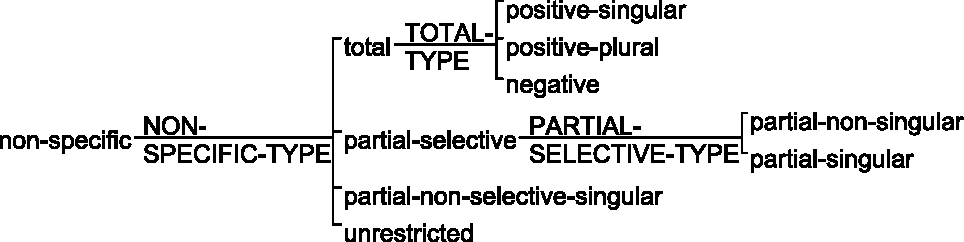
\includegraphics[width=0.9\linewidth]{Figures/SFL-grammar/determination-non-specific.pdf}
        \caption{The NON-SPECIFIC DETERMINATION system network}
        \label{fig:non-specific-deicticity}
    \end{figure}

    The dictionary lookup function outlined in Algorithm \ref{alg:dictionary-loockup} checks whether the word(s) of the CG node are in a dictionary. If the word is found then the function assigns the graph node with the associated features from the table. In addition, using the naive backwards induction method described in Algorithm \ref{alg:backward-induction-naive}, all the preselected features from a system network are determined and assigned to the graph node. %This works as a naive backwards induction of features from a delicate one up to the least delicate one at the root (see Algorithm \ref{alg:backward-induction-naive} in Section \ref{sec:system-networks-cs}). 
    An example of the dictionary is presented in the Table \ref{tab:lookup-dict-example} and the system network of NON-SPECIFIC determination is shown in Figure \ref{fig:non-specific-deicticity}.

\begin{table}[!ht]
    \centering
    \begin{tabular}{|l|l|}
        \hline
        \textit{Lexical item} & \textit{Feature}               \\ \hline
        a                     & partial-non-selective-singular \\ \hline
        all                   & positive-plural                \\ \hline
        either                & partial-singular               \\ \hline
        that                  & non-plural                     \\ \hline
    \end{tabular}
    \caption{Dictionary example for the NON-SPECIFIC DETERMINATION system network}
    \label{tab:lookup-dict-example}
\end{table}

    This section completed the explanation of how the MOOD features are assigned to the constituency graph. In the remainder of this chapter is addressed the task of assigning TRANSITIVITY process types and participant roles to the constituent units introduced in \citet{Costetchi2013}.

\section{Creation of empty elements}
\label{sec:creation-empty-elements}

    In the current work, when participants are missing but are syntactically recoverable in sentence then they are inferred from the structure and reference nodes are created for the missing elements. This phenomena is described in GB theory specifically as the \textit{Control and Binding} of empty elements \citep{Haegeman1991} introduced in Section \ref{sec:null-elements-gbt}. The \textit{reference constituents} are important for increasing the completeness and accuracy of semantic analysis by making the participants and their corresponding label explicit.

    This stage is particularly important for semantic role labelling because usually the missing elements are participant roles (theta roles) shaping the semantic configuration. The most frequent are the cases of \textit{control} where the understood subject of a clause is in the parent clause as in Examples \ref{ex:ctrl1}--\ref{ex:ctrl3} where \textit{Subj} is a generic subject placeholder introduced in Chapter \ref{ch:gbt} as \textit{PRO}, \textit{pro}, \textit{t-trace} and \textit{wh-trace}.

    \begin{exe}
    	\ex\label{ex:ctrl1}Poirot_i is considering whether [\textit{Subj_i} to abandon the investigation].
    	\ex\label{ex:ctrl2}Susan_i promised us [\textit{Subj_i} to help].
    	\ex\label{ex:ctrl3}They told you_i [\textit{Subj_i} to support the effort].
    \end{exe}

    There are also movement cases when a clause constituent receives no thematic role in a higher clause but one in a lower clause. The other case is of the non-overt constituents that are subjects in relative clauses and refer to the head of the nominal group. This part of the algorithm is set up to detect cases of \textit{null elements} as described in Section \ref{sec:placing-null-elements}, which relates GBT to Dependency Grammar and creates placeholder constituents for them which are in the next step enriched with semantic roles. Currently the NP traces and PRO subjects are created with a set of graph patterns, while the Wh traces are created with an algorithm.

\subsection{PRO and NP-trace Subjects}

    The \textit{xcomp} relation in DG can be encoded as a CG pattern graph (Figure \ref{fig:arb-control}) targeting the constituents that are non-finite clauses functioning as complement that have no subject constituent of their own and no ``if'' and ``for'' markers (according to generalisation \ref{gen:4}). They receive a PRO subject constituent (governed or not) by the parent clause subject.

    \begin{figure}[!ht]
    	\centering
    	\begin{tikzpicture}[tree-style,level distance=3em,level 1/.style={sibling distance=7em},] 
    	\node[pattern-node, anchor=center] (vb1){class:clause}
    	%child {node[pattern-node] (subj1) {class:nominal,\\element:subject,\\id:subj1}}
    	child {node[pattern-node,below = 2em of vb1,] (vb2) {element:complement,\\class:clause,\\finiteness:non-finite}
    		child {node[pattern-node-negative] (marker) {element:marker,\\words:[if,for]}}
    		child {node[pattern-node-negative] (subj2) {element:subject,\\operation:insert}}
    	};
    	\end{tikzpicture}
    	\caption{CG pattern for detecting PRO subjects}
    	\label{fig:arb-control}
    \end{figure}

    %%TODO either leave commented or rephrase
    %In terms SFG terms, if there is an Complement in the higher clause it is likely that it is the controller of the PRO in lower clause. Three role cognition verbs like in Example \ref{ex:pro7} take two complements where one of them is the phenomenon and can be a nominal group or a non-finite clause with PRO subject controlled by the object in higher clause.

    The generalisation \ref{gen:11} reflects criteria for selecting the controller of PRO based on its proximity in the higher clause. The schematic representation of the pattern for obligatory and subject object control (treated in Section \ref{sec:np-traces}) is depicted in Figures \ref{fig:obj-control} and \ref{fig:subj-control} respectively. In the case of Figure \ref{fig:subj-control} the prepositional complements do not affect subject control treatment in any way. The reason for that is because the graph pattern specifies only the nominal complements, which is complementary to object control pattern in Figure \ref{fig:obj-control}. %with respect to prepositional complements. 

    \begin{figure}[!ht]
    	\centering
    	\begin{tikzpicture}[tree-style,level distance=4em,level 1/.style={sibling distance=11em},] 
    	\node[pattern-node, anchor=center] (vb1){class:clause}
    	child {node[pattern-node] (subj1) {class:nominal,\\element:subject}}
    	child {node[pattern-node] (subj1) {class:nominal,\\element:complement,\\id:compl1}}
    	child {node[pattern-node] (vb2) {class:clause,\\element:complement,\\finiteness:non-finite}
    		child {node[pattern-node-negative] (marker) {element:marker,\\words:[if,for]}}
    		child {node[pattern-node-negative] (subj2) {element:subject,\\operation:insert,\\arg:\{id:compl1\}}}
    	};
    	\end{tikzpicture}
    	\caption{CG pattern for obligatory object control in complement clauses}
    	\label{fig:obj-control}
    \end{figure}
    
    \begin{figure}[!ht]
    	\centering
    	\begin{tikzpicture}[tree-style,level distance=4em,level 1/.style={sibling distance=11em},] 
    	\node[pattern-node, anchor=center] (vb1){class:clause}
    	child {node[pattern-node] (subj1) {class:nominal,\\element:subject,\\id:subj1}}
    	child {node[pattern-node-negative] (subj1) {class:nominal,\\element:complement}}
    	child {node[pattern-node] (vb2) {class:clause,\\element:complement,\\finiteness:non-finite}
    		child {node[pattern-node-negative] (marker) {element:marker,\\words:[if,for]}}
    		child {node[pattern-node-negative] (subj2) {element:subject,\\operation:insert,\\arg:\{id:subj1\}}}
    	};
    	\end{tikzpicture}
    	\caption{CG pattern for obligatory subject control in complement clauses}
    	\label{fig:subj-control}
    \end{figure}

    In dependency grammar the adjunct clauses are also introduced via \textit{xcomp} and \textit{prepc} relations, so syntactically there is no distinction between the two and patterns from Figures \ref{fig:obj-control} and \ref{fig:subj-control} are applicable.

    %%TODO introduce properly the discussion below about distinguishing the PRO and NP and about pre-marking the constituents with their potential to semantic roles

    %%todo this is discussed in sec:np-traces
    Before discussing each approach I would like to state that when the empty constituent is being created two important details are required: (a) the antecedent constituent it is bound to and (b) the type of relationship to its antecedent constituent or, if none is available, the type of empty element: t-trace or PRO. Now identifying the antecedent is quite easy and can be provided at the time of CG creation but since the empty element type may not always be available then it may have to be marked as partially defined.

    The first solution is to create the empty subject constituents based only on syntactic criteria, ignoring element type (either PRO or \textit{t}-trace) and hence postponing the decision to the semantic enrichment phase (addressed in this chapter). The advantage of doing this so is a clear separation of syntactic and semantic analysis. The empty subject constituents are created in the places where they should be and so this leaves aside the semantic concern of how the thematic roles are distributed. The disadvantage is leaving the created constituents incomplete or under-defined. Moreover the thematic role distribution must be done within the clause limits but because of raising, this process must be broadened to a larger scope beyond clause boundaries. This of course is an unwise approach as it might lead to unbounded dependencies and so unbounded complexity that needs to be addressed. 

    The second solution is to decide the element type before Transitivity analysis and remove the burden of complex patterns that go beyond clause borders. Also, all syntactic decisions would be made before semantic analysis and the empty constituents would be created fully defined with the binder and their type. But this means delegating semantically related decision to syntactic level (in a way peeking ahead in the process pipeline).

    In the current work, however, the semantic roles are addressed within the clause borders following the principle of one-main-verb-per-clause and thus avoiding the above mentioned risk of unbounded complexity. Also, the transitivity analysis is done based on pattern matching. This means a tremendous rise in complexity as the scope of a graph pattern is extended to two or more clauses. Instead, a desirable solution is iteration over all the clauses in the CG (a sentence) and matching semantic patterns within the clause boundaries one at a time.

    The solution adopted here is a mix of the two described above and addresses the issues of: (a) increasing the complexity of patterns for transitivity analysis, (b) leaving undecided which constituents accept thematic role in the clause and which do not. 

    The process to distinguish the empty constituent type starts by (a) identifying the antecedent and the empty element (through matching the subject control pattern in Figure \ref{fig:subj-control}), (b) identifying the main verbs of higher and lower clauses and correspondingly the set of possible configurations for each clause (by inquiry to the process type database (PTDB) described in the transitivity analysis Section \ref{sec:semantic-parsing}).

    If conditions from Generalisation \ref{gen:trace-detection} (from Section \ref{sec:np-traces}) are met then the empty constituent is a subject controlled \textit{t}-trace. Now we need a set of simple rules to mark which constituents receive a thematic role. These rules are  presented in Generalisation \ref{gen:thematic-marking} below.

    \begin{generalization}\label{gen:thematic-marking}
        Constituents receiving thematic roles are marked with a ``thematic-role'' label, those that do not receive a thematic role are marked with ``non-thematic-role'' and those that might receive thematic role with ``unknown-thematic-role''. So in each clause:
        \begin{itemize}
            \item the subject constituent is marked with thematic-role label unless (a) it is an expletive or (b) it is the antecedent of a \textit{t}-trace; then marked non-thematic-role
            \item a complement constituent that is an nominal group (NP) or an embedded complement clause is marked with thematic-role label.
            \item a  complement that is a prepositional group (PP) is marked with unknown-thematic-role.
            \item a complement that is a prepositional clause is marked with unknown-thematic-role label unless they are introduced via ``that'' and ``whether'' markers then it is marked with thematic-role label.
            \item the adjunct constituents are marked with non-thematic-role.
        \end{itemize}
    \end{generalization}

    According to Generalisation \ref{gen:9} PRO is optionally controlled in subject non-finite clauses. Since it is not possible to bind PRO solely on syntactic grounds Generalisation \ref{gen:9} proposed the arbitrary interpretation, i.e. no binding to an antecedent; and this is the solution adopted in this work for PRO elements.

    \begin{figure}[!ht]
    	\centering
    	\begin{tikzpicture}[tree-style,level distance=3em,level 1/.style={sibling distance=7em},] 
    	\node[pattern-node, anchor=center] (vb1){class:clause}
    	%	child {node[pattern-node] (subj1) {class:nominal,\\element:subject,\\id:subj1}}
    	%	child {node[pattern-node-negative] (subj1) {class:nominal,\\element:complement}}
    	child {node[pattern-node, below =2em of vb1, anchor=north] (vb2) {class:clause,\\element:subject,\\finiteness:non-finite}
    		child {node[pattern-node-negative, below =2em of vb2, anchor=north] (subj2) {element:subject,\\operation:insert,\\arg:\{words:one\}}}
    	};
    	\end{tikzpicture}
    	\caption{CG pattern for arbitrary control in subject clauses}
    	\label{fig:subj-arbitrary-control}
    \end{figure}

    The pattern for subject control in a subject clause  is represented in Figure \ref{fig:subj-arbitrary-control}. This of course is an oversimplification and more rigorous binding rules would need to be developed in future work to cover binding scenarios exemplified in Examples \ref{ex:pro12}--\ref{ex:pro15}.

\subsection{Wh-trances}
    Creating constituents for Wh-traces involved a slightly larger number of scenarios and for pragmatic reasons I implemented the following algorithm rather than create the set of corresponding graph patterns. Nevertheless in future work this should be expressed as graph patterns in order to be consistent with the general approach of the thesis. Algorithm \ref{alg:create-wh-trace} shows how it is currently done.

    \begin{algorithm}[!ht]
    	\Input { \cg}
    	\Begin{
            \If {more than one clause in \cg}
            {
           		\For {\Element \KwTo list of Wh-elements in \cg}
           			{
           				identify the Wh-groups containing the \Element\;
           				identify the syntactic function of the Wh-element within the group\;
           				identify the function of Wh-group in the clause\;
           				%check the number of clauses and which of clauses contains the Wh-group\;
        				\For(low to high){\Group \KwTo \cg}
        					{\If{Wh-group is \textbf{not} Subject \textbf{AND}\\ Wh-group is \textbf{not} in lowest embedded clause}
        						{
        						\eIf{Wh-group is Adjunct function}
        						{create Adjunct Wh-trace using \dg and \cg}
        						{create Theta Wh-trance using \dg and \cg}
        						}
        					}	
           			}
    		}
    	}
    	\caption{Creating the Wh-traces}
    	\label{alg:create-wh-trace}
    \end{algorithm}

    The first line of the algorithm checks if there are more than one clause in the CG, otherwise it cannot continue. Then all the Wh-elements, their functions within the group and the clause identified. Then, from the lower to higher, clauses are iterated and the constituent corresponding to Wh-trace in the lower clause is created and linked to the trace constituent in the parent clause. The creation of the Adjunct or Theta Wh-traces involves different procedures. The corresponding algorithms have been omitted in this section but are included in the Appendix \ref{ch:extra-pseudo-code}. 

    After the null elements are created the constituency graph is ready for the semantic enrichment stage, and semantic configurations are assigned to each clause. The next sections introduce first how the PTDB has been normalised and how the graph patterns are created from it; they then proceed with the semantic enrichment algorithm.

\section{Cleaning up the PTDB}
\label{sec:claning-ptdb}

    The original version of the PTDB available on Neale's personal page\footnote{see \url{http://www.itri.brighton.ac.uk/~Amy.Neale/}} is not usable for computational purposes as such. It  contains records applying a couple of different notations and sometimes informal comments for human understanding, which from a machine standpoint are noise and cannot be processed as such. In this section I explain how the original PTDB was transformed into a machine readable form in order to be used as a lexical database.

    The internal structure of the PTDB is detailed in Neale's PhD thesis \citep[193--231]{Neale2002}. Here I focus on three columns which are of interest for the parsing process: the \textit{verb form} ($1^{st}$), the Cardiff grammar \textit{process type} ($6^{th}$) and the participant role \textit{configuration} ($8^{th}$). Note that column numbers correspond to the original PTDB structure. After the transformation the PTDB column descriptions are as described in Table \ref{tab:ptdb-comparison}. The field names in italics are the ones of interest and have been modified.

    \begin{table}[!ht]
    	\centering
    	\begin{tabulary}{\textwidth}{|l|L|L|}
    		\hline
    		\textbf{Column} & \textbf{Original}                    & \textbf{Modified}                                         \\ \hline
    		1/A             & Form                                 & Form                                                      \\ \hline
    		2/B    & \textit{Occurences of form}          & \textit{Occurences of form}                               \\ \hline
    		3/C             & COB class (\& figure where possible) & COB class (\& figure where possible)                      \\ \hline
    		4/D             & meaning descrition                   & meaning descrition                                        \\ \hline
    		5/E             & Occurences in 5 million words        & Occurences in 5 million words                             \\ \hline
    		6/F    & \textit{Cardiff Grammar feature}     & \textit{Cardiff Grammar process type (reindexed/renamed)} \\ \hline
    		7/G             & Levin Feature                        & \textit{Cardiff participant feature}                      \\ \hline
    		8/H             & \textit{Participant Role Configuration}       & \textit{Cardiff participant feature (extra)}              \\ \hline
    		9/I             & Notes                                & Levin feature                                             \\ \hline
    		10/J            &                                      & \textit{Participant Role Configuration}                   \\ \hline
    		11/K            &                                      & Notes                                                     \\ \hline
    	\end{tabulary}
    	\caption{The table structure of PTDB before and after the transformation}
    	\label{tab:ptdb-comparison}
    \end{table}

    Next I describe the transformed PTDB and how it is interpreted. For a start, the verb form column contains either the base form of the verb (e.g. draw, take), base form plus a preposition (e.g. draw into, draw away, take apart, take away from) or the base form plus a phraseologic expression (e.g draw to an end, take on board, take the view that, take a shower). The prepositions are either the verbal particles or the preposition introducing the prepositional phrase complement. Prepositions often influence the process type and the participant configuration. So they are important cues to consider during semantic role assignment. The verb forms that have the same process type and configuration but different prepositions are often grouped together delimited by a slash ``/'' (e.g. draw into/around, take off/on) or if optional (i.e. coincide with the meaning of the verb base form without any preposition), they are placed in round brackets ``()'' (e.g. flow (into/out/down) ).

    The process type column registers one feature from the PROCESS-TYPE systemic network depicted in Figure \ref{fig:cardiff-transitivity}, which was introduced in Section \ref{sec:transitivity}. The participant configuration column contains a sequence of participant type abbreviations joined by a plus sign ``+'' (e.g. Ag + Af, Em + Ph, Ag-Cog + Ph). The order of participants corresponds to the Active voice in Declarative mood, also called the \textit{canonical form of a configuration} described in \citet{Fawcett2009}. Originally the configurations contained the ``Pro'' abbreviation signifying the place of the main verb/process. As all configurations are in canonical form, the Pro was redundant occurring always in the second position thus has been removed. So the first participant, in canonical form, corresponds to the Subject, the second to the first complement and the third to the second complement. Some participants are optional for the meaning and are marked with round brackets ``()'', e.g. Ag + Af-Ca (+ Des), meaning that the participant may or may not be realised. Sometimes, for directional or locational process types, the second or third participants may function as Adjuncts, which currently complicates the matching process.

    Not all the records in the original resource fulfil the description above and so needed corrections. For example when Neale had doubts during the making of PTDB, she marked uncertainties with a question mark ``?''. In addition, the ``,'' (comma) and ``\&'' (and) signs are used inconsistently with various meaning in all columns. Also, comments such as ``not in Cob'' (i.e. not in Cobuild presumably) were encountered in several columns.

    Some records contain only prepositions listed in the verb form column, which actually represents omissions of the main verb that is to be found in the immediately preceding records(s); this have been fixed by pre-pending the verb form to the preposition. 

    %The account of verb meanings in PTDB is not exhaustive. Compared to VerbNet or FrameNet there are considerably less meanings described. 

    Among the identified verb meanings in PTDB, there are also some that do not contain configurations. These records missing a process type and configuration have been suppressed. 

    The process type feature column contained originally a second feature which has been removed; it represented a compressed version of the participant configuration and it was redundant as the full configuration is registered in the next column. 

    In the PTDB Neale uses the slightly different process type names than the ones used in this work. The process type features have been thus re-indexed and adapted to match exactly the feature labels in the PROCESS-TYPE systemic network (e.g. ``one role action'' became ``one-role-action'', ``emotion plus xxx'' became ``emotive'', ``cognition xxx'' became ``two-role-cognition''). Appendix \ref{ch:reindexing-ptdb} provides the mapping across the process type versions. 

    The configuration column is one of the most important in the PTDB. Checking its consistency with respect to Fawcett's Transitivity system revealed the need for some corrections. For example ``Af + Af'', ``Af-Ca + Pos + Ag'', ``Af-Cog + Ph + Ag'' are grammatically impossible configurations and were manually corrected to the closest likely configuration ``Ag + Af'', ``Ag + Af-Ca + Pos'', ``Ag + Af-Cog + Ph''.

    Other records, judged by the process type, were incomplete. For example instances of two role actions registered only one of the roles, e.g. Af or Ca omitting the Ag participant. These records have also been manually corrected by prepending the Ag, Ag-Af or Cog roles depending as appropriate. 

    %\begin{figure}[!ht]
    %    \centering
    %    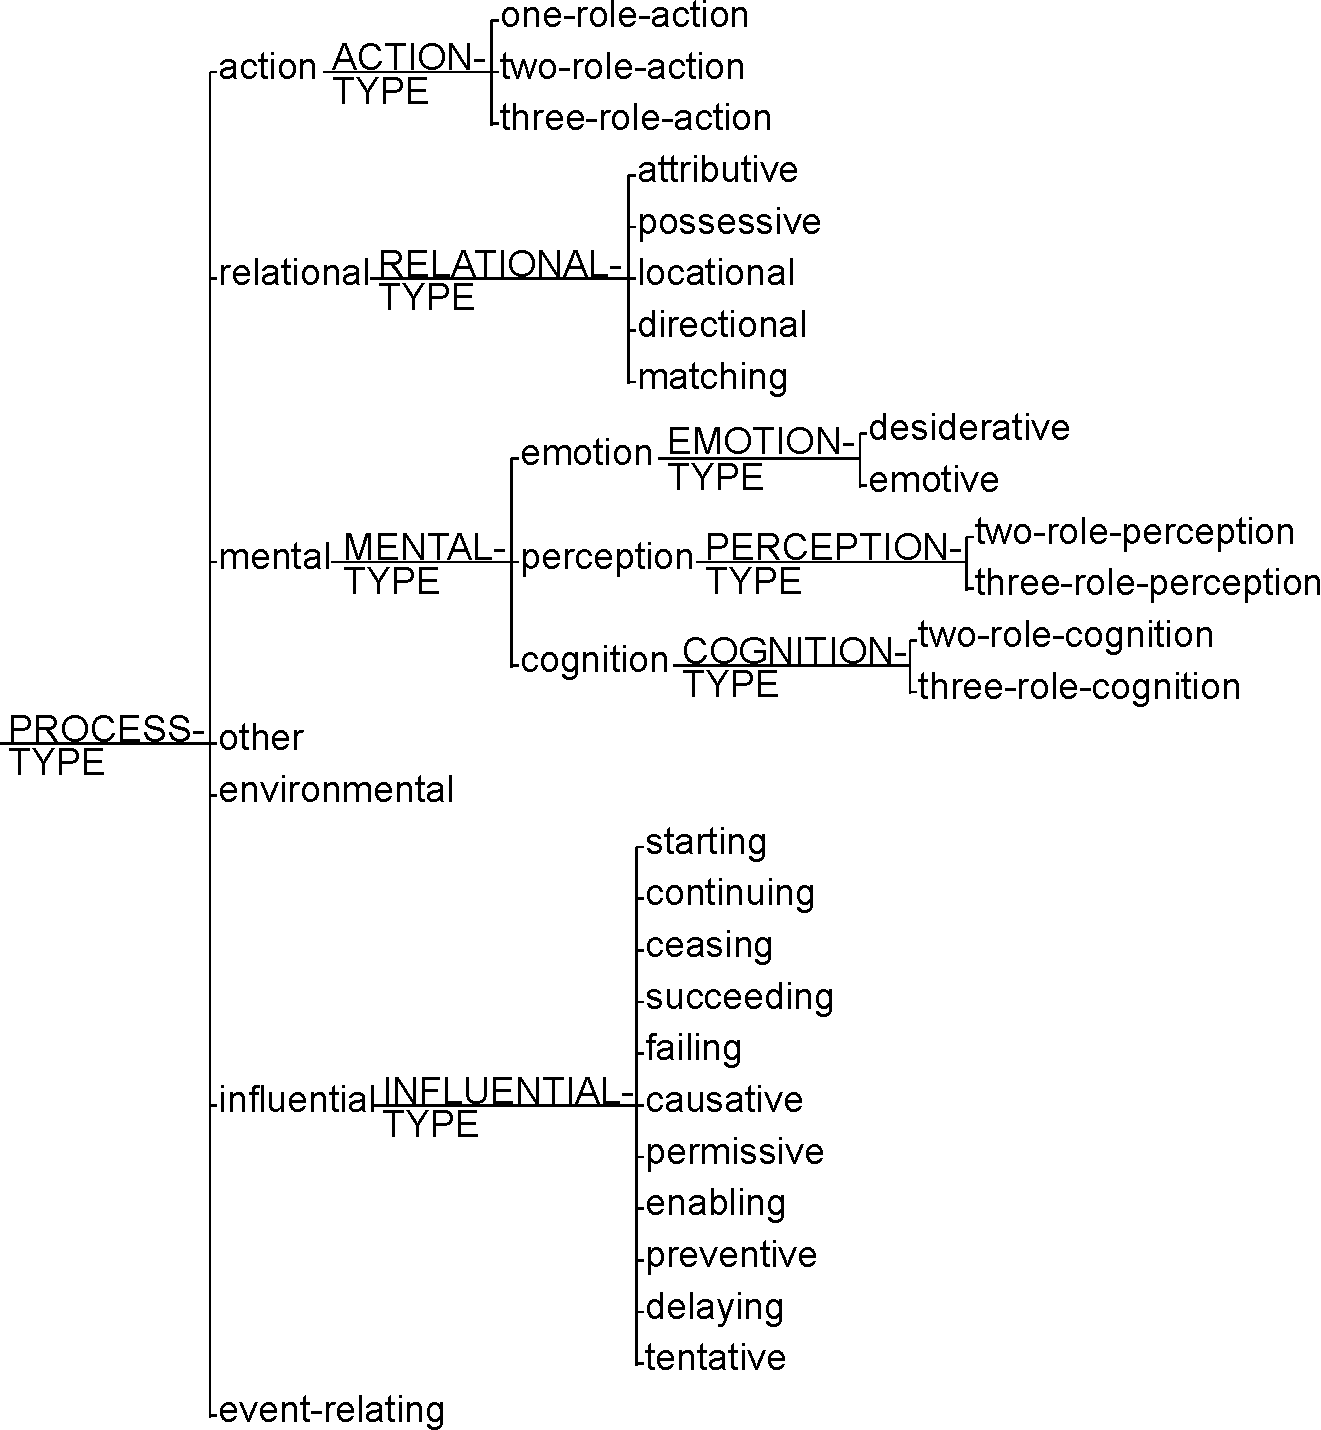
\includegraphics[width=0.7\linewidth]{Figures/SFL-grammar/Transitivity}
    %    \caption{TRANSITIVITY system network in Cardiff Grammar} %[TRANSITIVITY system network in Cardiff Grammar]
    %    \label{fig:transitivity-system}
    %\end{figure}

    The ``Dir'' participant is interpreted as direction but is not registered/defined in the Cardiff Grammar. Nevertheless there is a ``Des'' participant which I believe is the closest match. Therefore all ``Dir'' occurrences have been changed to ``Des''. One may argue that the two have different meanings however grammatically they seem to behave the same (at least in the accounted configurations). 

    By contrast some process types have been changed from action into either locational or directional because they contained either ``Loc'' (location), ``Des'' (destination) or ``So'' (source) participants which are not found in action processes unless they function as adjuncts, which are out of the context of the current description.

    A note worth making here is that locational, movement specifically but also other spatial verbs are very difficult to assign roles correctly because their participants are locations, directions, destinations etc., which can also serve as spatial adjuncts. This aspect has not been directly addressed in present work and is reflected in the evaluation results (that will be presented in Chapter \ref{ch:evaluation}) with a lower accuracy for these process types than others.

    The Cardiff features column indicates the process type selected in the TRANSITIVITY system corresponding to one of the top levels depicted in Figure \ref{fig:cardiff-transitivity} provided in Chapter \ref{ch:the-grammar}. Next section provides a description of how the graph patterns are generated from the PTDB. 

\section{Generation of the TRANSITIVITY graph patterns}
\label{sec:gen-sem}
    The configuration pattern graphs are used for CG enrichment executed through graph matching operation as described in Section \ref{sec:pattern-graph-matching}. In the previous section we saw how the PTDB has been cleaned up and normalised to support automatic generation of the \textit{Configuration Graph Patterns} (CGP), which afterwards are used to enrich constituency graphs with transitivity features. These graph patterns represent a constrained syntactic structure that carries semantic features that  are applied if the pattern is identified. 

    CGPs are generated from the process type and participant configuration columns of the PTDB. Figure \ref{fig:general-configuration-canonic} depicts the prototypical template for generating a three role CGP for canonical participant order that is active VOICE and declarative MOOD. This pattern matches declarative clause with a subject and two complements and in case of success updates the constituents with process type and participant roles. When the configuration has only one or two participants the graph pattern indicates one or two negative complement nodes as depicted in Figures \ref{fig:general-configuration-canonic-two} and \ref{fig:general-configuration-canonic-one-partic}. In this section I do not aim at providing an exhaustive account of all the pattern forms but explain the principles by which they are automatically generated.

    \begin{figure}[!ht]
    	\centering
    	\begin{tikzpicture}[tree-style, level distance=4em, level 1/.style={sibling distance=12em},] 
    	\node[pattern-node, anchor=center] (proc){class:clause,\\MOOD:declarative, VOICE:active\\operation:update,\\ arg1:\{process:process-type\}}
    	child{node[pattern-node]{element:subject,\\operation:update,\\ arg1:\{participant:role1\}} edge from parent node[left] {}}
    	child{node[pattern-node]{element:complement,\\operation:update,\\ arg1:\{participant:role2\}} edge from parent node[below] {}}
    	child{node[pattern-node]{element:complement,\\operation:update,\\ arg1:\{participant:role3\}} edge from parent node[right] {}};
    	\end{tikzpicture}
    	\caption{Declarative MOOD and active VOICE graph pattern with three participant roles}
    	\label{fig:general-configuration-canonic}
    \end{figure}
    
    \begin{figure}[!ht]
    	\centering
    	\begin{tikzpicture}[tree-style, level distance=4em, level 1/.style={sibling distance=12em},] 
    	\node[pattern-node, anchor=center] (proc){class:clause,\\MOOD:declarative, VOICE:active\\operation:update,\\ arg1:\{process:process-type\}}
    	child{node[pattern-node]{element:subject,\\operation:update,\\ arg1:\{participant:role1\}} edge from parent node[left] {}}
    	child{node[pattern-node]{element:complement,\\operation:update,\\ arg1:\{participant:role2\}} edge from parent node[below] {}}
    	child{node[pattern-node-negative]{element:complement} edge from parent node[below] {}};
    	\end{tikzpicture}
    	\caption{Declarative MOOD and active VOICE graph pattern with two participant roles}
    	\label{fig:general-configuration-canonic-two}
    \end{figure}
    
    \begin{figure}[!ht]
        \centering
        \begin{tikzpicture}[tree-style, level distance=4em, level 1/.style={sibling distance=12em},] 
        \node[pattern-node, anchor=center] (proc){class:clause,\\MOOD:declarative, VOICE:active\\operation:update,\\ arg1:\{process:process-type\}}
        child{node[pattern-node]{element:subject,\\operation:update,\\ arg1:\{participant:role1\}} edge from parent node[left] {}}
        child{node[pattern-node-negative]{element:complement} edge from parent node[below] {}}
        child{node[pattern-node-negative]{element:complement} edge from parent node[right] {}};
        \end{tikzpicture}
        \caption{Declarative MOOD and active VOICE graph pattern with one participant role}
        \label{fig:general-configuration-canonic-one-partic}
    \end{figure}

    Besides the canonical CGP a set of variations are generated for each configuration corresponding to yes-no and Wh-Subj/Wh-obj/Wh-adj interrogative forms, imperative form and to passive voice form. 
    %The variations are function of the process type, participant roles, mood and voice. 
    When each of the variants are supported by the process type and participant configuration, the following CGP are generated: (1) the declarative active (2) the passive (3) the imperative and (4) Wh-interrogative (Wh-Subj/Wh-obj/Wh-adj especially important for locational and directions processes).

    %\explain{how do the process type influence the generated forms and also how the participant roles influence the forms?}
    %\explain{How do the CGP vary according to other features such as voice and mood}
    %\explain{What happens in Wh-Subj/Wh-obj/Wh-adj? what happens in Wh-YN, how are the patterns generated to cove those?}
    
    If the configuration accepts passive voice, i.e. the first participant in the configuration is not the expletive ``there'' or the pleonastic ``it'' and the last role is not Agent role, then both active and passive voice CPG are generated. Otherwise the passive form is not possible. 

    The imperative form CGP is generated if the first role of the configuration implies an active animate entity. Thus the nominal features of the subject must already be provided. Roles that accept imperative form are: Agent, Emoter, Cognizant, Perceiver and their compositional derivations, e.g. Agent-Carrier, Agent-Cognizant, Affected-Emoter etc. Clausal subjects are excluded. 

    The passive differs from the active voice pattern by switching the places of the first two roles resulting in the second role matched to the subject function and the first role to the first complement. In the case of imperative, the first role  as well as the subject constituent are simply omitted.  

    Algorithm \ref{alg:generating-cpg} outlines how the CPGs are generated from the PTDB. The CPGs are represented as Python structures and are stored in a Python module. This way the graph patterns are accessible as native structures making it easy to instantiate and execute the graph patterns. The process types are also grouped by the process type and number of participants which reduces the number of patterns be match per clause.  

    \begin{algorithm}[!ht]
    	\Input { PTDB }
    	\Begin{
    		generate unique set of process type + participant roles\;
    		generate unique set of process types\;
    		\For{process type \KwTo possible process type}
    		{
    			%generate configuration set for given process type \;
    			\For{configuration \KwTo configuration set}
    			{
    				generate declarative active pattern graph \;
    				\If {no expletive in configuration}
    				{
    					\If{configuration accepts passive}
    					{
    						generate declarative passive pattern graph\;
    					}
    					\If{configuration accepts imperative}
    					{
    						generate imperative pattern graph\;
    					}
    					\If{locational process}
    					{
    					generate expletive there pattern graph \;
    					}
    					\If{configuration participants may function as Adjuncts}
    					{
    						\tcc{the Directional processes varying optional Source, Path and Destination}
    						generate variate role indicative active pattern graphs \;
    						generate variate role indicative passive pattern graphs \;
    						generate variate role imperative pattern graphs \;
    						generate variate role Wh-interrogative pattern graphs \;
    					}
    				}
    			}
    		}
    	}
    	\caption{Generating the CPGs from the PTDB}
    	\label{alg:generating-cpg}
    \end{algorithm}

    The first two lines of the algorithm synthesise the PTDB by grouping unique configurations for each process type. Then for each configuration of each process type one to three pattern graphs depending on the configuration and process type specifics are generated.

    \begin{figure}[!ht]
    	\centering
    	\begin{tikzpicture}[tree-style, level distance=4em, level 1/.style={sibling distance=12em},] 
    	\node[pattern-node, anchor=center] (proc){class:clause,\\MOOD:declarative, VOICE:passive\\operation:update,\\ arg1:\{process:process-type\}}
    	child{node[pattern-node]{element:subject,\\operation:update,\\ arg1:\{participant:Role2\}} edge from parent node[left] {}}
    	child{node[pattern-node]{element:complement,\\operation:update,\\ arg1:\{participant:Role1\}} edge from parent node[below] {}}
    	child{node[pattern-node]{element:complement,\\operation:update,\\ arg1:\{participant:Role3\}} edge from parent node[right] {}};
    	\end{tikzpicture}
    	\caption{Declarative MOOD and passive VOICE graph pattern with three participant roles}
    	\label{fig:general-configuration-passive}
    \end{figure}
    
    \begin{figure}[!ht]
    	\centering
    	\begin{tikzpicture}[tree-style, level distance=4em, level 1/.style={sibling distance=12em},]
    	\node[pattern-node, anchor=center] (proc){class:clause,\\MOOD:imperative, operation:update,\\ arg1:\{process:process-type\}}
    	child{node[pattern-node-negative]{element:subject} edge from parent node[left] {}}
    	child{node[pattern-node]{element:complement,\\operation:update,\\ arg1:\{participant:Role2\}} edge from parent node[below] {}}
    	child{node[pattern-node]{element:complement,\\operation:update,\\ arg1:\{participant:Role3\}} edge from parent node[right] {}};
    	\end{tikzpicture}
    	\caption{Imperative MOOD graph pattern with three participant roles}
    	\label{fig:general-configuration-imperative}
    \end{figure}

    %\todo{Explain the rules by which are created variations on voice, mood (and other features) based on configuration type and participants}
    The declarative MOOD active VOICE pattern (depicted in Figure \ref{fig:general-configuration-canonic}) corresponding to the canonical form in PTDB is always generated. If the configuration does not contain an expletive and accepts passive voice then the corresponding pattern is generated with the first and second roles switched as in Figure \ref{fig:general-configuration-passive}. Note that role2 is assigned to the subject and role1 to the first complement. If the configuration accepts imperatives, then also a subject-less pattern graph is generated with the first role omitted as depicted in Figure \ref{fig:general-configuration-imperative}. 

    Directional processes are a special case. Examples \ref{ex:directional2} to \ref{ex:directional4} are equally valid configurations. Example \ref{ex:directional5} is a generic representation highlighting the optionality of these participants. 
    %\todo{Discuss Neale/Fawcett possible configurations}
    \begin{exe}
    	\ex\label{ex:directional2} The parcel travelled from London[So].
    	\ex\label{ex:directional3} The parcel travelled via Poland[Pa].
    	\ex\label{ex:directional4} The parcel travelled to Moscow[Des].
    	\ex\label{ex:directional5} The parcel travelled (from London[So]) (via Poland[Pa]) (to Moscow[Des]).
    \end{exe}

    And so in directional configurations, second, third and fourth participants are optional and may occur in any order, but at least one of them should be present. Therefore So, Pa and Des participants patterns should be generated for all combinations as presented in Table \ref{tab:directional-partic-variations}.

    \begin{table}[!ht]
    	\centering
    	\begin{tabular}{|c|c|c|}
    		\hline
    		\textbf{So} & \textbf{Pa} & \textbf{Des} \\ \hline
    		\textbf{+} & - & - \\ \hline
    		- & \textbf{+} & - \\ \hline
    		- & - & \textbf{+} \\ \hline
    		\textbf{+} & \textbf{+} & - \\ \hline
    		\textbf{+} & - & \textbf{+} \\ \hline
    		- & \textbf{+} & \textbf{+} \\ \hline
    		\textbf{+} & \textbf{+} & \textbf{+} \\ \hline
    	\end{tabular}
    	\caption{Participant arrangements for Directional processes (order independent)}
    	\label{tab:directional-partic-variations}
    \end{table}

    Finally, the CPGs are grouped by process type. This alleviates the burden of selecting the number of patterns to test for a certain clause. 

    %The python structure looks as represented in Listing \ref{lst:config-pattern-set}
    %\begin{lstlisting}[language=json,firstnumber=1, caption={Configuration Pattern Set as a Python dictionary structure},label={lst:config-pattern-set}]
    %configuration_pattern_set = {
    %	process_type1 : {
    %		config1 : [pattern1, panttern2,...],
    %		config2 : [pattern3, panttern4,...],
    %	},
    %	process_type2 : {
    %		config3 : [pattern5, panttern6,...],
    %		config4 : [pattern7, panttern8,...],
    %	}
    %	...
    %}
    %\end{lstlisting}

    The patterns are generated in advance and so at runtime are ready for execution. This decreases execution time. Next follows the description of how the generated configuration graph patterns are used in the Transitivity enrichment phase.

\section{Enrichment with TRANSITIVITY features}
\label{sec:semantic-parsing}

    Once the constituency graph has been enriched with MOOD and nominal DEIXIS features and the null elements created, it is ready to be enriched with TRANSITIVITY features. The algorithm identifies, in each clause, the main verb and the potential participant constituents and searches in the PTDB for the lexical item matching the main verb and any of its extensions filtering (based on the clause constituency) the possible configurations for the verb (comprising all the verb configurations). Then all the graph patterns corresponding to the possible configurations are executed on the clause, which, if matched, will enrich the clause CG. 

    \begin{algorithm}[!ht]
        \Input { \cg, \dg }
        \Begin
        {
            \For{ clause \KwTo clauses in mcg}
            {
                select from PTDB candidate process types and configurations\;
                filter configurations fitting the clause \;
                \For{config \KwTo valid possible configurations}
                {
                    filter pre-generated pattern graphs of the config fitting the clause\;
                    \For{pattern \KwTo filtered pattern graph set}
                    {
                        \label{line:enrich-from-pattern} enrich clause using pattern and mcg filtered by role constraints\;
                    }
                }
            }
        }
        \caption{Transitivity parsing}
        \label{alg:transitivity-parsing}
    \end{algorithm}

    Algorithm \ref{alg:transitivity-parsing} outlines the semantic parsing process implemented in the current parser which is a cascade of three loops. The first loop iterates through clauses in the mood constituency graph and for each the candidate process types are identified by considering: (a) the main verb, (b) the prepositions connected to it (either prepositional particles, or prepositions introducing a complement or adjunct prepositional phrase listed in Table \ref{tab:participant-roles-constraints}) or (c) phrasal expressions such as ``take a shower'' which were explained in Section \ref{sec:ptdb-description-technical}.

    \begin{table}[!ht]
    	\centering
    	\begin{tabular}{|l|l|}
    		\hline
    		\textbf{Role} & \textbf{Prepositions}             \\ \hline
    		Des           & to,towards,at,on,in,              \\ \hline
    		Ben           & to,for,                           \\ \hline
    		Attr          & as,                               \\ \hline
    		Ra            & on,in,                            \\ \hline
    		So            & from,                             \\ \hline
    		Pa            & through,via,                      \\ \hline
    		Loc           & in,at,into,behind,in front of, on \\ \hline
    		Mtch          & with,to,                          \\ \hline
    		Ag            & by,                               \\ \hline
    		Ph            & about,                            \\ \hline
    		Cog           & to                                \\ \hline
    	\end{tabular}
    	\caption{Prepositional constraints on participant roles }
    	\label{tab:participant-roles-constraints}
    \end{table}

    The second loop iterates through the candidate configurations for each candidate process type and selects the graph patterns that should be matched to the current clause. Then iteratively, each of the retrieved graph patterns (in the third loop) are applied to the clause graph. Line \ref{line:enrich-from-pattern} enriches CG nodes with new features of the pattern graph each time they are successfully matched. Before enrichment the CG nodes are checked against an additional set of conditions (captured by Algorithm \ref{alg:role-constraint-check}) which were omitted in the pattern graph. These conditions may prevent enrichment even if the pattern has been identified. 

    %\explain{What is the selection/filtering based on ? probably subj/role, preposition/role constraints} The last set of checks is an attempt to reduce the false positive assignments. 
    %%For example if the complement is a clause then it can take only Phenomena role otherwise the entire

    \begin{algorithm}[!ht]
    	\Input {\node, role, \dg }
    	\Begin
    	{
    		\tcc{Cog, Em and Perc must be animates}
    		\If{role is Cog \textbf{or} Em \textbf{or} Perc}
    		{
    			check that the \node has animate feature \;
    		}
    		\tcc{clauses can only be phenomenas}
    		\If{\node is a clause}{
    			check that role is Ph only \;
    		}
    		\tcc{prepositional phrases can only start with certain prepositions for a role}
    		\If{\node is a Prepositional Phrase}
    		{
    			get the list of allowed prepositions for the role \;
    			check if the prepositional phrase starts with any of the allowed prepositions \;
    		}
    	}
    	\caption{Participant Role constraint check if a role is not illegal for constituent}
    	\label{alg:role-constraint-check}
    \end{algorithm}

    % The Transitivity parsing results in multiple process configurations being assigned to clauses decreasing, in a way, precision and or introducing uncertainty. Because the final result contains few possibilities without knowing which one is the case. This uncertainty, decreased with several heuristics, is not dealt with by the current parser and shall be addressed in the future work. 

\section{Summary}
%todo larger section

    This chapter has described how the constituency backbone is enriched with syntactic and semantic features from the MOOD and TRANSITIVITY system networks using graph patterns. Besides the core sections describing the enrichment algorithms, this chapter provides explanations about the graph pattern creation, CG extension with null elements and the clean-up of PTDB

    First null elements are identified and filled with proxy constituents. This process ensures higher accuracy of semantic role assignments from the configuration patterns in the second step. 

    The configuration patterns have been generated from the PTDB - a verb database accounting for Transitivity patterns in Cardiff grammar. In order to generate these patterns the PTDB had first to be cleaned up, unified and aligned to the present Transitivity system. Then for each configuration a set of possible patterns were generated, which vary based on mood, voice, process type and participants. Finally the semantic role labelling step employs the same pattern based enrichment mechanism as used in Section \ref{sec:enrichment-stage}.

    The algorithms can be improved by externalisation of constraints and conditions. In the next iterations of Parsimonious Vole parser development should be towards higher abstraction and separation between the grammatical constraints (in SFL represented as systemic realisation rules) and the algorithm.

\chapter{Empirical evaluation}
% \label{ch:evaluation}

% Chapter Introduction
% - set up the scene
% - state what is the aim of the evaluation (accuracy of the parser to segment text, 
% assign unit classes, element functions and systemic features to text segments)
% - explain how that aim is achieved (compare the segmentation, element assignment, 
% feature assignment available in the corpus with that coming from the parser)
% - how the chapter is structured  
% Main sections
% - describe the corpora
%   (provenance, annotations, size metrics, quality assessment; data examples ?)
% - describe the method of comparing parser output to corpus annotations 
% - present the evaluation data for: Mood and Transitivity elements + unit classes 
%   (focus on constituent identification)
% - present the evaluation data for: Mood and Transitivity features 
%   (focus on feature accuracy per system for the identified units)
% - *interpret evaluation data and present findings
%   (or should this be provided when each evaluation data is presented) 
% Conclusions
% - concise summary of the main findings


    This chapter aims to evaluate the Parsimonious Vole parser accuracy at generating text analysis in general; and how well it performs at unit boundary detection (i.e text segmentation), unit class assignment, element assignment and feature selections in particular. The grammar that is employed in this evaluation was introduced in Chapter \ref{ch:the-grammar} and the corpus will be introduced in Section \ref{sec:corpus}. 
    
    The evaluation data are collected by comparing the labelled segments  available in the corpus to the labelled segments in the parser output. The main measurements of parser accuracy considered here are \textit{precision} and \textit{recall} and $F_1$ scores. The parser \textit{precision} measures how many segments have been produced by the parser that are also found in manual analysis; and the parser \textit{recall} measures how many correct segments have been produced by the parser relative to the total number of produced segments. $F_1$ score is a harmonic mean of the precision and recall.
    
    The corpus used in this evaluation do not constitute a true gold standard and there are, due to different reasons, some differences to the parser. These differences will be described in detail in Section \ref{sec:differences}.
    
\noindent
\begin{minipage}{\linewidth}
\begin{lstlisting}[numbers=left,basicstyle=\small\tt, stepnumber=1,firstnumber=0,frame=single,caption=Example segment from the corpus,label=lst:exampleText1,escapeinside={(*}{*)}]
(*\textcolor{black!50}{$_{587}$}*)forced me into treatment(*\textcolor{black!50}{$_{611}$}*)
\end{lstlisting}
\end{minipage}

\noindent
\begin{minipage}{\linewidth}
\begin{lstlisting}[numbers=left,basicstyle=\small\tt, stepnumber=1,firstnumber=0,frame=single,caption=Example segment from the parser output,label=lst:exampleText2,escapeinside={(*}{*)}]
(*\textcolor{black!50}{$_{583}$}*)and forced me into treatment .(*\textcolor{black!50}{$_{612}$}*)
\end{lstlisting}
\end{minipage}    

The evaluation methodology, which will be described in detail in Section \ref{sec:evaluation-methodology}, considers perfect alignment between segment boundaries and their labels. Also it considers partial alignment of segments with the same label provided that the distance between them is not too large and there is not other better matching candidate at a shorter distance. This means that segment spans such as the ones in Listings \ref{lst:exampleText1} and \ref{lst:exampleText1} are given some credit in the alignment process. In this example, the segments are considered as partially (or closely) matching clauses. The main reason for taking segmentation discrepancies into consideration is for providing a wider evaluation ground to the systemic selections from the MOOD and TRANSITIVITY system networks. The next section describes the corpora used in current evaluation. 

\section{Evaluation corpus}
\label{sec:corpus}
    % (provenance, annotations, size metrics, quality assessment; data examples ?)
    
    This section briefly introduces the corpora used in the evaluation of the Parsimonious Vole parser. Table \ref{tab:corpus-sumary} provides a summary of the corpora descriptions.  
    
    \begin{table}[!ht]
        \centering
        \resizebox{\textwidth}{!}{%
        \begin{tabulary}{\textwidth}{cccccc}
            \toprule
            Corpus name & Meta-function & Characters & Clauses & Annotator(s) \\
            \midrule
            OCD & Mood & 16.200 & 147 &  Ela Oren \& Eugeniu Costetchi \\ 
            OE & Transitivity & 51.800 & 1503 & Anke Schultz \& Tatsiana Markovic \\ 
            OE-RRH & Transitivity & 5.600 & 157 & Anke Schultz \\
        \bottomrule
        \end{tabulary}
        }
        \caption{Evaluation corpus summary}
        \label{tab:corpus-sumary}
    \end{table}
    
    % TODO: introduce corpora
    
    
    % The OE corpus was not developed for the purpose of evaluating constituency in the current parser. Nevertheless the provided segmentation however can be used to evaluate the boundaries of constituent segments. This corpus are primitively used for evaluation of the constituent's semantic function and some TRANSITIVITY features (to the degree provided in the corpus). To enable each of these evaluations the annotation data and parser output needed to be uniformly represented in order to be in alignment with the parser output. To achieve this, feature names were harmonised with the ones from PTDB following the same adjustments as described in Section \ref{sec:claning-ptdb}. In Section \ref{sec:results},  the empirical findings of the current evaluation are described.

\subsection{OE corpus}

    The Bremen Translation Corpus (BTC) was created at the University of Bremen by Kerstin Fischer, Anatol Stefanowitsch and Anke Schulz. It consists of comparable and parallel texts. The comparable part consists of a series of newsgroup texts of about 10,000 words of English text and another 10,000 words of German, text taken from the same register. The parallel part, called EDNA, is much larger comprising about 100,000 words of parallel English-German text. Anke uses in her thesis 10,000 words of parallel text and about the same of comparable text \citep[31]{schulz2015me}. In this evaluation only the English part is considered which is called OE. It comprises 31 files spanning over 1503 clauses and 20864 words. In addition, Anke provided a set of similar annotations for the ``Little Red Riding Hood'' fairy tale, called OE-RRH, comprising 157 clauses that is included as part of OE corpus in this evaluation. 
    
    \begin{figure}[!h]
        \centering
        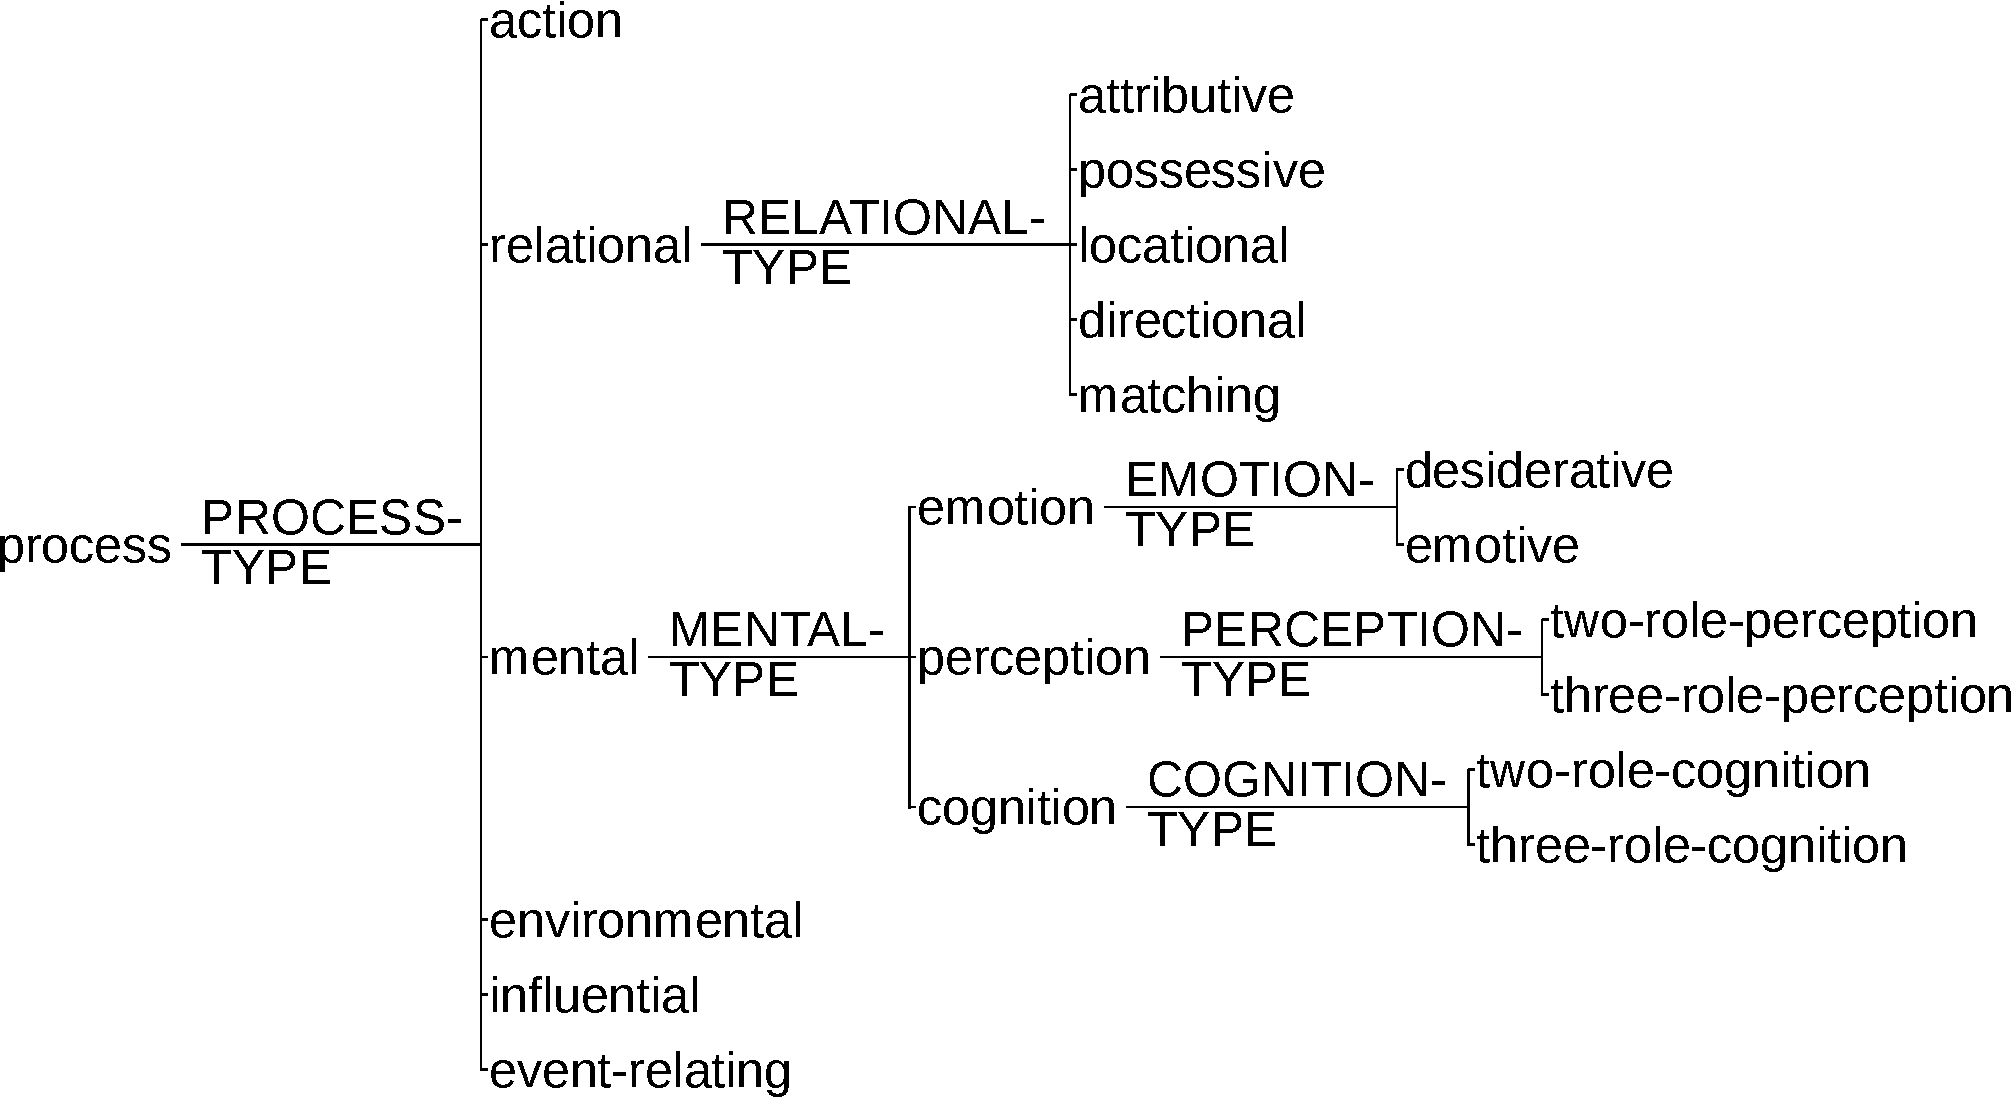
\includegraphics[width=.75\textwidth]{Figures/Evaluation/trans-simplified.pdf}
        \caption{The fragment of the TRANSITIVITY system network that has been used in the corpus}
        \label{fig:transitivity-simplified}
    \end{figure}

    The corpus annotations, developed by Anke Schulz and Tatsiana Markovic \citep[36]{schulz2015me}, cover Cardiff TRANSITIVITY, THEME and MODIFICATION system networks. The grammatical details and the annotation methodology are covered in detail in \citet[48-161]{schulz2015me}.
    
    For the purpose of the current evaluation only the TRANSITIVITY system was considered. The extent to which the system network is covered in the corpus annotations is limited to the top part of the original TRANSITIVITY system network. The used system network fragment is depicted in Figure \ref{fig:cardiff-transitivity}, while the whole system network was provided in the Chapter \ref{ch:the-grammar}. Employing the entire system network in the annotation process increases in difficulty as the delicacy increases due to the time needed to perform the task \citep[33]{mcenery2006corpus}. The challenge of providing delicate (or fine-grained) corpus annotations using the entire extent of a system network still has to be addressed in the SFL community. 
    

\subsection{OCD corpus}

     The first corpus (OCD) was created by Ela Oren and myself and is focused on syntactic constituency structure and clause MOOD features. The texts represent blog articles of people diagnosed with Obsessive Compulsive Disorder (OCD) who self-report on the challenge of overcoming OCD. The corpus contains four texts comprising all together 988 clauses and 8605 words. 

    \begin{figure}[!h]
        \centering
        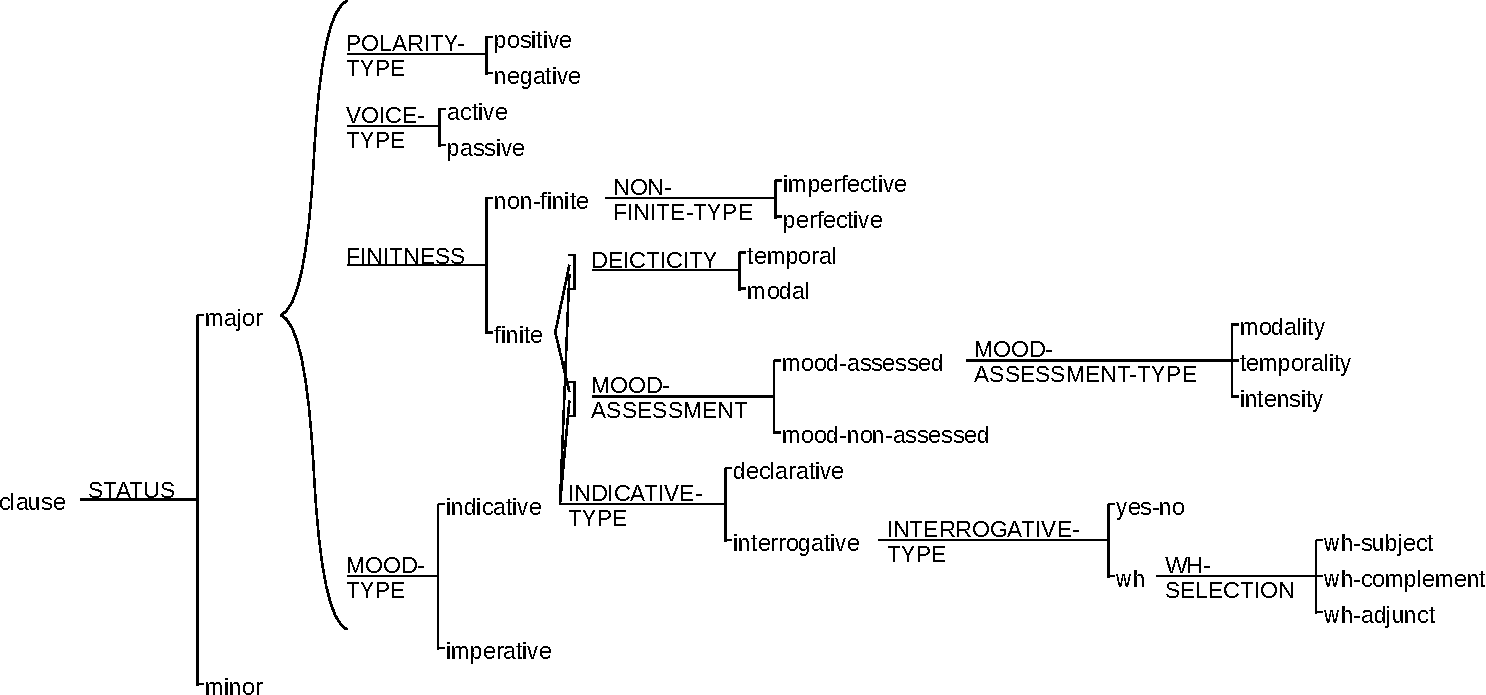
\includegraphics[width=.85\textwidth]{Figures/Evaluation/ocd1-mood-simplified.pdf}
        \caption{The part of the MOOD system network that has been used in OCD corpus annotation}
        \label{fig:mood-ocd-simplified}
    \end{figure}
    
    % todo expand, explain
    The corpus contains selections from the system network depicted in Figure \ref{fig:mood-ocd-simplified}. It is a sub-part of the MOOD system network supported by the Parsimonious Vole parser, which was described in Chapter \ref{ch:the-grammar} and depicted in Figure \ref{fig:clause-mood}. Employing the entire system network in the annotations was difficult because as the delicacy increases the time spent for the annotation process increases drastically making the annotation process very tedious and slow.
    


\subsection{Differences between the corpus annotation and parser output}
\label{sec:differences}

    This section describes the main known differences between how the parser structures output and the methodology used to annotate the corpus. These differences are mainly due to text normalisation, treatment of conjunctions and punctuation. In OCD corpus there are also some segmentation errors described below.
    
    The Parsimonious Vole parser after receiving the raw text, first operation it performs is that of text normalisation. In this process the tabs and extra spaces between words and are reduced and special characters such as quotes, parenthesis, dashes and other orthographic characters are re-represented in a uniform way. In the OE corpus most of the text is uniformly formatted but there are few deviations. 
    

\begin{minipage}{\linewidth}
\begin{lstlisting}[numbers=left,basicstyle=\small\tt, stepnumber=1,firstnumber=0,frame=single,caption=Sample of non-normalised raw text from the corpus,label=lst:exampleText,escapeinside={(*}{*)}]
(*\textcolor{black!50}{$_{0}$}*)Red riding hood excerpt(*\textcolor{black!50}{$_{24}$}*)
(*\textcolor{black!50}{$_{25}$}*)"What have you in that basket,   Little Red Riding Hood?"(*\textcolor{black!50}{$_{82}$}*)
(*\textcolor{black!50}{$_{83}$}*)
(*\textcolor{black!50}{$_{84}$}*)"Eggs and butter and cake, Mr. Wolf."(*\textcolor{black!50}{$_{111}$}*)
\end{lstlisting}
\end{minipage}

    Listing \ref{lst:exampleText} presents an example raw text from the annotation dataset containing an initial title line and two sentences separated by an empty line. The greyed index numbers at the beginning and end of each line indicate character offsets. In OE corpus files, the first line plays the role of a header containing the title or the file name. In this example it is a title. Either way, this first line is neither considered for annotation nor parsing. 
    
    In the OCD corpus normalisation was not at all addressed before the annotation started. Mostly it is organised as one sentence per line, but there are instances of extra blank lines or missing new line characters leading to few sentences per line as a block. The text may also contain tabs and extra blank spaces or blank lines as in Listing \ref{lst:exampleText} at index [82,84]. 

    It is noteworthy to mention that there are segmentation errors in a few cases from the OCD corpus. Some segments are either shifted and include the adjacent spaces (e.g. `` getting this push'' instead of ``getting this push'') or, the converse, leave out one or two characters of a marginal word (e.g. ``the balanc'' instead of ``the balance''). Such 

    As mentioned in the beginning of this section, the parser diverges in a few ways from the corpus annotation methodology when it comes to punctuation marks and treatment of conjunctions. Unfortunately there was no time to create a true golden corpus but OCD and OE corpora are close to that. 

    In the OCD and OE corpus annotations, punctuation marks such as commas, semicolons, three dots and full stops are not included in the constituent segments while the parser includes them at the end of each adjacent segment. 
    
    \begin{figure}[!ht]
        \centering
        \begin{subfigure}[b]{0.47\textwidth}
            \centering
            \begin{tikzpicture}[pattern-node]
            \node[pattern-node] (start) {};
            \node[pattern-node, right = 5em of start] (end) {};
            \draw[edge-style] (start) -- (end) node[midway, above]{conjunct 1};
            
            \node[pattern-node, right = .5em of end] (conj) {and};
            
            \node[pattern-node, right = .5em of conj] (start1) {};
            \node[pattern-node, right = 5em of start1] (end1) {};
            \draw[edge-style] (start1) -- (end1) node[midway, above]{conjunct 2};
            
            \end{tikzpicture}
            \caption{Conjuncts annotated as parallel segments}
            \label{fig:segment-conjunction-paralel}
        \end{subfigure}
        \quad
        \begin{subfigure}[b]{0.47\textwidth}
            \centering
            \begin{tikzpicture}[pattern-node] 
            \node[pattern-node] (start) {};
            \node[pattern-node, right =14em of start] (end) {};
            \draw[edge-style] (start) -- (end) node[midway, above]{conjunct 1};
            
            
            \node[pattern-node, below = 0.1em of end] (end1) {};
            \node[pattern-node, left = 8em of end1] (start1) {};
            \draw[edge-style] (start1) -- (end1) node[midway, above]{conjunct 2};
            
            \node[pattern-node, below = -0.6em of start1, xshift=1.8em] (conj) {and};        
            \end{tikzpicture}
            \caption{Conjuncts annotated as subsumed segments}
            \label{fig:segment-conjunction-subsumed}
        \end{subfigure}
        \caption{Treatment of conjunctions in the corpus compared to the parser}
        \label{fig:conjunction-treatment}
    \end{figure}
    
    The treatment of conjunctions that was discussed in Section \ref{sec:coordination} differs as well. In the corpus, the conjunctions (such as ``and'', ``but'', ``so'', etc.) are excluded from the conjunct segments; they are considered markers in the clause/group complexes rather than part of the constituent. The parser, on the other hand, includes the conjunctions in the following adjacent segment. For example in the corpus there we find segment ``forced me into treatment'' while the parser produces a slightly larger segment ``and forced me into treatment.'' that includes the conjunction at the beginning and the full-stop at the end.
    
    Moreover the conjunct segment spans differ as well due to difference in treatment. Instead of being analysed in parallel, having sibling status as depicted in Figure \ref{fig:segment-conjunction-paralel}, the parse generated conjunct segments are subsumed in a cascade from the former to the latter as depicted in Figure \ref{fig:segment-conjunction-subsumed}.
    
    In this section were mentioned the most important aspects in which the corpora annotations and parser output diverge. The evaluation methodology has been developed to take segmentation discrepancies into consideration in order to provide a wider evaluation ground to the systemic associations. Next section introduces the evaluation methodology.
    
\section{Evaluation methodology}
\label{sec:evaluation-methodology}

\subsection{Reading the corpus segments as a set of mono labelled segments}

    To compare the segment boundaries we need to understand how they are represented in each output and how they can be brought to a common form comparison. 
    All datasets were created with the UAM Corpus Tool \citep{ODonnell2008,ODonnell2008a} version 2.4. The annotations, in this software, are recorded as segments spanning from a start to an end position in the text file together with the set of features (selected from a systemic network) attributed to that segment. There are no constituency or dependency relations between segments. The XML representation of an example annotation segment is provided in Listing \ref{lst:segment1}. There the \textit{id} attribute indicates the unique identification number within the annotation dataset, the \textit{start} and \textit{end} attributes define the segment between two character offsets relative to the beginning of the text file.

\begin{minipage}{\linewidth}
\begin{lstlisting}[language=XML,basicstyle=\small\tt,frame=single,caption=Segment example in UAM corpus tool,label=lst:segment1]
<segment id="4" start="20" end="27" 
features="configuration;relational;attributive" 
state="active"/>
\end{lstlisting}
\end{minipage}

     In the current evaluation, the segments are constrained to carry only one label each. The consequence is that segments with multiple features (Figure \ref{fig:segment-multiple}) are broken down into multiple segments with the same span (Figure \ref{fig:segment-simple}) for each feature in the original segment. Doing so permits the evaluation to focus on one or a set of features by selecting only the segments that contain exactly those features. 

    \begin{figure}[!ht]
        \centering
        \begin{subfigure}[b]{0.47\textwidth}
            \centering
            \begin{tikzpicture}[pattern-node]
            \node[pattern-node] (start) {20};
            \node[pattern-node, right = 7em of start] (end) {27};
            \draw[edge-style] (start) -- (end) node[midway, above]{configuration,\\relational,\\attributive};
            \end{tikzpicture}
            \caption{A segment with a set of features}
            \label{fig:segment-multiple}
        \end{subfigure}
        \begin{subfigure}[b]{0.47\textwidth}
            \centering
            \begin{tikzpicture}[pattern-node] 
            \node[pattern-node] (start1) {20};
            \node[pattern-node, right = 7em of start1] (end1) {27};
            \draw[edge-style] (start1) -- (end1) node[midway, above]{configuration};
            
            \node[pattern-node, below = 1em of start1] (start2) {20};
            \node[pattern-node, right = 7em of start2] (end2) {27};
            \draw[edge-style] (start2) -- (end2) node[midway, above]{relational};
            
            \node[pattern-node, below = 1em of start2] (start3) {20};
            \node[pattern-node, right = 7em of start3] (end3) {27};
            \draw[edge-style] (start3) -- (end3) node[midway, above]{attributive};	
            \end{tikzpicture}
            \caption{A set of segments with single features}
            \label{fig:segment-simple}
        \end{subfigure}
        \caption{Example of breaking down a segment with multiple features into set of segments with a single feature}
        \label{fig:segment-breackdown}
    \end{figure}

% todo conclude the section 


\subsection{Turning parser output into a set of mono labelled segments}
% todo update the section start
    
    In order to compare the parser generated output to the corpus segments they need to be turned into the same form. In this section I describe the task of turning rich constituency graphs (CG) into labelled segments similar to those in the corpus. 
    
    Once the parser receives a text as an input, it normalises and segments the text first before performing anything else. Corpus annotation is performed on the raw non-normalised text. To make the parser output segments comparable to the ones in the corpus they need to refer, in terms of their offsets and indexes, to the same raw text. Before the evaluation can take place the parser output segments need to be re-indexed to correspond to the input raw text. 
    %This sections explains the process how the output segmentation is remapped onto the original text.
    
    To fulfil this task, the text processed by the parser is re-indexed back into the original raw text at the level of words (tokens), constituents and sentences. Algorithm \ref{alg:re-index-text} provides pseudo-code of the indexing process.

    \begin{algorithm}[!ht]
        \Input {CG bundle, \text} %, \dg
        \Begin {
            offset $\leftarrow$ 0\;
            \For{\cg \KwTo CG bundle}
            {
                generate segments for \cg indexed on \text given the offset\;
                offset $\leftarrow$ the end of \cg\;
            }
        }
        \caption{Sentence level re-indexing of CG according to the raw text}
        \label{alg:re-index-text}
    \end{algorithm}

    In Section \ref{sec:creation-constituency-graph} was explained that the parser processes one sentence at the time. If more than one sentence is provided as input text the output is then a bundle of constituency graphs. The input for Algorithm \ref{alg:re-index-text} is the array of CGs produced by the parser and the original text. The result of this algorithm is a set of segments indexed according to the raw text. The task is performed by iterating the resulting constituency graphs one by one and indexing each with respect to the offset given by the previous one. The indexing of the CG structure is presented in Algorithm \ref{alg:re-index-words-and-cg}.

    \begin{algorithm}[!ht]
        \Input {\cg, \text, sentence offset} %, \dg
        \Begin {
            words $\leftarrow$ get \cg the list of words \;
            \For{\word \KwTo list of sentence word segments}
            {
                find the \word in the \text after a given sentence offset\;
                \eIf{\word found}
                {
                    start $\leftarrow$ get first word start index\;
                    end $\leftarrow$ get the last word end index\;
                    create a new segment (start, end, \word)\;                
                }
                {
                    generate a warning (manual adjustment needed)\;
                }
            }
            \For{\node \KwTo \cg in BFS postorder}
            {
                find the word span of the constituent\;
                start $\leftarrow$ get first word start index\;
                end $\leftarrow$ get the last word end index\;
                labels $\leftarrow$ get \node class, function and features\;
                create new segment (start, end, labels)\;
            }
            \Return set of segments\;
        }
        \caption{Constituent level re-indexing at the level of constituents according to the raw text}
        \label{alg:re-index-words-and-cg}
    \end{algorithm}

    The way each CG is re-indexed is described by Algorithm \ref{alg:re-index-words-and-cg}. The returned result is a set of segments from the constituency graph considering a given offset. The indexing task is performed first at the word (token) level and the corresponding segments are generated. Then for each constituent node in the CG, segments are generated based on the constituent word span which have already been re-indexed. The indexes of the constituent segments are set to be the beginning of the first word and the end of the last word. The labels assigned to the segments are the constituent unit class, function(s) and all the systemic features. As the segments can carry a single label only then for every feature, function and unit class a new segment is created. This is in line with the practice described above and contributes to clear evaluation methodology.

    Once the parser generated output is re-indexed according to the raw text and represented as a set of mono labelled segments, we can compare this output to the corpus annotations. The next section explains how this is done. 

\subsection{Alignment method and evaluation data}
    
    Both the corpus annotations and the parser output can be represented as a set of mono labelled segments on the raw corpus text. Once they are expressed in this form, we can compare the parser output to the corpus segments and evaluate its accuracy. This section explains how this comparison is done. I first present a strict method of evaluation and then introduce a permissive method of evaluation based on segment similarity. 

    First and straight forwards evaluation method is checking for a perfect match between every segment in the parser output and a segment in the corpus annotations. A perfect match would mean that given a parser segment there exists a corpus segment whose start index, end index and label are the same. 
    
    Using this method of evaluation we can count (a) how many segments with the same label match, (b) how many corpus segments are not matched and (c) how many parser segments are left unmatched. This way we get three count numbers per label for all labels used in the corpus annotation and parser output combined.
    
    In the Section \ref{sec:differences} I presented some differences between the parser output and the corpus annotations. Most of these differences are comparable especially that they manifest as slight variations in the segment spans, i.e. shifted start and/or end segment index, while the segment labels are exactly the same. 
    
    Accounting for differences in the segment spans is a well known task in the mainstream computational linguistics called \textit{text segmentation evaluation}. A variety of segmentation evaluation metrics have been proposed among which the most known are $P_k$ \citep[198--200]{beeferman1999statistical}, \textit{WindowDiff} \citep[10]{pevzner2002critique}, \textit{Segmentation Similarity} \citep[154-156]{fournier2012segmentation} and \textit{Boundary Edit Distance} \citep{fournier2013evaluating}. Each of these metrics have been shown to have some flaws: both $P_k and WindowssDiff$ under-penalise errors \citep{lamprier2007evaluation} and have a bias towards favouring segmentation with few or tightly-clustered boundaries \citep{niekrasz2010unbiased} while segmentation similarity tends to overly optimistic values due to its normalisation \citep{fournier2013evaluating}. 
    
    % All the above metrics take into account that the content of the segment text may vary and so they use text edit distance to account for that. In the case of the current evaluation the segments are defined on the same text and thus only the segment indexes are relevant. 
    
    A simple metric for the difference between the segments taking into account their start and end indexes is that of \textit{geometric distance}. For two segments $S(start_S,end_S)$ and $T(start_T,end_T)$ the geometric distance is defined in Equation \ref{eq:distance}. We can replace the difference between start and end indexes with $\varDelta_{start}$ and $\varDelta_{end}$ notation and obtain the reduced form provided in Equation \ref{eq:distance-simpliefied}. These distances will be discussed in Section \ref{sec:segmentation-evaluation} based on the evaluation data.
    
    \begin{equation} \label{eq:distance}
    d= \sqrt{(start_S - start_T)^{2}+(end_S-end_T)^{2}}
    \end{equation}
    
    \begin{equation} \label{eq:distance-simpliefied}
    d= \sqrt{\varDelta_{start} ^{2}+\varDelta_{end}^{2}}
    \end{equation}

    Now that the metric for comparing segments have been introduced I move on to present the second evaluation method, which, in addition to accounting for the exact matches, accounts for close matches between segments. 
    
    Taking into account the partially matching segments brings us to the second evaluation method. In this case, the task is that of aligning two sets of labelled segments, which is almost the same as the well know problem in computer science called \textit{stable marriage problem} \citep{Gusfield1989}. I adopt onward this frame to explain the evaluation method.
    
    The standard enunciation of the stable marriage problem is provided below and is solved in an efficient algorithm named Gale-Shapley \citep{Gale1962} after its authors.
    
    \begin{quotation}
        Given \textit{n} men and \textit{n} women, where each person has ranked all members of the opposite sex in order of preference, marry the men and women together such that there are no two people of opposite sex who would both rather have each other than their current partners. When there are no such pairs of people, the set of marriages is deemed stable \citet{iwama2008}.
    %    \footnote{see \href{https://en.wikipedia.org/wiki/Stable_marriage_problem}{stable marriage problem on Wikipedia}}
    \end{quotation}

    In the context of this evaluation the group of men is associated with the segments generated automatically by the parser and the group of women with the segments available from the manual analysis. 

    The standard stable marriage problem is formulated such that there is a group of men and a group of women and each individual from each group expresses their preferences for every individual from the opposite group as an ordered list. The assumption is that the preferences of every individual are known and expressed as a complete ordered list of individuals from the opposite group ranging from the most to the least preferred one. Thus the preference list must be \textit{complete} and \textit{fully ordered}. 

    To fulfil these requirements I construct a distance matrix from each automatically created segment to every manually created one. The distance measure considered here is the Euclidean one provided in Equation \ref{eq:distance-simpliefied} above. The matrix represents the complete and fully ordered set of preferences stipulated in the original problem formulation. In addition to having identical offsets, the segments need to carry the same labels in order to be considered a match. This condition is not expressed in the original problem but is considered in Algorithm \ref{alg:matching}. 

    \begin{algorithm}[!ht]
        \Input{\aslist, \mslist} %, \dg
        \Begin{
            mark all \aslist and \mslist free\;
            compute distances from each \mslist to every \aslist\;
            \While{$\exists$ free \aslist}{
                \as $\leftarrow$ first free from \aslist\;
               \If{$\exists$ \mslist not yet tested to match \as}{
                   \ms $\leftarrow$ the nearest among \mslist to \as with identical label \;
                   \If{\ms is free}{
                       match \as and \ms \;
                       mark \as and \ms as non-free \;
                   }               
               \Else{
                       $\as'$ $\leftarrow$ the current match of \ms \;
                       \If{\as is closer to \ms than $\as'$}{
                           match \as and \ms \;
                           mark \as and \ms as non-free \;
                           mark $\as'$ as free \; 
                       }
                   }
               }
               \Else{
                   mark \as as non-free and non-matching \;
               }
            }
        }
        \caption{The algorithm for matching automatic and manual segments}
        \label{alg:matching}
    \end{algorithm}

    Using the second method of evaluation, presented above, we can count for every distinct label (a) how many segments match perfectly, i.e. the distance is zero, (b) how many segments partially match, i.e. the distance is greater than zero, (c) how many corpus segments are unmatched and (d) how many parser segments are unmatched. This way we get a four count numbers per label for all labels used in the corpus annotation and parser output combined that we can use to compute parser accuracy. Further more the partial matches can be analysed to estimate the degree of the deviation and derive insights what can be done about it. Having said that I further proceed with presenting the evaluation data. 

\section{Evaluation of the syntactic structure}
\label{sec:syntactic-evaluation}
    In this section I present ...
    
\subsection{Segmentation evaluation}
\label{sec:segmentation-evaluation}
    
    This section presents the evaluation data on text segmentation. As we will see below, most of the parser segments coincide with the corpus segments, but not all of them. The differences, which were described in Section \ref{sec:differences}, are mainly due to minor differences in annotation approach, text normalisation and trimming before parsing (that was not performed before the manual annotation), errors in the annotations (missing or including extra characters). 
    
    The segmentation counts are provided in Table \ref{tab:segmentation-stats}. The columns represent  the number of matched segments, segments from the corpus that have not been matched and the parser output segments left unmatched.
    
    \begin{table}[!ht]
    \centering
    \begin{tabular}{lccc}
    \toprule
    {} &  Matched &  Corpus non-matched &  Parser non-matched \\
    \midrule
    Exact matches only &     6665 &                1319 &                4332 \\
    Exact and close matches &    11073 &                1319 &                4332 \\
    \bottomrule
    \end{tabular}
    \caption{Count statistics of matched and non-matched segments}
    \label{tab:segmentation-stats}
    \end{table}
    
    There are over 6500 segments from the corpus and the parser output that perfectly coincide. In total there are over 11000 segments that coincide partially or completely. This means that the exact matched are included into the latter along with other 5000 partially matching segments. 
    
    \begin{table}[!ht]
    \centering
    \begin{tabular}{lccc}
    \toprule
    {} &  Precision &  Recall &   F1 \\
    \midrule
    Exact matches only &        0.61 &    0.83 & 0.70 \\
    Exact and close matches                &        0.72 &    0.89 & 0.80 \\
    \bottomrule
    \end{tabular}
    \caption{Segmentation accuracy}
    \label{tab:segmentation-accuracy}
    \end{table}
    
    The statistics provided in Table \ref{tab:segmentation-stats} translate into precision, recall and $F_1$ scores as provided in Table \ref{tab:segmentation-accuracy}. We can see that all the values increase when we take the partial matches into consideration, jumping from 0.71 to a 0.8 $F_1$ score. The close (partial) matches between segments are measured in several ways. An analysis of how these distances are distributes follows below. 
    
    The segmentation differences are measured, as introduced in Section \ref{sec:evaluation-methodology}, using a few distance metrics: (a) geometric (Euclidean) distance, (b) edit (Levenshtein), (c) generalised hamming distance (GHD) \citep{Bookstein2002}, $P_k$ \citep[198--200]{beeferman1999statistical}, \textit{WindowDiff} \citep[10]{pevzner2002critique}. 
    The data are calculated on a number of over 12500 segment pairs out of which 62\% are exact matches and 38\% are close matches. 
    
    Before providing the interpretations to the data I first show that two of these distances are strongly correlated to each other and thus can be omitted from the discussion. Table \ref{tab:correlation-matrix-distances} represents correlation matrix for the distance types. 
    
    \begin{table}[!ht]
    \centering
    \resizebox{\textwidth}{!}{%
    \begin{tabulary}{\textwidth}{lccCcc}
    \toprule
    {} &  Levinstein &  Geometric &  Generalised Hamming &   Pk &  WindowDiff \\
    \midrule
    Levinstein          &        1.00 &       0.99 &                 0.53 & 0.45 &        0.54 \\
    Geometric           &        0.99 &       1.00 &                 0.52 & 0.45 &        0.54 \\
    Generalised Hamming &        0.53 &       0.52 &                 1.00 & 0.84 &        0.92 \\
    Pk                  &        0.45 &       0.45 &                 0.84 & 1.00 &        0.92 \\
    WindowDiff          &        0.54 &       0.54 &                 0.92 & 0.92 &        1.00 \\
    \bottomrule
    \end{tabulary}
    }
    \caption{Pearson correlation coefficients for pairs of distance measure types}
    \label{tab:correlation-matrix-distances}
    \end{table}
    
    I employ Pearson correlation coefficient which measures the direction and strength of a linear correlation between two variables, in this case pairs of distance types. The standard interpretation for this coefficient is as follows. A coefficient value between 0.1 and 0.3 indicated a weak linear relationship between the variables. If it is between 0.3 and 0.5 the relation is moderate while between 0.5 and 0.7 it indicates a strong; and between 0.7 and 1 it represents a very strong correlation of variables. 
    
    Using this rule of thumb we can say that there Levinstein and Geometric distances are almost the same. At the same both are only moderately related to the other three distance types. From this point on I will exclude the Levinstein distance and employ the geometric distance only as representative for both. 
    
    The generalised Hamming distance, $P_k$ and WindowDiff bear a strong correlation to each other. $P_k$ and WindowDiff are strongly correlated to each other and so I decide to exclude $P_k$ and generalised hamming distance from further discussions and use WindowDiff as the representative of the three distances. This choice is based on the fact that WindowDiff was proposed to overcome weaknesses of $P_k$ \citep[10]{pevzner2002critique}.
    
    I have shown that Geometric distance and WindowDiff distance are the representative distance measures in his evaluation that only mildly correlate to each other. Next I provide interpretations the descriptive data provided in Table \ref{tab:distance-descriptions} for each of them.
    
    \begin{table}[!ht]
    \centering
    \resizebox{\textwidth}{!}{%
    \begin{tabulary}{\textwidth}{LccccRcc}
    \toprule
    {} &  Min &    Max &  Mean &   Std &  Relative std &  Skew &  Kurtosis \\
    \midrule
    Levinstein          & 0.00 & 219.00 &  5.37 & 15.99 &          2.98 &  5.57 &     42.63 \\
    \textbf{Geometric}           & 0.00 & 219.00 &  4.99 & 14.67 &          2.94 &  5.56 &     43.14 \\
    Generalised Hamming & 0.00 &   8.00 &  1.84 &  2.87 &          1.56 &  1.30 &      0.09 \\
    Pk                  & 0.00 &   1.00 &  0.18 &  0.29 &          1.62 &  1.40 &      0.57 \\
    \textbf{WindowDiff}          & 0.00 &   0.86 &  0.15 &  0.23 &          1.59 &  1.32 &      0.28 \\
    \bottomrule
    \end{tabulary}
    }
    \caption{Descriptive statistics for each series of distance measurements between corpus and parser segments}
    \label{tab:distance-descriptions}
    \end{table}

    Table \ref{tab:distance-descriptions} presents the descriptive statistics for every distance type. The \textit{std} column means \textit{standard deviation} ($\sigma$) while the \textit{relative std} represents \textit{relative standard deviation} (or coefficient of variation) which is the ration between the standard deviation and mean value ($\mu$), i.e. ($\sigma/\mu$). It measures how concentrated the data are around the mean, the more concentrated, the smaller the standard deviation. It is considered that a relative standard deviation between 0 and 0.5 indicates tightly clustered data around the mean; if it is situated between 0.5 and 1 then it means the data are more spread out; if, however the value is over one then it means the data are very scattered. 
    
    Besides the mean and (relative) standard deviation, \textit{Skew} and \textit{Kurtosis} are other statistical indicators describing a distribution. Skewness measures the asymmetry of the bell of the normal distribution where skewness greater than 1 indicates that the data are highly skewed to the right, i.e that there are rare data points situated in a long tail. Kurtosis measures the outliers present in the distribution. Kurtosis smaller than the threshold of 3 indicates that the data has light tails or lack of outliers, whereas a value greater than 3 indicates heavy tail and requires additional investigation as it may indicate among others wrong data. 

    \begin{figure}[!ht]
    \centering
    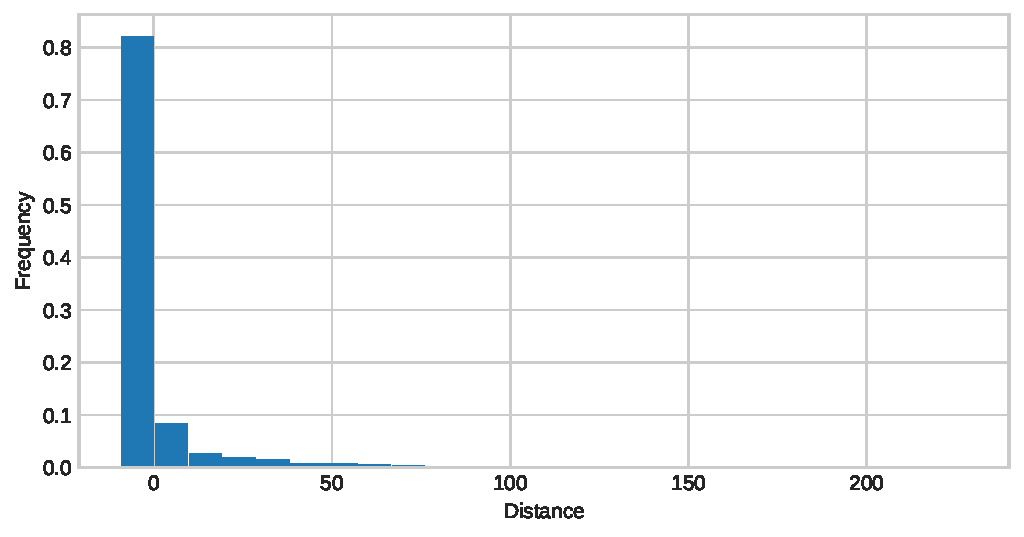
\includegraphics[width=.85\textwidth]{evaluation-results/figures/distance-distribution-histogram-Geometric-25.pdf}
    \caption{Matched segments geometric distance distribution histogram (binning=25)}
    \label{fig:distance-distribution-histogram-Geometric-25}
    \end{figure}

    In the current evaluation, the geometric distance between corpus and parser segments spans from a minimum 0 to maximum 219 characters. The mean distance is 4.99, which is close to the minimum point, with a standard deviation of 14.67, which, in relative terms, indicates an extreme deviation of 2940\%. The skew over 1 indicates a strong asymmetry to the right, and the kurtosis of 43.14 (almost 15 times the threshold of 3) indicates that most of the data, about 80\%, gravitate towards the left, between 0 and slightly over the mean, while the rest of the data point continue into a very long tail to the right. This is depicted in Figure \ref{fig:distance-distribution-histogram-Geometric-25}. 
    
    As appears in Figure \ref{fig:distance-distribution-histogram-Geometric-25}, the data follow a power law distribution \citep{newman2005power}. Here 62\% are not shifted at all and 83\% of the segments are slightly shifted up to 5 characters. There rest (27\%) of the segments are shifted by more than 5 characters. These ratios approximate Patetto's 80-20 distribution law but may as well fit Zipf's law \citep{newman2005power}. In future work, properties of these data should further be analysed, including the distribution fitting, that is selection of the theoretical distribution that fits best to a dataset.
    
    \begin{figure}[!ht]
    \centering
    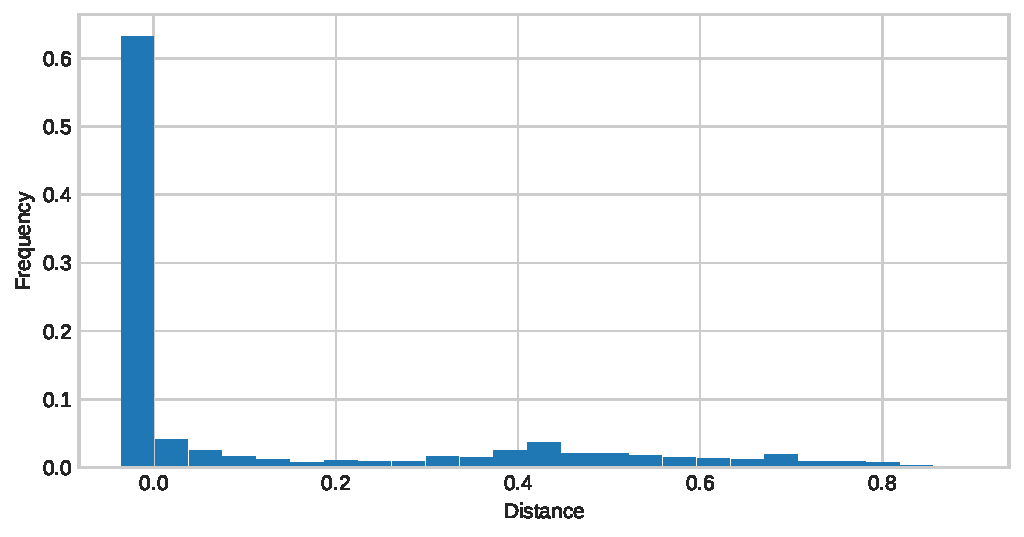
\includegraphics[width=.85\textwidth]{evaluation-results/figures/distance-distribution-histogram-WindowDiff-25.pdf}
    \caption{Matched segments WindowDiff distance distribution histogram (binning=25)}
    \label{fig:distance-distribution-histogram-WindowDiff-25}
    \end{figure}
    
    Next distance that I discuss is WindowDiff distance between corpus and parser segments. One crucial difference to geometric distance is the normalisation to [0,1] interval. In the current evaluation, the WindowDiff distance distribution, depicted in Figure \ref{fig:distance-distribution-histogram-WindowDiff-25}, spans from a minimum 0 to maximum score of 0.86. The mean distance is 0.15 with a standard deviation of 0.23 i.e. $\pm$159\%. The mean value is close to the minimum point, the relative standard deviation indicated extreme deviations of 159\%, the skew over 1 indicates a strong asymmetry to the right, and the kurtosis of 0.28 indicate the distribution does not have many outliers in the tail. 
    
    One positive aspect of this distance distribution is that the tail is not so long due to its normalised structure. This permits aggregation of the outliers we have observed in geometric distance distribution into a compact spectrum. This way, kurtosis, which, in this case, is smaller than 3, no longer indicates an abnormally long tail of outliers. 
    
    The histogram in Figure \ref{fig:distance-distribution-histogram-WindowDiff-25} resembles a power law distribution and more analysis work needs to be done in the future, including the distribution fitting and relation to the causes of partial matches in the first place. 
    
    This section presented the segmentation evaluation and distance analysis of the partially matching segments. The data show that the parser generates segments exactly as provided in the corpus with an accuracy of 0.71, and segments that partially correspond to those in the corpus with an accuracy of 0.8. We will see in the next sections that this partial match is supported by the identical labels that the segments carry. The distances of the partially matched segments, in about 80\% of the cases do not exceed 5 characters, but can span, most probably by mistake, over 200 characters. Next I move on to present the evaluation of the segment label assignments, which in our case are unit classes and functions.

\subsection{Unit class evaluation}
\label{sec:unit-class-evaluation}
    In this and the next section I present the parser syntactic accuracy. The syntactic accuracy aims to measure how well the main unit types and the clause main elements have been detected by the parser compared to the corpus. The evaluation is performed on the OCD corpus. This evaluation is restricted to the clause and four group types: nominal, prepositional, adverbial and adjectival. No clause complexes, group complexes or word types are included. The evaluation data are depicted in Figure \ref{fig:unit-types-data}. The names of the unit classes are provided on the x axis at the bottom of the graph while on the y axis the absolute number of occurrences is provided. 
    
    The meaning of exact and close match has been explained in Section \ref{sec:segmentation-evaluation} and from now on the label ``Matched'' will mean the segments that are either exactly or closely matched all together, while the label with a remark ``(exact only)'' means that it applies to only the portion of the exactly matched segments. 
    
    
    \begin{figure}[!ht]
    \centering
    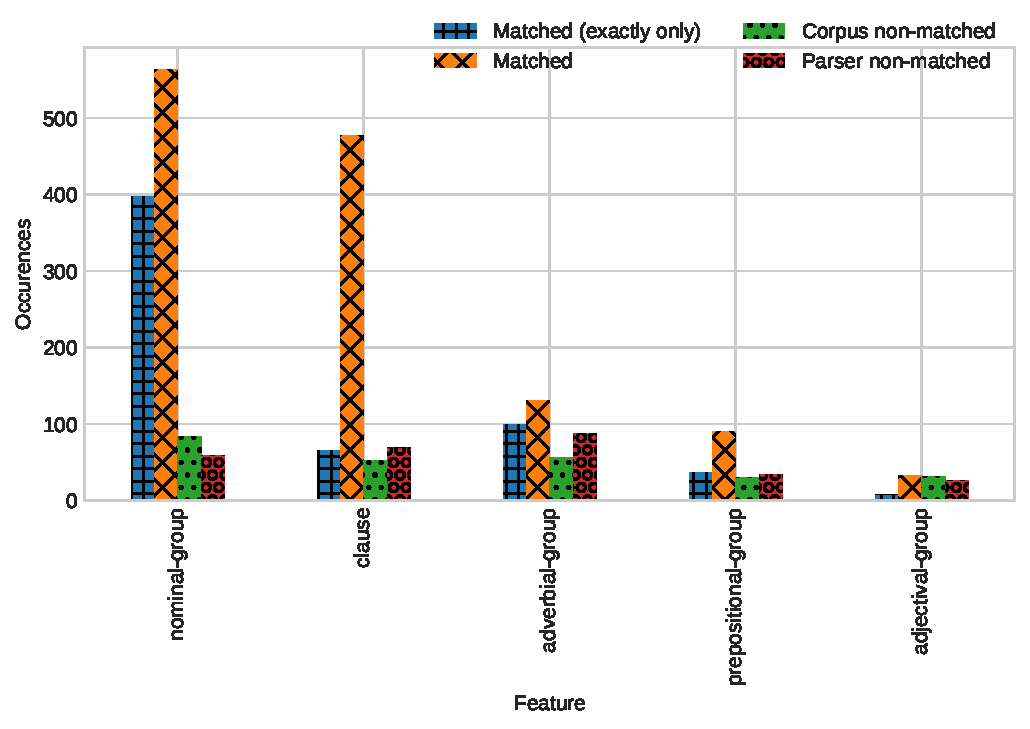
\includegraphics[width=.85\textwidth]{evaluation-results/figures/unit-types-data.pdf}
    \caption{Bar chart of matched and non-matched segments for the main unit classes}
    \label{fig:unit-types-data}
    \end{figure}
    
    To make the data easier to read and interpret I present the evaluation data in a table form using relative values to the number of matched segments. The absolute values of the evaluation statistics are contained in the graphical form and also available in the appendices in the table form. The relative evaluation data in this and the following sections will be presented in tables with the same structure. Using Table \ref{tab:unit-types-relative} as example, the column meaning is as follows. The first column contains the name of the unit class, element or feature. The column ``Matched'' contains the absolute number of matched segments with a specific label. The three other columns represent the number of segments relative to the ``Matched'' ones. So the column ``(\%) Matched (exactly only)'' means that out of all the matched segments that many represent exact matches and the rest to 100\% are partially matched segments. The column ``(\%) Corpus non-matched'' represent the number of segments relative to the total number of segments of particular type in the corpus, which remain unmatched. The column signifies the fraction of segments that remain unmatched, while the rest up to 100\% have, each, a corresponded in the parser output. The column ``(\%) Parser non-matched'' represents the number of segments (relative to the total number of segments of particular type in the parser output) in the parser output that do not have a correspondent in the corpus.
    
    \begin{table}[!ht]
    \centering
    \begin{tabulary}{\textwidth}{lCCCC}
    \toprule
    {} &  Matched &  (\%) Matched (exactly only) &  (\%) Corpus non-matched &  (\%) Parser non-matched \\
    \midrule
    nominal-group       &   564.00 &                       70.39 &                   12.96 &                    9.47 \\
    clause              &   477.00 &                       13.84 &                    9.83 &                   12.64 \\
    adverbial-group     &   131.00 &                       76.34 &                   29.95 &                   40.18 \\
    prepositional-group &    90.00 &                       41.11 &                   25.00 &                   27.42 \\
    adjectival-group    &    33.00 &                       24.24 &                   49.23 &                   44.07 \\
    \bottomrule
    \end{tabulary}
    \caption{The evaluation statistics relative to the number of matched segments for the main unit classes}
    \label{tab:unit-types-relative}
    \end{table}
    
    The evaluation data from Table \ref{tab:unit-types-relative} indicate that most (over 70\%) of the nominal and adverbial groups are identified with exact same borders as in the corpus while clause borders exhibit the most disagreement reflected by their low score of exact matches, only 13.84\%. The proportion of unmatched unit class segments in both the corpus and parser output varies between 9\% for clauses and nominal groups, and over 40\% for adjectival and adverbial groups. These proportions, however, are better interpreted when they are embedded into precision and recall score, which are provided in Table  \ref{tab:unit-types-combined-F1}. 
    \begin{table}[!ht]
    \centering
    \begin{tabular}{lcccccc}
    \toprule
     & \multicolumn{3}{c}{Exact match only} & \multicolumn{3}{c}{Exact and close match} \\ \cline{2-7} 
     & Precision & Recall & F1 & Precision & Recall & F1 \\ 
    \midrule
    nominal-group & 0.87 & 0.83 & 0.85 & 0.91 & 0.87 & 0.89 \\
    adverbial-group & 0.53 & 0.64 & 0.58 & 0.87 & 0.90 & 0.89 \\
    prepositional-group & 0.52 & 0.55 & 0.54 & 0.73 & 0.75 & 0.74 \\
    clause & 0.49 & 0.56 & 0.52 & 0.60 & 0.70 & 0.65 \\
    adjectival-group & 0.24 & 0.20 & 0.22 & 0.56 & 0.51 & 0.53 \\ 
    \bottomrule
    \end{tabular}
    \caption{Parser accuracy statistics for for the main unit classes}
    \label{tab:unit-types-combined-F1}
    \end{table}
    
    The scores provided in the first three columns are calculated with respect to exact matches only, which can be seen reflected in the lower precision, recall and $F_1$ scores when compared to their correspondents in the last three columns. These scores, nonetheless, constitute an appropriate baseline for comparing parser accuracy for when the close matches are considered as well. Note that in all cases of a match, close or exact, the segments bear the same label, and so, as explained in Section \ref{sec:differences}, the source of the divergence is in the segmentation. 
    
    The last three columns in Table \ref{tab:unit-types-combined-F1} show that clause and normal group units are identified with almost 0.9 $F_1$ measure, which is an encouraging result, while the adjectival and adverbial groups score 0.53 and 0.65 indicates that there is some space for improvement. 
    Further investigation is needed to discover the reason for the lower scores as there seem to be no obvious cause other than corpus and/or parser errors. Also, as visible in Figure \ref{fig:unit-types-data}, there is a contrast in the number of segments between the first two unit types and the last three with a ratio of one to four or more. The low number of exemplars in this evaluation contributes to a certain extent to the lower accuracy statistics.
    
\subsection{Clause Mood elements evaluation}
\label{sec:unit-mood-element-evaluation}

    In this section I describe the evaluation statistics reflecting the parser capacity to detect the main elements of a clause. The data available in the corpus unfortunately does not permit to evaluate units of lower rank such as nominal, prepositional, adjectival and other groups. Next I present statistics on the clause Mood elements, which were described in Chapter \ref{ch:the-grammar}. These elements are present in the annotations of the OCD corpus as explained in the beginning of this chapter in Section \ref{sec:corpus}. 
    
    \begin{figure}[!ht]
    \centering
    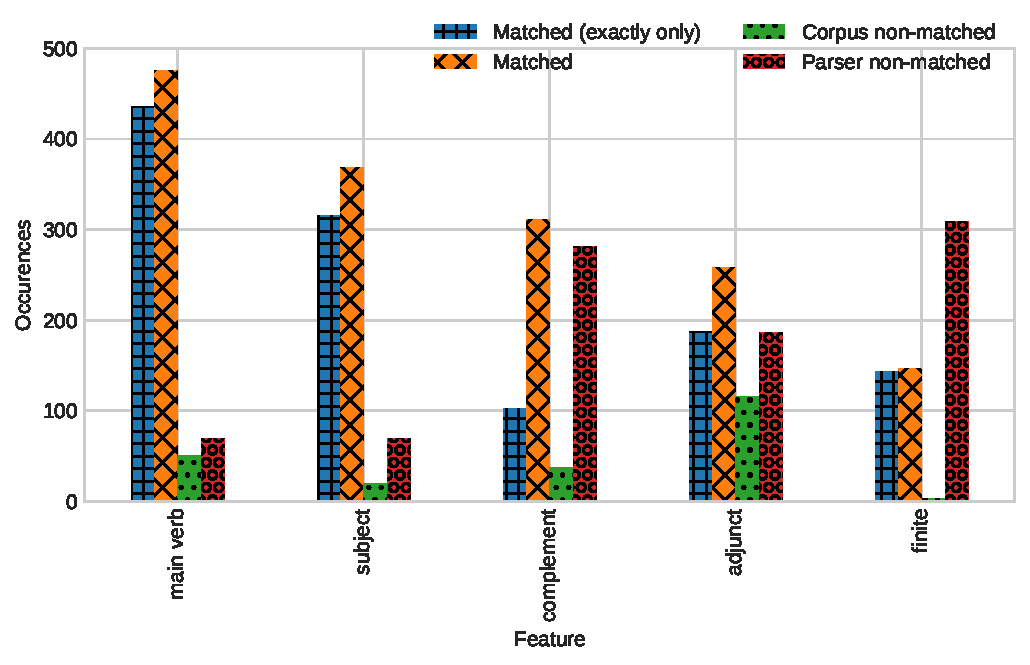
\includegraphics[width=.85\textwidth]{evaluation-results/figures/unit-elements-mood-data.pdf}
    \caption{Bar chart of matched and non-matched segments for the clause main Mood elements}
    \label{fig:unit-elements-mood-data}
    \end{figure}
    
    The OCD corpus annotations provide with the main syntactic (Mood) elements in the clause. Some of them, such as Auxiliary verbs, Main verb extension, Negation particle, and others have been omitted in the corpus and are thus missing in the present evaluation. Figure  \ref{fig:unit-elements-mood-data} reflects the absolute values from the empirical data. 
    
    The parser accuracy measurements for syntactic are contained in Table \ref{tab:unit-elements-mood-combined-F1}. The $F_1$ score for subjects and main verbs is nearly 0.9 while the complements and adjuncts are over 0.6. Finite element scores nearly 0.5 which is a low score for such easy to detect element. The reason for it lays in the incomplete corpus annotations, which fails to account for conflation of the finite and main verb elements. So when there was a main verb that was also a finite, only the main verb function was marked, which is incomplete. This incompleteness is also reflected in the discrepancy between low precision of 0.32 and high recall of 0.98. 
    
    \begin{table}[!ht]
    \centering
    \begin{tabular}{lcccccc}
    \toprule
     & \multicolumn{3}{c}{Exact match only} & \multicolumn{3}{c}{Exact and close match} \\ \cline{2-7} 
     & Precision & Recall & F1 & Precision & Recall & F1 \\ 
    \midrule
    main verb & 0.86 & 0.90 & 0.88 & 0.87 & 0.90 & 0.89 \\
    subject & 0.82 & 0.94 & 0.88 & 0.84 & 0.95 & 0.89 \\
    complement & 0.27 & 0.73 & 0.39 & 0.53 & 0.89 & 0.66 \\
    adjunct & 0.50 & 0.62 & 0.55 & 0.58 & 0.69 & 0.63 \\
    finite & 0.32 & 0.98 & 0.48 & 0.32 & 0.98 & 0.49 \\
    \bottomrule
    \end{tabular}
    \caption{Parser accuracy statistics for the clause main Mood elements}
    \label{tab:unit-elements-mood-combined-F1}
    \end{table}
    
    The number of complements unmatched in the parser output is nearly the same as the number of matched complements. This is reflected in the 0.53 precision score and nearly 0.9 recall rate which overall lead to an $F_1$ score lower than that of subject and main verb elements. This can be explained by a flaw, mentioned in Section \ref{sec:corpus}, in the annotation methodology as follows. The clausal complements often were annotated as a new clauses omitting to draw the same segment and marking it to be a complement in the clause above. This required the corpus revision and correction. Adjuncts however have a higher number of unmatched segments on both sides and this may be due to bugs in the parser and other mistake or omissions in the corpus.
    
\subsection{Clause Transitivity elements evaluation}
\label{sec:unit-transitivity-element-evaluation}

    OE corpus, provides with elements needed in semantic (Transitivity) parsing. The employed elements are Configuration, Participant role and Main verb while Circumstances are excluded from the study. Figure \ref{fig:unit-elements-transitivity-data} summarises the evaluation data. 
    
    The configuration segments, in SFG, correspond to clause segments, the participant role segments have as correspondents either the subject or complement segments, while the Main verb segments are shared. The aggregation of Subjects and Complements can be observed in Figure \ref{fig:unit-elements-transitivity-data} where the number of participant roles is approximately double the number of configurations. A configuration can have between one and three participants, and current data show an average of two participants per clause. 
    
    \begin{figure}[!ht]
    \centering
    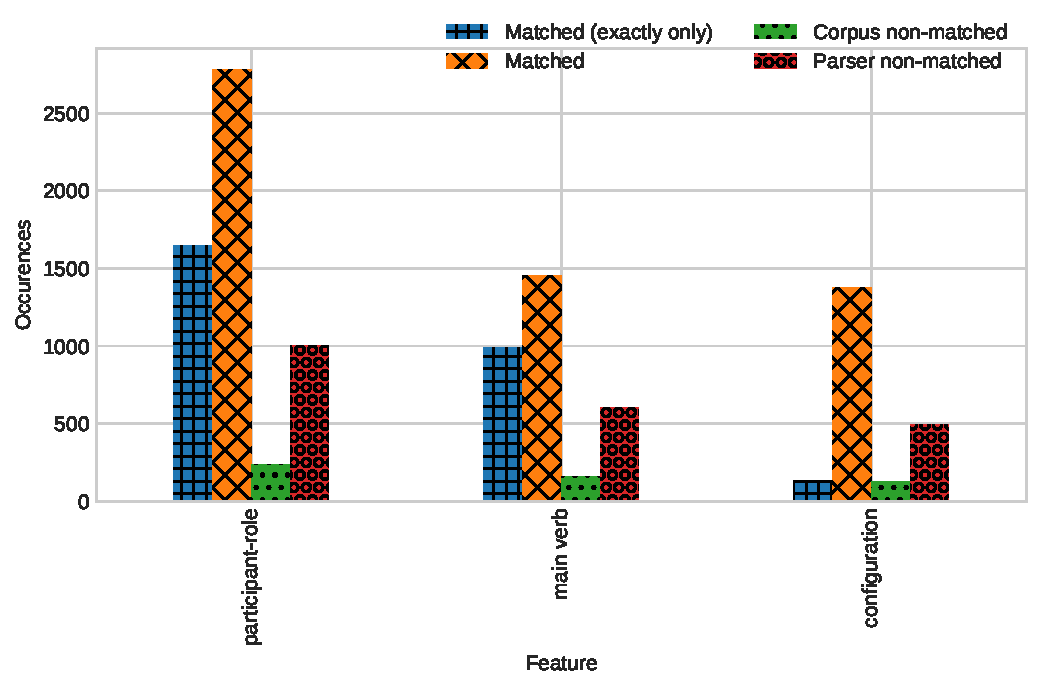
\includegraphics[width=.85\textwidth]{evaluation-results/figures/unit-elements-transitivity-data.pdf}
    \caption{Bar chart of matched and non-matched segments for the clause main Transitivity elements}
    \label{fig:unit-elements-transitivity-data}
    \end{figure}
    
    Note that in Figure \ref{fig:unit-elements-transitivity-data} the scale stretches over 2500 which reflects a much larger number of segments in OE corpus than that available in the OCD corpus. This, and certainly a higher quality of annotations, is reflected in the fairly uniform evaluation results. The $F_1$ (0.82), precision (0.74) and recall (0.92) scores vary very little across elements when compared to scores of the syntactic elements shown in Table \ref{tab:unit-elements-mood-combined-F1},  which vary substantially from one element to another.   

    \begin{table}[!ht]
    \centering
    \begin{tabular}{lcccccc}
    \toprule
     & \multicolumn{3}{c}{Exact match only} & \multicolumn{3}{c}{Exact and close match} \\ \cline{2-7} 
     & Precision & Recall & F1 & Precision & Recall & F1 \\ 
    \midrule
    participant-role &       0.62 &    0.88 & 0.73 &       0.74 &    0.92 & 0.82 \\
    configuration    &       0.22 &    0.52 & 0.30 &       0.74 &    0.92 & 0.82 \\
    main verb        &       0.62 &    0.86 & 0.72 &       0.71 &    0.90 & 0.79 \\ 
    \bottomrule
    \end{tabular}
    \caption{Parser accuracy statistics for the clause main Mood elements}
    \label{tab:unit-elements-transitivity-combined-F1}
    \end{table}
    
    In case of exact match evaluation the scores are lower for participant roles and main verbs, situating at 0.73 $F_1$ value, while configuration $F_1$ plummeted to 0.3. As configurations correspond in SFG to clauses boundary establishment methodology plays a significant role in achieving exact matches. Thus the discrepancy in the $F_1$ score between exact and combined matches is explainable by a discrepancy in the clause boundaries establishment and was already addressed in Section \ref{sec:differences}. 
    
    We come to the end of the syntactic structure evaluation where I have shown that the parser segments text exactly as in the corpus with an accuracy of 0.7 and an approximately same segmentation with an accuracy of 0.8. The parser detects unit classes on average with a score of 0.52 $F_1$ for exact matches and 0.74 $F_1$ for close matches. The Mood and Transitivity elements are detected on average with a 0.71 and 0.81 $F_1$ scores. 
    
    A constituency parser that generates a syntactic analysis using comparable unit classes and functions (using phrase structure grammars) such as for example \citet{chen2014fast}, \citet{stern2017minimal} or \citet{kitaev2018multilingual} reach an accuracy of 0.95 $F_1$ for English. This state of the art in parsing with other grammars reflects that there is a large space to improve the accuracy of Parsimonious Vole constituency. But it should not be separated from the main mission of this work to parse with constituency structures enriched with features from system networks. Next I present the evaluation of the the systemic feature selections from the MOOD and from the TRANSITIVITY system networks. 

    
    
\section{Evaluation of the systemic features assignment}
\label{sec:systemic-evaluation}
    In this section ... 
    % todo: 
    
    % todo say that the exact and close matches no longer play a role in the evaluation because it is about the features assigned to the unit and is of paradigmatic nature, thus has nothing to do with the syntagmatic dimension where the segments live :) 
    
\subsection{Evaluation of the MOOD systemic features assignment}
\label{sec:systemic-evaluation-MOOD}

    In this section I present the evaluation results for the systemic selections from the MOOD system network assigned to units in the constituency structure. The fragment of the MOOD system network used in this evaluation was presented as part of the OCD corpus description in Section \ref{sec:corpus}. The parser provides more feature selections as described in Section \ref{sec:mood} of the chapter describing the parser grammar, but the current evaluation is limited to only what is available in the corpus.

    In Table \ref{tab:features-mood} are provided the evaluation results for each of the MOOD features grouped by system network. On average the parser assigns systemic features with a precision of 59\%. I do not address the evaluation of every feature in part but analyse the results as a whole taking a few systems as examples for discussion. Addressing each system in part aiming at understanding why the score is satisfactory of not should be tackled in future work.

     \begin{table}[!ht]
        \centering
        \resizebox{0.8\textwidth}{!}{%
            \begin{tabulary}{1.1\textwidth}{@{}lCCCccc@{}}
            \toprule
             & Match & Corpus non-matched & Parser non-matched & Precision & Recall & F1 \\ \midrule
            POLARITY-TYPE &  &  &  &  &  &  \\
            positive & 485 & 125 & 55 & 0.90 & 0.80 & 0.84 \\
            negative & 57 & 10 & 70 & 0.45 & 0.85 & 0.59 \\
            VOICE-TYPE &  &  &  &  &  &  \\
            active & 553 & 102 & 68 & 0.89 & 0.84 & 0.87 \\
            passive & 11 & 11 & 28 & 0.28 & 0.50 & 0.36 \\
            FINITNESS &  &  &  &  &  &  \\
            non-finite & 99 & 19 & 38 & 0.72 & 0.84 & 0.78 \\
            finite & 526 & 33 & 554 & 0.49 & 0.94 & 0.64 \\
            NON-FINITE-TYPE &  &  &  &  &  &  \\
            perfective & 71 & 12 & 16 & 0.82 & 0.86 & 0.84 \\
            imperfective & 26 & 9 & 24 & 0.52 & 0.74 & 0.61 \\
            DEICTICITY &  &  &  &  &  &  \\
            temporal & 446 & 74 & 55 & 0.89 & 0.86 & 0.87 \\
            modal & 12 & 33 & 6 & 0.67 & 0.27 & 0.38 \\
            MOOD-ASSESSMENT-TYPE &  &  &  &  &  &  \\
            temporality & 35 & 17 & 27 & 0.56 & 0.67 & 0.61 \\
            modality & 15 & 32 & 8 & 0.65 & 0.32 & 0.43 \\
            intensity & 12 & 14 & 43 & 0.22 & 0.46 & 0.30 \\
            MOOD-TYPE &  &  &  &  &  &  \\
            indicative & 455 & 216 & 37 & 0.92 & 0.68 & 0.78 \\
            imperative & 4 & 1 & 31 & 0.11 & 0.80 & 0.20 \\
            INDICATIVE-TYPE &  &  &  &  &  &  \\
            declarative & 355 & 260 & 27 & 0.93 & 0.58 & 0.71 \\
            interrogative & 47 & 7 & 63 & 0.43 & 0.87 & 0.57 \\
            INTERROGATIVE-TYPE &  &  &  &  &  &  \\
            wh & 40 & 6 & 57 & 0.41 & 0.87 & 0.56 \\
            yes-no & 5 & 3 & 8 & 0.38 & 0.62 & 0.48 \\
            WH-SELECTION &  &  &  &  &  &  \\
            wh-subject & 9 & 3 & 7 & 0.56 & 0.75 & 0.64 \\
            wh-adjunct & 11 & 15 & 3 & 0.79 & 0.42 & 0.55 \\
            wh-complement & 8 & 0 & 62 & 0.11 & 1.00 & 0.21 \\ \bottomrule
            \end{tabulary}
        }
        \caption{The evaluation statistics available for the MOOD system network}
        \label{tab:features-mood}
    \end{table}
    
    Table \ref{tab:features-mood} summarises the evaluation results for the MOOD system network features grouped by system name marked with capital letters. The order in which the features appear in the table follow roughly an increase in systemic delicacy. As delicacy increases there are increasingly fewer occurrences where a system is employed. This is also associated also by a decrease in accuracy although there are multiple factors influencing it among which corpus quality and small population size. 
    
    The precision and recall values vary quite a lot from a minimum of 11\% up to a maximum of 93\% and the harmonic mean, the $F_1$ score, between 30\% and 87\%  averaging to almost 60\%. The details can be read in Table \ref{tab:mood-accuracy}. The distribution of these values can be seen in Figures \ref{fig:mood-precission-recall} and \ref{fig:mood-precission-f1}. A noticeable feature is the presence of two peaks in the precision and recall distributions: one around 50\% and the other one around 90\%. They translate into a similar $F_1$ distribution with peaks at 60\% and 85\%, a phenomena which I address next.

    \begin{table}[!ht]
        \centering
        \begin{tabular}{lccc}
            \toprule
            {} & {Precision} & {Recall} & {F1} \\ %\hline
            % feature count & 21.00 & 21.00 & 21.00 \\ \hline
            \midrule
            mean & 0.57 & 0.73 & 0.59 \\ 
            standard deviation & 0.27 & 0.18 & 0.21 \\ 
            min value & 0.11 & 0.32 & 0.20 \\ %\hline
            25\% quantile & 0.41 & 0.62 & 0.48 \\ %\hline
            50\% quantile & 0.56 & 0.80 & 0.61 \\ %\hline
            75\% quantile & 0.82 & 0.86 & 0.78 \\ %\hline
            max value & 0.93 & 1.00 & 0.87 \\ %\hline
            \bottomrule
        \end{tabular}
        \caption{Descriptive statistics of the precision, recall and F1 scores for evaluated MOOD features}
        \label{tab:mood-accuracy}
    \end{table}

    Within most systems, the $F_1$ scores exhibit a contrast from one feature to the other. What this means is discussed in the next two cases. For example in the POLARITY-TYPE system the positive polarity feature scores 84\% $F_1$ measure and negative one almost 60\%. As per Definition \ref{def:system}, the system features are mutually exclusive. The polarity of an English clause is positive by default unless a negation marker is found and this represents only 10\% of the clauses in  the corpus. This means that it should be sufficient for the parser to detect one feature with a reasonably high $F_1$ score then the converse feature should be detectable with the same degree of accuracy. Yet the current data invalidate this hypothesis as the grammar does not represent exclusivity.
    
    \vspace{1em}
    \noindent
    \begin{minipage}[t]{0.49\textwidth}
        \centering
        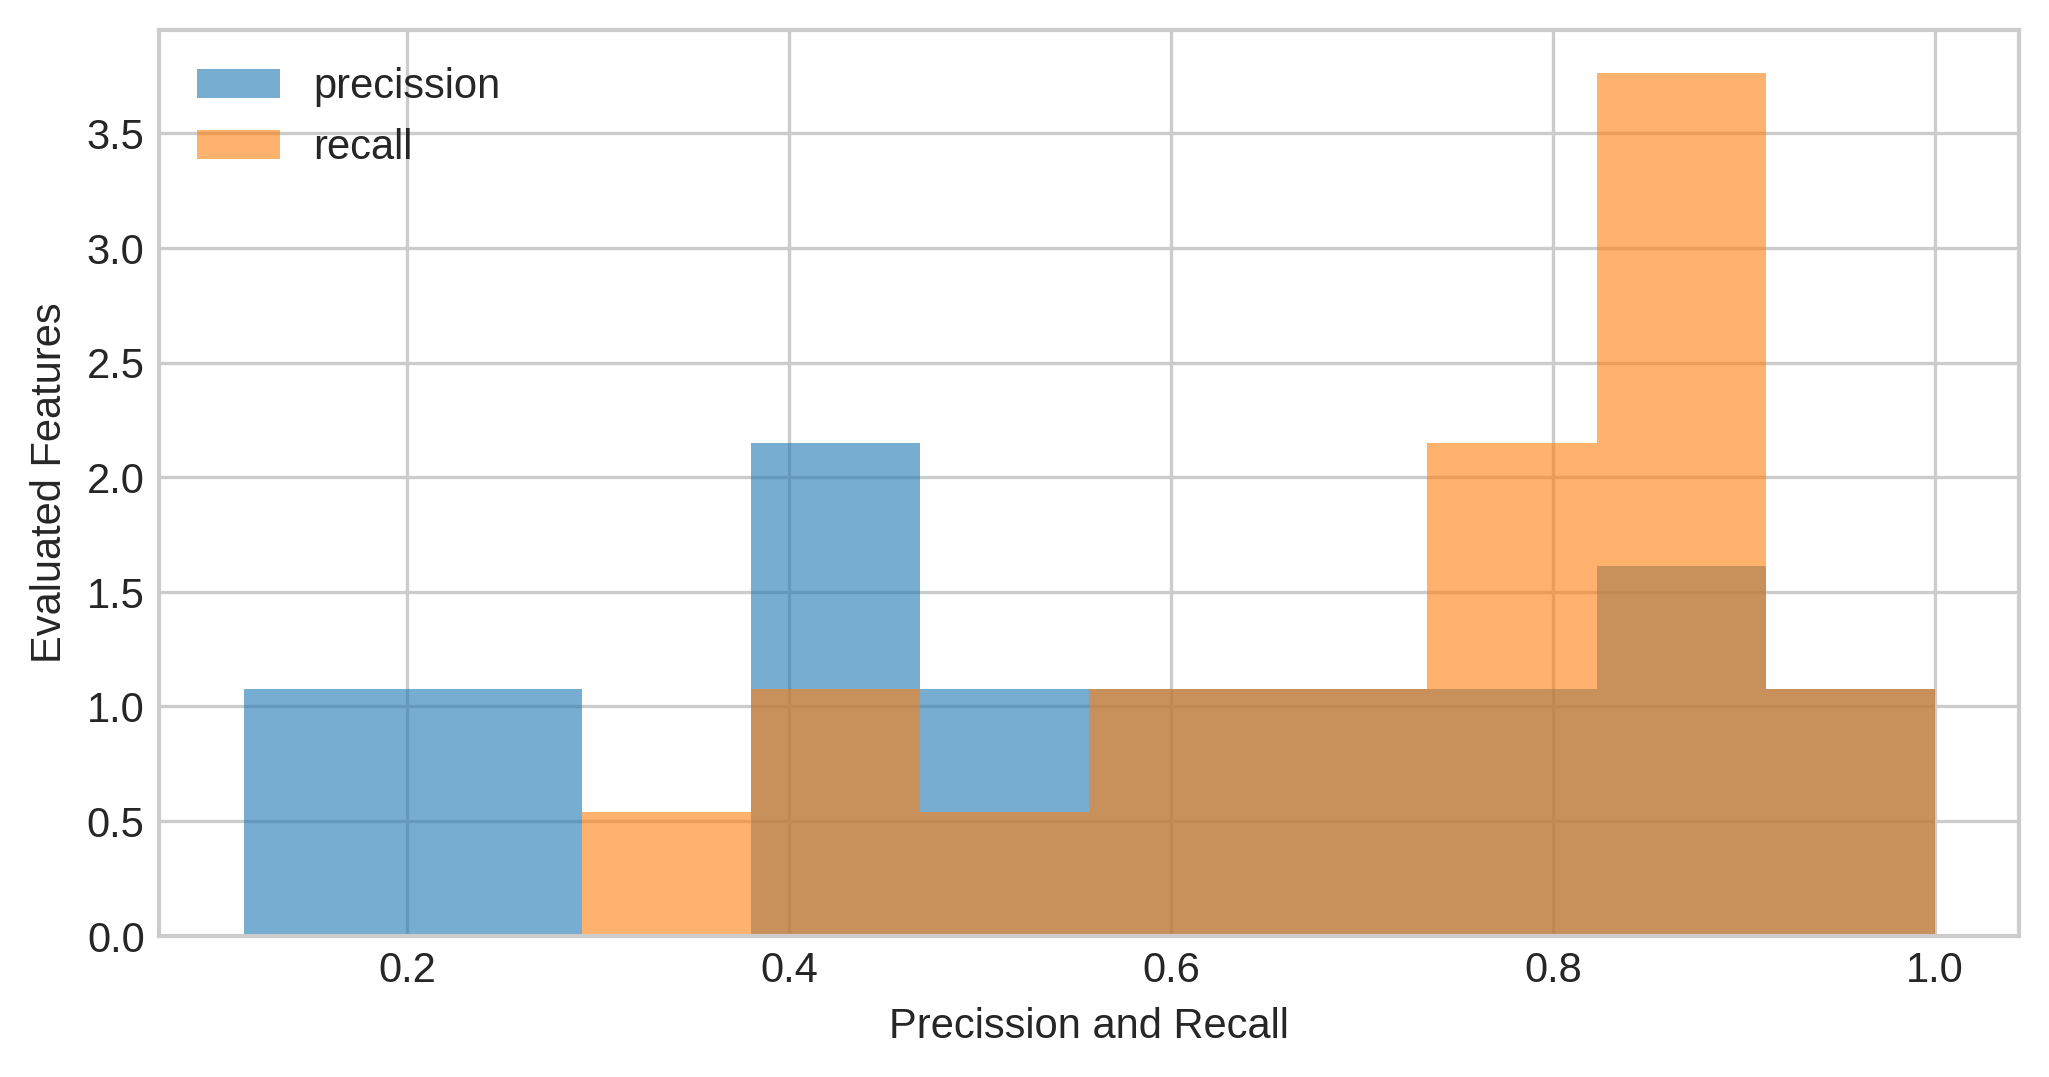
\includegraphics[width=\textwidth]{evaluation-results/figures-old/accuracy-syntactic-mood-precission-recall.png}
        \captionof{figure}{The distribution of precision and recall for selected features from the MOOD system network}
        \label{fig:mood-precission-recall}
    \end{minipage}
    \quad
    \begin{minipage}[t]{0.49\textwidth}
        \centering
        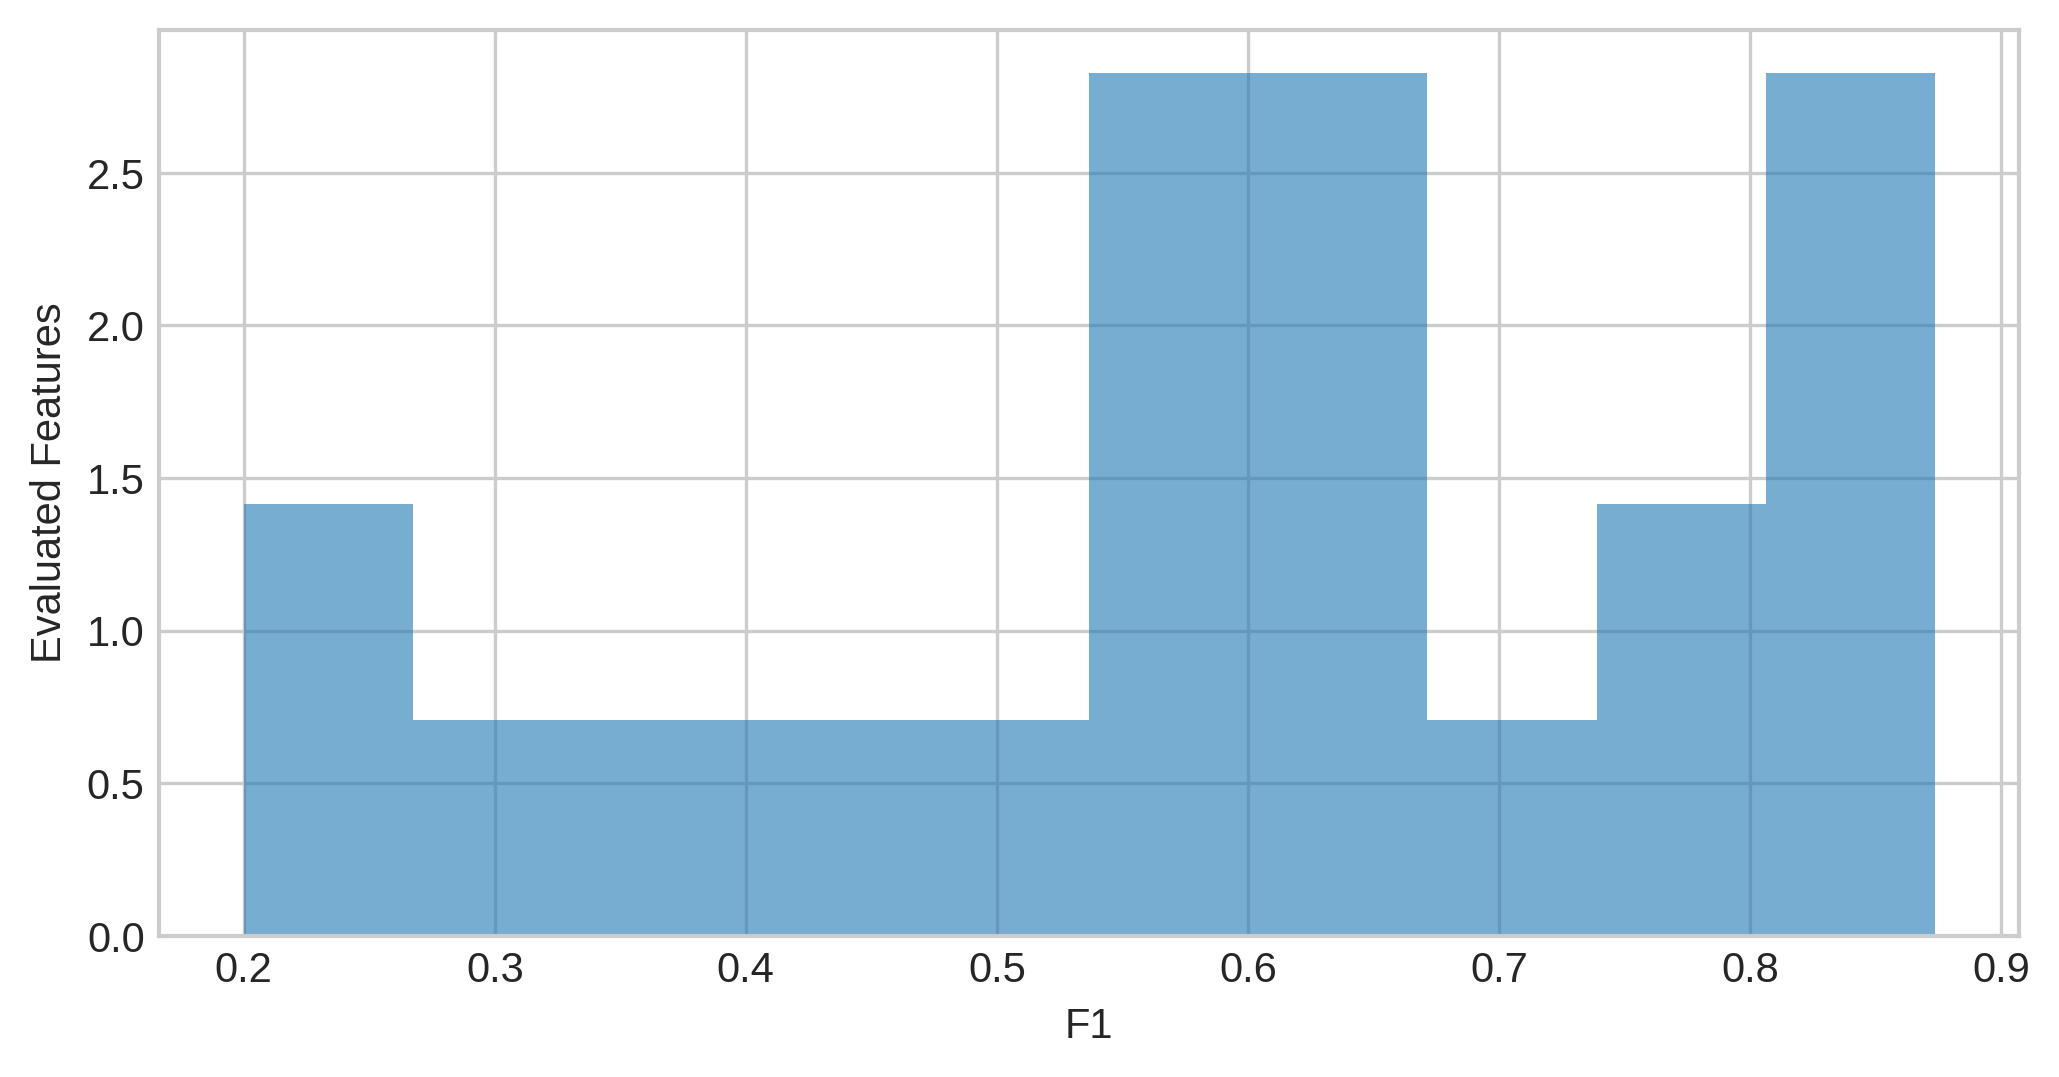
\includegraphics[width=\textwidth]{evaluation-results/figures-old/accuracy-syntactic-mood-f1.png}
        \captionof{figure}{The distribution of F1 score for selected features from the MOOD system network}
        \label{fig:mood-precission-f1}
    \end{minipage}
    \vspace{1em}
    
    In the case of the POLARITY-TYPE system, the phenomena may be explained as a consequence of low delicacy in the parsing algorithm. The current implementation determines polarity by checking for the presence of the negation verbal marker only. Nonetheless a more delicate polarity testing will have to take into consideration polarity indicators from the subject, complement and adjuncts of various types that may have been taken into consideration during the annotation process. Providing an incomplete, less delicate implementation for systemic choices may be a source of errors and thus this hypothesis requires further investigation.  %The same can be expected of other systems that are reduced in delicacy 
    
    Nonetheless, the same phenomena can be seen if we look at the systems that do not span others with higher degrees of delicacy. For example, the detection mechanism for VOICE-TYPE is implemented similarly to POLARITY-TYPE. The parser checks whether there is a passive order of elements in the clause, otherwise the active voice is selected.  Detection of the positive voice scores a much higher $F_1$ measure of 87\% than the negative one of 36\%. There is no problem of low delicacy and still there is a discrepancy between the $F_1$ scores of the two features which is somewhat a surprising result. 

    One way to look at the high discrepancy between the feature accuracy scores can be as follows. 
    If we take VOICE-TYPE as example, most instances of active voice are easy to detect. But there is a portion of cases, regardless which voice it is, that are difficult for the parser to distinguish. The passive voice selections are executed mostly for these ambiguous cases. It it possible that this can be generalised to other system networks and more investigation is required to pinpoint exactly how such phenomena materialise.

    In future implementations we can take advantage of the mutual exclusivity of system features and capitalise on the above finding, at least for the leaf systems. Taking into consideration that the score of one feature is higher, clause elements should then be provided with selections of those features only, while the complement features, which score low in this evaluation should remain unassigned. This means that only features that can be provided with high confidence (using $F_1$ score as a measure of that) shall be assigned. Then an additional process can be implemented to select the remaining unassigned features. 
    
    % todo conclude this section

\subsection{Evaluation of the TRANSITIVITY systemic features assignment}
\label{sec:systemic-evaluation-TRANSITIVITY}
    
    In this section I present the evaluation of the TRANSITIVITY system network. As was explained in Section \ref{sec:corpus} above, the OE corpus contains annotations with the part from the original system network depicted in Figure \ref{fig:cardiff-transitivity}. The parser provides more feature selections as described in Section \ref{sec:transitivity} of the chapter describing the parser grammar, but the current evaluation is limited to only what is available in the corpus. 
    
    Transitivity analysis is semantic in nature and poses challenges in meaning selection beyond constituent class or function. The approach of assigning this sort of features was explained in Chapter \ref{ch:semantic-parsing}. Here I would like to remind an important aspect that impacts the evaluation results, explaining in some cases recall being higher than precision.
    
    In the grammar, described in Chapter \ref{ch:the-grammar}, a clause can be assigned a single process configuration and whose participant constituents can take only one role each. In the semantic role labelling task the situation is similar: a clause takes one semantic frame and each constituent only one semantic label. This means that a parser shall generate as output one semantic configuration that fits best the text. 
    
    The Parsimonious Vole parser does not always provide a single semantic configuration. Instead it generates one or several possible configurations for each clause instead of providing exactly a one. The reason for this is the mechanism by which semantic analysis is generated. The constituency structure is tested against a set of semantic graph patterns and the matching patterns enrich the constituency structure with semantic features immediately. In some cases more than one pattern matches the constituency structure leading to enrichment by multiple graph patterns, which is not entirely true. Thus these multiple assignments should be interpreted as alternating possibilities.  
    
    Intuitively, this should reduce recall on all the elements but the effects are mostly manifested at the level of participant roles as will be described below. First let's discuss the evaluation results for the process types, which are provided in Table \ref{tab:features-transitivity}, and after we will turn to the evaluation of participant roles.
    
    \begin{table}[!ht]
    \centering
    \resizebox{0.8\textwidth}{!}{%
        \begin{tabulary}{1.1\textwidth}{@{}lCCCccc@{}}
        \toprule
         & Match & Corpus non-matched & Parser non-matched & Precision & Recall & F1 \\ \midrule
        PROCESS-TYPE &  &  &  &  &  &  \\
        mental & 277 & 231 & 87 & 0.76 & 0.55 & 0.64 \\
        relational & 338 & 297 & 174 & 0.66 & 0.53 & 0.59 \\
        influential & 38 & 51 & 62 & 0.38 & 0.43 & 0.40 \\
        action & 170 & 231 & 352 & 0.33 & 0.42 & 0.37 \\
        event-relating & 1 & 28 & 0 & 1.00 & 0.03 & 0.07 \\
        RELATIONAL-TYPE &  &  &  &  &  &  \\
        attributive & 169 & 239 & 107 & 0.61 & 0.41 & 0.49 \\
        directional & 30 & 13 & 127 & 0.19 & 0.70 & 0.30 \\
        locational & 39 & 20 & 207 & 0.16 & 0.66 & 0.26 \\
        matching & 2 & 0 & 69 & 0.03 & 1.00 & 0.05 \\
        MENTAL-TYPE &  &  &  &  &  &  \\
        three-role-cognition & 45 & 51 & 34 & 0.57 & 0.47 & 0.51 \\
        two-role-cognition & 95 & 102 & 86 & 0.52 & 0.48 & 0.50 \\
        two-role-perception & 13 & 12 & 102 & 0.11 & 0.52 & 0.19 \\
        three-role-perception & 0 & 2 & 6 & 0.00 & 0.00 &  \\
        desiderative & 0 & 0 & 81 & 0.00 &  &  \\
        emotive & 0 & 0 & 87.00 & 0.00 &  & \\ \bottomrule
        \end{tabulary}
    }
    \caption{The evaluation statistics available for the PROCESS-TYPE system and few of its subsystems from the TRANSITIVITY system network}
    \label{tab:features-transitivity}
    \end{table}
    
    In Table \ref{tab:features-transitivity} \textit{mental} and \textit{relational} processes are the ones with highest $F_1$ scores: 0.64 and 0.59. They are followed by \textit{influential} and \textit{action} process types while results for the \textit{event-relating} are not conclusive because of the very small number of occurrences in the dataset. This can be read in Table \ref{tab:features-transitivity} where the number of matched segments is higher than the number of non matched corpus or parser segments. Note that considerable volume of annotations for process type sub-types are provided for mental and relational processes only \citep[153-155]{schulz2015me}.
    
    Among the \textit{mental} processes, \textit{two-role-cognition} and \textit{three-role-cognition} are parsed with highest accuracy of 51\% and 50\% correspondingly; whereas among \textit{relational} ones the \textit{attributive} process type scores the highest, 49\% while rest of them score much lower. This can be seen from the higher number of  non-matched segments for each process type for every feature.     
    
    \begin{table}[!ht]
    \centering
    \begin{tabular}{lccc}
        \toprule
        {} & {Precision} & {Recall} & {F1} \\ %\hline
        \midrule
        mean & 0.35 & 0.48 & 0.36 \\
        standard deviation & 0.32 & 0.26 & 0.19 \\
        min value & 0.00 & 0.00 & 0.05 \\
        25\% quantile & 0.07 & 0.42 & 0.24 \\
        50\% quantile & 0.33 & 0.48 & 0.39 \\
        75\% quantile & 0.59 & 0.55 & 0.51 \\
        max value & 1.00 (0.76) & 1.00 (0.70) & 0.64 \\
        \bottomrule
    \end{tabular}
    \caption{Descriptive statistics of the precision, recall and F1 scores for evaluated TRANSITIVITY features}
    \label{tab:transitivity-accuracy}
    \end{table}
    
    Looking at the entire set of evaluation results for process types, the precision and recall values vary quite a lot from a minimum of 3\% up to a maximum of 100\% and the harmonic mean, the $F_1$ score, between 7\% and 64\%  averaging to 41\%. The details can be read in Table \ref{tab:transitivity-accuracy}. The maximum of 100\% precision is a bit unfortunate because there is one instance of event-relating process found by the parser which also failed to find the other 28 thus the recall of 3\% only. So I decided to ignore this value and use the next maximum which is 76\% for mental process types. A similar case is for the matching process type which was provided only two times in the corpus but the parser generated 67 different instances of it.
    
    Next I provide an analysis of the evaluation data indicating a potential relation between the increase in the delicacy and effect it has on the parser accuracy. The accuracy of mental process detection is 64\% whereas the average accuracy for the mental sub-types (cognition, perception, desiderative and emotive) is 40\%. The same holds for relational process whose accuracy is 59\% whereas the average of its sub-types (attributive, directional, locational, matching) is only 26\%. I start by comparing the number of mental and relational segments to the sum of mental sub-type segments and sum of relational sub-type segments correspondingly. 
    
   \begin{table}[!ht]
    \noindent
    \resizebox{0.98\linewidth}{!}{%
     \begin{minipage}[t]{0.495\textwidth}
         \centering
         \resizebox{0.995\textwidth}{!}{%  
             \begin{tabulary}{1.2\textwidth}{|C|c|c|c|}
                 \hline
                 \textbf{Features} & \textbf{Manual} & \textbf{Parse} & \textbf{/} \\ \hline
                 mental & 508 & 364 & \textbf{0.72} \\ \hline
                 mental sub-types (sum of) & 320 & 549 & \textbf{1.72} \\ \hline
                 \textbf{/} & \textbf{0.63} & \textbf{1.51} &  \\ \hline
             \end{tabulary}
         }
         \caption{The ratios between \textit{mental} segments and the sum of mental sub-type segments}
         \label{tab:ratios-mental}
     \end{minipage}%
     \quad
     \begin{minipage}[t]{0.495\textwidth}
         \centering
         %    \begin{table}[!ht]
         \resizebox{0.995\textwidth}{!}{%  
             \begin{tabulary}{1.2\textwidth}{|C|c|c|c|}
                 \hline
                 \textbf{Features} & \textbf{Manual} & \textbf{Parse} & \textit{\textbf{/}} \\ \hline
                 relational & 635 & 512 & \textbf{0.8} \\ \hline
                 relational sub-types (sum of) & 512 & 750 & \textbf{1.47} \\ \hline
                 \textit{\textbf{/}} & \textbf{0.8} & \textbf{1.47} &  \\ \hline
             \end{tabulary}
         }
         \caption{The ratios between \textit{relational} segments and the sum of mental sub-type segments}
         \label{tab:ratios-relational}
         %    \end{table}
     \end{minipage}
     }
    \end{table}
    
    Table \ref{tab:ratios-mental} and \ref{tab:ratios-relational} provide each two pairs of ratios. They have very similar data content. Next I discuss the case of the mental process type only because the same applies to the case of relational processes and perhaps to other ones, but we lack data for testing this hypothesis. Thus, the first pair of ratios, provided in the lowest row, compares the number of segments with \textit{mental} feature to the sum of segments with any sub-type of \textit{mental} feature (i.e.  \textit{cognition}, \textit{perception}, \textit{emotive}, etc.). This ratio measures how well are the feature dependencies preserved across delicacy levels. The second pair of ratios, provided in the last column, compares the number of segments provided by the parser and to that available in corpus for both the mental feature and the sum of its sub-types.
    
    Table \ref{tab:ratios-mental} shows that in the corpus the number of segments with \textit{mental} feature is almost one fourth higher than what the parser provides (72 \%). This result means that probably not all the instances of a mental process have been detected by the parser (i.e. 28\% undetected). The same comparison ran on the sub-types of \textit{mental} process shows diametrically opposite results, i.e. three fourths more parser generated results than in the corpus (172\%) which is an indication of false positives. A possible explanation is the correlation between increase in delicacy and uncertainty i.e. the more delicate features are less precise in the parser results. As mentioned in the beginning of the section, uncertainty this case is manifested as a disjunction set of equally possible options. Currently there is no ranking available based on degrees of confidence. Hence the parser provides multiple feature selections from the same system (in this case MENTAL-TYPE) for the same constituent whereas there should be a single one. In the future this needs to be addressed by introducing a discrimination mechanism so that parser collects first all the possible matches and then only the most suitable is assigned possibly by using frequencies available from a corpus like OE.
    
    If we look again at Table \ref{tab:ratios-mental} and compare the number of all mental sub-type occurrences (see Figure \ref{fig:mental-types}) to the number of mental type occurrences, then we see that the ratio is quite low (63\%). As the delicacy of the features increases fewer of these features are provided in the corpus. This is a direct manifestation of difficulty in annotating with ever more delicate features. This ratio, therefore, measures the degree of incompleteness at this level of delicacy. Comparing the same ratio for the parser generated segments we notice an opposite result (151\%). This is in fact another measurement of noise generated due to uncertainty when advancing to a more delicate features as explained above. 
    
    \begin{table}[!b]
    \centering
    % \resizebox{0.8\textwidth}{!}{%
        \begin{tabulary}{0.8\textwidth}{@{}lCCCccc@{}}
        \toprule
        & Match & Corpus non-matched & Parser non-matched & Precision & Recall & F1 \\ 
        \midrule
        emoter & 91 & 70 & 57 & 0.61 & 0.57 & 0.59 \\
        phenomenon & 359 & 223 & 294 & 0.55 & 0.62 & 0.58 \\
        carrier & 267 & 263 & 244 & 0.52 & 0.50 & 0.51 \\
        cognizant & 82 & 84 & 104 & 0.44 & 0.49 & 0.47 \\
        agent & 267 & 210 & 428 & 0.38 & 0.56 & 0.46 \\
        possessed & 71 & 24 & 155 & 0.31 & 0.75 & 0.44 \\
        attribute & 162 & 241 & 170 & 0.49 & 0.40 & 0.44 \\
        affected & 93 & 70 & 663 & 0.12 & 0.57 & 0.20 \\
        \bottomrule
        \end{tabulary}
    % }
    \caption{The evaluation statistics available for the PARTICIPANT-ROLE-TYPE system from the TRANSITIVITY system network}
    \label{tab:features-participant-role-restricted}
    \end{table}
    
    So far we have discussed the process types and now let's turn attention towards the features from the PARTICIPANT-ROLE-TYPE system. Table \ref{tab:features-participant-role} presents the evaluation data along with the precision, recall and $F_1$ score for each participant role sorted according to $F_1$ score in descending order. 
    
    \begin{table}[!b]
    \centering
    \begin{tabular}{lccc}
        \toprule
        {} & {Precision} & {Recall} & {F1} \\ %\hline
        \midrule
        mean & 0.43 & 0.56 & 0.46 \\
        standard deviation & 0.16 & 0.10 & 0.12 \\
        min value & 0.12 & 0.40 & 0.20 \\
        25\% quantile & 0.37 & 0.50 & 0.44 \\
        50\% quantile & 0.46 & 0.56 & 0.46 \\
        75\% quantile & 0.53 & 0.58 & 0.53 \\
        max value & 0.61 & 0.75 & 0.59 \\
        \bottomrule
    \end{tabular}
    \caption{Descriptive statistics of the precision, recall and F1 scores for evaluated PARTICIPANT-ROLE features}
    \label{tab:features-participant-role-accuracy}
    \end{table}
    
    In this evaluation only the participant roles that appear at least 100 times in the corpus are considered. This restriction is inherited from \citet[160-162]{schulz2015me} study on OE corpus. The entire set of evaluation results for participant roles is provided in Table \ref{tab:features-participant-role} in Appendix \ref{ch:evaluation-data}. 
    
    The evaluation results for considered set of participant roles is summarised in Table \ref{tab:features-participant-role-accuracy}. The precision vary from 12\% to 61\% with an average of 43\%, and the recall values between 40\% and 75\% with an average of 56\%. The data is characterised by lower precision and higher recall. This is reflected in the $F_1$ score which is situated at a low average of almost 20\%. The maximum of 100\% recall is a bit unfortunate because there are three features with a single instance provided in the corpus and many provided in the parser output thus the precision of 0\%. So I decided to ignore this value and use the next maximum which is 75\% for possessed participant role.
    
    \vspace{1em}
    \noindent
    \begin{minipage}[b]{0.49\textwidth}
        \centering
        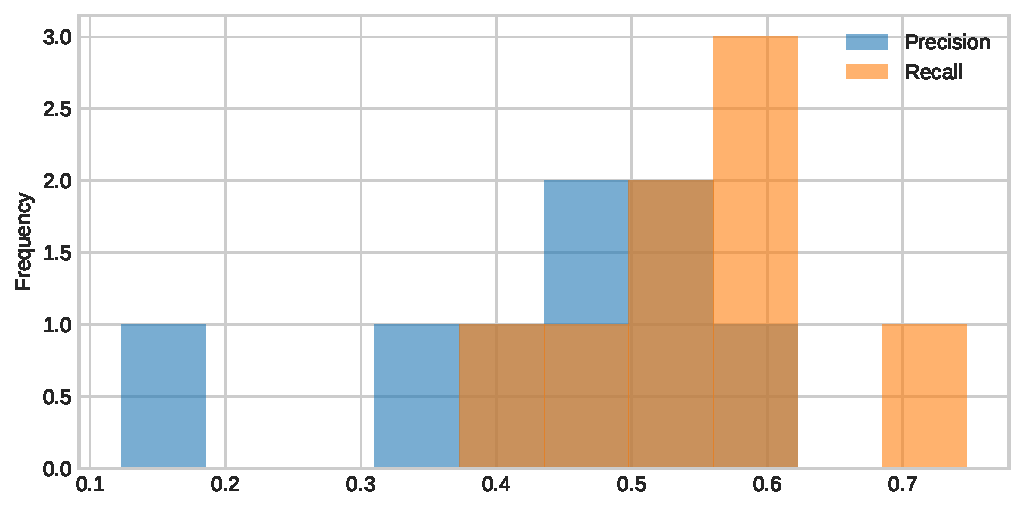
\includegraphics[width=\textwidth]{evaluation-results/figures/PARTICIPANT-ROLE-distribution-PR-10.pdf}
        \captionof{figure}{The distribution of precision and recall for selected features from the PARTICIPANT-ROLE system}
        \label{fig:participant-role-precission-recall}
    \end{minipage}
    \quad
    \begin{minipage}[b]{0.49\textwidth}
        \centering
        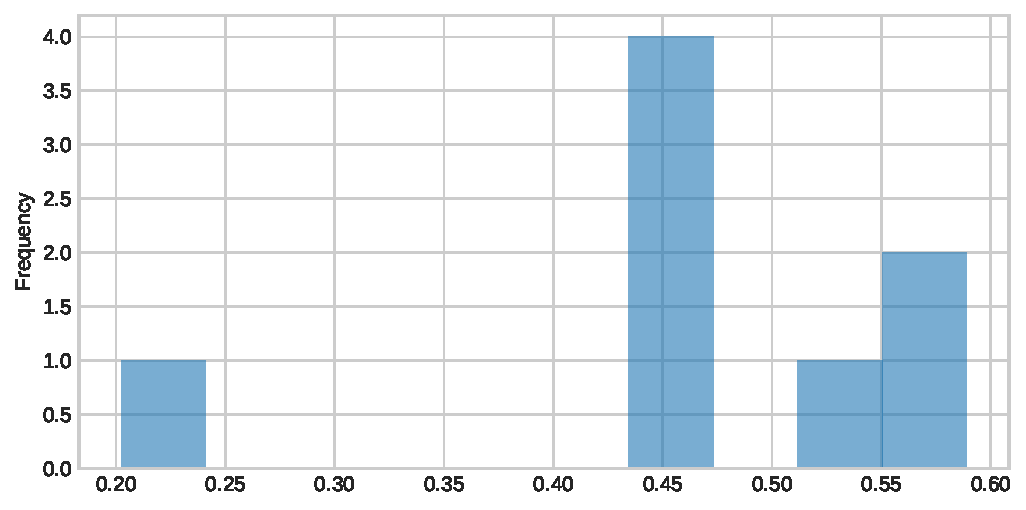
\includegraphics[width=\textwidth]{evaluation-results/figures/PARTICIPANT-ROLE-distribution-F1-10.pdf}
        \captionof{figure}{The distribution of F1 score for selected features from the PARTICIPANT-ROLE system}
        \label{fig:participant-role-precission-f1}
    \end{minipage}
    \vspace{1em}
    
     The distribution of precision, recall and $F_1$ scores can be seen in Figures \ref{fig:participant-role-precission-recall} and \ref{fig:participant-role-precission-f1}. The  noticeable feature is the high peak of precision near the minimum side of the graph and fairly uniform and flat distribution of recall up to the maximum side of the graph. They translate into $F_1$ distribution as three groups: a considerable first group near the minimum pole; a second small island, formed by destination and affected participant roles, at 20\% accuracy; and a third larger group between 40\% and 60\% accuracy on the right side of the graph.
    
    In Table \ref{tab:features-participant-role} a suite of eight features (emoter, phenomenon, carrier, possessive, cognizant, agent, possessed and attribute) have $F_1$ scores descending from almost 60\% to 44\%. Destination and affected features follow with half of the previous (20\%) and then the score halves again to 11\% continuing to descend towards zero. As the accuracy decreases we can notice that multiple features display high recall spikes. This is a manifestation of the assignment of multiple roles to the same participant for the reasons explained above for the process types. 

    From the data presented in Table \ref{tab:features-participant-role} we can conclude that only the first one third of the participant roles can be considered usable with a reasonable level of confidence. It also shows a serious lack of data for the lower one third of the participant roles, which is directly reflected in low precision scores. A hypothesis that I put forward here is that in a larger corpus, with broader coverage over the participant roles, the scores for the rare features would improve considerably compared to this results. The abnormally high number of participants generated by the parser must be addressed in future work starting with an investigation of the Transitivity graph patterns generated from the PTDB, in particular for the features exhibiting recall spikes. 
    
    The compound roles such as affected-carrier, affected-possessed, agent-perceiver etc. have scored very low accuracy especially if compared to their simple counter parts. For example carrier role is detected with an accuracy of 51\% and affected role with  20\% while the compound role with very low accuracy of only 7\%. This indicates that in future work the way compound roles are assigned by the parser and how these assignments are evaluated should be rethought and a different approach taken.  
    
    The next section concludes this evaluation chapter.
    % todo finish this section

\section{Discussion}
\label{sec:evaluation-discussion}
    
    In this chapter we have discussed how the empirical evaluation of Parsimonious Vole parser has been conducted. The stage is set through a general presentation of the corpora and what the task at hand is, i.e. identifying and comparing segments available in the manually annotated corpus to those generated automatically by the parser. The comparison is performed in terms of how accurate the spans of corpus and parser segments are and how many segments with the same label are matched.
    
    In Section \ref{sec:corpus} are presented the OCD and OE corpora that were used in the current evaluation exercise. OCD corpus is used for measuring the accuracy of the constituency structure and MOOD feature assignments generated by the parser. The other corpus, OE, is used to evaluate TRANSITIVITY feature assignments. The parser output does not follow entirely the annotation methodology used in annotation of the corpus therefore there are a few differences to account for, which are explained in Section \ref{sec:differences}. 
    
    Section \ref{sec:evaluation-methodology} explains how the current evaluation is performed . It starts by defining what is evaluated i.e. labelled segments, following onto how corpus annotations and parser output are represented as batches of segments, and finally presenting how these batches are compared to one another deriving from that parser accuracy measurements and how the measurement data is structured. The alignment algorithm takes into consideration not only the exact but also the partial matches, which is discussed in part in the next section. 
    
    The next two sections, \ref{sec:syntactic-evaluation} and \ref{sec:systemic-evaluation}, present the evaluation data and discuss the findings. The evaluation of the segmentation task revealed that 71\% of the segment have identical spans and that 83\% of the segments are identical or shifted slightly (up to 5 characters). There are several ways to measure distance and among the tested ones the most significant was the geometric distance and the WindowDiff distance, while the other distances were strongly correlated to one of these two and were omitted from the discussion. 
    
    The results of evaluating constituency structure are as follows. The parser generated unit classes with an accuracy of 74\%, clause main Mood elements with an accuracy of 71.2\% and Transitivity elements with an accuracy of 81\%. 
    
    When it comes to evaluating the accuracy of systemic assignments, the measurements vary a lot not only between features at different levels of delicacy but also between sibling features within the same system. The accuracy measurements are provided for a fraction of the MOOD system network and a fraction of TRANSITIVITY system network, based on the availability of annotations in the corpus (described in Section \ref{sec:corpus}). The features from the MOOD system network are assigned, on average, with an accuracy of 59\%. The accuracy of Transitivity parsing is measured for process types and participant roles separately. The former, on average, is 36\% and the latter, on average, is 19\%. 
    
    The present evaluation results are significant in at least two major respects. First, the parser overall accuracy is not very satisfactory, although, if restricted to well performing features only, the parsing results could be considered useful in some practical situations. Second, this evaluation shows the areas that are in need of improvement and provides explanations of what could be the reason and thus setting the scene for future work improvements. 
    This is already a good starting point for investigations of certain grammar areas with considerable low performance in order identify and resolve potential problems. Also, this evaluation is the first one and constitutes the baseline for further incremental developments.
    
    Even if it is completely separate action, this evaluation can be useful for further corpus improvements as well. When I mention corpus improvement I bear in mind the OCD corpus in particular, which needs to be re-annotated by at least one more annotator and to be tested for reliability. In addition, the corpora size is fairly small and many systemic features are missing or under-represented. For example event relating, environmental and other processes are missing from the corpus just like the distinctions of action types. It would be desperately necessary and yet quite unlikely to happen, to extend the corpus annotation and include more delicate MOOD and TRANSITIVITY features to study how they vary and how accurately the parser detects them. 
    
    Next chapter will put the entire thesis into perspective and conclude the work done so far, providing new ideas and setting a tone for what needs to be done in future work to improve the current results.
\chapter{Conclusions}
\label{ch:conclusions}

%\todo{A summary of the main text or main points of the study}

%\todo{why is it useful?}
%%\todo{for whom is it useful?}
%\todo{make reference to the software}

%\section{The thesis summary}

The aim of this thesis is to design a reliable method for English text parsing with Systemic Functional Grammars. To achieve this goal I have designed a pipeline which, starting from a dependency parse of a sentence, generates the SFL-like constituency structure serving as a syntactic backbone and then enriches it with various grammatical features. 

In this process a primary milestone the first steps is the creation of constituency structure. Chapter \ref{ch:sfg} describes the essential theoretical foundations of two SFL schools, namely Sydney and Cardiff schools, and provides a critical analysis of the two to reconcile on the diverging points on rank scale, unit classes, the constituency structure, treatment of coordination, grammatical unit structure, clause boundaries, etc. and state the position adopted in this thesis. 

In order to create the constituency structure from the dependency structure there needs to be a mechanism in place providing a theoretical and a practical mapping between the two. The theoretical account on the dependency grammar and how it is related to SFL is described in Chapter \ref{ch:dependency-grammar}. The practical aspects and concrete algorithms are described in Chapter \ref{ch:parsing-algorithm} together with the mapping rules used in the process. 

To make clear what are the basic ingredients and how the algorithms are cooked, Chapter \ref{ch:data-structures} introduces all the data structures and operations on them. These structures are defined from a computer scientific point of view emulating the needed SFL concepts. These range from a few graph types, simple attribute-value dictionaries and ordered lists with logical operators. In addition to that, a set of specific graph operations have been defined to perform pattern matching and system network traversals.

Once the constituency structure is created, the second milestone is to enrich it with systemic features. Many features can be associated to or derived from the dependency and constituency graph fragments. Therefore graph pattern matching is a cornerstone operation used for inserting new or missing units and adding features to existing ones. I describe these operations in detail in the second part of \ref{ch:data-structures}. Then in Chapters \ref{ch:parsing-algorithm} and \ref{ch:enrichment-stage} I show how these operations are being used for enrichment of the syntactic backbone with systemic features.

The more precisely graph pattern is defined the less instances it will be matched to and thus decreasing the number of errors and increasing the accuracy. The semantic enrichment is performed via spotting instances of semantic graph patterns. It is often the case that the patterns, in their canonical form, list all the participants of a semantic configuration but in practice, instances of such configurations may miss a participant or two. If applied in their canonical form the patterns will not identify with such the instance. One solution would be to reduce the specificity of the patterns, which leads to a high increase in erroneous applications or populate where possible the covert participants to yield successful matches. It is the second approach that was implemented in this thesis. To identify and create the covert participants I turned to Government and Binding theory. Two more contributions I bring in this thesis is the theoretical mapping from GBT into dependency structures covered in Chapter \ref{ch:gbt} and then a concrete implementation described in Chapter \ref{ch:enrichment-stage}.

In the last part of the thesis I describe the empirical evaluation I conducted in order to test the parser accuracy on various features. To conduct this evaluation I created together with Ela Oren a corpus using blog articles of OCD patients covering the Mood system and another corpus was provided to my by Anke Schultz covering the Transitivity system. The results show very good performance (0.6 -- 0.9 F1) on Mood features slightly decreasing as the delicacy of the features increases. On Transitivity features, the results are expectedly less precise (0.4 -- 0.8 F1) and constitute a good baseline for future improvements. 

As discussed in the Section \ref{sec:evaluation-discussion} further investigation shall be conducted to determine the error types, shortcomings in the corpus and the parser. Since for both syntactic and semantic annotations there is only a single author annotation available, the results shall be considered indicative and by no means representative for the parser performance. Nevertheless they can already be considered as a good feedback for looking into certain areas of the grammar with considerably low performance in order identify the potential problems.

%This is already covered in the futire work chapter.  
%\section{Limitations of the work}
%The grammar and the set of features used in the current work is limited to high level Mood and Transitivity.  Nevertheless it can be extended to a much larger coverage as for example Nigel grammar. 
%\todo{A statement about the limitations of the work}

\section{Practical applications}
A wide variety of tasks in natural language processing such as document classification, topic detection, sentiment analysis, word sense disambiguation don't need parsing. These are tasks can achieve high performance and accuracy with no linguistic feature or with shallow ones such as as lemmas or part of speech by using powerful statistical or machine learning techniques. What these tasks have in common is that they generally train on a large corpus and then operate again on large input text to finally yield a prediction for a single feature that they have been trained for. Consider for example the existing methods for sentiment analysis: they will provide a value between -1 to 1 estimating the sentiment polarity for a text that can be anything from one word to a whole page. 
 
Conversely, there are tasks where extracting from text (usually short) as much knowledge as possible is crucial for the task success. Consider a dialogue system: where deep understanding is essential for a meaningful, engaging and close to natural interaction with a human subject. It is no longer enough to assign a few shallow features to the input text, but a deep understanding for planning a proper response. Or consider the case of information extraction or relationship mining tasks when knowledge is extracted at the sub-sentential level thus the deeper linguistic understanding is possible the better. 

Current parser is useful to achieve the latter set of tasks. The rich constituency parses can be an essential ingredient for further goals such as anaphora resolution, clausal taxis analysis, rhetoric relation parsing, speech act detection, discourse model generation, knowledge extraction and other ones.   

All these tasks are needed for creating an intelligent interactive agent for various domains such as call centres, ticketing agencies, intelligent cars and houses, personal companions or assistants and many other. 

In marketing research, understanding the clients needs is one of the primary tasks. Mining intelligence from the unstructured data sources such as forums, customer reviews, social media posts is particularly difficult task. In such cases the more features are available in the analysis the better. With the help of  statistical methods feature correlations, predictive models and interpretations can be conveyed for task at hand such as satisfaction level, requirement or complaint discovery, etc.

\section{Impact on future research}
\label{sec:future-work}
%\todo{The implication of the work for future research (i.e. Recommendations)}

Pattern graphs and the matching methods developed in this thesis can be applied for expressing many more grammatical features than the ones presented in this thesis. They can serve as language for systematizing grammatical realizations especially that the realization statements play a vital role in SG grammars. The graph matching method itself can virtually be applied to any other languages than English. So similar parsers can be implemented for other languages and and respectively grammars. 

Linguists study various language properties, to do so they need to hand annotate large amounts of text to come up with conclusive statements or formulate hypothesises. Provided the parser with a target set of feature coverage, the scale at which text analysis is performed can be uplifted orders of magnitude helping linguists come with statistically significant and grounded claims in much shorter time. Parsimonious Vole could play the role of such a text annotator helping the research on text genre, field and tenor.

%\todo{critical analysis of current methods using graph matching, it is fast and has potential to extend to arbitrary number of features} 

%\todo{Other important facts and figures not mentioned in the main body}

%
%
%
%\section{Further work}

This section describes improvements of the project that are desirable or at least worth considering along with major improvements that arouse in the process of theoretical development and parser implementation. 

\subsection{Verbal group again: from syntactically towards semantically sound analysis}
The \textit{one main verb per clause} principle of the Cardiff school that I adopted in this thesis (briefly discussed in Section \ref{sec:verbal-grpoup-and-clause-division}) provides a basis for simple and reliable syntactic structures. The alternative is adopting the concept of verbal group, simple  or complex, as proposed by the Sydney school in \citep[p.396--418, 567--592]{Halliday2013}, which provides a richer semantically motivated description. However, analysis with verbal group complex is potentially complex one and subject to ambiguities.

\begin{table}[H]
	\centering
	\begin{tabular}{|c|c|c|c|}
		\hline
		{\it Ants} & {\it keep}                                    & {\it biting}                                   & {\it me}    \\ \hline
		Subject    & Finite                                        & Predicator                                     & complement  \\ \hline
		Actor      & \multicolumn{2}{c|}{Process: Material}                                                          & Goal/Medium \\ \hline
		& \multicolumn{2}{c|}{\begin{tabular}[c]{@{}c@{}}Verbal group complex \\ {expansion, elaborative, time-phase, durative} \\ $\alpha \longrightarrow =\beta$ \end{tabular}} &             \\ \hline
	\end{tabular}
	\caption{Sydney sample analysis of a clause with a \textit{verbal group complex}}
	\label{tab:example-syndey-vb}
\end{table}

\begin{table}[H]
	\centering
	\begin{tabular}{|c|c|c|c|c|}
		\hline
		{\it Ants} & {\it keep}          & -             & {\it biting}    & {\it me}   \\ \hline
		Subject    & Finite/Main Verb           & \multicolumn{3}{c|}{Complement}              \\ \hline
		Agent      & Process: Influential & \multicolumn{3}{c|}{Phenomena}               \\ \hline
		\multicolumn{2}{|c|}{}           & Subject(null) & Main Verb       & Complement \\ \hline
		\multicolumn{2}{|c|}{}           & Agent         & Process: Action & Affected   \\ \hline
	\end{tabular}
	\caption{Cardiff sample analysis of a clause \textit{embedded} into another}
	\label{tab:example-cardiff-vb}
\end{table}

Check the sample analyses in Table \ref{tab:example-syndey-vb} and \ref{tab:example-cardiff-vb}. The two-clause analysis proposed by Cardiff school can be quite intuitively transformed into a single experiential structure with the top clause expressing a set of aspectual features of the process in the lower (embedded) clause just like in the Sydney analysis in Table \ref{tab:example-syndey-vb}. 

The class of \textit{influential} processes proposed in the Cardiff transitivity system was introduced to handle expressions of process aspects through other lexical verbs. I consider it as a class of pseudo-processes with a set of well defined and useful syntactic functions but with poor semantic foundation. The analysis with influential process types reminds me to an unstable chemical substance that, in a chain of reactions, is an intermediary step towards some more stable substance. Similarly, I propose merging the two clauses towards a more meaningful analysis, such as the one suggested by Sydney grammar. 

\begin{generalization}[Merging of influential clauses] \label{def:merging-influential}
	When the top clause has an influential process and the lower (embedded) one has any of the other processes, then the lower one shall be enriched with aspectual features that can be derived from the top one.
\end{generalization}

This rule of thumb is described in Generalization \ref{def:merging-influential}. Of course, this raises a set of problems that are worth investigating. Firstly, one should investigate the connections and mappings between the influential process system network described in Cardiff grammar and the system of verbal group complex described in Sydney grammar \citep[p.589]{Halliday2013}. Secondly, one should investigate how this merger impacts the syntactic structure. 

The benefits of such a merger leads to an increased comprehensiveness, not only of the transitivity analysis -- demonstrated by the examples in Tables \ref{tab:example-syndey-vb} and \ref{tab:example-cardiff-vb} -- but also of the modal assessment that includes modality, as demonstrated by the Examples \ref{ex:modalityass1} and \ref{ex:modalityass2}. 

\begin{exe}
	\ex\label{ex:modalityass1} \textit{I think} I've been pushed forward; \textit{I don't really know}, \citep[p.183]{Halliday2013}
	\ex\label{ex:modalityass2} \textit{I believe} Sheridan once said you would've made an excellent pope. \citep[p.182]{Halliday2013}
\end{exe}

Examples \ref{ex:modalityass1} and \ref{ex:modalityass2} represent cases when the modal assessment of the lower clause is carried on by the higher one. In both examples, the higher clause can be replaced by the modal verb \textit{maybe} or the adverb \textit{perhaps}. 

\subsection{Nominal, Quality, Quantity and other groups of Cardiff grammar: from syntactically towards semantically sound analysis}
Cardiff unit classes are semantically motivated as compared to more syntactic ones in Sydney grammar. This has been presented in Sections \ref{sec:cardiff-theory-grammar} and discussed in \ref{sec:discussion-unit-classes}.

For instance, Nominal class structure proposed in Cardiff grammar (discussed in Section \ref{sec:nominal-group}), uses elements that are more semantic in nature (e.g. various types of determiners: representational, quantifying, typic, partitive etc.) than the syntactic one offered in Sydney grammar (e.g. only deictic determiner). To do this shift we need to think of two problems: (a) how to detect the semantic head of the nominal units and (b) how to craft (if none exists) a lexical-semantic resources to help determining potential functions (structural elements) for each lexical item in the nominal group. In my view building lexical-semantic resources asked at point (b) bears actually a solution for point (a) as well.

I need to stress that some existing lexical resources such as WordNet \citep{Miller1995} and/or FrameNet\citep{Baker1998} could and most likely are suitable for fulfilling the needs at point (b) but the solution is not straight forward and further adaptations need to be done for the context of SFL.

The same holds for Adverbial and Adjectival groups (discussed in Section \ref{sec:advectival-adverbial-groups}) which, in Cardiff grammar, are split into the Quality and Quantity groups. The existent lexical resources such as such as WordNet \citep{Miller1995} and/or FrameNet\citep{Baker1998} combined with the delicate classification proposed by \citet{Tucker1997} (and other research must exist on adverbial groups of which I am not aware at the moment) can yield positive results in parsing with Cardiff unit classes. 

Just like in the case of verb groups discussed in previous section, moving towards semantically motivated unit classes, as proposed in Cardiff grammar, would greatly benefit applications requiring deeper natural language understanding.

\subsection{Taxis analysis and potential for discourse relation detection}
Currently Parsimonious Vole parser implements a simple taxis analysis technique based on patterns represented as regular expressions. 


%As presented in Appendix \ref{ch:texis-patterns} I have created 
In the Appendix is listed a database of clause taxis patterns according to systematization in IFG 3 \citep{Halliday2004}. Each relation type has a set of patterns ascribed to it which represent clause order and presence or absence of explicit lexical markers or clause features. 

Then, in taxis analysis process, each pair of adjacent clauses in the sentence is tested for compliance with every pattern in the database. The matches represent potential manifestation of the corresponding relation.  

Currently this part of the parser has not been tested and it remains a highly desirable future work. Further improvements and developments can be performed based on incremental testing and corrections of the taxis pattern database.

This thesis can be extended to handle relations between sentences taking on a discourse level analysis which is perfectly in line with the Rhetorical Structure Theory (RST) \citep{Mann1988,Mann1992}. 

To increase the accuracy of taxis analysis, I believe the following additional elements shall be included into the pattern representation: Transitivity configurations including process type and participant roles, co-references resolved between clauses/sentences and Textual metafunction analysis in terms of Theme/Rheme and eventually New/Given.

\subsection{Towards speech act analysis}
As Robin Fawcett explains \citep{Fawcett2011}, Halliday's approach to MOOD analysis differs from that of Transitivity in the way that the former is not ``pushed forward towards semantics'' as the latter is. Having a semantically systematised MOOD system would take the interpersonal text analysis into a realm compatible with Speech Act Theory proposed by \citet{Austin1975} or its latter advancements such as the one of \citet{Searle1969} which, in mainstream linguistics, are placed under the umbrella of pragmatics. 

Halliday proposes a simple system of speech functions \citep[p.136]{Halliday2013} which Fawcett develops into a quite delicate system network \citep{Fawcett2011}. It is worth exploring ways to implement Fawcett's latest developments and because the two are not conflicting but complementing each other, one could use Hallidayan MOOD system as a foundation, especially that it has already been implemented and described in the current work. 

\subsection{Process Types and Participant Roles}
The PTDB \citep{Neale2002} is the first lexical-semantic resource for Cardiff grammar Transitivity system. Its usability in the original form doesn't go beyond that of a resource to be consulted by linguists in the process of manual analysis. It was rich in human understandable comments and remarks but not formal enough to be usable by computers. In the scope of current work the PTDB has been cleaned and brought into a machine readable form but this is far from it's potential as a lexical-grammatical resource for semantic parsing. 

In the mainstream computational linguistics, there exist several other lexical-semantic resources used for Semantic Role Labelling (SRL) such as FrameNet \citep{Baker1998}, VerbNet \citep{Kipper2008}. Mapping or combining PTDB with these resources into a new one would yield benefits for both sides combining strengths of each and covering their shortcomings.

Combining PTDB with VerbNet for example, would be my first choice for the following reasons. PTDB is well semantically systematised according to Cardiff Transitivity system however it lacks any links to syntactic manifestations. VerbNet, on the other hand contains an excellent mapping to the syntactic patterns in which each verb occur, each with associated semantic representation of participant roles and some first order predicates. However, the systematization of frames and participant roles could benefit from a more robust basis of categorisation. Also the lexical coverage of VerbNet is wider than that of PTDB. 

Turning towards resources like FrameNet and WordNet could bring other benefits. For example FrameNet has a set of annotated examples for every frame which, after transformation into Transitivity system, could be used as a training corpus for machine learning algorithms. Another potential benefit would be generating semantic constrains (for example in terms of WordNet \citep{Miller1995} synsets or GUM \citep{Bateman1995,Bateman2010} classes) for every participant role in the system.

PTDB can benefit from mappings with GUM ontology which formalises the experiential model of Sydney school. First by increasing delicacy (at at the moment it covers only three top levels of the system) and second by importing constraints on process types and participant roles from Nigel grammar \citep{Matthiessen1985}. To achieve this, one would have to first map Cardiff and Sydney Transitivity systems and second extract lexical entries from Nigel grammar along with adjacent systemic selections. 

\subsection{Reasoning with systemic networks}
Systemic networks are a powerful instrument to represent paradigmatic dimension of language. Besides hierarchies they can include constraints on which selections can actually go together or a more complex set of non hierarchical selection interdependencies. Moreover systemic choices can be also accompanied by the realization rules very useful for generation purpose but they could potentially be used in parsing as well. 

In current work system networks are used solely for representation purposes and what would be highly desirable is to enable reasoning capabilities for constraint checking on systemic selections and on syntactic and semantic constituency. For example one could as whether a certain set of features are compatible with each other, or provided a systemic network and several feature selections what would be the whole set of system choices, or being in a particular point in the system network what are the possible next steps towards more delicate systemic choices, or for a particular choice or set of choices what should be present or absent in the constituency structure of the text and so on. All these questions could potentially be resolved by a systemic reasoner. 

Martin Kay is the first to attempt formalization of systemics that would become known as Functional Unification Grammar (FUG) \citep{Kay1985}. This formalization caught on popularity in other linguistic domains such as HPSG, Lexical Functional Grammars and Types Feature Structures. One could look at what has been done and adapt the or build a new reasoning system for systemic networks. 

With the same goal in mind, one could also look at existing reasoners for different logics and attempt an axiomatization of the systemic networks; and more specifically one could do that in Prolog language or with description logics (DL) as there is a rich set of tools and resources available in the context of Semantic Web.

\subsection{Creation of richly annotated corpus with all metafunction: interpersonal, experiential and textual}
In order to evaluate a parser, a gold standard annotation corpus is essential.  The bigger the corpus, covering various the text genres, the more reliable are the evaluation results. A corpus can as well be the source of grammar or distribution probabilities for structure element and potential filling units as is explored by \citet{Day2007}, \citet{Souter1996} and other scholars in Cardiff. Moreover such a corpus can also constitute the training data set for a machine learning algorithm for parsing.

A corpus of syntactically annotated texts with Cardiff grammar already exists but, from personal communication with Prof. Robin Fawcett, it is not yet been released to public because it is considered still incomplete. Even so this corpus covers only the constituency structures and what I would additionally find very useful, would be a set of systemic features of the constituting units covering a full SFG analysis in terms of experiential, interpersonal and textual metafunctions; and not only the unit class and the element it fills.

A small richly annotated set of text had been created in the scope of the current work for the purpose of evaluating the parser. However it is by far not enough to offer a reliable evaluation. Therefore it is highly desirable to create one. 

To approach this task one could use a systemic functional annotation tool such as UAM Corpus Tool \citep{ODonnell2008,ODonnell2008a} developed and still maintained by Mick O'Donnell or any other tool that supports segment annotation with systemic network tag set structure.

To aid this task one could bootstrap this task by converting other existing corpuses such as Penn Treebank. This task had been already explored by Honnibal in \citeyear{Honnibal2004a,Honnibal2007}.

\subsection{The use of Markov Logics for pattern discovery}
Markov Logic \citep{Richardson2006,Domingos2010} is a probabilistic logic which applies ideas of Markov network to first order logic enabling uncertain inference. What is very interesting about this logics is that tools implementing it have learning capabilities not only of formulas weights but also of new logical clauses. 

In current approach I am using graph patterns matching technique to generate a rich set of features for the constituent units. However creating those patterns is a tremendous effort. 

Since, graph patterns can be expressed via first order functions and individuals, and assuming that there would already exist a richly annotated corpus, the Markov Logic instruments (for example Alchemy\footnote{\url{http://alchemy.cs.washington.edu/}}, Tuffy\footnote{\url{http://i.stanford.edu/hazy/hazy/tuffy/}} and others) can be employed to inductively learn such patterns from the corpus. 

This approach resembles the Vertical Strips (VS) of \citet{ODonoghue1991a}. The similarity is the probabilistic learning of patterns from the corpus. The difference is that VS patterns are syntactic segment chains from the root node down to tree leafs while with ML more complex patterns can be learned independently of their position in the syntactic tree. Moreover such patterns can be bound to specific feature set. 

%todo \todo{propose a natural language task classification based on the number of features needed as input and provided as output}

%
%\section{Overall evaluations}
%todo \todo{A deduction made on the basis of the main body (i.e. Concluding statements)}
%todo \todo{The writer’s personal opinion on what has been discussed}


\section{A final word}
%todo \todo{half to one page max}

% ********************************** Back Matter *******************************
% Backmatter should be commented out, if you are using appendices after References
% \backmatter

% ********************************** Bibliography ******************************
\begin{spacing}{0.9}

% To use the conventional natbib style referencing
% Bibliography style previews: http://nodonn.tipido.net/bibstyle.php
% Reference styles: http://sites.stat.psu.edu/~surajit/present/bib.htm

%\bibliographystyle{apalike}
\bibliographystyle{Macros/unified}
%\bibliographystyle{chicago}
%\bibliographystyle{unsrt} % Use for unsorted references  
%\bibliographystyle{plainnat} % use this to have URLs listed in References
\cleardoublepage
\bibliography{References/refs,References/00} % Path to your References.bib file

% If you would like to use BibLaTeX for your references, pass `custombib' as
% an option in the document class. The location of 'reference.bib' should be
% specified in the preamble.tex file in the custombib section.
% Comment out the lines related to natbib above and uncomment the following line.

%\printbibliography[heading=bibintoc, title={References}]

\end{spacing}
% ********************************** Appendices ********************************
\appendix

\chapter{SFL Syntactic Overview}
\label{ch:syntax-overview}

\section{Cardiff Syntax}
\noindent\textbf{Elements found in all groups:} Linker (\&), Inferer (I), Starter (st), Ender (e)

\noindent\textbf{Units:} Sentence ($\Sigma$), Clause (Cl), Nominal Group (ngp), Prepositional Group (pgp), Quality Group (qlgp), Quantity Group (qtgp), Genitive Cluster (gencl)

\subsection{Clause}

\textbf{Relative Order of Elements in the Unit Structure:}\\ \noindent
\&~|B~|L~|F~|A~|C~|O~|S~|O~|N~|A~|I~|X~|M~|Mex~|C~|A~|V~|E

\noindent\textbf{Clause May fill:}
$\Sigma$ (85\%), C (7\%), A (4\%), Q (2\%), f (0.5\%), s, qtf, S, m, cv, po

\noindent\textbf{Elements of the Clause:}
Adjunct (A), Binder (B), Complement (C), Formulaic Element (F), Infinitive Element (I), Let Element (L),Main Verb (M), Main Verb Extension (Mex), Negator (N), Operator (O), Subject (S), Vocative (V), Auxiliary Verb (A), X extension (Xex), Linker (\&), Starter (St), Ender(E)

\subsection{Nominal Group}
\textbf{Possible Relative Order of Elements in the Unit Structure:} \\ \noindent
\&~|rd~|v~|pd~|v~|qd~|v~|sd~|v~|od~|v~|td~|v~|dd~|m~|h~|q~|e

\noindent\textbf{Filling probabilities of the ngp:} S (45\%), C (32\%), cv (15\%), A (3\%), m (2\%), Mex, V, rd, pd, fd, qd, td, q, dt, po

\noindent\textbf{Elements of the ngp:} Representational determiner (rd), Selector (v), Partitive Determiner (pd), Fractionative Determiner (fd), Quantifying Determiner (qd), Superlative Determiner (sd), Ordinative Determiner (od), Qualifier-Introducing Determiner (qid), Typic Determiner (td), Deictic Determiner (dd), Modifier (m), Head (h), Qualifier (q)

\subsection{Prepositional Group}
\textbf{Possible Relative Order of Elements in the Unit Structure:} \\ \noindent
\&~|pt~|p~|cv~|p~|e

\noindent\textbf{Filling Probabilities of the pgp:} C (55\%), a (30\%), q (12\%), s (2\%) Mex, S, cv, f, qtf

\noindent\textbf{Elements of the pgp:} Preposition (p), Prepositional Temperer (pt), Completive~(c)

\subsection{Quality Group}
\textbf{Possible Relative Order of Elements in the Unit Structure:}\\ \noindent 
\&~|qld~|qlq~|et~|dt~|at~|a~|dt~|s~|f~|s~|e

\noindent\textbf{Filling probabilities of the qgp:} c (38\%), m (36\%), A (24\%), sd (0.5\%), Mex, Xex, od, q, dt, at, p, S

\noindent\textbf{Elements of the qlgp:} Quality Group Deictic (qld), Quality Group Quantifier (qlq), Emphasizing Temperer (et), Degree Temperer (dt), Adjunctival Temperer (at), Apex (a), Scope (s), Finisher (f)

\subsection{Quantity Group}
\textbf{Possible Relative Order of Elements in the Unit Structure:} \\ \noindent
ad~|am~|qtf~|e
\noindent\textbf{Filling probabilities of the qtgp:} qd (85\%), A (8\%), dt (6\%), B, p, ad, fd, sd
\noindent\textbf{Elements of the qtgp} Adjustor (ad), Amount (am), Quantity Finisher (qf)
\subsection{Genitive Cluster}
\textbf{Possible Relative Order of Elements in the Unit Structure:} \\ \noindent
\&~|po~|g~|o~|e

\noindent\textbf{Filling probabilities of the gencl:} dd (99\%), h, m, qld

\noindent\textbf{Elements of the gencl:} Possessor (po), Genitive Element (g), Own Element (o)

\section{Sydney Syntax}
\subsection{Logical}

\noindent\textbf{Possible Relative Order of Elements in the Unit Structure:} \\ \noindent
Pre-Modifier~|Head~|Post-Modifier

\subsection{Textual}
\noindent\textbf{Possible Relative Order of Elements in the Clause Structure:} \\ \noindent
Theme~|Rheme \\
New~|Given~|New

\subsection{Interactional}
\noindent\textbf{Possible Relative Order of Elements in the Clause Structure:} \\ \noindent
Residue~|Mood~|Residue~|Mood tag \\
Adjunct~|Complement~|Finite~|Subject~|Finite~|Adjunct~|Predicator~|Complement|~Adjunct

\subsection{Experiential}
\noindent\textbf{Possible Relative Order of Elements in the Clause Structure:} \\ \noindent
Circumstance~|Participant~|Circumstance~|Process|~Participant~|Circumstance

\noindent\textbf{Possible Relative Order of Elements in the Nominal Group Structure:} \\ \noindent
Deictic~|Numerative~|Epithet~|~Classifier|~Thing~|Qualifier

\noindent\textbf{Possible Relative Order of Elements in the Verbal Group Structure:} \\ \noindent
Finite~|Marker~|Auxiliary~|Event

\noindent\textbf{Possible Relative Order of Elements in the Adverbial and Preposition Group Structure:} \noindent Modifier~|Head~|Post-Modifier

\noindent\textbf{Possible Relative Order of Elements in the Prepositional Phrase Structure:} \\ \noindent
Predicator~|Complement \\ \noindent
Process~|Range \\

\subsection{Taxis}
\noindent\textbf{Possible Relative Order of Elements in the Parataxis Structure:} \\ \noindent
Initiating~|Continuing \\
\noindent\textbf{Possible Relative Order of Elements in the Hypoataxis Structure:} \\ \noindent
Dependent~|Dominant~|Dependent\\

\chapter{Rules for clause complex taxis analysis}
\label{ch:texis-patterns}
Below are presented a set of templates capturing taxis analysis which were derived based on descriptions in IFG3 \citep{Halliday2004} and examples provided there. 

The tables shall be interpreted as follows. First three two columns represent choices in the taxis system network. The third column represents an informal meaning of the choices. Forth column contains an open set of markers that may signal the tactic relation. Last column contains a set of formal patterns in which the taxis relation can be realised. 

The syntax for decoding patterns is as follows: 
\begin{itemize}
	\item \textit{@1} means the first clause (for paratactic relations) or higher clause (for hypotactic relations); 
	\item \textit{@2} means the second clause (for paratactic relations) or lower clause (for hypotactic relations); 
	\item \textit{mrkr} stands for any of the markers listed in the fourth column;
	\item \textit{//} represents delimiter between multiple patterns;
	\item punctuation marks \textit{, ; -} in the pattern stand for punctuation marks in the sentence;
	\item round brackets \textit{()} mean that the element is optional si it may occur but it may as well be absent;
	\item text in quotes \textit{``''} just like punctuation marks is the text that occurs in the sentence;
	\item square brackets \textit{[]} immediately after clause symbols mean presence (\textit{+}) of absence (\textit{-}) of a \textit{feature} (e.g. +negative means the feature negative must be selected among the clause features) or of a \textit{clause element} (e.g. -Subject means that the clause must not have an element which functions as Subject)
\end{itemize}

	\clearpage% Flush earlier floats (otherwise order might not be correct)
	\begin{landscape}% Landscape page
		\centering % Center table
		\begin{longtable}{|l|l|l|l|l|}%{|l|l|p{3cm}|p{5cm}|p{5cm}|}
			\hline
            
			{\bf Type}  & {\bf Category}         & {\bf Meaning}                        & {\bf Paratactic mrkrs}                                                                 & {\bf Paratactic template}                                                               \\ \hline
			\endfirsthead
            \endhead
            \endlastfoot
            
            Elaboration & Exposition             & in other words, I.e                  & or, or rather, in other words, that is to say, I mean, i.e.,                           & @1 (,) (mrkr) @2 // @1 ;  @2 // @1 , @2 // @1 - @2 //                                   \\ \hline
			Elaboration & Exemplification        & for example, e.g.                    & for example, for instance, in particular, e.g.                                         & @1 (,) (mrkr) @2 // @1 ;  @2 // @1 , @2 // @1 - @2 //                                   \\ \hline
			Elaboration & Clarification          & to be precise, viz.                  & in fact, actually, indeed, at least, i.e., viz.,                                       & @1 (,) (mrkr) @2 // @1 ;  @2 // @1 , @2 // @1 - @2 //                                   \\ \hline
			Extension   & additive:positive      & X and Y                              & and, but also, too, in addition, also, moreover, on the other hand, and that           & @1 mrkr @2 // "not only" @1 "but also" @2 // "both" @1 "and" @2 //                      \\ \hline
			Extension   & additive:negative      & not X and not Y                      & nor, too, in addition, also, moreover, on the other hand                               & @1 mrkr @2 // ("neither") @1 "nor" @2 //                                                \\ \hline
			Extension   & additive:adversative   & (but) X and conversely Y             & too, in addition, also, moreover, on the other hand, but                               & @1 (,) mrkr @2 //                                                                       \\ \hline
			Extension   & variation:replacive    & (instead), not X but Y               & but not, not ? but, instead, but instead, on the contrary                              & @1{[}+negative{]} mrkr @2{[}+positive{]} // @1{[}+positive{]} mrkr @2{[}+negative{]} // \\ \hline
			Extension   & variation:substractive & X but not all X                      & only, except, but                                                                      & @1 (,) (mrkr) @2 //                                                                     \\ \hline
			Extension   & alternation            & X or Y                               & or, conversely, alternatively, on the other hand                                       & "either" @1 "or" ("else") @2 // @1 (,) mrkr @2 //                                       \\ \hline
			Enhancement & temporal: same time    & A meanwhile B                        & and meanwhile, when, and, meanwhile, and at that time,                                 & @1 (,) mrkr @2 //                                                                       \\ \hline
			Enhancement & temporal: later time   & a subsequently b                     & and then, then, and afterwards, afterwards, and soon afterwards, soon afterwards       & @1 (,) mrkr @2 //                                                                       \\ \hline
			Enhancement & temporal: earlier time & a previously b                       & and before that, but before that, and first, but first, and till then, and until then, & @1 (,) mrkr @2 //                                                                       \\ \hline
			Enhancement & spatial: same place    & c there d                            & and there                                                                              & @1 (,) mrkr @2 //                                                                       \\ \hline
			Enhancement & manner: quality        & A in the way B                       & \textbackslash                                                                         & \textbackslash                                                                          \\ \hline
			Enhancement & manner: means          & N is via/by means of M               & and in that way, thus, and thus, whereby                                               & @1 (,) mrkr @2 //                                                                       \\ \hline
			Enhancement & manner: comparison     & N is like M                          & and similarly, and so, thus, as if                                                     & @1 (,) mrkr @2 //                                                                       \\ \hline
			Enhancement & cause: reason@1        & because P so effect Q                & and, so, and so, and therefore, therefore                                              & @1 (,) mrkr @2 //                                                                       \\ \hline
			Enhancement & cause: reason@2        & effect Q because of cause P          & for, because                                                                           & @1 (,) mrkr @2 //                                                                       \\ \hline
			Enhancement & cause: purpose         & because intention Q so action P      & @1 (,) mrkr @2 //                                                                      & \textbackslash                                                                          \\ \hline
			Enhancement & cause: result          & @1 (,) mrkr @2 //                    & \textbackslash                                                                         & \textbackslash                                                                          \\ \hline
			Enhancement & condition: positive    & if P then Q                          & and then, then, and in that case                                                       & @1 (,) mrkr @2 //                                                                       \\ \hline
			Enhancement & condition: negative    & if not p then q                      & or else, or otherwise, otherwise                                                       & @1 (,) mrkr @2 //                                                                       \\ \hline
			Enhancement & condition: concessive  & if p then contrary to expectations Q & but, yet, and yet, still, but nevertheless, though, however, nevertheless              & @1 (,) mrkr @2 // @1 (;) mrkr @2                                                        \\ \hline
			
			\caption{Parataxis}
			\label{tab:parataxis}
		\end{longtable}

		%%%%%%%%%%%%%%%%%%%%%%%%%%%%%%%%%%%
		\begin{longtable}{|l|l|p{3cm}|p{5cm}|p{5cm}|}
			\hline
			{\bf Type}  & {\bf Category}         & {\bf Meaning}                        & {\bf Hypotactic-finite mrkr}                                                  & {\bf Hypotactic-finite template}             \\ \hline
			Elaboration & Exposition             & in other words, I.e                  & \textbackslash                                                                & \textbackslash                               \\ \hline
			Elaboration & Exemplification        & for example, e.g.                    & \textbackslash                                                                & \textbackslash                               \\ \hline
			Elaboration & Clarification          & to be precise, viz.                  & who, whose, whom, which, that, where, when , as                               & @a (,)(-)(;) mrkr @b // @a mrkr @b //        \\ \hline
			Extension   & additive:positive      & X and Y                              & whereas, while                                                                & mrkr @b , @a // @a mrkr @b                   \\ \hline
			Extension   & additive:negative      & not X and not Y                      & \textbackslash                                                                & \textbackslash                               \\ \hline
			Extension   & additive:adversative   & (but) X and conversely Y             & whereas, while                                                                & mrkr @b , @a // @a mrkr @b                   \\ \hline
			Extension   & variation:replacive    & (instead), not X but Y               & \textbackslash                                                                & \textbackslash                               \\ \hline
			Extension   & variation:substractive & X but not all X                      & except that, but for the fact that, but that,                                 & @a (,) mrkr @b // mrkr @b , @a //            \\ \hline
			Extension   & alternation            & X or Y                               & "if" @a{[}+negative{]} (,)("then") @b //                                      & \textbackslash                               \\ \hline
			Enhancement & temporal: same time    & A meanwhile B                        & as, while, when, as soon as, the moment, whenever, every time, but as soon as & @a (,)mrkr @b // mrkr @b (,) @a //           \\ \hline
			Enhancement & temporal: later time   & a subsequently b                     & after, since, ever since, especially since, and since, and after, then        & @a (,)mrkr @b // mrkr @b (,) @a //           \\ \hline
			Enhancement & temporal: earlier time & a previously b                       & before, until, till, by the time                                              & @a (,)mrkr @b // mrkr @b (,) @a //           \\ \hline
			Enhancement & spatial: same place    & c there d                            & as far as, where, wherever, everywhere                                        & @a (,) mrkr @b // mrkr @b , @a //            \\ \hline
			Enhancement & manner: quality        & A in the way B                       & as                                                                            & @a (,) mrkr @b // mrkr @b , @a //            \\ \hline
			Enhancement & manner: means          & N is via/by means of M               & @a (,) mrkr @b // mrkr @b , @a //                                             & \textbackslash                               \\ \hline
			Enhancement & manner: comparison     & N is like M                          & as, as if, like, the way                                                      & @a (,) mrkr @b // mrkr @b , @a //            \\ \hline
			Enhancement & cause: reason@1        & because P so effect Q                & \textbackslash                                                                & \textbackslash                               \\ \hline
			Enhancement & cause: reason@2        & effect Q because of cause P          & because, as, since, in case, seeing that, considering                         & @a (,) mrkr @b                               \\ \hline
			Enhancement & cause: purpose         & because intention Q so action P      & in order that, so that                                                        & @a (,) mrkr @b                               \\ \hline
			Enhancement & cause: result          & so that                              & @a (,) mrkr @b                                                                & \textbackslash                               \\ \hline
			Enhancement & condition: positive    & if P then Q                          & if, provided that, as long as, but if, in case                                & mrkr @b (,) ("then") @a // @a (,) mrkr @b // \\ \hline
			Enhancement & condition: negative    & if not p then q                      & unless                                                                        & @a (,) mrkr @b                               \\ \hline
			Enhancement & condition: concessive  & if p then contrary to expectations Q & even if, even though, although, though                                        & mrkr @b (,) @a // @a (,) mrkr @b             \\ \hline
			\caption{Hypotaxis with lower finite clauses}
			\label{tab:hytpotaxis-finite}
		\end{longtable}
		%%%%%%%%%%%%%%%%%%%%%%%%%%%%%%%%%%%
		\begin{longtable}{|l|l|p{3cm}|p{5cm}|p{5cm}|}
			\hline
			{\bf Type}  & {\bf Category}         & {\bf Meaning}                        & {\bf Hypo-non-finite mrkr}                                              & {\bf Hypo-non-finite template}                 \\ \hline
			Elaboration & Exposition             & in other words, I.e                  & \textbackslash                                                          & \textbackslash                                 \\ \hline
			Elaboration & Exemplification        & for example, e.g.                    & \textbackslash                                                          & \textbackslash                                 \\ \hline
			Elaboration & Clarification          & to be precise, viz.                  & @a , @b{[}-Subj{]} // @a @b{[}-Subj{]} // @a , @b // @a @b // @b, @a // & \textbackslash                                 \\ \hline
			Extension   & additive:positive      & X and Y                              & apart from, besides, with                                               & @a (,) (mrkr) @b// mrkr @b (,) @a// @a , @b // \\ \hline
			Extension   & additive:negative      & not X and not Y                      & \textbackslash                                                          & \textbackslash                                 \\ \hline
			Extension   & additive:adversative   & (but) X and conversely Y             & without                                                                 & @a (,) (mrkr) @b// mrkr @b (,) @a// @a ,@b //  \\ \hline
			Extension   & variation:replacive    & (instead), not X but Y               & instead of                                                              & @a (,) (mrkr) @b// mrkr @b (,) @a//            \\ \hline
			Extension   & variation:substractive & X but not all X                      & other than                                                              & @a (,) (mrkr) @b// mrkr @b (,) @a//            \\ \hline
			Extension   & alternation            & X or Y                               & \textbackslash                                                          & \textbackslash                                 \\ \hline
			Enhancement & temporal: same time    & A meanwhile B                        & @a , @b // @b , @a                                                      & \textbackslash                                 \\ \hline
			Enhancement & temporal: later time   & a subsequently b                     & \textbackslash                                                          & \textbackslash                                 \\ \hline
			Enhancement & temporal: earlier time & a previously b                       & \textbackslash                                                          & \textbackslash                                 \\ \hline
			Enhancement & spatial: same place    & c there d                            & \textbackslash                                                          & \textbackslash                                 \\ \hline
			Enhancement & manner: quality        & A in the way B                       & \textbackslash                                                          & \textbackslash                                 \\ \hline
			Enhancement & manner: means          & N is via/by means of M               & \textbackslash                                                          & \textbackslash                                 \\ \hline
			Enhancement & manner: comparison     & N is like M                          & \textbackslash                                                          & \textbackslash                                 \\ \hline
			Enhancement & cause: reason@1        & because P so effect Q                & @a , @b // @b , @a                                                      & \textbackslash                                 \\ \hline
			Enhancement & cause: reason@2        & effect Q because of cause P          & \textbackslash                                                          & \textbackslash                                 \\ \hline
			Enhancement & cause: purpose         & because intention Q so action P      & @a , @b // @b , @a                                                      & \textbackslash                                 \\ \hline
			Enhancement & cause: result          & @a , @b                              & \textbackslash                                                          & \textbackslash                                 \\ \hline
			Enhancement & condition: positive    & if P then Q                          & \textbackslash                                                          & \textbackslash                                 \\ \hline
			Enhancement & condition: negative    & if not p then q                      & \textbackslash                                                          & \textbackslash                                 \\ \hline
			Enhancement & condition: concessive  & if p then contrary to expectations Q & \textbackslash                                                          & \textbackslash                                 \\ \hline
			\caption{Hypotaxis with lower non-finite clauses}
			\label{tab:hypotaxis-non-finite}
		\end{longtable}
		%%%%%%%%%%%%%%%%%%%%%%%%%%%%%%%%%%%%%%%%%%%%%%%%%%%%%%%%
		\begin{longtable}{|l|l|p{3cm}|p{5cm}|p{5cm}|}
			\hline
			{\bf Type}  & {\bf Category}         & {\bf Meaning}                        & {\bf Hypo-non-finite conjunction mrkr} & {\bf Hypo-non-finite conjunction template} \\ \hline
			Elaboration & Exposition             & in other words, I.e                  & \textbackslash                         & \textbackslash                             \\ \hline
			Elaboration & Exemplification        & for example, e.g.                    & \textbackslash                         & \textbackslash                             \\ \hline
			Elaboration & Clarification          & to be precise, viz.                  & \textbackslash                         & \textbackslash                             \\ \hline
			Extension   & additive:positive      & X and Y                              & \textbackslash                         & \textbackslash                             \\ \hline
			Extension   & additive:negative      & not X and not Y                      & \textbackslash                         & \textbackslash                             \\ \hline
			Extension   & additive:adversative   & (but) X and conversely Y             & \textbackslash                         & \textbackslash                             \\ \hline
			Extension   & variation:replacive    & (instead), not X but Y               & \textbackslash                         & \textbackslash                             \\ \hline
			Extension   & variation:substractive & X but not all X                      & \textbackslash                         & \textbackslash                             \\ \hline
			Extension   & alternation            & X or Y                               & \textbackslash                         & \textbackslash                             \\ \hline
			Enhancement & temporal: same time    & A meanwhile B                        & while, when                            & @a (,) mrkr @b // mrkr @b (,) @a           \\ \hline
			Enhancement & temporal: later time   & a subsequently b                     & since                                  & @a (,) mrkr @b // mrkr @b (,) @a           \\ \hline
			Enhancement & temporal: earlier time & a previously b                       & until, till                            & @a (,) mrkr @b // mrkr @b (,) @a           \\ \hline
			Enhancement & spatial: same place    & c there d                            & \textbackslash                         & \textbackslash                             \\ \hline
			Enhancement & manner: quality        & A in the way B                       & \textbackslash                         & \textbackslash                             \\ \hline
			Enhancement & manner: means          & N is via/by means of M               & \textbackslash                         & \textbackslash                             \\ \hline
			Enhancement & manner: comparison     & N is like M                          & like                                   & @a (,) mrkr @b // mrkr @b (,) @a           \\ \hline
			Enhancement & cause: reason@1        & because P so effect Q                & \textbackslash                         & \textbackslash                             \\ \hline
			Enhancement & cause: reason@2        & effect Q because of cause P          & \textbackslash                         & \textbackslash                             \\ \hline
			Enhancement & cause: purpose         & because intention Q so action P      & \textbackslash                         & \textbackslash                             \\ \hline
			Enhancement & cause: result          & \textbackslash                       & \textbackslash                         & \textbackslash                             \\ \hline
			Enhancement & condition: positive    & if P then Q                          & if                                     & @a (,) mrkr @b // mrkr @b (,) @a           \\ \hline
			Enhancement & condition: negative    & if not p then q                      & unless                                 & @a (,) mrkr @b // mrkr @b (,) @a           \\ \hline
			Enhancement & condition: concessive  & if p then contrary to expectations Q & even if, even though, though, although & @a (,) mrkr @b // mrkr @b (,) @a           \\ \hline
			\caption{Hypotaxis with lower non finite clause introduced by subordinating conjunction}
			\label{tab:hypotaxis-non-finite-conjunction}
		\end{longtable}
		%%%%%%%%%%%%%%%%%%%%%%%%%%%%%%%%%%%%%%%%%%%%%%%%%%%%%%%%
		\begin{longtable}{|l|l|p{3cm}|p{5cm}|p{5cm}|}
			\hline
			{\bf Type}  & {\bf Category}         & {\bf Meaning}                        & {\bf Hypo-non-finite preposition mrkr}                                    & {\bf Hypo-non-finite preposition template} \\ \hline
			Elaboration & Exposition             & in other words, I.e                  & \textbackslash                                                            & \textbackslash                             \\ \hline
			Elaboration & Exemplification        & for example, e.g.                    & \textbackslash                                                            & \textbackslash                             \\ \hline
			Elaboration & Clarification          & to be precise, viz.                  & \textbackslash                                                            & \textbackslash                             \\ \hline
			Extension   & additive:positive      & X and Y                              & \textbackslash                                                            & \textbackslash                             \\ \hline
			Extension   & additive:negative      & not X and not Y                      & \textbackslash                                                            & \textbackslash                             \\ \hline
			Extension   & additive:adversative   & (but) X and conversely Y             & \textbackslash                                                            & \textbackslash                             \\ \hline
			Extension   & variation:replacive    & (instead), not X but Y               & \textbackslash                                                            & \textbackslash                             \\ \hline
			Extension   & variation:substractive & X but not all X                      & \textbackslash                                                            & \textbackslash                             \\ \hline
			Extension   & alternation            & X or Y                               & \textbackslash                                                            & \textbackslash                             \\ \hline
			Enhancement & temporal: same time    & A meanwhile B                        & in, in the course, in process of, on                                      & @a (,) mrkr @b // mrkr @b (,) @a           \\ \hline
			Enhancement & temporal: later time   & a subsequently b                     & after                                                                     & @a (,) mrkr @b // mrkr @b (,) @a           \\ \hline
			Enhancement & temporal: earlier time & a previously b                       & before                                                                    & @a (,) mrkr @b // mrkr @b (,) @a           \\ \hline
			Enhancement & spatial: same place    & c there d                            & \textbackslash                                                            & \textbackslash                             \\ \hline
			Enhancement & manner: quality        & A in the way B                       & \textbackslash                                                            & \textbackslash                             \\ \hline
			Enhancement & manner: means          & N is via/by means of M               & by, by means of                                                           & @a (,) mrkr @b // mrkr @b (,) @a           \\ \hline
			Enhancement & manner: comparison     & N is like M                          & \textbackslash                                                            & \textbackslash                             \\ \hline
			Enhancement & cause: reason@1        & because P so effect Q                & \textbackslash                                                            & \textbackslash                             \\ \hline
			Enhancement & cause: reason@2        & effect Q because of cause P          & with, through, by, at, as a result, because of, in case of, in case       & @a (,) mrkr @b                             \\ \hline
			Enhancement & cause: purpose         & because intention Q so action P      & in order to, so as to, for, for the sake of, with the aim of, for fear of & @a (,) mrkr @b // mrkr @b (,) @a           \\ \hline
			Enhancement & cause: result          & to                                   & @a (,) mrkr @b                                                            & \textbackslash                             \\ \hline
			Enhancement & condition: positive    & if P then Q                          & in the event of                                                           & @a (,) mrkr @b // mrkr @b (,) @a           \\ \hline
			Enhancement & condition: negative    & if not p then q                      & but for, without                                                          & @a (,) mrkr @b // mrkr @b (,) @a           \\ \hline
			Enhancement & condition: concessive  & if p then contrary to expectations Q & despite, in spite of, without                                             & @a (,) mrkr @b // mrkr @b (,) @a           \\ \hline
			
			\caption{Hypotaxis with lower non finite clause introduced by a preposition}
			\label{tab:hypotaxis-non-finite-preposition}
		\end{longtable}
	\end{landscape}
	%\clearpage% Flush page

\chapter{Mapping dependency to constituency graph}
\label{ch:rule-table-transformation}

%todo make span across multiple pages
% Please add the following required packages to your document preamble:
% \usepackage{graphicx}
\begin{table}[!ht]
    \resizebox{0.8\textwidth}{!}{%
        \begin{tabular}{|c|c|c|}
            \hline
            \textit{\textbf{key}} & \textit{\textbf{operation}} & \textit{\textbf{parameter}}      \\ \hline
            acomp                 & new constituent             & COMPLEMENT                       \\ \hline
            advcl                 & new constituent             & ADJUNCT                          \\ \hline
            advmod                & extend current              & None                             \\ \hline
            amod                  & new constituent             & EPITHET\_CLASSIFIER\_OR\_ORDINAL \\ \hline
            agent                 & new constituent             & COMPLEMENT\_AGENT                \\ \hline
            appos                 & new constituent             & APPOSITION                       \\ \hline
            aux                   & extend current              & None                             \\ \hline
            auxpass               & extend current              & None                             \\ \hline
            complm                & new constituent             & MARKER                           \\ \hline
            conj                  & extend current              & None                             \\ \hline
            csubj                 & new constituent             & SUBJECT                          \\ \hline
            csubjpass             & new constituent             & SUBJECT                          \\ \hline
            det                   & new constituent             & DEICTIC                          \\ \hline
            dobj                  & new constituent             & COMPLEMENT                       \\ \hline
            expl                  & new constituent             & EXPLETIVE\_MARKER                \\ \hline
            infmod                & new constituent             & QUALIFIER                        \\ \hline
            iobj                  & new constituent             & COMPLEMENT\_DATIVE               \\ \hline
            mark                  & new constituent             & MARKER                           \\ \hline
            mwe                   & extend current              & None                             \\ \hline
            neg                   & extend current              & None                             \\ \hline
            nn                    & extend current              & None                             \\ \hline
            npadvmod              & new constituent             & ADJUNCT                          \\ \hline
            nsubj                 & new constituent             & SUBJECT                          \\ \hline
            nsubjpass             & new constituent             & SUBJECT                          \\ \hline
            num                   & new constituent             & CARDINAL\_NUMERATIVE             \\ \hline
            number                & extend current              & None                             \\ \hline
            parataxis             & new constituent             & CLAUSE                           \\ \hline
            partmod               & new constituent             & QUALIFIER                        \\ \hline
            vmod                  & new constituent             & QUALIFIER                        \\ \hline
            pobj                  & extend current              & None                             \\ \hline
            poss                  & new constituent             & POSESSOR                         \\ \hline
            possessive            & new constituent             & POSESSOR                         \\ \hline
            preconj               & extend current              & None                             \\ \hline
            predet                & new constituent             & PREDEICTIC                       \\ \hline
            prepc                 & new constituent             & COMPLEMENT\_ADJUNCT              \\ \hline
            prt                   & new constituent             & MARKER                           \\ \hline
            punct                 & extend current              & None                             \\ \hline
            purpcl                & new constituent             & CLAUSE                           \\ \hline
            quantmod              & extend current              & None                             \\ \hline
            rcmod                 & new constituent             & QUALIFIER                        \\ \hline
            ref                   & extend current              & None                             \\ \hline
            rel                   & new constituent             & CLAUSE                           \\ \hline
            tmod                  & new constituent             & ADJUNCT                          \\ \hline
            xcomp                 & new constituent             & COMPLEMENT                       \\ \hline
            xsubj                 & new constituent             & SUBJECT                          \\ \hline
            discourse             & new constituent             & DISCOURSE                        \\ \hline
            goeswith              & extend current              & None                             \\ \hline
        \end{tabular}%
    }
    \caption{The rule table mapping generic dependency context to generative operations}
    \label{tab:rule-table-complete}
\end{table}
\pagebreak
% Please add the following required packages to your document preamble:
% \usepackage{graphicx}
\begin{table}[!ht]
    \resizebox{0.8\textwidth}{!}{%
        \begin{tabular}{|c|c|c|}
            \hline
            \textit{\textbf{Key}} & \textit{\textbf{Operation}} & \textit{\textbf{Value}} \\ \hline
            JJ-dep-IN             & new constituent             & MARKER                  \\ \hline
            VB-dep-IN             & new constituent             & MARKER                  \\ \hline
            VB-dep-VB             & new constituent             & CLAUSE                  \\ \hline
            NN-dep-NN             & extend current              & None                    \\ \hline
            NN-dep-VB             & new constituent             & CLAUSE                  \\ \hline
            VB-dep-WP             & new constituent             & COMPLEMENT\_ADJUNCT     \\ \hline
            VB-dep-NN             & new constituent             & ADJUNCT                 \\ \hline
            RB-dep-IN             & extend current              & None                    \\ \hline
            WR-dep-JJ             & extend current              & None                    \\ \hline
            VB-dep-JJ             & new constituent             & ADJUNCT                 \\ \hline
            VB-conj-VB            & new constituent             & CLAUSE                  \\ \hline
            VB-cc-CC              & new constituent             & MARKER                  \\ \hline
            NN-cc-CC              & extend current              & None                    \\ \hline
            VB-prep-NN            & new constituent             & COMPLEMENT\_ADJUNCT     \\ \hline
            VB-prep-JJ            & new constituent             & COMPLEMENT\_ADJUNCT     \\ \hline
            VB-prep-PR            & new constituent             & COMPLEMENT\_ADJUNCT     \\ \hline
            VB-prep-WP            & new constituent             & COMPLEMENT\_ADJUNCT     \\ \hline
            VB-prep-CD            & new constituent             & COMPLEMENT\_ADJUNCT     \\ \hline
            NN-prep-NN            & new constituent             & QUALIFIER               \\ \hline
            NN-prep-PR            & new constituent             & QUALIFIER               \\ \hline
            RB-npadvmod-NN        & extend current              & None                    \\ \hline
            NN-npadvmod-NN        & extend current              & None                    \\ \hline
            VB-npadvmod-NN        & new constituent             & ADJUNCT                 \\ \hline
            JJ-npadvmod-RB        & extend current              & None                    \\ \hline
            VB-advmod-RB          & new constituent             & ADJUNCT                 \\ \hline
            VB-advmod-JJ          & new constituent             & ADJUNCT                 \\ \hline
            VB-advmod-WR          & new constituent             & COMPLEMENT              \\ \hline
            NN-advmod-RB          & new constituent             & PREDEICTIC              \\ \hline
            VB-ccomp-NN           & new constituent             & COMPLEMENT              \\ \hline
            VB-ccomp-VB           & new constituent             & COMPLEMENT              \\ \hline
            IN-pcomp-IN           & new constituent             & COMPLEMENT\_ADJUNCT     \\ \hline
            IN-pcomp-NN           & new constituent             & COMPLEMENT\_ADJUNCT     \\ \hline
            IN-pcomp-CD           & new constituent             & COMPLEMENT\_ADJUNCT     \\ \hline
            IN-pcomp-JJ           & new constituent             & COMPLEMENT\_ADJUNCT     \\ \hline
            NN-amod-CD            & new constituent             & CARDINAL\_NUMERATIVE    \\ \hline
            NN-infmod-VB          & new constituent             & QUALIFIER               \\ \hline
            CD-prep-NN            & new constituent             & QUALIFIER               \\ \hline
            NN-vmod-VB            & new constituent             & QUALIFIER               \\ \hline
            NN-prep-JJ            & new constituent             & QUALIFIER               \\ \hline
            DT-prep-NN            & new constituent             & QUALIFIER               \\ \hline
            JJ-prep-NN            & extend current              & None                    \\ \hline
        \end{tabular}%
    }
    \caption{The rule table mapping specific dependency context to generative operations}
    \label{tab:rule-table-complete1}
\end{table}
\chapter{Normalization of PTDB and Cardiff TRANSITIVITY system}
\label{ch:reindexing-ptdb}
\begin{table}[!ht]
	\centering
    \resizebox{\textwidth}{!}{%  
	\begin{tabular}{|c|c|c|c|c|}
		\hline
		\textit{major} & \textit{minor}  &  \textit{new index}   & \textit{min \# roles} & \textit{max \# roles} \\ \hline
		action     &    one role     &    one-role-action    &          1           &          1           \\ \hline
		&    two role     &    two-role-action    &          2           &          2           \\ \hline
		&   three role    &   three-role-action   &          3           &          3           \\ \hline
		relational   &   attributive   &      attributive      &          2           &          3           \\ \hline
		&   locational    &      locational       &          2           &          3           \\ \hline
		&   directional   &      directional      &          2           &          5           \\ \hline
		&   possessive    &      possessive       &          2           &          3           \\ \hline
		&    matching     &       matching        &          2           &          3           \\ \hline
		emotion     &  desiderative   &     desiderative      &          2           &          2           \\ \hline
		&    plux xxx     &        emotive        &          2           &          3           \\ \hline
		perception   &       xxx       &  two-role-perception  &          2           &          2           \\ \hline
		&     3 p Ag      & three-role-perception &          3           &          3           \\ \hline
		cognition    &       xxx       &  two-role-cognition   &          2           &          2           \\ \hline
		& 3 p Ag/ matchee & three-role-cognition  &          3           &          3           \\ \hline
		environmental  &                 &     environmental     &          x           &          x           \\ \hline
		influential   &    starting     &       starting        &          1           &          2           \\ \hline
		&   continuing    &      continuing       &          1           &          2           \\ \hline
		&     ceasing     &        ceasing        &          1           &          2           \\ \hline
		&   succeeding    &      succeeding       &          1           &          2           \\ \hline
		&     failing     &        failing        &          1           &          2           \\ \hline
		&    causative    &       causative       &          1           &          2           \\ \hline
		&   permissive    &      permissive       &          1           &          2           \\ \hline
		&    enabling     &       enabling        &          1           &          2           \\ \hline
		&   preventing    &      preventing       &          1           &          2           \\ \hline
		&    delaying     &       delaying        &          1           &          2           \\ \hline
		&    tentative    &       tentative       &          1           &          2           \\ \hline
	\end{tabular}
}
\end{table}

The process type column in PTDB contains two words separated by comma. The first one I call \textit{major} as it represents a high level selection in the TRANSITIVITY system and the second one I call \textit{minor} hints at selecting a particular participant configuration. The re-indexing consists of replacing the two features with a more delicate selection in the TRANSITIVITY system. 


 
\chapter{A selection of graph patterns}
\label{ch:graph-patterns-some}

    \begin{figure}[!ht]
    \centering
    \begin{subfigure}[t]{0.47\textwidth}
        \centering
        \begin{tikzpicture}[tree-style,level distance=3em,]
        \node[pattern-node] {cl:clause\\op:update\\
            arg:\{POLARITY:negative\}}
        child {node[pattern-node] {el:negator} edge from parent node[right] {} }
        ;
        \end{tikzpicture}
        \caption{Negative polarity}
        \label{fig:neg-pattern51}
    \end{subfigure}
    \begin{subfigure}[t]{0.47\textwidth}
        \centering
        \begin{tikzpicture}[tree-style,level distance=3em,]
        \node[pattern-node] {cl:clause\\op:update\\
            arg:\{POLARITY:positive\}}
        child {node[pattern-node-negative] {el:negator} edge from parent node[right] {} }
        ;
        \end{tikzpicture}
        \caption{Negative polarity}
        \label{fig:neg-pattern61}
    \end{subfigure}
    \caption{Polarity detection graph patterns}
    \label{fig:polarity-pattern71}
\end{figure}

 \begin{figure}[!ht]
    \centering
    \begin{subfigure}[t]{0.47\textwidth}
        \centering
        \begin{tikzpicture}[tree-style,level distance=4em,level 1/.style={sibling distance=9em},]
        \node[pattern-node] {cl:clause\\op:update\\
            arg:\{VOICE:passive\}}
        child {node[pattern-node] {in-rel:$_{OR}$[auxpass, nsubjpass,\\csubjpass, agent]} edge from parent node[right] {} }
        ;
        \end{tikzpicture}
        \caption{Passive voice}
        \label{fig:voice-pattern51}
    \end{subfigure}
    \begin{subfigure}[t]{0.47\textwidth}
        \centering
        \begin{tikzpicture}[tree-style,level distance=4em,level 1/.style={sibling distance=9em},]
        \node[pattern-node] {cl:clause\\op:update\\
            arg:\{VOICE:active\}}
        child {node[pattern-node-negative] {in-rel:$_{OR}$[auxpass, nsubjpass,\\csubjpass, agent]} edge from parent node[right] {} }
        ;
        \end{tikzpicture}
        \caption{Active voice}
        \label{fig:voice-pattern61}
    \end{subfigure}
    \caption{Voice detection graph patterns}
    \label{fig:voice-pattern71}
\end{figure}

Tense
simple

    \begin{figure}[!ht]
        \centering
        \begin{subfigure}[t]{0.47\textwidth}
            \centering
            \begin{tikzpicture}[tree-style,level distance=3em,]
            \node[pattern-node] {pos:VBD, cl:clause, op:update\\
                arg:\{TIME:past,\\PROGRESSIVITY:non-progressive,\\PERFECTIVITY:non-perfect\}}
            child {node[pattern-node, pattern-node-negative] {pos:$_{OR}$[MD,VB*]} edge from parent node[right] {} }
            ;
            \end{tikzpicture}
            \caption{Simple past tense pattern}
            \label{fig:past-tense-pattern11}
        \end{subfigure}
        \begin{subfigure}[t]{0.47\textwidth}
            \centering
            \begin{tikzpicture}[tree-style,level distance=3em,]
            \node[pattern-node] {pos:VBD, cl:clause, op:update\\
                arg:\{TIME:present,\\PROGRESSIVITY:non-progressive,\\PERFECTIVITY:non-perfect\}}
            child {node[pattern-node, pattern-node-negative] {pos:$_{OR}$[MD,VB*]} edge from parent node[right] {} }
            ;
            \end{tikzpicture}
            \caption{Simple present tense pattern}
            \label{fig:present-tense-pattern11}
        \end{subfigure}
        \begin{subfigure}[t]{0.47\textwidth}
            \centering
            \begin{tikzpicture}[tree-style,level distance=3em,level 1/.style={sibling distance=7em},]
            \node[pattern-node] {pos:VBD, , cl:clause, op:update\\
                arg:\{TIME:future,\\PROGRESSIVITY:non-progressive,\\PERFECTIVITY:non-perfect\}}
            child {node[pattern-node] {lemma:will} edge from parent node[right] {} }
            child {node[pattern-node, pattern-node-negative] {pos:$_{OR}$[MD,VB*]} edge from parent node[right] {} }
            ;
            \end{tikzpicture}
            \caption{Simple future tense pattern}
            \label{fig:future-tense-pattern11}
        \end{subfigure}
        \caption{Simple past, present and future tense patterns}
        \label{fig:simple-tense-pattern11}
    \end{figure}

Tense
progressive

\begin{figure}[!ht]
    \centering
    \begin{subfigure}[t]{0.47\textwidth}
        \centering
        \begin{tikzpicture}[tree-style,level distance=3em,level 1/.style={sibling distance=7em},]
        \node[pattern-node] {pos:VBG, [...]}
        child {node[pattern-node] {lemma:be\\pos:VBD} edge from parent node[right] {} }
        child {node[pattern-node, pattern-node-negative] {pos:$_{OR}$[MD,VB*]} edge from parent node[right] {} }
        ;
        \end{tikzpicture}
        \caption{Past continuous tense pattern}
        \label{fig:past-progressive-tense-pattern1}
    \end{subfigure}
    \begin{subfigure}[t]{0.47\textwidth}
        \centering
        \begin{tikzpicture}[tree-style,level distance=3em,level 1/.style={sibling distance=9em},]
        \node[pattern-node] {pos:VBG, [...]}
        child {node[pattern-node] {lemma:be\\pos:$_{OR}$[VBZ,VBP]} edge from parent node[right] {} }
        child {node[pattern-node, pattern-node-negative] {pos:$_{OR}$[MD,VB*]} edge from parent node[right] {} }
        ;
        \end{tikzpicture}
        \caption{Present continuous tense pattern}
        \label{fig:present-progressive-tense-pattern1}
    \end{subfigure}
    \begin{subfigure}[t]{0.8\textwidth}
        \centering
        \begin{tikzpicture}[tree-style,level distance=3em,level 1/.style={sibling distance=9em},]
        \node[pattern-node] {pos:VBG, [...]}
        child {node[pattern-node] {lemma:will} edge from parent node[right] {} }
        child {node[pattern-node] {lemma:be\\pos:$_{OR}$[VB,VBP]} edge from parent node[right] {} }
        child {node[pattern-node, pattern-node-negative] {pos:$_{OR}$[MD,VB*]} edge from parent node[right] {} }
        ;
        \end{tikzpicture}
        \caption{Future continuous tense pattern}
        \label{fig:future-progressive-tense-pattern1}
    \end{subfigure}
    \caption{Past, present and future continuous tense patterns}
    \label{fig:progressive-tense-pattern1}
\end{figure}


Tense
perfect

\begin{figure}[!ht]
    \centering
    \begin{subfigure}[t]{0.47\textwidth}
        \centering
        \begin{tikzpicture}[tree-style,level distance=3em,level 1/.style={sibling distance=9em},]
        \node[pattern-node] {pos:VBN, [...]}
        child {node[pattern-node] {lemma:have\\pos:$_{OR}$[VBD,VBN]} edge from parent node[right] {} }
        child {node[pattern-node, pattern-node-negative] {pos:$_{OR}$[MD,VB*]} edge from parent node[right] {} }
        ;
        \end{tikzpicture}
        \caption{Past perfect tense pattern}
        \label{fig:past-perfect-tense-pattern1}
    \end{subfigure}
    \begin{subfigure}[t]{0.47\textwidth}
        \centering
        \begin{tikzpicture}[tree-style,level distance=3em,level 1/.style={sibling distance=9em},]
        \node[pattern-node] {pos:VBN, [...]}
        child {node[pattern-node] {lemma:have\\pos:$_{OR}$[VBZ,VBP]} edge from parent node[right] {} }
        child {node[pattern-node, pattern-node-negative] {pos:$_{OR}$[MD,VB*]} edge from parent node[right] {} }
        ;
        \end{tikzpicture}
        \caption{Present perfect tense pattern}
        \label{fig:present-perfect-tense-pattern1}
    \end{subfigure}
    \begin{subfigure}[t]{0.8\textwidth}
        \centering
        \begin{tikzpicture}[tree-style,level distance=3em,level 1/.style={sibling distance=9em},]
        \node[pattern-node] {pos:VBN, [...]}
        child {node[pattern-node] {lemma:will} edge from parent node[right] {} }
        child {node[pattern-node] {lemma:have\\pos:$_{OR}$[VB,VBP]} edge from parent node[right] {} }
        child {node[pattern-node, pattern-node-negative] {pos:$_{OR}$[MD,VB*]} edge from parent node[right] {} }
        ;
        \end{tikzpicture}
        \caption{Future perfect tense pattern}
        \label{fig:future-perfect-tense-pattern1}
    \end{subfigure}
    \caption{Past, present and future perfect tense patterns}
    \label{fig:perfect-tense-pattern1}
\end{figure}

Tense
perfect

\begin{figure}[!ht]
    \centering
    \begin{subfigure}[t]{0.97\textwidth}
        \centering
        \begin{tikzpicture}[tree-style,level distance=3em,level 1/.style={sibling distance=7em},]
        \node[pattern-node] {pos:VBG, [...]}
        child {node[pattern-node] {lemma:have\\pos:$_{OR}$[VBD,VBN]} edge from parent node[right] {} }
        child {node[pattern-node] {lemma:be\\pos:VBN} edge from parent node[right] {} }
        child {node[pattern-node, pattern-node-negative] {pos:$_{OR}$[MD,VB*]} edge from parent node[right] {} }
        ;
        \end{tikzpicture}
        \caption{Past perfect continuous tense pattern}
        \label{fig:past-perfect-progressive-tense-pattern1}
    \end{subfigure}
    \begin{subfigure}[t]{0.97\textwidth}
        \centering
        \begin{tikzpicture}[tree-style,level distance=3em,level 1/.style={sibling distance=7em},]
        \node[pattern-node] {pos:VBG, [...]}
        child {node[pattern-node] {lemma:have\\pos:$_{OR}$[VBZ,VBP]} edge from parent node[right] {} }
        child {node[pattern-node] {lemma:be\\pos:VBN} edge from parent node[right] {} }
        child {node[pattern-node, pattern-node-negative] {pos:$_{OR}$[MD,VB*]} edge from parent node[right] {} }
        ;
        \end{tikzpicture}
        \caption{Present perfect continuous tense pattern}
        \label{fig:present-perfect-progressive-tense-pattern1}
    \end{subfigure}
    \begin{subfigure}[t]{0.97\textwidth}
        \centering
        \begin{tikzpicture}[tree-style,level distance=4em,level 1/.style={sibling distance=7em},]
        \node[pattern-node] {pos:VBG, [...]}
        child {node[pattern-node] {lemma:will} edge from parent node[right] {} }
        child {node[pattern-node] {lemma:have\\pos:$_{OR}$[VB,VBP]} edge from parent node[right] {} }
        child {node[pattern-node] {lemma:be\\pos:VBN} edge from parent node[right] {} }
        child {node[pattern-node, pattern-node-negative] {pos:$_{OR}$[MD,VB*]} edge from parent node[right] {} }
        ;
        \end{tikzpicture}
        \caption{Future perfect continuous pattern}
        \label{fig:future-perfect-progressive-tense-pattern1}
    \end{subfigure}
    \caption{Past, present and future perfect continuous tense patterns}
    \label{fig:perfect-progressive-tense-pattern1}
\end{figure}
\chapter{Auxiliary algorithms}
\label{ch:extra-pseudo-code}

The Algorithm \ref{alg:create-wh-adjunct-trace} and \ref{alg:create-wh-theta-trace} below are part of the Algorithm \ref{alg:create-wh-trace} for creating the Wh null elements. 

\begin{algorithm}[!ht]
    \Input {\whGroup, \dg, \cg}
    \Begin{
        check the tense and modality for all the clauses\;
        \For(from the clause of \whGroup to lowest){$clause$ \KwTo \cg}
        {
            \tcc{create the adjunct trace in the first clause that has non present simple tense}
            \If{clause tense is \textbf{not} present simple}
            {
                create Adjunct Wh-trace for Wh-group\;
                \Return
            }
        }  
    }
    \caption{Creating the Adjunct (circumstantial) Wh-traces}
    \label{alg:create-wh-adjunct-trace}
\end{algorithm}



\begin{algorithm}[H]
    \Input {\whGroup, \dg, \cg}
    \Begin{
        get possible configurations for each clause from the PTDB\;
        \tcc{check if the higher clause is a projection and and has an extra argument}
        \For {$config$ \KwTo higher clause configurations}
        %\ForEach{$config$ in higher clause configurations }
        {\If{ ($config$ is two role cognition \textbf{and} $config$ takes expletive subject) \textbf{or} ($config$ is three role cognition \textbf{and} $clause$ is passive voice)}
            {
                higher is eligible $\leftarrow$ True\;
                \textbf{break}\;
            }
        }
        \tcc{check if the lower clauses might miss an argument}
        \For {$clause$ \KwTo lower clauses}
        %\ForEach{$clause$ in lower clauses }
        {
            \For {$config$ \KwTo clause configurations}
            %\ForEach{$config$ in clause configurations}
            {\If{number of clause theta constituents $ < $ number of config arguments}
                {
                    lower is eligible $\leftarrow$ True\;
                    \textbf{break}\;
                }
            }
        }
        \If{higher is eligible \textbf{and} lower is eligible}
        {
            \eIf{higher clause has ``that'' complementizer}
            {create Object Wh-trace in the lowest clause}
            % no there complementizer
            {\eIf {Wh-group has case}
                {
                    \eIf{Wh-group case is nominative(subjective)}	 
                    {create Subject Wh-trace in lowest clause}
                    {create Object Wh-trace in lowest clause}
                }
                % no case
                {
                    create Wh-trace with Subject function and attempt to assign theta roles\;
                    \If{theta roles \textbf{not} successfully assigned in lower clause}
                    {change the Wh-trace to Object function and assign theta roles}
                }
            }
        }
    }
    \caption{Creating the Theta (participant) Wh-traces}
    \label{alg:create-wh-theta-trace}
\end{algorithm}

\chapter{Annotation guidelines for OCD corpus}
\label{ch:corpus-annotation-methodology}

\section{Constituency}

The constituency annotation is based on the Cardiff grammar \citep{Fawcett2008} with some consulting of the traditional grammar \citep{Quirk1985} for clarification; while MOOD systemic selections are based on the Sydney grammar \citep{Halliday2013}. Below follows a set of short descriptions aimed at helping annotators identify main unit types and clause elements. 

Clause -- the main processing unit onto which meanings of different kinds are mapped and integrated into.
\begin{itemize}
  \item the punctuation (.?!) at the end of the sentence(the matrix clause) shall be left outside the segment
  \item in clause complexes, the punctuation(,;``''-), conjunctions(and, or , but \dots) and other nexus markers(if, or, ) shall be left outside the segment. 
\end{itemize}

Finite -- a part of the verbal group expressing the tense or modality. It either precedes the Predicator or is conflated with it in present and past simple tenses.
\begin{itemize}
    \item If the finite is conflated with the predicate do not mark it
    \item The finite is the first auxiliary verb in the verb group before the subject in declarative clauses and the auxiliary that precedes the subject in interrogative clauses. 
\end{itemize}

Subject -- the nominal group or a nominal clause that precedes the Predicator in a clause and it is something by reference to which the proposition can be affirmed or denied. The subject is the nearest nominal group or clause that precedes the predicator. 

Predicator -- the part of verbal group minus the finite constituent when they are not conflated. It specifies additional temporal and aspectual relations, voice and the process type (e.g. action, relation, mental process etc.) that is predicated about the Subject. To enforce the syntactic and functional analysis proposed in the Cardiff analysis methodology \citep{Fawcett2008}, the complex clauses need to be separated into individual clauses so that each comply with the ``one main verb per clause'' principle (see below). The predicator is the entire verb group(main verb + auxiliaries) minus the first auxiliary(which is the finite element)

Complement -- the part of the clause that follows the Predicator and has the potential of becoming a Subject, i.e. it can become an axis of the argument. Usually it is a nominal group and rarely a prepositional phrase. 
\begin{itemize}
    \item The nominal group, prepositional group or clause that follows the Predicator
    \item exception are the copulative clauses (when the main verb is “to be”), then the adjectives following the verb receive complement function because they receive participant role of attribute (which is a quality)
    \item prepositions that can introduce complements are enumerated in table 1
    \item most clauses have 0 - 2 complements, exception are directional processes that can have 0-4 complements
\end{itemize}

Adjunct -- do not have the potential of becoming a Subject; therefore arguments cannot be constructed around adjunct elements. They are realized by adverbial and prepositional groups.
\begin{itemize}
    \item Prepositional phrases after the clause complements
    \item adverbs preceding and following the predicator 
    \item Adjuncts can occur in front of the subject, then the clause becomes thematically marked.
    \item We do not annotate circumstantial adjuncts (bearing experiential information) but ONLY comment adjuncts (serving an interpersonal modification function in modality or appraisal). For more details see \citet{schulz2015me} guidelines.
\end{itemize}

Markers -- prepositions, conjunctions, expletives and verb particles. We do not annotate them. [Looking back at this rule I don't know what was behind this decision back in 2013].

Group -- a set of words executing a particular function in a clause. The head of the group dictates the group type and the other words in the group may have other parts of speech and contribute to specifying enriching and further specifying the meaning of the group.
\begin{itemize}
    \item note: we do not make distinction between a simple group and a group complex
    \item prepositional group is a nominal group preceded by a preposition
\end{itemize}

\section{Clause partition}
Follow the ``One main verb per clause'' rule. Use the semantic analisys to guide the sentence clause division into clauses. 

When the clauses are connected by a conjunction and have their own subject/objects then the conjunction is the clause border marker.  
\begin{exe}
    \ex The lion chased the tourist but she escaped alive. 
    \ex The lion[Ag-Ca] chased[Pr] the tourist[Af-Pos]
    \ex she[Ag] escaped[Pr] alive[Ra].
\end{exe}

When the predicators are conjoined and share subject and/or objects then each predicator will form a new clause and borrow the subject/objects from the other clause. 

\begin{exe}
    \ex The lion chased and caught the tourist.
    \ex the lion[Ag-Ca] chased[Pr] the tourist[Af-Pos]
    \ex the lion[Ag-Ca] caught[Pr] the tourist[Af-Pos]
\end{exe}

In the case of mental(e.g. know, think, feel, want, like), influential(e.g. start, stop, try, continue, fail) and event relating (e.g. cause) processes the predicates are often complex. Verbs in these classes are known as control and raising verbs \citep{Haegeman91} where a super-ordinate controls subordinate non-finite verb and binds its participants (Subject/Complement). 

In order to comply with “one main verb per clause” principle, each Main Verb of the complex clause becomes a governor of a distinct clause. The subordinate verb with all of its dependent nodes is assigned to a place-holder. The super-ordinate verb receives the place-holder as Complement with the role of Phenomena. If the subject is missing in the subordinate clause then it is copied from the super-ordinate one. 

\begin{exe}
    \ex The lion wanted/began to chase the tourist.
    \ex the lion[Cog] wanted/began[Pr] X[Phen]
    \ex X= the lion[Ag-Ca] to chase[Pr] the tourist[Af-Pos]
\end{exe}

The meaning of complex clause decomposition can be expressed with an equivalent rephrasing by inserting “something that is” between the Main Verbs, as in example below. 

\begin{exe}
    \ex The lion wanted/began something that is to chase the tourist.
\end{exe}

\section{The tricky case of prepositional phrases}

There are cases in mood analysis when deciding the unit type is impossible by relying solely on syntactic analysis (including typed dependency analysis). Prominent cases are the prepositional phrases. These can fill both a Complement and an Adjunct role. For mood analysis this implies that the same syntactic unit can fill a Complement and an Adjunct, while for transitivity analysis, it implies that the same syntactic unit can fill a Participant or a Circumstance. 

\begin{exe}
    \ex\label{ex:absc1} John goes home through London.
    \ex\label{ex:absc2} John is building a house for Bob.
    \ex Her teardrop shines like a diamond.
    \ex John is building a house for ten years now.
    \ex John goes to London by fast train.
\end{exe}

In examples \ref{ex:absc1} and \ref{ex:absc2} the prepositional phrases “through London”1 and “for Bob” are Complements and Participants (Path and Beneficiary roles) while in the latter examples ``like a diamond'', ``for ten years now'' and ``by fast train'' are Adjuncts and Circumstances (of comparison, temporal duration and manner-means).

\section{Making selection from the MOOD system network}

Here is a brief description how to make selections in the MOOD system network. Agency is of primary concern in this work. The rest of the features are annotated as much as the time permits. 

\paragraph{Agency} is a clause level feature and is attributed depending on the experiential analysis of the clause (be it via Transitive or Ergative model). It expresses whether there is an active participant that brings about the unfolding of the process. Is the process brought about from within or from outside? With regards to this an important distinction to be made is between doings and happenings. The probing for doings is usually by asking the questions ``What did X do (to Y)?'' If there is a suitable X then we say that clause has an effective voice. Now effective voice can be (a) operative (that corresponds to active voice in mood analysis) and thus realised with an agent (doer) as subject or (b) receptive (that corresponds to passive voice in mood analysis) and thus goal/medium or beneficiary takes the subject place while the agent is given a secondary role. It can be either overt i.e. agentive (a prepositional phrase complement marked in English via ``by'' preposition) or covert i.e. non-agentive (unspecified).

Many intransitive verbs (with only one participant) are better analysed from Ergative perspective. In this case no external participant is implied to actuate the process and they are realised with a Medium subject. The best question to probe such clauses is by asking “What happened?”. If this probing is more suitable than the one for doing the the clause receives middle selection in the agency system. The middle configurations do not have a active or passive voices thus voice can be used as a probing method \citep[336-354]{Halliday2013}. 

\paragraph{Modality} should be annotated as described in \citet{schulz2015me}.

\paragraph{Remaining MOOD features} should be annotated as described in \citep{Halliday2013}.


\chapter{Empirical evaluation data}
\label{ch:evaluation-data}

\begin{table}[!ht]
    \resizebox{\textwidth}{!}{%  
    \begin{tabular}{|c|c|c|c|c|c|c|}
        \hline
        \textbf{degree}          & insignificant & tiny & little & moderate & significant & high   \\ \hline
        \textbf{distance intervals} & 0-3           & 3-5  & 5-10   & 10-20    & 20-50       & 50-250 \\ \hline
    \end{tabular}
    }
    \caption{The progressive binning scale considering the dataset properties}
    \label{tab:progressive-bins}
\end{table}

\begin{table}[!ht]
    \resizebox{\textwidth}{!}{%  
    \begin{tabular}{|c|c|c|c|c|c|c|}
        \hline
        \multirow{2}{*}{\textbf{element}} & \multicolumn{6}{c|}{\textbf{\% of segments per degree of deviation}} \\ \cline{2-7} 
        & \textbf{\begin{tabular}[c]{@{}c@{}}insignificant\\ (0-3)\end{tabular}} & \textbf{\begin{tabular}[c]{@{}c@{}}tiny\\ (3-5)\end{tabular}} & \textbf{\begin{tabular}[c]{@{}c@{}}little\\ (5-10)\end{tabular}} & \textbf{\begin{tabular}[c]{@{}c@{}}moderate\\ (10-20)\end{tabular}} & \textbf{\begin{tabular}[c]{@{}c@{}}significant\\ (20-50)\end{tabular}} & \textbf{\begin{tabular}[c]{@{}c@{}}high\\ (50-250)\end{tabular}} \\ \hline
        Main verb & 29.38 & 0.95 & 0.30 & 0.10 & 0.00 & 0.05 \\ \hline
        Subject    & 22.70 & 0.10 & 0.25 & 0.30 & 0.05 & 0.00 \\ \hline
        Adjunct    & 13.86 & 0.45 & 0.60 & 0.15 & 0.85 & 0.20 \\ \hline
        Complement & 12.10 & 0.75 & 1.46 & 2.26 & 1.96 & 1.86 \\ \hline
        Finite     & 9.19  & 0.00 & 0.00 & 0.00 & 0.05 & 0.05 \\ \hline
    \end{tabular}
    }   
    \caption{Percentage of segments deviated to a given degree for major syntactic elements}
    \label{tab:deviation-per-feature-and-degree-constit}
\end{table}

\begin{table}[!ht]
    \resizebox{\textwidth}{!}{%  
    \begin{tabular}{|c|c|c|c|c|c|c|}
        \hline
        \multirow{2}{*}{\textbf{feature}} & \multicolumn{6}{c|}{\textbf{\% of segments per degree of deviation }}                                                                                                                                                 \\ \cline{2-7} 
        & \textbf{\begin{tabular}[c]{@{}c@{}}insignificant\\ (0-3)\end{tabular}} & \textbf{\begin{tabular}[c]{@{}c@{}}tiny\\ (3-5)\end{tabular}} & \textbf{\begin{tabular}[c]{@{}c@{}}little\\ (5-10)\end{tabular}} & \textbf{\begin{tabular}[c]{@{}c@{}}moderate\\ (10-20)\end{tabular}} & \textbf{\begin{tabular}[c]{@{}c@{}}significant\\ (20-50)\end{tabular}} & \textbf{\begin{tabular}[c]{@{}c@{}}high\\ (50-250)\end{tabular}} \\ \hline
        participant-role & 36.78 & 2.21 & 3.48 & 2.80 & 3.04 & 1.67 \\ \hline
        main             & 20.75 & 3.48 & 1.23 & 0.39 & 0.00 & 0.00 \\ \hline
        configuration    & 7.75  & 3.73 & 2.80 & 3.04 & 4.56 & 2.31 \\ \hline
    \end{tabular}
    }
    \caption{Percentage of segments deviated to a given degree for major semantic elements}
    \label{tab:deviation-per-feature-and-degree-trans}
\end{table}

\begin{table}[!ht]
    \resizebox{\textwidth}{!}{%
        \begin{tabular}{|c|c|c|c|c|c|c|c|c|c|}
            \hline
            \textbf{Unit type} & \textbf{Matched} & \textbf{\begin{tabular}[c]{@{}c@{}}Manual \\ nm\end{tabular}} & \textbf{\begin{tabular}[c]{@{}c@{}}Parse \\ nm\end{tabular}} & \textbf{Precision} & \textbf{Recall} & \textbf{F1} & \textbf{\begin{tabular}[c]{@{}c@{}}\%Total \\ matched\end{tabular}} & \textbf{\begin{tabular}[c]{@{}c@{}}\%Manual \\ nm\end{tabular}} & \textbf{\begin{tabular}[c]{@{}c@{}}\%Parse \\ nm\end{tabular}} \\ \hline
            clause              & 612.00 & 64.00  & 78.00  & 0.89 & 0.91 & 0.90 & 37.00 & 9.47  & 11.30 \\ \hline
            nominal group       & 717.00 & 108.00 & 67.00  & 0.91 & 0.87 & 0.89 & 43.35 & 13.09 & 8.55  \\ \hline
            prepositional group & 119.00 & 39.00  & 39.00  & 0.75 & 0.75 & 0.75 & 7.19  & 24.68 & 24.68 \\ \hline
            adverbial group     & 161.00 & 79.00  & 103.00 & 0.61 & 0.67 & 0.64 & 9.73  & 32.92 & 39.02 \\ \hline
            adjectival group    & 45.00  & 36.00  & 38.00  & 0.54 & 0.56 & 0.55 & 2.72  & 44.44 & 45.78 \\ \hline
        \end{tabular}
    }
    \caption{The evaluation statistics for the main constituency unit types}
    \label{tab:constit-unit-types}
\end{table}

\begin{table}[!ht]
    \resizebox{\textwidth}{!}{%
        \begin{tabular}{|c|c|c|c|c|c|c|c|c|c|}
            \hline
            \textbf{Element} & \textbf{Matched} & \textbf{\begin{tabular}[c]{@{}c@{}}Manual \\ nm\end{tabular}} & \textbf{\begin{tabular}[c]{@{}c@{}}Parse \\ nm\end{tabular}} & \textbf{Precision} & \textbf{Recall} & \textbf{F1} & \textbf{\begin{tabular}[c]{@{}c@{}}\%Total \\ matched\end{tabular}} & \textbf{\begin{tabular}[c]{@{}c@{}}\%Manual \\ nm\end{tabular}} & \textbf{\begin{tabular}[c]{@{}c@{}}\%Parse \\ nm\end{tabular}} \\ \hline
            Main verb & 613 & 60  & 79  & 0.89 & 0.91 & 0.90 & 30.79 & 8.92  & 11.42 \\ \hline
            Subject    & 466 & 22  & 86  & 0.84 & 0.95 & 0.90 & 23.41 & 4.51  & 15.58 \\ \hline
            Complement & 406 & 43  & 350 & 0.54 & 0.90 & 0.67 & 20.39 & 9.58  & 46.30 \\ \hline
            Adjunct    & 321 & 159 & 224 & 0.59 & 0.67 & 0.63 & 16.12 & 33.12 & 41.10 \\ \hline
            Finite     & 185 & 3   & 392 & 0.32 & 0.98 & 0.48 & 9.29  & 1.60  & 67.94 \\ \hline
        \end{tabular}
    }
    \caption{The evaluation statistics for the clause main elements}
    \label{tab:constit-unit-elements}
\end{table}

\begin{table}[!ht]
    \resizebox{\textwidth}{!}{%
        \begin{tabular}{|c|c|c|c|c|c|c|c|c|c|}
            \hline
            \textbf{Feature} & \textbf{Matched} & \textbf{\begin{tabular}[c]{@{}c@{}}Manual \\ nm\end{tabular}} & \textbf{\begin{tabular}[c]{@{}c@{}}Parse \\ nm\end{tabular}} & \textbf{Precision} & \textbf{Recall} & \textbf{F1} & \textbf{\begin{tabular}[c]{@{}c@{}}\%Total \\ matched\end{tabular}} & \textbf{\begin{tabular}[c]{@{}c@{}}\%Manual \\ nm\end{tabular}} & \textbf{\begin{tabular}[c]{@{}c@{}}\%Parse \\ nm\end{tabular}} \\ \hline
            POLARITY-TYPE &  &  &  &  &  &  &  &  &  \\ \hline
            positive & 485 & 125 & 55 & 0.90 & 0.80 & 0.84 & 89.48 & 20.49 & 10.19 \\ \hline
            negative & 57  & 10  & 70 & 0.45 & 0.85 & 0.59 & 10.52 & 14.93 & 55.12 \\ \hline
            VOICE-TYPE &  &  &  &  &  &  &  &  &  \\ \hline
            active  & 553 & 102 & 68 & 0.89 & 0.84 & 0.87 & 98.05 & 15.57 & 10.95 \\ \hline
            passive & 11  & 11  & 28 & 0.28 & 0.50 & 0.36 & 1.95  & 50.00 & 71.79 \\ \hline
            FINITNESS &  &  &  &  &  &  &  &  &  \\ \hline
            non-finite   & 99  & 19 & 38  & 0.72 & 0.84 & 0.78 & 15.84 & 16.10 & 27.74 \\ \hline
            finite       & 526 & 33 & 554 & 0.49 & 0.94 & 0.64 & 84.16 & 5.90  & 51.30 \\ \hline
            NON-FINITE-TYPE &  &  &  &  &  &  &  &  &  \\ \hline
            perfective   & 71  & 12 & 16  & 0.82 & 0.86 & 0.84 & 73.20 & 14.46 & 18.39 \\ \hline
            imperfective & 26  & 9  & 24  & 0.52 & 0.74 & 0.61 & 26.80 & 25.71 & 48.00 \\ \hline
            DEICTICITY &  &  &  &  &  &  &  &  &  \\ \hline            
            temporal & 446 & 74 & 55 & 0.89 & 0.86 & 0.87 & 97.38 & 14.23 & 10.98 \\ \hline
            modal    & 12  & 33 & 6  & 0.67 & 0.27 & 0.38 & 2.62  & 73.33 & 33.33 \\ \hline
            MOOD-ASSESSMENT-TYPE  &  &  &  &  &  &  &  &  &  \\ \hline            
            temporality & 35 & 17 & 27 & 0.56 & 0.67 & 0.61 & 56.45 & 32.69 & 43.55 \\ \hline
            modality    & 15 & 32 & 8  & 0.65 & 0.32 & 0.43 & 24.19 & 68.09 & 34.78 \\ \hline
            intensity   & 12 & 14 & 43 & 0.22 & 0.46 & 0.30 & 19.35 & 53.85 & 78.18 \\ \hline
            MOOD-TYPE  &  &  &  &  &  &  &  &  &  \\ \hline                        
            indicative    & 455 & 216 & 37 & 0.92 & 0.68 & 0.78 & 99.13 & 32.19 & 7.52  \\ \hline
            imperative    & 4   & 1   & 31 & 0.11 & 0.80 & 0.20 & 0.87  & 20.00 & 88.57 \\ \hline
            INDICATIVE-TYPE  &  &  &  &  &  &  &  &  &  \\ \hline                        
            declarative   & 355 & 260 & 27 & 0.93 & 0.58 & 0.71 & 88.31 & 42.28 & 7.07  \\ \hline
            interrogative & 47  & 7   & 63 & 0.43 & 0.87 & 0.57 & 11.69 & 12.96 & 57.27 \\ \hline
            INTERROGATIVE-TYPE  &  &  &  &  &  &  &  &  &  \\ \hline   
            wh            & 40  & 6   & 57 & 0.41 & 0.87 & 0.56 & 88.89 & 13.04 & 58.76 \\ \hline
            yes-no        & 5   & 3   & 8  & 0.38 & 0.62 & 0.48 & 11.11 & 37.50 & 61.54 \\ \hline                     
            WH-SELECTION  &  &  &  &  &  &  &  &  &  \\ \hline                        
            wh-subject    & 9   & 3   & 7  & 0.56 & 0.75 & 0.64 & 32.14 & 25.00 & 43.75 \\ \hline
            wh-adjunct    & 11  & 15  & 3  & 0.79 & 0.42 & 0.55 & 39.29 & 57.69 & 21.43 \\ \hline
            wh-complement & 8   & 0   & 62 & 0.11 & 1.00 & 0.21 & 28.57 & 0.00  & 88.57 \\ \hline
        \end{tabular}
    }
    \caption{The evaluation statistics available for the Mood systems}
    \label{tab:features-mood-evaluation}
\end{table}

\begin{table}[!ht]
    \resizebox{\textwidth}{!}{%    
        \begin{tabular}{|c|c|c|c|c|c|c|c|c|c|}
            \hline
            \textbf{Element} & \textbf{Match} & \textbf{\begin{tabular}[c]{@{}c@{}}Manual\\ nm\end{tabular}} & \textbf{\begin{tabular}[c]{@{}c@{}}Parse\\ nm\end{tabular}} & \textbf{Precision} & \textbf{Recall} & \textbf{F1} & \textbf{\begin{tabular}[c]{@{}c@{}}\%Total \\ matched\end{tabular}} & \textbf{\begin{tabular}[c]{@{}c@{}}\%Manual\\ nm\end{tabular}} & \textbf{\begin{tabular}[c]{@{}c@{}}\%Parse\\ nm\end{tabular}} \\ \hline
            Participant role & 2780 & 233 & 1002 & 0.74 & 0.92 & 0.82 & 49.54 & 7.73 & 26.49 \\ \hline
            Configuration & 1376 & 127 & 493 & 0.74 & 0.92 & 0.82 & 24.52 & 8.45 & 26.38 \\ \hline
            Main Verb & 1456 & 160 & 605 & 0.71 & 0.90 & 0.79 & 25.94 & 9.90 & 29.35 \\ \hline
        \end{tabular}
    }
    \caption{The evaluation statistics for the main semantic elements}
    \label{tab:configuration-elements}
\end{table}

\begin{table}[!ht]
    \resizebox{\textwidth}{!}{%  
    \begin{tabular}{|c|c|c|c|c|c|c|c|c|c|}
        \hline
        \textbf{Feature} & \textbf{Match} & \textbf{\begin{tabular}[c]{@{}c@{}}Manual\\ nm\end{tabular}} & \textbf{\begin{tabular}[c]{@{}c@{}}Parse\\ nm\end{tabular}} & \textbf{Precision} & \textbf{Recall} & \textbf{F1} & \textbf{\begin{tabular}[c]{@{}c@{}}\%Total \\ matched\end{tabular}} & \textbf{\begin{tabular}[c]{@{}c@{}}\%Manual\\ nm\end{tabular}} & \textbf{\begin{tabular}[c]{@{}c@{}}\%Parse\\ nm\end{tabular}} \\ \hline
        PROCESS-TYPE &  &  &  &  &  &  &  &  &  \\ \hline
        mental & 277 & 231 & 87 & 0.76 & 0.55 & 0.64 & 33.62 & 45.47 & 23.90 \\ \hline
        relational & 338 & 297 & 174 & 0.66 & 0.53 & 0.59 & 41.02 & 46.77 & 33.98 \\ \hline
        influential & 38 & 51 & 62 & 0.38 & 0.43 & 0.40 & 4.61 & 57.30 & 62.00 \\ \hline
        action & 170 & 231 & 352 & 0.33 & 0.42 & 0.37 & 20.63 & 57.61 & 67.43 \\ \hline
        event-relating & 1 & 28 & 0 & 1.00 & 0.03 & 0.07 & 0.12 & 96.55 & 0.00 \\ \hline
        RELATIONAL-TYPE &  &  &  &  &  &  &  &  &  \\ \hline
        attributive & 169 & 239 & 107 & 0.61 & 0.41 & 0.49 & 70.42 & 58.58 & 38.77 \\ \hline
        directional & 30 & 13 & 127 & 0.19 & 0.70 & 0.30 & 12.50 & 30.23 & 80.89 \\ \hline
        locational & 39 & 20 & 207 & 0.16 & 0.66 & 0.26 & 16.25 & 33.90 & 84.15 \\ \hline
        matching & 2 & 0 & 69 & 0.03 & 1.00 & 0.05 & 0.83 & 0.00 & 97.18 \\ \hline
        MENTAL-TYPE &  &  &  &  &  &  &  &  &  \\ \hline
        three-role-cognition & 45 & 51 & 34 & 0.57 & 0.47 & 0.51 & 29.41 & 53.12 & 43.04 \\ \hline
        two-role-cognition & 95 & 102 & 86 & 0.52 & 0.48 & 0.50 & 62.09 & 51.78 & 47.51 \\ \hline
        two-role-perception & 13 & 12 & 102 & 0.11 & 0.52 & 0.19 & 8.50 & 48.00 & 88.70 \\ \hline
        three-role-perception & 0 & 2 & 6 & 0.00 & 0.00 &  & 0.00 & 100.00 & 100.00 \\ \hline
        desiderative & 0 & 0 & 81 & 0.00 &  &  & 0.00 &  & 100.00 \\ \hline
        emotive & 0 & 0 & 87.00 & 0.00 &  &  & 0.00 &  & 100.00 \\ \hline
%        ACTION-TYPE &  &  &  &  &  &  &  &  &  \\ \hline
%        one-role-action & 0 & 0 & 178 & 0.00 &  &  &  &  & 100.00 \\ \hline
%        three-role-action & 0 & 0 & 1 & 0.00 &  &  &  &  & 100.00 \\ \hline
%        two-role-action & 0 & 0 & 485 & 0.00 &  &  &  &  & 100.00 \\ \hline
    \end{tabular}
    }
    \caption{The evaluation statistics available for the PROCESS-TYPE system and few of its subsystems from the Transitivity network}
    \label{tab:features-transitivity-evaluation}
\end{table}

    \begin{table}[!b]
    \centering
    \resizebox{0.8\textwidth}{!}{%
        \begin{tabulary}{1.1\textwidth}{@{}lCCCccc@{}}
        \toprule
         & Match & Corpus non-matched & Parser non-matched & Precision & Recall & F1 \\ \midrule
        emoter & 91 & 70 & 57 & 0.61 & 0.57 & 0.59 \\
        phenomenon & 359 & 223 & 294 & 0.55 & 0.62 & 0.58 \\
        carrier & 267 & 263 & 244 & 0.52 & 0.50 & 0.51 \\
        possessive & 75 & 48 & 99 & 0.43 & 0.61 & 0.51 \\
        cognizant & 82 & 84 & 104 & 0.44 & 0.49 & 0.47 \\
        agent & 267 & 210 & 428 & 0.38 & 0.56 & 0.46 \\
        possessed & 71 & 24 & 155 & 0.31 & 0.75 & 0.44 \\
        attribute & 162 & 241 & 170 & 0.49 & 0.40 & 0.44 \\ %\hline
        destination & 18 & 10 & 121 & 0.13 & 0.64 & 0.22 \\
        affected & 93 & 70 & 663 & 0.12 & 0.57 & 0.20 \\ %\hline
        location & 17 & 40 & 226 & 0.07 & 0.30 & 0.11 \\
        source & 1 & 6 & 13 & 0.07 & 0.14 & 0.10 \\
        created-phenomenon & 29 & 12 & 647 & 0.04 & 0.71 & 0.08 \\
        path & 1 & 4 & 19 & 0.05 & 0.20 & 0.08 \\
        range & 11 & 19 & 240 & 0.04 & 0.37 & 0.08 \\
        affected-carrier & 33 & 28 & 899 & 0.04 & 0.54 & 0.07 \\
        affected-possessed & 20 & 6 & 575 & 0.03 & 0.77 & 0.06 \\
        affected-cognizant & 22 & 34 & 624 & 0.03 & 0.39 & 0.06 \\
        manner & 1 & 7 & 25 & 0.04 & 0.12 & 0.06 \\
        perceiver & 10 & 8 & 344 & 0.03 & 0.56 & 0.05 \\
        agent-carrier & 17 & 12 & 745 & 0.02 & 0.59 & 0.04 \\
        created & 3 & 15 & 228 & 0.01 & 0.17 & 0.02 \\
        matchee & 1 & 2 & 91 & 0.01 & 0.33 & 0.02 \\
        agent-perceiver & 6 & 1 & 657 & 0.01 & 0.86 & 0.02 \\
        agent-cognizant & 2 & 3 & 633 & 0.00 & 0.40 & 0.01 \\
        affected-perceiver & 1 & 0 & 544 & 0.00 & 1.00 & 0.00 \\
        affected-destination & 1 & 0 & 593 & 0.00 & 1.00 & 0.00 \\
        affected-emoter & 1 & 0 & 631 & 0.00 & 1.00 & 0.00 \\
        affected-path & 0 & 0 & 494 &  &  &  \\
        affected-source & 0 & 0 & 490 &  &  & \\ 
        \bottomrule
        \end{tabulary}
    }
    \caption{The evaluation statistics available for the PARTICIPANT-ROLE-TYPE system from the TRANSITIVITY system network}
    \label{tab:features-participant-role}
    \end{table}


% *************************************** Index ********************************
% \printthesisindex % If index is present

\end{document}